\PassOptionsToPackage{unicode=true}{hyperref} % options for packages loaded elsewhere
\PassOptionsToPackage{hyphens}{url}
%
\documentclass[]{book}
\usepackage{lmodern}
\usepackage{amssymb,amsmath}
\usepackage{ifxetex,ifluatex}
\usepackage{fixltx2e} % provides \textsubscript
\ifnum 0\ifxetex 1\fi\ifluatex 1\fi=0 % if pdftex
  \usepackage[T1]{fontenc}
  \usepackage[utf8]{inputenc}
  \usepackage{textcomp} % provides euro and other symbols
\else % if luatex or xelatex
  \usepackage{unicode-math}
  \defaultfontfeatures{Ligatures=TeX,Scale=MatchLowercase}
\fi
% use upquote if available, for straight quotes in verbatim environments
\IfFileExists{upquote.sty}{\usepackage{upquote}}{}
% use microtype if available
\IfFileExists{microtype.sty}{%
\usepackage[]{microtype}
\UseMicrotypeSet[protrusion]{basicmath} % disable protrusion for tt fonts
}{}
\IfFileExists{parskip.sty}{%
\usepackage{parskip}
}{% else
\setlength{\parindent}{0pt}
\setlength{\parskip}{6pt plus 2pt minus 1pt}
}
\usepackage{hyperref}
\hypersetup{
            pdftitle={R (BGU course)},
            pdfauthor={Jonathan D. Rosenblatt},
            pdfkeywords={Rstats, Statistics},
            pdfborder={0 0 0},
            breaklinks=true}
\urlstyle{same}  % don't use monospace font for urls
\usepackage{color}
\usepackage{fancyvrb}
\newcommand{\VerbBar}{|}
\newcommand{\VERB}{\Verb[commandchars=\\\{\}]}
\DefineVerbatimEnvironment{Highlighting}{Verbatim}{commandchars=\\\{\}}
% Add ',fontsize=\small' for more characters per line
\usepackage{framed}
\definecolor{shadecolor}{RGB}{248,248,248}
\newenvironment{Shaded}{\begin{snugshade}}{\end{snugshade}}
\newcommand{\AlertTok}[1]{\textcolor[rgb]{0.94,0.16,0.16}{#1}}
\newcommand{\AnnotationTok}[1]{\textcolor[rgb]{0.56,0.35,0.01}{\textbf{\textit{#1}}}}
\newcommand{\AttributeTok}[1]{\textcolor[rgb]{0.77,0.63,0.00}{#1}}
\newcommand{\BaseNTok}[1]{\textcolor[rgb]{0.00,0.00,0.81}{#1}}
\newcommand{\BuiltInTok}[1]{#1}
\newcommand{\CharTok}[1]{\textcolor[rgb]{0.31,0.60,0.02}{#1}}
\newcommand{\CommentTok}[1]{\textcolor[rgb]{0.56,0.35,0.01}{\textit{#1}}}
\newcommand{\CommentVarTok}[1]{\textcolor[rgb]{0.56,0.35,0.01}{\textbf{\textit{#1}}}}
\newcommand{\ConstantTok}[1]{\textcolor[rgb]{0.00,0.00,0.00}{#1}}
\newcommand{\ControlFlowTok}[1]{\textcolor[rgb]{0.13,0.29,0.53}{\textbf{#1}}}
\newcommand{\DataTypeTok}[1]{\textcolor[rgb]{0.13,0.29,0.53}{#1}}
\newcommand{\DecValTok}[1]{\textcolor[rgb]{0.00,0.00,0.81}{#1}}
\newcommand{\DocumentationTok}[1]{\textcolor[rgb]{0.56,0.35,0.01}{\textbf{\textit{#1}}}}
\newcommand{\ErrorTok}[1]{\textcolor[rgb]{0.64,0.00,0.00}{\textbf{#1}}}
\newcommand{\ExtensionTok}[1]{#1}
\newcommand{\FloatTok}[1]{\textcolor[rgb]{0.00,0.00,0.81}{#1}}
\newcommand{\FunctionTok}[1]{\textcolor[rgb]{0.00,0.00,0.00}{#1}}
\newcommand{\ImportTok}[1]{#1}
\newcommand{\InformationTok}[1]{\textcolor[rgb]{0.56,0.35,0.01}{\textbf{\textit{#1}}}}
\newcommand{\KeywordTok}[1]{\textcolor[rgb]{0.13,0.29,0.53}{\textbf{#1}}}
\newcommand{\NormalTok}[1]{#1}
\newcommand{\OperatorTok}[1]{\textcolor[rgb]{0.81,0.36,0.00}{\textbf{#1}}}
\newcommand{\OtherTok}[1]{\textcolor[rgb]{0.56,0.35,0.01}{#1}}
\newcommand{\PreprocessorTok}[1]{\textcolor[rgb]{0.56,0.35,0.01}{\textit{#1}}}
\newcommand{\RegionMarkerTok}[1]{#1}
\newcommand{\SpecialCharTok}[1]{\textcolor[rgb]{0.00,0.00,0.00}{#1}}
\newcommand{\SpecialStringTok}[1]{\textcolor[rgb]{0.31,0.60,0.02}{#1}}
\newcommand{\StringTok}[1]{\textcolor[rgb]{0.31,0.60,0.02}{#1}}
\newcommand{\VariableTok}[1]{\textcolor[rgb]{0.00,0.00,0.00}{#1}}
\newcommand{\VerbatimStringTok}[1]{\textcolor[rgb]{0.31,0.60,0.02}{#1}}
\newcommand{\WarningTok}[1]{\textcolor[rgb]{0.56,0.35,0.01}{\textbf{\textit{#1}}}}
\usepackage{longtable,booktabs}
% Fix footnotes in tables (requires footnote package)
\IfFileExists{footnote.sty}{\usepackage{footnote}\makesavenoteenv{longtable}}{}
\usepackage{graphicx,grffile}
\makeatletter
\def\maxwidth{\ifdim\Gin@nat@width>\linewidth\linewidth\else\Gin@nat@width\fi}
\def\maxheight{\ifdim\Gin@nat@height>\textheight\textheight\else\Gin@nat@height\fi}
\makeatother
% Scale images if necessary, so that they will not overflow the page
% margins by default, and it is still possible to overwrite the defaults
% using explicit options in \includegraphics[width, height, ...]{}
\setkeys{Gin}{width=\maxwidth,height=\maxheight,keepaspectratio}
\setlength{\emergencystretch}{3em}  % prevent overfull lines
\providecommand{\tightlist}{%
  \setlength{\itemsep}{0pt}\setlength{\parskip}{0pt}}
\setcounter{secnumdepth}{5}
% Redefines (sub)paragraphs to behave more like sections
\ifx\paragraph\undefined\else
\let\oldparagraph\paragraph
\renewcommand{\paragraph}[1]{\oldparagraph{#1}\mbox{}}
\fi
\ifx\subparagraph\undefined\else
\let\oldsubparagraph\subparagraph
\renewcommand{\subparagraph}[1]{\oldsubparagraph{#1}\mbox{}}
\fi

% set default figure placement to htbp
\makeatletter
\def\fps@figure{htbp}
\makeatother

\usepackage{booktabs}
\usepackage{amsthm}

\usepackage[margin=0.7in]{geometry}
\usepackage{fancyhdr}
\pagestyle{fancy}


\makeatletter
\def\thm@space@setup{%
  \thm@preskip=8pt plus 2pt minus 4pt
  \thm@postskip=\thm@preskip
}
\makeatother


\renewcommand{\href}[2]{#2\footnote{\url{#1}}}
\usepackage[]{natbib}
\bibliographystyle{apalike}

\title{R (BGU course)}
\author{Jonathan D. Rosenblatt}
\date{2019-09-29}

\usepackage{amsthm}
\newtheorem{theorem}{Theorem}[chapter]
\newtheorem{lemma}{Lemma}[chapter]
\newtheorem{corollary}{Corollary}[chapter]
\newtheorem{proposition}{Proposition}[chapter]
\newtheorem{conjecture}{Conjecture}[chapter]
\theoremstyle{definition}
\newtheorem{definition}{Definition}[chapter]
\theoremstyle{definition}
\newtheorem{example}{Example}[chapter]
\theoremstyle{definition}
\newtheorem{exercise}{Exercise}[chapter]
\theoremstyle{remark}
\newtheorem*{remark}{Remark}
\newtheorem*{solution}{Solution}
\let\BeginKnitrBlock\begin \let\EndKnitrBlock\end
\begin{document}
\maketitle

{
\setcounter{tocdepth}{1}
\tableofcontents
}
\hypertarget{preface}{%
\chapter{Preface}\label{preface}}

This book accompanies BGU's ``R'' course, at the department of Industrial Engineering and Management.
It has several purposes:

\begin{itemize}
\tightlist
\item
  Help me organize and document the course material.
\item
  Help students during class so that they may focus on listening and not writing.
\item
  Help students after class, so that they may self-study.
\end{itemize}

At its current state it is experimental.
It can thus be expected to change from time to time, and include mistakes.
I will be enormously grateful to whoever decides to share with me any mistakes found.

I am enormously grateful to Yihui Xie, who's \emph{bookdown} R package made it possible to easily write a book which has many mathematical formulae, and R output.

I hope the reader will find this text interesting and useful.

For reproducing my results you will want to run \texttt{set.seed(1)}.

\hypertarget{notation-conventions}{%
\section{Notation Conventions}\label{notation-conventions}}

In this text we use the following conventions:
Lower case \(x\) may be a vector or a scalar, random of fixed, as implied by the context.
Upper case \(A\) will stand for matrices.
Equality \(=\) is an equality, and \(:=\) is a definition.
Norm functions are denoted with \(\Vert x \Vert\) for vector norms, and \(\Vert A \Vert\) for matrix norms.
The type of norm is indicated in the subscript; e.g. \(\Vert x \Vert_2\) for the Euclidean (\(l_2\)) norm.
Tag, \(x'\) is a transpose.
The distribution of a random vector is \(\sim\).

\hypertarget{acknowledgements}{%
\section{Acknowledgements}\label{acknowledgements}}

I have consulted many people during the writing of this text.
I would like to thank \href{https://kesslerlab.wordpress.com/}{Yoav Kessler}, \href{http://fohs.bgu.ac.il/research/profileBrief.aspx?id=VeeMVried}{Lena Novack}, Efrat Vilenski, Ron Sarafian, and Liad Shekel in particular, for their valuable inputs.

\hypertarget{intro}{%
\chapter{Introduction}\label{intro}}

\hypertarget{what-r}{%
\section{What is R?}\label{what-r}}

R was not designed to be a bona-fide programming language.
It is an evolution of the S language, developed at Bell labs (later Lucent) as a wrapper for the endless collection of statistical libraries they wrote in Fortran.

As of 2011, half of R's libraries are \href{https://wrathematics.github.io/2011/08/27/how-much-of-r-is-written-in-r/}{actually written in C}.

\hypertarget{ecosystem}{%
\section{The R Ecosystem}\label{ecosystem}}

A large part of R's success is due to the ease in which a user, or a firm, can augment it.
This led to a large community of users, developers, and protagonists.
Some of the most important parts of R's ecosystem include:

\begin{itemize}
\item
  \href{https://cran.r-project.org/}{CRAN}:
  a repository for R packages, mirrored worldwide.
\item
  \href{https://www.r-project.org/mail.html}{R-help}:
  an immensely active mailing list.
  Noways being replaced by StackExchange meta-site.
  Look for the R tags in the \href{http://stackoverflow.com/}{StackOverflow} and \href{http://stats.stackexchange.com/}{CrossValidated} sites.
\item
  \href{https://cran.r-project.org/web/views/}{Task Views}:
  part of CRAN that collects packages per topic.
\item
  \href{https://www.bioconductor.org/}{Bioconductor}:
  A CRAN-like repository dedicated to the life sciences.
\item
  \href{https://www.neuroconductor.org/}{Neuroconductor}:
  A CRAN-like repository dedicated to neuroscience, and neuroimaging.
\item
  \href{https://www.r-project.org/doc/bib/R-books.html}{Books}:
  An insane amount of books written on the language. Some are free, some are not.
\item
  \href{https://groups.google.com/forum/\#!forum/israel-r-user-group}{The Israeli-R-user-group}:
  just like the name suggests.
\item
  Commercial R: being open source and lacking support may seem like a problem that would prohibit R from being adopted for commercial applications.
  This void is filled by several very successful commercial versions such as \href{https://mran.microsoft.com/open/}{Microsoft R}, with its accompanying CRAN equivalent called \href{https://mran.microsoft.com/}{MRAN}, \href{http://spotfire.tibco.com/discover-spotfire/what-does-spotfire-do/predictive-analytics/tibco-enterprise-runtime-for-r-terr}{Tibco's Spotfire}, and \href{https://en.wikipedia.org/wiki/R_(programming_language)\#Commercial_support_for_R}{others}.
\item
  \href{https://www.rstudio.com/products/rstudio/download-server/}{RStudio}: since its earliest days R came equipped with a minimal text editor.
  It later received plugins for major integrated development environments (IDEs) such as Eclipse, WinEdit and even \href{https://www.visualstudio.com/vs/rtvs/}{VisualStudio}.
  None of these, however, had the impact of the RStudio IDE.
  Written completely in JavaScript, the RStudio IDE allows the seamless integration of cutting edge web-design technologies, remote access, and other killer features, making it today's most popular IDE for R.
\item
  \href{https://www.rstudio.com/resources/cheatsheets/}{CheatSheets} Rstudio curates a list of CheatSheets. Very useful to print some, and have them around when coding.
\item
  \href{https://github.com/rstudio/RStartHere/blob/master/README.md\#import}{RStartHere}: a curated list of useful packages.
\end{itemize}

\hypertarget{bibliographic-notes}{%
\section{Bibliographic Notes}\label{bibliographic-notes}}

For more on the history of R see
\href{http://www.research.att.com/articles/featured_stories/2013_09/201309_SandR.html?fbid=Yxy4qyQzmMa}{AT\&T's site},
John Chamber's talk at \href{https://www.youtube.com/watch?v=_hcpuRB5nGs}{UserR!2014},
Nick Thieme's \href{https://rss.onlinelibrary.wiley.com/doi/10.1111/j.1740-9713.2018.01169.x}{recent report} in Significance, or
\href{https://blog.revolutionanalytics.com/2017/10/updated-history-of-r.html}{Revolution Analytics'} blog.

You can also consult the Introduction chapter of the MASS book \citep{venables2013modern}.

\hypertarget{basics}{%
\chapter{R Basics}\label{basics}}

We now start with the basics of R.
If you have any experience at all with R, you can probably skip this section.

First, make sure you work with the RStudio IDE.
Some useful pointers for this IDE include:

\begin{itemize}
\tightlist
\item
  Ctrl+Return(Enter) to run lines from editor.
\item
  Alt+Shift+k for RStudio keyboard shortcuts.
\item
  Ctrl+r to browse the command history.
\item
  Alt+Shift+j to navigate between code sections
\item
  tab for auto-completion
\item
  Ctrl+1 to skip to editor.
\item
  Ctrl+2 to skip to console.
\item
  Ctrl+8 to skip to the environment list.
\item
  Ctrl + Alt + Shift + M to select all instances of the selection (for refactoring).
\item
  Code Folding:

  \begin{itemize}
  \tightlist
  \item
    Alt+l collapse chunk.
  \item
    Alt+Shift+l unfold chunk.
  \item
    Alt+o collapse all.
  \item
    Alt+Shift+o unfold all.
  \end{itemize}
\item
  Alt+``-'' for the assignment operator \texttt{\textless{}-}.
\end{itemize}

\hypertarget{other-ides}{%
\subsection{Other IDEs}\label{other-ides}}

Currently, I recommend RStudio, but here are some other IDEs:

\begin{enumerate}
\def\labelenumi{\arabic{enumi}.}
\item
  Jupyter Lab: a very promising IDE, originally designed for Python, that also supports R.
  At the time of writing, it seems that RStudio is more convenient for R, but it is definitely an IDE to follow closely.
  See \href{http://minimaxir.com/2017/06/r-notebooks/}{Max Woolf's} review.
\item
  Eclipse: If you are a Java programmer, you are probably familiar with Eclipse, which does have an R plugin: \href{http://www.walware.de/goto/statet}{StatEt}.
\item
  Emacs: If you are an Emacs fan, you can find an R plugin: \href{http://ess.r-project.org/}{ESS}.
\item
  Vim: \href{https://github.com/vim-scripts/Vim-R-plugin}{Vim-R}.
\item
  Visual Studio also \href{https://www.visualstudio.com/vs/features/rtvs/}{supports R}.
  If you need R for commercial purposes, it may be worthwhile trying Microsoft's R, instead of the usual R. See \href{https://mran.microsoft.com/documents/rro/installation}{here} for installation instructions.
\item
  Online version (currently alpha): \href{https://rstudio.cloud}{R Studio Cloud}.
\end{enumerate}

\hypertarget{file-types}{%
\section{File types}\label{file-types}}

The file types you need to know when using R are the following:

\begin{itemize}
\tightlist
\item
  \textbf{.R}: An ASCII text file containing R scripts only.
\item
  \textbf{.Rmd}: An ASCII text file. If opened in RStudio can be run as an R-Notebook or compiled using knitr, bookdown, etc.
\end{itemize}

\hypertarget{simple-calculator}{%
\section{Simple calculator}\label{simple-calculator}}

R can be used as a simple calculator.
Create a new R Notebook (.Rmd file) within RStudio using File-\textgreater{} New -\textgreater{} R Notebook, and run the following commands.

\begin{Shaded}
\begin{Highlighting}[]
\DecValTok{10}\OperatorTok{+}\DecValTok{5} 
\end{Highlighting}
\end{Shaded}

\begin{verbatim}
## [1] 15
\end{verbatim}

\begin{Shaded}
\begin{Highlighting}[]
\DecValTok{70}\OperatorTok{*}\DecValTok{81}
\end{Highlighting}
\end{Shaded}

\begin{verbatim}
## [1] 5670
\end{verbatim}

\begin{Shaded}
\begin{Highlighting}[]
\DecValTok{2}\OperatorTok{**}\DecValTok{4}
\end{Highlighting}
\end{Shaded}

\begin{verbatim}
## [1] 16
\end{verbatim}

\begin{Shaded}
\begin{Highlighting}[]
\DecValTok{2}\OperatorTok{^}\DecValTok{4}
\end{Highlighting}
\end{Shaded}

\begin{verbatim}
## [1] 16
\end{verbatim}

\begin{Shaded}
\begin{Highlighting}[]
\KeywordTok{log}\NormalTok{(}\DecValTok{10}\NormalTok{)                         }
\end{Highlighting}
\end{Shaded}

\begin{verbatim}
## [1] 2.302585
\end{verbatim}

\begin{Shaded}
\begin{Highlighting}[]
\KeywordTok{log}\NormalTok{(}\DecValTok{16}\NormalTok{, }\DecValTok{2}\NormalTok{)                      }
\end{Highlighting}
\end{Shaded}

\begin{verbatim}
## [1] 4
\end{verbatim}

\begin{Shaded}
\begin{Highlighting}[]
\KeywordTok{log}\NormalTok{(}\DecValTok{1000}\NormalTok{, }\DecValTok{10}\NormalTok{)                   }
\end{Highlighting}
\end{Shaded}

\begin{verbatim}
## [1] 3
\end{verbatim}

\hypertarget{probability-calculator}{%
\section{Probability calculator}\label{probability-calculator}}

R can be used as a probability calculator.
You probably wish you knew this when you did your Intro To Probability classes.

The Binomial distribution function:

\begin{Shaded}
\begin{Highlighting}[]
\KeywordTok{dbinom}\NormalTok{(}\DataTypeTok{x=}\DecValTok{3}\NormalTok{, }\DataTypeTok{size=}\DecValTok{10}\NormalTok{, }\DataTypeTok{prob=}\FloatTok{0.5}\NormalTok{)  }\CommentTok{# Compute P(X=3) for X~B(n=10, p=0.5) }
\end{Highlighting}
\end{Shaded}

\begin{verbatim}
## [1] 0.1171875
\end{verbatim}

Notice that arguments do not need to be named explicitly

\begin{Shaded}
\begin{Highlighting}[]
\KeywordTok{dbinom}\NormalTok{(}\DecValTok{3}\NormalTok{, }\DecValTok{10}\NormalTok{, }\FloatTok{0.5}\NormalTok{)}
\end{Highlighting}
\end{Shaded}

\begin{verbatim}
## [1] 0.1171875
\end{verbatim}

The Binomial cumulative distribution function (CDF):

\begin{Shaded}
\begin{Highlighting}[]
\KeywordTok{pbinom}\NormalTok{(}\DataTypeTok{q=}\DecValTok{3}\NormalTok{, }\DataTypeTok{size=}\DecValTok{10}\NormalTok{, }\DataTypeTok{prob=}\FloatTok{0.5}\NormalTok{) }\CommentTok{# Compute P(X<=3) for X~B(n=10, p=0.5)   }
\end{Highlighting}
\end{Shaded}

\begin{verbatim}
## [1] 0.171875
\end{verbatim}

The Binomial quantile function:

\begin{Shaded}
\begin{Highlighting}[]
\KeywordTok{qbinom}\NormalTok{(}\DataTypeTok{p=}\FloatTok{0.1718}\NormalTok{, }\DataTypeTok{size=}\DecValTok{10}\NormalTok{, }\DataTypeTok{prob=}\FloatTok{0.5}\NormalTok{) }\CommentTok{# For X~B(n=10, p=0.5) returns k such that P(X<=k)=0.1718}
\end{Highlighting}
\end{Shaded}

\begin{verbatim}
## [1] 3
\end{verbatim}

Generate random variables:

\begin{Shaded}
\begin{Highlighting}[]
\KeywordTok{rbinom}\NormalTok{(}\DataTypeTok{n=}\DecValTok{10}\NormalTok{, }\DataTypeTok{size=}\DecValTok{10}\NormalTok{, }\DataTypeTok{prob=}\FloatTok{0.5}\NormalTok{)}
\end{Highlighting}
\end{Shaded}

\begin{verbatim}
##  [1] 4 4 5 7 4 7 7 6 6 3
\end{verbatim}

R has many built-in distributions.
Their names may change, but the prefixes do not:

\begin{itemize}
\tightlist
\item
  \textbf{d} prefix for the \emph{distribution} function.
\item
  \textbf{p} prefix for the \emph{cummulative distribution} function (CDF).
\item
  \textbf{q} prefix for the \emph{quantile} function (i.e., the inverse CDF).
\item
  \textbf{r} prefix to generate random samples.
\end{itemize}

Demonstrating this idea, using the CDF of several popular distributions:

\begin{itemize}
\tightlist
\item
  \texttt{pbinom()} for the Binomial CDF.
\item
  \texttt{ppois()} for the Poisson CDF.
\item
  \texttt{pnorm()} for the Gaussian CDF.
\item
  \texttt{pexp()} for the Exponential CDF.
\end{itemize}

For more information see \texttt{?distributions}.

\hypertarget{getting-help}{%
\section{Getting Help}\label{getting-help}}

One of the most important parts of working with a language, is to know where to find help.
R has several in-line facilities, besides the various help resources in the R \protect\hyperlink{ecosystem}{ecosystem}.

Get help for a particular function.

\begin{Shaded}
\begin{Highlighting}[]
\NormalTok{?dbinom }
\KeywordTok{help}\NormalTok{(dbinom)}
\end{Highlighting}
\end{Shaded}

If you don't know the name of the function you are looking for, search local help files for a particular string:

\begin{Shaded}
\begin{Highlighting}[]
\NormalTok{??binomial}
\KeywordTok{help.search}\NormalTok{(}\StringTok{'dbinom'}\NormalTok{) }
\end{Highlighting}
\end{Shaded}

Or load a menu where you can navigate local help in a web-based fashion:

\begin{Shaded}
\begin{Highlighting}[]
\KeywordTok{help.start}\NormalTok{() }
\end{Highlighting}
\end{Shaded}

\hypertarget{variable-assignment}{%
\section{Variable Assignment}\label{variable-assignment}}

Assignment of some output into an object named ``x'':

\begin{Shaded}
\begin{Highlighting}[]
\NormalTok{x =}\StringTok{ }\KeywordTok{rbinom}\NormalTok{(}\DataTypeTok{n=}\DecValTok{10}\NormalTok{, }\DataTypeTok{size=}\DecValTok{10}\NormalTok{, }\DataTypeTok{prob=}\FloatTok{0.5}\NormalTok{) }\CommentTok{# Works. Bad style.}
\NormalTok{x <-}\StringTok{ }\KeywordTok{rbinom}\NormalTok{(}\DataTypeTok{n=}\DecValTok{10}\NormalTok{, }\DataTypeTok{size=}\DecValTok{10}\NormalTok{, }\DataTypeTok{prob=}\FloatTok{0.5}\NormalTok{) }
\end{Highlighting}
\end{Shaded}

If you are familiar with other programming languages you may prefer the \texttt{=} assignment rather than the \texttt{\textless{}-} assignment.
We recommend you make the effort to change your preferences.
This is because thinking with \texttt{\textless{}-} helps to read your code, distinguishes between assignments and function arguments: think of \texttt{function(argument=value)} versus \texttt{function(argument\textless{}-value)}.
It also helps understand special assignment operators such as \texttt{\textless{}\textless{}-} and \texttt{-\textgreater{}}.

\BeginKnitrBlock{remark}
\iffalse{} {Remark. } \fi{}\textbf{Style}:
We do not discuss style guidelines in this text, but merely remind the reader that good style is extremely important. When you write code, think of other readers, but also think of future self.
See \href{http://adv-r.had.co.nz/Style.html}{Hadley's style guide} for more.
\EndKnitrBlock{remark}

To print the contents of an object just type its name

\begin{Shaded}
\begin{Highlighting}[]
\NormalTok{x}
\end{Highlighting}
\end{Shaded}

\begin{verbatim}
##  [1] 7 4 6 3 4 5 2 5 7 4
\end{verbatim}

which is an implicit call to

\begin{Shaded}
\begin{Highlighting}[]
\KeywordTok{print}\NormalTok{(x)  }
\end{Highlighting}
\end{Shaded}

\begin{verbatim}
##  [1] 7 4 6 3 4 5 2 5 7 4
\end{verbatim}

Alternatively, you can assign and print simultaneously using parenthesis.

\begin{Shaded}
\begin{Highlighting}[]
\NormalTok{(x <-}\StringTok{ }\KeywordTok{rbinom}\NormalTok{(}\DataTypeTok{n=}\DecValTok{10}\NormalTok{, }\DataTypeTok{size=}\DecValTok{10}\NormalTok{, }\DataTypeTok{prob=}\FloatTok{0.5}\NormalTok{))  }\CommentTok{# Assign and print.}
\end{Highlighting}
\end{Shaded}

\begin{verbatim}
##  [1] 5 5 5 4 6 6 6 3 6 5
\end{verbatim}

Operate on the object

\begin{Shaded}
\begin{Highlighting}[]
\KeywordTok{mean}\NormalTok{(x)  }\CommentTok{# compute mean}
\end{Highlighting}
\end{Shaded}

\begin{verbatim}
## [1] 5.1
\end{verbatim}

\begin{Shaded}
\begin{Highlighting}[]
\KeywordTok{var}\NormalTok{(x)  }\CommentTok{# compute variance}
\end{Highlighting}
\end{Shaded}

\begin{verbatim}
## [1] 0.9888889
\end{verbatim}

\begin{Shaded}
\begin{Highlighting}[]
\KeywordTok{hist}\NormalTok{(x) }\CommentTok{# plot histogram}
\end{Highlighting}
\end{Shaded}

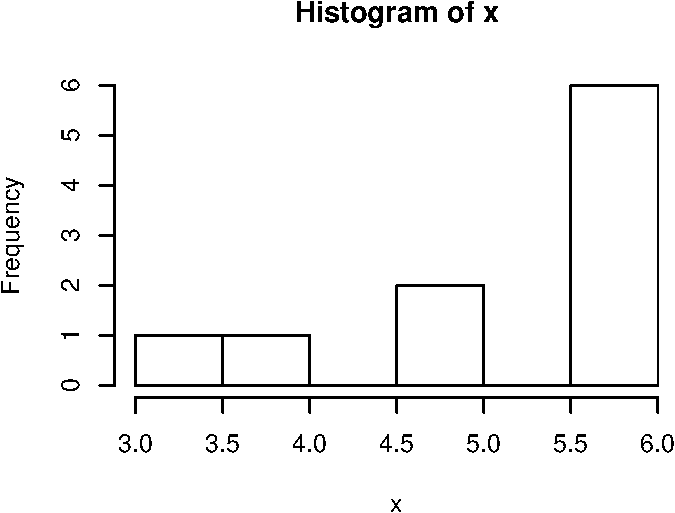
\includegraphics[width=0.5\linewidth]{Rcourse_files/figure-latex/unnamed-chunk-15-1}

R saves every object you create in RAM\footnote{S and S-Plus used to save objects on disk. Working from RAM has advantages and disadvantages. More on this in Chapter \ref{memory}.}.
The collection of all such objects is the \textbf{workspace} which you can inspect with

\begin{Shaded}
\begin{Highlighting}[]
\KeywordTok{ls}\NormalTok{()}
\end{Highlighting}
\end{Shaded}

\begin{verbatim}
## [1] "x"
\end{verbatim}

or with Ctrl+8 in RStudio.

If you lost your object, you can use \texttt{ls} with a text pattern to search for it

\begin{Shaded}
\begin{Highlighting}[]
\KeywordTok{ls}\NormalTok{(}\DataTypeTok{pattern=}\StringTok{'x'}\NormalTok{)}
\end{Highlighting}
\end{Shaded}

\begin{verbatim}
## [1] "x"
\end{verbatim}

To remove objects from the workspace:

\begin{Shaded}
\begin{Highlighting}[]
\KeywordTok{rm}\NormalTok{(x) }\CommentTok{# remove variable}
\KeywordTok{ls}\NormalTok{() }\CommentTok{# verify}
\end{Highlighting}
\end{Shaded}

\begin{verbatim}
## character(0)
\end{verbatim}

You may think that if an object is removed then its memory is freed.
This is almost true, and depends on a negotiation mechanism between R and the operating system.
R's memory management is discussed in Chapter \ref{memory}.

\hypertarget{missing}{%
\section{Missing}\label{missing}}

Unlike typically programming, when working with real life data, you may have \textbf{missing} values: measurements that were simply not recorded/stored/etc.
\emph{R} has rather sophisticated mechanisms to deal with missing values.
It distinguishes between the following types:

\begin{enumerate}
\def\labelenumi{\arabic{enumi}.}
\tightlist
\item
  \texttt{NA}: Not Available entries.
\item
  \texttt{NaN}: Not a number.
\end{enumerate}

\emph{R} tries to defend the analyst, and return an error, or \texttt{NA} when the presence of missing values invalidates the calculation:

\begin{Shaded}
\begin{Highlighting}[]
\NormalTok{missing.example <-}\StringTok{ }\KeywordTok{c}\NormalTok{(}\DecValTok{10}\NormalTok{,}\DecValTok{11}\NormalTok{,}\DecValTok{12}\NormalTok{,}\OtherTok{NA}\NormalTok{)}
\KeywordTok{mean}\NormalTok{(missing.example)}
\end{Highlighting}
\end{Shaded}

\begin{verbatim}
## [1] NA
\end{verbatim}

Most functions will typically have an inner mechanism to deal with these. In the \texttt{mean} function, there is an \texttt{na.rm} argument, telling \emph{R} how to Remove \texttt{NA}s.

\begin{Shaded}
\begin{Highlighting}[]
\KeywordTok{mean}\NormalTok{(missing.example, }\DataTypeTok{na.rm =} \OtherTok{TRUE}\NormalTok{)}
\end{Highlighting}
\end{Shaded}

\begin{verbatim}
## [1] 11
\end{verbatim}

A more general mechanism is removing these manually:

\begin{Shaded}
\begin{Highlighting}[]
\NormalTok{clean.example <-}\StringTok{ }\KeywordTok{na.omit}\NormalTok{(missing.example)}
\KeywordTok{mean}\NormalTok{(clean.example)}
\end{Highlighting}
\end{Shaded}

\begin{verbatim}
## [1] 11
\end{verbatim}

\hypertarget{piping}{%
\section{Piping}\label{piping}}

Because R originates in Unix and Linux environments, it inherits much of its flavor.
\href{http://ryanstutorials.net/linuxtutorial/piping.php}{Piping} is an idea taken from the Linux shell which allows to use the output of one expression as the input to another.
Piping thus makes code easier to read and write.

\BeginKnitrBlock{remark}
\iffalse{} {Remark. } \fi{}Volleyball fans may be confused with the idea of spiking a ball from the 3-meter line, also called \href{https://www.youtube.com/watch?v=DEaj4X_JhSY}{piping}.
So:
(a) These are very different things.
(b) If you can pipe, \href{http://in.bgu.ac.il/sport/Pages/asa.aspx}{ASA-BGU} is looking for you!
\EndKnitrBlock{remark}

Prerequisites:

\begin{Shaded}
\begin{Highlighting}[]
\KeywordTok{library}\NormalTok{(magrittr) }\CommentTok{# load the piping functions}
\NormalTok{x <-}\StringTok{ }\KeywordTok{rbinom}\NormalTok{(}\DataTypeTok{n=}\DecValTok{1000}\NormalTok{, }\DataTypeTok{size=}\DecValTok{10}\NormalTok{, }\DataTypeTok{prob=}\FloatTok{0.5}\NormalTok{) }\CommentTok{# generate some toy data}
\end{Highlighting}
\end{Shaded}

Examples

\begin{Shaded}
\begin{Highlighting}[]
\NormalTok{x }\OperatorTok\StringTok{ }\KeywordTok{var}\NormalTok{() }\CommentTok{# Instead of var(x)}
\NormalTok{x }\OperatorTok\StringTok{ }\KeywordTok{hist}\NormalTok{()  }\CommentTok{# Instead of hist(x)}
\NormalTok{x }\OperatorTok\StringTok{ }\KeywordTok{mean}\NormalTok{() }\OperatorTok\StringTok{ }\KeywordTok{round}\NormalTok{(}\DecValTok{2}\NormalTok{) }\OperatorTok\StringTok{ }\KeywordTok{add}\NormalTok{(}\DecValTok{10}\NormalTok{) }
\end{Highlighting}
\end{Shaded}

The next example\footnote{Taken from \url{http://cran.r-project.org/web/packages/magrittr/vignettes/magrittr.html}} demonstrates the benefits of piping.
The next two chunks of code do the same thing.
Try parsing them in your mind:

\begin{Shaded}
\begin{Highlighting}[]
\CommentTok{# Functional (onion) style}
\NormalTok{car_data <-}\StringTok{ }
\StringTok{  }\KeywordTok{transform}\NormalTok{(}\KeywordTok{aggregate}\NormalTok{(. }\OperatorTok{~}\StringTok{ }\NormalTok{cyl, }
                      \DataTypeTok{data =} \KeywordTok{subset}\NormalTok{(mtcars, hp }\OperatorTok{>}\StringTok{ }\DecValTok{100}\NormalTok{), }
                      \DataTypeTok{FUN =} \ControlFlowTok{function}\NormalTok{(x) }\KeywordTok{round}\NormalTok{(}\KeywordTok{mean}\NormalTok{(x, }\DecValTok{2}\NormalTok{))), }
            \DataTypeTok{kpl =}\NormalTok{ mpg}\OperatorTok{*}\FloatTok{0.4251}\NormalTok{)}
\end{Highlighting}
\end{Shaded}

\begin{Shaded}
\begin{Highlighting}[]
\CommentTok{# Piping (magrittr) style}
\NormalTok{car_data <-}\StringTok{ }
\StringTok{  }\NormalTok{mtcars }\OperatorTok
\StringTok{  }\KeywordTok{subset}\NormalTok{(hp }\OperatorTok{>}\StringTok{ }\DecValTok{100}\NormalTok{) }\OperatorTok
\StringTok{  }\KeywordTok{aggregate}\NormalTok{(. }\OperatorTok{~}\StringTok{ }\NormalTok{cyl, }\DataTypeTok{data =}\NormalTok{ ., }\DataTypeTok{FUN =}\NormalTok{ . }\OperatorTok\StringTok{ }\NormalTok{mean }\OperatorTok\StringTok{ }\KeywordTok{round}\NormalTok{(}\DecValTok{2}\NormalTok{)) }\OperatorTok
\StringTok{  }\KeywordTok{transform}\NormalTok{(}\DataTypeTok{kpl =}\NormalTok{ mpg }\OperatorTok\StringTok{ }\KeywordTok{multiply_by}\NormalTok{(}\FloatTok{0.4251}\NormalTok{)) }\OperatorTok
\StringTok{  }\NormalTok{print}
\end{Highlighting}
\end{Shaded}

Tip: RStudio has a keyboard shortcut for the \texttt{\%\textgreater{}\%} operator. Try Ctrl+Shift+m.

\hypertarget{vector-creation-and-manipulation}{%
\section{Vector Creation and Manipulation}\label{vector-creation-and-manipulation}}

The most basic building block in R is the \textbf{vector}.
We will now see how to create them, and access their elements (i.e.~subsetting).
Here are three ways to create the same arbitrary vector:

\begin{Shaded}
\begin{Highlighting}[]
\KeywordTok{c}\NormalTok{(}\DecValTok{10}\NormalTok{, }\DecValTok{11}\NormalTok{, }\DecValTok{12}\NormalTok{, }\DecValTok{13}\NormalTok{, }\DecValTok{14}\NormalTok{, }\DecValTok{15}\NormalTok{, }\DecValTok{16}\NormalTok{, }\DecValTok{17}\NormalTok{, }\DecValTok{18}\NormalTok{, }\DecValTok{19}\NormalTok{, }\DecValTok{20}\NormalTok{, }\DecValTok{21}\NormalTok{) }\CommentTok{# manually}
\DecValTok{10}\OperatorTok{:}\DecValTok{21} \CommentTok{# the `:` operator                            }
\KeywordTok{seq}\NormalTok{(}\DataTypeTok{from=}\DecValTok{10}\NormalTok{, }\DataTypeTok{to=}\DecValTok{21}\NormalTok{, }\DataTypeTok{by=}\DecValTok{1}\NormalTok{) }\CommentTok{# the seq() function}
\end{Highlighting}
\end{Shaded}

Let's assign it to the object named ``x'':

\begin{Shaded}
\begin{Highlighting}[]
\NormalTok{x <-}\StringTok{ }\KeywordTok{c}\NormalTok{(}\DecValTok{10}\NormalTok{, }\DecValTok{11}\NormalTok{, }\DecValTok{12}\NormalTok{, }\DecValTok{13}\NormalTok{, }\DecValTok{14}\NormalTok{, }\DecValTok{15}\NormalTok{, }\DecValTok{16}\NormalTok{, }\DecValTok{17}\NormalTok{, }\DecValTok{18}\NormalTok{, }\DecValTok{19}\NormalTok{, }\DecValTok{20}\NormalTok{, }\DecValTok{21}\NormalTok{)  }
\end{Highlighting}
\end{Shaded}

Operations usually work element-wise:

\begin{Shaded}
\begin{Highlighting}[]
\NormalTok{x}\OperatorTok{+}\DecValTok{2}
\end{Highlighting}
\end{Shaded}

\begin{verbatim}
##  [1] 12 13 14 15 16 17 18 19 20 21 22 23
\end{verbatim}

\begin{Shaded}
\begin{Highlighting}[]
\NormalTok{x}\OperatorTok{*}\DecValTok{2}    
\end{Highlighting}
\end{Shaded}

\begin{verbatim}
##  [1] 20 22 24 26 28 30 32 34 36 38 40 42
\end{verbatim}

\begin{Shaded}
\begin{Highlighting}[]
\NormalTok{x}\OperatorTok{^}\DecValTok{2}    
\end{Highlighting}
\end{Shaded}

\begin{verbatim}
##  [1] 100 121 144 169 196 225 256 289 324 361 400 441
\end{verbatim}

\begin{Shaded}
\begin{Highlighting}[]
\KeywordTok{sqrt}\NormalTok{(x)  }
\end{Highlighting}
\end{Shaded}

\begin{verbatim}
##  [1] 3.162278 3.316625 3.464102 3.605551 3.741657 3.872983 4.000000
##  [8] 4.123106 4.242641 4.358899 4.472136 4.582576
\end{verbatim}

\begin{Shaded}
\begin{Highlighting}[]
\KeywordTok{log}\NormalTok{(x)   }
\end{Highlighting}
\end{Shaded}

\begin{verbatim}
##  [1] 2.302585 2.397895 2.484907 2.564949 2.639057 2.708050 2.772589
##  [8] 2.833213 2.890372 2.944439 2.995732 3.044522
\end{verbatim}

\hypertarget{search-paths-and-packages}{%
\section{Search Paths and Packages}\label{search-paths-and-packages}}

R can be easily extended with packages, which are merely a set of documented functions, which can be loaded or unloaded conveniently.
Let's look at the function \texttt{read.csv}.
We can see its contents by calling it without arguments:

\begin{Shaded}
\begin{Highlighting}[]
\NormalTok{read.csv}
\end{Highlighting}
\end{Shaded}

\begin{verbatim}
## function (file, header = TRUE, sep = ",", quote = "\"", dec = ".", 
##     fill = TRUE, comment.char = "", ...) 
## read.table(file = file, header = header, sep = sep, quote = quote, 
##     dec = dec, fill = fill, comment.char = comment.char, ...)
## <bytecode: 0x3e49070>
## <environment: namespace:utils>
\end{verbatim}

Never mind what the function does.
Note the \texttt{environment:\ namespace:utils} line at the end.
It tells us that this function is part of the \textbf{utils} package.
We did not need to know this because it is loaded by default.
Here are some packages that I have currently loaded:

\begin{Shaded}
\begin{Highlighting}[]
\KeywordTok{search}\NormalTok{()}
\end{Highlighting}
\end{Shaded}

\begin{verbatim}
##  [1] ".GlobalEnv"           "package:nycflights13" "package:doSNOW"      
##  [4] "package:snow"         "package:doParallel"   "package:parallel"    
##  [7] "package:iterators"    "package:biganalytics" "package:bigmemory"   
## [10] "package:dplyr"        "package:biglm"        "package:DBI"         
## [13] "package:MatrixModels" "package:plotly"       "package:kernlab"     
## [16] "package:scales"       "package:plyr"         "package:class"       
## [19] "package:rpart"        "package:nnet"         "package:e1071"       
## [22] "package:glmnet"       "package:foreach"      "package:ellipse"     
## [25] "package:nlme"         "package:lattice"      "package:lme4"        
## [28] "package:Matrix"       "package:multcomp"     "package:TH.data"     
## [31] "package:survival"     "package:mvtnorm"      "package:MASS"        
## [34] "package:ggalluvial"   "package:ggplot2"      "package:hexbin"      
## [37] "package:data.table"   "package:magrittr"     "tools:rstudio"       
## [40] "package:stats"        "package:graphics"     "package:grDevices"   
## [43] "package:utils"        "package:datasets"     "package:methods"     
## [46] "Autoloads"            "package:base"
\end{verbatim}

Other packages can be loaded via the \texttt{library} function, or downloaded from the internet using the \texttt{install.packages} function before loading with \texttt{library}.
Note that you can easily speedup package download by using multiple CPUs.
Just call \texttt{options(Ncpus\ =\ XXX)}, where \texttt{XXX} is the number of CPUs you want to use.
Run \texttt{parallel::detectCores()} if you are unsure how many CPUs you have on your machine.

\hypertarget{simple-plotting}{%
\section{Simple Plotting}\label{simple-plotting}}

R has many plotting facilities as we will further detail in the Plotting Chapter \ref{plotting}.
We start with the simplest facilities, namely, the \texttt{plot} function from the \textbf{graphics} package, which is loaded by default.

\begin{Shaded}
\begin{Highlighting}[]
\NormalTok{x<-}\StringTok{ }\DecValTok{1}\OperatorTok{:}\DecValTok{100}
\NormalTok{y<-}\StringTok{ }\DecValTok{3}\OperatorTok{+}\KeywordTok{sin}\NormalTok{(x) }
\KeywordTok{plot}\NormalTok{(}\DataTypeTok{x =}\NormalTok{ x, }\DataTypeTok{y =}\NormalTok{ y) }\CommentTok{# x,y syntax                         }
\end{Highlighting}
\end{Shaded}

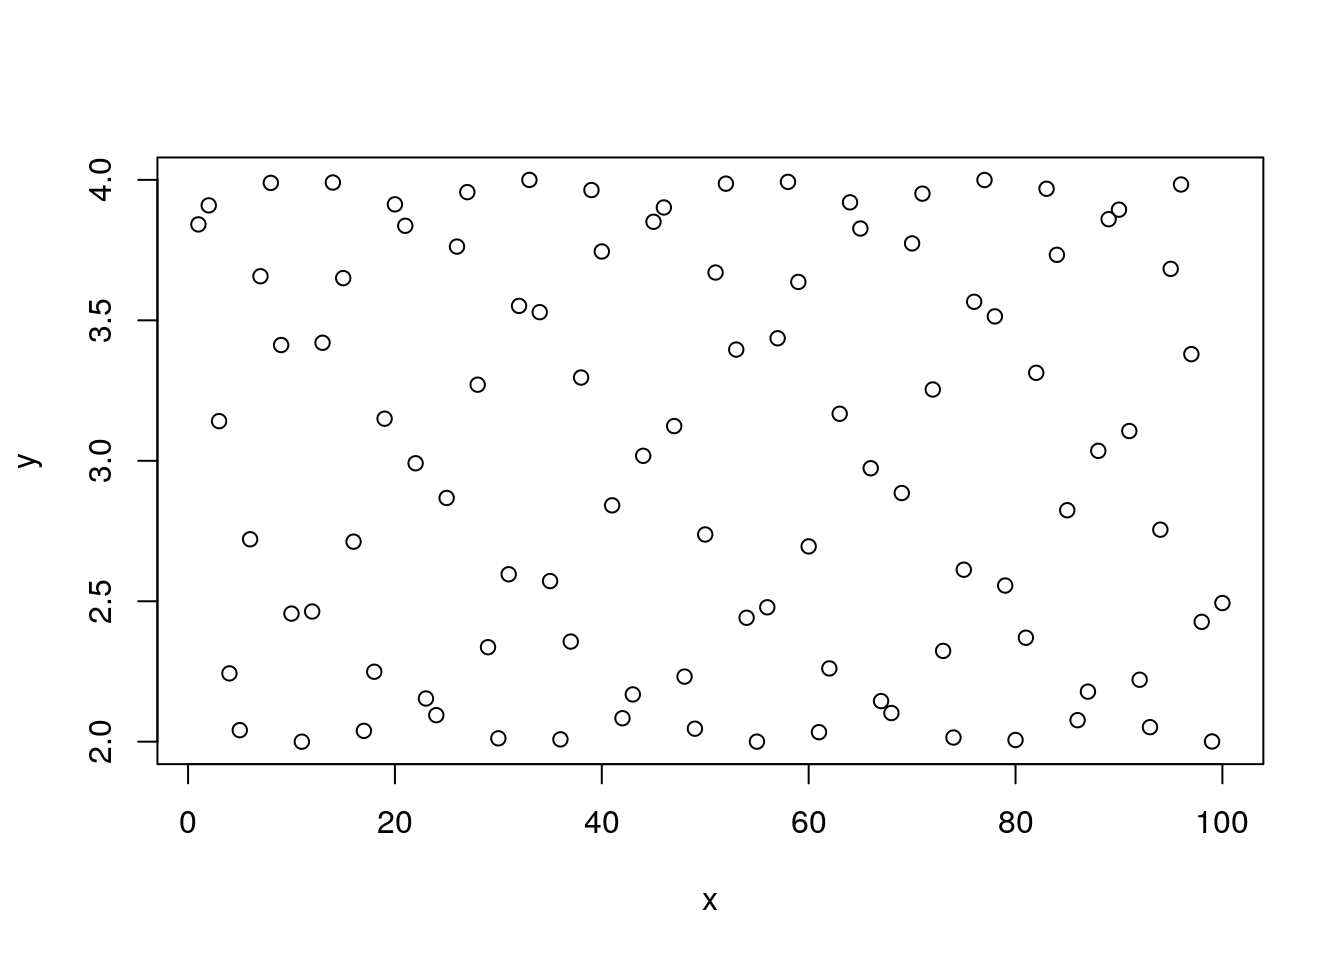
\includegraphics[width=0.5\linewidth]{Rcourse_files/figure-latex/basic-scatter-plot-1}

Given an \texttt{x} argument and a \texttt{y} argument, \texttt{plot} tries to present a scatter plot.
We call this the \texttt{x,y} syntax.
R has another unique syntax to state functional relations.
We call \texttt{y\textasciitilde{}x} the ``tilde'' syntax, which originates in works of \citet{wilkinson1973symbolic} and was adopted in the early days of S.

\begin{Shaded}
\begin{Highlighting}[]
\KeywordTok{plot}\NormalTok{(y }\OperatorTok{~}\StringTok{ }\NormalTok{x, }\DataTypeTok{type=}\StringTok{'l'}\NormalTok{) }\CommentTok{# y~x syntax }
\end{Highlighting}
\end{Shaded}

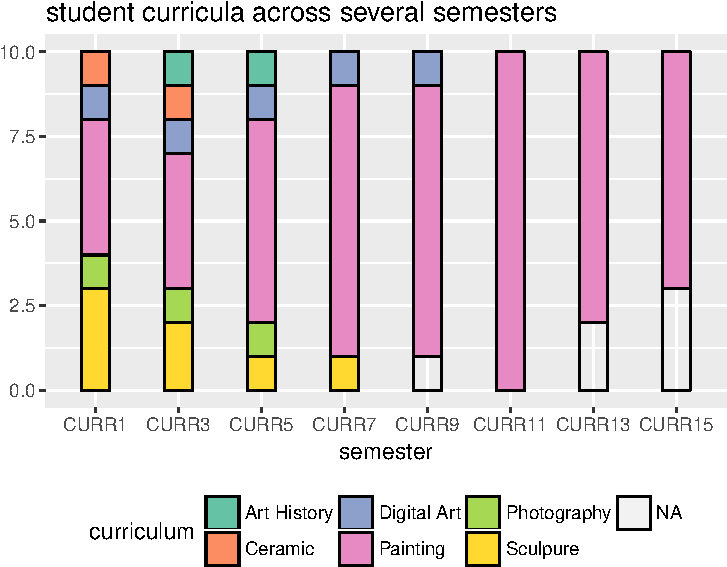
\includegraphics[width=0.5\linewidth]{Rcourse_files/figure-latex/unnamed-chunk-32-1}

The syntax \texttt{y\textasciitilde{}x} is read as ``y is a function of x''.
We will prefer the \texttt{y\textasciitilde{}x} syntax over the \texttt{x,y} syntax since it is easier to read, and will be very useful when we discuss more complicated models.

Here are some arguments that control the plot's appearance.
We use \texttt{type} to control the plot type, \texttt{main} to control the main title.

\begin{Shaded}
\begin{Highlighting}[]
\KeywordTok{plot}\NormalTok{(y}\OperatorTok{~}\NormalTok{x, }\DataTypeTok{type=}\StringTok{'l'}\NormalTok{, }\DataTypeTok{main=}\StringTok{'Plotting a connected line'}\NormalTok{) }
\end{Highlighting}
\end{Shaded}

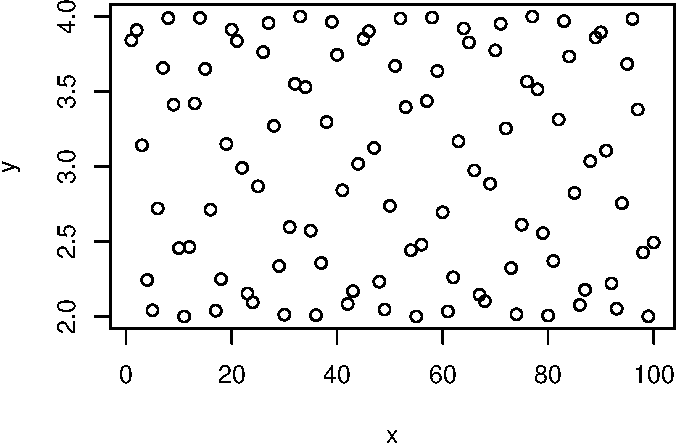
\includegraphics[width=0.5\linewidth]{Rcourse_files/figure-latex/unnamed-chunk-33-1}

We use \texttt{xlab} for the x-axis label, \texttt{ylab} for the y-axis.

\begin{Shaded}
\begin{Highlighting}[]
\KeywordTok{plot}\NormalTok{(y}\OperatorTok{~}\NormalTok{x, }\DataTypeTok{type=}\StringTok{'h'}\NormalTok{, }\DataTypeTok{main=}\StringTok{'Sticks plot'}\NormalTok{, }\DataTypeTok{xlab=}\StringTok{'Insert x axis label'}\NormalTok{, }\DataTypeTok{ylab=}\StringTok{'Insert y axis label'}\NormalTok{) }
\end{Highlighting}
\end{Shaded}

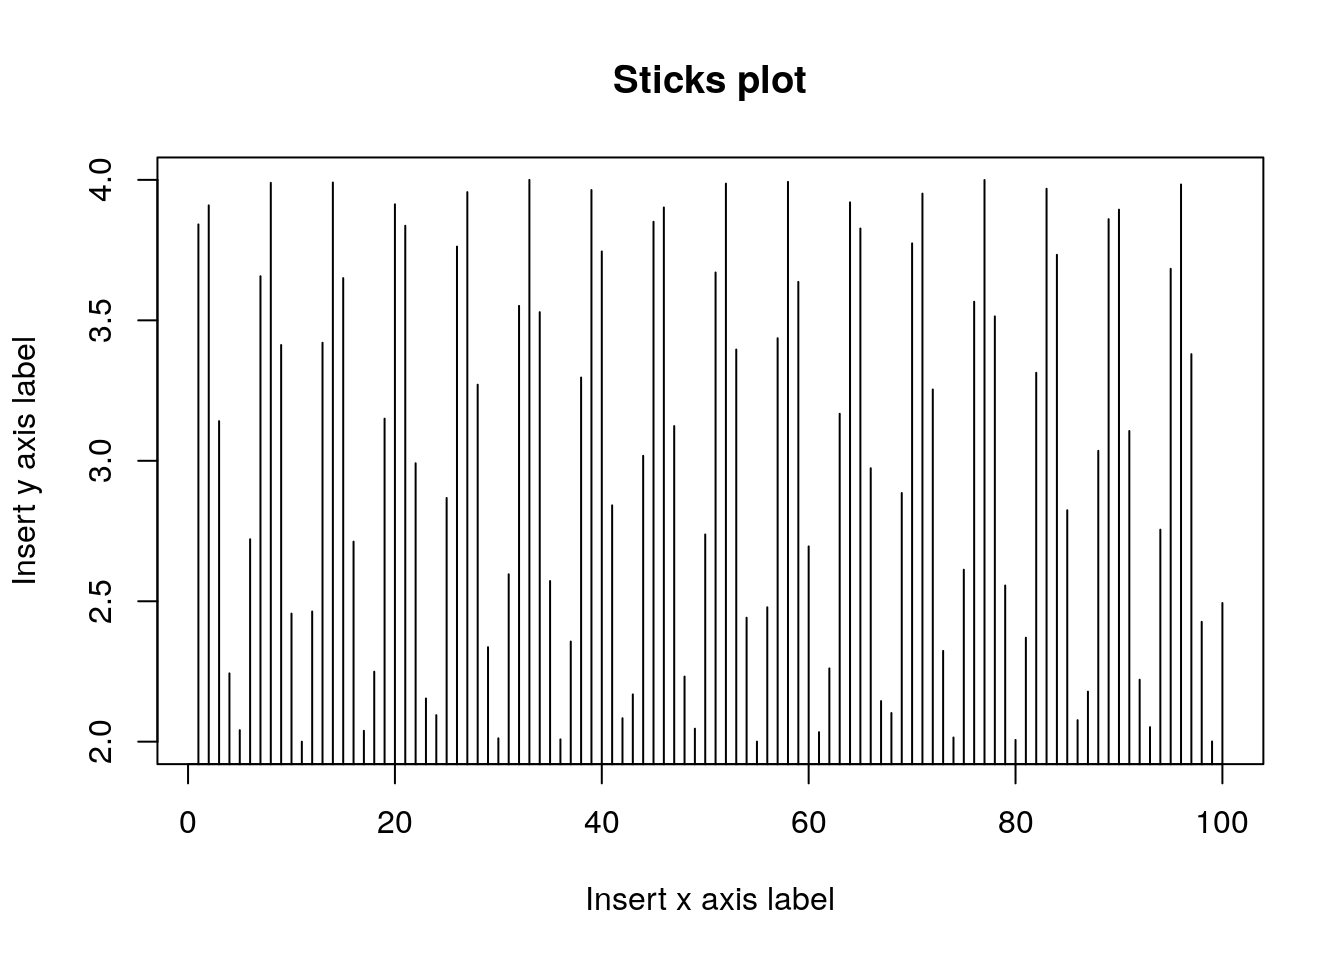
\includegraphics[width=0.5\linewidth]{Rcourse_files/figure-latex/axis-labels-1}

We use \texttt{pch} to control the point type (pch is acronym for Plotting CHaracter).

\begin{Shaded}
\begin{Highlighting}[]
\KeywordTok{plot}\NormalTok{(y}\OperatorTok{~}\NormalTok{x, }\DataTypeTok{pch=}\DecValTok{5}\NormalTok{) }\CommentTok{# Point type with pcf}
\end{Highlighting}
\end{Shaded}

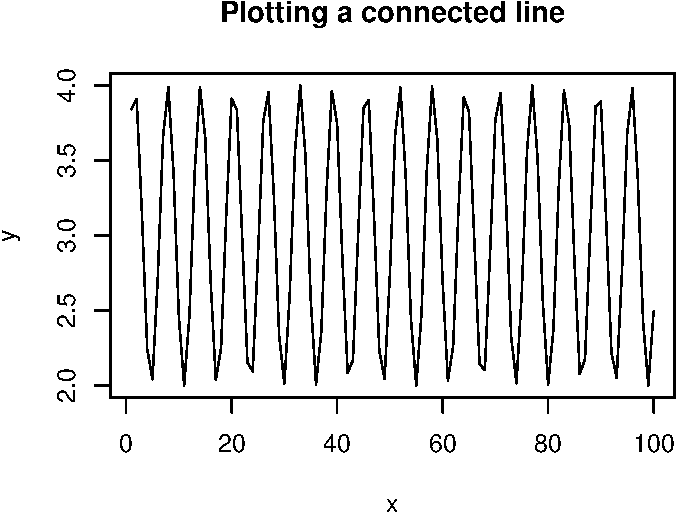
\includegraphics[width=0.5\linewidth]{Rcourse_files/figure-latex/unnamed-chunk-34-1}

We use \texttt{col} to control the color, \texttt{cex} (Character EXpansion) for the point size, and \texttt{abline} (y=Bx+A) to add a straight line.

\begin{Shaded}
\begin{Highlighting}[]
\KeywordTok{plot}\NormalTok{(y}\OperatorTok{~}\NormalTok{x, }\DataTypeTok{pch=}\DecValTok{10}\NormalTok{, }\DataTypeTok{type=}\StringTok{'p'}\NormalTok{, }\DataTypeTok{col=}\StringTok{'blue'}\NormalTok{, }\DataTypeTok{cex=}\DecValTok{4}\NormalTok{) }
\KeywordTok{abline}\NormalTok{(}\DecValTok{3}\NormalTok{, }\FloatTok{0.002}\NormalTok{) }
\end{Highlighting}
\end{Shaded}

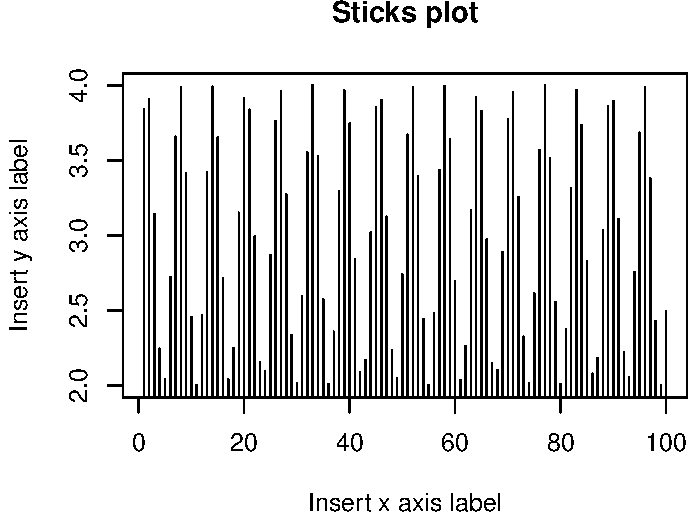
\includegraphics[width=0.5\linewidth]{Rcourse_files/figure-latex/unnamed-chunk-35-1}

For more plotting options run these

\begin{Shaded}
\begin{Highlighting}[]
\KeywordTok{example}\NormalTok{(plot)}
\KeywordTok{example}\NormalTok{(points)}
\NormalTok{?plot}
\KeywordTok{help}\NormalTok{(}\DataTypeTok{package=}\StringTok{'graphics'}\NormalTok{)}
\end{Highlighting}
\end{Shaded}

When your plotting gets serious, go to Chapter \ref{plotting}.

\hypertarget{object-types}{%
\section{Object Types}\label{object-types}}

We already saw that the basic building block of R objects is the vector.
Vectors can be of the following types:

\begin{itemize}
\tightlist
\item
  \textbf{character} Where each element is a string, i.e., a sequence of alphanumeric symbols.
\item
  \textbf{numeric} Where each element is a \href{https://en.wikipedia.org/wiki/Real_number}{real number} in \href{https://en.wikipedia.org/wiki/Double-precision_floating-point_format}{double precision} floating point format.
\item
  \textbf{integer} Where each element is an \href{https://en.wikipedia.org/wiki/Integer}{integer}.
\item
  \textbf{logical} Where each element is either TRUE, FALSE, or NA\footnote{R uses a \href{https://en.wikipedia.org/wiki/Three-valued_logic}{\textbf{three} valued logic} where a missing value (NA) is neither TRUE, nor FALSE.}
\item
  \textbf{complex} Where each element is a complex number.
\item
  \textbf{list} Where each element is an arbitrary R object.
\item
  \textbf{factor} Factors are not actually vector objects, but they feel like such.
  They are used to encode any finite set of values.
  This will be very useful when fitting linear model because they include information on contrasts, i.e., on the encoding of the factors levels.
  You should always be alert and recall when you are dealing with a factor or with a character vector. They have different behaviors.
\end{itemize}

Vectors can be combined into larger objects.
A \texttt{matrix} can be thought of as the binding of several vectors of the same type.
In reality, a matrix is merely a vector with a dimension attribute, that tells R to read it as a matrix and not a vector.

If vectors of different types (but same length) are binded, we get a \texttt{data.frame} which is the most fundamental object in R for data analysis.
Data frames are brilliant, but a lot has been learned since their invention.
They have thus been extended in recent years with the \texttt{tbl} class, pronounced {[}Tibble{]} (\url{https://cran.r-project.org/web/packages/tibble/vignettes/tibble.html}), and the \texttt{data.table} class.\\
The latter is discussed in Chapter \ref{datatable}, and is strongly recommended.

\hypertarget{data-frames}{%
\section{Data Frames}\label{data-frames}}

Creating a simple data frame:

\begin{Shaded}
\begin{Highlighting}[]
\NormalTok{x<-}\StringTok{ }\DecValTok{1}\OperatorTok{:}\DecValTok{10}
\NormalTok{y<-}\StringTok{ }\DecValTok{3} \OperatorTok{+}\StringTok{ }\KeywordTok{sin}\NormalTok{(x) }
\NormalTok{frame1 <-}\StringTok{ }\KeywordTok{data.frame}\NormalTok{(}\DataTypeTok{x=}\NormalTok{x, }\DataTypeTok{sin=}\NormalTok{y)    }
\end{Highlighting}
\end{Shaded}

Let's inspect our data frame:

\begin{Shaded}
\begin{Highlighting}[]
\KeywordTok{head}\NormalTok{(frame1)}
\end{Highlighting}
\end{Shaded}

\begin{verbatim}
##   x      sin
## 1 1 3.841471
## 2 2 3.909297
## 3 3 3.141120
## 4 4 2.243198
## 5 5 2.041076
## 6 6 2.720585
\end{verbatim}

Now using the RStudio Excel-like viewer:

\begin{Shaded}
\begin{Highlighting}[]
\KeywordTok{View}\NormalTok{(frame1) }
\end{Highlighting}
\end{Shaded}

We highly advise against editing the data this way since there will be no documentation of the changes you made.
Always transform your data using scripts, so that everything is documented.

Verifying this is a data frame:

\begin{Shaded}
\begin{Highlighting}[]
\KeywordTok{class}\NormalTok{(frame1) }\CommentTok{# the object is of type data.frame}
\end{Highlighting}
\end{Shaded}

\begin{verbatim}
## [1] "data.frame"
\end{verbatim}

Check the dimension of the data

\begin{Shaded}
\begin{Highlighting}[]
\KeywordTok{dim}\NormalTok{(frame1)                             }
\end{Highlighting}
\end{Shaded}

\begin{verbatim}
## [1] 10  2
\end{verbatim}

Note that checking the dimension of a vector is different than checking the dimension of a data frame.

\begin{Shaded}
\begin{Highlighting}[]
\KeywordTok{length}\NormalTok{(x)}
\end{Highlighting}
\end{Shaded}

\begin{verbatim}
## [1] 10
\end{verbatim}

The length of a \texttt{data.frame} is merely the number of columns.

\begin{Shaded}
\begin{Highlighting}[]
\KeywordTok{length}\NormalTok{(frame1) }
\end{Highlighting}
\end{Shaded}

\begin{verbatim}
## [1] 2
\end{verbatim}

\hypertarget{exctraction}{%
\section{Exctraction}\label{exctraction}}

R provides many ways to subset and extract elements from vectors and other objects.
The basics are fairly simple, but not paying attention to the ``personality'' of each extraction mechanism may cause you a lot of headache.

For starters, extraction is done with the \texttt{{[}} operator.
The operator can take vectors of many types.

Extracting element with by integer index:

\begin{Shaded}
\begin{Highlighting}[]
\NormalTok{frame1[}\DecValTok{1}\NormalTok{, }\DecValTok{2}\NormalTok{]  }\CommentTok{# exctract the element in the 1st row and 2nd column.}
\end{Highlighting}
\end{Shaded}

\begin{verbatim}
## [1] 3.841471
\end{verbatim}

Extract \textbf{column} by index:

\begin{Shaded}
\begin{Highlighting}[]
\NormalTok{frame1[,}\DecValTok{1}\NormalTok{]                              }
\end{Highlighting}
\end{Shaded}

\begin{verbatim}
##  [1]  1  2  3  4  5  6  7  8  9 10
\end{verbatim}

Extract column by name:

\begin{Shaded}
\begin{Highlighting}[]
\NormalTok{frame1[, }\StringTok{'sin'}\NormalTok{]}
\end{Highlighting}
\end{Shaded}

\begin{verbatim}
##  [1] 3.841471 3.909297 3.141120 2.243198 2.041076 2.720585 3.656987
##  [8] 3.989358 3.412118 2.455979
\end{verbatim}

As a general rule, extraction with \texttt{{[}} will conserve the class of the parent object.
There are, however, exceptions.
Notice the extraction mechanism and the class of the output in the following examples.

\begin{Shaded}
\begin{Highlighting}[]
\KeywordTok{class}\NormalTok{(frame1[, }\StringTok{'sin'}\NormalTok{])  }\CommentTok{# extracts a column vector}
\end{Highlighting}
\end{Shaded}

\begin{verbatim}
## [1] "numeric"
\end{verbatim}

\begin{Shaded}
\begin{Highlighting}[]
\KeywordTok{class}\NormalTok{(frame1[}\StringTok{'sin'}\NormalTok{])  }\CommentTok{# extracts a data frame}
\end{Highlighting}
\end{Shaded}

\begin{verbatim}
## [1] "data.frame"
\end{verbatim}

\begin{Shaded}
\begin{Highlighting}[]
\KeywordTok{class}\NormalTok{(frame1[,}\DecValTok{1}\OperatorTok{:}\DecValTok{2}\NormalTok{])  }\CommentTok{# extracts a data frame}
\end{Highlighting}
\end{Shaded}

\begin{verbatim}
## [1] "data.frame"
\end{verbatim}

\begin{Shaded}
\begin{Highlighting}[]
\KeywordTok{class}\NormalTok{(frame1[}\DecValTok{2}\NormalTok{])  }\CommentTok{# extracts a data frame}
\end{Highlighting}
\end{Shaded}

\begin{verbatim}
## [1] "data.frame"
\end{verbatim}

\begin{Shaded}
\begin{Highlighting}[]
\KeywordTok{class}\NormalTok{(frame1[}\DecValTok{2}\NormalTok{, ])  }\CommentTok{# extract a data frame}
\end{Highlighting}
\end{Shaded}

\begin{verbatim}
## [1] "data.frame"
\end{verbatim}

\begin{Shaded}
\begin{Highlighting}[]
\KeywordTok{class}\NormalTok{(frame1}\OperatorTok{$}\NormalTok{sin)  }\CommentTok{# extracts a column vector}
\end{Highlighting}
\end{Shaded}

\begin{verbatim}
## [1] "numeric"
\end{verbatim}

The \texttt{subset()} function does the same

\begin{Shaded}
\begin{Highlighting}[]
\KeywordTok{subset}\NormalTok{(frame1, }\DataTypeTok{select=}\NormalTok{sin) }
\KeywordTok{subset}\NormalTok{(frame1, }\DataTypeTok{select=}\DecValTok{2}\NormalTok{)}
\KeywordTok{subset}\NormalTok{(frame1, }\DataTypeTok{select=} \KeywordTok{c}\NormalTok{(}\DecValTok{2}\NormalTok{,}\DecValTok{0}\NormalTok{))}
\end{Highlighting}
\end{Shaded}

If you want to force the stripping of the class attribute when extracting, try the \texttt{{[}{[}} mechanism instead of \texttt{{[}}.

\begin{Shaded}
\begin{Highlighting}[]
\NormalTok{a <-}\StringTok{ }\NormalTok{frame1[}\DecValTok{1}\NormalTok{] }\CommentTok{# [ extraction}
\NormalTok{b <-}\StringTok{ }\NormalTok{frame1[[}\DecValTok{1}\NormalTok{]] }\CommentTok{# [[ extraction}
\KeywordTok{class}\NormalTok{(a)}\OperatorTok{==}\KeywordTok{class}\NormalTok{(b) }\CommentTok{# objects have differing classes}
\end{Highlighting}
\end{Shaded}

\begin{verbatim}
## [1] FALSE
\end{verbatim}

\begin{Shaded}
\begin{Highlighting}[]
\NormalTok{a}\OperatorTok{==}\NormalTok{b }\CommentTok{# objects are element-wise identical }
\end{Highlighting}
\end{Shaded}

\begin{verbatim}
##          x
##  [1,] TRUE
##  [2,] TRUE
##  [3,] TRUE
##  [4,] TRUE
##  [5,] TRUE
##  [6,] TRUE
##  [7,] TRUE
##  [8,] TRUE
##  [9,] TRUE
## [10,] TRUE
\end{verbatim}

The different types of output classes cause different behaviors. Compare the behavior of \texttt{{[}} on seemingly identical objects.

\begin{Shaded}
\begin{Highlighting}[]
\NormalTok{frame1[}\DecValTok{1}\NormalTok{][}\DecValTok{1}\NormalTok{]}
\end{Highlighting}
\end{Shaded}

\begin{verbatim}
##     x
## 1   1
## 2   2
## 3   3
## 4   4
## 5   5
## 6   6
## 7   7
## 8   8
## 9   9
## 10 10
\end{verbatim}

\begin{Shaded}
\begin{Highlighting}[]
\NormalTok{frame1[[}\DecValTok{1}\NormalTok{]][}\DecValTok{1}\NormalTok{]}
\end{Highlighting}
\end{Shaded}

\begin{verbatim}
## [1] 1
\end{verbatim}

If you want to learn more about subsetting see \href{http://adv-r.had.co.nz/Subsetting.html}{Hadley's guide}.

\hypertarget{augmentations-of-the-data.frame-class}{%
\section{Augmentations of the data.frame class}\label{augmentations-of-the-data.frame-class}}

As previously mentioned, the \texttt{data.frame} class has been extended in recent years.
The best known extensions are the \texttt{data.table} and the \texttt{tbl}.
For beginners, it is important to know R's basics, so we keep focusing on data frames.
For more advanced users, I recommend learning the (amazing) \texttt{data.table} syntax.

\hypertarget{data-import-and-export}{%
\section{Data Import and Export}\label{data-import-and-export}}

For any practical purpose, you will not be generating your data manually.
R comes with many importing and exporting mechanisms which we now present.
If, however, you do a lot of data ``munging'', make sure to see Hadley-verse Chapter \ref{hadley}.
If you work with MASSIVE data sets, read the Memory Efficiency Chapter \ref{memory}.

\hypertarget{import-from-web}{%
\subsection{Import from WEB}\label{import-from-web}}

The \texttt{read.table} function is the main importing workhorse.
It can import directly from the web.

\begin{Shaded}
\begin{Highlighting}[]
\NormalTok{URL <-}\StringTok{ 'http://statweb.stanford.edu/~tibs/ElemStatLearn/datasets/bone.data'}
\NormalTok{tirgul1 <-}\StringTok{ }\KeywordTok{read.table}\NormalTok{(URL)}
\end{Highlighting}
\end{Shaded}

Always look at the imported result!

\begin{Shaded}
\begin{Highlighting}[]
\KeywordTok{head}\NormalTok{(tirgul1)}
\end{Highlighting}
\end{Shaded}

\begin{verbatim}
##      V1    V2     V3          V4
## 1 idnum   age gender      spnbmd
## 2     1  11.7   male  0.01808067
## 3     1  12.7   male  0.06010929
## 4     1 13.75   male 0.005857545
## 5     2 13.25   male  0.01026393
## 6     2  14.3   male   0.2105263
\end{verbatim}

Oh dear.
\texttt{read.,table} tried to guess the structure of the input, but failed to recognize the header row. Set it manually with \texttt{header=TRUE}:

\begin{Shaded}
\begin{Highlighting}[]
\NormalTok{tirgul1 <-}\StringTok{ }\KeywordTok{read.table}\NormalTok{(}\StringTok{'data/bone.data'}\NormalTok{, }\DataTypeTok{header =} \OtherTok{TRUE}\NormalTok{) }
\KeywordTok{head}\NormalTok{(tirgul1)}
\end{Highlighting}
\end{Shaded}

\hypertarget{import-from-clipboard}{%
\subsection{Import From Clipboard}\label{import-from-clipboard}}

TODO:\href{https://github.com/MilesMcBain/datapasta}{datapasta}

\hypertarget{export-as-csv}{%
\subsection{Export as CSV}\label{export-as-csv}}

Let's write a simple file so that we have something to import

\begin{Shaded}
\begin{Highlighting}[]
\KeywordTok{head}\NormalTok{(airquality) }\CommentTok{#  examine the data to export}
\end{Highlighting}
\end{Shaded}

\begin{verbatim}
##   Ozone Solar.R Wind Temp Month Day
## 1    41     190  7.4   67     5   1
## 2    36     118  8.0   72     5   2
## 3    12     149 12.6   74     5   3
## 4    18     313 11.5   62     5   4
## 5    NA      NA 14.3   56     5   5
## 6    28      NA 14.9   66     5   6
\end{verbatim}

\begin{Shaded}
\begin{Highlighting}[]
\NormalTok{temp.file.name <-}\StringTok{ }\KeywordTok{tempfile}\NormalTok{() }\CommentTok{# get some arbitrary file name}
\KeywordTok{write.csv}\NormalTok{(}\DataTypeTok{x =}\NormalTok{ airquality, }\DataTypeTok{file =}\NormalTok{ temp.file.name) }\CommentTok{# export}
\end{Highlighting}
\end{Shaded}

Now let's import the exported file. Being a .csv file, I can use \texttt{read.csv} instead of \texttt{read.table}.

\begin{Shaded}
\begin{Highlighting}[]
\NormalTok{my.data<-}\StringTok{ }\KeywordTok{read.csv}\NormalTok{(}\DataTypeTok{file=}\NormalTok{temp.file.name) }\CommentTok{# import}
\KeywordTok{head}\NormalTok{(my.data) }\CommentTok{# verify import}
\end{Highlighting}
\end{Shaded}

\begin{verbatim}
##   X Ozone Solar.R Wind Temp Month Day
## 1 1    41     190  7.4   67     5   1
## 2 2    36     118  8.0   72     5   2
## 3 3    12     149 12.6   74     5   3
## 4 4    18     313 11.5   62     5   4
## 5 5    NA      NA 14.3   56     5   5
## 6 6    28      NA 14.9   66     5   6
\end{verbatim}

\BeginKnitrBlock{remark}
\iffalse{} {Remark. } \fi{}Windows users may need to use ``\textbackslash{}'' instead of ``/''.
\EndKnitrBlock{remark}

\hypertarget{export-non-csv-files}{%
\subsection{Export non-CSV files}\label{export-non-csv-files}}

You can export your R objects in endlessly many ways:
If instead of the comma delimiter in .csv you want other column delimiters, look into \texttt{?write.table}.
If you are exporting only for R users, you can consider exporting as binary objects with \texttt{saveRDS}, \texttt{feather::write\_feather}, or \texttt{fst::write.fst}.
See (\url{http://www.fstpackage.org/}) for a comparison.

\hypertarget{reading-from-text-files}{%
\subsection{Reading From Text Files}\label{reading-from-text-files}}

Some general notes on importing text files via the \texttt{read.table} function.
But first, we need to know what is the active directory.
Here is how to get and set R's active directory:

\begin{Shaded}
\begin{Highlighting}[]
\KeywordTok{getwd}\NormalTok{() }\CommentTok{#What is the working directory?}
\KeywordTok{setwd}\NormalTok{() }\CommentTok{#Setting the working directory in Linux}
\end{Highlighting}
\end{Shaded}

We can now call the \texttt{read.table} function to import text files.
If you care about your sanity, see \texttt{?read.table} before starting imports.
Some notable properties of the function:

\begin{itemize}
\tightlist
\item
  \texttt{read.table} will try to guess column separators (tab, comma, etc.)
\item
  \texttt{read.table} will try to guess if a header row is present.
\item
  \texttt{read.table} will convert character vectors to factors unless told not to using the \texttt{stringsAsFactors=FALSE} argument.
\item
  The output of \texttt{read.table} needs to be explicitly assigned to an object for it to be saved.
\end{itemize}

\hypertarget{writing-data-to-text-files}{%
\subsection{Writing Data to Text Files}\label{writing-data-to-text-files}}

The function \texttt{write.table} is the exporting counterpart of \texttt{read.table}.

\hypertarget{xlsx-files}{%
\subsection{.XLS(X) files}\label{xlsx-files}}

Strongly recommended to convert to .csv in Excel, and then import as csv.
If you still insist see the \textbf{xlsx} package.

\hypertarget{massive-files}{%
\subsection{Massive files}\label{massive-files}}

The above importing and exporting mechanisms were not designed for massive files.
An import function that were designed for large files is \href{https://github.com/r-lib/vroom}{vroom}.
But also see the sections on the \textbf{data.table} package (\ref{datatable}), Sparse Representation (\ref{sparse}), and Out-of-Ram Algorithms (\ref{memory}) for more on working with massive data files.

\hypertarget{databases}{%
\subsection{Databases}\label{databases}}

R does not need to read from text files; it can read directly from a database.
This is very useful since it allows the filtering, selecting and joining operations to rely on the database's optimized algorithms.
Then again, if you will only be analyzing your data with R, you are probably better of by working from a file, without the databases' overhead.
See Chapter \ref{memory} for more on this matter.

\hypertarget{functions}{%
\section{Functions}\label{functions}}

One of the most basic building blocks of programming is the ability of writing your own functions.
A function in R, like everything else, is an object accessible using its name.
We first define a simple function that sums its two arguments

\begin{Shaded}
\begin{Highlighting}[]
\NormalTok{my.sum <-}\StringTok{ }\ControlFlowTok{function}\NormalTok{(x,y) \{}
  \KeywordTok{return}\NormalTok{(x}\OperatorTok{+}\NormalTok{y)}
\NormalTok{\}}
\KeywordTok{my.sum}\NormalTok{(}\DecValTok{10}\NormalTok{,}\DecValTok{2}\NormalTok{)}
\end{Highlighting}
\end{Shaded}

\begin{verbatim}
## [1] 12
\end{verbatim}

From this example you may notice that:

\begin{itemize}
\item
  The function \texttt{function} tells R to construct a function object.
\item
  Unlike some programming languages, a period (\texttt{.}) is allowed as part of an object's name.
\item
  The arguments of the \texttt{function}, i.e. \texttt{(x,y)}, need to be named but we are not required to specify their class. This makes writing functions very easy, but it is also the source of many bugs, and slowness of R compared to type declaring languages (C, Fortran,Java,\ldots{}).
\item
  A typical R function does not change objects\footnote{This is a classical \emph{functional programming} paradigm. If you want an object oriented flavor of R programming, see Hadley's \href{http://adv-r.had.co.nz/OO-essentials.html}{Advanced R book}.} but rather creates new ones.
  To save the output of \texttt{my.sum} we will need to assign it using the \texttt{\textless{}-} operator.
\end{itemize}

Here is a (slightly) more advanced function:

\begin{Shaded}
\begin{Highlighting}[]
\NormalTok{my.sum}\FloatTok{.2}\NormalTok{ <-}\StringTok{ }\ControlFlowTok{function}\NormalTok{(x, y , }\DataTypeTok{absolute=}\OtherTok{FALSE}\NormalTok{) \{}
  \ControlFlowTok{if}\NormalTok{(absolute}\OperatorTok{==}\OtherTok{TRUE}\NormalTok{) \{}
\NormalTok{    result <-}\StringTok{ }\KeywordTok{abs}\NormalTok{(x}\OperatorTok{+}\NormalTok{y)}
\NormalTok{  \}}
  \ControlFlowTok{else}\NormalTok{\{}
\NormalTok{    result <-}\StringTok{ }\NormalTok{x}\OperatorTok{+}\NormalTok{y}
\NormalTok{  \} }
\NormalTok{  result}
\NormalTok{\}}
\KeywordTok{my.sum.2}\NormalTok{(}\OperatorTok{-}\DecValTok{10}\NormalTok{,}\DecValTok{2}\NormalTok{,}\OtherTok{TRUE}\NormalTok{)}
\end{Highlighting}
\end{Shaded}

\begin{verbatim}
## [1] 8
\end{verbatim}

Things to note:

\begin{itemize}
\item
  \texttt{if(condition)\{expression1\}\ else\{expression2\}} does just what the name suggests.
\item
  The function will output its last evaluated expression. You don't need to use the \texttt{return} function explicitly.
\item
  Using \texttt{absolute=FALSE} sets the default value of \texttt{absolute} to \texttt{FALSE}. This is overridden if \texttt{absolute} is stated explicitly in the function call.
\end{itemize}

An important behavior of R is the \emph{scoping rules}.
This refers to the way R seeks for variables used in functions.
As a rule of thumb, R will first look for variables inside the function and if not found, will search for the variable values in outer environments\footnote{More formally, this is called \href{https://darrenjw.wordpress.com/2011/11/23/lexical-scope-and-function-closures-in-r/}{Lexical Scoping}.}.
Think of the next example.

\begin{Shaded}
\begin{Highlighting}[]
\NormalTok{a <-}\StringTok{ }\DecValTok{1}
\NormalTok{b <-}\StringTok{ }\DecValTok{2}
\NormalTok{x <-}\StringTok{ }\DecValTok{3}
\NormalTok{scoping <-}\StringTok{ }\ControlFlowTok{function}\NormalTok{(a,b)\{}
\NormalTok{  a}\OperatorTok{+}\NormalTok{b}\OperatorTok{+}\NormalTok{x}
\NormalTok{\}}
\KeywordTok{scoping}\NormalTok{(}\DecValTok{10}\NormalTok{,}\DecValTok{11}\NormalTok{)}
\end{Highlighting}
\end{Shaded}

\begin{verbatim}
## [1] 24
\end{verbatim}

\hypertarget{looping}{%
\section{Looping}\label{looping}}

The real power of scripting is when repeated operations are done by iteration.
R supports the usual \texttt{for}, \texttt{while}, and \texttt{repated} loops.
Here is an embarrassingly simple example

\begin{Shaded}
\begin{Highlighting}[]
\ControlFlowTok{for}\NormalTok{ (i }\ControlFlowTok{in} \DecValTok{1}\OperatorTok{:}\DecValTok{5}\NormalTok{)\{}
    \KeywordTok{print}\NormalTok{(i)}
\NormalTok{    \}}
\end{Highlighting}
\end{Shaded}

\begin{verbatim}
## [1] 1
## [1] 2
## [1] 3
## [1] 4
## [1] 5
\end{verbatim}

A slightly more advanced example, is vector multiplication

\begin{Shaded}
\begin{Highlighting}[]
\NormalTok{result <-}\StringTok{ }\DecValTok{0}
\NormalTok{n <-}\StringTok{ }\FloatTok{1e3}
\NormalTok{x <-}\StringTok{ }\DecValTok{1}\OperatorTok{:}\NormalTok{n}
\NormalTok{y <-}\StringTok{ }\NormalTok{(}\DecValTok{1}\OperatorTok{:}\NormalTok{n)}\OperatorTok{/}\NormalTok{n}
\ControlFlowTok{for}\NormalTok{(i }\ControlFlowTok{in} \DecValTok{1}\OperatorTok{:}\NormalTok{n)\{}
\NormalTok{  result <-}\StringTok{ }\NormalTok{result}\OperatorTok{+}\StringTok{ }\NormalTok{x[i]}\OperatorTok{*}\NormalTok{y[i]}
\NormalTok{\}}
\end{Highlighting}
\end{Shaded}

\BeginKnitrBlock{remark}
\iffalse{} {Remark. } \fi{}\textbf{Vector Operations}:
You should NEVER write your own vector and matrix products like in the previous example. Only use existing facilities such as \texttt{\%*\%}, \texttt{sum()}, etc.
\EndKnitrBlock{remark}

\BeginKnitrBlock{remark}
\iffalse{} {Remark. } \fi{}\textbf{Parallel Operations}:
If you already know that you will be needing to parallelize your work, get used to working with \texttt{foreach} loops in the \textbf{foreach} package, rather then regular \texttt{for} loops.
\EndKnitrBlock{remark}

\hypertarget{apply}{%
\section{Apply}\label{apply}}

For applying the same function to a set of elements, there is no need to write an explicit loop.
This is such an elementary operation that every programming language will provide some facility to \textbf{apply}, or \textbf{map} the function to all elements of a set.
R provides several facilities to perform this.
The most basic of which is \texttt{lapply} which applies a function over all elements of a list, and return a list of outputs:

\begin{Shaded}
\begin{Highlighting}[]
\NormalTok{the.list <-}\StringTok{ }\KeywordTok{list}\NormalTok{(}\DecValTok{1}\NormalTok{,}\StringTok{'a'}\NormalTok{,mean) }\CommentTok{# a list of 3 elements from different classes}
\KeywordTok{lapply}\NormalTok{(}\DataTypeTok{X =}\NormalTok{ the.list, }\DataTypeTok{FUN =}\NormalTok{ class) }\CommentTok{# apply the function `class` to each elements}
\end{Highlighting}
\end{Shaded}

\begin{verbatim}
## [[1]]
## [1] "numeric"
## 
## [[2]]
## [1] "character"
## 
## [[3]]
## [1] "standardGeneric"
## attr(,"package")
## [1] "methods"
\end{verbatim}

\begin{Shaded}
\begin{Highlighting}[]
\KeywordTok{sapply}\NormalTok{(}\DataTypeTok{X =}\NormalTok{ the.list, }\DataTypeTok{FUN =}\NormalTok{ class) }\CommentTok{# lapply with cleaned output}
\end{Highlighting}
\end{Shaded}

\begin{verbatim}
## [1] "numeric"         "character"       "standardGeneric"
\end{verbatim}

What is the function you are using requires some arguments?
One useful trick is to create your own function that takes only one argument:

\begin{Shaded}
\begin{Highlighting}[]
\NormalTok{quantile}\FloatTok{.25}\NormalTok{ <-}\StringTok{ }\ControlFlowTok{function}\NormalTok{(x) }\KeywordTok{quantile}\NormalTok{(x,}\FloatTok{0.25}\NormalTok{)}
\KeywordTok{sapply}\NormalTok{(USArrests, quantile}\FloatTok{.25}\NormalTok{)}
\end{Highlighting}
\end{Shaded}

\begin{verbatim}
##   Murder.25%  Assault.25% UrbanPop.25%     Rape.25% 
##        4.075      109.000       54.500       15.075
\end{verbatim}

What if you are applying the same function with \textbf{two} lists of arguments? Use \textbf{mapply}.
The following will compute a different quantile to each column in the data:

\begin{Shaded}
\begin{Highlighting}[]
\NormalTok{quantiles <-}\StringTok{ }\KeywordTok{c}\NormalTok{(}\FloatTok{0.1}\NormalTok{, }\FloatTok{0.5}\NormalTok{, }\FloatTok{0.3}\NormalTok{, }\FloatTok{0.2}\NormalTok{)}
\KeywordTok{mapply}\NormalTok{(quantile, USArrests, quantiles)}
\end{Highlighting}
\end{Shaded}

\begin{verbatim}
##   Murder.10%  Assault.50% UrbanPop.30%     Rape.20% 
##         2.56       159.00        57.70        13.92
\end{verbatim}

R provides many variations on \texttt{lapply} to facilitate programming.
Here is a partial list:

\begin{itemize}
\tightlist
\item
  \texttt{sapply}: The same as \texttt{lapply} but tries to arrange output in a vector or matrix, and not an unstructured list.
\item
  \texttt{vapply}: A safer version of \texttt{sapply}, where the output class is pre-specified.
\item
  \texttt{apply}: For applying over the rows or columns of matrices.
\item
  \texttt{mapply}: For applying functions with more than a single input.
\item
  \texttt{tapply}: For splitting vectors and applying functions on subsets.
\item
  \texttt{rapply}: A recursive version of \texttt{lapply}.
\item
  \texttt{eapply}: Like \texttt{lapply}, only operates on \texttt{environments} instead of lists.
\item
  \texttt{Map}+\texttt{Reduce}: For a \href{https://en.wikipedia.org/wiki/Common_Lisp}{Common Lisp} look and feel of \texttt{lapply}.
\item
  \texttt{parallel::parLapply}: A parallel version of \texttt{lapply} from the package \textbf{parallel}.
\item
  \texttt{parallel::parLBapply}: A parallel version of \texttt{lapply}, with load balancing from the package \textbf{parallel}.
\end{itemize}

\hypertarget{recursion}{%
\section{Recursion}\label{recursion}}

The R compiler is really not designed for recursion, and you will rarely need to do so.\\
See the RCpp Chapter \ref{rcpp} for linking C code, which is better suited for recursion.
If you really insist to write recursions in R, make sure to use the \texttt{Recall} function, which, as the name suggests, recalls the function in which it is place.
Here is a demonstration with the Fibonacci series.

\begin{Shaded}
\begin{Highlighting}[]
\NormalTok{fib<-}\ControlFlowTok{function}\NormalTok{(n) \{}
    \ControlFlowTok{if}\NormalTok{ (n }\OperatorTok{<=}\StringTok{ }\DecValTok{2}\NormalTok{) fn<-}\DecValTok{1} 
    \ControlFlowTok{else}\NormalTok{ fn <-}\StringTok{ }\KeywordTok{Recall}\NormalTok{(n }\OperatorTok{-}\StringTok{ }\DecValTok{1}\NormalTok{) }\OperatorTok{+}\StringTok{ }\KeywordTok{Recall}\NormalTok{(n }\OperatorTok{-}\StringTok{ }\DecValTok{2}\NormalTok{) }
    \KeywordTok{return}\NormalTok{(fn)}
\NormalTok{\} }
\KeywordTok{fib}\NormalTok{(}\DecValTok{5}\NormalTok{)}
\end{Highlighting}
\end{Shaded}

\begin{verbatim}
## [1] 5
\end{verbatim}

\hypertarget{strings}{%
\section{Strings}\label{strings}}

Note: this section is courtesy of Ron Sarafian.

Strings may appear as character vectors,files names, paths (directories), graphing elements, and more.

Strings can be concatenated with the super useful \texttt{paste} function.

\begin{Shaded}
\begin{Highlighting}[]
\NormalTok{a <-}\StringTok{ "good"}
\NormalTok{b <-}\StringTok{ "morning"}
\KeywordTok{is.character}\NormalTok{(a)}
\end{Highlighting}
\end{Shaded}

\begin{verbatim}
## [1] TRUE
\end{verbatim}

\begin{Shaded}
\begin{Highlighting}[]
\KeywordTok{paste}\NormalTok{(a,b)}
\end{Highlighting}
\end{Shaded}

\begin{verbatim}
## [1] "good morning"
\end{verbatim}

\begin{Shaded}
\begin{Highlighting}[]
\NormalTok{(c <-}\StringTok{ }\KeywordTok{paste}\NormalTok{(a,b, }\DataTypeTok{sep =} \StringTok{"."}\NormalTok{))}
\end{Highlighting}
\end{Shaded}

\begin{verbatim}
## [1] "good.morning"
\end{verbatim}

\begin{Shaded}
\begin{Highlighting}[]
\KeywordTok{paste}\NormalTok{(a,b,}\DecValTok{1}\OperatorTok{:}\DecValTok{3}\NormalTok{, }\DataTypeTok{paste=}\StringTok{'@@@'}\NormalTok{, }\DataTypeTok{collapse =} \StringTok{'^^^^'}\NormalTok{)}
\end{Highlighting}
\end{Shaded}

\begin{verbatim}
## [1] "good morning 1 @@@^^^^good morning 2 @@@^^^^good morning 3 @@@"
\end{verbatim}

Things to note:

\begin{itemize}
\tightlist
\item
  \texttt{sep} is used to separate strings.
\item
  \texttt{collapse} is used to separate results.
\end{itemize}

The \texttt{substr} function extract or replace substrings in a character vector:

\begin{Shaded}
\begin{Highlighting}[]
\KeywordTok{substr}\NormalTok{(c, }\DataTypeTok{start=}\DecValTok{2}\NormalTok{, }\DataTypeTok{stop=}\DecValTok{4}\NormalTok{)}
\end{Highlighting}
\end{Shaded}

\begin{verbatim}
## [1] "ood"
\end{verbatim}

\begin{Shaded}
\begin{Highlighting}[]
\KeywordTok{substr}\NormalTok{(c, }\DataTypeTok{start=}\DecValTok{6}\NormalTok{, }\DataTypeTok{stop=}\DecValTok{12}\NormalTok{) <-}\StringTok{ "evening"}
\end{Highlighting}
\end{Shaded}

The \texttt{grep} function is a very powerful tool to search for patterns in text.
These patterns are called \href{https://en.wikipedia.org/wiki/Regular_expression}{regular expressions}

\begin{Shaded}
\begin{Highlighting}[]
\NormalTok{(d <-}\StringTok{ }\KeywordTok{c}\NormalTok{(a,b,c))}
\end{Highlighting}
\end{Shaded}

\begin{verbatim}
## [1] "good"         "morning"      "good.evening"
\end{verbatim}

\begin{Shaded}
\begin{Highlighting}[]
\KeywordTok{grep}\NormalTok{(}\DataTypeTok{pattern =} \StringTok{"good"}\NormalTok{,}\DataTypeTok{x =}\NormalTok{ d) }
\end{Highlighting}
\end{Shaded}

\begin{verbatim}
## [1] 1 3
\end{verbatim}

\begin{Shaded}
\begin{Highlighting}[]
\KeywordTok{grep}\NormalTok{(}\StringTok{"good"}\NormalTok{,d, }\DataTypeTok{value=}\OtherTok{TRUE}\NormalTok{, }\DataTypeTok{ignore.case=}\OtherTok{TRUE}\NormalTok{) }
\end{Highlighting}
\end{Shaded}

\begin{verbatim}
## [1] "good"         "good.evening"
\end{verbatim}

\begin{Shaded}
\begin{Highlighting}[]
\KeywordTok{grep}\NormalTok{(}\StringTok{"([a-zA-Z]+)}\CharTok{\textbackslash{}\textbackslash{}}\StringTok{1"}\NormalTok{,d, }\DataTypeTok{value=}\OtherTok{TRUE}\NormalTok{, }\DataTypeTok{perl=}\OtherTok{TRUE}\NormalTok{) }
\end{Highlighting}
\end{Shaded}

\begin{verbatim}
## [1] "good"         "good.evening"
\end{verbatim}

Things to note:

\begin{itemize}
\tightlist
\item
  Use \texttt{value=TRUE} to return the string itself, instead of its index.
\item
  \texttt{({[}a-zA-Z{]}+)\textbackslash{}\textbackslash{}1} is a regular expression to find repeating characters. \texttt{perl=TRUE} to activate the \href{https://en.wikipedia.org/wiki/Perl}{Perl} ``flavored'' regular expressions.
\end{itemize}

Use \texttt{gsub} to replace characters in a string object:

\begin{Shaded}
\begin{Highlighting}[]
\KeywordTok{gsub}\NormalTok{(}\StringTok{"o"}\NormalTok{, }\StringTok{"q"}\NormalTok{, d) }\CommentTok{# replace the letter "o" with "q".}
\end{Highlighting}
\end{Shaded}

\begin{verbatim}
## [1] "gqqd"         "mqrning"      "gqqd.evening"
\end{verbatim}

\begin{Shaded}
\begin{Highlighting}[]
\KeywordTok{gsub}\NormalTok{(}\StringTok{"([a-zA-Z]+)}\CharTok{\textbackslash{}\textbackslash{}}\StringTok{1"}\NormalTok{, }\StringTok{"q"}\NormalTok{, d, }\DataTypeTok{perl=}\OtherTok{TRUE}\NormalTok{) }\CommentTok{# replace repeating characters with "q".}
\end{Highlighting}
\end{Shaded}

\begin{verbatim}
## [1] "gqd"         "morning"     "gqd.evening"
\end{verbatim}

The \texttt{strsplit} allows to split string vectors to list:

\begin{Shaded}
\begin{Highlighting}[]
\NormalTok{(x <-}\StringTok{ }\KeywordTok{c}\NormalTok{(}\DataTypeTok{a =} \StringTok{"thiszis"}\NormalTok{, }\DataTypeTok{b =} \StringTok{"justzan"}\NormalTok{, }\DataTypeTok{c =} \StringTok{"example"}\NormalTok{))}
\end{Highlighting}
\end{Shaded}

\begin{verbatim}
##         a         b         c 
## "thiszis" "justzan" "example"
\end{verbatim}

\begin{Shaded}
\begin{Highlighting}[]
\KeywordTok{strsplit}\NormalTok{(x, }\StringTok{"z"}\NormalTok{) }\CommentTok{# split x on the letter z}
\end{Highlighting}
\end{Shaded}

\begin{verbatim}
## $a
## [1] "this" "is"  
## 
## $b
## [1] "just" "an"  
## 
## $c
## [1] "example"
\end{verbatim}

Some more examples:

\begin{Shaded}
\begin{Highlighting}[]
\KeywordTok{nchar}\NormalTok{(x) }\CommentTok{#  count the nuber of characters in every element of a string vector.}
\end{Highlighting}
\end{Shaded}

\begin{verbatim}
## a b c 
## 7 7 7
\end{verbatim}

\begin{Shaded}
\begin{Highlighting}[]
\KeywordTok{toupper}\NormalTok{(x) }\CommentTok{# translate characters in character vectors to upper case}
\end{Highlighting}
\end{Shaded}

\begin{verbatim}
##         a         b         c 
## "THISZIS" "JUSTZAN" "EXAMPLE"
\end{verbatim}

\begin{Shaded}
\begin{Highlighting}[]
\KeywordTok{tolower}\NormalTok{(}\KeywordTok{toupper}\NormalTok{(x)) }\CommentTok{# vice verca}
\end{Highlighting}
\end{Shaded}

\begin{verbatim}
##         a         b         c 
## "thiszis" "justzan" "example"
\end{verbatim}

\begin{Shaded}
\begin{Highlighting}[]
\NormalTok{letters[}\DecValTok{1}\OperatorTok{:}\DecValTok{10}\NormalTok{] }\CommentTok{# lower case letters vector}
\end{Highlighting}
\end{Shaded}

\begin{verbatim}
##  [1] "a" "b" "c" "d" "e" "f" "g" "h" "i" "j"
\end{verbatim}

\begin{Shaded}
\begin{Highlighting}[]
\NormalTok{LETTERS[}\DecValTok{1}\OperatorTok{:}\DecValTok{10}\NormalTok{] }\CommentTok{# upper case letters vector}
\end{Highlighting}
\end{Shaded}

\begin{verbatim}
##  [1] "A" "B" "C" "D" "E" "F" "G" "H" "I" "J"
\end{verbatim}

\begin{Shaded}
\begin{Highlighting}[]
\KeywordTok{cat}\NormalTok{(}\StringTok{"the sum of"}\NormalTok{, }\DecValTok{1}\NormalTok{, }\StringTok{"and"}\NormalTok{, }\DecValTok{2}\NormalTok{, }\StringTok{"is"}\NormalTok{, }\DecValTok{1}\OperatorTok{+}\DecValTok{2}\NormalTok{) }\CommentTok{#  concatenate and print strings and values}
\end{Highlighting}
\end{Shaded}

\begin{verbatim}
## the sum of 1 and 2 is 3
\end{verbatim}

If you need more than this, look for the \href{https://r4ds.had.co.nz/strings.html}{stringr} package that provides a set of internally consistent tools.

\hypertarget{dates-and-times}{%
\section{Dates and Times}\label{dates-and-times}}

Note: This Section is courtesy of \href{https://www.linkedin.com/in/ron-sarafian-4a5a95110/}{Ron Sarafian}.

\hypertarget{dates}{%
\subsection{Dates}\label{dates}}

R provides several packages for dealing with date and date/time data.
We start with the \texttt{base} package.

R needs to be informed explicitly that an object holds dates.
The \texttt{as.Date} function convert values to dates.
You can pass it a \texttt{character}, a \texttt{numeric}, or a \texttt{POSIXct} (we'll soon explain what it is).

\begin{Shaded}
\begin{Highlighting}[]
\NormalTok{start <-}\StringTok{ "1948-05-14"}
\KeywordTok{class}\NormalTok{(start)}
\end{Highlighting}
\end{Shaded}

\begin{verbatim}
## [1] "character"
\end{verbatim}

\begin{Shaded}
\begin{Highlighting}[]
\NormalTok{start <-}\StringTok{ }\KeywordTok{as.Date}\NormalTok{(start)}
\KeywordTok{class}\NormalTok{(start)}
\end{Highlighting}
\end{Shaded}

\begin{verbatim}
## [1] "Date"
\end{verbatim}

But what if our date is not in the yyyy-mm-dd format?
We can tell R what is the character date's format.

\begin{Shaded}
\begin{Highlighting}[]
\KeywordTok{as.Date}\NormalTok{(}\StringTok{"14/5/1948"}\NormalTok{, }\DataTypeTok{format=}\StringTok{"%d/%m/%Y"}\NormalTok{)}
\end{Highlighting}
\end{Shaded}

\begin{verbatim}
## [1] "1948-05-14"
\end{verbatim}

\begin{Shaded}
\begin{Highlighting}[]
\KeywordTok{as.Date}\NormalTok{(}\StringTok{"14may1948"}\NormalTok{, }\DataTypeTok{format=}\StringTok{"%d%b%Y"}\NormalTok{)}
\end{Highlighting}
\end{Shaded}

\begin{verbatim}
## [1] "1948-05-14"
\end{verbatim}

Things to note:

\begin{itemize}
\tightlist
\item
  The format of the date is specified with the \texttt{format=} argument.
  \texttt{\%d} for day of the month, \texttt{/} for separation, \texttt{\%m} for month, and \texttt{\%Y} for year in four digits. See \texttt{?strptime} for more available formatting.
\item
  If it returns NA, then use the command \texttt{Sys.setlocale("LC\_TIME","C")}
\end{itemize}

Many functions are content aware, and adapt their behavior when dealing with dates:

\begin{Shaded}
\begin{Highlighting}[]
\NormalTok{(today <-}\StringTok{ }\KeywordTok{Sys.Date}\NormalTok{()) }\CommentTok{# the current date}
\end{Highlighting}
\end{Shaded}

\begin{verbatim}
## [1] "2019-03-31"
\end{verbatim}

\begin{Shaded}
\begin{Highlighting}[]
\NormalTok{today }\OperatorTok{+}\StringTok{ }\DecValTok{1} \CommentTok{# Add one day}
\end{Highlighting}
\end{Shaded}

\begin{verbatim}
## [1] "2019-04-01"
\end{verbatim}

\begin{Shaded}
\begin{Highlighting}[]
\NormalTok{today }\OperatorTok{-}\StringTok{ }\NormalTok{start }\CommentTok{# Diffenrece between dates}
\end{Highlighting}
\end{Shaded}

\begin{verbatim}
## Time difference of 25888 days
\end{verbatim}

\begin{Shaded}
\begin{Highlighting}[]
\KeywordTok{min}\NormalTok{(start,today)}
\end{Highlighting}
\end{Shaded}

\begin{verbatim}
## [1] "1948-05-14"
\end{verbatim}

\hypertarget{times}{%
\subsection{Times}\label{times}}

Specifying times is similar to dates, only that more formatting parameters are required.
The \texttt{POSIXct} is the object class for times.
It expects strings to be in the format YYYY-MM-DD HH:MM:SS.
With \texttt{POSIXct} you can also specify the timezone, e.g., \texttt{"Asia/Jerusalem"}.

\begin{Shaded}
\begin{Highlighting}[]
\NormalTok{time1 <-}\StringTok{ }\KeywordTok{Sys.time}\NormalTok{()}
\KeywordTok{class}\NormalTok{(time1)}
\end{Highlighting}
\end{Shaded}

\begin{verbatim}
## [1] "POSIXct" "POSIXt"
\end{verbatim}

\begin{Shaded}
\begin{Highlighting}[]
\NormalTok{time2 <-}\StringTok{ }\NormalTok{time1 }\OperatorTok{+}\StringTok{ }\DecValTok{72}\OperatorTok{*}\DecValTok{60}\OperatorTok{*}\DecValTok{60} \CommentTok{# add 72 hours}
\NormalTok{time2}\OperatorTok{-}\NormalTok{time1}
\end{Highlighting}
\end{Shaded}

\begin{verbatim}
## Time difference of 3 days
\end{verbatim}

\begin{Shaded}
\begin{Highlighting}[]
\KeywordTok{class}\NormalTok{(time2}\OperatorTok{-}\NormalTok{time1)}
\end{Highlighting}
\end{Shaded}

\begin{verbatim}
## [1] "difftime"
\end{verbatim}

Things to note:

\begin{itemize}
\tightlist
\item
  Be careful about DST, because \texttt{as.POSIXct("2019-03-29\ 01:30")+3600} will not add 1 hour, but 2 with the result: \texttt{{[}1{]}\ "2019-03-29\ 03:30:00\ IDT"}
\end{itemize}

Compute differences in your unit of choice:

\begin{Shaded}
\begin{Highlighting}[]
\KeywordTok{difftime}\NormalTok{(time2,time1, }\DataTypeTok{units =}  \StringTok{"hour"}\NormalTok{)}
\end{Highlighting}
\end{Shaded}

\begin{verbatim}
## Time difference of 72 hours
\end{verbatim}

\begin{Shaded}
\begin{Highlighting}[]
\KeywordTok{difftime}\NormalTok{(time2,time1, }\DataTypeTok{units =}  \StringTok{"week"}\NormalTok{)}
\end{Highlighting}
\end{Shaded}

\begin{verbatim}
## Time difference of 0.4285714 weeks
\end{verbatim}

Generate sequences:

\begin{Shaded}
\begin{Highlighting}[]
\KeywordTok{seq}\NormalTok{(}\DataTypeTok{from =}\NormalTok{ time1, }\DataTypeTok{to =}\NormalTok{ time2, }\DataTypeTok{by =} \StringTok{"day"}\NormalTok{) }
\end{Highlighting}
\end{Shaded}

\begin{verbatim}
## [1] "2019-03-27 22:25:09 IST" "2019-03-28 22:25:09 IST"
## [3] "2019-03-29 23:25:09 IDT" "2019-03-30 23:25:09 IDT"
\end{verbatim}

\begin{Shaded}
\begin{Highlighting}[]
\KeywordTok{seq}\NormalTok{(time1, }\DataTypeTok{by =} \StringTok{"month"}\NormalTok{, }\DataTypeTok{length.out =} \DecValTok{12}\NormalTok{)}
\end{Highlighting}
\end{Shaded}

\begin{verbatim}
##  [1] "2019-03-27 22:25:09 IST" "2019-04-27 22:25:09 IDT"
##  [3] "2019-05-27 22:25:09 IDT" "2019-06-27 22:25:09 IDT"
##  [5] "2019-07-27 22:25:09 IDT" "2019-08-27 22:25:09 IDT"
##  [7] "2019-09-27 22:25:09 IDT" "2019-10-27 22:25:09 IST"
##  [9] "2019-11-27 22:25:09 IST" "2019-12-27 22:25:09 IST"
## [11] "2020-01-27 22:25:09 IST" "2020-02-27 22:25:09 IST"
\end{verbatim}

\hypertarget{lubridate-package}{%
\subsection{lubridate Package}\label{lubridate-package}}

The \textbf{lubridate} package replaces many of the \textbf{base} package functionality, with a more consistent interface.
You only need to specify the order of arguments, not their format:

\begin{Shaded}
\begin{Highlighting}[]
\KeywordTok{library}\NormalTok{(lubridate)}
\KeywordTok{ymd}\NormalTok{(}\StringTok{"2017/01/31"}\NormalTok{)}
\end{Highlighting}
\end{Shaded}

\begin{verbatim}
## [1] "2017-01-31"
\end{verbatim}

\begin{Shaded}
\begin{Highlighting}[]
\KeywordTok{mdy}\NormalTok{(}\StringTok{"January 31st, 2017"}\NormalTok{)}
\end{Highlighting}
\end{Shaded}

\begin{verbatim}
## [1] "2017-01-31"
\end{verbatim}

\begin{Shaded}
\begin{Highlighting}[]
\KeywordTok{dmy}\NormalTok{(}\StringTok{"31-Jan-2017"}\NormalTok{)}
\end{Highlighting}
\end{Shaded}

\begin{verbatim}
## [1] "2017-01-31"
\end{verbatim}

\begin{Shaded}
\begin{Highlighting}[]
\KeywordTok{ymd_hms}\NormalTok{(}\StringTok{"2000-01-01 00:00:01"}\NormalTok{)}
\end{Highlighting}
\end{Shaded}

\begin{verbatim}
## [1] "2000-01-01 00:00:01 UTC"
\end{verbatim}

\begin{Shaded}
\begin{Highlighting}[]
\KeywordTok{ymd_hms}\NormalTok{(}\StringTok{"20000101000001"}\NormalTok{)}
\end{Highlighting}
\end{Shaded}

\begin{verbatim}
## [1] "2000-01-01 00:00:01 UTC"
\end{verbatim}

Another nice thing in \textbf{lubridate}, is that periods can be created with a number of friendly constructor functions that you can combine time objects. E.g.:

\begin{Shaded}
\begin{Highlighting}[]
\KeywordTok{seconds}\NormalTok{(}\DecValTok{1}\NormalTok{)}
\end{Highlighting}
\end{Shaded}

\begin{verbatim}
## [1] "1S"
\end{verbatim}

\begin{Shaded}
\begin{Highlighting}[]
\KeywordTok{minutes}\NormalTok{(}\KeywordTok{c}\NormalTok{(}\DecValTok{2}\NormalTok{,}\DecValTok{3}\NormalTok{))}
\end{Highlighting}
\end{Shaded}

\begin{verbatim}
## [1] "2M 0S" "3M 0S"
\end{verbatim}

\begin{Shaded}
\begin{Highlighting}[]
\KeywordTok{hours}\NormalTok{(}\DecValTok{4}\NormalTok{)}
\end{Highlighting}
\end{Shaded}

\begin{verbatim}
## [1] "4H 0M 0S"
\end{verbatim}

\begin{Shaded}
\begin{Highlighting}[]
\KeywordTok{days}\NormalTok{(}\DecValTok{5}\NormalTok{)}
\end{Highlighting}
\end{Shaded}

\begin{verbatim}
## [1] "5d 0H 0M 0S"
\end{verbatim}

\begin{Shaded}
\begin{Highlighting}[]
\KeywordTok{months}\NormalTok{(}\KeywordTok{c}\NormalTok{(}\DecValTok{6}\NormalTok{,}\DecValTok{7}\NormalTok{,}\DecValTok{8}\NormalTok{))}
\end{Highlighting}
\end{Shaded}

\begin{verbatim}
## [1] "6m 0d 0H 0M 0S" "7m 0d 0H 0M 0S" "8m 0d 0H 0M 0S"
\end{verbatim}

\begin{Shaded}
\begin{Highlighting}[]
\KeywordTok{weeks}\NormalTok{(}\DecValTok{9}\NormalTok{)}
\end{Highlighting}
\end{Shaded}

\begin{verbatim}
## [1] "63d 0H 0M 0S"
\end{verbatim}

\begin{Shaded}
\begin{Highlighting}[]
\KeywordTok{years}\NormalTok{(}\DecValTok{10}\NormalTok{)}
\end{Highlighting}
\end{Shaded}

\begin{verbatim}
## [1] "10y 0m 0d 0H 0M 0S"
\end{verbatim}

\begin{Shaded}
\begin{Highlighting}[]
\NormalTok{(t <-}\StringTok{ }\KeywordTok{ymd_hms}\NormalTok{(}\StringTok{"20000101000001"}\NormalTok{))}
\end{Highlighting}
\end{Shaded}

\begin{verbatim}
## [1] "2000-01-01 00:00:01 UTC"
\end{verbatim}

\begin{Shaded}
\begin{Highlighting}[]
\NormalTok{t }\OperatorTok{+}\StringTok{ }\KeywordTok{seconds}\NormalTok{(}\DecValTok{1}\NormalTok{)}
\end{Highlighting}
\end{Shaded}

\begin{verbatim}
## [1] "2000-01-01 00:00:02 UTC"
\end{verbatim}

\begin{Shaded}
\begin{Highlighting}[]
\NormalTok{t }\OperatorTok{+}\StringTok{ }\KeywordTok{minutes}\NormalTok{(}\KeywordTok{c}\NormalTok{(}\DecValTok{2}\NormalTok{,}\DecValTok{3}\NormalTok{)) }\OperatorTok{+}\StringTok{ }\KeywordTok{years}\NormalTok{(}\DecValTok{10}\NormalTok{)}
\end{Highlighting}
\end{Shaded}

\begin{verbatim}
## [1] "2010-01-01 00:02:01 UTC" "2010-01-01 00:03:01 UTC"
\end{verbatim}

And you can also extract and assign the time components:

\begin{Shaded}
\begin{Highlighting}[]
\NormalTok{t}
\end{Highlighting}
\end{Shaded}

\begin{verbatim}
## [1] "2000-01-01 00:00:01 UTC"
\end{verbatim}

\begin{Shaded}
\begin{Highlighting}[]
\KeywordTok{second}\NormalTok{(t)}
\end{Highlighting}
\end{Shaded}

\begin{verbatim}
## [1] 1
\end{verbatim}

\begin{Shaded}
\begin{Highlighting}[]
\KeywordTok{second}\NormalTok{(t) <-}\StringTok{ }\DecValTok{26}
\NormalTok{t}
\end{Highlighting}
\end{Shaded}

\begin{verbatim}
## [1] "2000-01-01 00:00:26 UTC"
\end{verbatim}

Analyzing temporal data is different than actually storing it.
If you are interested in time-series analysis, try the \textbf{tseries}, \textbf{forecast} and \textbf{zoo} packages.

\hypertarget{complex-objects}{%
\section{Complex Objects}\label{complex-objects}}

Say you have a list with many elements, and you want to inspect this list.
You can do it using the \emph{Environment} pane in RStudio (Ctrl+8), or using the \textbf{str} function:

\begin{Shaded}
\begin{Highlighting}[]
\NormalTok{complex.object <-}\StringTok{ }\KeywordTok{list}\NormalTok{(}\DecValTok{7}\NormalTok{, }\StringTok{'hello'}\NormalTok{, }\KeywordTok{list}\NormalTok{(}\DataTypeTok{a=}\DecValTok{7}\NormalTok{,}\DataTypeTok{b=}\DecValTok{8}\NormalTok{,}\DataTypeTok{c=}\DecValTok{9}\NormalTok{), }\DataTypeTok{FOO=}\NormalTok{read.csv)}
\KeywordTok{str}\NormalTok{(complex.object)}
\end{Highlighting}
\end{Shaded}

\begin{verbatim}
## List of 4
##  $    : num 7
##  $    : chr "hello"
##  $    :List of 3
##   ..$ a: num 7
##   ..$ b: num 8
##   ..$ c: num 9
##  $ FOO:function (file, header = TRUE, sep = ",", quote = "\"", dec = ".", 
##     fill = TRUE, comment.char = "", ...)
\end{verbatim}

Some (very) advanced users may want a deeper look into object.
Try the \href{https://github.com/r-lib/lobstr/blob/master/README.md}{lobstr} package, or the \textbf{.Internal(inspect(\ldots{}))} function described \href{https://www.brodieg.com/2019/02/18/an-unofficial-reference-for-internal-inspect/}{here}.

\begin{Shaded}
\begin{Highlighting}[]
\NormalTok{x <-}\StringTok{ }\KeywordTok{c}\NormalTok{(}\DecValTok{7}\NormalTok{,}\DecValTok{10}\NormalTok{)}
\KeywordTok{.Internal}\NormalTok{(}\KeywordTok{inspect}\NormalTok{(x))}
\end{Highlighting}
\end{Shaded}

\begin{verbatim}
## @1f076148 14 REALSXP g0c2 [NAM(3)] (len=2, tl=0) 7,10
\end{verbatim}

\hypertarget{vectors-and-matrix-products}{%
\section{Vectors and Matrix Products}\label{vectors-and-matrix-products}}

This section is courtesy of Ron Sarafian.

If you are operating with numeric vectors, or matrices, you may want to compute products.
You can easily write your own R loops, but it is much more efficient to use the built-in operations.

\BeginKnitrBlock{definition}[Matrix Product]
\protect\hypertarget{def:matrix-product}{}{\label{def:matrix-product} \iffalse (Matrix Product) \fi{} }The matrix-product between matrix \(n \times m\) matrix \(A\), and
\(m \times p\) matrix \(B\), is a \(n \times p\) matrix \(C\), where:
\[c_{i,j}:=\sum_{k=1}^m a_{i,k} b_{k,j}\]
\EndKnitrBlock{definition}

Vectors can be seen as single row/column matrices.
We can thus use matrix products to define the following:

\BeginKnitrBlock{definition}[Dot Product]
\protect\hypertarget{def:dot-product}{}{\label{def:dot-product} \iffalse (Dot Product) \fi{} }The dot-product, a.k.a. scalar-product, or inner-product, between row-vectors \(x:=(x_1,\dots,x_n)\) and \(y:=(y_1,\dots,y_n)\) is defined as the matrix product between the \(1 \times n\) matrix \(x'\), and the \(n \times 1\) matrix y:
\[x'y:= \sum_i x_i y_i\]
\EndKnitrBlock{definition}

\BeginKnitrBlock{definition}[Outer Product]
\protect\hypertarget{def:outer-product}{}{\label{def:outer-product} \iffalse (Outer Product) \fi{} }The outer product between row-vectors \(x:=(x_1,\dots,x_n)\) and \(y:=(y_1,\dots,y_n)\) is defined as the matrix product between the \(n \times 1\) matrix \(x\), and the \(1 \times n\) matrix \(y'\):
\[(xy')_{i,j}:=x_i \, y_j\]
\EndKnitrBlock{definition}

Matrix products are computed with the \texttt{\%*\%} operator:

\begin{Shaded}
\begin{Highlighting}[]
\NormalTok{x <-}\StringTok{ }\KeywordTok{rnorm}\NormalTok{(}\DecValTok{4}\NormalTok{) }
\NormalTok{y <-}\StringTok{ }\KeywordTok{exp}\NormalTok{(}\OperatorTok{-}\NormalTok{x) }
\KeywordTok{t}\NormalTok{(x) }\OperatorTok\StringTok{ }\NormalTok{y }\CommentTok{# Dot product.}
\end{Highlighting}
\end{Shaded}

\begin{verbatim}
##           [,1]
## [1,] -3.298627
\end{verbatim}

\begin{Shaded}
\begin{Highlighting}[]
\NormalTok{x }\OperatorTok\StringTok{ }\NormalTok{y }\CommentTok{# Dot product.}
\end{Highlighting}
\end{Shaded}

\begin{verbatim}
##           [,1]
## [1,] -3.298627
\end{verbatim}

\begin{Shaded}
\begin{Highlighting}[]
\KeywordTok{crossprod}\NormalTok{(x,y) }\CommentTok{# Dot product.}
\end{Highlighting}
\end{Shaded}

\begin{verbatim}
##           [,1]
## [1,] -3.298627
\end{verbatim}

\begin{Shaded}
\begin{Highlighting}[]
\KeywordTok{crossprod}\NormalTok{(}\KeywordTok{t}\NormalTok{(x),y) }\CommentTok{# Outer product.}
\end{Highlighting}
\end{Shaded}

\begin{verbatim}
##            [,1]       [,2]       [,3]       [,4]
## [1,] -1.5412664 -0.5513476 -1.7862644 -0.5988587
## [2,]  0.6075926  0.2173503  0.7041748  0.2360800
## [3,] -1.8496379 -0.6616595 -2.1436542 -0.7186764
## [4,]  0.4348046  0.1555399  0.5039206  0.1689432
\end{verbatim}

\begin{Shaded}
\begin{Highlighting}[]
\KeywordTok{crossprod}\NormalTok{(}\KeywordTok{t}\NormalTok{(x),}\KeywordTok{t}\NormalTok{(y)) }\CommentTok{# Outer product.}
\end{Highlighting}
\end{Shaded}

\begin{verbatim}
##            [,1]       [,2]       [,3]       [,4]
## [1,] -1.5412664 -0.5513476 -1.7862644 -0.5988587
## [2,]  0.6075926  0.2173503  0.7041748  0.2360800
## [3,] -1.8496379 -0.6616595 -2.1436542 -0.7186764
## [4,]  0.4348046  0.1555399  0.5039206  0.1689432
\end{verbatim}

\begin{Shaded}
\begin{Highlighting}[]
\NormalTok{x }\OperatorTok\StringTok{ }\KeywordTok{t}\NormalTok{(y) }\CommentTok{# Outer product}
\end{Highlighting}
\end{Shaded}

\begin{verbatim}
##            [,1]       [,2]       [,3]       [,4]
## [1,] -1.5412664 -0.5513476 -1.7862644 -0.5988587
## [2,]  0.6075926  0.2173503  0.7041748  0.2360800
## [3,] -1.8496379 -0.6616595 -2.1436542 -0.7186764
## [4,]  0.4348046  0.1555399  0.5039206  0.1689432
\end{verbatim}

\begin{Shaded}
\begin{Highlighting}[]
\NormalTok{x }\OperatorTok\StringTok{ }\NormalTok{y }\CommentTok{# Outer product}
\end{Highlighting}
\end{Shaded}

\begin{verbatim}
##            [,1]       [,2]       [,3]       [,4]
## [1,] -1.5412664 -0.5513476 -1.7862644 -0.5988587
## [2,]  0.6075926  0.2173503  0.7041748  0.2360800
## [3,] -1.8496379 -0.6616595 -2.1436542 -0.7186764
## [4,]  0.4348046  0.1555399  0.5039206  0.1689432
\end{verbatim}

\begin{Shaded}
\begin{Highlighting}[]
\KeywordTok{outer}\NormalTok{(x,y) }\CommentTok{# Outer product}
\end{Highlighting}
\end{Shaded}

\begin{verbatim}
##            [,1]       [,2]       [,3]       [,4]
## [1,] -1.5412664 -0.5513476 -1.7862644 -0.5988587
## [2,]  0.6075926  0.2173503  0.7041748  0.2360800
## [3,] -1.8496379 -0.6616595 -2.1436542 -0.7186764
## [4,]  0.4348046  0.1555399  0.5039206  0.1689432
\end{verbatim}

Things to note:

\begin{itemize}
\tightlist
\item
  The definition of the matrix product has to do with the view of a matrix as a linear operator, and not only a table with numbers. Pick up any linear algebra book to understand why it is defined this way.
\item
  Vectors are matrices. The dot product, is a matrix product where \(m=1\).
\item
  \texttt{*} is an element-wise product, whereas \texttt{\%*\%} is a dot product.
\item
  While not specifying whether the vectors are horizontal or vertical, R treats the operation as \((1 \times n) * (n \times 1)\).
\item
  \texttt{t()} is the vector/ matrix transpose.
\end{itemize}

Now for matrix multiplication:

\begin{Shaded}
\begin{Highlighting}[]
\NormalTok{(x <-}\StringTok{ }\KeywordTok{rep}\NormalTok{(}\DecValTok{1}\NormalTok{,}\DecValTok{5}\NormalTok{))}
\end{Highlighting}
\end{Shaded}

\begin{verbatim}
## [1] 1 1 1 1 1
\end{verbatim}

\begin{Shaded}
\begin{Highlighting}[]
\NormalTok{(A <-}\StringTok{ }\KeywordTok{matrix}\NormalTok{(}\DataTypeTok{data =} \KeywordTok{rep}\NormalTok{(}\DecValTok{1}\OperatorTok{:}\DecValTok{5}\NormalTok{,}\DecValTok{5}\NormalTok{), }\DataTypeTok{nrow =} \DecValTok{5}\NormalTok{, }\DataTypeTok{ncol =} \DecValTok{5}\NormalTok{, }\DataTypeTok{byrow =} \OtherTok{TRUE}\NormalTok{)) }\CommentTok{# }
\end{Highlighting}
\end{Shaded}

\begin{verbatim}
##      [,1] [,2] [,3] [,4] [,5]
## [1,]    1    2    3    4    5
## [2,]    1    2    3    4    5
## [3,]    1    2    3    4    5
## [4,]    1    2    3    4    5
## [5,]    1    2    3    4    5
\end{verbatim}

\begin{Shaded}
\begin{Highlighting}[]
\NormalTok{x }\OperatorTok\StringTok{ }\NormalTok{A }\CommentTok{# (1X5) * (5X5) => (1X5)}
\end{Highlighting}
\end{Shaded}

\begin{verbatim}
##      [,1] [,2] [,3] [,4] [,5]
## [1,]    5   10   15   20   25
\end{verbatim}

\begin{Shaded}
\begin{Highlighting}[]
\NormalTok{A }\OperatorTok\StringTok{ }\NormalTok{x }\CommentTok{# (5X5) * (5X1) => (1X5)}
\end{Highlighting}
\end{Shaded}

\begin{verbatim}
##      [,1]
## [1,]   15
## [2,]   15
## [3,]   15
## [4,]   15
## [5,]   15
\end{verbatim}

\begin{Shaded}
\begin{Highlighting}[]
\FloatTok{0.5} \OperatorTok{*}\StringTok{ }\NormalTok{A }
\end{Highlighting}
\end{Shaded}

\begin{verbatim}
##      [,1] [,2] [,3] [,4] [,5]
## [1,]  0.5    1  1.5    2  2.5
## [2,]  0.5    1  1.5    2  2.5
## [3,]  0.5    1  1.5    2  2.5
## [4,]  0.5    1  1.5    2  2.5
## [5,]  0.5    1  1.5    2  2.5
\end{verbatim}

\begin{Shaded}
\begin{Highlighting}[]
\NormalTok{A }\OperatorTok\StringTok{ }\KeywordTok{t}\NormalTok{(A) }\CommentTok{# Gram matrix}
\end{Highlighting}
\end{Shaded}

\begin{verbatim}
##      [,1] [,2] [,3] [,4] [,5]
## [1,]   55   55   55   55   55
## [2,]   55   55   55   55   55
## [3,]   55   55   55   55   55
## [4,]   55   55   55   55   55
## [5,]   55   55   55   55   55
\end{verbatim}

\begin{Shaded}
\begin{Highlighting}[]
\KeywordTok{t}\NormalTok{(x) }\OperatorTok\StringTok{ }\NormalTok{A }\OperatorTok\StringTok{ }\NormalTok{x }\CommentTok{# Quadratic form}
\end{Highlighting}
\end{Shaded}

\begin{verbatim}
##      [,1]
## [1,]   75
\end{verbatim}

Can I write these functions myself? Yes!
But a pure-R implementation will be much slower than \texttt{\%*\%}:

\begin{Shaded}
\begin{Highlighting}[]
\NormalTok{my.crossprod <-}\StringTok{ }\ControlFlowTok{function}\NormalTok{(x,y)\{}
\NormalTok{  result <-}\StringTok{ }\DecValTok{0}
  \ControlFlowTok{for}\NormalTok{(i }\ControlFlowTok{in} \DecValTok{1}\OperatorTok{:}\KeywordTok{length}\NormalTok{(x)) result <-}\StringTok{ }\NormalTok{result }\OperatorTok{+}\StringTok{ }\NormalTok{x[i]}\OperatorTok{*}\NormalTok{y[i]}
\NormalTok{  result}
\NormalTok{\}}
\NormalTok{x <-}\StringTok{ }\KeywordTok{rnorm}\NormalTok{(}\FloatTok{1e8}\NormalTok{)}
\NormalTok{y <-}\StringTok{ }\KeywordTok{rnorm}\NormalTok{(}\FloatTok{1e8}\NormalTok{)}
\KeywordTok{system.time}\NormalTok{(a1 <-}\StringTok{ }\KeywordTok{my.crossprod}\NormalTok{(x,y))}
\end{Highlighting}
\end{Shaded}

\begin{verbatim}
##    user  system elapsed 
##   6.445   0.007   6.452
\end{verbatim}

\begin{Shaded}
\begin{Highlighting}[]
\KeywordTok{system.time}\NormalTok{(a2 <-}\StringTok{ }\KeywordTok{sum}\NormalTok{(x}\OperatorTok{*}\NormalTok{y))}
\end{Highlighting}
\end{Shaded}

\begin{verbatim}
##    user  system elapsed 
##    0.22    0.14    0.36
\end{verbatim}

\begin{Shaded}
\begin{Highlighting}[]
\KeywordTok{system.time}\NormalTok{(a3 <-}\StringTok{ }\KeywordTok{c}\NormalTok{(x}\OperatorTok\NormalTok{y))}
\end{Highlighting}
\end{Shaded}

\begin{verbatim}
##    user  system elapsed 
##   0.349   0.000   0.349
\end{verbatim}

\begin{Shaded}
\begin{Highlighting}[]
\KeywordTok{all.equal}\NormalTok{(a1,a2)}
\end{Highlighting}
\end{Shaded}

\begin{verbatim}
## [1] TRUE
\end{verbatim}

\begin{Shaded}
\begin{Highlighting}[]
\KeywordTok{all.equal}\NormalTok{(a1,a3)}
\end{Highlighting}
\end{Shaded}

\begin{verbatim}
## [1] TRUE
\end{verbatim}

\begin{Shaded}
\begin{Highlighting}[]
\KeywordTok{all.equal}\NormalTok{(a2,a3)}
\end{Highlighting}
\end{Shaded}

\begin{verbatim}
## [1] TRUE
\end{verbatim}

\hypertarget{bibliographic-notes-1}{%
\section{Bibliographic Notes}\label{bibliographic-notes-1}}

There are endlessly many introductory texts on R.
For a list of free resources see \href{http://stats.stackexchange.com/questions/138/free-resources-for-learning-r}{CrossValidated}.
I personally recommend the official introduction \citet{venables2004introduction}, \href{https://cran.r-project.org/doc/manuals/r-release/R-intro.pdf}{available online}, or anything else Bill Venables writes.

For Importing and Exporting see (\url{https://cran.r-project.org/doc/manuals/r-release/R-data.html}).
For working with databases see (\url{https://rforanalytics.wordpress.com/useful-links-for-r/odbc-databases-for-r/}).
For a little intro on time-series objects in R see \href{http://www.christophsax.com/2018/05/15/tsbox/}{Cristoph Sax's blog}.
For working with strings see \href{http://www.gastonsanchez.com/r4strings/}{Gaston Sanchez's book}.
For advanced R programming see \citet{wickham2014advanced}, \href{http://adv-r.had.co.nz/}{available online}, or anything else Hadley Wickham writes. For a curated list of recommended packages see \href{https://github.com/rstudio/RStartHere/blob/master/README.md}{here}.

\hypertarget{practice-yourself}{%
\section{Practice Yourself}\label{practice-yourself}}

\begin{enumerate}
\def\labelenumi{\arabic{enumi}.}
\item
  Load the package \textbf{MASS}. That was easy. Now load \textbf{ggplot2}, after looking into \texttt{install.pacakges()}.
\item
  Save the numbers 1 to 1,000,000 (\texttt{1e6}) into an object named \texttt{object}.
\item
  Write a function that computes the mean of its input.
  Write a version that uses \texttt{sum()}, and another that uses a \texttt{for} loop and the summation \texttt{+}.
  Try checking which is faster using \texttt{system.time}.
  Is the difference considerable? Ask me about it in class.
\item
  Write a function that returns \texttt{TRUE} if a number is divisible by 13, \texttt{FALSE} if not, and a nice warning to the user if the input is not an integer number.
\item
  Apply the previous function to all the numbers in \texttt{object}. Try using a \texttt{for} loop, but also a mapping/apply function.
\item
  Make a matrix of random numbers using \texttt{A\ \textless{}-\ matrix(rnorm(40),\ ncol=10,\ nrow=4)}.
  Compute the mean of each column.
  Do it using your own loop and then do the same with \texttt{lapply} or \texttt{apply}.
\item
  Make a data frame (\texttt{dataA}) with three columns, and 100 rows.
  The first column with 100 numbers generated from the \(\mathcal{N}(10,1)\) distribution, second column with samples from \(Poiss(\lambda=4)\).
  The third column contains only \texttt{1}.\\
  Make another data frame (\texttt{dataB}) with three columns and 100 rows.
  Now with \(\mathcal{N}(10,0.5^2)\), \(Poiss(\lambda=4)\) and \texttt{2}.
  Combine the two data frames into an object named \texttt{dataAB} with \texttt{rbind}.
  Make a scatter plot of \texttt{dataAB} where the x-axes is the first column, the y-axes is the second and define the shape of the points to be the third column.
\item
  In a sample generated of 1,000 observations from the \(\mathcal{N}(10,1)\) distribution:

  \begin{enumerate}
  \def\labelenumii{\arabic{enumii}.}
  \tightlist
  \item
    What is the proportion of samples smaller than \(12.4\) ?
  \item
    What is the \(0.23\) percentile of the sample?
  \end{enumerate}
\item
  Nothing like cleaning a dataset, to practice your R basics. Have a look at \href{https://makingnoiseandhearingthings.com/2018/04/19/datasets-for-data-cleaning-practice/}{RACHAEL TATMAN} collected several datasets which BADLY need some cleansing.
\end{enumerate}

You can also self practice with DataCamp's \href{https://www.datacamp.com/courses/free-introduction-to-r}{Intoroduction to R} course, or go directly to exercising with \href{https://www.r-exercises.com/start-here-to-learn-r/}{R-exercises}.

\hypertarget{datatable}{%
\chapter{data.table}\label{datatable}}

\texttt{data.table} is an excellent extension of the \texttt{data.frame} class.
If used as a \texttt{data.frame} it will look and feel like a data frame.
If, however, it is used with it's unique capabilities, it will prove faster and easier to manipulate.
This is because \texttt{data.frame}s, like most of R objects, make a copy of themselves when modified.
This is known as \href{https://stackoverflow.com/questions/373419/whats-the-difference-between-passing-by-reference-vs-passing-by-value}{passing by value}, and it is done to ensure that object are not corrupted if an operation fails (if your computer shuts down before the operation is completed, for instance).
Making copies of large objects is clearly time and memory consuming.
A \texttt{data.table} can make changes in place.
This is known as \href{https://stackoverflow.com/questions/373419/whats-the-difference-between-passing-by-reference-vs-passing-by-value}{passing by reference}, which is considerably faster than passing by value.

Let's start with importing some freely available car sales data from \href{https://www.kaggle.com/orgesleka/used-cars-database}{Kaggle}.

\begin{Shaded}
\begin{Highlighting}[]
\KeywordTok{library}\NormalTok{(data.table)}
\KeywordTok{library}\NormalTok{(magrittr)}
\NormalTok{auto <-}\StringTok{ }\KeywordTok{fread}\NormalTok{(}\StringTok{'data/autos.csv'}\NormalTok{)}
\end{Highlighting}
\end{Shaded}

\begin{verbatim}
## Warning in fread("data/autos.csv"): Found and resolved improper
## quoting out-of-sample. First healed line 5263: <<2016-03-29
## 16:46:46,"_SPARDOSE"______Polo_1_4___6N1___60PS___5Tuerer____FESTPREIS,privat,Angebot,
## 500,control,limousine,1999,manuell,60,polo,150000,12,benzin,volkswagen,ja,
## 2016-03-25 00:00:00,0,59581,2016-03-30 11:46:58>>. If the fields are
## not quoted (e.g. field separator does not appear within any field), try
## quote="" to avoid this warning.
\end{verbatim}

\begin{Shaded}
\begin{Highlighting}[]
\KeywordTok{View}\NormalTok{(auto)}
\end{Highlighting}
\end{Shaded}

\begin{Shaded}
\begin{Highlighting}[]
\KeywordTok{dim}\NormalTok{(auto) }\CommentTok{#  Rows and columns}
\end{Highlighting}
\end{Shaded}

\begin{verbatim}
## [1] 371824     20
\end{verbatim}

\begin{Shaded}
\begin{Highlighting}[]
\KeywordTok{names}\NormalTok{(auto) }\CommentTok{# Variable names}
\end{Highlighting}
\end{Shaded}

\begin{verbatim}
##  [1] "dateCrawled"         "name"                "seller"             
##  [4] "offerType"           "price"               "abtest"             
##  [7] "vehicleType"         "yearOfRegistration"  "gearbox"            
## [10] "powerPS"             "model"               "kilometer"          
## [13] "monthOfRegistration" "fuelType"            "brand"              
## [16] "notRepairedDamage"   "dateCreated"         "nrOfPictures"       
## [19] "postalCode"          "lastSeen"
\end{verbatim}

\begin{Shaded}
\begin{Highlighting}[]
\KeywordTok{class}\NormalTok{(auto) }\CommentTok{# Object class}
\end{Highlighting}
\end{Shaded}

\begin{verbatim}
## [1] "data.table" "data.frame"
\end{verbatim}

\begin{Shaded}
\begin{Highlighting}[]
\KeywordTok{file.info}\NormalTok{(}\StringTok{'data/autos.csv'}\NormalTok{) }\CommentTok{# File info on disk}
\end{Highlighting}
\end{Shaded}

\begin{verbatim}
##                    size isdir mode               mtime               ctime
## data/autos.csv 68439217 FALSE  644 2019-02-24 23:52:04 2019-02-24 23:52:04
##                              atime  uid  gid   uname  grname
## data/autos.csv 2019-03-27 22:15:55 1000 1000 johnros johnros
\end{verbatim}

\begin{Shaded}
\begin{Highlighting}[]
\NormalTok{gdata}\OperatorTok{::}\KeywordTok{humanReadable}\NormalTok{(}\DecValTok{68439217}\NormalTok{)}
\end{Highlighting}
\end{Shaded}

\begin{verbatim}
## [1] "65.3 MiB"
\end{verbatim}

\begin{Shaded}
\begin{Highlighting}[]
\KeywordTok{object.size}\NormalTok{(auto) }\OperatorTok\StringTok{ }\KeywordTok{print}\NormalTok{(}\DataTypeTok{units =} \StringTok{'auto'}\NormalTok{) }\CommentTok{# File size in memory}
\end{Highlighting}
\end{Shaded}

\begin{verbatim}
## 103.3 Mb
\end{verbatim}

Things to note:

\begin{itemize}
\tightlist
\item
  The import has been done with \texttt{fread} instead of \texttt{read.csv}. This is more efficient, and directly creates a \texttt{data.table} object.
\item
  The import is very fast.
\item
  The data after import is slightly larger than when stored on disk (in this case). The extra data allows faster operation of this object, and the rule of thumb is to have 3 to 5 times more \href{https://en.wikipedia.org/wiki/Random-access_memory}{RAM} than file size (e.g.: 4GB RAM for 1GB file)
\item
  \texttt{auto} has two classes. It means that everything that expects a \texttt{data.frame} we can feed it a \texttt{data.table} and it will work.
\end{itemize}

Let's start with verifying that it behaves like a \texttt{data.frame} when expected.

\begin{Shaded}
\begin{Highlighting}[]
\NormalTok{auto[,}\DecValTok{2}\NormalTok{] }\OperatorTok\StringTok{ }\NormalTok{head}
\end{Highlighting}
\end{Shaded}

\begin{verbatim}
##                                                  name
## 1:                                         Golf_3_1.6
## 2:                               A5_Sportback_2.7_Tdi
## 3:                     Jeep_Grand_Cherokee_"Overland"
## 4:                              GOLF_4_1_4__3T\xdcRER
## 5:                     Skoda_Fabia_1.4_TDI_PD_Classic
## 6: BMW_316i___e36_Limousine___Bastlerfahrzeug__Export
\end{verbatim}

\begin{Shaded}
\begin{Highlighting}[]
\NormalTok{auto[[}\DecValTok{2}\NormalTok{]] }\OperatorTok\StringTok{ }\NormalTok{head}
\end{Highlighting}
\end{Shaded}

\begin{verbatim}
## [1] "Golf_3_1.6"                                        
## [2] "A5_Sportback_2.7_Tdi"                              
## [3] "Jeep_Grand_Cherokee_\"Overland\""                  
## [4] "GOLF_4_1_4__3T\xdcRER"                             
## [5] "Skoda_Fabia_1.4_TDI_PD_Classic"                    
## [6] "BMW_316i___e36_Limousine___Bastlerfahrzeug__Export"
\end{verbatim}

\begin{Shaded}
\begin{Highlighting}[]
\NormalTok{auto[}\DecValTok{1}\NormalTok{,}\DecValTok{2}\NormalTok{] }\OperatorTok\StringTok{ }\NormalTok{head}
\end{Highlighting}
\end{Shaded}

\begin{verbatim}
##          name
## 1: Golf_3_1.6
\end{verbatim}

But notice the difference between \texttt{data.frame} and \texttt{data.table} when subsetting multiple rows. Uhh!

\begin{Shaded}
\begin{Highlighting}[]
\NormalTok{auto[}\DecValTok{1}\OperatorTok{:}\DecValTok{3}\NormalTok{] }\OperatorTok\StringTok{ }\NormalTok{dim }\CommentTok{# data.table will exctract *rows*}
\end{Highlighting}
\end{Shaded}

\begin{verbatim}
## [1]  3 20
\end{verbatim}

\begin{Shaded}
\begin{Highlighting}[]
\KeywordTok{as.data.frame}\NormalTok{(auto)[}\DecValTok{1}\OperatorTok{:}\DecValTok{3}\NormalTok{] }\OperatorTok\StringTok{ }\NormalTok{dim }\CommentTok{# data.frame will exctract *columns*}
\end{Highlighting}
\end{Shaded}

\begin{verbatim}
## [1] 371824      3
\end{verbatim}

Just use columns (\texttt{,}) and be explicit regarding the dimension you are extracting\ldots{}

Now let's do some \texttt{data.table} specific operations.
The general syntax has the form \texttt{DT{[}i,j,by{]}}.
SQL users may think of \texttt{i} as \texttt{WHERE}, \texttt{j} as \texttt{SELECT}, and \texttt{by} as \texttt{GROUP\ BY}.
We don't need to name the arguments explicitly.
Also, the \texttt{Tab} key will typically help you to fill in column names.

\begin{Shaded}
\begin{Highlighting}[]
\NormalTok{auto[,vehicleType,] }\OperatorTok\StringTok{ }\NormalTok{table }\CommentTok{# Exctract column and tabulate}
\end{Highlighting}
\end{Shaded}

\begin{verbatim}
## .
##                andere        bus     cabrio      coupe kleinwagen 
##      37899       3362      30220      22914      19026      80098 
##      kombi  limousine        suv 
##      67626      95963      14716
\end{verbatim}

\begin{Shaded}
\begin{Highlighting}[]
\NormalTok{auto[vehicleType}\OperatorTok{==}\StringTok{'coupe'}\NormalTok{,,] }\OperatorTok\StringTok{ }\NormalTok{dim }\CommentTok{# Exctract rows }
\end{Highlighting}
\end{Shaded}

\begin{verbatim}
## [1] 19026    20
\end{verbatim}

\begin{Shaded}
\begin{Highlighting}[]
\NormalTok{auto[,gearbox}\OperatorTok{:}\NormalTok{model,] }\OperatorTok\StringTok{ }\NormalTok{head }\CommentTok{# exctract column range}
\end{Highlighting}
\end{Shaded}

\begin{verbatim}
##      gearbox powerPS model
## 1:   manuell       0  golf
## 2:   manuell     190      
## 3: automatik     163 grand
## 4:   manuell      75  golf
## 5:   manuell      69 fabia
## 6:   manuell     102   3er
\end{verbatim}

\begin{Shaded}
\begin{Highlighting}[]
\NormalTok{auto[,gearbox,] }\OperatorTok\StringTok{ }\NormalTok{table}
\end{Highlighting}
\end{Shaded}

\begin{verbatim}
## .
##           automatik   manuell 
##     20223     77169    274432
\end{verbatim}

\begin{Shaded}
\begin{Highlighting}[]
\NormalTok{auto[vehicleType}\OperatorTok{==}\StringTok{'coupe'} \OperatorTok{&}\StringTok{ }\NormalTok{gearbox}\OperatorTok{==}\StringTok{'automatik'}\NormalTok{,,] }\OperatorTok\StringTok{ }\NormalTok{dim }\CommentTok{# intersect conditions}
\end{Highlighting}
\end{Shaded}

\begin{verbatim}
## [1] 6008   20
\end{verbatim}

\begin{Shaded}
\begin{Highlighting}[]
\NormalTok{auto[,}\KeywordTok{table}\NormalTok{(vehicleType),] }\CommentTok{# uhh? why would this even work?!?}
\end{Highlighting}
\end{Shaded}

\begin{verbatim}
## vehicleType
##                andere        bus     cabrio      coupe kleinwagen 
##      37899       3362      30220      22914      19026      80098 
##      kombi  limousine        suv 
##      67626      95963      14716
\end{verbatim}

\begin{Shaded}
\begin{Highlighting}[]
\NormalTok{auto[, }\KeywordTok{mean}\NormalTok{(price), by=vehicleType] }\CommentTok{# average price by car group}
\end{Highlighting}
\end{Shaded}

\begin{verbatim}
## Warning in gmean(price): The sum of an integer column for a group was more
## than type 'integer' can hold so the result has been coerced to 'numeric'
## automatically for convenience.
\end{verbatim}

\begin{verbatim}
##    vehicleType         V1
## 1:              20124.688
## 2:       coupe  25951.506
## 3:         suv  13252.392
## 4:  kleinwagen   5691.167
## 5:   limousine  11111.107
## 6:      cabrio  15072.998
## 7:         bus  10300.686
## 8:       kombi   7739.518
## 9:      andere 676327.100
\end{verbatim}

The \texttt{.N} operator is very useful if you need to count the length of the result.
Notice where I use it:

\begin{Shaded}
\begin{Highlighting}[]
\NormalTok{auto[.N,,] }\CommentTok{# will exctract the *last* row}
\end{Highlighting}
\end{Shaded}

\begin{verbatim}
##            dateCrawled                                         name seller
## 1: 2016-03-07 19:39:19 BMW_M135i_vollausgestattet_NP_52.720____Euro privat
##    offerType price  abtest vehicleType yearOfRegistration gearbox powerPS
## 1:   Angebot 28990 control   limousine               2013 manuell     320
##      model kilometer monthOfRegistration fuelType brand notRepairedDamage
## 1: m_reihe     50000                   8   benzin   bmw              nein
##            dateCreated nrOfPictures postalCode            lastSeen
## 1: 2016-03-07 00:00:00            0      73326 2016-03-22 03:17:10
\end{verbatim}

\begin{Shaded}
\begin{Highlighting}[]
\NormalTok{auto[,.N] }\CommentTok{# will count rows}
\end{Highlighting}
\end{Shaded}

\begin{verbatim}
## [1] 371824
\end{verbatim}

\begin{Shaded}
\begin{Highlighting}[]
\NormalTok{auto[,.N, vehicleType] }\CommentTok{# will count rows by type}
\end{Highlighting}
\end{Shaded}

\begin{verbatim}
##    vehicleType     N
## 1:             37899
## 2:       coupe 19026
## 3:         suv 14716
## 4:  kleinwagen 80098
## 5:   limousine 95963
## 6:      cabrio 22914
## 7:         bus 30220
## 8:       kombi 67626
## 9:      andere  3362
\end{verbatim}

You may concatenate results into a vector:

\begin{Shaded}
\begin{Highlighting}[]
\NormalTok{auto[,}\KeywordTok{c}\NormalTok{(}\KeywordTok{mean}\NormalTok{(price), }\KeywordTok{mean}\NormalTok{(powerPS)),]}
\end{Highlighting}
\end{Shaded}

\begin{verbatim}
## [1] 17286.2996   115.5414
\end{verbatim}

This \texttt{c()} syntax no longer behaves well if splitting:

\begin{Shaded}
\begin{Highlighting}[]
\NormalTok{auto[,}\KeywordTok{c}\NormalTok{(}\KeywordTok{mean}\NormalTok{(price), }\KeywordTok{mean}\NormalTok{(powerPS)), by=vehicleType]}
\end{Highlighting}
\end{Shaded}

\begin{verbatim}
##     vehicleType           V1
##  1:              20124.68801
##  2:                 71.23249
##  3:       coupe  25951.50589
##  4:       coupe    172.97614
##  5:         suv  13252.39182
##  6:         suv    166.01903
##  7:  kleinwagen   5691.16738
##  8:  kleinwagen     68.75733
##  9:   limousine  11111.10661
## 10:   limousine    132.26936
## 11:      cabrio  15072.99782
## 12:      cabrio    145.17684
## 13:         bus  10300.68561
## 14:         bus    113.58137
## 15:       kombi   7739.51760
## 16:       kombi    136.40654
## 17:      andere 676327.09964
## 18:      andere    102.11154
\end{verbatim}

Use a \texttt{list()} instead of \texttt{c()}, within \texttt{data.table} commands:

\begin{Shaded}
\begin{Highlighting}[]
\NormalTok{auto[,}\KeywordTok{list}\NormalTok{(}\KeywordTok{mean}\NormalTok{(price), }\KeywordTok{mean}\NormalTok{(powerPS)), by=vehicleType]}
\end{Highlighting}
\end{Shaded}

\begin{verbatim}
## Warning in gmean(price): The sum of an integer column for a group was more
## than type 'integer' can hold so the result has been coerced to 'numeric'
## automatically for convenience.
\end{verbatim}

\begin{verbatim}
##    vehicleType         V1        V2
## 1:              20124.688  71.23249
## 2:       coupe  25951.506 172.97614
## 3:         suv  13252.392 166.01903
## 4:  kleinwagen   5691.167  68.75733
## 5:   limousine  11111.107 132.26936
## 6:      cabrio  15072.998 145.17684
## 7:         bus  10300.686 113.58137
## 8:       kombi   7739.518 136.40654
## 9:      andere 676327.100 102.11154
\end{verbatim}

You can add names to your new variables:

\begin{Shaded}
\begin{Highlighting}[]
\NormalTok{auto[,}\KeywordTok{list}\NormalTok{(}\DataTypeTok{Price=}\KeywordTok{mean}\NormalTok{(price), }\DataTypeTok{Power=}\KeywordTok{mean}\NormalTok{(powerPS)), by=vehicleType]}
\end{Highlighting}
\end{Shaded}

\begin{verbatim}
## Warning in gmean(price): The sum of an integer column for a group was more
## than type 'integer' can hold so the result has been coerced to 'numeric'
## automatically for convenience.
\end{verbatim}

\begin{verbatim}
##    vehicleType      Price     Power
## 1:              20124.688  71.23249
## 2:       coupe  25951.506 172.97614
## 3:         suv  13252.392 166.01903
## 4:  kleinwagen   5691.167  68.75733
## 5:   limousine  11111.107 132.26936
## 6:      cabrio  15072.998 145.17684
## 7:         bus  10300.686 113.58137
## 8:       kombi   7739.518 136.40654
## 9:      andere 676327.100 102.11154
\end{verbatim}

You can use \texttt{.()} to replace the longer \texttt{list()} command:

\begin{Shaded}
\begin{Highlighting}[]
\NormalTok{auto[,.(}\DataTypeTok{Price=}\KeywordTok{mean}\NormalTok{(price), }\DataTypeTok{Power=}\KeywordTok{mean}\NormalTok{(powerPS)), by=vehicleType]}
\end{Highlighting}
\end{Shaded}

\begin{verbatim}
## Warning in gmean(price): The sum of an integer column for a group was more
## than type 'integer' can hold so the result has been coerced to 'numeric'
## automatically for convenience.
\end{verbatim}

\begin{verbatim}
##    vehicleType      Price     Power
## 1:              20124.688  71.23249
## 2:       coupe  25951.506 172.97614
## 3:         suv  13252.392 166.01903
## 4:  kleinwagen   5691.167  68.75733
## 5:   limousine  11111.107 132.26936
## 6:      cabrio  15072.998 145.17684
## 7:         bus  10300.686 113.58137
## 8:       kombi   7739.518 136.40654
## 9:      andere 676327.100 102.11154
\end{verbatim}

And split by multiple variables:

\begin{Shaded}
\begin{Highlighting}[]
\NormalTok{auto[,.(}\DataTypeTok{Price=}\KeywordTok{mean}\NormalTok{(price), }\DataTypeTok{Power=}\KeywordTok{mean}\NormalTok{(powerPS)), by=.(vehicleType,fuelType)] }\OperatorTok\StringTok{ }\NormalTok{head}
\end{Highlighting}
\end{Shaded}

\begin{verbatim}
## Warning in gmean(price): The sum of an integer column for a group was more
## than type 'integer' can hold so the result has been coerced to 'numeric'
## automatically for convenience.
\end{verbatim}

\begin{verbatim}
##    vehicleType fuelType     Price     Power
## 1:               benzin 11820.443  70.14477
## 2:       coupe   diesel 51170.248 179.48704
## 3:         suv   diesel 15549.369 168.16115
## 4:  kleinwagen   benzin  5786.514  68.74309
## 5:  kleinwagen   diesel  4295.550  76.83666
## 6:   limousine   benzin  6974.360 127.87025
\end{verbatim}

Compute with variables created on the fly:

\begin{Shaded}
\begin{Highlighting}[]
\NormalTok{auto[,}\KeywordTok{sum}\NormalTok{(price}\OperatorTok{<}\FloatTok{1e4}\NormalTok{),] }\CommentTok{# Count prices lower than 10,000}
\end{Highlighting}
\end{Shaded}

\begin{verbatim}
## [1] 310497
\end{verbatim}

\begin{Shaded}
\begin{Highlighting}[]
\NormalTok{auto[,}\KeywordTok{mean}\NormalTok{(price}\OperatorTok{<}\FloatTok{1e4}\NormalTok{),] }\CommentTok{# Proportion of prices lower than 10,000}
\end{Highlighting}
\end{Shaded}

\begin{verbatim}
## [1] 0.8350644
\end{verbatim}

\begin{Shaded}
\begin{Highlighting}[]
\NormalTok{auto[,.(}\DataTypeTok{Power=}\KeywordTok{mean}\NormalTok{(powerPS)), by=.(}\DataTypeTok{PriceRange=}\NormalTok{price}\OperatorTok{>}\FloatTok{1e4}\NormalTok{)] }
\end{Highlighting}
\end{Shaded}

\begin{verbatim}
##    PriceRange    Power
## 1:      FALSE 101.8838
## 2:       TRUE 185.9029
\end{verbatim}

Things to note:

\begin{itemize}
\tightlist
\item
  The term \texttt{price\textless{}1e4} creates \emph{on the fly} a binary vector of TRUE=1 / FALSE=0 for prices less than 10k and then sums/means this vector, hence \texttt{sum} is actually a count, and \texttt{mean} is proportion=count/total
\item
  Summing all prices lower than 10k is done with the command \texttt{auto{[}price\textless{}1e4,sum(price),{]}}
\end{itemize}

You may sort along one or more columns

\begin{Shaded}
\begin{Highlighting}[]
\NormalTok{auto[}\KeywordTok{order}\NormalTok{(}\OperatorTok{-}\NormalTok{price), price,] }\OperatorTok\StringTok{ }\NormalTok{head }\CommentTok{# Order along price. Descending}
\end{Highlighting}
\end{Shaded}

\begin{verbatim}
## [1] 2147483647   99999999   99999999   99999999   99999999   99999999
\end{verbatim}

\begin{Shaded}
\begin{Highlighting}[]
\NormalTok{auto[}\KeywordTok{order}\NormalTok{(price, }\OperatorTok{-}\NormalTok{lastSeen), price,] }\OperatorTok\StringTok{ }\NormalTok{head}\CommentTok{# Order along price and last seen . Ascending and descending.}
\end{Highlighting}
\end{Shaded}

\begin{verbatim}
## [1] 0 0 0 0 0 0
\end{verbatim}

You may apply a function to ALL columns using a Subset of the Data using \texttt{.SD}

\begin{Shaded}
\begin{Highlighting}[]
\NormalTok{count.uniques <-}\StringTok{ }\ControlFlowTok{function}\NormalTok{(x) }\KeywordTok{length}\NormalTok{(}\KeywordTok{unique}\NormalTok{(x))}
\NormalTok{auto[,}\KeywordTok{lapply}\NormalTok{(.SD, count.uniques), vehicleType]}
\end{Highlighting}
\end{Shaded}

\begin{verbatim}
##    vehicleType dateCrawled  name seller offerType price abtest
## 1:                   36714 32891      1         2  1378      2
## 2:       coupe       18745 13182      1         2  1994      2
## 3:         suv       14549  9707      1         1  1667      2
## 4:  kleinwagen       75591 49302      2         2  1927      2
## 5:   limousine       89352 58581      2         1  2986      2
## 6:      cabrio       22497 13411      1         1  2014      2
## 7:         bus       29559 19651      1         2  1784      2
## 8:       kombi       64415 41976      2         1  2529      2
## 9:      andere        3352  3185      1         1   562      2
##    yearOfRegistration gearbox powerPS model kilometer monthOfRegistration
## 1:                101       3     374   244        13                  13
## 2:                 75       3     414   117        13                  13
## 3:                 73       3     342   122        13                  13
## 4:                 75       3     317   163        13                  13
## 5:                 83       3     506   210        13                  13
## 6:                 88       3     363    95        13                  13
## 7:                 65       3     251   106        13                  13
## 8:                 64       3     393   177        13                  13
## 9:                 81       3     230   162        13                  13
##    fuelType brand notRepairedDamage dateCreated nrOfPictures postalCode
## 1:        8    40                 3          65            1       6304
## 2:        8    35                 3          51            1       5159
## 3:        8    37                 3          61            1       4932
## 4:        8    38                 3          68            1       7343
## 5:        8    39                 3          82            1       7513
## 6:        7    38                 3          70            1       5524
## 7:        8    33                 3          63            1       6112
## 8:        8    38                 3          75            1       7337
## 9:        8    38                 3          41            1       2220
##    lastSeen
## 1:    32813
## 2:    16568
## 3:    13367
## 4:    59354
## 5:    65813
## 6:    19125
## 7:    26094
## 8:    50668
## 9:     3294
\end{verbatim}

Things to note:

\begin{itemize}
\tightlist
\item
  \texttt{.SD} is the data subset after splitting along the \texttt{by} argument.
\item
  Recall that \texttt{lapply} applies the same function to all elements of a list. In this example, to all columns of \texttt{.SD}.
\end{itemize}

If you want to apply a function only to a subset of columns, use the \texttt{.SDcols} argument

\begin{Shaded}
\begin{Highlighting}[]
\NormalTok{auto[,}\KeywordTok{lapply}\NormalTok{(.SD, count.uniques), by=vehicleType, .SDcols=price}\OperatorTok{:}\NormalTok{gearbox]}
\end{Highlighting}
\end{Shaded}

\begin{verbatim}
##    vehicleType price abtest vehicleType yearOfRegistration gearbox
## 1:              1378      2           1                101       3
## 2:       coupe  1994      2           1                 75       3
## 3:         suv  1667      2           1                 73       3
## 4:  kleinwagen  1927      2           1                 75       3
## 5:   limousine  2986      2           1                 83       3
## 6:      cabrio  2014      2           1                 88       3
## 7:         bus  1784      2           1                 65       3
## 8:       kombi  2529      2           1                 64       3
## 9:      andere   562      2           1                 81       3
\end{verbatim}

\hypertarget{make-your-own-variables}{%
\section{Make your own variables}\label{make-your-own-variables}}

It is very easy to compute new variables

\begin{Shaded}
\begin{Highlighting}[]
\NormalTok{auto[,}\KeywordTok{log}\NormalTok{(price}\OperatorTok{/}\NormalTok{powerPS),] }\OperatorTok\StringTok{ }\NormalTok{head }\CommentTok{# This makes no sense}
\end{Highlighting}
\end{Shaded}

\begin{verbatim}
## [1]      Inf 4.567632 4.096387 2.995732 3.954583 1.852000
\end{verbatim}

And if you want to store the result in a new variable, use the \texttt{:=} operator

\begin{Shaded}
\begin{Highlighting}[]
\NormalTok{auto[,newVar}\OperatorTok{:}\ErrorTok{=}\KeywordTok{log}\NormalTok{(price}\OperatorTok{/}\NormalTok{powerPS),]}
\end{Highlighting}
\end{Shaded}

Or create multiple variables at once.
The syntax \texttt{c("A","B"):=.(expression1,expression2)}is read ``save the \textbf{list} of results from expression1 and expression2 using the \textbf{vector} of names A, and B''.

\begin{Shaded}
\begin{Highlighting}[]
\NormalTok{auto[,}\KeywordTok{c}\NormalTok{(}\StringTok{'newVar'}\NormalTok{,}\StringTok{'newVar2'}\NormalTok{)}\OperatorTok{:}\ErrorTok{=}\NormalTok{.(}\KeywordTok{log}\NormalTok{(price}\OperatorTok{/}\NormalTok{powerPS),price}\OperatorTok{^}\DecValTok{2}\OperatorTok{/}\NormalTok{powerPS),]}
\end{Highlighting}
\end{Shaded}

\hypertarget{join}{%
\section{Join}\label{join}}

\textbf{data.table} can be used for joining.
A \emph{join} is the operation of aligning two (or more) data frames/tables along some index.
The index can be a single variable, or a combination thereof.

Here is a simple example of aligning age and gender from two different data tables:

\begin{Shaded}
\begin{Highlighting}[]
\NormalTok{DT1 <-}\StringTok{ }\KeywordTok{data.table}\NormalTok{(}\DataTypeTok{Names=}\KeywordTok{c}\NormalTok{(}\StringTok{"Alice"}\NormalTok{,}\StringTok{"Bob"}\NormalTok{), }\DataTypeTok{Age=}\KeywordTok{c}\NormalTok{(}\DecValTok{29}\NormalTok{,}\DecValTok{31}\NormalTok{))}
\NormalTok{DT2 <-}\StringTok{ }\KeywordTok{data.table}\NormalTok{(}\DataTypeTok{Names=}\KeywordTok{c}\NormalTok{(}\StringTok{"Alice"}\NormalTok{,}\StringTok{"Bob"}\NormalTok{,}\StringTok{"Carl"}\NormalTok{), }\DataTypeTok{Gender=}\KeywordTok{c}\NormalTok{(}\StringTok{"F"}\NormalTok{,}\StringTok{"M"}\NormalTok{,}\StringTok{"M"}\NormalTok{))}
\KeywordTok{setkey}\NormalTok{(DT1, Names)}
\KeywordTok{setkey}\NormalTok{(DT2, Names)}
\NormalTok{DT1[DT2,,] }
\end{Highlighting}
\end{Shaded}

\begin{verbatim}
##    Names Age Gender
## 1: Alice  29      F
## 2:   Bob  31      M
## 3:  Carl  NA      M
\end{verbatim}

\begin{Shaded}
\begin{Highlighting}[]
\NormalTok{DT2[DT1,,] }
\end{Highlighting}
\end{Shaded}

\begin{verbatim}
##    Names Gender Age
## 1: Alice      F  29
## 2:   Bob      M  31
\end{verbatim}

Things to note:

\begin{itemize}
\tightlist
\item
  A join with \texttt{data.tables} is performed by indexing one \texttt{data.table} with another. Which is the outer and which is the inner will affect the result.
\item
  The indexing variable needs to be set using the \texttt{setkey} function.
\end{itemize}

There are several types of joins:

\begin{itemize}
\tightlist
\item
  \textbf{Inner join}: Returns the rows along the intersection of keys, i.e., rows that appear in \textbf{all} data sets.
\item
  \textbf{Outer join}: Returns the rows along the union of keys, i.e., rows that appear in \textbf{any} of the data sets.
\item
  \textbf{Left join}: Returns the rows along the index of the ``left'' data set.
\item
  \textbf{Right join}: Returns the rows along the index of the ``right'' data set.
\end{itemize}

Assuming \texttt{DT1} is the ``left'' data set, we see that \texttt{DT1{[}DT2,,{]}} is a right join, and \texttt{DT2{[}DT1,,{]}} is a left join.
For an inner join use the \texttt{nomath=0} argument:

\begin{Shaded}
\begin{Highlighting}[]
\NormalTok{DT1[DT2,,,nomatch=}\DecValTok{0}\NormalTok{]}
\end{Highlighting}
\end{Shaded}

\begin{verbatim}
##    Names Age Gender
## 1: Alice  29      F
## 2:   Bob  31      M
\end{verbatim}

\begin{Shaded}
\begin{Highlighting}[]
\NormalTok{DT2[DT1,,,nomatch=}\DecValTok{0}\NormalTok{]}
\end{Highlighting}
\end{Shaded}

\begin{verbatim}
##    Names Gender Age
## 1: Alice      F  29
## 2:   Bob      M  31
\end{verbatim}

\hypertarget{reshaping-data}{%
\section{Reshaping data}\label{reshaping-data}}

Data sets (i.e.~frames or tables) may arrive in a ``wide'' form or a ``long'' form.
The difference is best illustrated with an example.
The \texttt{ChickWeight} data encodes the weight of various chicks. It is ``long'' in that a variable encodes the time of measurement, making the data, well, simply long:

\begin{Shaded}
\begin{Highlighting}[]
\NormalTok{ChickWeight }\OperatorTok\StringTok{  }\NormalTok{head}
\end{Highlighting}
\end{Shaded}

\begin{verbatim}
## Grouped Data: weight ~ Time | Chick
##   weight Time Chick Diet
## 1     42    0     1    1
## 2     51    2     1    1
## 3     59    4     1    1
## 4     64    6     1    1
## 5     76    8     1    1
## 6     93   10     1    1
\end{verbatim}

The \texttt{mtcars} data encodes 11 characteristics of 32 types of automobiles. It is ``wide'' since the various characteristics are encoded in different variables, making the data, well, simply wide.

\begin{Shaded}
\begin{Highlighting}[]
\NormalTok{mtcars }\OperatorTok\StringTok{ }\NormalTok{head}
\end{Highlighting}
\end{Shaded}

\begin{verbatim}
##                    mpg cyl disp  hp drat    wt  qsec vs am gear carb
## Mazda RX4         21.0   6  160 110 3.90 2.620 16.46  0  1    4    4
## Mazda RX4 Wag     21.0   6  160 110 3.90 2.875 17.02  0  1    4    4
## Datsun 710        22.8   4  108  93 3.85 2.320 18.61  1  1    4    1
## Hornet 4 Drive    21.4   6  258 110 3.08 3.215 19.44  1  0    3    1
## Hornet Sportabout 18.7   8  360 175 3.15 3.440 17.02  0  0    3    2
## Valiant           18.1   6  225 105 2.76 3.460 20.22  1  0    3    1
\end{verbatim}

Most of \emph{R}'s functions, with exceptions, will prefer data in the long format.
There are thus various facilities to convert from one format to another.
We will focus on the \texttt{melt} and \texttt{dcast} functions to convert from one format to another.

\hypertarget{wide-to-long}{%
\subsection{Wide to long}\label{wide-to-long}}

\texttt{melt} will convert from wide to long.

\begin{Shaded}
\begin{Highlighting}[]
\KeywordTok{dimnames}\NormalTok{(mtcars)}
\end{Highlighting}
\end{Shaded}

\begin{verbatim}
## [[1]]
##  [1] "Mazda RX4"           "Mazda RX4 Wag"       "Datsun 710"         
##  [4] "Hornet 4 Drive"      "Hornet Sportabout"   "Valiant"            
##  [7] "Duster 360"          "Merc 240D"           "Merc 230"           
## [10] "Merc 280"            "Merc 280C"           "Merc 450SE"         
## [13] "Merc 450SL"          "Merc 450SLC"         "Cadillac Fleetwood" 
## [16] "Lincoln Continental" "Chrysler Imperial"   "Fiat 128"           
## [19] "Honda Civic"         "Toyota Corolla"      "Toyota Corona"      
## [22] "Dodge Challenger"    "AMC Javelin"         "Camaro Z28"         
## [25] "Pontiac Firebird"    "Fiat X1-9"           "Porsche 914-2"      
## [28] "Lotus Europa"        "Ford Pantera L"      "Ferrari Dino"       
## [31] "Maserati Bora"       "Volvo 142E"         
## 
## [[2]]
##  [1] "mpg"  "cyl"  "disp" "hp"   "drat" "wt"   "qsec" "vs"   "am"   "gear"
## [11] "carb"
\end{verbatim}

\begin{Shaded}
\begin{Highlighting}[]
\NormalTok{mtcars}\OperatorTok{$}\NormalTok{type <-}\StringTok{ }\KeywordTok{rownames}\NormalTok{(mtcars)}
\KeywordTok{melt}\NormalTok{(mtcars, }\DataTypeTok{id.vars=}\KeywordTok{c}\NormalTok{(}\StringTok{"type"}\NormalTok{)) }\OperatorTok\StringTok{ }\NormalTok{head}
\end{Highlighting}
\end{Shaded}

\begin{verbatim}
##                type variable value
## 1         Mazda RX4      mpg  21.0
## 2     Mazda RX4 Wag      mpg  21.0
## 3        Datsun 710      mpg  22.8
## 4    Hornet 4 Drive      mpg  21.4
## 5 Hornet Sportabout      mpg  18.7
## 6           Valiant      mpg  18.1
\end{verbatim}

Things to note:

\begin{itemize}
\tightlist
\item
  The car type was originally encoded in the rows' names, and not as a variable. We thus created an explicit variable with the cars' type using the \texttt{rownames} function.
\item
  The \texttt{id.vars} of the \texttt{melt} function names the variables that will be used as identifiers. All other variables are assumed to be measurements. These can have been specified using their index instead of their name.
\item
  If not all variables are measurements, we could have names measurement variables explicitly using the \texttt{measure.vars} argument of the \texttt{melt} function. These can have been specified using their index instead of their name.
\item
  By default, the molten columns are automatically named \texttt{variable} and \texttt{value}.
\end{itemize}

We can replace the automatic namings using \texttt{variable.name} and \texttt{value.name}:

\begin{Shaded}
\begin{Highlighting}[]
\KeywordTok{melt}\NormalTok{(mtcars, }\DataTypeTok{id.vars=}\KeywordTok{c}\NormalTok{(}\StringTok{"type"}\NormalTok{), }\DataTypeTok{variable.name=}\StringTok{"Charachteristic"}\NormalTok{, }\DataTypeTok{value.name=}\StringTok{"Measurement"}\NormalTok{) }\OperatorTok\StringTok{ }\NormalTok{head}
\end{Highlighting}
\end{Shaded}

\begin{verbatim}
##                type Charachteristic Measurement
## 1         Mazda RX4             mpg        21.0
## 2     Mazda RX4 Wag             mpg        21.0
## 3        Datsun 710             mpg        22.8
## 4    Hornet 4 Drive             mpg        21.4
## 5 Hornet Sportabout             mpg        18.7
## 6           Valiant             mpg        18.1
\end{verbatim}

\hypertarget{long-to-wide}{%
\subsection{Long to wide}\label{long-to-wide}}

\texttt{dcast} will convert from long to wide:

\begin{Shaded}
\begin{Highlighting}[]
\KeywordTok{dcast}\NormalTok{(ChickWeight, Chick}\OperatorTok{~}\NormalTok{Time, }\DataTypeTok{value.var=}\StringTok{"weight"}\NormalTok{)}
\end{Highlighting}
\end{Shaded}

\begin{verbatim}
##    Chick  0  2  4  6   8  10  12  14  16  18  20  21
## 1     18 39 35 NA NA  NA  NA  NA  NA  NA  NA  NA  NA
## 2     16 41 45 49 51  57  51  54  NA  NA  NA  NA  NA
## 3     15 41 49 56 64  68  68  67  68  NA  NA  NA  NA
## 4     13 41 48 53 60  65  67  71  70  71  81  91  96
## 5      9 42 51 59 68  85  96  90  92  93 100 100  98
## 6     20 41 47 54 58  65  73  77  89  98 107 115 117
## 7     10 41 44 52 63  74  81  89  96 101 112 120 124
## 8      8 42 50 61 71  84  93 110 116 126 134 125  NA
## 9     17 42 51 61 72  83  89  98 103 113 123 133 142
## 10    19 43 48 55 62  65  71  82  88 106 120 144 157
## 11     4 42 49 56 67  74  87 102 108 136 154 160 157
## 12     6 41 49 59 74  97 124 141 148 155 160 160 157
## 13    11 43 51 63 84 112 139 168 177 182 184 181 175
## 14     3 43 39 55 67  84  99 115 138 163 187 198 202
## 15     1 42 51 59 64  76  93 106 125 149 171 199 205
## 16    12 41 49 56 62  72  88 119 135 162 185 195 205
## 17     2 40 49 58 72  84 103 122 138 162 187 209 215
## 18     5 41 42 48 60  79 106 141 164 197 199 220 223
## 19    14 41 49 62 79 101 128 164 192 227 248 259 266
## 20     7 41 49 57 71  89 112 146 174 218 250 288 305
## 21    24 42 52 58 74  66  68  70  71  72  72  76  74
## 22    30 42 48 59 72  85  98 115 122 143 151 157 150
## 23    22 41 55 64 77  90  95 108 111 131 148 164 167
## 24    23 43 52 61 73  90 103 127 135 145 163 170 175
## 25    27 39 46 58 73  87 100 115 123 144 163 185 192
## 26    28 39 46 58 73  92 114 145 156 184 207 212 233
## 27    26 42 48 57 74  93 114 136 147 169 205 236 251
## 28    25 40 49 62 78 102 124 146 164 197 231 259 265
## 29    29 39 48 59 74  87 106 134 150 187 230 279 309
## 30    21 40 50 62 86 125 163 217 240 275 307 318 331
## 31    33 39 50 63 77  96 111 137 144 151 146 156 147
## 32    37 41 48 56 68  80  83 103 112 135 157 169 178
## 33    36 39 48 61 76  98 116 145 166 198 227 225 220
## 34    31 42 53 62 73  85 102 123 138 170 204 235 256
## 35    39 42 50 61 78  89 109 130 146 170 214 250 272
## 36    38 41 49 61 74  98 109 128 154 192 232 280 290
## 37    32 41 49 65 82 107 129 159 179 221 263 291 305
## 38    40 41 55 66 79 101 120 154 182 215 262 295 321
## 39    34 41 49 63 85 107 134 164 186 235 294 327 341
## 40    35 41 53 64 87 123 158 201 238 287 332 361 373
## 41    44 42 51 65 86 103 118 127 138 145 146  NA  NA
## 42    45 41 50 61 78  98 117 135 141 147 174 197 196
## 43    43 42 55 69 96 131 157 184 188 197 198 199 200
## 44    41 42 51 66 85 103 124 155 153 175 184 199 204
## 45    47 41 53 66 79 100 123 148 157 168 185 210 205
## 46    49 40 53 64 85 108 128 152 166 184 203 233 237
## 47    46 40 52 62 82 101 120 144 156 173 210 231 238
## 48    50 41 54 67 84 105 122 155 175 205 234 264 264
## 49    42 42 49 63 84 103 126 160 174 204 234 269 281
## 50    48 39 50 62 80 104 125 154 170 222 261 303 322
\end{verbatim}

Things to note:

\begin{itemize}
\tightlist
\item
  \texttt{dcast} uses a formula interface (\texttt{\textasciitilde{}}) to specify the row identifier and the variables. The LHS is the row identifier, and the RHS for the variables to be created.
\item
  The measurement of each LHS at each RHS, is specified using the \texttt{value.var} argument.
\end{itemize}

\hypertarget{bibliographic-notes-2}{%
\section{Bibliographic Notes}\label{bibliographic-notes-2}}

\texttt{data.table} has excellent online documentation.
See \href{https://cran.r-project.org/web/packages/data.table/vignettes/datatable-intro.html}{here}.
See \href{https://rstudio-pubs-static.s3.amazonaws.com/52230_5ae0d25125b544caab32f75f0360e775.html}{here} for \textbf{joining}.
See \href{https://cran.r-project.org/web/packages/data.table/vignettes/datatable-reshape.html}{here} for more on \textbf{reshaping}.
See \href{https://www.r-bloggers.com/intro-to-the-data-table-package/}{here} for a comparison of the \texttt{data.frame} way, versus the \texttt{data.table} way.
For some advanced tips and tricks see \href{http://brooksandrew.github.io/simpleblog/articles/advanced-data-table/}{Andrew Brooks' blog}.

\hypertarget{practice-yourself-1}{%
\section{Practice Yourself}\label{practice-yourself-1}}

\begin{enumerate}
\def\labelenumi{\arabic{enumi}.}
\tightlist
\item
  Create a matrix of ones with \texttt{1e5} rows and \texttt{1e2} columns. Create a \texttt{data.table} using this matrix.

  \begin{enumerate}
  \def\labelenumii{\arabic{enumii}.}
  \tightlist
  \item
    Replace the first column of each, with the sequence \(1,2,3,\dots\).
  \item
    Create a column which is the sum of all columns, and a \(\mathcal{N}(0,1)\) random variable.
  \end{enumerate}
\item
  Use the cars dataset used in this chapter from kaggle \href{https://www.kaggle.com/orgesleka/used-cars-database}{Kaggle}.

  \begin{enumerate}
  \def\labelenumii{\arabic{enumii}.}
  \tightlist
  \item
    Import the data using the function \texttt{fread}. What is the class of your object?
  \item
    Use \texttt{system.time()} to measure the time to sort along ``seller''. Do the same after converting the data to \texttt{data.frame}. Are data tables faster?
  \end{enumerate}
\end{enumerate}

Also, see DataCamp's \href{https://www.datacamp.com/courses/data-manipulation-in-r-with-datatable}{Data Manipulation in R with data.table}, by Matt Dowle, the author of \emph{data.table} for more self practice.

\hypertarget{eda}{%
\chapter{Exploratory Data Analysis}\label{eda}}

Exploratory Data Analysis (EDA) is a term coined by \href{https://en.wikipedia.org/wiki/John_Tukey}{John W. Tukey} in his seminal book \citep{tukey1977exploratory}.
It is also (arguably) known as \emph{Visual Analytics}, or \emph{Descriptive Statistics}.
It is the practice of inspecting, and exploring your data, before stating hypotheses, fitting predictors, and other more ambitious inferential goals.
It typically includes the computation of simple \emph{summary statistics} which capture some property of interest in the data, and \emph{visualization}.
EDA can be thought of as an assumption free, purely algorithmic practice.

In this text we present EDA techniques along the following lines:

\begin{itemize}
\tightlist
\item
  How we explore: with summary-statistics, or visually?
\item
  How many variables analyzed simultaneously: univariate, bivariate, or multivariate?
\item
  What type of variable: categorical or continuous?
\end{itemize}

\hypertarget{summary-statistics}{%
\section{Summary Statistics}\label{summary-statistics}}

\hypertarget{categorical-data}{%
\subsection{Categorical Data}\label{categorical-data}}

Categorical variables do not admit any mathematical operations on them.
We cannot sum them, or even sort them.
We can only \textbf{count} them.
As such, summaries of categorical variables will always start with the counting of the frequency of each category.

\hypertarget{summary-of-univariate-categorical-data}{%
\subsubsection{Summary of Univariate Categorical Data}\label{summary-of-univariate-categorical-data}}

\begin{Shaded}
\begin{Highlighting}[]
\CommentTok{# Make some data}
\NormalTok{gender <-}\StringTok{ }\KeywordTok{c}\NormalTok{(}\KeywordTok{rep}\NormalTok{(}\StringTok{'Boy'}\NormalTok{, }\DecValTok{10}\NormalTok{), }\KeywordTok{rep}\NormalTok{(}\StringTok{'Girl'}\NormalTok{, }\DecValTok{12}\NormalTok{))}
\NormalTok{drink <-}\StringTok{ }\KeywordTok{c}\NormalTok{(}\KeywordTok{rep}\NormalTok{(}\StringTok{'Coke'}\NormalTok{, }\DecValTok{5}\NormalTok{), }\KeywordTok{rep}\NormalTok{(}\StringTok{'Sprite'}\NormalTok{, }\DecValTok{3}\NormalTok{), }\KeywordTok{rep}\NormalTok{(}\StringTok{'Coffee'}\NormalTok{, }\DecValTok{6}\NormalTok{), }\KeywordTok{rep}\NormalTok{(}\StringTok{'Tea'}\NormalTok{, }\DecValTok{7}\NormalTok{), }\KeywordTok{rep}\NormalTok{(}\StringTok{'Water'}\NormalTok{, }\DecValTok{1}\NormalTok{))  }
\NormalTok{age <-}\StringTok{  }\KeywordTok{sample}\NormalTok{(}\KeywordTok{c}\NormalTok{(}\StringTok{'Young'}\NormalTok{, }\StringTok{'Old'}\NormalTok{), }\DataTypeTok{size =} \KeywordTok{length}\NormalTok{(gender), }\DataTypeTok{replace =} \OtherTok{TRUE}\NormalTok{)}
\CommentTok{# Count frequencies}
\KeywordTok{table}\NormalTok{(gender)}
\end{Highlighting}
\end{Shaded}

\begin{verbatim}
## gender
##  Boy Girl 
##   10   12
\end{verbatim}

\begin{Shaded}
\begin{Highlighting}[]
\KeywordTok{table}\NormalTok{(drink)}
\end{Highlighting}
\end{Shaded}

\begin{verbatim}
## drink
## Coffee   Coke Sprite    Tea  Water 
##      6      5      3      7      1
\end{verbatim}

\begin{Shaded}
\begin{Highlighting}[]
\KeywordTok{table}\NormalTok{(age)}
\end{Highlighting}
\end{Shaded}

\begin{verbatim}
## age
##   Old Young 
##    10    12
\end{verbatim}

If instead of the level counts you want the proportions, you can use \texttt{prop.table}

\begin{Shaded}
\begin{Highlighting}[]
\KeywordTok{prop.table}\NormalTok{(}\KeywordTok{table}\NormalTok{(gender))}
\end{Highlighting}
\end{Shaded}

\begin{verbatim}
## gender
##       Boy      Girl 
## 0.4545455 0.5454545
\end{verbatim}

\hypertarget{summary-of-bivariate-categorical-data}{%
\subsubsection{Summary of Bivariate Categorical Data}\label{summary-of-bivariate-categorical-data}}

\begin{Shaded}
\begin{Highlighting}[]
\KeywordTok{library}\NormalTok{(magrittr)}
\KeywordTok{cbind}\NormalTok{(gender, drink) }\OperatorTok\StringTok{ }\NormalTok{head }\CommentTok{# bind vectors into matrix and inspect (`c` for column)}
\end{Highlighting}
\end{Shaded}

\begin{verbatim}
##      gender drink   
## [1,] "Boy"  "Coke"  
## [2,] "Boy"  "Coke"  
## [3,] "Boy"  "Coke"  
## [4,] "Boy"  "Coke"  
## [5,] "Boy"  "Coke"  
## [6,] "Boy"  "Sprite"
\end{verbatim}

\begin{Shaded}
\begin{Highlighting}[]
\NormalTok{table1 <-}\StringTok{ }\KeywordTok{table}\NormalTok{(gender, drink) }\CommentTok{# count frequencies of bivariate combinations}
\NormalTok{table1                                      }
\end{Highlighting}
\end{Shaded}

\begin{verbatim}
##       drink
## gender Coffee Coke Sprite Tea Water
##   Boy       2    5      3   0     0
##   Girl      4    0      0   7     1
\end{verbatim}

\hypertarget{summary-of-multivariate-categorical-data}{%
\subsubsection{Summary of Multivariate Categorical Data}\label{summary-of-multivariate-categorical-data}}

You may be wondering how does R handle tables with more than two dimensions.
It is indeed not trivial to report this in a human-readable way.
R offers several solutions: \texttt{table} is easier to compute with, and \texttt{ftable} is human readable.

\begin{Shaded}
\begin{Highlighting}[]
\NormalTok{table2}\FloatTok{.1}\NormalTok{ <-}\StringTok{ }\KeywordTok{table}\NormalTok{(gender, drink, age) }\CommentTok{# A machine readable table. }
\NormalTok{table2}\FloatTok{.1}
\end{Highlighting}
\end{Shaded}

\begin{verbatim}
## , , age = Old
## 
##       drink
## gender Coffee Coke Sprite Tea Water
##   Boy       0    3      1   0     0
##   Girl      1    0      0   5     0
## 
## , , age = Young
## 
##       drink
## gender Coffee Coke Sprite Tea Water
##   Boy       2    2      2   0     0
##   Girl      3    0      0   2     1
\end{verbatim}

\begin{Shaded}
\begin{Highlighting}[]
\NormalTok{table.}\FloatTok{2.2}\NormalTok{ <-}\StringTok{ }\KeywordTok{ftable}\NormalTok{(gender, drink, age) }\CommentTok{# A human readable table (`f` for Flat).}
\NormalTok{table.}\FloatTok{2.2}
\end{Highlighting}
\end{Shaded}

\begin{verbatim}
##               age Old Young
## gender drink               
## Boy    Coffee       0     2
##        Coke         3     2
##        Sprite       1     2
##        Tea          0     0
##        Water        0     0
## Girl   Coffee       1     3
##        Coke         0     0
##        Sprite       0     0
##        Tea          5     2
##        Water        0     1
\end{verbatim}

If you want proportions instead of counts, you need to specify the denominator, i.e., the margins.
Think: what is the margin in each of the following outputs?

\begin{Shaded}
\begin{Highlighting}[]
\KeywordTok{prop.table}\NormalTok{(table1, }\DataTypeTok{margin =} \DecValTok{1}\NormalTok{) }\CommentTok{# every *row* sums to to 1}
\end{Highlighting}
\end{Shaded}

\begin{verbatim}
##       drink
## gender     Coffee       Coke     Sprite        Tea      Water
##   Boy  0.20000000 0.50000000 0.30000000 0.00000000 0.00000000
##   Girl 0.33333333 0.00000000 0.00000000 0.58333333 0.08333333
\end{verbatim}

\begin{Shaded}
\begin{Highlighting}[]
\KeywordTok{prop.table}\NormalTok{(table1, }\DataTypeTok{margin =} \DecValTok{2}\NormalTok{) }\CommentTok{# every *column* sums to 1}
\end{Highlighting}
\end{Shaded}

\begin{verbatim}
##       drink
## gender    Coffee      Coke    Sprite       Tea     Water
##   Boy  0.3333333 1.0000000 1.0000000 0.0000000 0.0000000
##   Girl 0.6666667 0.0000000 0.0000000 1.0000000 1.0000000
\end{verbatim}

\hypertarget{continous-data}{%
\subsection{Continous Data}\label{continous-data}}

Continuous variables admit many more operations than categorical.
We can compute sums, means, quantiles, and more.

\hypertarget{summary-of-univariate-continuous-data}{%
\subsubsection{Summary of Univariate Continuous Data}\label{summary-of-univariate-continuous-data}}

We distinguish between several types of summaries, each capturing a different property of the data.

\hypertarget{summary-of-location}{%
\subsubsection{Summary of Location}\label{summary-of-location}}

Capture the ``location'' of the data. These include:

\BeginKnitrBlock{definition}[Average]
\protect\hypertarget{def:unnamed-chunk-113}{}{\label{def:unnamed-chunk-113} \iffalse (Average) \fi{} }The mean, or average, of a sample \(x:=(x_1,\dots,x_n)\), denoted \(\bar x\) is defined as
\[ \bar x := n^{-1} \sum x_i. \]
\EndKnitrBlock{definition}

The sample mean is \textbf{non robust}.
A single large observation may inflate the mean indefinitely.
For this reason, we define several other summaries of location, which are more robust, i.e., less affected by ``contaminations'' of the data.

We start by defining the sample quantiles, themselves \textbf{not} a summary of location.

\BeginKnitrBlock{definition}[Quantiles]
\protect\hypertarget{def:unnamed-chunk-114}{}{\label{def:unnamed-chunk-114} \iffalse (Quantiles) \fi{} }The \(\alpha\) quantile of a sample \(x\), denoted \(x_\alpha\), is (non uniquely) defined as a value above \(100 \alpha \%\) of the sample, and below \(100 (1-\alpha) \%\).
\EndKnitrBlock{definition}

We emphasize that sample quantiles are non-uniquely defined. See \texttt{?quantile} for the 9(!) different definitions that R provides.

Using the sample quantiles, we can now define another summary of location, the \textbf{median}.

\BeginKnitrBlock{definition}[Median]
\protect\hypertarget{def:unnamed-chunk-115}{}{\label{def:unnamed-chunk-115} \iffalse (Median) \fi{} }The median of a sample \(x\), denoted \(x_{0.5}\) is the \(\alpha=0.5\) quantile of the sample.
\EndKnitrBlock{definition}

A whole family of summaries of locations is the \textbf{alpha trimmed mean}.

\BeginKnitrBlock{definition}[Alpha Trimmed Mean]
\protect\hypertarget{def:unnamed-chunk-116}{}{\label{def:unnamed-chunk-116} \iffalse (Alpha Trimmed Mean) \fi{} }The \(\alpha\) trimmed mean of a sample \(x\), denoted \(\bar x_\alpha\) is the average of the sample after removing the \(\alpha\) proportion of largest and \(\alpha\) proportion of smallest observations.
\EndKnitrBlock{definition}

The simple mean and median are instances of the alpha trimmed mean: \(\bar x_0\) and \(\bar x_{0.5}\) respectively.

Here are the R implementations:

\begin{Shaded}
\begin{Highlighting}[]
\NormalTok{x <-}\StringTok{ }\KeywordTok{rexp}\NormalTok{(}\DecValTok{100}\NormalTok{) }\CommentTok{# generate some (assymetric) random data}
\KeywordTok{mean}\NormalTok{(x) }\CommentTok{# simple mean}
\end{Highlighting}
\end{Shaded}

\begin{verbatim}
## [1] 1.017118
\end{verbatim}

\begin{Shaded}
\begin{Highlighting}[]
\KeywordTok{median}\NormalTok{(x) }\CommentTok{# median}
\end{Highlighting}
\end{Shaded}

\begin{verbatim}
## [1] 0.5805804
\end{verbatim}

\begin{Shaded}
\begin{Highlighting}[]
\KeywordTok{mean}\NormalTok{(x, }\DataTypeTok{trim =} \FloatTok{0.2}\NormalTok{) }\CommentTok{# alpha trimmed mean with alpha=0.2}
\end{Highlighting}
\end{Shaded}

\begin{verbatim}
## [1] 0.7711528
\end{verbatim}

\hypertarget{summary-of-scale}{%
\subsubsection{Summary of Scale}\label{summary-of-scale}}

The \emph{scale} of the data, sometimes known as \emph{spread}, can be thought of its variability.

\BeginKnitrBlock{definition}[Standard Deviation]
\protect\hypertarget{def:unnamed-chunk-118}{}{\label{def:unnamed-chunk-118} \iffalse (Standard Deviation) \fi{} }The standard deviation of a sample \(x\), denoted \(S(x)\), is defined as
\[ S(x):=\sqrt{(n-1)^{-1} \sum (x_i-\bar x)^2} . \]
\EndKnitrBlock{definition}

For reasons of robustness, we define other, more robust, measures of scale.

\BeginKnitrBlock{definition}[MAD]
\protect\hypertarget{def:unnamed-chunk-119}{}{\label{def:unnamed-chunk-119} \iffalse (MAD) \fi{} }The Median Absolute Deviation from the median, denoted as \(MAD(x)\), is defined as
\[MAD(x):= c \: |x-x_{0.5}|_{0.5} . \]
\EndKnitrBlock{definition}

where \(c\) is some constant, typically set to \(c=1.4826\) so that MAD and \(S(x)\) have the same large sample limit.

\BeginKnitrBlock{definition}[IQR]
\protect\hypertarget{def:unnamed-chunk-120}{}{\label{def:unnamed-chunk-120} \iffalse (IQR) \fi{} }The Inter Quartile Range of a sample \(x\), denoted as \(IQR(x)\), is defined as
\[ IQR(x):= x_{0.75}-x_{0.25} .\]
\EndKnitrBlock{definition}

Here are the R implementations

\begin{Shaded}
\begin{Highlighting}[]
\KeywordTok{sd}\NormalTok{(x) }\CommentTok{# standard deviation}
\end{Highlighting}
\end{Shaded}

\begin{verbatim}
## [1] 0.9981981
\end{verbatim}

\begin{Shaded}
\begin{Highlighting}[]
\KeywordTok{mad}\NormalTok{(x) }\CommentTok{# MAD}
\end{Highlighting}
\end{Shaded}

\begin{verbatim}
## [1] 0.6835045
\end{verbatim}

\begin{Shaded}
\begin{Highlighting}[]
\KeywordTok{IQR}\NormalTok{(x) }\CommentTok{# IQR}
\end{Highlighting}
\end{Shaded}

\begin{verbatim}
## [1] 1.337731
\end{verbatim}

\hypertarget{summary-of-asymmetry}{%
\subsubsection{Summary of Asymmetry}\label{summary-of-asymmetry}}

Summaries of asymmetry, also known as \emph{skewness}, quantify the departure of the \(x\) from a symmetric sample.

\BeginKnitrBlock{definition}[Yule]
\protect\hypertarget{def:unnamed-chunk-122}{}{\label{def:unnamed-chunk-122} \iffalse (Yule) \fi{} }The Yule measure of assymetry, denoted \(Yule(x)\) is defined as
\[Yule(x) := \frac{1/2 \: (x_{0.75}+x_{0.25}) - x_{0.5} }{1/2 \: IQR(x)} .\]
\EndKnitrBlock{definition}

Here is an R implementation

\begin{Shaded}
\begin{Highlighting}[]
\NormalTok{yule <-}\StringTok{ }\ControlFlowTok{function}\NormalTok{(x)\{}
\NormalTok{  numerator <-}\StringTok{ }\FloatTok{0.5} \OperatorTok{*}\StringTok{ }\NormalTok{(}\KeywordTok{quantile}\NormalTok{(x,}\FloatTok{0.75}\NormalTok{) }\OperatorTok{+}\StringTok{ }\KeywordTok{quantile}\NormalTok{(x,}\FloatTok{0.25}\NormalTok{))}\OperatorTok{-}\KeywordTok{median}\NormalTok{(x) }
\NormalTok{  denominator <-}\StringTok{ }\FloatTok{0.5}\OperatorTok{*}\StringTok{ }\KeywordTok{IQR}\NormalTok{(x)}
  \KeywordTok{c}\NormalTok{(numerator}\OperatorTok{/}\NormalTok{denominator, }\DataTypeTok{use.names=}\OtherTok{FALSE}\NormalTok{)}
\NormalTok{\}}
\KeywordTok{yule}\NormalTok{(x)}
\end{Highlighting}
\end{Shaded}

\begin{verbatim}
## [1] 0.2080004
\end{verbatim}

Things to note:

\begin{itemize}
\tightlist
\item
  A perfectly symmetric vector will return 0 because the median will be exactly on the midway.
\item
  It is bounded between -1 and 1 because of the denominator
\end{itemize}

\hypertarget{summary-of-bivariate-continuous-data}{%
\subsubsection{Summary of Bivariate Continuous Data}\label{summary-of-bivariate-continuous-data}}

When dealing with bivariate, or multivariate data, we can obviously compute univariate summaries for each variable separately.
This is not the topic of this section, in which we want to summarize the association \textbf{between} the variables, and not within them.

\BeginKnitrBlock{definition}[Covariance]
\protect\hypertarget{def:unnamed-chunk-123}{}{\label{def:unnamed-chunk-123} \iffalse (Covariance) \fi{} }The covariance between two samples, \(x\) and \(y\), of same length \(n\), is defined as
\[Cov(x,y):= (n-1)^{-1} \sum (x_i-\bar x)(y_i-\bar y)  \]
\EndKnitrBlock{definition}

We emphasize this is not the covariance you learned about in probability classes, since it is not the covariance between two \emph{random variables} but rather, between two \emph{samples}.
For this reasons, some authors call it the \emph{empirical covariance}, or \emph{sample covariance}.

\BeginKnitrBlock{definition}[Pearson's Correlation Coefficient]
\protect\hypertarget{def:unnamed-chunk-124}{}{\label{def:unnamed-chunk-124} \iffalse (Pearson's Correlation Coefficient) \fi{} }Peasrson's correlation coefficient, a.k.a. Pearson's moment product correlation, or simply, the correlation, denoted \texttt{r(x,y)}, is defined as
\[r(x,y):=\frac{Cov(x,y)}{S(x)S(y)}. \]
\EndKnitrBlock{definition}

If you find this definition enigmatic, just think of the correlation as the covariance between \(x\) and \(y\) after transforming each to the unitless scale of z-scores.

\BeginKnitrBlock{definition}[Z-Score]
\protect\hypertarget{def:unnamed-chunk-125}{}{\label{def:unnamed-chunk-125} \iffalse (Z-Score) \fi{} }The z-scores of a sample \(x\) are defined as the mean-centered, scale normalized observations:
\[z_i(x):= \frac{x_i-\bar x}{S(x)}.\]
\EndKnitrBlock{definition}

We thus have that \(r(x,y)=Cov(z(x),z(y))\).

Here are the R implementations

\begin{Shaded}
\begin{Highlighting}[]
\NormalTok{y <-}\StringTok{ }\KeywordTok{rexp}\NormalTok{(}\DecValTok{100}\NormalTok{) }\CommentTok{# generate another vector of some random data}
\KeywordTok{cov}\NormalTok{(x,y) }\CommentTok{# covariance between x and y}
\end{Highlighting}
\end{Shaded}

\begin{verbatim}
## [1] 0.0203559
\end{verbatim}

\begin{Shaded}
\begin{Highlighting}[]
\KeywordTok{cor}\NormalTok{(x,y) }\CommentTok{# correlation between x and y (default is pearson)}
\end{Highlighting}
\end{Shaded}

\begin{verbatim}
## [1] 0.02380989
\end{verbatim}

\begin{Shaded}
\begin{Highlighting}[]
\KeywordTok{scale}\NormalTok{(x) }\OperatorTok\StringTok{ }\NormalTok{head }\CommentTok{# z-score of x}
\end{Highlighting}
\end{Shaded}

\begin{verbatim}
##             [,1]
## [1,]  1.72293613
## [2,]  0.83367533
## [3,]  0.27703737
## [4,] -1.00110536
## [5,]  0.07671776
## [6,] -0.66044228
\end{verbatim}

\hypertarget{summary-of-multivariate-continuous-data}{%
\subsubsection{Summary of Multivariate Continuous Data}\label{summary-of-multivariate-continuous-data}}

The covariance is a simple summary of association between two variables, but it certainly may not capture the whole ``story'' when dealing with more than two variables.
The most common summary of multivariate relation, is the \textbf{covariance matrix}, but we warn that only the simplest multivariate relations are fully summarized by this matrix.

\BeginKnitrBlock{definition}[Sample Covariance Matrix]
\protect\hypertarget{def:unnamed-chunk-127}{}{\label{def:unnamed-chunk-127} \iffalse (Sample Covariance Matrix) \fi{} }Given \(n\) observations on \(p\) variables, denote \(x_{i,j}\) the \(i\)'th observation of the \(j\)'th variable.
The \emph{sample covariance matrix}, denoted \(\hat \Sigma\) is defined as
\[\hat \Sigma_{k,l}=(n-1)^{-1} \sum_i [(x_{i,k}-\bar x_k)(x_{i,l}-\bar x_l)],\]
where \(\bar x_k:=n^{-1} \sum_i x_{i,k}\).
Put differently, the \(k,l\)'th entry in \(\hat \Sigma\) is the sample covariance between variables \(k\) and \(l\).
\EndKnitrBlock{definition}

\BeginKnitrBlock{remark}
\iffalse{} {Remark. } \fi{}\(\hat \Sigma\) is clearly non robust.
How would you define a robust covariance matrix?
\EndKnitrBlock{remark}

\hypertarget{visualization}{%
\section{Visualization}\label{visualization}}

Summarizing the information in a variable to a single number clearly conceals much of the story in the sample.
This is like inspecting a person using a caricature, instead of a picture.
Visualizing the data, when possible, is more informative.

\hypertarget{categorical-data-1}{%
\subsection{Categorical Data}\label{categorical-data-1}}

Recalling that with categorical variables we can only count the frequency of each level, the plotting of such variables are typically variations on the \emph{bar plot}.

\hypertarget{visualizing-univariate-categorical-data}{%
\subsubsection{Visualizing Univariate Categorical Data}\label{visualizing-univariate-categorical-data}}

\begin{Shaded}
\begin{Highlighting}[]
\KeywordTok{barplot}\NormalTok{(}\KeywordTok{table}\NormalTok{(age))}
\end{Highlighting}
\end{Shaded}

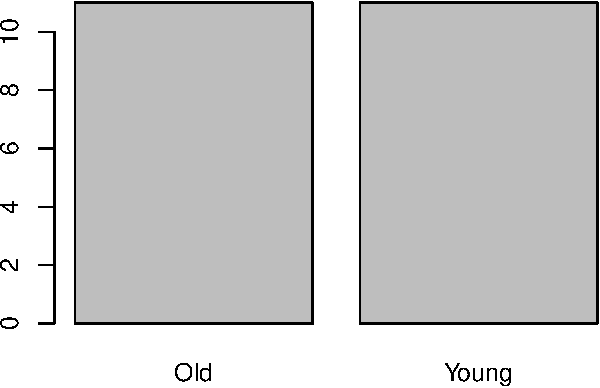
\includegraphics[width=0.5\linewidth]{Rcourse_files/figure-latex/barplot-1}

\hypertarget{visualizing-bivariate-categorical-data}{%
\subsubsection{Visualizing Bivariate Categorical Data}\label{visualizing-bivariate-categorical-data}}

There are several generalizations of the barplot, aimed to deal with the visualization of bivariate categorical data.
They are sometimes known as the \emph{clustered bar plot} and the \emph{stacked bar plot}.
In this text, we advocate the use of the \emph{mosaic plot} which is also the default in R.

\begin{Shaded}
\begin{Highlighting}[]
\KeywordTok{plot}\NormalTok{(table1, }\DataTypeTok{main=}\StringTok{'Bivariate mosaic plot'}\NormalTok{)}
\end{Highlighting}
\end{Shaded}

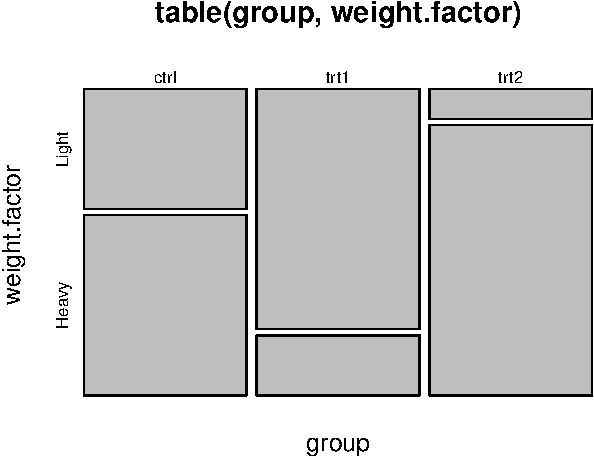
\includegraphics[width=0.5\linewidth]{Rcourse_files/figure-latex/unnamed-chunk-129-1}

Things to note:

\begin{itemize}
\tightlist
\item
  The proportion of each category is encoded in the width of the bars (more girls than boys here)
\item
  Zero observations are marked as a line.
\end{itemize}

\hypertarget{visualizing-multivariate-categorical-data}{%
\subsubsection{Visualizing Multivariate Categorical Data}\label{visualizing-multivariate-categorical-data}}

The \emph{mosaic plot} is not easy to generalize to more than two variables, but it is still possible (at the cost of interpretability).

\begin{Shaded}
\begin{Highlighting}[]
\KeywordTok{plot}\NormalTok{(table2}\FloatTok{.1}\NormalTok{, }\DataTypeTok{main=}\StringTok{'Trivaraite mosaic plot'}\NormalTok{)}
\end{Highlighting}
\end{Shaded}

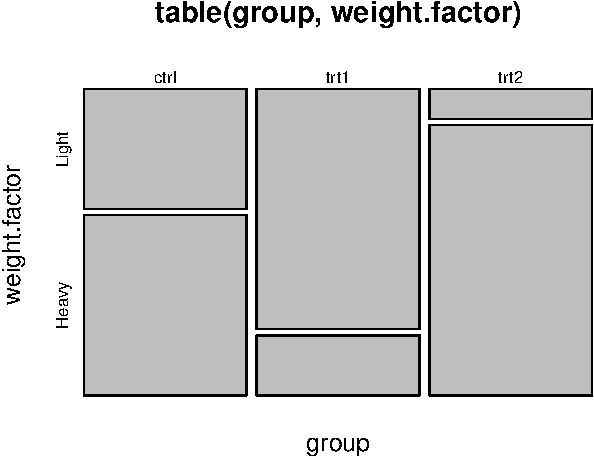
\includegraphics[width=0.5\linewidth]{Rcourse_files/figure-latex/unnamed-chunk-130-1}

When one of the variables is a (discrete) time variable, then the plot has a notion dynamics in time. For this see the Alluvial plot \ref{alluvial}.

If the variables represent a hierarchy, consider a \textbf{Sunburst Plot}:

\begin{Shaded}
\begin{Highlighting}[]
\KeywordTok{library}\NormalTok{(sunburstR)}
\CommentTok{# read in sample visit-sequences.csv data provided in source}
\CommentTok{# https://gist.github.com/kerryrodden/7090426#file-visit-sequences-csv}
\NormalTok{sequences <-}\StringTok{ }\KeywordTok{read.csv}\NormalTok{(}
  \KeywordTok{system.file}\NormalTok{(}\StringTok{"examples/visit-sequences.csv"}\NormalTok{,}\DataTypeTok{package=}\StringTok{"sunburstR"}\NormalTok{)}
\NormalTok{  ,}\DataTypeTok{header=}\NormalTok{F}
\NormalTok{  ,}\DataTypeTok{stringsAsFactors =} \OtherTok{FALSE}
\NormalTok{)}
\KeywordTok{sunburst}\NormalTok{(sequences) }\CommentTok{# In the HTML version of the book this plot is interactive.}
\end{Highlighting}
\end{Shaded}

\includegraphics[width=0.5\linewidth]{Rcourse_files/figure-latex/sunburst-1}

\hypertarget{continuous-data}{%
\subsection{Continuous Data}\label{continuous-data}}

\hypertarget{visualizing-univariate-continuous-data}{%
\subsubsection{Visualizing Univariate Continuous Data}\label{visualizing-univariate-continuous-data}}

Unlike categorical variables, there are endlessly many ways to visualize continuous variables.
The simplest way is to look at the raw data via the \texttt{stripchart}.

\begin{Shaded}
\begin{Highlighting}[]
\NormalTok{sample1 <-}\StringTok{ }\KeywordTok{rexp}\NormalTok{(}\DecValTok{10}\NormalTok{)                             }
\KeywordTok{stripchart}\NormalTok{(sample1)}
\end{Highlighting}
\end{Shaded}

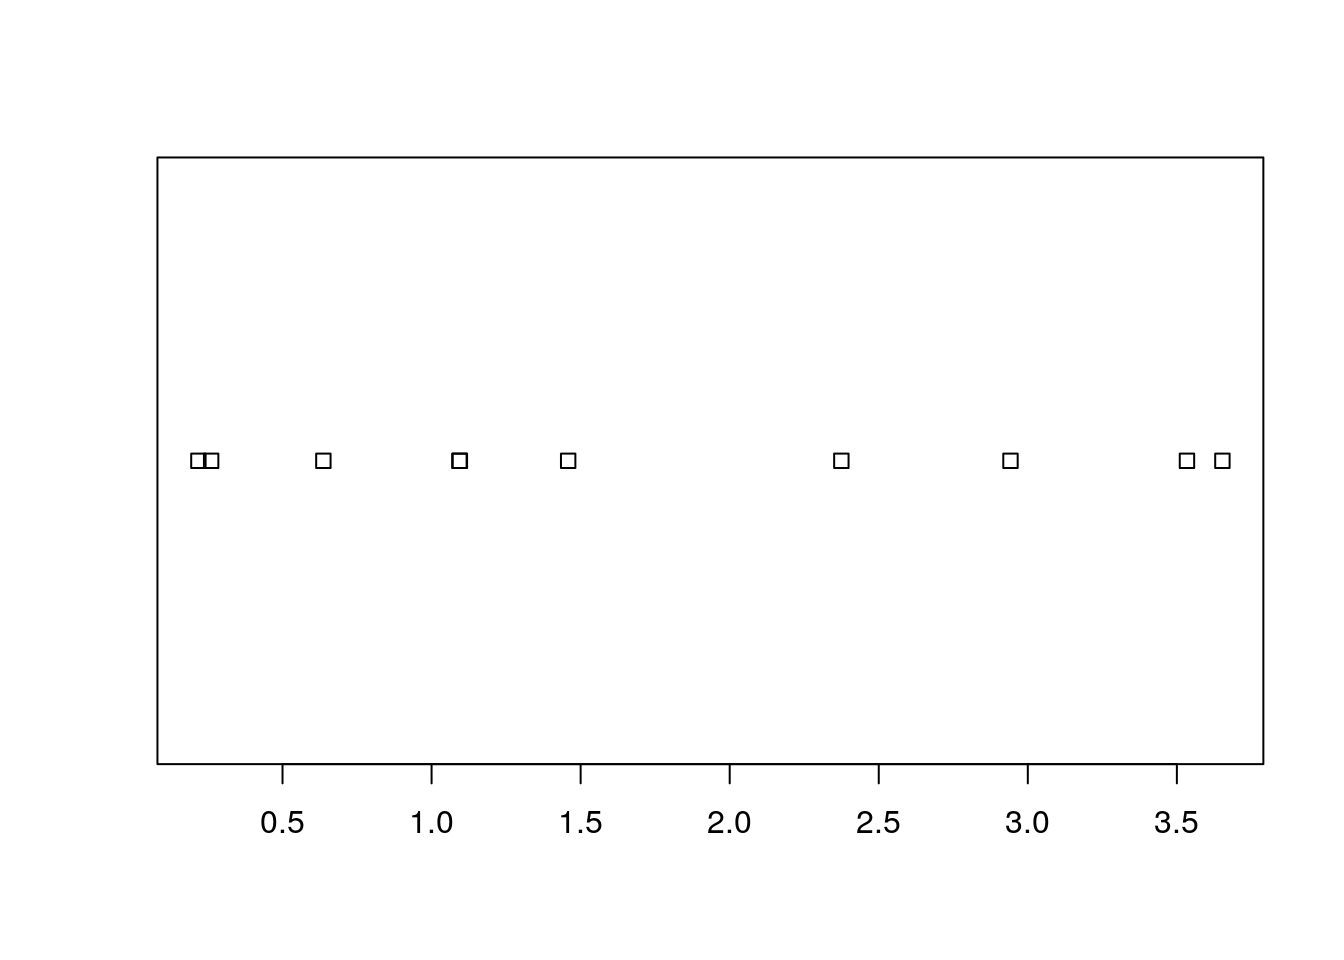
\includegraphics[width=0.5\linewidth]{Rcourse_files/figure-latex/unnamed-chunk-131-1}

Clearly, if there are many observations, the \texttt{stripchart} will be a useless line of black dots.
We thus bin them together, and look at the frequency of each bin; this is the \emph{histogram}.
R's \texttt{histogram} function has very good defaults to choose the number of bins.
Here is a histogram showing the counts of each bin.

\begin{Shaded}
\begin{Highlighting}[]
\NormalTok{sample1 <-}\StringTok{ }\KeywordTok{rexp}\NormalTok{(}\DecValTok{100}\NormalTok{)                            }
\KeywordTok{hist}\NormalTok{(sample1, }\DataTypeTok{freq=}\NormalTok{T, }\DataTypeTok{main=}\StringTok{'Counts'}\NormalTok{)        }
\end{Highlighting}
\end{Shaded}

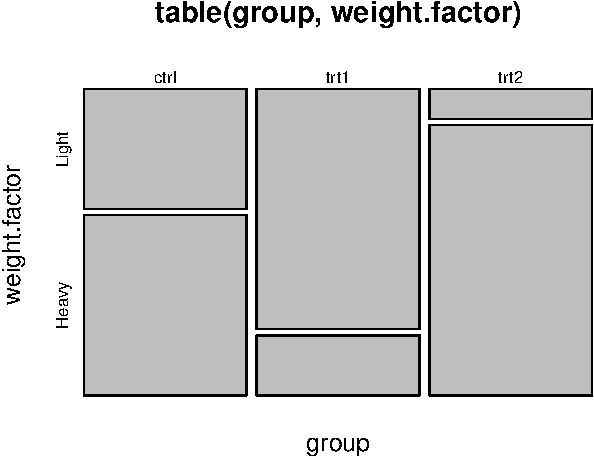
\includegraphics[width=0.5\linewidth]{Rcourse_files/figure-latex/unnamed-chunk-132-1}

The bin counts can be replaced with the proportion of each bin using the \texttt{freq} argument.

\begin{Shaded}
\begin{Highlighting}[]
\KeywordTok{hist}\NormalTok{(sample1, }\DataTypeTok{freq=}\NormalTok{F, }\DataTypeTok{main=}\StringTok{'Proportion'}\NormalTok{)    }
\end{Highlighting}
\end{Shaded}

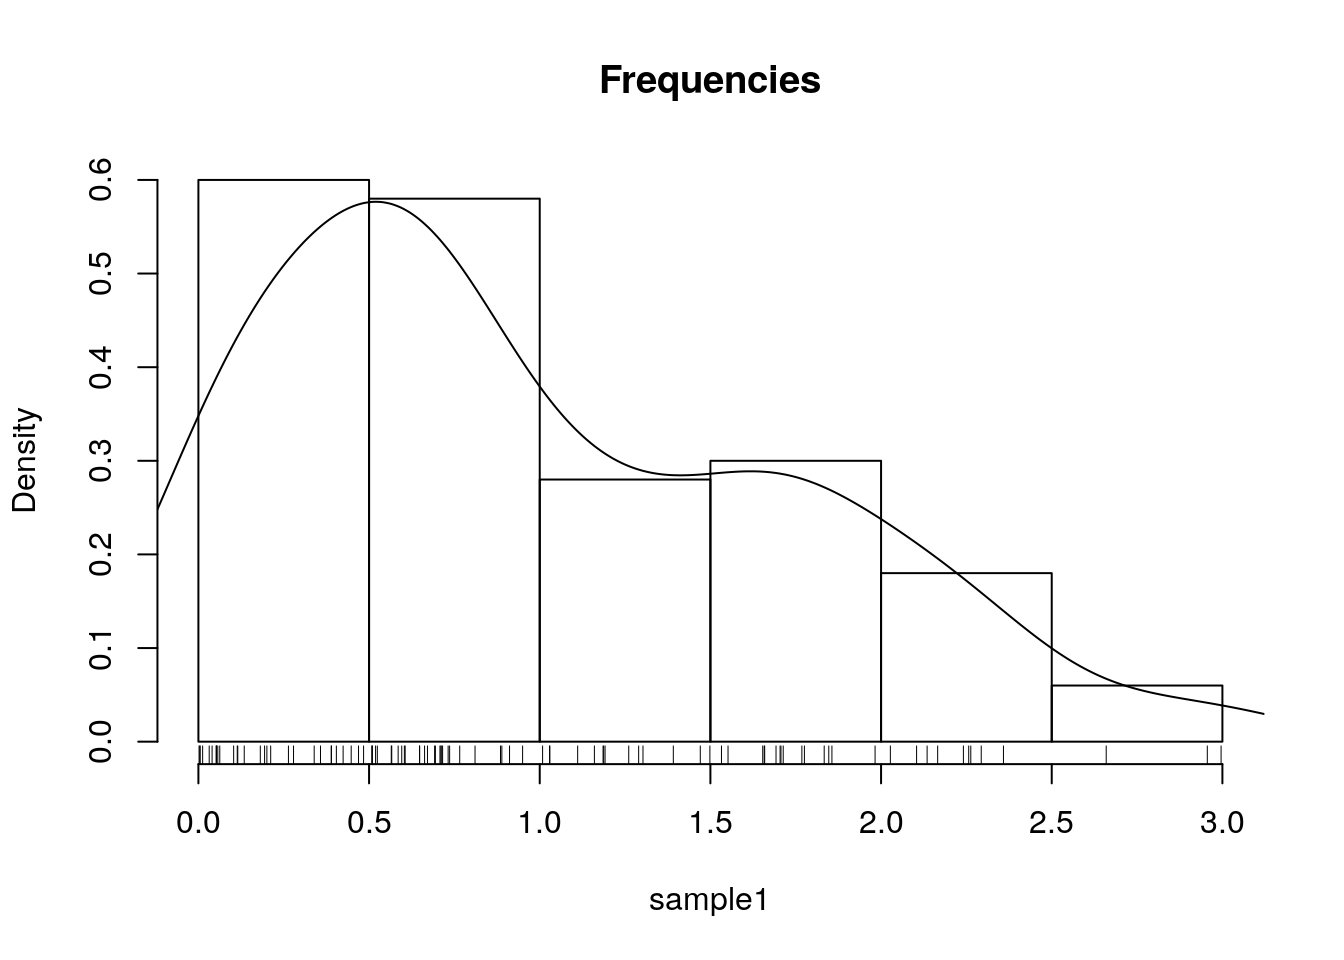
\includegraphics[width=0.5\linewidth]{Rcourse_files/figure-latex/unnamed-chunk-133-1}

Things to note:

\begin{itemize}
\tightlist
\item
  The bins' proportion summary is larger than 1 because it considers each bin's width, which in this case has a constant width of 0.5, hence the total proportion sum is 1/0.5=2.
\end{itemize}

The bins of a histogram are non overlapping.
We can adopt a sliding window approach, instead of binning.
This is the \emph{density plot} which is produced with the \texttt{density} function, and added to an existing plot with the \texttt{lines} function.
The \texttt{rug} function adds the original data points as ticks on the axes, and is strongly recommended to detect artifacts introduced by the binning of the histogram, or the smoothing of the density plot.

\begin{Shaded}
\begin{Highlighting}[]
\KeywordTok{hist}\NormalTok{(sample1, }\DataTypeTok{freq=}\NormalTok{F, }\DataTypeTok{main=}\StringTok{'Frequencies'}\NormalTok{)   }
\KeywordTok{lines}\NormalTok{(}\KeywordTok{density}\NormalTok{(sample1))                     }
\KeywordTok{rug}\NormalTok{(sample1)}
\end{Highlighting}
\end{Shaded}

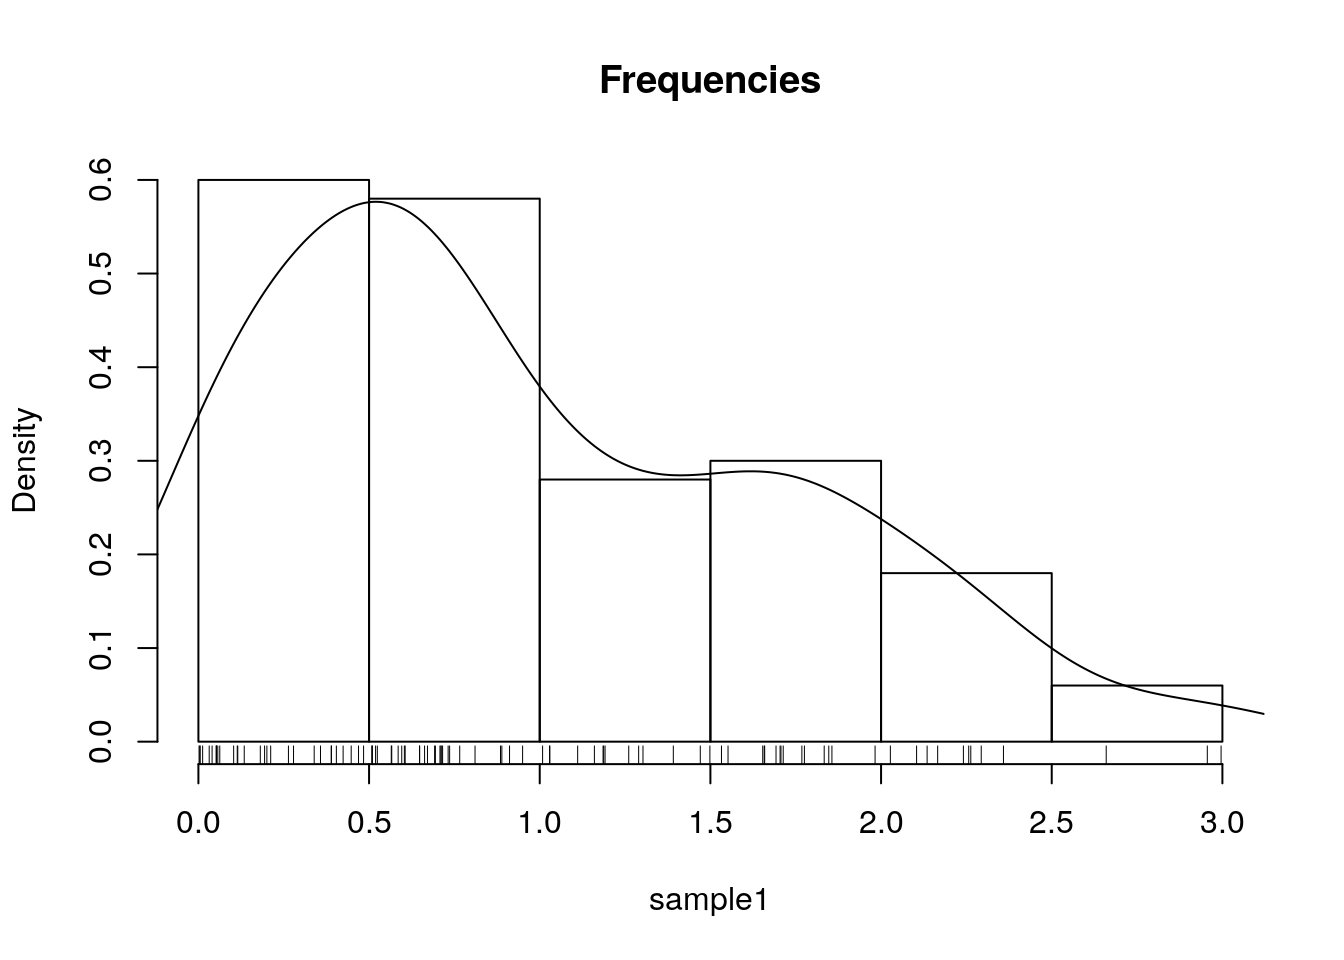
\includegraphics[width=0.5\linewidth]{Rcourse_files/figure-latex/unnamed-chunk-134-1}

\BeginKnitrBlock{remark}
\iffalse{} {Remark. } \fi{}Why would it make no sense to make a table, or a barplot, of continuous data?
\EndKnitrBlock{remark}

One particularly useful visualization, due to John W. Tukey, is the \emph{boxplot}.
The boxplot is designed to capture the main phenomena in the data, and simultaneously point to outlines.

\begin{Shaded}
\begin{Highlighting}[]
\KeywordTok{boxplot}\NormalTok{(sample1)    }
\end{Highlighting}
\end{Shaded}

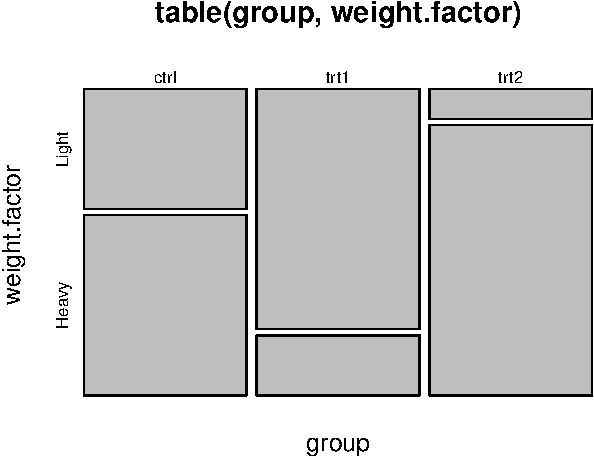
\includegraphics[width=0.5\linewidth]{Rcourse_files/figure-latex/unnamed-chunk-136-1}

Another way to deal with a massive amount of data points, is to emphasize important points, and conceal non-important.
This is the purpose of \textbf{circle-packing} (example from \href{https://www.r-graph-gallery.com/308-interactive-circle-packing/}{r-graph gallery}):

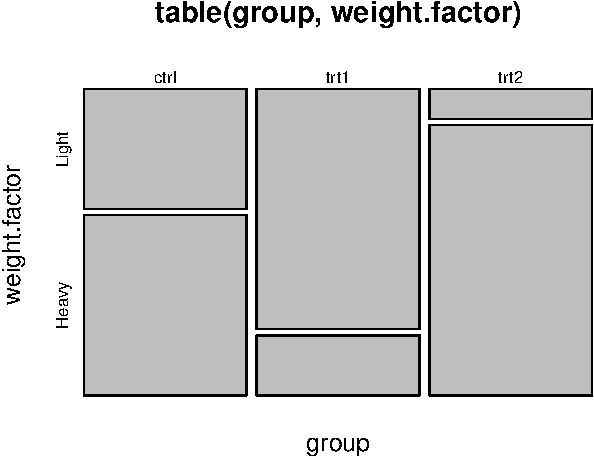
\includegraphics[width=0.5\linewidth]{Rcourse_files/figure-latex/unnamed-chunk-137-1}

\hypertarget{visualizing-bivariate-continuous-data}{%
\subsubsection{Visualizing Bivariate Continuous Data}\label{visualizing-bivariate-continuous-data}}

The bivariate counterpart of the \texttt{stipchart} is the celebrated scatter plot.

\begin{Shaded}
\begin{Highlighting}[]
\NormalTok{n <-}\StringTok{ }\DecValTok{20}
\NormalTok{x1 <-}\StringTok{ }\KeywordTok{rexp}\NormalTok{(n)}
\NormalTok{x2 <-}\StringTok{ }\DecValTok{2}\OperatorTok{*}\StringTok{ }\NormalTok{x1 }\OperatorTok{+}\StringTok{ }\DecValTok{4} \OperatorTok{+}\StringTok{ }\KeywordTok{rexp}\NormalTok{(n)}
\KeywordTok{plot}\NormalTok{(x2}\OperatorTok{~}\NormalTok{x1)}
\end{Highlighting}
\end{Shaded}

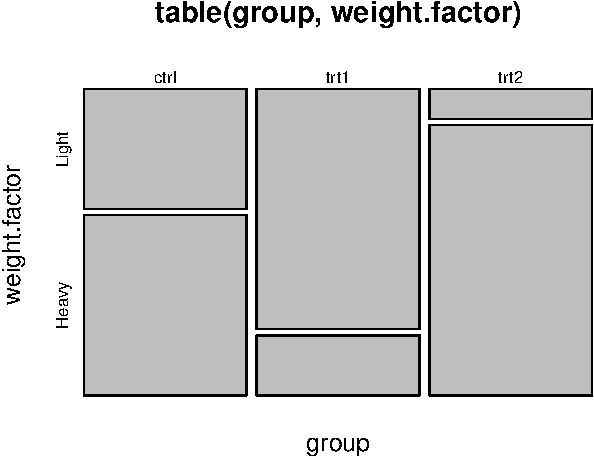
\includegraphics[width=0.5\linewidth]{Rcourse_files/figure-latex/unnamed-chunk-138-1}

A scatter-plot may be augmented with marginal univariate visualization.
See, for instance, the \emph{rug} function to add the raw data on the margins:

\begin{Shaded}
\begin{Highlighting}[]
\KeywordTok{plot}\NormalTok{(x2}\OperatorTok{~}\NormalTok{x1)}
\KeywordTok{rug}\NormalTok{(x1,}\DataTypeTok{side =} \DecValTok{1}\NormalTok{)}
\KeywordTok{rug}\NormalTok{(x2,}\DataTypeTok{side =} \DecValTok{2}\NormalTok{)}
\end{Highlighting}
\end{Shaded}

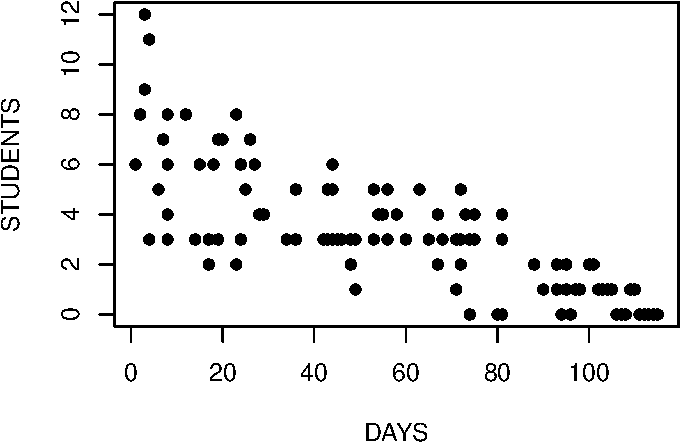
\includegraphics[width=0.5\linewidth]{Rcourse_files/figure-latex/unnamed-chunk-139-1}

A fancier version may use a histogram on the margins:

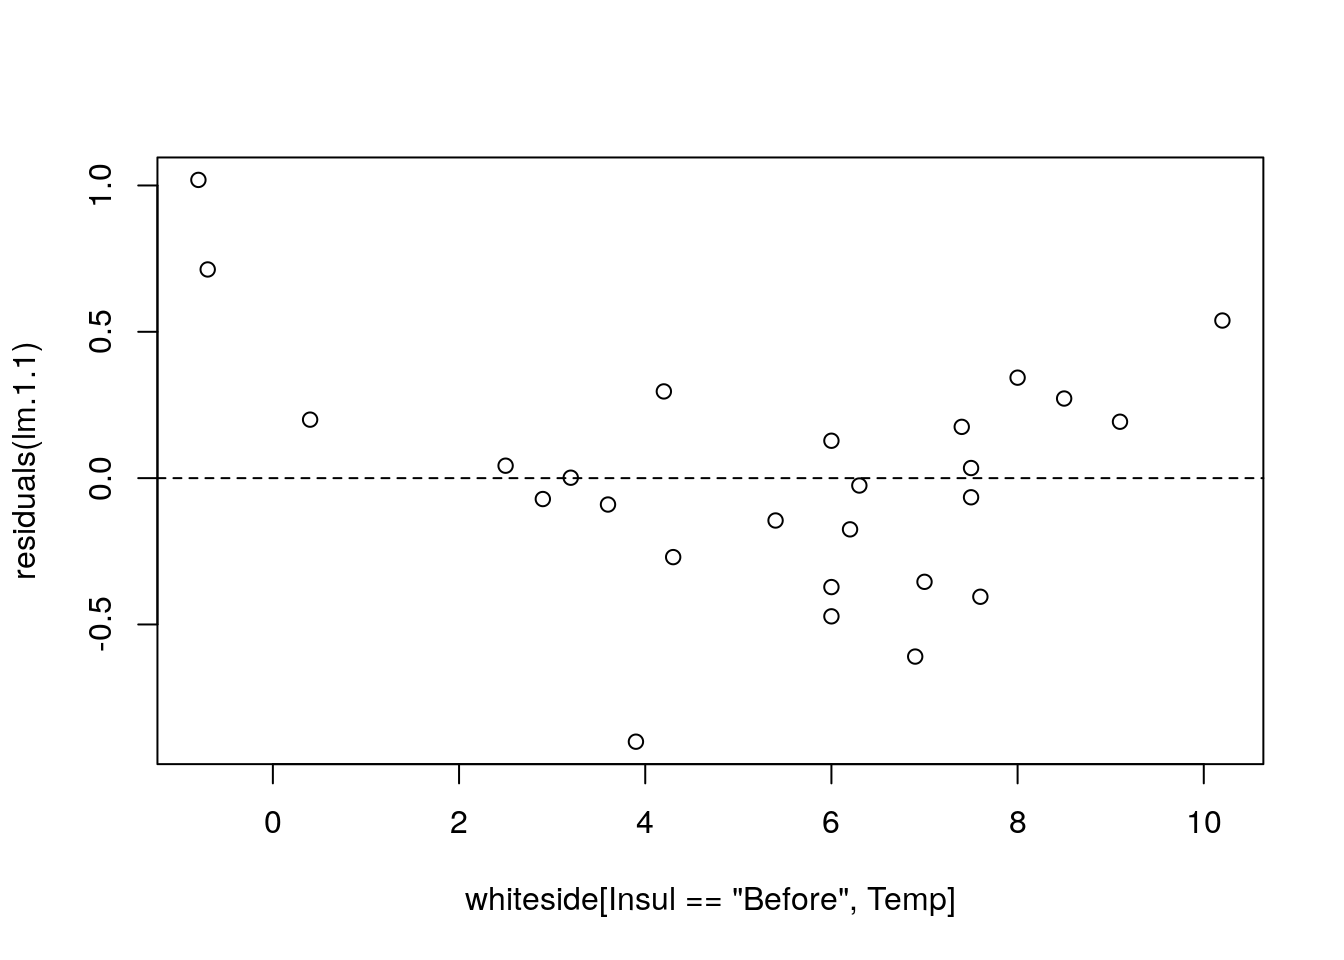
\includegraphics[width=0.5\linewidth]{Rcourse_files/figure-latex/unnamed-chunk-140-1}

Like the univariate \texttt{stripchart}, the scatter plot will be an uninformative mess in the presence of a lot of data.
A nice bivariate counterpart of the univariate histogram is the \emph{hexbin plot}, which tessellates the plane with hexagons, and reports their frequencies.

\begin{Shaded}
\begin{Highlighting}[]
\KeywordTok{library}\NormalTok{(hexbin) }\CommentTok{# load required library}
\NormalTok{n <-}\StringTok{ }\FloatTok{2e5}
\NormalTok{x1 <-}\StringTok{ }\KeywordTok{rexp}\NormalTok{(n)}
\NormalTok{x2 <-}\StringTok{ }\DecValTok{2}\OperatorTok{*}\StringTok{ }\NormalTok{x1 }\OperatorTok{+}\StringTok{ }\DecValTok{4} \OperatorTok{+}\StringTok{ }\KeywordTok{rnorm}\NormalTok{(n)}
\KeywordTok{plot}\NormalTok{(}\KeywordTok{hexbin}\NormalTok{(}\DataTypeTok{x =}\NormalTok{ x1, }\DataTypeTok{y =}\NormalTok{ x2))}
\end{Highlighting}
\end{Shaded}

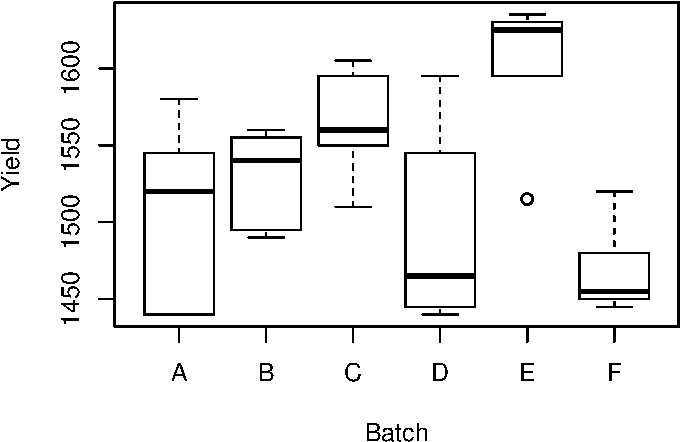
\includegraphics[width=0.5\linewidth]{Rcourse_files/figure-latex/unnamed-chunk-141-1}

\hypertarget{visualizing-multivariate-continuous-data}{%
\subsubsection{Visualizing Multivariate Continuous Data}\label{visualizing-multivariate-continuous-data}}

Visualizing multivariate data is a tremendous challenge given that we cannot grasp \(4\) dimensional spaces, nor can the computer screen present more than \(2\) dimensional spaces.
We thus have several options:
(i) To project the data to 2D. This is discussed in the Dimensionality Reduction Section \ref{dim-reduce}.
(ii) To visualize not the raw data, but rather its summaries, like the covariance matrix.

Our own \href{https://github.com/EfratVil/MultiNav}{Multinav} package adopts an interactive approach.
For each (multivariate) observation a simple univariate summary may be computed and visualized.
These summaries may be compared, and the original (multivariate) observation inspected upon demand.
Contact \href{http://efratvil.github.io/home/index.html}{Efrat} for more details.\\
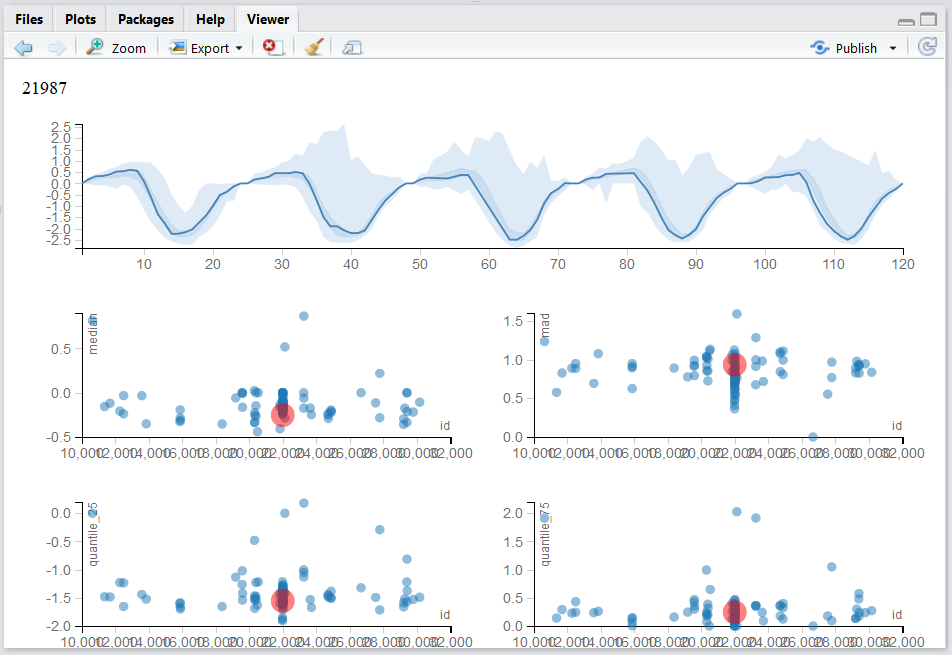
\includegraphics{art/multinav.png}

An alternative approach starts with the covariance matrix, \(\hat \Sigma\), that can be visualized as an image.
Note the use of the \texttt{::} operator (called \emph{Double Colon Operator}, for help: \texttt{?\textquotesingle{}::\textquotesingle{}}), which is used to call a function from some package, without loading the whole package.
We will use the \texttt{::} operator when we want to emphasize the package of origin of a function.

\begin{Shaded}
\begin{Highlighting}[]
\NormalTok{covariance <-}\StringTok{ }\KeywordTok{cov}\NormalTok{(longley) }\CommentTok{# The covariance of the longley dataset}
\NormalTok{correlations <-}\StringTok{ }\KeywordTok{cor}\NormalTok{(longley) }\CommentTok{# The correlations of the longley dataset}
\NormalTok{lattice}\OperatorTok{::}\KeywordTok{levelplot}\NormalTok{(correlations)}
\end{Highlighting}
\end{Shaded}

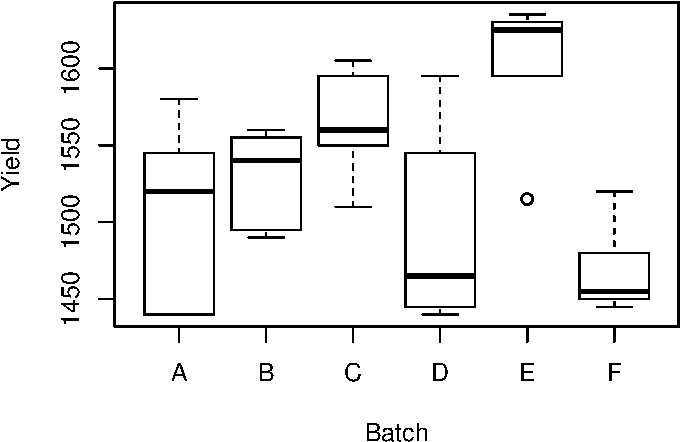
\includegraphics[width=0.5\linewidth]{Rcourse_files/figure-latex/unnamed-chunk-142-1}

If we believe the covariance has some structure, we can do better than viewing the raw correlations.
In temporal, and spatial data, we believe correlations decay as some function of distances.
We can thus view correlations as a function of the distance between observations. This is known as a \emph{variogram}.
Note that for a variogram to be informative, it is implied that correlations are merely a function of distances (and not locations themselves).
This is formally known as \emph{stationary} and \emph{isotropic} correlations.

\begin{figure}
\centering
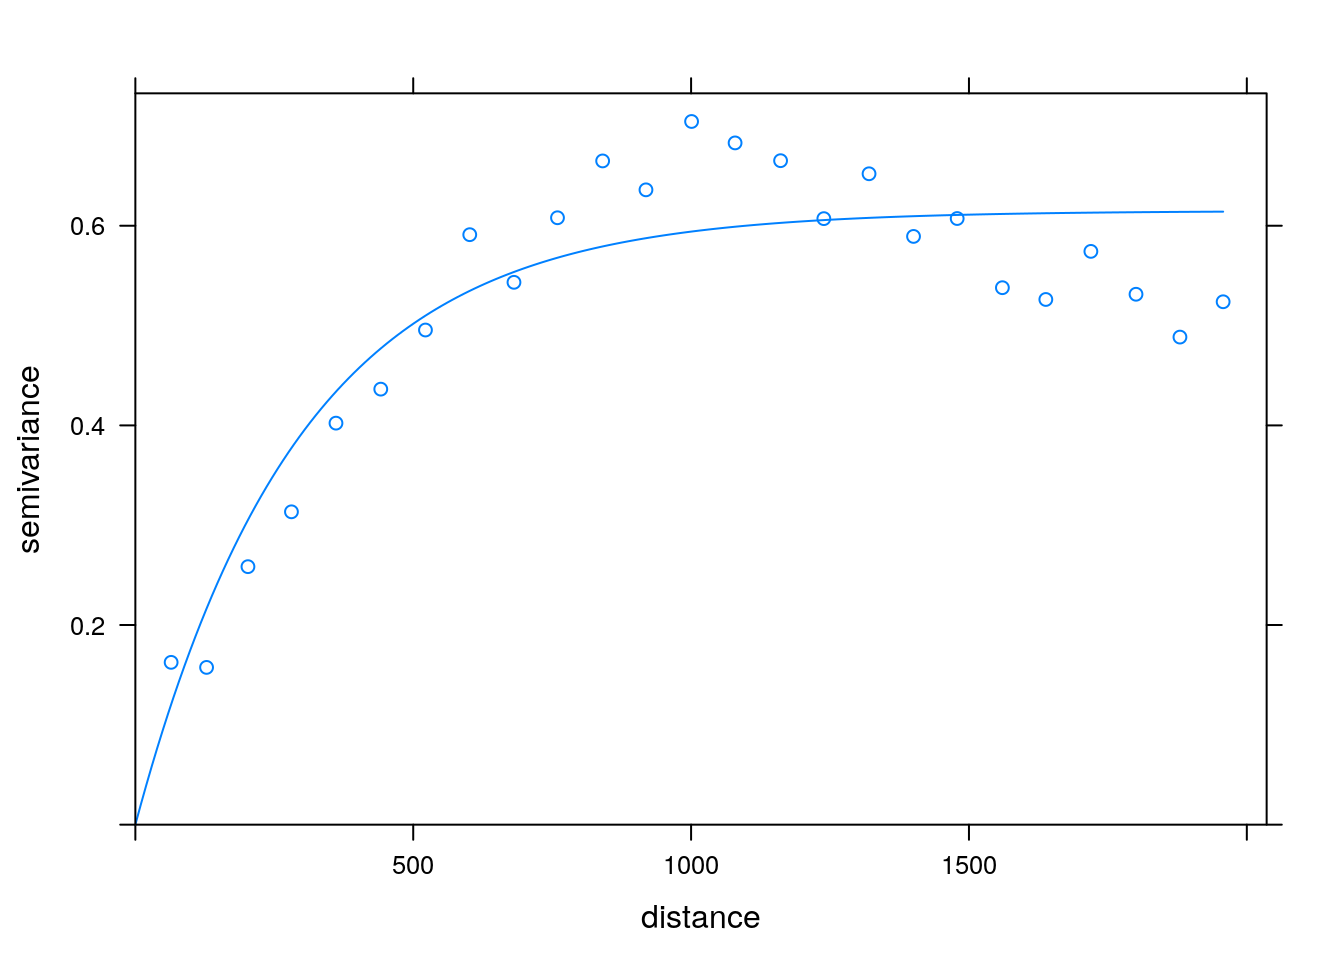
\includegraphics{art/variogram.png}
\caption{Variogram: plotting correlation as a function of spatial distance. Courtesy of Ron Sarafian.}
\end{figure}

\hypertarget{parcoord}{%
\subsubsection{Parallel Coordinate Plots}\label{parcoord}}

In a parallel coordinate plot, we plot a multivariate observation as a function of its coordinates.
In the following example, we visualize the celebrated \href{https://en.wikipedia.org/wiki/Iris_flower_data_set}{Iris dataset}.
In this dataset, for each of 50 iris flowers, Edgar Anderson measured 4 characteristics.

\begin{Shaded}
\begin{Highlighting}[]
\NormalTok{ir <-}\StringTok{ }\KeywordTok{rbind}\NormalTok{(iris3[,,}\DecValTok{1}\NormalTok{], iris3[,,}\DecValTok{2}\NormalTok{], iris3[,,}\DecValTok{3}\NormalTok{])}
\NormalTok{MASS}\OperatorTok{::}\KeywordTok{parcoord}\NormalTok{(}\KeywordTok{log}\NormalTok{(ir)[, }\KeywordTok{c}\NormalTok{(}\DecValTok{3}\NormalTok{, }\DecValTok{4}\NormalTok{, }\DecValTok{2}\NormalTok{, }\DecValTok{1}\NormalTok{)], }\DataTypeTok{col =} \DecValTok{1} \OperatorTok{+}\StringTok{ }\NormalTok{(}\DecValTok{0}\OperatorTok{:}\DecValTok{149}\NormalTok{)}\OperatorTok\DecValTok{50}\NormalTok{)}
\end{Highlighting}
\end{Shaded}

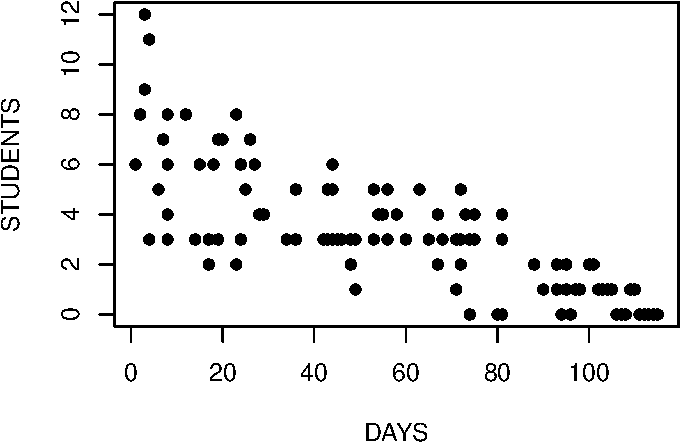
\includegraphics[width=0.5\linewidth]{Rcourse_files/figure-latex/unnamed-chunk-143-1}

\hypertarget{mixed-type-data}{%
\section{Mixed Type Data}\label{mixed-type-data}}

Most real data sets will be of mixed type: both categorical and continuous.
One approach to view such data, is to visualize the continuous variables separately, for each level of the categorical variables.
There are, however, interesting dedicated visualization for such data.

\hypertarget{alluvial}{%
\subsection{Alluvial Diagram}\label{alluvial}}

An Alluvial plot is a type of \protect\hyperlink{parcoord}{Parallel Coordinate Plot} for multivariate categorical data.
It is particularly interesting when the \(x\) axis is a discretized time variable, and it is used to visualize flow.

The following example, from the \textbf{ggalluvial} package Vignette by \href{https://cran.r-project.org/web/packages/ggalluvial/vignettes/ggalluvial.html}{Jason Cory Brunson}, demonstrates the flow of students between different majors, as semesters evolve.

\begin{Shaded}
\begin{Highlighting}[]
\KeywordTok{library}\NormalTok{(ggalluvial)}
\KeywordTok{data}\NormalTok{(majors)}
\NormalTok{majors}\OperatorTok{$}\NormalTok{curriculum <-}\StringTok{ }\KeywordTok{as.factor}\NormalTok{(majors}\OperatorTok{$}\NormalTok{curriculum)}
\KeywordTok{ggplot}\NormalTok{(majors,}
       \KeywordTok{aes}\NormalTok{(}\DataTypeTok{x =}\NormalTok{ semester, }\DataTypeTok{stratum =}\NormalTok{ curriculum, }\DataTypeTok{alluvium =}\NormalTok{ student,}
           \DataTypeTok{fill =}\NormalTok{ curriculum, }\DataTypeTok{label =}\NormalTok{ curriculum)) }\OperatorTok{+}
\StringTok{  }\KeywordTok{scale_fill_brewer}\NormalTok{(}\DataTypeTok{type =} \StringTok{"qual"}\NormalTok{, }\DataTypeTok{palette =} \StringTok{"Set2"}\NormalTok{) }\OperatorTok{+}
\StringTok{  }\KeywordTok{geom_flow}\NormalTok{(}\DataTypeTok{stat =} \StringTok{"alluvium"}\NormalTok{, }\DataTypeTok{lode.guidance =} \StringTok{"rightleft"}\NormalTok{,}
            \DataTypeTok{color =} \StringTok{"darkgray"}\NormalTok{) }\OperatorTok{+}
\StringTok{  }\KeywordTok{geom_stratum}\NormalTok{() }\OperatorTok{+}
\StringTok{  }\KeywordTok{theme}\NormalTok{(}\DataTypeTok{legend.position =} \StringTok{"bottom"}\NormalTok{) }\OperatorTok{+}
\StringTok{  }\KeywordTok{ggtitle}\NormalTok{(}\StringTok{"student curricula across several semesters"}\NormalTok{)}
\end{Highlighting}
\end{Shaded}

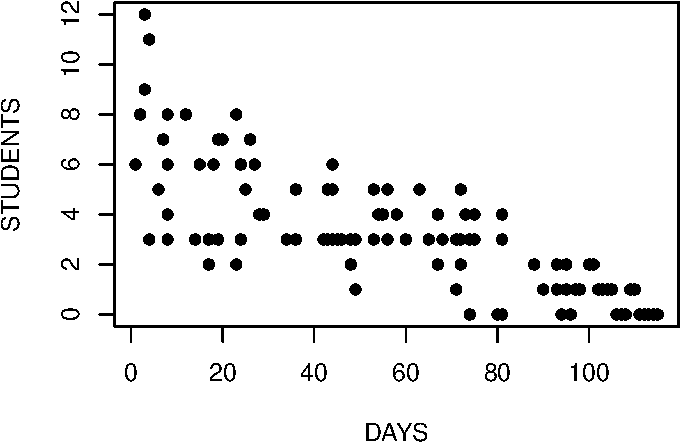
\includegraphics[width=0.5\linewidth]{Rcourse_files/figure-latex/unnamed-chunk-144-1}

Things to note:

\begin{itemize}
\tightlist
\item
  We used the \textbf{ggalluvial} package of the \textbf{ggplot2} ecosystem. More on \textbf{ggplot2} in the \protect\hyperlink{plotting}{Plotting Chapter}.
\item
  Time is on the \(x\) axis. Categories are color coded.
\end{itemize}

\BeginKnitrBlock{remark}
\iffalse{} {Remark. } \fi{}If the width of the lines encode magnitude, the plot is also called a Sankey diagram.
\EndKnitrBlock{remark}

\hypertarget{bibliographic-notes-3}{%
\section{Bibliographic Notes}\label{bibliographic-notes-3}}

Like any other topic in this book, you can consult \citet{venables2013modern}.
The seminal book on EDA, written long before R was around, is \citet{tukey1977exploratory}.
For an excellent text on robust statistics see \citet{wilcox2011introduction}.

\hypertarget{practice-yourself-2}{%
\section{Practice Yourself}\label{practice-yourself-2}}

\begin{enumerate}
\def\labelenumi{\arabic{enumi}.}
\item
  Read about the Titanic data set using \texttt{?Titanic}. Inspect it with the \texttt{table} and with the \texttt{ftable} commands. Which do you prefer?
\item
  Inspect the Titanic data with a plot. Start with \texttt{plot(Titanic)} Try also \texttt{lattice::dotplot}. Which is the passenger category with most survivors? Which plot do you prefer? Which scales better to more categories?
\item
  Read about the women data using \texttt{?women}.

  \begin{enumerate}
  \def\labelenumii{\arabic{enumii}.}
  \tightlist
  \item
    Compute the average of each variable. What is the average of the heights?
  \item
    Plot a histogram of the heights. Add ticks using \texttt{rug}.
  \item
    Plot a boxplot of the weights.
  \item
    Plot the heights and weights using a scatter plot. Add ticks using \texttt{rug}.
  \end{enumerate}
\item
  Choose \(\alpha\) to define a new symmetry measure: \(1/2(x_\alpha+x_{1-\alpha})-x_{0.5}\).
  Write a function that computes it, and apply it on women's heights data.
\item
  Compute the covariance matrix of women's heights and weights. Compute the correlation matrix. View the correlation matrix as an image using \texttt{lattice::levelplot}.
\item
  Pick a dataset with two LONG continous variables from \texttt{?datasets}. Plot it using \texttt{hexbin::hexbin}.
\end{enumerate}

\hypertarget{lm}{%
\chapter{Linear Models}\label{lm}}

\hypertarget{problem-setup}{%
\section{Problem Setup}\label{problem-setup}}

\BeginKnitrBlock{example}[Bottle Cap Production]
\protect\hypertarget{exm:cap-experiment}{}{\label{exm:cap-experiment} \iffalse (Bottle Cap Production) \fi{} }Consider a randomized experiment designed to study the effects of temperature and pressure on the diameter of manufactured a bottle cap.
\EndKnitrBlock{example}

\BeginKnitrBlock{example}[Rental Prices]
\protect\hypertarget{exm:rental}{}{\label{exm:rental} \iffalse (Rental Prices) \fi{} }Consider the prediction of rental prices given an appartment's attributes.
\EndKnitrBlock{example}

Both examples require some statistical model, but they are very different.
The first is a \emph{causal inference} problem: we want to design an intervention so that we need to recover the causal effect of temperature and pressure.
The second is a \href{https://en.wikipedia.org/wiki/Prediction}{prediction} problem, a.k.a. a \href{https://en.wikipedia.org/wiki/Forecasting}{forecasting} problem, in which we don't care about the causal effects, we just want good predictions.

In this chapter we discuss the causal problem in Example \ref{exm:cap-experiment}.
This means that when we assume a model, we assume it is the actual \emph{data generating process}, i.e., we assume the \emph{sampling distribution} is well specified.
In the econometric literature, these are the \href{https://en.wikipedia.org/wiki/Structural_equation_modeling}{structural equations}.
The second type of problems is discussed in the Supervised Learning Chapter \ref{supervised}.

Here are some more examples of the types of problems we are discussing.

\BeginKnitrBlock{example}[Plant Growth]
\protect\hypertarget{exm:unnamed-chunk-146}{}{\label{exm:unnamed-chunk-146} \iffalse (Plant Growth) \fi{} }Consider the treatment of various plants with various fertilizers to study the fertilizer's effect on growth.
\EndKnitrBlock{example}

\BeginKnitrBlock{example}[Return to Education]
\protect\hypertarget{exm:unnamed-chunk-147}{}{\label{exm:unnamed-chunk-147} \iffalse (Return to Education) \fi{} }Consider the study of return to education by analyzing the incomes of individuals with different education years.
\EndKnitrBlock{example}

\BeginKnitrBlock{example}[Drug Effect]
\protect\hypertarget{exm:unnamed-chunk-148}{}{\label{exm:unnamed-chunk-148} \iffalse (Drug Effect) \fi{} }Consider the study of the effect of a new drug for hemophilia, by analyzing the level of blood coagulation after the administration of various amounts of the new drug.
\EndKnitrBlock{example}

Let's present the linear model.
We assume that a response\footnote{The ``response'' is also known as the ``dependent'' variable in the statistical literature, or the ``labels'' in the machine learning literature.} variable is the sum of effects of some factors\footnote{The ``factors'' are also known as the ``independent variable'', or ``the design'', in the statistical literature, and the ``features'', or ``attributes'' in the machine learning literature.}.
Denoting the response variable by \(y\), the factors by \(x=(x_1,\dots,x_p)\), and the effects by \(\beta:=(\beta_1,\dots,\beta_p)\) the linear model assumption implies that the expected response is the sum of the factors effects:

\begin{align}
  E[y]=x_1 \beta_1 + \dots + x_p \beta_p = \sum_{j=1}^p x_j \beta_j = x'\beta .
  \label{eq:linear-mean}
\end{align}
Clearly, there may be other factors that affect the the caps' diameters.
We thus introduce an error term\footnote{The ``error term'' is also known as the ``noise'', or the ``common causes of variability''.}, denoted by \(\varepsilon\), to capture the effects of all unmodeled factors and measurement error\footnote{You may philosophize if the measurement error is a mere instance of unmodeled factors or not, but this has no real implication for our purposes.}.
The implied generative process of a sample of \(i=1,\dots,n\) observations it thus
\begin{align}
  y_i = x_i'\beta + \varepsilon_i = \sum_j x_{i,j} \beta_j + \varepsilon_i , i=1,\dots,n .
  \label{eq:linear-observed}
\end{align}
or in matrix notation
\begin{align}
  y = X \beta + \varepsilon .
  \label{eq:linear-matrix}
\end{align}

Let's demonstrate Eq.\eqref{eq:linear-observed}.
In our bottle-caps example {[}\ref{exm:cap-experiment}{]}, we may produce bottle caps at various temperatures.
We design an experiment where we produce bottle-caps at varying temperatures.
Let \(x_i\) be the temperature at which bottle-cap \(i\) was manufactured.
Let \(y_i\) be its measured diameter.
By the linear model assumption, the expected diameter varies linearly with the temperature: \(\mathbb{E}[y_i]=\beta_0 + x_i \beta_1\).
This implies that \(\beta_1\) is the (expected) change in diameter due to a unit change in temperature.

\BeginKnitrBlock{remark}
\iffalse{} {Remark. } \fi{}In \href{https://en.wikipedia.org/wiki/Regression_toward_the_mean}{Galton's} classical regression problem, where we try to seek the relation between the heights of sons and fathers then \(p=1\), \(y_i\) is the height of the \(i\)'th father, and \(x_i\) the height of the \(i\)'th son.
This is a prediction problem, more than it is a causal-inference problem.
\EndKnitrBlock{remark}

There are many reasons linear models are very popular:

\begin{enumerate}
\def\labelenumi{\arabic{enumi}.}
\item
  Before the computer age, these were pretty much the only models that could actually be computed\footnote{By ``computed'' we mean what statisticians call ``fitted'', or ``estimated'', and computer scientists call ``learned''.}.
  The whole Analysis of Variance (ANOVA) literature is an instance of linear models, that relies on sums of squares, which do not require a computer to work with.
\item
  For purposes of prediction, where the actual data generating process is not of primary importance, they are popular because they simply work.
  Why is that?
  They are simple so that they do not require a lot of data to be computed.
  Put differently, they may be biased, but their variance is small enough to make them more accurate than other models.
\item
  For non continuous predictors, \textbf{any} functional relation can be cast as a linear model.
\item
  For the purpose of \emph{screening}, where we only want to show the existence of an effect, and are less interested in the magnitude of that effect, a linear model is enough.
\item
  If the true generative relation is not linear, but smooth enough, then the linear function is a good approximation via Taylor's theorem.
\end{enumerate}

There are still two matters we have to attend:
(i) How to estimate \(\beta\)?
(ii) How to perform inference?

In the simplest linear models the estimation of \(\beta\) is done using the method of least squares. A linear model with least squares estimation is known as Ordinary Least Squares (OLS).
The OLS problem:

\begin{align}
  \hat \beta:= argmin_\beta \{ \sum_i (y_i-x_i'\beta)^2 \},
  \label{eq:ols}
\end{align}
and in matrix notation
\begin{align}
  \hat \beta:= argmin_\beta \{ \Vert y-X\beta \Vert^2_2 \}.
  \label{eq:ols-matrix}
\end{align}

\BeginKnitrBlock{remark}
\iffalse{} {Remark. } \fi{}Personally, I prefer the matrix notation because it is suggestive of the geometry of the problem.
The reader is referred to \citet{friedman2001elements}, Section 3.2, for more on the geometry of OLS.
\EndKnitrBlock{remark}

Different software suits, and even different R packages, solve Eq.\eqref{eq:ols} in different ways so that we skip the details of how exactly it is solved.
These are discussed in Chapters \ref{algebra} and \ref{convex}.

The last matter we need to attend is how to do inference on \(\hat \beta\).
For that, we will need some assumptions on \(\varepsilon\).
A typical set of assumptions is the following:

\begin{enumerate}
\def\labelenumi{\arabic{enumi}.}
\tightlist
\item
  \textbf{Independence}: we assume \(\varepsilon_i\) are independent of everything else.
  Think of them as the measurement error of an instrument: it is independent of the measured value and of previous measurements.
\item
  \textbf{Centered}: we assume that \(E[\varepsilon]=0\), meaning there is no systematic error, sometimes it called The ``Linearity assumption''.
\item
  \textbf{Normality}: we will typically assume that \(\varepsilon \sim \mathcal{N}(0,\sigma^2)\), but we will later see that this is not really required.
\end{enumerate}

We emphasize that these assumptions are only needed for inference on \(\hat \beta\) and not for the estimation itself, which is done by the purely algorithmic framework of OLS.

Given the above assumptions, we can apply some probability theory and linear algebra to get the distribution of the estimation error:
\begin{align}
  \hat \beta - \beta \sim \mathcal{N}(0, (X'X)^{-1} \sigma^2).
  \label{eq:ols-distribution}
\end{align}

The reason I am not too strict about the normality assumption above, is that Eq.\eqref{eq:ols-distribution} is approximately correct even if \(\varepsilon\) is not normal, provided that there are many more observations than factors (\(n \gg p\)).

\hypertarget{ols-estimation-in-r}{%
\section{OLS Estimation in R}\label{ols-estimation-in-r}}

We are now ready to estimate some linear models with R.
We will use the \texttt{whiteside} data from the \textbf{MASS} package, recording the outside temperature and gas consumption, before and after an apartment's insulation.

\begin{Shaded}
\begin{Highlighting}[]
\KeywordTok{library}\NormalTok{(MASS) }\CommentTok{# load the package}
\KeywordTok{library}\NormalTok{(data.table) }\CommentTok{# for some data manipulations}
\KeywordTok{data}\NormalTok{(whiteside) }\CommentTok{# load the data}
\KeywordTok{head}\NormalTok{(whiteside) }\CommentTok{# inspect the data}
\end{Highlighting}
\end{Shaded}

\begin{verbatim}
##    Insul Temp Gas
## 1 Before -0.8 7.2
## 2 Before -0.7 6.9
## 3 Before  0.4 6.4
## 4 Before  2.5 6.0
## 5 Before  2.9 5.8
## 6 Before  3.2 5.8
\end{verbatim}

We do the OLS estimation on the pre-insulation data with \texttt{lm} function (acronym for Linear Model), possibly the most important function in R.

\begin{Shaded}
\begin{Highlighting}[]
\KeywordTok{library}\NormalTok{(data.table)}
\NormalTok{whiteside <-}\StringTok{ }\KeywordTok{data.table}\NormalTok{(whiteside)}
\NormalTok{lm}\FloatTok{.1}\NormalTok{ <-}\StringTok{ }\KeywordTok{lm}\NormalTok{(Gas}\OperatorTok{~}\NormalTok{Temp, }\DataTypeTok{data=}\NormalTok{whiteside[Insul}\OperatorTok{==}\StringTok{'Before'}\NormalTok{]) }\CommentTok{# OLS estimation }
\end{Highlighting}
\end{Shaded}

Things to note:

\begin{itemize}
\tightlist
\item
  We used the tilde syntax \texttt{Gas\textasciitilde{}Temp}, reading ``gas as linear function of temperature''.
\item
  The \texttt{data} argument tells R where to look for the variables Gas and Temp.
  We used \texttt{Insul==\textquotesingle{}Before\textquotesingle{}} to subset observations before the insulation.
\item
  The result is assigned to the object \texttt{lm.1}.
\end{itemize}

Like any other language, spoken or programmable, there are many ways to say the same thing. Some more elegant than others\ldots{}

\begin{Shaded}
\begin{Highlighting}[]
\NormalTok{lm}\FloatTok{.1}\NormalTok{ <-}\StringTok{ }\KeywordTok{lm}\NormalTok{(}\DataTypeTok{y=}\NormalTok{Gas, }\DataTypeTok{x=}\NormalTok{Temp, }\DataTypeTok{data=}\NormalTok{whiteside[whiteside}\OperatorTok{$}\NormalTok{Insul}\OperatorTok{==}\StringTok{'Before'}\NormalTok{,]) }
\NormalTok{lm}\FloatTok{.1}\NormalTok{ <-}\StringTok{ }\KeywordTok{lm}\NormalTok{(}\DataTypeTok{y=}\NormalTok{whiteside[whiteside}\OperatorTok{$}\NormalTok{Insul}\OperatorTok{==}\StringTok{'Before'}\NormalTok{,]}\OperatorTok{$}\NormalTok{Gas,}\DataTypeTok{x=}\NormalTok{whiteside[whiteside}\OperatorTok{$}\NormalTok{Insul}\OperatorTok{==}\StringTok{'Before'}\NormalTok{,]}\OperatorTok{$}\NormalTok{Temp)  }
\NormalTok{lm}\FloatTok{.1}\NormalTok{ <-}\StringTok{ }\NormalTok{whiteside[whiteside}\OperatorTok{$}\NormalTok{Insul}\OperatorTok{==}\StringTok{'Before'}\NormalTok{,] }\OperatorTok\StringTok{ }\KeywordTok{lm}\NormalTok{(Gas}\OperatorTok{~}\NormalTok{Temp, }\DataTypeTok{data=}\NormalTok{.)}
\end{Highlighting}
\end{Shaded}

The output is an object of class \texttt{lm}.

\begin{Shaded}
\begin{Highlighting}[]
\KeywordTok{class}\NormalTok{(lm}\FloatTok{.1}\NormalTok{)}
\end{Highlighting}
\end{Shaded}

\begin{verbatim}
## [1] "lm"
\end{verbatim}

Objects of class \texttt{lm} are very complicated.
They store a lot of information which may be used for inference, plotting, etc.
The \texttt{str} function, short for ``structure'', shows us the various elements of the object.

\begin{Shaded}
\begin{Highlighting}[]
\KeywordTok{str}\NormalTok{(lm}\FloatTok{.1}\NormalTok{)}
\end{Highlighting}
\end{Shaded}

\begin{verbatim}
## List of 12
##  $ coefficients : Named num [1:2] 6.854 -0.393
##   ..- attr(*, "names")= chr [1:2] "(Intercept)" "Temp"
##  $ residuals    : Named num [1:26] 0.0316 -0.2291 -0.2965 0.1293 0.0866 ...
##   ..- attr(*, "names")= chr [1:26] "1" "2" "3" "4" ...
##  $ effects      : Named num [1:26] -24.2203 -5.6485 -0.2541 0.1463 0.0988 ...
##   ..- attr(*, "names")= chr [1:26] "(Intercept)" "Temp" "" "" ...
##  $ rank         : int 2
##  $ fitted.values: Named num [1:26] 7.17 7.13 6.7 5.87 5.71 ...
##   ..- attr(*, "names")= chr [1:26] "1" "2" "3" "4" ...
##  $ assign       : int [1:2] 0 1
##  $ qr           :List of 5
##   ..$ qr   : num [1:26, 1:2] -5.099 0.196 0.196 0.196 0.196 ...
##   .. ..- attr(*, "dimnames")=List of 2
##   .. .. ..$ : chr [1:26] "1" "2" "3" "4" ...
##   .. .. ..$ : chr [1:2] "(Intercept)" "Temp"
##   .. ..- attr(*, "assign")= int [1:2] 0 1
##   ..$ qraux: num [1:2] 1.2 1.35
##   ..$ pivot: int [1:2] 1 2
##   ..$ tol  : num 1e-07
##   ..$ rank : int 2
##   ..- attr(*, "class")= chr "qr"
##  $ df.residual  : int 24
##  $ xlevels      : Named list()
##  $ call         : language lm(formula = Gas ~ Temp, data = whiteside[Insul == "Before"])
##  $ terms        :Classes 'terms', 'formula'  language Gas ~ Temp
##   .. ..- attr(*, "variables")= language list(Gas, Temp)
##   .. ..- attr(*, "factors")= int [1:2, 1] 0 1
##   .. .. ..- attr(*, "dimnames")=List of 2
##   .. .. .. ..$ : chr [1:2] "Gas" "Temp"
##   .. .. .. ..$ : chr "Temp"
##   .. ..- attr(*, "term.labels")= chr "Temp"
##   .. ..- attr(*, "order")= int 1
##   .. ..- attr(*, "intercept")= int 1
##   .. ..- attr(*, "response")= int 1
##   .. ..- attr(*, ".Environment")=<environment: R_GlobalEnv> 
##   .. ..- attr(*, "predvars")= language list(Gas, Temp)
##   .. ..- attr(*, "dataClasses")= Named chr [1:2] "numeric" "numeric"
##   .. .. ..- attr(*, "names")= chr [1:2] "Gas" "Temp"
##  $ model        :'data.frame':   26 obs. of  2 variables:
##   ..$ Gas : num [1:26] 7.2 6.9 6.4 6 5.8 5.8 5.6 4.7 5.8 5.2 ...
##   ..$ Temp: num [1:26] -0.8 -0.7 0.4 2.5 2.9 3.2 3.6 3.9 4.2 4.3 ...
##   ..- attr(*, "terms")=Classes 'terms', 'formula'  language Gas ~ Temp
##   .. .. ..- attr(*, "variables")= language list(Gas, Temp)
##   .. .. ..- attr(*, "factors")= int [1:2, 1] 0 1
##   .. .. .. ..- attr(*, "dimnames")=List of 2
##   .. .. .. .. ..$ : chr [1:2] "Gas" "Temp"
##   .. .. .. .. ..$ : chr "Temp"
##   .. .. ..- attr(*, "term.labels")= chr "Temp"
##   .. .. ..- attr(*, "order")= int 1
##   .. .. ..- attr(*, "intercept")= int 1
##   .. .. ..- attr(*, "response")= int 1
##   .. .. ..- attr(*, ".Environment")=<environment: R_GlobalEnv> 
##   .. .. ..- attr(*, "predvars")= language list(Gas, Temp)
##   .. .. ..- attr(*, "dataClasses")= Named chr [1:2] "numeric" "numeric"
##   .. .. .. ..- attr(*, "names")= chr [1:2] "Gas" "Temp"
##  - attr(*, "class")= chr "lm"
\end{verbatim}

In RStudio it is particularly easy to extract objects. Just write \texttt{your.object\$} and press \texttt{tab} after the \texttt{\$} for auto-completion.

If we only want \(\hat \beta\), it can also be extracted with the \texttt{coef} function.

\begin{Shaded}
\begin{Highlighting}[]
\KeywordTok{coef}\NormalTok{(lm}\FloatTok{.1}\NormalTok{)}
\end{Highlighting}
\end{Shaded}

\begin{verbatim}
## (Intercept)        Temp 
##   6.8538277  -0.3932388
\end{verbatim}

Things to note:

\begin{itemize}
\item
  R automatically adds an \texttt{(Intercept)} term.
  This means we estimate \(Gas=\beta_0 + \beta_1 Temp + \varepsilon\) and not \(Gas=\beta_1 Temp + \varepsilon\).
  This makes sense because we are interested in the contribution of the temperature to the variability of the gas consumption about its \textbf{mean}, and not about zero.
\item
  The effect of temperature, i.e., \(\hat \beta_1\), is -0.39.
  The negative sign means that the higher the temperature, the less gas is consumed.
  The magnitude of the coefficient means that for a unit increase in the outside temperature, the gas consumption decreases by 0.39 units.
\end{itemize}

We can use the \texttt{predict} function to make predictions, but we emphasize that if the purpose of the model is to make predictions, and not interpret coefficients, better skip to the Supervised Learning Chapter \ref{supervised}.

\begin{Shaded}
\begin{Highlighting}[]
\CommentTok{# Gas predictions (b0+b1*temperature) vs. actual Gas measurements, ideal slope should be 1.}
\KeywordTok{plot}\NormalTok{(}\KeywordTok{predict}\NormalTok{(lm}\FloatTok{.1}\NormalTok{)}\OperatorTok{~}\NormalTok{whiteside[Insul}\OperatorTok{==}\StringTok{'Before'}\NormalTok{,Gas])}
\CommentTok{# plots identity line (slope 1), lty=Line Type, 2 means dashed line.}
\KeywordTok{abline}\NormalTok{(}\DecValTok{0}\NormalTok{,}\DecValTok{1}\NormalTok{, }\DataTypeTok{lty=}\DecValTok{2}\NormalTok{)}
\end{Highlighting}
\end{Shaded}

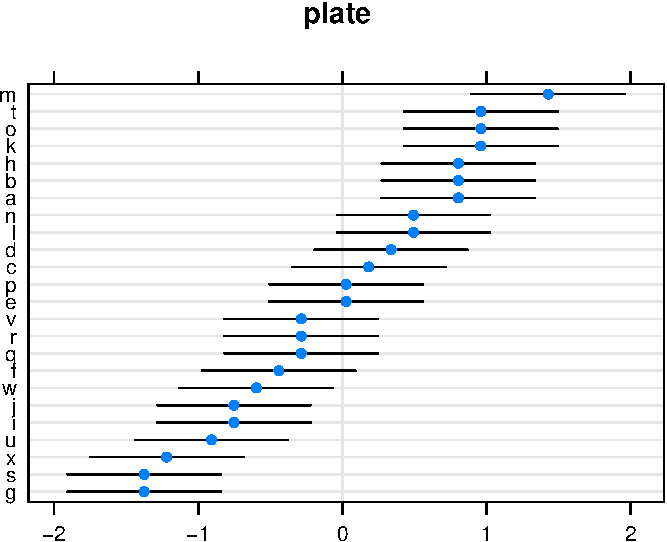
\includegraphics[width=0.5\linewidth]{Rcourse_files/figure-latex/unnamed-chunk-157-1}

The model seems to fit the data nicely.
A common measure of the goodness of fit is the \emph{coefficient of determination}, more commonly known as the \(R^2\).



\BeginKnitrBlock{definition}[R2]
\protect\hypertarget{def:unnamed-chunk-158}{}{\label{def:unnamed-chunk-158} \iffalse (R2) \fi{} }The coefficient of determination, denoted \(R^2\), is defined as
\begin{align}
  R^2:= 1-\frac{\sum_i (y_i - \hat y_i)^2}{\sum_i (y_i - \bar y)^2},
\end{align}
where \(\hat y_i\) is the model's prediction, \(\hat y_i = x_i \hat \beta\).
\EndKnitrBlock{definition}

It can be easily computed

\begin{Shaded}
\begin{Highlighting}[]
\KeywordTok{library}\NormalTok{(magrittr)}
\NormalTok{R2 <-}\StringTok{ }\ControlFlowTok{function}\NormalTok{(y, y.hat)\{}
\NormalTok{  numerator <-}\StringTok{ }\NormalTok{(y}\OperatorTok{-}\NormalTok{y.hat)}\OperatorTok{^}\DecValTok{2} \OperatorTok\StringTok{ }\NormalTok{sum}
\NormalTok{  denominator <-}\StringTok{ }\NormalTok{(y}\OperatorTok{-}\KeywordTok{mean}\NormalTok{(y))}\OperatorTok{^}\DecValTok{2} \OperatorTok\StringTok{ }\NormalTok{sum}
  \DecValTok{1}\OperatorTok{-}\NormalTok{numerator}\OperatorTok{/}\NormalTok{denominator}
\NormalTok{\}}
\KeywordTok{R2}\NormalTok{(}\DataTypeTok{y=}\NormalTok{whiteside[Insul}\OperatorTok{==}\StringTok{'Before'}\NormalTok{,Gas], }\DataTypeTok{y.hat=}\KeywordTok{predict}\NormalTok{(lm}\FloatTok{.1}\NormalTok{))}
\end{Highlighting}
\end{Shaded}

\begin{verbatim}
## [1] 0.9438081
\end{verbatim}

This is a nice result implying that about \(94\%\) of the variability in gas consumption can be attributed to changes in the outside temperature.

Obviously, R does provide the means to compute something as basic as \(R^2\), but I will let you find it for yourselves.

\hypertarget{inference}{%
\section{Inference}\label{inference}}

To perform inference on \(\hat \beta\), in order to test hypotheses and construct confidence intervals, we need to quantify the uncertainly in the reported \(\hat \beta\).
This is exactly what Eq.\eqref{eq:ols-distribution} gives us.

Luckily, we don't need to manipulate multivariate distributions manually, and everything we need is already implemented.
The most important function is \texttt{summary} which gives us an overview of the model's fit.
We emphasize that fitting a model with \texttt{lm} is an assumption free algorithmic step.
Inference using \texttt{summary} is \textbf{not} assumption free, and requires the set of assumptions leading to Eq.\eqref{eq:ols-distribution}.

\begin{Shaded}
\begin{Highlighting}[]
\KeywordTok{summary}\NormalTok{(lm}\FloatTok{.1}\NormalTok{)}
\end{Highlighting}
\end{Shaded}

\begin{verbatim}
## 
## Call:
## lm(formula = Gas ~ Temp, data = whiteside[Insul == "Before"])
## 
## Residuals:
##      Min       1Q   Median       3Q      Max 
## -0.62020 -0.19947  0.06068  0.16770  0.59778 
## 
## Coefficients:
##             Estimate Std. Error t value Pr(>|t|)    
## (Intercept)  6.85383    0.11842   57.88   <2e-16 ***
## Temp        -0.39324    0.01959  -20.08   <2e-16 ***
## ---
## Signif. codes:  0 '***' 0.001 '**' 0.01 '*' 0.05 '.' 0.1 ' ' 1
## 
## Residual standard error: 0.2813 on 24 degrees of freedom
## Multiple R-squared:  0.9438, Adjusted R-squared:  0.9415 
## F-statistic: 403.1 on 1 and 24 DF,  p-value: < 2.2e-16
\end{verbatim}

Things to note:

\begin{itemize}
\tightlist
\item
  The estimated \(\hat \beta\) is reported in the `Coefficients' table, which has point estimates, standard errors, t-statistics, and the p-values of a two-sided hypothesis test for each coefficient \(H_{0,j}:\beta_j=0, j=1,\dots,p\).
\item
  The \(R^2\) is reported at the bottom. The ``Adjusted R-squared'' is a variation that compensates for the model's complexity.
\item
  The original call to \texttt{lm} is saved in the \texttt{Call} section.
\item
  Some summary statistics of the residuals (\(y_i-\hat y_i\)) in the \texttt{Residuals} section.
\item
  The ``residuals standard error''\footnote{Sometimes known as the Root Mean Squared Error (RMSE).} is \(\sqrt{(n-p)^{-1} \sum_i (y_i-\hat y_i)^2}\). The denominator of this expression is the \emph{degrees of freedom}, \(n-p\), which can be thought of as the hardness of the problem.
\end{itemize}

As the name suggests, \texttt{summary} is merely a summary. The full \texttt{summary(lm.1)} object is a monstrous object.
Its various elements can be queried using \texttt{str(sumary(lm.1))}.

Can we check the assumptions required for inference?
Some.
Let's start with the linearity assumption.
If we were wrong, and the data is not arranged about a linear line, the residuals will have some shape. We thus plot the residuals as a function of the predictor to diagnose shape.

\begin{Shaded}
\begin{Highlighting}[]
\CommentTok{# errors (epsilons) vs. temperature, should oscillate around zero.}
\KeywordTok{plot}\NormalTok{(}\KeywordTok{residuals}\NormalTok{(lm}\FloatTok{.1}\NormalTok{)}\OperatorTok{~}\NormalTok{whiteside[Insul}\OperatorTok{==}\StringTok{'Before'}\NormalTok{,Temp])}
\KeywordTok{abline}\NormalTok{(}\DecValTok{0}\NormalTok{,}\DecValTok{0}\NormalTok{, }\DataTypeTok{lty=}\DecValTok{2}\NormalTok{)}
\end{Highlighting}
\end{Shaded}

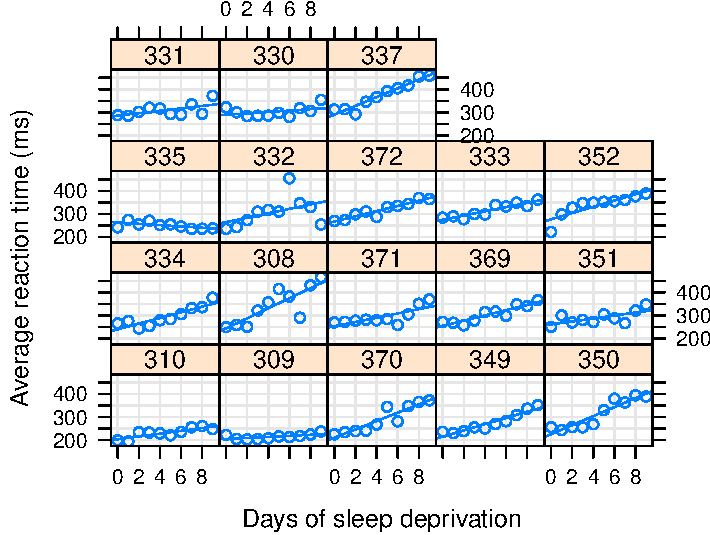
\includegraphics[width=0.5\linewidth]{Rcourse_files/figure-latex/unnamed-chunk-161-1}

I can't say I see any shape.
Let's fit a \textbf{wrong} model, just to see what ``shape'' means.

\begin{Shaded}
\begin{Highlighting}[]
\NormalTok{lm.}\FloatTok{1.1}\NormalTok{ <-}\StringTok{ }\KeywordTok{lm}\NormalTok{(Gas}\OperatorTok{~}\KeywordTok{I}\NormalTok{(Temp}\OperatorTok{^}\DecValTok{2}\NormalTok{), }\DataTypeTok{data=}\NormalTok{whiteside[Insul}\OperatorTok{==}\StringTok{'Before'}\NormalTok{,])}
\KeywordTok{plot}\NormalTok{(}\KeywordTok{residuals}\NormalTok{(lm.}\FloatTok{1.1}\NormalTok{)}\OperatorTok{~}\NormalTok{whiteside[Insul}\OperatorTok{==}\StringTok{'Before'}\NormalTok{,Temp]); }\KeywordTok{abline}\NormalTok{(}\DecValTok{0}\NormalTok{,}\DecValTok{0}\NormalTok{, }\DataTypeTok{lty=}\DecValTok{2}\NormalTok{)}
\end{Highlighting}
\end{Shaded}

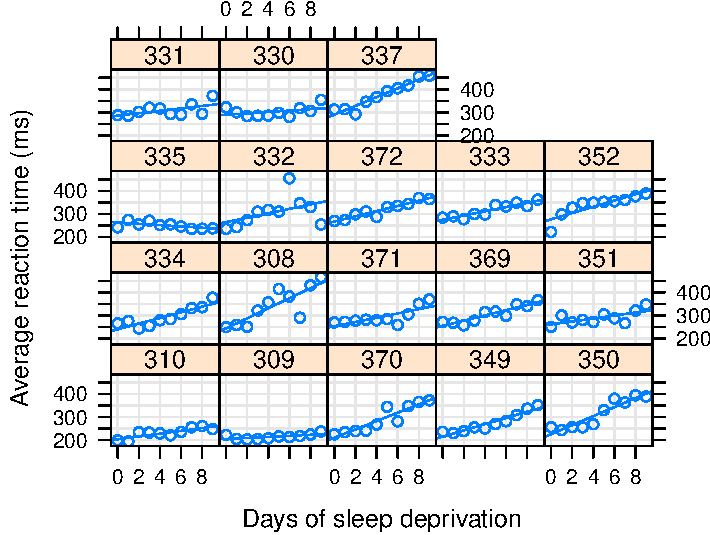
\includegraphics[width=0.5\linewidth]{Rcourse_files/figure-latex/unnamed-chunk-162-1}

Things to note:

\begin{itemize}
\tightlist
\item
  We used \texttt{I(Temp\^{}2)} to specify the model \(Gas=\beta_0 + \beta_1 Temp^2+ \varepsilon\).
\item
  The residuals have a ``belly''.
  Because they are not a cloud around the linear trend, and we have the wrong model.
\end{itemize}

To the next assumption.
We assumed \(\varepsilon_i\) are independent of everything else.
The residuals, \(y_i-\hat y_i\) can be thought of a sample of \(\varepsilon_i\).
When diagnosing the linearity assumption, we already saw their distribution does not vary with the \(x\)'s, \texttt{Temp} in our case.
They may be correlated with themselves; a positive departure from the model, may be followed by a series of positive departures etc.
Diagnosing these \emph{auto-correlations} is a real art, which is not part of our course.

The last assumption we required is normality.
As previously stated, if \(n \gg p\), this assumption can be relaxed.
If \(n\) is in the order of \(p\), we need to verify this assumption.
My favorite tool for this task is the \emph{qqplot}.
A qqplot compares the quantiles of the sample with the respective quantiles of the assumed distribution.
If quantiles align along a line, the assumed distribution is OK.
If quantiles depart from a line, then the assumed distribution does not fit the sample.

\begin{Shaded}
\begin{Highlighting}[]
\KeywordTok{qqnorm}\NormalTok{(}\KeywordTok{resid}\NormalTok{(lm}\FloatTok{.1}\NormalTok{))}
\end{Highlighting}
\end{Shaded}

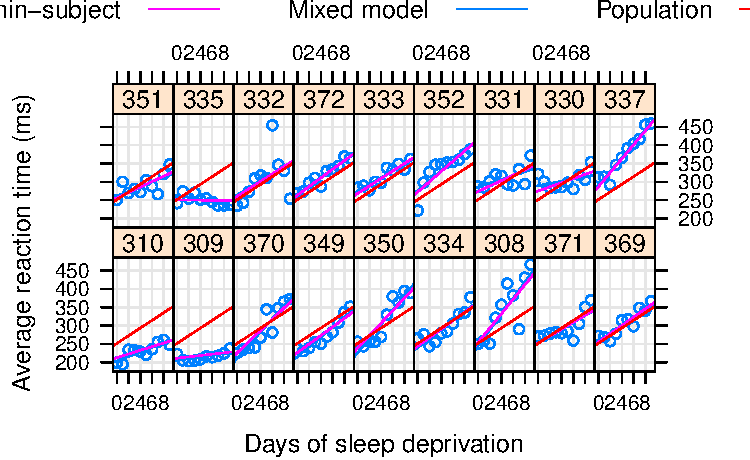
\includegraphics[width=0.5\linewidth]{Rcourse_files/figure-latex/unnamed-chunk-163-1}

Things to note:

\begin{itemize}
\tightlist
\item
  The \texttt{qqnorm} function plots a qqplot against a normal distribution. For non-normal distributions try \texttt{qqplot}.
\item
  \texttt{resid(lm.1)} extracts the residuals from the linear model, i.e., the vector of \(y_i-x_i'\hat \beta\).
\end{itemize}

Judging from the figure, the normality assumption is quite plausible.
Let's try the same on a non-normal sample, namely a uniformly distributed sample, to see how that would look.

\begin{Shaded}
\begin{Highlighting}[]
\KeywordTok{qqnorm}\NormalTok{(}\KeywordTok{runif}\NormalTok{(}\DecValTok{100}\NormalTok{))}
\end{Highlighting}
\end{Shaded}

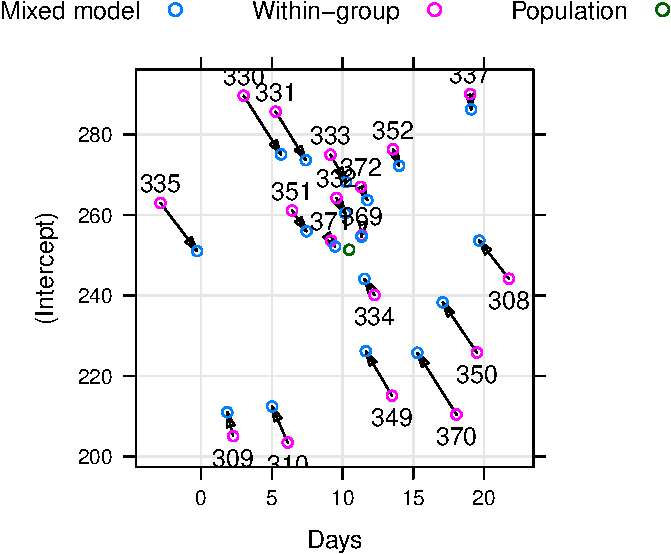
\includegraphics[width=0.5\linewidth]{Rcourse_files/figure-latex/unnamed-chunk-164-1}

\hypertarget{testing-a-hypothesis-on-a-single-coefficient}{%
\subsection{Testing a Hypothesis on a Single Coefficient}\label{testing-a-hypothesis-on-a-single-coefficient}}

The first inferential test we consider is a hypothesis test on a single coefficient.
In our gas example, we may want to test that the temperature has no effect on the gas consumption.
The answer for that is given immediately by \texttt{summary(lm.1)}

\begin{Shaded}
\begin{Highlighting}[]
\NormalTok{summary.lm1 <-}\StringTok{ }\KeywordTok{summary}\NormalTok{(lm}\FloatTok{.1}\NormalTok{)}
\NormalTok{coefs.lm1 <-}\StringTok{ }\NormalTok{summary.lm1}\OperatorTok{$}\NormalTok{coefficients}
\NormalTok{coefs.lm1}
\end{Highlighting}
\end{Shaded}

\begin{verbatim}
##               Estimate Std. Error   t value     Pr(>|t|)
## (Intercept)  6.8538277 0.11842341  57.87561 2.717533e-27
## Temp        -0.3932388 0.01958601 -20.07754 1.640469e-16
\end{verbatim}

We see that the p-value for \(H_{0,1}: \beta_1=0\) against a two sided alternative is effectively 0 (row 2 column 4), so that \(\beta_1\) is unlikely to be \(0\) (the null hypothesis can be rejected).

\hypertarget{constructing-a-confidence-interval-on-a-single-coefficient}{%
\subsection{Constructing a Confidence Interval on a Single Coefficient}\label{constructing-a-confidence-interval-on-a-single-coefficient}}

Since the \texttt{summary} function gives us the standard errors of \(\hat \beta\), we can immediately compute \(\hat \beta_j \pm 2 \sqrt{Var[\hat \beta_j]}\) to get ourselves a (roughly) \(95\%\) confidence interval.
In our example the interval is

\begin{Shaded}
\begin{Highlighting}[]
\NormalTok{coefs.lm1[}\DecValTok{2}\NormalTok{,}\DecValTok{1}\NormalTok{] }\OperatorTok{+}\StringTok{ }\KeywordTok{c}\NormalTok{(}\OperatorTok{-}\DecValTok{2}\NormalTok{,}\DecValTok{2}\NormalTok{) }\OperatorTok{*}\StringTok{ }\NormalTok{coefs.lm1[}\DecValTok{2}\NormalTok{,}\DecValTok{2}\NormalTok{]}
\end{Highlighting}
\end{Shaded}

\begin{verbatim}
## [1] -0.4324108 -0.3540668
\end{verbatim}

Things to note:

\begin{itemize}
\tightlist
\item
  The function \texttt{confint(lm.1)} can calculate it. Sometimes it's more simple to write 20 characters of code than finding a function that does it for us.
\end{itemize}

\hypertarget{multiple-regression}{%
\subsection{Multiple Regression}\label{multiple-regression}}

\BeginKnitrBlock{remark}
\iffalse{} {Remark. } \fi{}\emph{Multiple regression} is not to be confused with \emph{multivariate regression} discussed in Chapter \ref{multivariate}.
\EndKnitrBlock{remark}

The \texttt{swiss} dataset encodes the fertility at each of Switzerland's 47 French speaking provinces, along other socio-economic indicators. Let's see if these are statistically related:

\begin{Shaded}
\begin{Highlighting}[]
\KeywordTok{head}\NormalTok{(swiss)}
\end{Highlighting}
\end{Shaded}

\begin{verbatim}
##              Fertility Agriculture Examination Education Catholic
## Courtelary        80.2        17.0          15        12     9.96
## Delemont          83.1        45.1           6         9    84.84
## Franches-Mnt      92.5        39.7           5         5    93.40
## Moutier           85.8        36.5          12         7    33.77
## Neuveville        76.9        43.5          17        15     5.16
## Porrentruy        76.1        35.3           9         7    90.57
##              Infant.Mortality
## Courtelary               22.2
## Delemont                 22.2
## Franches-Mnt             20.2
## Moutier                  20.3
## Neuveville               20.6
## Porrentruy               26.6
\end{verbatim}

\begin{Shaded}
\begin{Highlighting}[]
\NormalTok{lm}\FloatTok{.5}\NormalTok{ <-}\StringTok{ }\KeywordTok{lm}\NormalTok{(}\DataTypeTok{data=}\NormalTok{swiss, Fertility}\OperatorTok{~}\NormalTok{Agriculture}\OperatorTok{+}\NormalTok{Examination}\OperatorTok{+}\NormalTok{Education}\OperatorTok{+}\NormalTok{Catholic}\OperatorTok{+}\NormalTok{Infant.Mortality)}
\KeywordTok{summary}\NormalTok{(lm}\FloatTok{.5}\NormalTok{)}
\end{Highlighting}
\end{Shaded}

\begin{verbatim}
## 
## Call:
## lm(formula = Fertility ~ Agriculture + Examination + Education + 
##     Catholic + Infant.Mortality, data = swiss)
## 
## Residuals:
##      Min       1Q   Median       3Q      Max 
## -15.2743  -5.2617   0.5032   4.1198  15.3213 
## 
## Coefficients:
##                  Estimate Std. Error t value Pr(>|t|)    
## (Intercept)      66.91518   10.70604   6.250 1.91e-07 ***
## Agriculture      -0.17211    0.07030  -2.448  0.01873 *  
## Examination      -0.25801    0.25388  -1.016  0.31546    
## Education        -0.87094    0.18303  -4.758 2.43e-05 ***
## Catholic          0.10412    0.03526   2.953  0.00519 ** 
## Infant.Mortality  1.07705    0.38172   2.822  0.00734 ** 
## ---
## Signif. codes:  0 '***' 0.001 '**' 0.01 '*' 0.05 '.' 0.1 ' ' 1
## 
## Residual standard error: 7.165 on 41 degrees of freedom
## Multiple R-squared:  0.7067, Adjusted R-squared:  0.671 
## F-statistic: 19.76 on 5 and 41 DF,  p-value: 5.594e-10
\end{verbatim}

Things to note:

\begin{itemize}
\tightlist
\item
  The \texttt{\textasciitilde{}} syntax allows to specify various predictors separated by the \texttt{+} operator.
\item
  The summary of the model now reports the estimated effect, i.e., the regression coefficient, of each of the variables.
\end{itemize}

Clearly, naming each variable explicitly is a tedious task if there are many. The use of \texttt{Fertility\textasciitilde{}.} in the next example reads: ``Fertility as a function of all other variables in the \texttt{swiss} data.frame''.

\begin{Shaded}
\begin{Highlighting}[]
\NormalTok{lm}\FloatTok{.5}\NormalTok{ <-}\StringTok{ }\KeywordTok{lm}\NormalTok{(}\DataTypeTok{data=}\NormalTok{swiss, Fertility}\OperatorTok{~}\NormalTok{.)}
\KeywordTok{summary}\NormalTok{(lm}\FloatTok{.5}\NormalTok{)}
\end{Highlighting}
\end{Shaded}

\begin{verbatim}
## 
## Call:
## lm(formula = Fertility ~ ., data = swiss)
## 
## Residuals:
##      Min       1Q   Median       3Q      Max 
## -15.2743  -5.2617   0.5032   4.1198  15.3213 
## 
## Coefficients:
##                  Estimate Std. Error t value Pr(>|t|)    
## (Intercept)      66.91518   10.70604   6.250 1.91e-07 ***
## Agriculture      -0.17211    0.07030  -2.448  0.01873 *  
## Examination      -0.25801    0.25388  -1.016  0.31546    
## Education        -0.87094    0.18303  -4.758 2.43e-05 ***
## Catholic          0.10412    0.03526   2.953  0.00519 ** 
## Infant.Mortality  1.07705    0.38172   2.822  0.00734 ** 
## ---
## Signif. codes:  0 '***' 0.001 '**' 0.01 '*' 0.05 '.' 0.1 ' ' 1
## 
## Residual standard error: 7.165 on 41 degrees of freedom
## Multiple R-squared:  0.7067, Adjusted R-squared:  0.671 
## F-statistic: 19.76 on 5 and 41 DF,  p-value: 5.594e-10
\end{verbatim}

\hypertarget{anova}{%
\subsection{ANOVA (*)}\label{anova}}

Our next example\footnote{The example is taken from \url{http://rtutorialseries.blogspot.co.il/2011/02/r-tutorial-series-two-way-anova-with.html}} contains a hypothetical sample of \(60\) participants who are divided into three stress reduction treatment groups (mental, physical, and medical) and three age groups groups.
The stress reduction values are represented on a scale that ranges from 1 to 10.
The values represent how effective the treatment programs were at reducing participant's stress levels, with larger effects indicating higher effectiveness.

\begin{Shaded}
\begin{Highlighting}[]
\NormalTok{twoWay <-}\StringTok{ }\KeywordTok{read.csv}\NormalTok{(}\StringTok{'data/dataset_anova_twoWay_comparisons.csv'}\NormalTok{)}
\KeywordTok{head}\NormalTok{(twoWay)}
\end{Highlighting}
\end{Shaded}

\begin{verbatim}
##   Treatment   Age StressReduction
## 1    mental young              10
## 2    mental young               9
## 3    mental young               8
## 4    mental   mid               7
## 5    mental   mid               6
## 6    mental   mid               5
\end{verbatim}

How many observations per group?

\begin{Shaded}
\begin{Highlighting}[]
\KeywordTok{table}\NormalTok{(twoWay}\OperatorTok{$}\NormalTok{Treatment, twoWay}\OperatorTok{$}\NormalTok{Age)}
\end{Highlighting}
\end{Shaded}

\begin{verbatim}
##           
##            mid old young
##   medical    3   3     3
##   mental     3   3     3
##   physical   3   3     3
\end{verbatim}

Since we have two factorial predictors, this multiple regression is nothing but a \emph{two way ANOVA}.
Let's fit the model and inspect it.

\begin{Shaded}
\begin{Highlighting}[]
\NormalTok{lm}\FloatTok{.2}\NormalTok{ <-}\StringTok{ }\KeywordTok{lm}\NormalTok{(StressReduction}\OperatorTok{~}\NormalTok{.,}\DataTypeTok{data=}\NormalTok{twoWay)}
\KeywordTok{summary}\NormalTok{(lm}\FloatTok{.2}\NormalTok{)}
\end{Highlighting}
\end{Shaded}

\begin{verbatim}
## 
## Call:
## lm(formula = StressReduction ~ ., data = twoWay)
## 
## Residuals:
##    Min     1Q Median     3Q    Max 
##     -1     -1      0      1      1 
## 
## Coefficients:
##                   Estimate Std. Error t value Pr(>|t|)    
## (Intercept)         4.0000     0.3892  10.276 7.34e-10 ***
## Treatmentmental     2.0000     0.4264   4.690 0.000112 ***
## Treatmentphysical   1.0000     0.4264   2.345 0.028444 *  
## Ageold             -3.0000     0.4264  -7.036 4.65e-07 ***
## Ageyoung            3.0000     0.4264   7.036 4.65e-07 ***
## ---
## Signif. codes:  0 '***' 0.001 '**' 0.01 '*' 0.05 '.' 0.1 ' ' 1
## 
## Residual standard error: 0.9045 on 22 degrees of freedom
## Multiple R-squared:  0.9091, Adjusted R-squared:  0.8926 
## F-statistic:    55 on 4 and 22 DF,  p-value: 3.855e-11
\end{verbatim}

Things to note:

\begin{itemize}
\item
  The \texttt{StressReduction\textasciitilde{}.} syntax is read as ``Stress reduction as a function of everything else''.
\item
  All the (main) effects and the intercept seem to be significant.
\item
  Mid age and medical treatment are missing, hence it is implied that they are the baseline, and this model accounts for the departure from this baseline.
\item
  The data has 2 factors, but the coefficients table has 4 predictors. This is because \texttt{lm} noticed that \texttt{Treatment} and \texttt{Age} are factors. Each level of each factor is thus encoded as a different (dummy) variable.
  The numerical values of the factors are meaningless.
  Instead, R has constructed a dummy variable for each level of each factor.
  The names of the effect are a concatenation of the factor's name, and its level.
  You can inspect these dummy variables with the \texttt{model.matrix} command.
\end{itemize}

\begin{Shaded}
\begin{Highlighting}[]
\KeywordTok{model.matrix}\NormalTok{(lm}\FloatTok{.2}\NormalTok{) }\OperatorTok\StringTok{ }\NormalTok{lattice}\OperatorTok{::}\KeywordTok{levelplot}\NormalTok{()}
\end{Highlighting}
\end{Shaded}

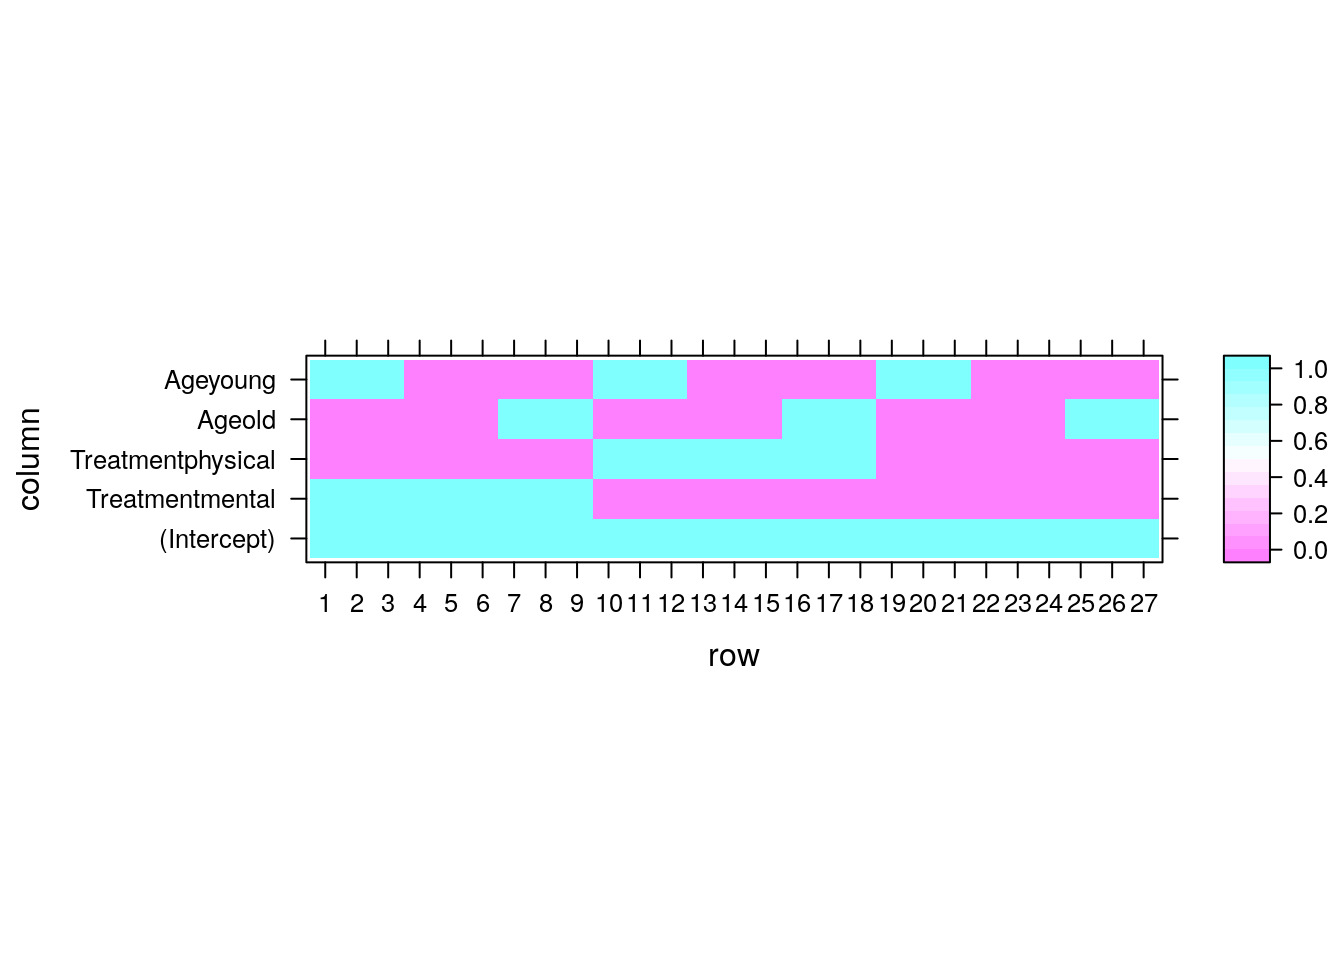
\includegraphics[width=0.5\linewidth]{Rcourse_files/figure-latex/unnamed-chunk-173-1}
If you don't want the default dummy coding, look at \texttt{?contrasts}.

If you are more familiar with the ANOVA literature, or that you don't want the effects of each level separately, but rather, the effect of \textbf{all} the levels of each factor, use the \texttt{anova} command.

\begin{Shaded}
\begin{Highlighting}[]
\KeywordTok{anova}\NormalTok{(lm}\FloatTok{.2}\NormalTok{)}
\end{Highlighting}
\end{Shaded}

\begin{verbatim}
## Analysis of Variance Table
## 
## Response: StressReduction
##           Df Sum Sq Mean Sq F value    Pr(>F)    
## Treatment  2     18   9.000      11 0.0004883 ***
## Age        2    162  81.000      99     1e-11 ***
## Residuals 22     18   0.818                      
## ---
## Signif. codes:  0 '***' 0.001 '**' 0.01 '*' 0.05 '.' 0.1 ' ' 1
\end{verbatim}

Things to note:

\begin{itemize}
\tightlist
\item
  The ANOVA table, unlike the \texttt{summary} function, tests if \textbf{any} of the levels of a factor has an effect, and not one level at a time.
\item
  The significance of each factor is computed using an F-test.
\item
  The degrees of freedom, encoding the number of levels of a factor, is given in the \texttt{Df} column.
\item
  The StressReduction seems to vary for different ages and treatments, since both factors are significant.
\end{itemize}

If you are extremely more comfortable with the ANOVA literature, you could have replaced the \texttt{lm} command with the \texttt{aov} command all along.

\begin{Shaded}
\begin{Highlighting}[]
\NormalTok{lm.}\FloatTok{2.2}\NormalTok{ <-}\StringTok{ }\KeywordTok{aov}\NormalTok{(StressReduction}\OperatorTok{~}\NormalTok{.,}\DataTypeTok{data=}\NormalTok{twoWay)}
\KeywordTok{class}\NormalTok{(lm.}\FloatTok{2.2}\NormalTok{)}
\end{Highlighting}
\end{Shaded}

\begin{verbatim}
## [1] "aov" "lm"
\end{verbatim}

\begin{Shaded}
\begin{Highlighting}[]
\KeywordTok{summary}\NormalTok{(lm.}\FloatTok{2.2}\NormalTok{)}
\end{Highlighting}
\end{Shaded}

\begin{verbatim}
##             Df Sum Sq Mean Sq F value   Pr(>F)    
## Treatment    2     18    9.00      11 0.000488 ***
## Age          2    162   81.00      99    1e-11 ***
## Residuals   22     18    0.82                     
## ---
## Signif. codes:  0 '***' 0.001 '**' 0.01 '*' 0.05 '.' 0.1 ' ' 1
\end{verbatim}

Things to note:

\begin{itemize}
\tightlist
\item
  The \texttt{lm} function has been replaced with an \texttt{aov} function.
\item
  The output of \texttt{aov} is an \texttt{aov} class object, which extends the \texttt{lm} class.
\item
  The summary of an \texttt{aov} is not like the summary of an \texttt{lm} object, but rather, like an ANOVA table.
\end{itemize}

As in any two-way ANOVA, we may want to ask if different age groups respond differently to different treatments.
In the statistical parlance, this is called an \emph{interaction}, or more precisely, an \emph{interaction of order 2}.

\begin{Shaded}
\begin{Highlighting}[]
\NormalTok{lm}\FloatTok{.3}\NormalTok{ <-}\StringTok{ }\KeywordTok{lm}\NormalTok{(StressReduction}\OperatorTok{~}\NormalTok{Treatment}\OperatorTok{+}\NormalTok{Age}\OperatorTok{+}\NormalTok{Treatment}\OperatorTok{:}\NormalTok{Age}\DecValTok{-1}\NormalTok{,}\DataTypeTok{data=}\NormalTok{twoWay)}
\end{Highlighting}
\end{Shaded}

The syntax \texttt{StressReduction\textasciitilde{}Treatment+Age+Treatment:Age-1} tells R to include main effects of Treatment, Age, and their interactions. The -1 removes the intercept.
Here are other ways to specify the same model.

\begin{Shaded}
\begin{Highlighting}[]
\NormalTok{lm}\FloatTok{.3}\NormalTok{ <-}\StringTok{ }\KeywordTok{lm}\NormalTok{(StressReduction }\OperatorTok{~}\StringTok{ }\NormalTok{Treatment }\OperatorTok{*}\StringTok{ }\NormalTok{Age }\OperatorTok{-}\StringTok{ }\DecValTok{1}\NormalTok{,}\DataTypeTok{data=}\NormalTok{twoWay)}
\NormalTok{lm}\FloatTok{.3}\NormalTok{ <-}\StringTok{ }\KeywordTok{lm}\NormalTok{(StressReduction}\OperatorTok{~}\NormalTok{(.)}\OperatorTok{^}\DecValTok{2} \OperatorTok{-}\StringTok{ }\DecValTok{1}\NormalTok{,}\DataTypeTok{data=}\NormalTok{twoWay)}
\end{Highlighting}
\end{Shaded}

The syntax \texttt{Treatment\ *\ Age} means ``main effects with second order interactions''.
The syntax \texttt{(.)\^{}2} means ``everything with second order interactions'', this time we don't have I() as in the temperature example because here we want the second order interaction and not the square of each variable.

Let's inspect the model

\begin{Shaded}
\begin{Highlighting}[]
\KeywordTok{summary}\NormalTok{(lm}\FloatTok{.3}\NormalTok{)}
\end{Highlighting}
\end{Shaded}

\begin{verbatim}
## 
## Call:
## lm(formula = StressReduction ~ Treatment + Age + Treatment:Age - 
##     1, data = twoWay)
## 
## Residuals:
##    Min     1Q Median     3Q    Max 
##     -1     -1      0      1      1 
## 
## Coefficients:
##                              Estimate Std. Error t value Pr(>|t|)    
## Treatmentmedical            4.000e+00  5.774e-01   6.928 1.78e-06 ***
## Treatmentmental             6.000e+00  5.774e-01  10.392 4.92e-09 ***
## Treatmentphysical           5.000e+00  5.774e-01   8.660 7.78e-08 ***
## Ageold                     -3.000e+00  8.165e-01  -3.674  0.00174 ** 
## Ageyoung                    3.000e+00  8.165e-01   3.674  0.00174 ** 
## Treatmentmental:Ageold      4.246e-16  1.155e+00   0.000  1.00000    
## Treatmentphysical:Ageold    1.034e-15  1.155e+00   0.000  1.00000    
## Treatmentmental:Ageyoung   -3.126e-16  1.155e+00   0.000  1.00000    
## Treatmentphysical:Ageyoung  5.128e-16  1.155e+00   0.000  1.00000    
## ---
## Signif. codes:  0 '***' 0.001 '**' 0.01 '*' 0.05 '.' 0.1 ' ' 1
## 
## Residual standard error: 1 on 18 degrees of freedom
## Multiple R-squared:  0.9794, Adjusted R-squared:  0.9691 
## F-statistic:    95 on 9 and 18 DF,  p-value: 2.556e-13
\end{verbatim}

Things to note:

\begin{itemize}
\tightlist
\item
  There are still \(5\) main effects, but also \(4\) interactions.
  This is because when allowing a different average response for every \(Treatment*Age\) combination, we are effectively estimating \(3*3=9\) cell means, even if they are not parametrized as cell means, but rather as main effect and interactions.
\item
  The interactions do not seem to be significant.
\item
  The assumptions required for inference are clearly not met in this example, which is there just to demonstrate R's capabilities.
\end{itemize}

Asking if all the interactions are significant, is asking if the different age groups have the same response to different treatments.
Can we answer that based on the various interactions?
We might, but it is possible that no single interaction is significant, while the combination is.
To test for all the interactions together, we can simply check if the model without interactions is (significantly) better than a model with interactions. I.e., compare \texttt{lm.2} to \texttt{lm.3}.
This is done with the \texttt{anova} command.

\begin{Shaded}
\begin{Highlighting}[]
\KeywordTok{anova}\NormalTok{(lm}\FloatTok{.2}\NormalTok{,lm}\FloatTok{.3}\NormalTok{, }\DataTypeTok{test=}\StringTok{'F'}\NormalTok{)}
\end{Highlighting}
\end{Shaded}

\begin{verbatim}
## Analysis of Variance Table
## 
## Model 1: StressReduction ~ Treatment + Age
## Model 2: StressReduction ~ Treatment + Age + Treatment:Age - 1
##   Res.Df RSS Df   Sum of Sq F Pr(>F)
## 1     22  18                        
## 2     18  18  4 -3.5527e-15
\end{verbatim}

We see that \texttt{lm.3} is \textbf{not} (significantly) better than \texttt{lm.2}, so that we can conclude that there are no interactions: different ages have the same response to different treatments.

\hypertarget{testing-a-hypothesis-on-a-single-contrast}{%
\subsection{Testing a Hypothesis on a Single Contrast (*)}\label{testing-a-hypothesis-on-a-single-contrast}}

Returning to the model without interactions, \texttt{lm.2}.

\begin{Shaded}
\begin{Highlighting}[]
\KeywordTok{coef}\NormalTok{(}\KeywordTok{summary}\NormalTok{(lm}\FloatTok{.2}\NormalTok{))}
\end{Highlighting}
\end{Shaded}

\begin{verbatim}
##                   Estimate Std. Error   t value     Pr(>|t|)
## (Intercept)              4  0.3892495 10.276186 7.336391e-10
## Treatmentmental          2  0.4264014  4.690416 1.117774e-04
## Treatmentphysical        1  0.4264014  2.345208 2.844400e-02
## Ageold                  -3  0.4264014 -7.035624 4.647299e-07
## Ageyoung                 3  0.4264014  7.035624 4.647299e-07
\end{verbatim}

We see that the effect of the various treatments is rather similar.
It is possible that all treatments actually have the same effect.
Comparing the effects of factor levels is called a \emph{contrast}.
Let's test if the medical treatment, has in fact, the same effect as the physical treatment.

\begin{Shaded}
\begin{Highlighting}[]
\KeywordTok{library}\NormalTok{(multcomp)}
\NormalTok{my.contrast <-}\StringTok{ }\KeywordTok{matrix}\NormalTok{(}\KeywordTok{c}\NormalTok{(}\OperatorTok{-}\DecValTok{1}\NormalTok{,}\DecValTok{0}\NormalTok{,}\DecValTok{1}\NormalTok{,}\DecValTok{0}\NormalTok{,}\DecValTok{0}\NormalTok{), }\DataTypeTok{nrow =}  \DecValTok{1}\NormalTok{)}
\NormalTok{lm}\FloatTok{.4}\NormalTok{ <-}\StringTok{ }\KeywordTok{glht}\NormalTok{(lm}\FloatTok{.2}\NormalTok{, }\DataTypeTok{linfct=}\NormalTok{my.contrast)}
\KeywordTok{summary}\NormalTok{(lm}\FloatTok{.4}\NormalTok{)}
\end{Highlighting}
\end{Shaded}

\begin{verbatim}
## 
##   Simultaneous Tests for General Linear Hypotheses
## 
## Fit: lm(formula = StressReduction ~ ., data = twoWay)
## 
## Linear Hypotheses:
##        Estimate Std. Error t value Pr(>|t|)    
## 1 == 0  -3.0000     0.7177   -4.18 0.000389 ***
## ---
## Signif. codes:  0 '***' 0.001 '**' 0.01 '*' 0.05 '.' 0.1 ' ' 1
## (Adjusted p values reported -- single-step method)
\end{verbatim}

Things to note:

\begin{itemize}
\tightlist
\item
  A contrast is a linear function of the coefficients. In our example \(H_0:\beta_1-\beta_3=0\), which justifies the construction of \texttt{my.contrast}.
\item
  We used the \texttt{glht} function (generalized linear hypothesis test) from the package \textbf{multcomp}.
\item
  The contrast is significant, i.e., the effect of a medical treatment, is different than that of a physical treatment.
\end{itemize}

\hypertarget{extra-diagnostics}{%
\section{Extra Diagnostics}\label{extra-diagnostics}}

\hypertarget{diagnosing-heteroskedasticity}{%
\subsection{Diagnosing Heteroskedasticity}\label{diagnosing-heteroskedasticity}}

Textbook assumptions for inference on \(\hat \beta_{OLS}\) include the \emph{homoskedasticiy} assumption, i.e., \(Var[\varepsilon]\) is fixed and independent of everyhting.
This comes from viewing \(\varepsilon\) as a measurement error.
It may not be the case when viewing \(\varepsilon\) as ``all other effect not included in the model''.
In technical terms, homoskedastocity implies that \(Var[\varepsilon]\) is a scaled identity matrix.
Heteroskedasticity means that \(Var[\varepsilon]\) is a diagonal matrix.
Because a scaled identify matrix implies that the quantiles of a multivariate Gaussian are spheres, testing for heteroskedasticity is also known as a \emph{Sphericity Test}.

Can we verify homoskedasticity, and do we need it?

To verify homoskedasticity we only need to look at the residuals of a model. If they seem to have the same variability for all \(x\) we are clear.
If \(x\) is multivariate, and we cannot visualise residuals, \(y_i-\hat y_i\) as a function of \(x\), then visualising it as a function of \(\hat y_i\) is also good.

Another way of dealing with heteroskedasticity is by estimating variances for groups of observations separately.
This is the \emph{Cluster Robust Standard Errors} discussed in \ref{cr-se}.

Can use perform a test to infer homoskedasticity?
In the frequentist hypotesis testing framework we can only reject homoskedasticity, not accept it.
In the \href{https://en.wikipedia.org/wiki/Bayesian_inference}{Bayesian hypotesis testing} framework we can indeed infer homoskedasticity, but one would have to defend his/her priors.

For some tests that detect heteroskedasticity see the \href{https://cran.r-project.org/web/packages/olsrr/vignettes/heteroskedasticity.html}{olsrr} package.
For an econometric flavored approach to the problem, see the \href{https://cran.r-project.org/package=plm}{plm} package, and its excellent \href{https://cran.r-project.org/web/packages/plm/vignettes/plmPackage.html}{vignette}.

\hypertarget{diagnosing-multicolinearity}{%
\subsection{Diagnosing Multicolinearity}\label{diagnosing-multicolinearity}}

When designing an experiment (e.g. \href{https://en.wikipedia.org/wiki/Randomized_controlled_trial}{RCTs}) we will assure treatments are ``balanced'', so that one effect estimates are not correlated.
This is not always possible, especially not in observational studies.
If various variables capture the same effect, the certainty in the effect will ``spread'' over these variables.
Formally: the standard errros of effect estimates will increase.
Perhaps more importantly- causal inference with correlated predictors is very hard to interpret, because changes in outcome may be attibuted to any on of the (correlated) predictors.

We will eschew the complicated philosophical implication of causal infernece with correlated predictors, and merely refer the reader to the package \href{https://cran.r-project.org/web/packages/olsrr/vignettes/regression_diagnostics.html}{olsrr} for some popular tools to diagnose multicolinearity.

\hypertarget{bibliographic-notes-4}{%
\section{Bibliographic Notes}\label{bibliographic-notes-4}}

Like any other topic in this book, you can consult \citet{venables2013modern} for more on linear models.
For the theory of linear models, I like \citet{greene2003econometric}.

\hypertarget{practice-yourself-3}{%
\section{Practice Yourself}\label{practice-yourself-3}}

\begin{enumerate}
\def\labelenumi{\arabic{enumi}.}
\item
  Inspect women's heights and weights with \texttt{?women}.

  \begin{enumerate}
  \def\labelenumii{\arabic{enumii}.}
  \tightlist
  \item
    What is the change in weight per unit change in height? Use the \texttt{lm} function.
  \item
    Is the relation of height on weight significant? Use \texttt{summary}.
  \item
    Plot the residuals of the linear model with \texttt{plot} and \texttt{resid}.
  \item
    Plot the predictions of the model using \texttt{abline}.
  \item
    Inspect the normality of residuals using \texttt{qqnorm}.
  \item
    Inspect the design matrix using \texttt{model.matrix}.
  \end{enumerate}
\item
  Write a function that takes an \texttt{lm} class object, and returns the confidence interval on the first coefficient. Apply it on the height and weight data.
\item
  Use the \texttt{ANOVA} function to test the significance of the effect of height.
\item
  Read about the ``mtcars'' dataset using \texttt{?\ mtcars}. Inspect the dependency of the fuel consumption (mpg) in the weight (wt) and the 1/4 mile time (qsec).

  \begin{enumerate}
  \def\labelenumii{\arabic{enumii}.}
  \tightlist
  \item
    Make a pairs scatter plot with \texttt{plot(mtcars{[},c("mpg","wt","qsec"){]})}
    Does the connection look linear?
  \item
    Fit a multiple linear regression with \texttt{lm}. Call it \texttt{model1}.
  \item
    Try to add the transmission (am) as independent variable. Let R know this is a categorical variable with \texttt{factor(am)}. Call it \texttt{model2}.
  \item
    Compare the ``Adjusted R-squared'' measure of the two models (we can't use the regular R2 to compare two models with a different number of variables).
  \item
    Do the coefficients significant?
  \item
    Inspect the normality of residuals and the linearity assumptions.
  \item
    Now Inspect the hypothesis that the effect of weight is different between the transmission types with adding interaction to the model \texttt{wt*factor(am)}.
  \item
    According to this model, what is the addition of one unit of weight in a manual transmission to the fuel consumption (-2.973-4.141=-7.11)?
  \end{enumerate}
\end{enumerate}

\hypertarget{glm}{%
\chapter{Generalized Linear Models}\label{glm}}

\BeginKnitrBlock{example}
\protect\hypertarget{exm:cigarettes}{}{\label{exm:cigarettes} }Consider the relation between cigarettes smoked, and the occurance of lung cancer.
Do we expect the probability of cancer to be linear in the number of cigarettes? Probably not.
Do we expect the variability of events to be constant about the trend? Probably not.
\EndKnitrBlock{example}

\BeginKnitrBlock{example}
\protect\hypertarget{exm:cars}{}{\label{exm:cars} }Consider the relation between the travel times to the distance travelled.
Do you agree that the longer the distance travelled, then not only the travel times get longer, but they also get more variable?
\EndKnitrBlock{example}

\hypertarget{problem-setup-1}{%
\section{Problem Setup}\label{problem-setup-1}}

In the Linear Models Chapter \ref{lm}, we assumed the generative process to be linear in the effects of the predictors \(x\).
We now write that same linear model, slightly differently:
\[
 y|x \sim \mathcal{N}(x'\beta, \sigma^2).
\]

This model not allow for the non-linear relations of Example \ref{exm:cigarettes}, nor does it allow for the distribution of \(\varepsilon\) to change with \(x\), as in Example \ref{exm:cars}.
\emph{Generalize linear models} (GLM), as the name suggests, are a generalization of the linear models in Chapter \ref{lm} that allow that\footnote{Do not confuse \emph{generalized linear models} with \href{https://en.wikipedia.org/wiki/Nonlinear_regression}{\emph{non-linear regression}}, or \href{https://en.wikipedia.org/wiki/Generalized_least_squares}{\emph{generalized least squares}}.
  These are different things, that we do not discuss.}.

For Example \ref{exm:cigarettes}, we would like something in the lines of
\[
 y|x \sim Binom(1,p(x))
\]

For Example \ref{exm:cars}, we would like something in the lines of
\[
 y|x \sim \mathcal{N}(x'\beta,\sigma^2(x)),
\]
or more generally
\[
 y|x \sim \mathcal{N}(\mu(x),\sigma^2(x)),
\]
or maybe not Gaussian
\[
 y|x \sim Pois(\lambda(x)).
\]

Even more generally, for some distribution \(F(\theta)\), with a parameter \(\theta\), we would like to assume that the data is generated via
\begin{align}
  \label{eq:general}
  y|x \sim F(\theta(x))
\end{align}

Possible examples include
\begin{align}
 y|x &\sim Poisson(\lambda(x)) \\
 y|x &\sim Exp(\lambda(x)) \\
 y|x &\sim \mathcal{N}(\mu(x),\sigma^2(x)) 
\end{align}

GLMs allow models of the type of Eq.\eqref{eq:general}, while imposing some constraints on \(F\) and on the relation \(\theta(x)\).
GLMs assume the data distribution \(F\) to be in a ``well-behaved'' family known as the \href{https://en.wikipedia.org/wiki/Natural_exponential_family}{\emph{Natural Exponential Family}} of distributions.
This family includes the Gaussian, Gamma, Binomial, Poisson, and Negative Binomial distributions.
These five include as special cases the exponential, chi-squared, Rayleigh, Weibull, Bernoulli, and geometric distributions.

GLMs also assume that the distribution's parameter, \(\theta\), is some simple function of a linear combination of the effects.
In our cigarettes example this amounts to assuming that each cigarette has an additive effect, but not on the probability of cancer, but rather, on some simple function of it.
Formally
\[g(\theta(x))=x'\beta,\] and we recall that \[x'\beta=\beta_0 + \sum_j x_j \beta_j.\]
The function \(g\) is called the \emph{link} function, its inverse, \(g^{-1}\) is the \emph{mean function}.
We thus say that ``the effects of each cigarette is linear \textbf{in link scale}''.
This terminology will later be required to understand R's output.

\hypertarget{logistic-regression}{%
\section{Logistic Regression}\label{logistic-regression}}

The best known of the GLM class of models is the \emph{logistic regression} that deals with Binomial, or more precisely, Bernoulli-distributed data.
The link function in the logistic regression is the \emph{logit function}
\begin{align}
  g(t)=log\left( \frac{t}{(1-t)} \right)
  \label{eq:logistic-link}  
\end{align}
implying that under the logistic model assumptions
\begin{align}
  y|x \sim Binom \left( 1, p=\frac{e^{x'\beta}}{1+e^{x'\beta}} \right).
  \label{eq:logistic}
\end{align}

Before we fit such a model, we try to justify this construction, in particular, the enigmatic link function in Eq.\eqref{eq:logistic-link}.
Let's look at the simplest possible case: the comparison of two groups indexed by \(x\): \(x=0\) for the first, and \(x=1\) for the second.
We start with some definitions.

\BeginKnitrBlock{definition}[Odds]
\protect\hypertarget{def:unnamed-chunk-182}{}{\label{def:unnamed-chunk-182} \iffalse (Odds) \fi{} }The \emph{odds}, of a binary random variable, \(y\), is defined as \[\frac{P(y=1)}{P(y=0)}.\]
\EndKnitrBlock{definition}

Odds are the same as probabilities, but instead of telling me there is a \(66\%\) of success, they tell me the odds of success are ``2 to 1''.
If you ever placed a bet, the language of ``odds'' should not be unfamiliar to you.

\BeginKnitrBlock{definition}[Odds Ratio]
\protect\hypertarget{def:unnamed-chunk-183}{}{\label{def:unnamed-chunk-183} \iffalse (Odds Ratio) \fi{} }The \emph{odds ratio} between two binary random variables, \(y_1\) and \(y_2\), is defined as the ratio between their odds.
Formally:
\[OR(y_1,y_2):=\frac{P(y_1=1)/P(y_1=0)}{P(y_2=1)/P(y_2=0)}.\]
\EndKnitrBlock{definition}

Odds ratios (OR) compare between the probabilities of two groups, only that it does not compare them in probability scale, but rather in odds scale.
You can also think of ORs as a measure of distance between two Brenoulli distributions.
ORs have better mathematical properties than other candidate distance measures, such as \(P(y_1=1)-P(y_2=1)\).

Under the logit link assumption formalized in Eq.\eqref{eq:logistic}, the OR between two conditions indexed by \(y|x=1\) and \(y|x=0\), returns:
\begin{align}
   OR(y|x=1,y|x=0) 
   = \frac{P(y=1|x=1)/P(y=0|x=1)}{P(y=1|x=0)/P(y=0|x=0)} 
   = e^{\beta_1}.  
\end{align}

The last equality demystifies the choice of the link function in the logistic regression: \textbf{it allows us to interpret \(\beta\) of the logistic regression as a measure of change of binary random variables, namely, as the (log) odds-ratios due to a unit increase in \(x\)}.

\BeginKnitrBlock{remark}
\iffalse{} {Remark. } \fi{}Another popular link function is the normal quantile function, a.k.a., the Gaussian inverse CDF, leading to \emph{probit regression} instead of logistic regression.
\EndKnitrBlock{remark}

\hypertarget{logistic-regression-with-r}{%
\subsection{Logistic Regression with R}\label{logistic-regression-with-r}}

Let's get us some data.
The \texttt{PlantGrowth} data records the weight of plants under three conditions: control, treatment1, and treatment2.

\begin{Shaded}
\begin{Highlighting}[]
\KeywordTok{head}\NormalTok{(PlantGrowth)}
\end{Highlighting}
\end{Shaded}

\begin{verbatim}
##   weight group
## 1   4.17  ctrl
## 2   5.58  ctrl
## 3   5.18  ctrl
## 4   6.11  ctrl
## 5   4.50  ctrl
## 6   4.61  ctrl
\end{verbatim}

We will now \texttt{attach} the data so that its contents is available in the workspace (don't forget to \texttt{detach} afterwards, or you can expect some conflicting object names).
We will also use the \texttt{cut} function to create a binary response variable for Light, and Heavy plants (we are doing logistic regression, so we need a two-class response), notice also that \texttt{cut} splits according to range and not to length.
As a general rule of thumb, when we discretize continuous variables, we lose information.
For pedagogical reasons, however, we will proceed with this bad practice.

Look at the following output and think: how many \texttt{group} effects do we expect? What should be the sign of each effect?

\begin{Shaded}
\begin{Highlighting}[]
\KeywordTok{attach}\NormalTok{(PlantGrowth)}
\NormalTok{weight.factor<-}\StringTok{ }\KeywordTok{cut}\NormalTok{(weight, }\DecValTok{2}\NormalTok{, }\DataTypeTok{labels=}\KeywordTok{c}\NormalTok{(}\StringTok{'Light'}\NormalTok{, }\StringTok{'Heavy'}\NormalTok{)) }\CommentTok{# binarize weights}
\KeywordTok{plot}\NormalTok{(}\KeywordTok{table}\NormalTok{(group, weight.factor))}
\end{Highlighting}
\end{Shaded}

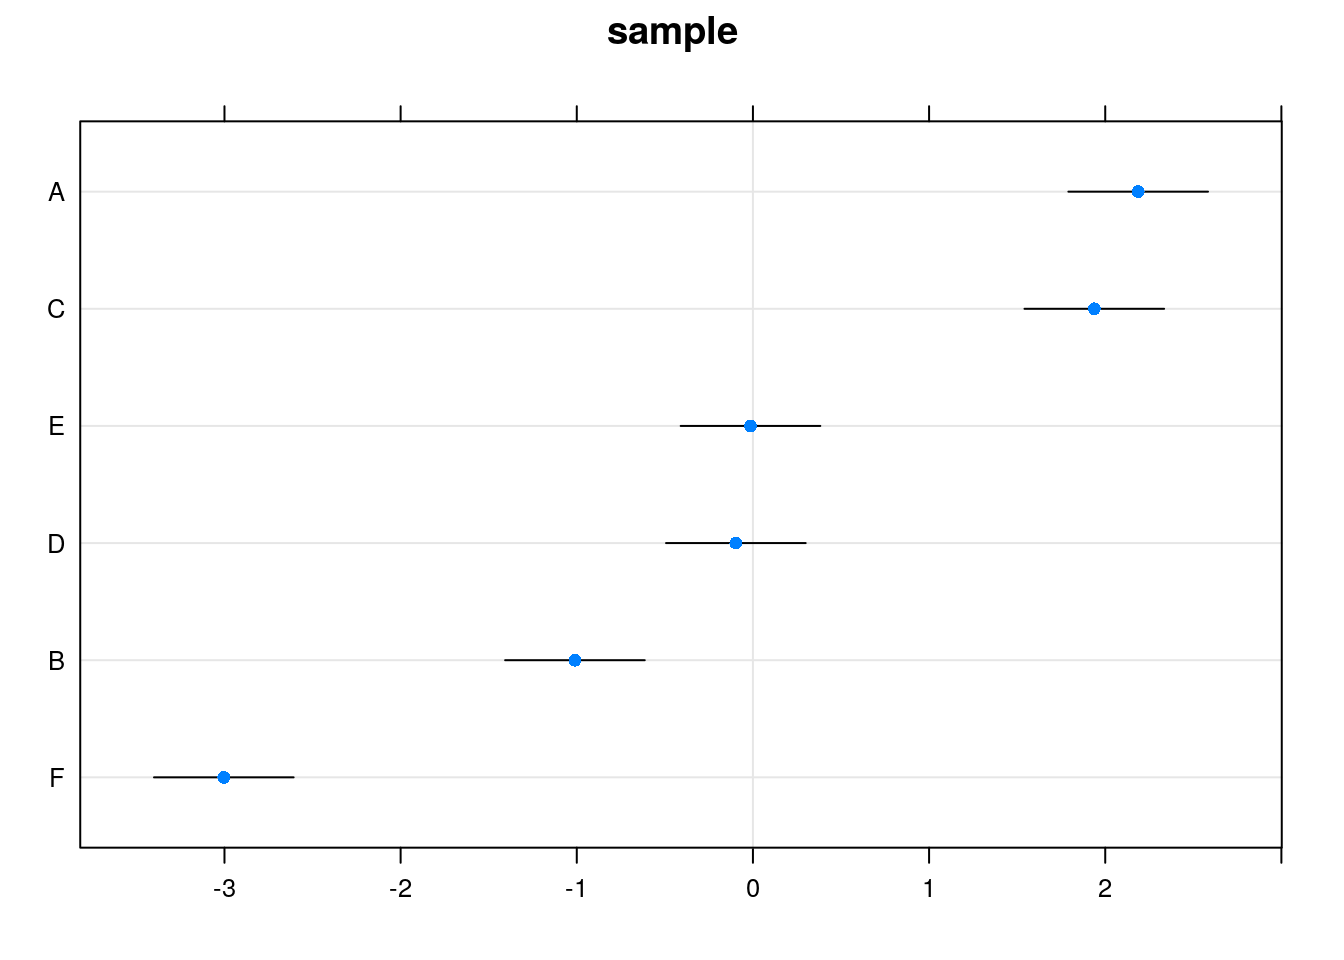
\includegraphics[width=0.5\linewidth]{Rcourse_files/figure-latex/unnamed-chunk-186-1}

Let's fit a logistic regression, and inspect the output.

\begin{Shaded}
\begin{Highlighting}[]
\NormalTok{glm}\FloatTok{.1}\NormalTok{<-}\StringTok{ }\KeywordTok{glm}\NormalTok{(weight.factor}\OperatorTok{~}\NormalTok{group, }\DataTypeTok{family=}\NormalTok{binomial)}
\KeywordTok{summary}\NormalTok{(glm}\FloatTok{.1}\NormalTok{)}
\end{Highlighting}
\end{Shaded}

\begin{verbatim}
## 
## Call:
## glm(formula = weight.factor ~ group, family = binomial)
## 
## Deviance Residuals: 
##     Min       1Q   Median       3Q      Max  
## -2.1460  -0.6681   0.4590   0.8728   1.7941  
## 
## Coefficients:
##             Estimate Std. Error z value Pr(>|z|)  
## (Intercept)   0.4055     0.6455   0.628   0.5299  
## grouptrt1    -1.7918     1.0206  -1.756   0.0792 .
## grouptrt2     1.7918     1.2360   1.450   0.1471  
## ---
## Signif. codes:  0 '***' 0.001 '**' 0.01 '*' 0.05 '.' 0.1 ' ' 1
## 
## (Dispersion parameter for binomial family taken to be 1)
## 
##     Null deviance: 41.054  on 29  degrees of freedom
## Residual deviance: 29.970  on 27  degrees of freedom
## AIC: 35.97
## 
## Number of Fisher Scoring iterations: 4
\end{verbatim}

Things to note:

\begin{itemize}
\tightlist
\item
  The \texttt{glm} function is our workhorse for all GLM models.
\item
  The \texttt{family} argument of \texttt{glm} tells R the respose variable is brenoulli, thus, performing a logistic regression.
\item
  The \texttt{summary} function is content aware. It gives a different output for \texttt{glm} class objects than for other objects, such as the \texttt{lm} we saw in Chapter \ref{lm}. In fact, what \texttt{summary} does is merely call \texttt{summary.glm}.
\item
  As usual, we get the coefficients table, but recall that they are to be interpreted as (log) odd-ratios, i.e., in ``link scale''. To return to probabilities (``response scale''), we will need to undo the logistic transformation.
\item
  As usual, we get the significance for the test of no-effect, versus a two-sided alternative. P-values are asymptotic, thus, only approximate (and can be very bad approximations in small samples).
\item
  The residuals of \texttt{glm} are slightly different than the \texttt{lm} residuals, and called \emph{Deviance Residuals}.
\item
  For help see \texttt{?glm}, \texttt{?family}, and \texttt{?summary.glm}.
\end{itemize}

Like in the linear models, we can use an ANOVA table to check if treatments have any effect, and not one treatment at a time.
In the case of GLMs, this is called an \emph{analysis of deviance} table.

\begin{Shaded}
\begin{Highlighting}[]
\KeywordTok{anova}\NormalTok{(glm}\FloatTok{.1}\NormalTok{, }\DataTypeTok{test=}\StringTok{'LRT'}\NormalTok{)}
\end{Highlighting}
\end{Shaded}

\begin{verbatim}
## Analysis of Deviance Table
## 
## Model: binomial, link: logit
## 
## Response: weight.factor
## 
## Terms added sequentially (first to last)
## 
## 
##       Df Deviance Resid. Df Resid. Dev Pr(>Chi)   
## NULL                     29     41.054            
## group  2   11.084        27     29.970 0.003919 **
## ---
## Signif. codes:  0 '***' 0.001 '**' 0.01 '*' 0.05 '.' 0.1 ' ' 1
\end{verbatim}

Things to note:

\begin{itemize}
\tightlist
\item
  The \texttt{anova} function, like the \texttt{summary} function, are content-aware and produce a different output for the \texttt{glm} class than for the \texttt{lm} class. All that \texttt{anova} does is call \texttt{anova.glm}.
\item
  In GLMs there is no canonical test (like the F test for \texttt{lm}). \texttt{LRT} implies we want an approximate Likelihood Ratio Test.
  We thus specify the type of test desired with the \texttt{test} argument.
\item
  The distribution of the weights of the plants does vary with the treatment given, as we may see from the significance of the \texttt{group} factor.
\item
  Readers familiar with ANOVA tables, should know that we computed the GLM equivalent of a type I sum- of-squares.
  Run \texttt{drop1(glm.1,\ test=\textquotesingle{}Chisq\textquotesingle{})} for a GLM equivalent of a type III sum-of-squares.
\item
  For help see \texttt{?anova.glm}.
\end{itemize}

Let's predict the probability of a heavy plant for each treatment.

\begin{Shaded}
\begin{Highlighting}[]
\KeywordTok{predict}\NormalTok{(glm}\FloatTok{.1}\NormalTok{, }\DataTypeTok{type=}\StringTok{'response'}\NormalTok{)}
\end{Highlighting}
\end{Shaded}

\begin{verbatim}
##   1   2   3   4   5   6   7   8   9  10  11  12  13  14  15  16  17  18 
## 0.6 0.6 0.6 0.6 0.6 0.6 0.6 0.6 0.6 0.6 0.2 0.2 0.2 0.2 0.2 0.2 0.2 0.2 
##  19  20  21  22  23  24  25  26  27  28  29  30 
## 0.2 0.2 0.9 0.9 0.9 0.9 0.9 0.9 0.9 0.9 0.9 0.9
\end{verbatim}

Things to note:

\begin{itemize}
\tightlist
\item
  Like the \texttt{summary} and \texttt{anova} functions, the \texttt{predict} function is aware that its input is of \texttt{glm} class. All that \texttt{predict} does is call \texttt{predict.glm}.
\item
  In GLMs there are many types of predictions. The \texttt{type} argument controls which type is returned. Use \texttt{type=response} for predictions in probability scale; use `type=link' for predictions in log-odds scale.
\item
  How do I know we are predicting the probability of a heavy plant, and not a light plant? Just run \texttt{contrasts(weight.factor)} to see which of the categories of the factor \texttt{weight.factor} is encoded as 1, and which as 0.
\item
  For help see \texttt{?predict.glm}.
\end{itemize}

Let's detach the data so it is no longer in our workspace, and object names do not collide.

\begin{Shaded}
\begin{Highlighting}[]
\KeywordTok{detach}\NormalTok{(PlantGrowth)}
\end{Highlighting}
\end{Shaded}

We gave an example with a factorial (i.e.~discrete) predictor.
We can do the same with multiple continuous predictors.

\begin{Shaded}
\begin{Highlighting}[]
\KeywordTok{data}\NormalTok{(}\StringTok{'Pima.te'}\NormalTok{, }\DataTypeTok{package=}\StringTok{'MASS'}\NormalTok{) }\CommentTok{# Loads data}
\KeywordTok{head}\NormalTok{(Pima.te)}
\end{Highlighting}
\end{Shaded}

\begin{verbatim}
##   npreg glu bp skin  bmi   ped age type
## 1     6 148 72   35 33.6 0.627  50  Yes
## 2     1  85 66   29 26.6 0.351  31   No
## 3     1  89 66   23 28.1 0.167  21   No
## 4     3  78 50   32 31.0 0.248  26  Yes
## 5     2 197 70   45 30.5 0.158  53  Yes
## 6     5 166 72   19 25.8 0.587  51  Yes
\end{verbatim}

\begin{Shaded}
\begin{Highlighting}[]
\NormalTok{glm}\FloatTok{.2}\NormalTok{<-}\StringTok{ }\KeywordTok{step}\NormalTok{(}\KeywordTok{glm}\NormalTok{(type}\OperatorTok{~}\NormalTok{., }\DataTypeTok{data=}\NormalTok{Pima.te, }\DataTypeTok{family=}\KeywordTok{binomial}\NormalTok{(}\DataTypeTok{link=}\StringTok{'probit'}\NormalTok{)))}
\end{Highlighting}
\end{Shaded}

\begin{verbatim}
## Start:  AIC=302.41
## type ~ npreg + glu + bp + skin + bmi + ped + age
## 
##         Df Deviance    AIC
## - bp     1   286.92 300.92
## - skin   1   286.94 300.94
## - age    1   287.74 301.74
## <none>       286.41 302.41
## - ped    1   291.06 305.06
## - npreg  1   292.55 306.55
## - bmi    1   294.52 308.52
## - glu    1   342.35 356.35
## 
## Step:  AIC=300.92
## type ~ npreg + glu + skin + bmi + ped + age
## 
##         Df Deviance    AIC
## - skin   1   287.50 299.50
## - age    1   287.92 299.92
## <none>       286.92 300.92
## - ped    1   291.70 303.70
## - npreg  1   293.06 305.06
## - bmi    1   294.55 306.55
## - glu    1   342.41 354.41
## 
## Step:  AIC=299.5
## type ~ npreg + glu + bmi + ped + age
## 
##         Df Deviance    AIC
## - age    1   288.47 298.47
## <none>       287.50 299.50
## - ped    1   292.41 302.41
## - npreg  1   294.21 304.21
## - bmi    1   304.37 314.37
## - glu    1   343.48 353.48
## 
## Step:  AIC=298.47
## type ~ npreg + glu + bmi + ped
## 
##         Df Deviance    AIC
## <none>       288.47 298.47
## - ped    1   293.78 301.78
## - bmi    1   305.17 313.17
## - npreg  1   305.49 313.49
## - glu    1   349.25 357.25
\end{verbatim}

\begin{Shaded}
\begin{Highlighting}[]
\KeywordTok{summary}\NormalTok{(glm}\FloatTok{.2}\NormalTok{)}
\end{Highlighting}
\end{Shaded}

\begin{verbatim}
## 
## Call:
## glm(formula = type ~ npreg + glu + bmi + ped, family = binomial(link = "probit"), 
##     data = Pima.te)
## 
## Deviance Residuals: 
##     Min       1Q   Median       3Q      Max  
## -2.9935  -0.6487  -0.3585   0.6326   2.5791  
## 
## Coefficients:
##              Estimate Std. Error z value Pr(>|z|)    
## (Intercept) -5.445143   0.569373  -9.563  < 2e-16 ***
## npreg        0.102410   0.025607   3.999 6.35e-05 ***
## glu          0.021739   0.002988   7.276 3.45e-13 ***
## bmi          0.048709   0.012291   3.963 7.40e-05 ***
## ped          0.534366   0.250584   2.132    0.033 *  
## ---
## Signif. codes:  0 '***' 0.001 '**' 0.01 '*' 0.05 '.' 0.1 ' ' 1
## 
## (Dispersion parameter for binomial family taken to be 1)
## 
##     Null deviance: 420.30  on 331  degrees of freedom
## Residual deviance: 288.47  on 327  degrees of freedom
## AIC: 298.47
## 
## Number of Fisher Scoring iterations: 5
\end{verbatim}

Things to note:

\begin{itemize}
\tightlist
\item
  We used the \texttt{\textasciitilde{}.} syntax to tell R to fit a model with all the available predictors.
\item
  Since we want to focus on significant predictors, we used the \texttt{step} function to perform a \emph{step-wise} regression, i.e.~sequentially remove non-significant predictors.
  The function reports each model it has checked, and the variable it has decided to remove at each step.
\item
  The output of \texttt{step} is a single model, with the subset of selected predictors.
\end{itemize}

\hypertarget{poisson-regression}{%
\section{Poisson Regression}\label{poisson-regression}}

Poisson regression means we fit a model assuming \(y|x \sim Poisson(\lambda(x))\).
Put differently, we assume that for each treatment, encoded as a combinations of predictors \(x\), the response is Poisson distributed with a rate that depends on the predictors.

The typical link function for Poisson regression is the logarithm: \(g(t)=log(t)\).
This means that we assume \(y|x \sim Poisson(\lambda(x) = e^{x'\beta})\).
Why is this a good choice?
We again resort to the two-group case, encoded by \(x=1\) and \(x=0\), to understand this model:
\(\lambda(x=1)=e^{\beta_0+\beta_1}=e^{\beta_0} \; e^{\beta_1}= \lambda(x=0) \; e^{\beta_1}\).
We thus see that this link function implies that a change in \(x\) \textbf{multiples} the rate of events by \(e^{\beta_1}\).

For our example\footnote{Taken from \url{http://www.theanalysisfactor.com/generalized-linear-models-in-r-part-6-poisson-regression-count-variables/}} we inspect the number of infected high-school kids, as a function of the days since an outbreak.

\begin{Shaded}
\begin{Highlighting}[]
\NormalTok{cases <-}\StringTok{  }
\KeywordTok{structure}\NormalTok{(}\KeywordTok{list}\NormalTok{(}\DataTypeTok{Days =} \KeywordTok{c}\NormalTok{(1L, 2L, 3L, 3L, 4L, 4L, 4L, 6L, 7L, 8L, }
\NormalTok{8L, 8L, 8L, 12L, 14L, 15L, 17L, 17L, 17L, 18L, 19L, 19L, 20L, }
\NormalTok{23L, 23L, 23L, 24L, 24L, 25L, 26L, 27L, 28L, 29L, 34L, 36L, 36L, }
\NormalTok{42L, 42L, 43L, 43L, 44L, 44L, 44L, 44L, 45L, 46L, 48L, 48L, 49L, }
\NormalTok{49L, 53L, 53L, 53L, 54L, 55L, 56L, 56L, 58L, 60L, 63L, 65L, 67L, }
\NormalTok{67L, 68L, 71L, 71L, 72L, 72L, 72L, 73L, 74L, 74L, 74L, 75L, 75L, }
\NormalTok{80L, 81L, 81L, 81L, 81L, 88L, 88L, 90L, 93L, 93L, 94L, 95L, 95L, }
\NormalTok{95L, 96L, 96L, 97L, 98L, 100L, 101L, 102L, 103L, 104L, 105L, }
\NormalTok{106L, 107L, 108L, 109L, 110L, 111L, 112L, 113L, 114L, 115L), }
    \DataTypeTok{Students =} \KeywordTok{c}\NormalTok{(6L, 8L, 12L, 9L, 3L, 3L, 11L, 5L, 7L, 3L, 8L, }
\NormalTok{    4L, 6L, 8L, 3L, 6L, 3L, 2L, 2L, 6L, 3L, 7L, 7L, 2L, 2L, 8L, }
\NormalTok{    3L, 6L, 5L, 7L, 6L, 4L, 4L, 3L, 3L, 5L, 3L, 3L, 3L, 5L, 3L, }
\NormalTok{    5L, 6L, 3L, 3L, 3L, 3L, 2L, 3L, 1L, 3L, 3L, 5L, 4L, 4L, 3L, }
\NormalTok{    5L, 4L, 3L, 5L, 3L, 4L, 2L, 3L, 3L, 1L, 3L, 2L, 5L, 4L, 3L, }
\NormalTok{    0L, 3L, 3L, 4L, 0L, 3L, 3L, 4L, 0L, 2L, 2L, 1L, 1L, 2L, 0L, }
\NormalTok{    2L, 1L, 1L, 0L, 0L, 1L, 1L, 2L, 2L, 1L, 1L, 1L, 1L, 0L, 0L, }
\NormalTok{    0L, 1L, 1L, 0L, 0L, 0L, 0L, 0L)), }\DataTypeTok{.Names =} \KeywordTok{c}\NormalTok{(}\StringTok{"Days"}\NormalTok{, }\StringTok{"Students"}
\NormalTok{), }\DataTypeTok{class =} \StringTok{"data.frame"}\NormalTok{, }\DataTypeTok{row.names =} \KeywordTok{c}\NormalTok{(}\OtherTok{NA}\NormalTok{, }\OperatorTok{-}\NormalTok{109L))}
\KeywordTok{attach}\NormalTok{(cases)}
\KeywordTok{head}\NormalTok{(cases) }
\end{Highlighting}
\end{Shaded}

\begin{verbatim}
##   Days Students
## 1    1        6
## 2    2        8
## 3    3       12
## 4    3        9
## 5    4        3
## 6    4        3
\end{verbatim}

Look at the following plot and think:

\begin{itemize}
\tightlist
\item
  Can we assume that the errors have constant variance?
\item
  What is the sign of the effect of time on the number of sick students?
\item
  Can we assume a linear effect of time?
\end{itemize}

\begin{Shaded}
\begin{Highlighting}[]
\KeywordTok{plot}\NormalTok{(Days, Students, }\DataTypeTok{xlab =} \StringTok{"DAYS"}\NormalTok{, }\DataTypeTok{ylab =} \StringTok{"STUDENTS"}\NormalTok{, }\DataTypeTok{pch =} \DecValTok{16}\NormalTok{)}
\end{Highlighting}
\end{Shaded}

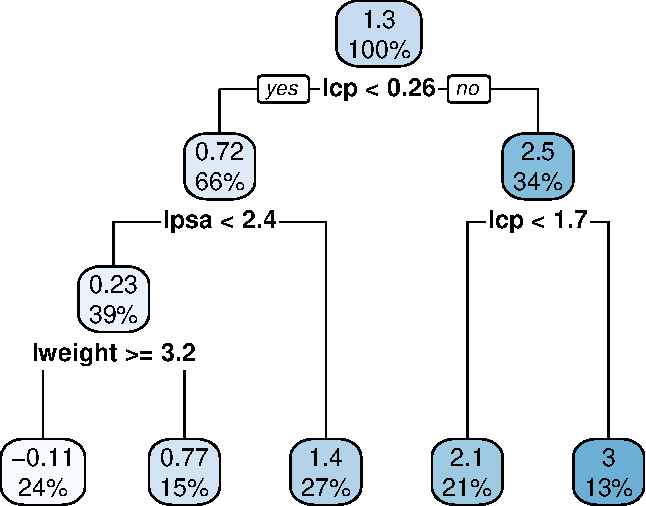
\includegraphics[width=0.5\linewidth]{Rcourse_files/figure-latex/unnamed-chunk-193-1}

We now fit a model to check for the change in the rate of events as a function of the days since the outbreak.

\begin{Shaded}
\begin{Highlighting}[]
\NormalTok{glm}\FloatTok{.3}\NormalTok{ <-}\StringTok{ }\KeywordTok{glm}\NormalTok{(Students }\OperatorTok{~}\StringTok{ }\NormalTok{Days, }\DataTypeTok{family =}\NormalTok{ poisson)}
\KeywordTok{summary}\NormalTok{(glm}\FloatTok{.3}\NormalTok{)}
\end{Highlighting}
\end{Shaded}

\begin{verbatim}
## 
## Call:
## glm(formula = Students ~ Days, family = poisson)
## 
## Deviance Residuals: 
##      Min        1Q    Median        3Q       Max  
## -2.00482  -0.85719  -0.09331   0.63969   1.73696  
## 
## Coefficients:
##              Estimate Std. Error z value Pr(>|z|)    
## (Intercept)  1.990235   0.083935   23.71   <2e-16 ***
## Days        -0.017463   0.001727  -10.11   <2e-16 ***
## ---
## Signif. codes:  0 '***' 0.001 '**' 0.01 '*' 0.05 '.' 0.1 ' ' 1
## 
## (Dispersion parameter for poisson family taken to be 1)
## 
##     Null deviance: 215.36  on 108  degrees of freedom
## Residual deviance: 101.17  on 107  degrees of freedom
## AIC: 393.11
## 
## Number of Fisher Scoring iterations: 5
\end{verbatim}

Things to note:

\begin{itemize}
\tightlist
\item
  We used \texttt{family=poisson} in the \texttt{glm} function to tell R that we assume a Poisson distribution.
\item
  The coefficients table is there as usual.
  When interpreting the table, we need to recall that the effect, i.e.~the \(\hat \beta\), are \textbf{multiplicative} due to the assumed link function.
\item
  Each day \textbf{decreases} the rate of events by a factor of about \(e^{\beta_1}=\) 0.98.
\item
  For more information see \texttt{?glm} and \texttt{?family}.
\end{itemize}

\hypertarget{extensions}{%
\section{Extensions}\label{extensions}}

As we already implied, GLMs are a very wide class of models.
We do not need to use the default link function,but more importantly, we are not constrained to Binomial, or Poisson distributed response.
For exponential, gamma, and other response distributions, see \texttt{?glm} or the references in the Bibliographic Notes section.

\hypertarget{bibliographic-notes-5}{%
\section{Bibliographic Notes}\label{bibliographic-notes-5}}

The ultimate reference on GLMs is \citet{mccullagh1984generalized}.
For a less technical exposition, we refer to the usual \citet{venables2013modern}.

\hypertarget{practice-glm}{%
\section{Practice Yourself}\label{practice-glm}}

\begin{enumerate}
\def\labelenumi{\arabic{enumi}.}
\item
  Try using \texttt{lm} for analyzing the plant growth data in \texttt{weight.factor} as a function of \texttt{group} in the \texttt{PlantGrowth} data.
\item
  Generate some synthetic data for a logistic regression:

  \begin{enumerate}
  \def\labelenumii{\alph{enumii}.}
  \tightlist
  \item
    Generate two predictor variables of length \(100\). They can be random from your favorite distribution.
  \item
    Fix \texttt{beta\textless{}-\ c(-1,2)}, and generate the response with:\texttt{rbinom(n=100,size=1,prob=exp(x\ \%*\%\ beta)/(1+exp(x\ \%*\%\ beta)))}. Think: why is this the model implied by the logistic regression?
  \item
    Fit a Logistic regression to your synthetic data using \texttt{glm}.
  \item
    Are the estimated coefficients similar to the true ones you used?
  \item
    What is the estimated probability of an event at \texttt{x=1,1}? Use \texttt{predict.glm} but make sure to read the documentation on the \texttt{type} argument.
  \end{enumerate}
\item
  Read about the \texttt{epil} dataset using \texttt{?\ MASS::epil}. Inspect the dependency of the number of seizures (\(y\)) in the age of the patient (\texttt{age}) and the treatment (\texttt{trt}).

  \begin{enumerate}
  \def\labelenumii{\arabic{enumii}.}
  \tightlist
  \item
    Fit a Poisson regression with \texttt{glm} and \texttt{family\ =\ "poisson"}.
  \item
    Are the coefficients significant?\\
  \item
    Does the treatment reduce the frequency of the seizures?
  \item
    According to this model, what would be the number of seizures for 20 years old patient with progabide treatment?
  \end{enumerate}
\end{enumerate}

See DataCamp's \href{https://www.datacamp.com/courses/generalized-linear-models-in-r}{Generalized Linear Models in R} for more self practice.

\hypertarget{lme}{%
\chapter{Linear Mixed Models}\label{lme}}

\BeginKnitrBlock{example}[Dependent Samples on the Mean]
\protect\hypertarget{exm:dependence}{}{\label{exm:dependence} \iffalse (Dependent Samples on the Mean) \fi{} }Consider inference on a population's mean.
Supposdly, more observations imply more infotmation on the mean. This, however, is not the case if samples are completely dependant. More observations do not add any new information.
From this example one may think that dependence is a bad thing. This is a false intuitiont: negative correlations imply oscilations about the mean, so they are actually more informative on the mean than independent observations.
\EndKnitrBlock{example}

\BeginKnitrBlock{example}[Repeated Measures]
\protect\hypertarget{exm:repeated-measures}{}{\label{exm:repeated-measures} \iffalse (Repeated Measures) \fi{} }Consider a prospective study, i.e., data that originates from selecting a set of subjects and making measurements on them over time.
Also assume that some subjects received some treatment, and other did not.
When we want to infer on the population from which these subjects have been sampled, we need to recall that some series of observations came from the same subject.
If we were to ignore the subject of origin, and treat each observation as an independent sample point, we will think we have more information in our data than we actually do.
For a rough intuition, think of a case where observatiosn within subject are perfectly dependent.
\EndKnitrBlock{example}

The sources of variability, i.e.~noise, are known in the statistical literature as ``random effects''.
Specifying these sources determines the correlation structure in our measurements.
In the simplest linear models of Chapter \ref{lm}, we thought of the variability as a measurement error, independent of anything else. This, however, is rarely the case when time or space are involved.

The variability in our data is rarely the object of interest.
It is merely the source of uncertainty in our measurements.
The effects we want to infer on are assumingly non-random, thus known as ``fixed-effects''.
A model which has several sources of variability, i.e.~random-effects, and several deterministic effects to study, i.e.~fixed-effects, is known as a ``mixed effects'' model.
If the model is also linear, it is known as a \emph{linear mixed model} (LMM).
Here are some examples of such models.

\BeginKnitrBlock{example}[Fixed and Random Machine Effect]
\protect\hypertarget{exm:fixed-effects}{}{\label{exm:fixed-effects} \iffalse (Fixed and Random Machine Effect) \fi{} }Consider the problem of testing for a change in the distribution of diamteters of manufactured bottle caps.
We want to study the (fixed) effect of time: before versus after.
Bottle caps are produced by several machines.
Clearly there is variablity in the diameters within-machine and between-machines.
Given many measurements on many bottle caps from many machines, we could standardize measurements by removing each machine's average.
This implies the within-machine variability is the only source of variability we care about, because the substration of the machine effect, removed information on the between-machine variability.\\
Alternatively, we could treat the between-machine variability as another source of noise/uncertainty when inferring on the temporal fixed effect.
\EndKnitrBlock{example}

\BeginKnitrBlock{example}[Fixed and Random Subject Effect]
\protect\hypertarget{exm:random-effects}{}{\label{exm:random-effects} \iffalse (Fixed and Random Subject Effect) \fi{} }Consider an experimenal design where each subject is given 2 types of diets, and his health condition is recorded.
We could standardize over subjects by removing the subject-wise average, before comparing diets.
This is what a paired t-test does.
This also implies the within-subject variability is the only source of variability we care about.
Alternatively, for inference on the population of ``all subjects'' we need to adress the between-subject variability, and not only the within-subject variability.
\EndKnitrBlock{example}

The unifying theme of the above examples, is that the variability in our data has several sources.
Which are the sources of variability that need to concern us?
This is a delicate matter which depends on your goals.
As a rule of thumb, we will suggest the following view:
\textbf{If information of an effect will be available at the time of prediction, treat it as a fixed effect. If it is not, treat it as a random-effect.}

LMMs are so fundamental, that they have earned many names:

\begin{itemize}
\item
  \textbf{Mixed Effects}:
  Because we may have both \emph{fixed effects} we want to estimate and remove, and \emph{random effects} which contribute to the variability to infer against.
\item
  \textbf{Variance Components}:
  Because as the examples show, variance has more than a single source (like in the Linear Models of Chapter \ref{lm}).
\item
  \textbf{Hirarchial Models}:
  Because as Example \ref{exm:random-effects} demonstrates, we can think of the sampling as hierarchical-- first sample a subject, and then sample its response.
\item
  \textbf{Multilevel Analysis}:
  For the same reasons it is also known as Hierarchical Models.
\item
  \textbf{Repeated Measures}:
  Because we make several measurements from each unit, like in Example \ref{exm:random-effects}.
\item
  \textbf{Longitudinal Data}:
  Because we follow units over time, like in Example \ref{exm:random-effects}.
\item
  \textbf{Panel Data}:
  Is the term typically used in econometric for such longitudinal data.
\item
  \textbf{MANOVA}:
  Many of the problems that may be solved with a multivariate analysis of variance (MANOVA), may be solved with an LMM for reasons we detail in \ref{multivariate}.
\item
  \textbf{Structured Prediction}:
  In the machine learning literature, predicting outcomes with structure, such as correlated vectors, is known as Structured Learning.
  Because LMMs merely specify correlations, using a LMM for making predictions may be thought of as an instance of structured prediction.
\end{itemize}

Whether we are aiming to infer on a generative model's parameters, or to make predictions, there is no ``right'' nor ``wrong'' approach. Instead, there is always some implied measure of error, and an algorithm may be good, or bad, with respect to this measure (think of false and true positives, for instance).
This is why we care about dependencies in the data: ignoring the dependence structure will probably yield inefficient algorithms.
Put differently, if we ignore the statistical dependence in the data we will probably me making more errors than possible/optimal.

We now emphasize:

\begin{enumerate}
\def\labelenumi{\arabic{enumi}.}
\item
  Like in previous chapters, by ``model'' we refer to the assumed generative distribution, i.e., the sampling distribution.
\item
  LMMs are a way to infer against the right level of variability.
  Using a naive linear model (which assumes a single source of variability) instead of a mixed effects model, probably means your inference is overly anti-conservative.
  Put differently, the uncertainty in your estimates is higher than the linear model from Chapter \ref{lm} may suggest.
\item
  In a LMM we will specify the dependence structure via the hierarchy in the sampling scheme (e.g.~caps within machine, students within class, etc.).
  Not all dependency models can be specified in this way.
  Dependency structures that are not hierarchical include temporal dependencies (\href{https://en.wikipedia.org/wiki/Autoregressive_model}{AR}, \href{https://en.wikipedia.org/wiki/Autoregressive_integrated_moving_average}{ARIMA}, \href{https://en.wikipedia.org/wiki/Autoregressive_conditional_heteroskedasticity}{ARCH} and GARCH), \href{https://en.wikipedia.org/wiki/Spatial_dependence}{spatial}, \href{https://en.wikipedia.org/wiki/Markov_chain}{Markov Chains}, and more.
  To specify dependency structures that are no hierarchical, see Chapter 8 in (the excellent) \citet{weiss2005modeling}.
\item
  If you are using the model merely for predictions, and not for inference on the fixed effects or variance components, then stating the generative distribution may be be useful, but not necessarily.
  See the Supervised Learning Chapter \ref{supervised} for more on prediction problems.
  Also recall that machine learning from non-independent observations (such as LMMs) is a delicate matter that is rarely treated in the literature.
\end{enumerate}

\hypertarget{problem-setup-2}{%
\section{Problem Setup}\label{problem-setup-2}}

\begin{align}
  y|x,u = x'\beta + z'u + \varepsilon
  \label{eq:mixed-model}  
\end{align}
where \(x\) are the factors with fixed effects, \(\beta\), which we may want to study.
The factors \(z\), with effects \(u\), are the random effects which contribute to variability.
In our repeated measures example (\ref{exm:repeated-measures}) the treatment is a fixed effect, and the subject is a random effect.
In our bottle-caps example (\ref{exm:fixed-effects}) the time (before vs.~after) is a fixed effect, and the machines may be either a fixed or a random effect (depending on the purpose of inference).
In our diet example (\ref{exm:random-effects}) the diet is the fixed effect and the family is a random effect.

Notice that we state \(y|x,z\) merely as a convenient way to do inference on \(y|x\), instead of directly specifying \(Var[y|x]\).
This is exactly the power of LMMs: we specify the covariance not via the matrix \(Var[y,z]\), but rather via the sampling hierarchy.

Given a sample of \(n\) observations \((y_i,x_i,z_i)\) from model \eqref{eq:mixed-model}, we will want to estimate \((\beta,u)\).
Under some assumption on the distribution of \(\varepsilon\) and \(z\), we can use \emph{maximum likelihood} (ML).
In the context of LMMs, however, ML is typically replaced with \emph{restricted maximum likelihood} (ReML), because it returns unbiased estimates of \(Var[y|x]\) and ML does not.

\hypertarget{non-linear-mixed-models}{%
\subsection{Non-Linear Mixed Models}\label{non-linear-mixed-models}}

The idea of random-effects can also be implemented for non-linear mean models. Formally, this means that \(y|x,z=f(x,z,\varepsilon)\) for some non-linear \(f\).
This is known as \emph{non-linead-mixed-models}, which will not be discussed in this text.

\hypertarget{generalized-linear-mixed-models-glmm}{%
\subsection{Generalized Linear Mixed Models (GLMM)}\label{generalized-linear-mixed-models-glmm}}

You can marry the ideas of random effects, with non-linear link functions, and non-Gaussian distribution of the response.
These are known as \href{https://en.wikipedia.org/wiki/Generalized_linear_mixed_model}{Generalized Linear Mixed Models}.
\href{http://glmm.wikidot.com/pkg-comparison}{Wikidot} has a nice comparison of several software suits for GLMMs.
Also consider the \href{https://www.jstatsoft.org/article/view/v084i04}{mcglm} R pacakge \citep{bonat2018multiple}.

\hypertarget{mixed-models-with-r}{%
\section{Mixed Models with R}\label{mixed-models-with-r}}

We will fit mixed models with the \texttt{lmer} function from the \textbf{lme4} package, written by the mixed-models Guru \href{http://www.stat.wisc.edu/~bates/}{Douglas Bates}.
We start with a small simulation demonstrating the importance of acknowledging your sources of variability. Our demonstration consists of fitting a linear model that assumes independence, when data is clearly dependent.

\begin{Shaded}
\begin{Highlighting}[]
\CommentTok{# Simulation parameters}
\NormalTok{n.groups <-}\StringTok{ }\DecValTok{4} \CommentTok{# number of groups}
\NormalTok{n.repeats <-}\StringTok{ }\DecValTok{2} \CommentTok{# sample per group}
\NormalTok{groups <-}\StringTok{ }\KeywordTok{rep}\NormalTok{(}\DecValTok{1}\OperatorTok{:}\NormalTok{n.groups, }\DataTypeTok{each=}\NormalTok{n.repeats) }\OperatorTok\StringTok{ }\NormalTok{as.factor}
\NormalTok{n <-}\StringTok{ }\KeywordTok{length}\NormalTok{(groups)}
\NormalTok{z0 <-}\StringTok{ }\KeywordTok{rnorm}\NormalTok{(n.groups,}\DecValTok{0}\NormalTok{,}\DecValTok{10}\NormalTok{) }\CommentTok{# generate group effects}
\NormalTok{(z <-}\StringTok{ }\NormalTok{z0[}\KeywordTok{as.numeric}\NormalTok{(groups)]) }\CommentTok{# generate and inspect random group effects}
\end{Highlighting}
\end{Shaded}

\begin{verbatim}
## [1]   8.901364   8.901364  -4.318889  -4.318889   9.708611   9.708611
## [7] -10.693773 -10.693773
\end{verbatim}

\begin{Shaded}
\begin{Highlighting}[]
\NormalTok{epsilon <-}\StringTok{ }\KeywordTok{rnorm}\NormalTok{(n,}\DecValTok{0}\NormalTok{,}\DecValTok{1}\NormalTok{) }\CommentTok{# generate measurement error}

\CommentTok{# Generate data}
\NormalTok{beta0 <-}\StringTok{ }\DecValTok{2} \CommentTok{# set global mean}
\NormalTok{y <-}\StringTok{ }\NormalTok{beta0 }\OperatorTok{+}\StringTok{ }\NormalTok{z }\OperatorTok{+}\StringTok{ }\NormalTok{epsilon }\CommentTok{# generate synthetic sample}
\end{Highlighting}
\end{Shaded}

We can now fit the linear and mixed models.

\begin{Shaded}
\begin{Highlighting}[]
\NormalTok{lm}\FloatTok{.5}\NormalTok{ <-}\StringTok{ }\KeywordTok{lm}\NormalTok{(y}\OperatorTok{~}\DecValTok{1}\NormalTok{)  }\CommentTok{# fit a linear model assuming independence}
\KeywordTok{library}\NormalTok{(lme4)}
\NormalTok{lme}\FloatTok{.5}\NormalTok{ <-}\StringTok{ }\KeywordTok{lmer}\NormalTok{(y}\OperatorTok{~}\DecValTok{1}\OperatorTok{|}\NormalTok{groups) }\CommentTok{# fit a mixed-model that deals with the group dependence}
\end{Highlighting}
\end{Shaded}

The summary of the linear model

\begin{Shaded}
\begin{Highlighting}[]
\NormalTok{summary.lm}\FloatTok{.5}\NormalTok{ <-}\StringTok{ }\KeywordTok{summary}\NormalTok{(lm}\FloatTok{.5}\NormalTok{)}
\NormalTok{summary.lm}\FloatTok{.5}
\end{Highlighting}
\end{Shaded}

\begin{verbatim}
## 
## Call:
## lm(formula = y ~ 1)
## 
## Residuals:
##     Min      1Q  Median      3Q     Max 
## -13.949  -7.275   1.629   8.668  10.005 
## 
## Coefficients:
##             Estimate Std. Error t value Pr(>|t|)
## (Intercept)    3.317      3.500   0.948    0.375
## 
## Residual standard error: 9.898 on 7 degrees of freedom
\end{verbatim}

The summary of the mixed-model

\begin{Shaded}
\begin{Highlighting}[]
\NormalTok{summary.lme}\FloatTok{.5}\NormalTok{ <-}\StringTok{ }\KeywordTok{summary}\NormalTok{(lme}\FloatTok{.5}\NormalTok{)}
\NormalTok{summary.lme}\FloatTok{.5}
\end{Highlighting}
\end{Shaded}

\begin{verbatim}
## Linear mixed model fit by REML ['lmerMod']
## Formula: y ~ 1 | groups
## 
## REML criterion at convergence: 41
## 
## Scaled residuals: 
##      Min       1Q   Median       3Q      Max 
## -1.15395 -0.50048  0.04306  0.55891  0.99797 
## 
## Random effects:
##  Groups   Name        Variance Std.Dev.
##  groups   (Intercept) 111.962  10.581  
##  Residual               2.012   1.418  
## Number of obs: 8, groups:  groups, 4
## 
## Fixed effects:
##             Estimate Std. Error t value
## (Intercept)    3.317      5.314   0.624
\end{verbatim}

Look at the standard error of the global mean, i.e., the intercept:
for \texttt{lm} it is 3.4996374, and for \texttt{lme} it is 5.3143284.
Why this difference?
Because \texttt{lm} treats the group effect\footnote{A.k.a. the \emph{cluster effect}.} as a fixed while the mixed model treats the group effect as a source of noise/uncertainty.
Clearly, inference using \texttt{lm} underestimates our uncertainty in the estimated population mean (\(\beta_0\)).

Now let's adopt the paired t-test view, which removes the group mean, so that it implicitly ignores the between-group variability. Which is the model compatible with this view?

\begin{Shaded}
\begin{Highlighting}[]
\NormalTok{diffs <-}\StringTok{ }\KeywordTok{tapply}\NormalTok{(y, groups, diff) }
\NormalTok{diffs }\CommentTok{# Q:what is this estimating? A: epsilon+epsilon.}
\end{Highlighting}
\end{Shaded}

\begin{verbatim}
##         1         2         3         4 
## -1.411024 -1.598983 -1.493730  3.052394
\end{verbatim}

\begin{Shaded}
\begin{Highlighting}[]
\KeywordTok{sd}\NormalTok{(diffs) }\CommentTok{# }
\end{Highlighting}
\end{Shaded}

\begin{verbatim}
## [1] 2.278119
\end{verbatim}

So we see that a paired t-test infers only against the within-group variability.
Q:Is this a good think?
A: depends\ldots{}

\hypertarget{a-single-random-effect}{%
\subsection{A Single Random Effect}\label{a-single-random-effect}}

We will use the \texttt{Dyestuff} data from the \textbf{lme4} package, which encodes the yield, in grams, of a coloring solution (\texttt{dyestuff}), produced in 6 batches using 5 different preparations.

\begin{Shaded}
\begin{Highlighting}[]
\KeywordTok{data}\NormalTok{(Dyestuff, }\DataTypeTok{package=}\StringTok{'lme4'}\NormalTok{)}
\KeywordTok{attach}\NormalTok{(Dyestuff)}
\KeywordTok{head}\NormalTok{(Dyestuff)}
\end{Highlighting}
\end{Shaded}

\begin{verbatim}
##   Batch Yield
## 1     A  1545
## 2     A  1440
## 3     A  1440
## 4     A  1520
## 5     A  1580
## 6     B  1540
\end{verbatim}

And visually

\begin{Shaded}
\begin{Highlighting}[]
\NormalTok{lattice}\OperatorTok{::}\KeywordTok{dotplot}\NormalTok{(Yield}\OperatorTok{~}\NormalTok{Batch)}
\end{Highlighting}
\end{Shaded}

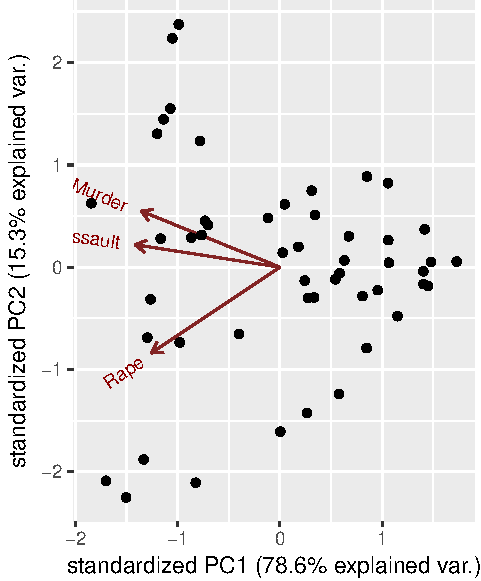
\includegraphics[width=0.5\linewidth]{Rcourse_files/figure-latex/unnamed-chunk-199-1}

If we want to do inference on the (global) mean yield, we need to account for the two sources of variability: the within-batch variability, and the between-batch variability
We thus fit a mixed model, with an intercept and random batch effect.

\begin{Shaded}
\begin{Highlighting}[]
\NormalTok{lme}\FloatTok{.1}\NormalTok{<-}\StringTok{ }\KeywordTok{lmer}\NormalTok{( Yield }\OperatorTok{~}\StringTok{ }\DecValTok{1}  \OperatorTok{|}\StringTok{ }\NormalTok{Batch  , Dyestuff )}
\KeywordTok{summary}\NormalTok{(lme}\FloatTok{.1}\NormalTok{)}
\end{Highlighting}
\end{Shaded}

\begin{verbatim}
## Linear mixed model fit by REML ['lmerMod']
## Formula: Yield ~ 1 | Batch
##    Data: Dyestuff
## 
## REML criterion at convergence: 319.7
## 
## Scaled residuals: 
##     Min      1Q  Median      3Q     Max 
## -1.4117 -0.7634  0.1418  0.7792  1.8296 
## 
## Random effects:
##  Groups   Name        Variance Std.Dev.
##  Batch    (Intercept) 1764     42.00   
##  Residual             2451     49.51   
## Number of obs: 30, groups:  Batch, 6
## 
## Fixed effects:
##             Estimate Std. Error t value
## (Intercept)  1527.50      19.38    78.8
\end{verbatim}

Things to note:

\begin{itemize}
\tightlist
\item
  The syntax \texttt{Yield\ \textasciitilde{}\ 1\ \ \textbar{}\ Batch} tells R to fit a model with a global intercept (\texttt{1}) and a random Batch effect (\texttt{\textbar{}Batch}). More on that later.
\item
  As usual, \texttt{summary} is content aware and has a different behavior for \texttt{lme} class objects.
\item
  The output distinguishes between random effects (\(u\)), a source of variability, and fixed effect (\(\beta\)), which we want to study. The mean of the random effect is not reported because it is unassumingly 0.
\item
  Were we not interested in the variance components, and only in the coefficients or predictions, an (almost) equivalent \texttt{lm} formulation is \texttt{lm(Yield\ \textasciitilde{}\ Batch)}.
\end{itemize}

Some utility functions let us query the \texttt{lme} object.
The function \texttt{coef} will work, but will return a cumbersome output. Better use \texttt{fixef} to extract the fixed effects, and \texttt{ranef} to extract the random effects.
The model matrix (of the fixed effects alone), can be extracted with \texttt{model.matrix}, and predictions made with \texttt{predict}.
Note, however, that predictions with mixed-effect models are better treated as prediction problems as in the Supervised Learning Chapter \ref{supervised}, but are a very delicate matter.

\begin{Shaded}
\begin{Highlighting}[]
\KeywordTok{detach}\NormalTok{(Dyestuff)}
\end{Highlighting}
\end{Shaded}

\hypertarget{multiple-random-effects}{%
\subsection{Multiple Random Effects}\label{multiple-random-effects}}

Let's make things more interesting by allowing more than one random effect.
One-way ANOVA can be thought of as the fixed-effects counterpart of the single random effect.

In the \texttt{Penicillin} data, we measured the diameter of spread of an organism, along the plate used (a to x), and penicillin type (A to F).
We will now try to infer on the diameter of typical organism, and compute its variability over plates and Penicillin types.

\begin{Shaded}
\begin{Highlighting}[]
\KeywordTok{head}\NormalTok{(Penicillin)}
\end{Highlighting}
\end{Shaded}

\begin{verbatim}
##   diameter plate sample
## 1       27     a      A
## 2       23     a      B
## 3       26     a      C
## 4       23     a      D
## 5       23     a      E
## 6       21     a      F
\end{verbatim}

One sample per combination:

\begin{Shaded}
\begin{Highlighting}[]
\KeywordTok{attach}\NormalTok{(Penicillin)}
\KeywordTok{table}\NormalTok{(sample, plate) }\CommentTok{# how many observations per plate & type?}
\end{Highlighting}
\end{Shaded}

\begin{verbatim}
##       plate
## sample a b c d e f g h i j k l m n o p q r s t u v w x
##      A 1 1 1 1 1 1 1 1 1 1 1 1 1 1 1 1 1 1 1 1 1 1 1 1
##      B 1 1 1 1 1 1 1 1 1 1 1 1 1 1 1 1 1 1 1 1 1 1 1 1
##      C 1 1 1 1 1 1 1 1 1 1 1 1 1 1 1 1 1 1 1 1 1 1 1 1
##      D 1 1 1 1 1 1 1 1 1 1 1 1 1 1 1 1 1 1 1 1 1 1 1 1
##      E 1 1 1 1 1 1 1 1 1 1 1 1 1 1 1 1 1 1 1 1 1 1 1 1
##      F 1 1 1 1 1 1 1 1 1 1 1 1 1 1 1 1 1 1 1 1 1 1 1 1
\end{verbatim}

And visually:

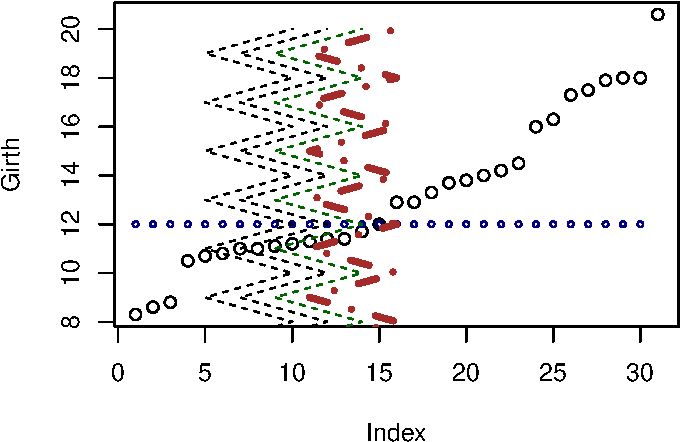
\includegraphics[width=0.5\linewidth]{Rcourse_files/figure-latex/unnamed-chunk-203-1}

Let's fit a mixed-effects model with a random plate effect, and a random sample effect:

\begin{Shaded}
\begin{Highlighting}[]
\NormalTok{lme}\FloatTok{.2}\NormalTok{ <-}\StringTok{ }\KeywordTok{lmer}\NormalTok{ ( diameter }\OperatorTok{~}\StringTok{  }\DecValTok{1}  \OperatorTok{+}\StringTok{ }\NormalTok{(}\DecValTok{1}\OperatorTok{|}\NormalTok{plate )}\OperatorTok{+}\NormalTok{(}\DecValTok{1}\OperatorTok{|}\NormalTok{sample) , Penicillin )}
\KeywordTok{fixef}\NormalTok{(lme}\FloatTok{.2}\NormalTok{) }\CommentTok{# Fixed effects}
\end{Highlighting}
\end{Shaded}

\begin{verbatim}
## (Intercept) 
##    22.97222
\end{verbatim}

\begin{Shaded}
\begin{Highlighting}[]
\KeywordTok{ranef}\NormalTok{(lme}\FloatTok{.2}\NormalTok{) }\CommentTok{# Random effects}
\end{Highlighting}
\end{Shaded}

\begin{verbatim}
## $plate
##   (Intercept)
## a  0.80454389
## b  0.80454389
## c  0.18167120
## d  0.33738937
## e  0.02595303
## f -0.44120149
## g -1.37551052
## h  0.80454389
## i -0.75263783
## j -0.75263783
## k  0.96026206
## l  0.49310755
## m  1.42741658
## n  0.49310755
## o  0.96026206
## p  0.02595303
## q -0.28548332
## r -0.28548332
## s -1.37551052
## t  0.96026206
## u -0.90835601
## v -0.28548332
## w -0.59691966
## x -1.21979235
## 
## $sample
##   (Intercept)
## A  2.18705819
## B -1.01047625
## C  1.93789966
## D -0.09689498
## E -0.01384214
## F -3.00374447
## 
## with conditional variances for "plate" "sample"
\end{verbatim}

Things to note:

\begin{itemize}
\tightlist
\item
  The syntax \texttt{1+\ (1\textbar{}\ plate\ )\ +\ (1\textbar{}\ sample\ )} fits a global intercept (mean), a random plate effect, and a random sample effect.
\item
  Were we not interested in the variance components, an (almost) equivalent \texttt{lm} formulation is \texttt{lm(diameter\ \textasciitilde{}\ plate\ +\ sample)}.
\item
  The output of \texttt{ranef} is somewhat controversial. Think about it: Why would we want to plot the estimates of a random variable?
\end{itemize}

Since we have two random effects, we may compute the variability of the global mean (the only fixed effect) as we did before.
Perhaps more interestingly, we can compute the variability in the response, for a particular plate or sample type.

\begin{Shaded}
\begin{Highlighting}[]
\NormalTok{random.effect.lme2 <-}\StringTok{ }\KeywordTok{ranef}\NormalTok{(lme}\FloatTok{.2}\NormalTok{, }\DataTypeTok{condVar =} \OtherTok{TRUE}\NormalTok{) }
\NormalTok{qrr2 <-}\StringTok{ }\NormalTok{lattice}\OperatorTok{::}\KeywordTok{dotplot}\NormalTok{(random.effect.lme2, }\DataTypeTok{strip =} \OtherTok{FALSE}\NormalTok{)}
\end{Highlighting}
\end{Shaded}

Variability in response for each plate, over various sample types:

\begin{Shaded}
\begin{Highlighting}[]
\KeywordTok{print}\NormalTok{(qrr2[[}\DecValTok{1}\NormalTok{]]) }
\end{Highlighting}
\end{Shaded}

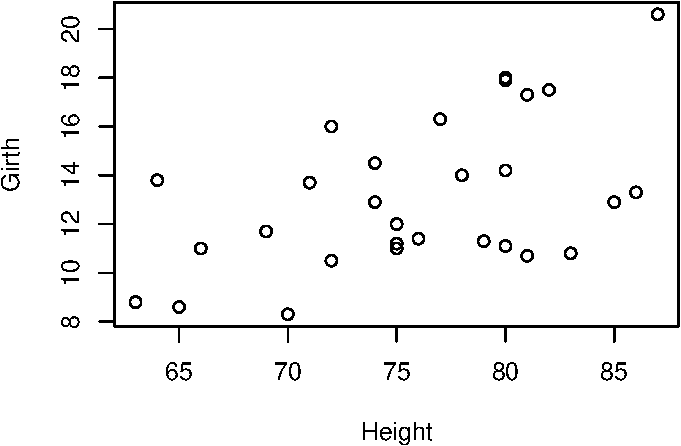
\includegraphics[width=0.5\linewidth]{Rcourse_files/figure-latex/unnamed-chunk-206-1}

Variability in response for each sample type, over the various plates:

\begin{Shaded}
\begin{Highlighting}[]
\KeywordTok{print}\NormalTok{(qrr2[[}\DecValTok{2}\NormalTok{]])  }
\end{Highlighting}
\end{Shaded}

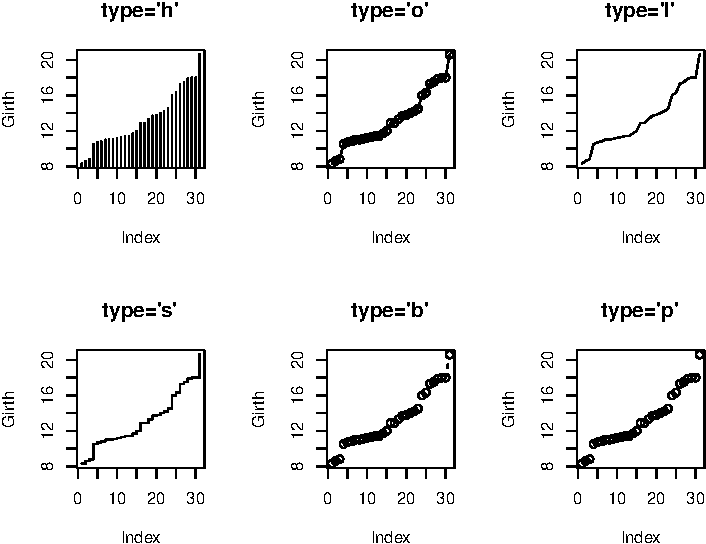
\includegraphics[width=0.5\linewidth]{Rcourse_files/figure-latex/unnamed-chunk-207-1}

Things to note:

\begin{itemize}
\tightlist
\item
  The \texttt{condVar} argument of the \texttt{ranef} function tells R to compute the variability in response conditional on each random effect at a time.
\item
  The \texttt{dotplot} function, from the \textbf{lattice} package, is only there for the fancy plotting.
\end{itemize}

We used the penicillin example to demonstrate the incorporation of two random-effects. We could have, however, compared between penicillin types. For this matter, penicillin types are fixed effects to infer on, and not part of the uncertainty in the mean diameter. The appropriate model is the following:

\begin{Shaded}
\begin{Highlighting}[]
\NormalTok{lme.}\FloatTok{2.2}\NormalTok{ <-}\StringTok{ }\KeywordTok{lmer}\NormalTok{( diameter }\OperatorTok{~}\StringTok{  }\DecValTok{1}  \OperatorTok{+}\StringTok{ }\NormalTok{sample }\OperatorTok{+}\StringTok{ }\NormalTok{(}\DecValTok{1}\OperatorTok{|}\NormalTok{plate) , Penicillin )}
\end{Highlighting}
\end{Shaded}

I may now ask myself: does the \texttt{sample}, i.e.~penicillin, have any effect? This is what the ANOVA table typically gives us. The next table can be thought of as a ``repeated measures ANOVA'':

\begin{Shaded}
\begin{Highlighting}[]
\KeywordTok{anova}\NormalTok{(lme.}\FloatTok{2.2}\NormalTok{)}
\end{Highlighting}
\end{Shaded}

\begin{verbatim}
## Analysis of Variance Table
##        Df Sum Sq Mean Sq F value
## sample  5 449.22  89.844  297.09
\end{verbatim}

Ugh! No p-values. Why is this? Because Doug Bates, the author of \textbf{lme4} makes a \href{https://stat.ethz.ch/pipermail/r-help/2006-May/094765.html}{strong argument} against current methods of computing p-values in mixed models. If you insist on an p-value, you may recur to other packages that provide that, at your own caution:

\begin{Shaded}
\begin{Highlighting}[]
\NormalTok{car}\OperatorTok{::}\KeywordTok{Anova}\NormalTok{(lme.}\FloatTok{2.2}\NormalTok{) }
\end{Highlighting}
\end{Shaded}

\begin{verbatim}
## Analysis of Deviance Table (Type II Wald chisquare tests)
## 
## Response: diameter
##         Chisq Df Pr(>Chisq)    
## sample 1485.5  5  < 2.2e-16 ***
## ---
## Signif. codes:  0 '***' 0.001 '**' 0.01 '*' 0.05 '.' 0.1 ' ' 1
\end{verbatim}

\ldots{} and yes; the penicillin type has a significant effect on the diameter.

\hypertarget{a-full-mixed-model}{%
\subsection{A Full Mixed-Model}\label{a-full-mixed-model}}

In the \texttt{sleepstudy} data, we recorded the reaction times to a series of tests (\texttt{Reaction}), after various subject (\texttt{Subject}) underwent various amounts of sleep deprivation (\texttt{Day}).

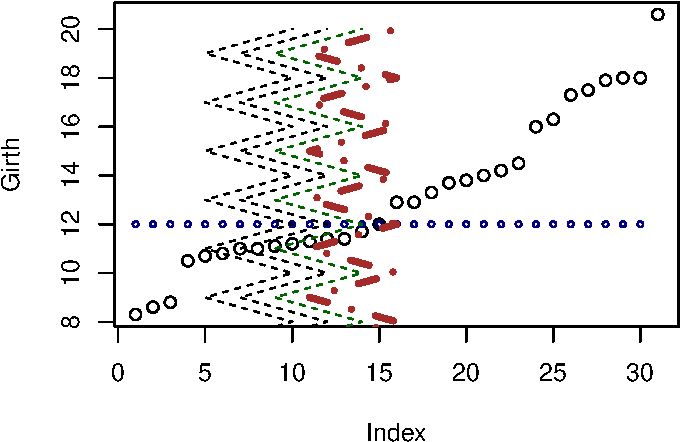
\includegraphics[width=0.5\linewidth]{Rcourse_files/figure-latex/unnamed-chunk-211-1}

We now want to estimate the (fixed) effect of the days of sleep deprivation on response time, while allowing each subject to have his/hers own effect.
Put differently, we want to estimate a \emph{random slope} for the effect of \texttt{day}.
The fixed \texttt{Days} effect can be thought of as the average slope over subjects.

\begin{Shaded}
\begin{Highlighting}[]
\NormalTok{lme}\FloatTok{.3}\NormalTok{ <-}\StringTok{ }\KeywordTok{lmer}\NormalTok{ ( Reaction }\OperatorTok{~}\StringTok{ }\NormalTok{Days }\OperatorTok{+}\StringTok{ }\NormalTok{( Days }\OperatorTok{|}\StringTok{ }\NormalTok{Subject ) , }\DataTypeTok{data=}\NormalTok{ sleepstudy )}
\end{Highlighting}
\end{Shaded}

Things to note:

\begin{itemize}
\tightlist
\item
  \texttt{\textasciitilde{}Days} specifies the fixed effect.
\item
  We used the \texttt{Days\textbar{}Subect} syntax to tell R we want to fit the model \texttt{\textasciitilde{}Days} within each subject.
\item
  Were we fitting the model for purposes of prediction only, an (almost) equivalent \texttt{lm} formulation is \texttt{lm(Reaction\textasciitilde{}Days*Subject)}.
\end{itemize}

The fixed day effect is:

\begin{Shaded}
\begin{Highlighting}[]
\KeywordTok{fixef}\NormalTok{(lme}\FloatTok{.3}\NormalTok{)}
\end{Highlighting}
\end{Shaded}

\begin{verbatim}
## (Intercept)        Days 
##   251.40510    10.46729
\end{verbatim}

The variability in the average response (intercept) and day effect is

\begin{Shaded}
\begin{Highlighting}[]
\KeywordTok{ranef}\NormalTok{(lme}\FloatTok{.3}\NormalTok{)}
\end{Highlighting}
\end{Shaded}

\begin{verbatim}
## $Subject
##     (Intercept)        Days
## 308   2.2575329   9.1992737
## 309 -40.3942719  -8.6205161
## 310 -38.9563542  -5.4495796
## 330  23.6888704  -4.8141448
## 331  22.2585409  -3.0696766
## 332   9.0387625  -0.2720535
## 333  16.8389833  -0.2233978
## 334  -7.2320462   1.0745075
## 335  -0.3326901 -10.7524799
## 337  34.8865253   8.6290208
## 349 -25.2080191   1.1730997
## 350 -13.0694180   6.6142185
## 351   4.5777099  -3.0152825
## 352  20.8614523   3.5364062
## 369   3.2750882   0.8722876
## 370 -25.6110745   4.8222518
## 371   0.8070591  -0.9881730
## 372  12.3133491   1.2842380
## 
## with conditional variances for "Subject"
\end{verbatim}

Did we really need the whole \texttt{lme} machinery to fit a within-subject linear regression and then average over subjects?
The answer is yes.
The assumptions on the distribution of random effect, namely, that they are normally distributed, allows us to pool information from one subject to another. In the words of John Tukey: ``we borrow strength over subjects''.
Is this a good thing? If the normality assumption is true, it certainly is.
If, on the other hand, you have a lot of samples per subject, and you don't need to ``borrow strength'' from one subject to another, you can simply fit within-subject linear models without the mixed-models machinery.

To demonstrate the ``strength borrowing'', here is a comparison of the lme, versus the effects of fitting a linear model to each subject separately.

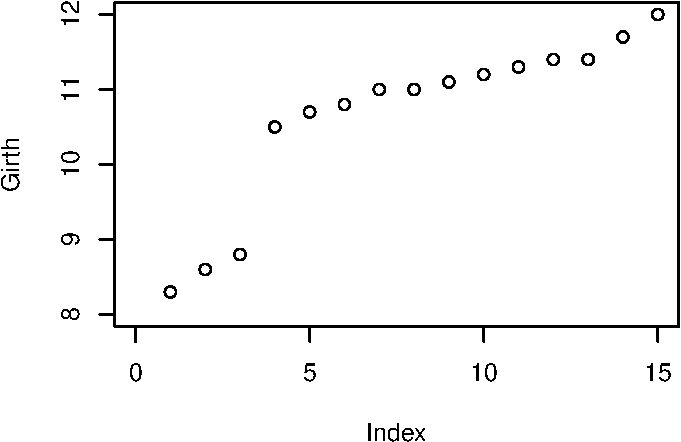
\includegraphics[width=0.5\linewidth]{Rcourse_files/figure-latex/unnamed-chunk-214-1}

Here is a comparison of the random-day effect from \texttt{lme} versus a subject-wise linear model. They are not the same.

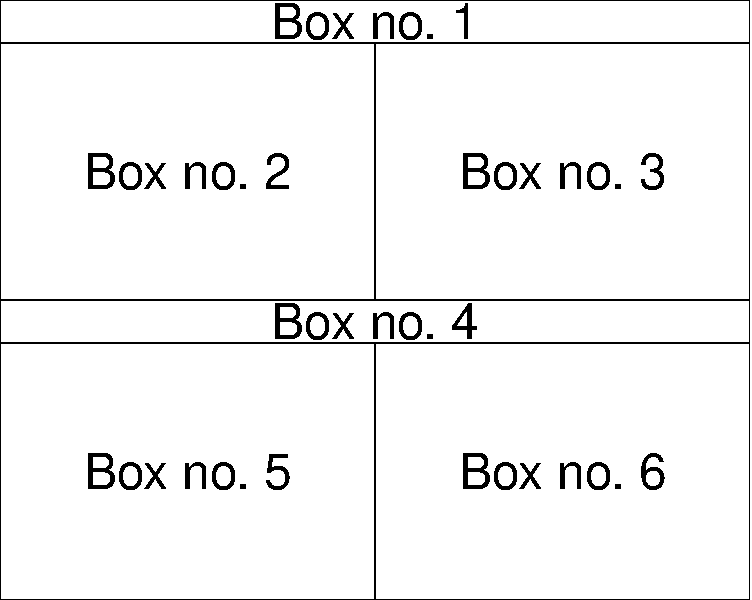
\includegraphics[width=0.5\linewidth]{Rcourse_files/figure-latex/unnamed-chunk-215-1}

\begin{Shaded}
\begin{Highlighting}[]
\KeywordTok{detach}\NormalTok{(Penicillin)}
\end{Highlighting}
\end{Shaded}

\hypertarget{serial}{%
\section{Serial Correlations}\label{serial}}

As previously stated, a hierarchical model is a very convenient way to state correlations.
The hierarchical sampling scheme will always yield correlations in blocks.
What is the correlation does not have a block structure?
Like a smooth temporal decay for time-series, or a smooth spatial decay for geospatial data?

One way to go about, is to find a dedicated package.
For instance, in the \href{https://cran.r-project.org/web/views/SpatioTemporal.html}{Spatio-Temporal Data} task view, or the \href{https://cran.r-project.org/web/views/Environmetrics.html}{Ecological and Environmental} task view.
Fans of vector-auto-regression should have a look at the \href{https://cran.r-project.org/package=vars}{vars} package.

Instead, we will show how to solve this matter using the \textbf{nlme} package.
This is because \textbf{nlme} allows to specify both a block-covariance structure using the mixed-models framework, and the smooth parametric covariances we find in temporal and spatial data.

The \texttt{nlme::Ovary} data is panel data of number of ovarian follicles in different mares (female horse), at various times.

with an AR(1) temporal correlation, alongside random-effects, we take an example from the help of \texttt{nlme::corAR1}.

\begin{Shaded}
\begin{Highlighting}[]
\KeywordTok{library}\NormalTok{(nlme)}
\KeywordTok{head}\NormalTok{(nlme}\OperatorTok{::}\NormalTok{Ovary)}
\end{Highlighting}
\end{Shaded}

\begin{verbatim}
## Grouped Data: follicles ~ Time | Mare
##   Mare        Time follicles
## 1    1 -0.13636360        20
## 2    1 -0.09090910        15
## 3    1 -0.04545455        19
## 4    1  0.00000000        16
## 5    1  0.04545455        13
## 6    1  0.09090910        10
\end{verbatim}

\begin{Shaded}
\begin{Highlighting}[]
\NormalTok{fm1Ovar.lme <-}\StringTok{ }\NormalTok{nlme}\OperatorTok{::}\KeywordTok{lme}\NormalTok{(}\DataTypeTok{fixed=}\NormalTok{follicles }\OperatorTok{~}\StringTok{ }\KeywordTok{sin}\NormalTok{(}\DecValTok{2}\OperatorTok{*}\NormalTok{pi}\OperatorTok{*}\NormalTok{Time) }\OperatorTok{+}\StringTok{ }\KeywordTok{cos}\NormalTok{(}\DecValTok{2}\OperatorTok{*}\NormalTok{pi}\OperatorTok{*}\NormalTok{Time), }
                   \DataTypeTok{data =}\NormalTok{ Ovary, }
                   \DataTypeTok{random =} \KeywordTok{pdDiag}\NormalTok{(}\OperatorTok{~}\KeywordTok{sin}\NormalTok{(}\DecValTok{2}\OperatorTok{*}\NormalTok{pi}\OperatorTok{*}\NormalTok{Time)), }
                   \DataTypeTok{correlation=}\KeywordTok{corAR1}\NormalTok{() )}
\KeywordTok{summary}\NormalTok{(fm1Ovar.lme)}
\end{Highlighting}
\end{Shaded}

\begin{verbatim}
## Linear mixed-effects model fit by REML
##  Data: Ovary 
##        AIC     BIC   logLik
##   1563.448 1589.49 -774.724
## 
## Random effects:
##  Formula: ~sin(2 * pi * Time) | Mare
##  Structure: Diagonal
##         (Intercept) sin(2 * pi * Time) Residual
## StdDev:    2.858385           1.257977 3.507053
## 
## Correlation Structure: AR(1)
##  Formula: ~1 | Mare 
##  Parameter estimate(s):
##       Phi 
## 0.5721866 
## Fixed effects: follicles ~ sin(2 * pi * Time) + cos(2 * pi * Time) 
##                        Value Std.Error  DF   t-value p-value
## (Intercept)        12.188089 0.9436602 295 12.915760  0.0000
## sin(2 * pi * Time) -2.985297 0.6055968 295 -4.929513  0.0000
## cos(2 * pi * Time) -0.877762 0.4777821 295 -1.837159  0.0672
##  Correlation: 
##                    (Intr) s(*p*T
## sin(2 * pi * Time)  0.000       
## cos(2 * pi * Time) -0.123  0.000
## 
## Standardized Within-Group Residuals:
##         Min          Q1         Med          Q3         Max 
## -2.34910093 -0.58969626 -0.04577893  0.52931186  3.37167486 
## 
## Number of Observations: 308
## Number of Groups: 11
\end{verbatim}

Things to note:

\begin{itemize}
\tightlist
\item
  The fitting is done with the \texttt{nlme::lme} function, and not \texttt{lme4::lmer} (which does not allow for non blocked covariance models).
\item
  \texttt{sin(2*pi*Time)\ +\ cos(2*pi*Time)} is a fixed effect that captures seasonality.
\item
  The temporal covariance, is specified using the \texttt{correlations=} argument.
\item
  AR(1) was assumed by calling \texttt{correlation=corAR1()}. See \texttt{nlme::corClasses} for a list of supported correlation structures.
\item
  From the summary, we see that a \texttt{Mare} random effect has also been added. Where is it specified? It is implied by the \texttt{random=} argument. Read \texttt{?lme} for further details.
\end{itemize}

We can now inspect the contrivance implied by our model's specification:

\begin{Shaded}
\begin{Highlighting}[]
\NormalTok{the.cov <-}\StringTok{ }\NormalTok{mgcv}\OperatorTok{::}\KeywordTok{extract.lme.cov}\NormalTok{(fm1Ovar.lme, }\DataTypeTok{data =}\NormalTok{ Ovary) }
\NormalTok{lattice}\OperatorTok{::}\KeywordTok{levelplot}\NormalTok{(the.cov)}
\end{Highlighting}
\end{Shaded}


\includegraphics[width=0.5\linewidth]{Rcourse_files/figure-latex/unnamed-chunk-218-1}

\hypertarget{extensions-1}{%
\section{Extensions}\label{extensions-1}}

\hypertarget{cr-se}{%
\subsection{Cluster Robust Standard Errors}\label{cr-se}}

As previously stated, random effects are nothing more than a convenient way to specify dependencies within a level of a random effect, i.e., within a group/cluster.
This is also the motivation underlying \emph{cluster robust} inference, which is immensely popular with econometricians, but less so elsewhere.
What is the difference between the two?

Mixed models framework is a bona-fide generalization of cluster robust inference.
This author thus recommends using the \textbf{lme4} and \textbf{nlme} packages for mixed models to deal with correlations within cluster.

For a longer comparison between the two approaches, see \href{https://m-clark.github.io/docs/clustered/}{Michael Clarck's guide}.

\hypertarget{linear-models-for-panel-data}{%
\subsection{Linear Models for Panel Data}\label{linear-models-for-panel-data}}

\textbf{nlme} and \textbf{lme4} will probably provide you with all the functionality you need for panel data.
If, however, you are trained as an econometrist, prefer the econometric parlance, and are not using non-linead models, then the \href{https://cran.r-project.org/package=plm}{plm} and \href{https://www.jacob-long.com/post/panelr-intro/}{panelr} packages are just for you.
In particular, it allows for cluster-robust covariance estimates, and \href{https://en.wikipedia.org/wiki/Durbin\%E2\%80\%93Wu\%E2\%80\%93Hausman_test}{Durbin--Wu--Hausman test} for random effects.
The \textbf{plm} \href{https://cran.r-project.org/web/packages/plm/vignettes/plm.pdf}{package vignette} also has a comparison to the \textbf{nlme} package.

\hypertarget{testing-hypotheses-on-correlations}{%
\subsection{Testing Hypotheses on Correlations}\label{testing-hypotheses-on-correlations}}

After working so hard to model the correlations in observation, we may want to test if it was all required.
Douglas Bates, the author of \textbf{nlme} and \textbf{lme4} wrote a famous cautionary note, \href{https://stat.ethz.ch/pipermail/r-help/2006-May/094765.html}{found here}, on hypothesis testing in mixed models.
Many practitioners, however, do not adopt Doug's view.
Many of the popular tests, particularly the ones in the econometric literature, can be found in the \textbf{plm} package (see Section 6 in the \href{https://cran.r-project.org/web/packages/plm/vignettes/plm.pdf}{package vignette}).
These include tests for poolability, Hausman test, tests for serial correlations, tests for cross-sectional dependence, and unit root tests.

\hypertarget{relation-to-other-estimators}{%
\section{Relation to Other Estimators}\label{relation-to-other-estimators}}

\hypertarget{fixed-effects-in-the-econometric-literature}{%
\subsection{Fixed Effects in the Econometric Literature}\label{fixed-effects-in-the-econometric-literature}}

Fixed effects in the statistical literature, as discussed herein, are different than those in the econometric literature.
See Section 7 of the \textbf{plm} \href{https://cran.r-project.org/web/packages/plm/vignettes/plm.pdf}{package vignette} for a comparison.

\hypertarget{relation-to-generalized-least-squares-gls}{%
\subsection{Relation to Generalized Least Squares (GLS)}\label{relation-to-generalized-least-squares-gls}}

GLS is the solution to a decorrelated least squares problem:
\[\hat{\beta}_{GLS}:=argmin_\beta\{(X'\beta-y)'\Sigma^{-1}(X'\beta-y)'\}.\]
This estimator can be viewed as a least squares estimator that accounts for correlations in the data.
It is also a maximum likelihood estimator under a Gaussian error assumption.
Viewed as the latter, then linear mixed models under a Gaussian error assumption, collapses to a GLS estimator.

\hypertarget{relation-to-conditional-gaussian-fields}{%
\subsection{Relation to Conditional Gaussian Fields}\label{relation-to-conditional-gaussian-fields}}

In the geo-spatial literature, geo-located measurements are typically assumed to be sampled from a \emph{Gaussian Random Field}.
All the models discussed in this chapter can be stated in terms of these random fields.
In the random field nomenclature, the fixed effects are known as the \emph{drift}, or the \emph{mean field}, and the covariance in errors is known as the \emph{correlation function}.
In other fields of literature the correlation function is known as a \emph{charachteristic function}, \emph{radial basis functions}, or \emph{kernel}.
Assuming stationarity, these simplify to the \emph{power spectrum} via the \emph{Wiener--Khinchin theorem}.
The predictions of such models may be found under the names of \emph{linear projection operators}, \emph{best linear unbiased prediction}, \emph{Kriging}, \emph{radial basis function interpolators}.

\hypertarget{relation-to-empirical-risk-minimization-erm}{%
\subsection{Relation to Empirical Risk Minimization (ERM)}\label{relation-to-empirical-risk-minimization-erm}}

ERM is more general than mixed-models estimation since it allows loss functions that are not the (log) likelihood.
ERM is less general than LMM, in that ERM (typically) does not account for correlations in the data.

\hypertarget{relation-to-m-estimation}{%
\subsection{Relation to M-Estimation}\label{relation-to-m-estimation}}

M-estimation is term in the statistical literature for ERM.

\hypertarget{relation-to-generalize-estimating-equations-gee}{%
\subsection{Relation to Generalize Estimating Equations (GEE)}\label{relation-to-generalize-estimating-equations-gee}}

The first order condition of the LMM problem returns a set of (non-linear) estimating equations.
In this sense, GEE can be seen as more general than LMM in that the GEE need not be the derivative of the (log) likelihood.

\hypertarget{manova}{%
\subsection{Relation to MANOVA}\label{manova}}

Multivariate analysis of variance (MANOVA) deals with the estimation of effect on \textbf{vector valued} outcomes.
Put differently: in ANOVA the response, \(y\), is univariate.
In MANOVA, the outcome is multivariate.
MANOVA is useful when there are correlations among the entries of \(y\).
Otherwise- one may simply solve many ANOVA problems, instead of a single MANOVA.

Now assume that the outcome of a MANOVA is measurements of an individual at several time periods.
The measurements are clearly correlated, so that MANOVA may be useful.
But one may also treat the subject as a random effect, with a univariate response.
We thus see that this seemingly MANOVA problem can be solved with the mixed models framework.

What MANOVA problems cannot be solved with mixed models?
There may be cases where the covariance of the multivariate outcome, \(y\), is very complicated.
If the covariance in \(y\) may not be stated using a combination of random and fixed effects, then the covariance has to be stated explicitly.
It is also possible to consider mixed-models with multivariate outcomes, i.e., a \emph{mixed MANOVA}, or \emph{hirarchial MANOVA}.
The R functions we present herein permit this.

\hypertarget{relation-to-seemingly-unrelated-equations-sur}{%
\subsection{Relation to Seemingly Unrelated Equations (SUR)}\label{relation-to-seemingly-unrelated-equations-sur}}

SUR is the econometric term for MANOVA.

\hypertarget{bibliographic-notes-6}{%
\section{Bibliographic Notes}\label{bibliographic-notes-6}}

Most of the examples in this chapter are from the documentation of the \textbf{lme4} package \citep{lme4}.
For a general and very applied treatment, see \citet{pinero2000mixed}.
As usual, a hands on view can be found in \citet{venables2013modern}, and also in an excellent blog post by \href{http://rpsychologist.com/r-guide-longitudinal-lme-lmer}{Kristoffer Magnusson}
For a more theoretical view see \citet{weiss2005modeling} or \citet{searle2009variance}.
Sometimes it is unclear if an effect is random or fixed; on the difference between the two types of inference see the classics: \citet{eisenhart1947assumptions}, \citet{kempthorne1975fixed}, and the more recent \citet{rosset2018fixed}.
For an interactive, beatiful visualization of the shrinkage introduced by mixed models, see \href{http://m-clark.github.io/posts/2019-05-14-shrinkage-in-mixed-models/}{Michael Clark's blog}.
For more on predictions in linear mixed models see \citet{robinson1991blup}, \citet{rabinowicz2018assessing}, and references therein.
See \href{https://m-clark.github.io/docs/clustered/}{Michael Clarck's} guide for various ways of dealing with correlations within groups.
For the geo-spatial view and terminology of correlated data, see \citet{christakos2000modern}, \citet{diggle1998model}, \citet{allard2013j}, and \citet{cressie2015statistics}.

\hypertarget{practice-yourself-4}{%
\section{Practice Yourself}\label{practice-yourself-4}}

\begin{enumerate}
\def\labelenumi{\arabic{enumi}.}
\item
  Computing the variance of the sample mean given dependent correlations. How does it depend on the covariance between observations? When is the sample most informative on the population mean?
\item
  Return to the \texttt{Penicillin} data set. Instead of fitting an LME model, fit an LM model with \texttt{lm}. I.e., treat all random effects as fixed.

  \begin{enumerate}
  \def\labelenumii{\alph{enumii}.}
  \tightlist
  \item
    Compare the effect estimates.
  \item
    Compare the standard errors.
  \item
    Compare the predictions of the two models.
  \end{enumerate}
\item
  {[}Very Advanced!{]} Return to the \texttt{Penicillin} data and use the \texttt{gls} function to fit a generalized linear model, equivalent to the LME model in our text.
\item
  Read about the ``oats'' dataset using \texttt{?\ MASS::oats}.Inspect the dependency of the yield (Y) in the Varieties (V) and the Nitrogen treatment (N).

  \begin{enumerate}
  \def\labelenumii{\arabic{enumii}.}
  \tightlist
  \item
    Fit a linear model, does the effect of the treatment significant? The interaction between the Varieties and Nitrogen is significant?
  \item
    An expert told you that could be a variance between the different blocks (B) which can bias the analysis. fit a LMM for the data.
  \item
    Do you think the blocks should be taken into account as ``random effect'' or ``fixed effect''?
  \end{enumerate}
\item
  Return to the temporal correlation in Section \ref{serial}, and replace the AR(1) covariance, with an ARMA covariance. Visualize the data's covariance matrix, and compare the fitted values.
\end{enumerate}

See DataCamps' \href{https://www.datacamp.com/courses/hierarchical-and-mixed-effects-models}{Hierarchical and Mixed Effects Models} for more self practice.

\hypertarget{multivariate}{%
\chapter{Multivariate Data Analysis}\label{multivariate}}

The term ``multivariate data analysis'' is so broad and so overloaded, that we start by clarifying what is discussed and what is not discussed in this chapter.
Broadly speaking, we will discuss statistical \emph{inference}, and leave more ``exploratory flavored'' matters like clustering, and visualization, to the Unsupervised Learning Chapter \ref{unsupervised}.

We start with an example.

\BeginKnitrBlock{example}
\protect\hypertarget{exm:icu}{}{\label{exm:icu} }Consider the problem of a patient monitored in the intensive care unit.
At every minute the monitor takes \(p\) physiological measurements: blood pressure, body temperature, etc.
The total number of minutes in our data is \(n\), so that in total, we have \(n \times p\) measurements, arranged in a matrix.
We also know the typical measurements for this patient when healthy: \(\mu_0\).
\EndKnitrBlock{example}

Formally, let \(y\) be single (random) measurement of a \(p\)-variate random vector.
Denote \(\mu:=E[y]\).
Here is the set of problems we will discuss, in order of their statistical difficulty.

\begin{itemize}
\item
  \textbf{Signal detection}:
  a.k.a. \emph{multivariate hypothesis testing}, i.e., testing if \(\mu\) equals \(\mu_0\) and for \(\mu_0=0\) in particular.
  In our example: ``are the current measurement different than a typical one?''
\item
  \textbf{Signal counting}:
  Counting the number of elements in \(\mu\) that differ from \(\mu_0\), and for \(\mu_0=0\) in particular.
  In our example: ``how many measurements differ than their typical values?''
\item
  \textbf{Signal identification}:
  a.k.a. \emph{multiple testing}, i.e., testing which of the elements in \(\mu\) differ from \(\mu_0\) and for \(\mu_0=0\) in particular.
  In the ANOVA literature, this is known as a \textbf{post-hoc} analysis.
  In our example: ``which measurements differ than their typical values?''
\item
  \textbf{Signal estimation}:
  Estimating the magnitudes of the departure of \(\mu\) from \(\mu_0\), and for \(\mu_0=0\) in particular.
  If estimation follows a \emph{signal detection} or \emph{signal identification} stage, this is known as a \emph{selective estimation} problem.
  In our example: ``what is the value of the measurements that differ than their typical values?''
\item
  \textbf{Multivariate Regression}:
  a.k.a. \emph{MANOVA} in statistical literature, and \emph{structured learning} in the machine learning literature.
  In our example: ``what factors affect the physiological measurements?''
\end{itemize}

\BeginKnitrBlock{example}
\protect\hypertarget{exm:brain-imaging}{}{\label{exm:brain-imaging} }Consider the problem of detecting regions of cognitive function in the brain using fMRI.
Each measurement is the activation level at each location in a brain's region.
If the region has a cognitive function, the mean activation differs than \(\mu_0=0\) when the region is evoked.
\EndKnitrBlock{example}

\BeginKnitrBlock{example}
\protect\hypertarget{exm:genetics}{}{\label{exm:genetics} }Consider the problem of detecting cancer encoding regions in the genome.
Each measurement is the vector of the genetic configuration of an individual.
A cancer encoding region will have a different (multivariate) distribution between sick and healthy.
In particular, \(\mu\) of sick will differ from \(\mu\) of healthy.
\EndKnitrBlock{example}

\BeginKnitrBlock{example}
\protect\hypertarget{exm:regression}{}{\label{exm:regression} }Consider the problem of the simplest multiple regression.
The estimated coefficient, \(\hat \beta\) are a random vector.
Regression theory tells us that its covariance is \((X'X)^{-1}\sigma^2\), and null mean of \(\beta\).
We thus see that inference on the vector of regression coefficients, is nothing more than a multivaraite inference problem.
\EndKnitrBlock{example}

\BeginKnitrBlock{remark}
\iffalse{} {Remark. } \fi{}In the above, ``signal'' is defined in terms of \(\mu\).
It is possible that the signal is not in the location, \(\mu\), but rather in the covariance, \(\Sigma\).
We do not discuss these problems here, and refer the reader to \citet{nadler2008finite}.
\EndKnitrBlock{remark}

Another possible question is: does a multivariate analysis gives us something we cannot get from a mass-univariate analysis (i.e., a multivariate analysis on each variable separately).
In Example \ref{exm:icu} we could have just performed multiple univariate tests, and sign an alarm when any of the univariate detectors was triggered.
The reason we want a multivariate detector, and not multiple univariate detectors is that it is possible that each measurement alone is borderline, but together, the signal accumulates.
In our ICU example is may mean that the pulse is borderline, the body temperature is borderline, etc. Analyzed simultaneously, it is clear that the patient is in distress.

The next figure\footnote{My thanks to Efrat Vilneski for the figure.} illustrates the idea that some bi-variate measurements may seem ordinary univariately, while very anomalous when examined bi-variately.

\BeginKnitrBlock{remark}
\iffalse{} {Remark. } \fi{}The following figure may also be used to demonstrate the difference between Euclidean Distance and Mahalanobis Distance.
\EndKnitrBlock{remark}

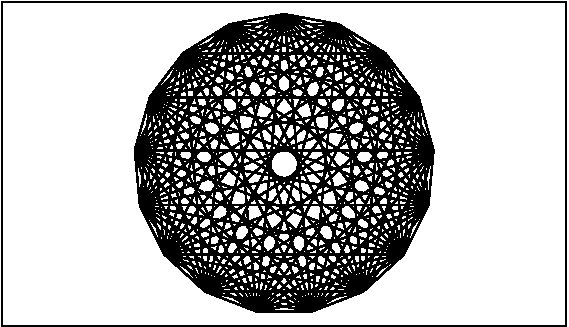
\includegraphics[width=0.5\linewidth]{Rcourse_files/figure-latex/unnamed-chunk-221-1}

\hypertarget{signal-detection}{%
\section{Signal Detection}\label{signal-detection}}

Signal detection deals with the detection of the departure of \(\mu\) from some \(\mu_0\), and especially, \(\mu_0=0\).
This problem can be thought of as the multivariate counterpart of the univariate hypothesis t-test.

\hypertarget{hotellings-t2-test}{%
\subsection{Hotelling's T2 Test}\label{hotellings-t2-test}}

The most fundamental approach to signal detection is a mere generalization of the t-test, known as \emph{Hotelling's \(T^2\) test}.

Recall the univariate t-statistic of a data vector \(x\) of length \(n\):
\begin{align}
  t^2(x):= \frac{(\bar{x}-\mu_0)^2}{Var[\bar{x}]}= (\bar{x}-\mu_0)Var[\bar{x}]^{-1}(\bar{x}-\mu_0),
  \label{eq:t-test}
\end{align}
where \(Var[\bar{x}]=S^2(x)/n\), and \(S^2(x)\) is the unbiased variance estimator \(S^2(x):=(n-1)^{-1}\sum (x_i-\bar x)^2\).

Generalizing Eq\eqref{eq:t-test} to the multivariate case:
\(\mu_0\) is a \(p\)-vector, \(\bar x\) is a \(p\)-vector, and \(Var[\bar x]\) is a \(p \times p\) matrix of the covariance between the \(p\) coordinated of \(\bar x\).
When operating with vectors, the squaring becomes a quadratic form, and the division becomes a matrix inverse.
We thus have
\begin{align}
  T^2(x):= (\bar{x}-\mu_0)' Var[\bar{x}]^{-1} (\bar{x}-\mu_0),
  \label{eq:hotelling-test}
\end{align}
which is the definition of Hotelling's \(T^2\) test statistic.
We typically denote the covariance between coordinates in \(x\) with \(\hat \Sigma(x)\), so that
\(\widehat \Sigma_{k,l}:=\widehat {Cov}[x_k,x_l]=(n-1)^{-1} \sum (x_{k,i}-\bar x_k)(x_{l,i}-\bar x_l)\).
Using the \(\Sigma\) notation, Eq.\eqref{eq:hotelling-test} becomes
\begin{align}
  T^2(x):= n (\bar{x}-\mu_0)' \hat \Sigma(x)^{-1} (\bar{x}-\mu_0),
\end{align}
which is the standard notation of Hotelling's test statistic.

For inference, we need the null distribution of Hotelling's test statistic. For this we introduce some vocabulary\footnote{This vocabulary is not standard in the literature, so when you read a text, you need to verify yourself what the author means.}:

\begin{enumerate}
\def\labelenumi{\arabic{enumi}.}
\tightlist
\item
  \textbf{Low Dimension}:
  We call a problem \emph{low dimensional} if \(n \gg p\), i.e. \(p/n \approx 0\).
  This means there are many observations per estimated parameter.
\item
  \textbf{High Dimension}:
  We call a problem \emph{high dimensional} if \(p/n \to c\), where \(c\in (0,1)\).
  This means there are more observations than parameters, but not many.
\item
  \textbf{Very High Dimension}:
  We call a problem \emph{very high dimensional} if \(p/n \to c\), where \(1<c<\infty\).
  This means there are less observations than parameter.
\end{enumerate}

Hotelling's \(T^2\) test can only be used in the low dimensional regime.
For some intuition on this statement, think of taking \(n=20\) measurements of \(p=100\) physiological variables.
We seemingly have \(20\) observations, but there are \(100\) unknown quantities in \(\mu\).
Would you trust your conclusion that \(\bar x\) is different than \(\mu_0\) based on merely \(20\) observations.

The above criticism is formalized in \citet{bai1996effect}.
For modern applications, Hotelling's \(T^2\) is not recommended, since many modern alternatives have been made available. See \citet{rosenblatt2016better} and references for a review.

\hypertarget{various-types-of-signal-to-detect}{%
\subsection{Various Types of Signal to Detect}\label{various-types-of-signal-to-detect}}

In the previous, we assumed that the signal is a departure of \(\mu\) from some \(\mu_0\).
For vactor-valued data \(y\), that is distributed \(F\), we may define ``signal'' as any departure from some \(F_0\).
This is the multivaraite counterpart of goodness-of-fit (GOF) tests.

Even when restricting ``signal'' to departures of \(\mu\) from \(\mu_0\), we may try to detect various types of signal:

\begin{enumerate}
\def\labelenumi{\arabic{enumi}.}
\tightlist
\item
  \textbf{Dense Signal}: when the departure is in all coordinates of \(\mu\).
\item
  \textbf{Sparse Signal}: when the departure is in a subset of coordinates of \(\mu\).
\end{enumerate}

A manufactoring motivation is consistent with a dense signal: if a manufacturing process has failed, we expect a change in many measurements (i.e.~coordinates of \(\mu\)).
A brain-imaging motivation is consistent with a dense signal: if a region encodes cognitive function, we expect a change in many brain locations (i.e.~coordinates of \(\mu\).)
A genetic motivation is consistent with a sparse signal: if susceptibility of disease is genetic, only a small subset of locations in the genome will encode it.

Hotelling's \(T^2\) statistic is designed for dense signal.
The following is a simple statistic designed for sparse signal.

\hypertarget{simes-test}{%
\subsection{Simes' Test}\label{simes-test}}

Hotelling's \(T^2\) statistic has currently two limitations: It is designed for dense signals, and it requires estimating the covariance, which is a very difficult problem.

An algorithm, that is sensitive to sparse signal and allows statistically valid detection under a wide range of covariances (even if we don't know the covariance) is known as \emph{Simes' Test}.
The statistic is defined vie the following algorithm:

\begin{enumerate}
\def\labelenumi{\arabic{enumi}.}
\tightlist
\item
  Compute \(p\) variable-wise p-values: \(p_1,\dots,p_j\).
\item
  Denote \(p_{(1)},\dots,p_{(j)}\) the sorted p-values.
\item
  Simes' statistic is \(p_{Simes}:=min_j\{p_{(j)} \times p/j\}\).
\item
  Reject the ``no signal'' null hypothesis at significance \(\alpha\) if \(p_{Simes}<\alpha\).
\end{enumerate}

\hypertarget{signal-detection-with-r}{%
\subsection{Signal Detection with R}\label{signal-detection-with-r}}

Let's generate some data with no signal.

\begin{Shaded}
\begin{Highlighting}[]
\KeywordTok{library}\NormalTok{(mvtnorm)}
\NormalTok{n <-}\StringTok{ }\DecValTok{100} \CommentTok{# observations}
\NormalTok{p <-}\StringTok{ }\DecValTok{18} \CommentTok{# parameter dimension}
\NormalTok{mu <-}\StringTok{ }\KeywordTok{rep}\NormalTok{(}\DecValTok{0}\NormalTok{,p) }\CommentTok{# no signal}
\NormalTok{x <-}\StringTok{ }\KeywordTok{rmvnorm}\NormalTok{(}\DataTypeTok{n =}\NormalTok{ n, }\DataTypeTok{mean =}\NormalTok{ mu)}
\KeywordTok{dim}\NormalTok{(x)}
\end{Highlighting}
\end{Shaded}

\begin{verbatim}
## [1] 100  18
\end{verbatim}

\begin{Shaded}
\begin{Highlighting}[]
\NormalTok{lattice}\OperatorTok{::}\KeywordTok{levelplot}\NormalTok{(x)}
\end{Highlighting}
\end{Shaded}

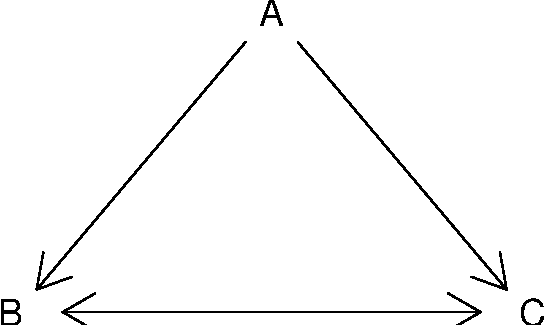
\includegraphics[width=0.5\linewidth]{Rcourse_files/figure-latex/unnamed-chunk-222-1}

Now make our own Hotelling function.

\begin{Shaded}
\begin{Highlighting}[]
\NormalTok{hotellingOneSample <-}\StringTok{ }\ControlFlowTok{function}\NormalTok{(x, }\DataTypeTok{mu0=}\KeywordTok{rep}\NormalTok{(}\DecValTok{0}\NormalTok{,}\KeywordTok{ncol}\NormalTok{(x)))\{}
\NormalTok{  n <-}\StringTok{ }\KeywordTok{nrow}\NormalTok{(x)}
\NormalTok{  p <-}\StringTok{ }\KeywordTok{ncol}\NormalTok{(x)}
  \KeywordTok{stopifnot}\NormalTok{(n }\OperatorTok{>}\StringTok{ }\DecValTok{5}\OperatorTok{*}\StringTok{ }\NormalTok{p)}
\NormalTok{  bar.x <-}\StringTok{ }\KeywordTok{colMeans}\NormalTok{(x)}
\NormalTok{  Sigma <-}\StringTok{ }\KeywordTok{var}\NormalTok{(x)}
\NormalTok{  Sigma.inv <-}\StringTok{ }\KeywordTok{solve}\NormalTok{(Sigma)}
\NormalTok{  T2 <-}\StringTok{ }\NormalTok{n }\OperatorTok{*}\StringTok{ }\NormalTok{(bar.x}\OperatorTok{-}\NormalTok{mu0) }\OperatorTok\StringTok{ }\NormalTok{Sigma.inv }\OperatorTok\StringTok{ }\NormalTok{(bar.x}\OperatorTok{-}\NormalTok{mu0)}
\NormalTok{  p.value <-}\StringTok{ }\KeywordTok{pchisq}\NormalTok{(}\DataTypeTok{q =}\NormalTok{ T2, }\DataTypeTok{df =}\NormalTok{ p, }\DataTypeTok{lower.tail =} \OtherTok{FALSE}\NormalTok{)}
  \KeywordTok{return}\NormalTok{(}\KeywordTok{list}\NormalTok{(}\DataTypeTok{statistic=}\NormalTok{T2, }\DataTypeTok{pvalue=}\NormalTok{p.value))}
\NormalTok{\}}
\KeywordTok{hotellingOneSample}\NormalTok{(x)}
\end{Highlighting}
\end{Shaded}

\begin{verbatim}
## $statistic
##          [,1]
## [1,] 17.22438
## 
## $pvalue
##           [,1]
## [1,] 0.5077323
\end{verbatim}

Things to note:

\begin{itemize}
\tightlist
\item
  \texttt{stopifnot(n\ \textgreater{}\ 5\ *\ p)} is a little verification to check that the problem is indeed low dimensional. Otherwise, the \(\chi^2\) approximation cannot be trusted.
\item
  \texttt{solve} returns a matrix inverse.
\item
  \texttt{\%*\%} is the matrix product operator (see also \texttt{crossprod()}).
\item
  A function may return only a single object, so we wrap the statistic and its p-value in a \texttt{list} object.
\end{itemize}

Just for verification, we compare our home made Hotelling's test, to the implementation in the \textbf{rrcov} package.
The statistic is clearly OK, but our \(\chi^2\) approximation of the distribution leaves room to desire.
Personally, I would never trust a Hotelling test if \(n\) is not much greater than \(p\), in which case I would use a high-dimensional adaptation (see Bibliography).

\begin{Shaded}
\begin{Highlighting}[]
\NormalTok{rrcov}\OperatorTok{::}\KeywordTok{T2.test}\NormalTok{(x)}
\end{Highlighting}
\end{Shaded}

\begin{verbatim}
## 
##  One-sample Hotelling test
## 
## data:  x
## T2 = 17.22400, F = 0.79259, df1 = 18, df2 = 82, p-value = 0.703
## alternative hypothesis: true mean vector is not equal to (0, 0, 0, 0, 0, 0, 0, 0, 0, 0, 0, 0, 0, 0, 0, 0, 0, 0)' 
## 
## sample estimates:
##                      [,1]       [,2]      [,3]       [,4]      [,5]
## mean x-vector -0.01746212 0.03776332 0.1006145 -0.2083005 0.1026982
##                      [,6]         [,7]       [,8]       [,9]       [,10]
## mean x-vector -0.05220043 -0.009497987 -0.1139856 0.02851701 -0.03089953
##                     [,11]      [,12]      [,13]      [,14]      [,15]
## mean x-vector -0.02457798 -0.1270753 0.04717076 0.01683591 0.03085023
##                   [,16]       [,17]     [,18]
## mean x-vector 0.1499485 -0.07630663 0.1004852
\end{verbatim}

Let's do the same with Simes':

\begin{Shaded}
\begin{Highlighting}[]
\NormalTok{Simes <-}\StringTok{ }\ControlFlowTok{function}\NormalTok{(x)\{}
\NormalTok{  p.vals <-}\StringTok{ }\KeywordTok{apply}\NormalTok{(x, }\DecValTok{2}\NormalTok{, }\ControlFlowTok{function}\NormalTok{(z) }\KeywordTok{t.test}\NormalTok{(z)}\OperatorTok{$}\NormalTok{p.value) }\CommentTok{# Compute variable-wise pvalues}
\NormalTok{  p <-}\StringTok{ }\KeywordTok{ncol}\NormalTok{(x)}
\NormalTok{  p.Simes <-}\StringTok{ }\NormalTok{p }\OperatorTok{*}\StringTok{ }\KeywordTok{min}\NormalTok{(}\KeywordTok{sort}\NormalTok{(p.vals)}\OperatorTok{/}\KeywordTok{seq_along}\NormalTok{(p.vals)) }\CommentTok{# Compute the Simes statistic}
  \KeywordTok{return}\NormalTok{(}\KeywordTok{c}\NormalTok{(}\DataTypeTok{pvalue=}\NormalTok{p.Simes))}
\NormalTok{\}}
\KeywordTok{Simes}\NormalTok{(x)}
\end{Highlighting}
\end{Shaded}

\begin{verbatim}
##    pvalue 
## 0.6398998
\end{verbatim}

And now we verify that both tests can indeed detect signal when present. Are p-values small enough to reject the ``no signal'' null hypothesis?

\begin{Shaded}
\begin{Highlighting}[]
\NormalTok{mu <-}\StringTok{ }\KeywordTok{rep}\NormalTok{(}\DataTypeTok{x =} \DecValTok{10}\OperatorTok{/}\NormalTok{p,}\DataTypeTok{times=}\NormalTok{p) }\CommentTok{# inject signal}
\NormalTok{x <-}\StringTok{ }\KeywordTok{rmvnorm}\NormalTok{(}\DataTypeTok{n =}\NormalTok{ n, }\DataTypeTok{mean =}\NormalTok{ mu)}
\KeywordTok{hotellingOneSample}\NormalTok{(x)}
\end{Highlighting}
\end{Shaded}

\begin{verbatim}
## $statistic
##          [,1]
## [1,] 686.8046
## 
## $pvalue
##               [,1]
## [1,] 3.575926e-134
\end{verbatim}

\begin{Shaded}
\begin{Highlighting}[]
\KeywordTok{Simes}\NormalTok{(x)}
\end{Highlighting}
\end{Shaded}

\begin{verbatim}
##       pvalue 
## 2.765312e-10
\end{verbatim}

\ldots{} yes. All p-values are very small, so that all statistics can detect the non-null distribution.

\hypertarget{signal-counting}{%
\section{Signal Counting}\label{signal-counting}}

There are many ways to approach the \emph{signal counting} problem.
For the purposes of this book, however, we will not discuss them directly, and solve the signal counting problem as a signal identification problem: if we know \textbf{where} \(\mu\) departs from \(\mu_0\), we only need to count coordinates to solve the signal counting problem.

\BeginKnitrBlock{remark}
\iffalse{} {Remark. } \fi{}In the sparsity or multiple-testing literature, what we call ``signal counting'' is known as ``adapting to sparsit'', or ``adaptivity''.
\EndKnitrBlock{remark}

\hypertarget{identification}{%
\section{Signal Identification}\label{identification}}

The problem of \emph{signal identification} is also known as \emph{selective testing}, or more commonly as \emph{multiple testing}.

In the ANOVA literature, an identification stage will typically follow a detection stage.
These are known as the \emph{omnibus F test}, and \emph{post-hoc} tests, respectively.
In the multiple testing literature there will typically be no preliminary detection stage. It is typically assumed that signal is present, and the only question is ``where?''

The first question when approaching a multiple testing problem is ``what is an error''?
Is an error declaring a coordinate in \(\mu\) to be different than \(\mu_0\) when it is actually not?
Is an error an overly high proportion of falsely identified coordinates?
The former is known as the \emph{family wise error rate} (FWER), and the latter as the \emph{false discovery rate} (FDR).

\BeginKnitrBlock{remark}
\iffalse{} {Remark. } \fi{}These types of errors have many names in many communities.
See the Wikipedia entry on \href{https://en.wikipedia.org/wiki/Receiver_operating_characteristic}{ROC} for a table of the (endless) possible error measures.
\EndKnitrBlock{remark}

\hypertarget{signal-identification-in-r}{%
\subsection{Signal Identification in R}\label{signal-identification-in-r}}

One (of many) ways to do signal identification involves the \texttt{stats::p.adjust} function.
The function takes as inputs a \(p\)-vector of the variable-wise \textbf{p-values}.
Why do we start with variable-wise p-values, and not the full data set?

\begin{enumerate}
\def\labelenumi{\alph{enumi}.}
\tightlist
\item
  Because we want to make inference variable-wise, so it is natural to start with variable-wise statistics.
\item
  Because we want to avoid dealing with covariances if possible. Computing variable-wise p-values does not require estimating covariances.
\item
  So that the identification problem is decoupled from the variable-wise inference problem, and may be applied much more generally than in the setup we presented.
\end{enumerate}

We start be generating some high-dimensional multivariate data and computing the coordinate-wise (i.e.~hypothesis-wise) p-value.

\begin{Shaded}
\begin{Highlighting}[]
\KeywordTok{library}\NormalTok{(mvtnorm)}
\NormalTok{n <-}\StringTok{ }\FloatTok{1e1}
\NormalTok{p <-}\StringTok{ }\FloatTok{1e2}
\NormalTok{mu <-}\StringTok{ }\KeywordTok{rep}\NormalTok{(}\DecValTok{0}\NormalTok{,p)}
\NormalTok{x <-}\StringTok{ }\KeywordTok{rmvnorm}\NormalTok{(}\DataTypeTok{n =}\NormalTok{ n, }\DataTypeTok{mean =}\NormalTok{ mu)}
\KeywordTok{dim}\NormalTok{(x)}
\end{Highlighting}
\end{Shaded}

\begin{verbatim}
## [1]  10 100
\end{verbatim}

\begin{Shaded}
\begin{Highlighting}[]
\NormalTok{lattice}\OperatorTok{::}\KeywordTok{levelplot}\NormalTok{(x)}
\end{Highlighting}
\end{Shaded}

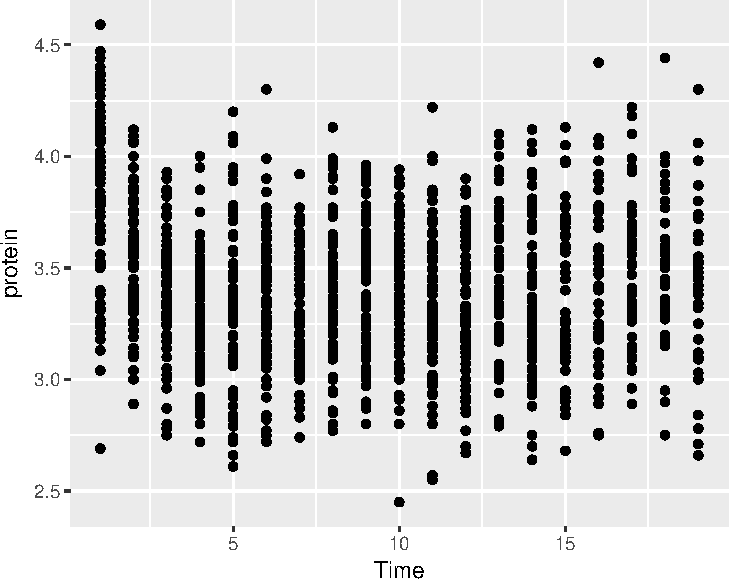
\includegraphics[width=0.5\linewidth]{Rcourse_files/figure-latex/unnamed-chunk-229-1}

We now compute the pvalues of each coordinate.
We use a coordinate-wise t-test.
Why a t-test? Because for the purpose of demonstration we want a simple test. In reality, you may use any test that returns valid p-values.

\begin{Shaded}
\begin{Highlighting}[]
\NormalTok{t.pval <-}\StringTok{ }\ControlFlowTok{function}\NormalTok{(y) }\KeywordTok{t.test}\NormalTok{(y)}\OperatorTok{$}\NormalTok{p.value}
\NormalTok{p.values <-}\StringTok{ }\KeywordTok{apply}\NormalTok{(}\DataTypeTok{X =}\NormalTok{ x, }\DataTypeTok{MARGIN =} \DecValTok{2}\NormalTok{, }\DataTypeTok{FUN =}\NormalTok{ t.pval) }
\KeywordTok{plot}\NormalTok{(p.values, }\DataTypeTok{type=}\StringTok{'h'}\NormalTok{)}
\end{Highlighting}
\end{Shaded}

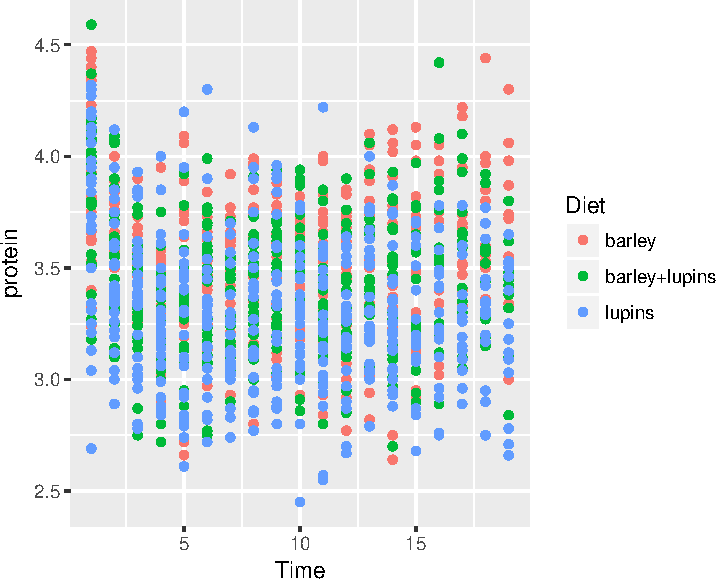
\includegraphics[width=0.5\linewidth]{Rcourse_files/figure-latex/unnamed-chunk-230-1}

Things to note:

\begin{itemize}
\tightlist
\item
  \texttt{t.pval} is a function that merely returns the p-value of a t.test.
\item
  We used the \texttt{apply} function to apply the same function to each column of \texttt{x}.
\item
  \texttt{MARGIN=2} tells \texttt{apply} to compute over columns and not rows.
\item
  The output, \texttt{p.values}, is a vector of 100 p-values.
\end{itemize}

We are now ready to do the identification, i.e., find which coordinate of \(\mu\) is different than \(\mu_0=0\).
The workflow for identification has the same structure, regardless of the desired error guarantees:

\begin{enumerate}
\def\labelenumi{\arabic{enumi}.}
\tightlist
\item
  Compute an \texttt{adjusted\ p-value}.
\item
  Compare the adjusted p-value to the desired error level.
\end{enumerate}

If we want \(FWER \leq 0.05\), meaning that we allow a \(5\%\) probability of making any mistake, we will use the \texttt{method="holm"} argument of \texttt{p.adjust}.

\begin{Shaded}
\begin{Highlighting}[]
\NormalTok{alpha <-}\StringTok{ }\FloatTok{0.05}
\NormalTok{p.values.holm <-}\StringTok{ }\KeywordTok{p.adjust}\NormalTok{(p.values, }\DataTypeTok{method =} \StringTok{'holm'}\NormalTok{ )}
\KeywordTok{which}\NormalTok{(p.values.holm }\OperatorTok{<}\StringTok{ }\NormalTok{alpha)}
\end{Highlighting}
\end{Shaded}

\begin{verbatim}
## integer(0)
\end{verbatim}

If we want \(FDR \leq 0.05\), meaning that we allow the proportion of false discoveries to be no larger than \(5\%\), we use the \texttt{method="BH"} argument of \texttt{p.adjust}.

\begin{Shaded}
\begin{Highlighting}[]
\NormalTok{alpha <-}\StringTok{ }\FloatTok{0.05}
\NormalTok{p.values.BH <-}\StringTok{ }\KeywordTok{p.adjust}\NormalTok{(p.values, }\DataTypeTok{method =} \StringTok{'BH'}\NormalTok{ )}
\KeywordTok{which}\NormalTok{(p.values.BH }\OperatorTok{<}\StringTok{ }\NormalTok{alpha)}
\end{Highlighting}
\end{Shaded}

\begin{verbatim}
## integer(0)
\end{verbatim}

We now inject some strong signal in \(\mu\) just to see that the process works.
We will artificially inject signal in the first 10 coordinates.

\begin{Shaded}
\begin{Highlighting}[]
\NormalTok{mu[}\DecValTok{1}\OperatorTok{:}\DecValTok{10}\NormalTok{] <-}\StringTok{ }\DecValTok{2} \CommentTok{# inject signal in first 10 variables}
\NormalTok{x <-}\StringTok{ }\KeywordTok{rmvnorm}\NormalTok{(}\DataTypeTok{n =}\NormalTok{ n, }\DataTypeTok{mean =}\NormalTok{ mu) }\CommentTok{# generate data}
\NormalTok{p.values <-}\StringTok{ }\KeywordTok{apply}\NormalTok{(}\DataTypeTok{X =}\NormalTok{ x, }\DataTypeTok{MARGIN =} \DecValTok{2}\NormalTok{, }\DataTypeTok{FUN =}\NormalTok{ t.pval) }
\NormalTok{p.values.BH <-}\StringTok{ }\KeywordTok{p.adjust}\NormalTok{(p.values, }\DataTypeTok{method =} \StringTok{'BH'}\NormalTok{ )}
\KeywordTok{which}\NormalTok{(p.values.BH }\OperatorTok{<}\StringTok{ }\NormalTok{alpha)}
\end{Highlighting}
\end{Shaded}

\begin{verbatim}
##  [1]  1  2  3  4  5  6  7  9 10 55
\end{verbatim}

Indeed- we are now able to detect that the first coordinates carry signal, because their respective coordinate-wise null hypotheses have been rejected.

\hypertarget{signal-estimation}{%
\section{Signal Estimation (*)}\label{signal-estimation}}

The estimation of the elements of \(\mu\) is a seemingly straightforward task.
This is not the case, however, if we estimate only the elements that were selected because they were significant (or any other data-dependent criterion).
Clearly, estimating only significant entries will introduce a bias in the estimation.
In the statistical literature, this is known as \emph{selection bias}.
Selection bias also occurs when you perform inference on regression coefficients after some model selection, say, with a lasso, or a forward search\footnote{You might find this shocking, but it does mean that you cannot trust the \texttt{summary} table of a model that was selected from a multitude of models.}.

Selective inference is a complicated and active research topic so we will not offer any off-the-shelf solution to the matter.
The curious reader is invited to read \citet{rosenblatt2014selective}, \citet{javanmard2014confidence}, or \href{http://www.stat.berkeley.edu/~wfithian/}{Will Fithian's} PhD thesis \citep{fithian2015topics} for more on the topic.

\hypertarget{bibliographic-notes-7}{%
\section{Bibliographic Notes}\label{bibliographic-notes-7}}

For a general introduction to multivariate data analysis see \citet{anderson2004introduction}.
For an R oriented introduction, see \citet{everitt2011introduction}.
For more on the difficulties with high dimensional problems, see \citet{bai1996effect}.
For some cutting edge solutions for testing in high-dimension, see \citet{rosenblatt2016better} and references therein.
Simes' test is not very well known. It is introduced in \citet{simes1986improved}, and proven to control the type I error of detection under a PRDS type of dependence in \citet{benjamini2001control}.
For more on multiple testing, and signal identification, see \citet{efron2012large}.
For more on the choice of your error rate see \citet{rosenblatt2013practitioner}.
For an excellent review on graphical models see \citet{kalisch2014causal}.
Everything you need on graphical models, Bayesian belief networks, and structure learning in R, is collected in the \href{https://cran.r-project.org/web/views/gR.html}{Task View}.

\hypertarget{practice-yourself-5}{%
\section{Practice Yourself}\label{practice-yourself-5}}

\begin{enumerate}
\def\labelenumi{\arabic{enumi}.}
\item
  Generate multivariate data with:

\begin{Shaded}
\begin{Highlighting}[]
\KeywordTok{set.seed}\NormalTok{(}\DecValTok{3}\NormalTok{)}
\NormalTok{mean<-}\KeywordTok{rexp}\NormalTok{(}\DecValTok{50}\NormalTok{,}\DecValTok{6}\NormalTok{)}
\NormalTok{multi<-}\StringTok{  }\KeywordTok{rmvnorm}\NormalTok{(}\DataTypeTok{n =} \DecValTok{100}\NormalTok{, }\DataTypeTok{mean =}\NormalTok{ mean) }
\end{Highlighting}
\end{Shaded}

  \begin{enumerate}
  \def\labelenumii{\alph{enumii}.}
  \tightlist
  \item
    Use Hotelling's test to determine if \(\mu\) equals \(\mu_0=0\). Can you detect the signal?
  \item
    Perform t.test on each variable and extract the p-value. Try to identify visually the variables which depart from \(\mu_0\).
  \item
    Use \texttt{p.adjust} to identify in which variables there are any departures from \(\mu_0=0\). Allow 5\% probability of making any false identification.
  \item
    Use \texttt{p.adjust} to identify in which variables there are any departures from \(\mu_0=0\). Allow a 5\% proportion of errors within identifications.
  \end{enumerate}
\item
  Generate multivariate data from two groups: \texttt{rmvnorm(n\ =\ 100,\ mean\ =\ rep(0,10))} for the first, and \texttt{rmvnorm(n\ =\ 100,\ mean\ =\ rep(0.1,10))} for the second.

  \begin{enumerate}
  \def\labelenumii{\alph{enumii}.}
  \tightlist
  \item
    Do we agree the groups differ?
  \item
    Implement the two-group Hotelling test described in Wikipedia: (\url{https://en.wikipedia.org/wiki/Hotelling\%27s_T-squared_distribution\#Two-sample_statistic}).
  \item
    Verify that you are able to detect that the groups differ.
  \item
    Perform a two-group t-test on each coordinate. On which coordinates can you detect signal while controlling the FWER? On which while controlling the FDR? Use \texttt{p.adjust}.
  \end{enumerate}
\item
  Return to the previous problem, but set \texttt{n=9}. Verify that you cannot compute your Hotelling statistic.
\end{enumerate}

\hypertarget{supervised}{%
\chapter{Supervised Learning}\label{supervised}}

Machine learning is very similar to statistics, but it is certainly not the same.
As the name suggests, in machine learning we want machines to learn.
This means that we want to replace hard-coded expert algorithm, with data-driven self-learned algorithm.

There are many learning setups, that depend on what information is available to the machine.
The most common setup, discussed in this chapter, is \emph{supervised learning}.
The name takes from the fact that by giving the machine data samples with known inputs (a.k.a. features) and desired outputs (a.k.a. labels), the human is effectively supervising the learning.
If we think of the inputs as predictors, and outcomes as predicted, it is no wonder that supervised learning is very similar to statistical prediction.
When asked ``are these the same?'' I like to give the example of internet fraud.
If you take a sample of fraud ``attacks'', a statistical formulation of the problem is highly unlikely.
This is because fraud events are not randomly drawn from some distribution, but rather, arrive from an adversary learning the defenses and adapting to it.
This instance of supervised learning is more similar to game theory than statistics.

Other types of machine learning problems include \citep{sammut2011encyclopedia}:

\begin{itemize}
\item
  \textbf{Unsupervised Learning}:
  Where we merely analyze the inputs/features, but no desirable outcome is available to the learning machine.
  See Chapter \ref{unsupervised}.
\item
  \textbf{Semi Supervised Learning}:
  Where only part of the samples are labeled.
  A.k.a. \emph{co-training}, \emph{learning from labeled and unlabeled data}, \emph{transductive learning}.
\item
  \textbf{Active Learning}:
  Where the machine is allowed to query the user for labels. Very similar to \emph{adaptive design of experiments}.
\item
  \textbf{Learning on a Budget}:
  A version of active learning where querying for labels induces variable costs.
\item
  \textbf{Weak Learning}:
  A version of supervised learning where the labels are given not by an expert, but rather by some heuristic rule.
  Example: mass-labeling cyber attacks by a rule based software, instead of a manual inspection.
\item
  \textbf{Reinforcement Learning}:\\
  Similar to active learning, in that the machine may query for labels.
  Different from active learning, in that the machine does not receive labels, but \emph{rewards}.
\item
  \textbf{Structure Learning}:
  An instance of supervised learning where we predict objects with structure such as dependent vectors, graphs, images, tensors, etc.
\item
  \textbf{Online Learning}:
  An instance of supervised learning, where we need to make predictions where data inputs as a stream.
\item
  \textbf{Transduction}:
  An instance of supervised learning where we need to make predictions for a new set of predictors, but which are known at the time of learning.
  Can be thought of as semi-supervised \emph{extrapolation}.
\item
  \textbf{Covariate shift}:
  An instance of supervised learning where we need to make predictions for a set of predictors that ha a different distribution than the data generating source.
\item
  \textbf{Targeted Learning}:
  A form of supervised learning, designed at causal inference for decision making.
\item
  \textbf{Co-training}:
  An instance of supervised learning where we solve several problems, and exploit some assumed relation between the problems.
\item
  \textbf{Manifold learning}: An instance of unsupervised learning, where the goal is to reduce the dimension of the data by embedding it into a lower dimensional manifold.
  A.k.a. \emph{support estimation}.
\item
  \textbf{Similarity Learning}: Where we try to learn how to measure similarity between objects (like faces, texts, images, etc.).
\item
  \textbf{Metric Learning}: Like \emph{similarity learning}, only that the similarity has to obey the definition of a \emph{metric}.
\item
  \textbf{Learning to learn}:
  Deals with the carriage of ``experience'' from one learning problem to another.
  A.k.a. \emph{cummulative learning}, \emph{knowledge transfer}, and \emph{meta learning}.
\end{itemize}

\hypertarget{problem-setup-3}{%
\section{Problem Setup}\label{problem-setup-3}}

We now present the \emph{empirical risk minimization} (ERM) approach to supervised learning, a.k.a. \emph{M-estimation} in the statistical literature.

\BeginKnitrBlock{remark}
\iffalse{} {Remark. } \fi{}We do not discuss purely algorithmic approaches such as K-nearest neighbour and \emph{kernel smoothing} due to space constraints.
For a broader review of supervised learning, see the Bibliographic Notes.
\EndKnitrBlock{remark}

\BeginKnitrBlock{example}[Rental Prices]
\protect\hypertarget{exm:rental-prices}{}{\label{exm:rental-prices} \iffalse (Rental Prices) \fi{} }Consider the problem of predicting if a mail is spam or not based on its attributes: length, number of exclamation marks, number of recipients, etc.
\EndKnitrBlock{example}

Given \(n\) samples with inputs \(x\) from some space \(\mathcal{X}\) and desired outcome, \(y\), from some space \(\mathcal{Y}\).
In our example, \(y\) is the spam/no-spam label, and \(x\) is a vector of the mail's attributes.
Samples, \((x,y)\) have some distribution we denote \(P\).
We want to learn a function that maps inputs to outputs, i.e., that classifies to spam given. This function is called a \emph{hypothesis}, or \emph{predictor}, denoted \(f\), that belongs to a hypothesis class \(\mathcal{F}\) such that \(f:\mathcal{X} \to \mathcal{Y}\).
We also choose some other function that fines us for erroneous prediction.
This function is called the \emph{loss}, and we denote it by \(l:\mathcal{Y}\times \mathcal{Y} \to \mathbb{R}^+\).

\BeginKnitrBlock{remark}
\iffalse{} {Remark. } \fi{}The \emph{hypothesis} in machine learning is only vaguely related the \emph{hypothesis} in statistical testing, which is quite confusing.
\EndKnitrBlock{remark}

\BeginKnitrBlock{remark}
\iffalse{} {Remark. } \fi{}The \emph{hypothesis} in machine learning is not a bona-fide \emph{statistical model} since we don't assume it is the data generating process, but rather some function which we choose for its good predictive performance.
\EndKnitrBlock{remark}

The fundamental task in supervised (statistical) learning is to recover a hypothesis that minimizes the average loss in the sample, and not in the population.
This is know as the \emph{risk minimization problem}.

\BeginKnitrBlock{definition}[Risk Function]
\protect\hypertarget{def:unnamed-chunk-236}{}{\label{def:unnamed-chunk-236} \iffalse (Risk Function) \fi{} }The \emph{risk function}, a.k.a. \emph{generalization error}, or \emph{test error}, is the population average loss of a predictor \(f\):
\begin{align}
  R(f):=\mathbb{E}_P[l(f(x),y)].
\end{align}
\EndKnitrBlock{definition}

The best predictor, is the risk minimizer:
\begin{align}
  f^* := argmin_f \{R(f)\}.
  \label{eq:risk}  
\end{align}

Another fundamental problem is that we do not know the distribution of all possible inputs and outputs, \(P\).
We typically only have a sample of \((x_i,y_i), i=1,\dots,n\).
We thus state the \emph{empirical} counterpart of \eqref{eq:risk}, which consists of minimizing the average loss.
This is known as the \emph{empirical risk miminization} problem (ERM).

\BeginKnitrBlock{definition}[Empirical Risk]
\protect\hypertarget{def:unnamed-chunk-237}{}{\label{def:unnamed-chunk-237} \iffalse (Empirical Risk) \fi{} }The \emph{empirical risk function}, a.k.a. \emph{in-sample error}, or \emph{train error}, is the sample average loss of a predictor \(f\):
\begin{align}
  R_n(f):= 1/n \sum_i l(f(x_i),y_i).
\end{align}
\EndKnitrBlock{definition}

A good candidate proxy for \(f^*\) is its empirical counterpart, \(\hat f\), known as the \emph{empirical risk minimizer}:
\begin{align}
  \hat f := argmin_f \{ R_n(f) \}.
  \label{eq:erm}  
\end{align}

To make things more explicit:

\begin{itemize}
\tightlist
\item
  \(f\) may be a linear function of the attributes, so that it may be indexed simply with its coefficient vector \(\beta\).
\item
  \(l\) may be a squared error loss: \(l(f(x),y):=(f(x)-y)^2\).
\end{itemize}

Under these conditions, the best predictor \(f^* \in \mathcal{F}\) from problem \eqref{eq:risk} is to
\begin{align}
  f^* := argmin_\beta \{ \mathbb{E}_{P(x,y)}[(x'\beta-y)^2] \}.
\end{align}

When using a linear hypothesis with squared loss, we see that the empirical risk minimization problem collapses to an ordinary least-squares problem:
\begin{align}
  \hat f := argmin_\beta \{1/n \sum_i (x_i'\beta - y_i)^2 \}.
\end{align}

When data samples are assumingly independent, then maximum likelihood estimation is also an instance of ERM, when using the (negative) log likelihood as the loss function.

If we don't assume any structure on the hypothesis, \(f\), then \(\hat f\) from \eqref{eq:erm} will interpolate the data, and \(\hat f\) will be a very bad predictor.
We say, it will \emph{overfit} the observed data, and will have bad performance on new data.

We have several ways to avoid overfitting:

\begin{enumerate}
\def\labelenumi{\arabic{enumi}.}
\tightlist
\item
  Restrict the hypothesis class \(\mathcal{F}\) (such as linear functions).
\item
  Penalize for the complexity of \(f\). The penalty denoted by \(\Vert f \Vert\).
\item
  Unbiased risk estimation:
  \(R_n(f)\) is not an unbiased estimator of \(R(f)\).
  Why? Think of estimating the mean with the sample minimum\ldots{}
  Because \(R_n(f)\) is downward biased, we may add some correction term, or compute \(R_n(f)\) on different data than the one used to recover \(\hat f\).
\end{enumerate}

Almost all ERM algorithms consist of some combination of all the three methods above.

\hypertarget{common-hypothesis-classes}{%
\subsection{Common Hypothesis Classes}\label{common-hypothesis-classes}}

Some common hypothesis classes, \(\mathcal{F}\), with restricted complexity, are:

\begin{enumerate}
\def\labelenumi{\arabic{enumi}.}
\item
  \textbf{Linear hypotheses}: such as linear models, GLMs, and (linear) support vector machines (SVM).
\item
  \textbf{Neural networks}: a.k.a. \emph{feed-forward} neural nets, \emph{artificial} neural nets, and the celebrated class of \emph{deep} neural nets.
\item
  \textbf{Tree}: a.k.a. \emph{decision rules}, is a class of hypotheses which can be stated as ``if-then'' rules.
\item
  \textbf{Reproducing Kernel Hilbert Space}: a.k.a. RKHS, is a subset of ``the space of all functions\footnote{It is even a subset of the Hilbert space, itself a subset of the space of all functions.}'' that is both large enough to capture very complicated relations, but small enough so that it is less prone to overfitting, and also surprisingly simple to compute with.
\end{enumerate}

\hypertarget{common-complexity-penalties}{%
\subsection{Common Complexity Penalties}\label{common-complexity-penalties}}

The most common complexity penalty applies to classes that have a finite dimensional parametric representation, such as the class of linear predictors, parametrized via its coefficients \(\beta\).
In such classes we may penalize for the norm of the parameters.
Common penalties include:

\begin{enumerate}
\def\labelenumi{\arabic{enumi}.}
\tightlist
\item
  \textbf{Ridge penalty}: penalizing the \(l_2\) norm of the parameter. I.e. \(\Vert f \Vert=\Vert \beta \Vert_2^2=\sum_j \beta_j^2\).
\item
  \textbf{LASSO penalty}: penalizing the \(l_1\) norm of the parameter. I.e., \(\Vert f \Vert=\Vert \beta \Vert_1=\sum_j |\beta_j|\). Also known as \textbf{Basis Pursuit}, in signal processing.
\item
  \textbf{Elastic net}: a combination of the lasso and ridge penalty. I.e. ,\(\Vert f \Vert= \alpha \Vert \beta \Vert_2^2 + (1-\alpha) \Vert \beta \Vert_1\).
\item
  \textbf{Function Norms}: If the hypothesis class \(\mathcal{F}\) does not admit a finite dimensional representation, the penalty is no longer a function of the parameters of the function. We may, however, penalize not the parametric representation of the function, but rather the function itself \(\Vert f \Vert=\sqrt{\int f(t)^2 dt}\).
\end{enumerate}

\hypertarget{unbiased-risk-estimation}{%
\subsection{Unbiased Risk Estimation}\label{unbiased-risk-estimation}}

The fundamental problem of overfitting, is that the empirical risk, \(R_n(\hat f)\), is downward biased to the population risk, \(R(\hat f)\).
We can remove this bias in two ways:
(a) purely algorithmic \emph{resampling} approaches, and (b) theory driven estimators.

\begin{enumerate}
\def\labelenumi{\arabic{enumi}.}
\item
  \textbf{Train-Validate-Test}:
  The simplest form of algorithmic validation is to split the data.
  A \emph{train} set to train/estimate/learn \(\hat f\).
  A \emph{validation} set to compute the out-of-sample expected loss, \(R(\hat f)\), and pick the best performing predictor.
  A \emph{test} sample to compute the out-of-sample performance of the selected hypothesis.
  This is a very simple approach, but it is very ``data inefficient'', thus motivating the next method.
\item
  \textbf{V-Fold Cross Validation}:
  By far the most popular algorithmic unbiased risk estimator; in \emph{V-fold CV} we ``fold'' the data into \(V\) non-overlapping sets.
  For each of the \(V\) sets, we learn \(\hat f\) with the non-selected fold, and assess \(R(\hat f)\)) on the selected fold.
  We then aggregate results over the \(V\) folds, typically by averaging.
\item
  \textbf{AIC}:
  Akaike's information criterion (AIC) is a theory driven correction of the empirical risk, so that it is unbiased to the true risk.
  It is appropriate when using the likelihood loss.
\item
  \textbf{Cp}:
  Mallow's Cp is an instance of AIC for likelihood loss under normal noise.
\end{enumerate}

Other theory driven unbiased risk estimators include the \emph{Bayesian Information Criterion} (BIC, aka SBC, aka SBIC), the \emph{Minimum Description Length} (MDL), \emph{Vapnic's Structural Risk Minimization} (SRM), the \emph{Deviance Information Criterion} (DIC), and the \emph{Hannan-Quinn Information Criterion} (HQC).

Other resampling based unbiased risk estimators include resampling \textbf{without replacement} algorithms like \emph{delete-d cross validation} with its many variations, and \textbf{resampling with replacement}, like the \emph{bootstrap}, with its many variations.

\hypertarget{collecting-the-pieces}{%
\subsection{Collecting the Pieces}\label{collecting-the-pieces}}

An ERM problem with regularization will look like
\begin{align}
  \hat f := argmin_{f \in \mathcal{F}} \{ R_n(f)  + \lambda \Vert f \Vert \}.
  \label{eq:erm-regularized}  
\end{align}

Collecting ideas from the above sections, a typical supervised learning pipeline will include: choosing the hypothesis class, choosing the penalty function and level, unbiased risk estimator.
We emphasize that choosing the penalty function, \(\Vert f \Vert\) is not enough, and we need to choose how ``hard'' to apply it.
This if known as the \emph{regularization level}, denoted by \(\lambda\) in Eq.\eqref{eq:erm-regularized}.

Examples of such combos include:

\begin{enumerate}
\def\labelenumi{\arabic{enumi}.}
\tightlist
\item
  Linear regression, no penalty, train-validate test.
\item
  Linear regression, no penalty, AIC.
\item
  Linear regression, \(l_2\) penalty, V-fold CV. This combo is typically known as \emph{ridge regression}.
\item
  Linear regression, \(l_1\) penalty, V-fold CV. This combo is typically known as \emph{LASSO regression}.
\item
  Linear regression, \(l_1\) and \(l_2\) penalty, V-fold CV. This combo is typically known as \emph{elastic net regression}.
\item
  Logistic regression, \(l_2\) penalty, V-fold CV.
\item
  SVM classification, \(l_2\) penalty, V-fold CV.
\item
  Deep network, no penalty, V-fold CV.
\item
  Unrestricted, \(\Vert \partial^2 f \Vert_2\), V-fold CV. This combo is typically known as a \emph{smoothing spline}.
\end{enumerate}

For fans of statistical hypothesis testing we will also emphasize:
Testing and prediction are related, but are not the same:

\begin{itemize}
\tightlist
\item
  In the current chapter, we do not claim our models, \(f\), are generative. I.e., we do not claim that there is some causal relation between \(x\) and \(y\). We only claim that \(x\) predicts \(y\).
\item
  It is possible that we will want to ignore a significant predictor, and add a non-significant one \citep{foster2004variable}.
\item
  Some authors will use hypothesis testing as an initial screening for candidate predictors.
  This is a useful heuristic, but that is all it is-- a heuristic. It may also fail miserably if predictors are linearly dependent (a.k.a. multicollinear).
\end{itemize}

\hypertarget{supervised-learning-in-r}{%
\section{Supervised Learning in R}\label{supervised-learning-in-r}}

At this point, we have a rich enough language to do supervised learning with R.

In these examples, I will use two data sets from the \textbf{ElemStatLearn} package, that accompanies the seminal book by \citet{friedman2001elements}.
I use the \texttt{spam} data for categorical predictions, and \texttt{prostate} for continuous predictions.
In \texttt{spam} we will try to decide if a mail is spam or not.
In \texttt{prostate} we will try to predict the size of a cancerous tumor.
You can now call \texttt{?prostate} and \texttt{?spam} to learn more about these data sets.

Some boring pre-processing.

\begin{Shaded}
\begin{Highlighting}[]
\CommentTok{# Preparing prostate data}
\KeywordTok{data}\NormalTok{(}\StringTok{"prostate"}\NormalTok{, }\DataTypeTok{package =} \StringTok{'ElemStatLearn'}\NormalTok{)}
\NormalTok{prostate <-}\StringTok{ }\NormalTok{data.table}\OperatorTok{::}\KeywordTok{data.table}\NormalTok{(prostate)}
\NormalTok{prostate.train <-}\StringTok{ }\NormalTok{prostate[train}\OperatorTok{==}\OtherTok{TRUE}\NormalTok{, }\OperatorTok{-}\StringTok{"train"}\NormalTok{]}
\NormalTok{prostate.test <-}\StringTok{ }\NormalTok{prostate[train}\OperatorTok{!=}\OtherTok{TRUE}\NormalTok{, }\OperatorTok{-}\StringTok{"train"}\NormalTok{]}
\NormalTok{y.train <-}\StringTok{ }\NormalTok{prostate.train}\OperatorTok{$}\NormalTok{lcavol}
\NormalTok{X.train <-}\StringTok{ }\KeywordTok{as.matrix}\NormalTok{(prostate.train[, }\OperatorTok{-}\StringTok{'lcavol'}\NormalTok{] )}
\NormalTok{y.test <-}\StringTok{ }\NormalTok{prostate.test}\OperatorTok{$}\NormalTok{lcavol }
\NormalTok{X.test <-}\StringTok{ }\KeywordTok{as.matrix}\NormalTok{(prostate.test[, }\OperatorTok{-}\StringTok{'lcavol'}\NormalTok{] )}

\CommentTok{# Preparing spam data:}
\KeywordTok{data}\NormalTok{(}\StringTok{"spam"}\NormalTok{, }\DataTypeTok{package =} \StringTok{'ElemStatLearn'}\NormalTok{)}
\NormalTok{n <-}\StringTok{ }\KeywordTok{nrow}\NormalTok{(spam)}
\NormalTok{train.prop <-}\StringTok{ }\FloatTok{0.66}
\NormalTok{train.ind <-}\StringTok{ }\KeywordTok{sample}\NormalTok{(}\DataTypeTok{x =} \KeywordTok{c}\NormalTok{(}\OtherTok{TRUE}\NormalTok{,}\OtherTok{FALSE}\NormalTok{), }
                    \DataTypeTok{size =}\NormalTok{ n, }
                    \DataTypeTok{prob =} \KeywordTok{c}\NormalTok{(train.prop,}\DecValTok{1}\OperatorTok{-}\NormalTok{train.prop), }
                    \DataTypeTok{replace=}\OtherTok{TRUE}\NormalTok{)}
\NormalTok{spam.train <-}\StringTok{ }\NormalTok{spam[train.ind,]}
\NormalTok{spam.test <-}\StringTok{ }\NormalTok{spam[}\OperatorTok{!}\NormalTok{train.ind,]}

\NormalTok{y.train.spam <-}\StringTok{ }\NormalTok{spam.train}\OperatorTok{$}\NormalTok{spam}
\NormalTok{X.train.spam <-}\StringTok{ }\KeywordTok{as.matrix}\NormalTok{(spam.train[,}\KeywordTok{names}\NormalTok{(spam.train)}\OperatorTok{!=}\StringTok{'spam'}\NormalTok{] ) }
\NormalTok{y.test.spam <-}\StringTok{ }\NormalTok{spam.test}\OperatorTok{$}\NormalTok{spam}
\NormalTok{X.test.spam <-}\StringTok{  }\KeywordTok{as.matrix}\NormalTok{(spam.test[,}\KeywordTok{names}\NormalTok{(spam.test)}\OperatorTok{!=}\StringTok{'spam'}\NormalTok{]) }

\NormalTok{spam.dummy <-}\StringTok{ }\NormalTok{spam}
\NormalTok{spam.dummy}\OperatorTok{$}\NormalTok{spam <-}\StringTok{ }\KeywordTok{as.numeric}\NormalTok{(spam}\OperatorTok{$}\NormalTok{spam}\OperatorTok{==}\StringTok{'spam'}\NormalTok{) }
\NormalTok{spam.train.dummy <-}\StringTok{ }\NormalTok{spam.dummy[train.ind,]}
\NormalTok{spam.test.dummy <-}\StringTok{ }\NormalTok{spam.dummy[}\OperatorTok{!}\NormalTok{train.ind,]}
\end{Highlighting}
\end{Shaded}

We also define some utility functions that we will require down the road.

\begin{Shaded}
\begin{Highlighting}[]
\NormalTok{l2 <-}\StringTok{ }\ControlFlowTok{function}\NormalTok{(x) x}\OperatorTok{^}\DecValTok{2} \OperatorTok\StringTok{ }\NormalTok{sum }\OperatorTok\StringTok{ }\NormalTok{sqrt }
\NormalTok{l1 <-}\StringTok{ }\ControlFlowTok{function}\NormalTok{(x) }\KeywordTok{abs}\NormalTok{(x) }\OperatorTok\StringTok{ }\NormalTok{sum  }
\NormalTok{MSE <-}\StringTok{ }\ControlFlowTok{function}\NormalTok{(x) x}\OperatorTok{^}\DecValTok{2} \OperatorTok\StringTok{ }\NormalTok{mean }
\NormalTok{missclassification <-}\StringTok{ }\ControlFlowTok{function}\NormalTok{(tab) }\KeywordTok{sum}\NormalTok{(tab[}\KeywordTok{c}\NormalTok{(}\DecValTok{2}\NormalTok{,}\DecValTok{3}\NormalTok{)])}\OperatorTok{/}\KeywordTok{sum}\NormalTok{(tab)}
\end{Highlighting}
\end{Shaded}

\hypertarget{least-squares}{%
\subsection{Linear Models with Least Squares Loss}\label{least-squares}}

The simplest approach to supervised learning, is simply with OLS: a linear predictor, squared error loss, and train-test risk estimator.
Notice the better in-sample MSE than the out-of-sample. That is overfitting in action.

\begin{Shaded}
\begin{Highlighting}[]
\NormalTok{ols}\FloatTok{.1}\NormalTok{ <-}\StringTok{ }\KeywordTok{lm}\NormalTok{(lcavol}\OperatorTok{~}\NormalTok{. ,}\DataTypeTok{data =}\NormalTok{ prostate.train)}
\CommentTok{# Train error:}
\KeywordTok{MSE}\NormalTok{( }\KeywordTok{predict}\NormalTok{(ols}\FloatTok{.1}\NormalTok{)}\OperatorTok{-}\NormalTok{prostate.train}\OperatorTok{$}\NormalTok{lcavol) }
\end{Highlighting}
\end{Shaded}

\begin{verbatim}
## [1] 0.4383709
\end{verbatim}

\begin{Shaded}
\begin{Highlighting}[]
\CommentTok{# Test error:}
\KeywordTok{MSE}\NormalTok{( }\KeywordTok{predict}\NormalTok{(ols}\FloatTok{.1}\NormalTok{, }\DataTypeTok{newdata=}\NormalTok{prostate.test)}\OperatorTok{-}\StringTok{ }\NormalTok{prostate.test}\OperatorTok{$}\NormalTok{lcavol)}
\end{Highlighting}
\end{Shaded}

\begin{verbatim}
## [1] 0.5084068
\end{verbatim}

Things to note:

\begin{itemize}
\tightlist
\item
  I use the \texttt{newdata} argument of the \texttt{predict} function to make the out-of-sample predictions required to compute the test-error.
\item
  The test error is larger than the train error. That is overfitting in action.
\end{itemize}

We now implement a V-fold CV, instead of our train-test approach.
The assignment of each observation to each fold is encoded in \texttt{fold.assignment}.
The following code is extremely inefficient, but easy to read.

\begin{Shaded}
\begin{Highlighting}[]
\NormalTok{folds <-}\StringTok{ }\DecValTok{10}
\NormalTok{fold.assignment <-}\StringTok{ }\KeywordTok{sample}\NormalTok{(}\DecValTok{1}\OperatorTok{:}\NormalTok{folds, }\KeywordTok{nrow}\NormalTok{(prostate), }\DataTypeTok{replace =} \OtherTok{TRUE}\NormalTok{)}
\NormalTok{errors <-}\StringTok{ }\OtherTok{NULL}

\ControlFlowTok{for}\NormalTok{ (k }\ControlFlowTok{in} \DecValTok{1}\OperatorTok{:}\NormalTok{folds)\{}
\NormalTok{  prostate.cross.train <-}\StringTok{ }\NormalTok{prostate[fold.assignment}\OperatorTok{!=}\NormalTok{k,] }\CommentTok{# train subset}
\NormalTok{  prostate.cross.test <-}\StringTok{  }\NormalTok{prostate[fold.assignment}\OperatorTok{==}\NormalTok{k,] }\CommentTok{# test subset}
\NormalTok{  .ols <-}\StringTok{ }\KeywordTok{lm}\NormalTok{(lcavol}\OperatorTok{~}\NormalTok{. ,}\DataTypeTok{data =}\NormalTok{ prostate.cross.train) }\CommentTok{# train}
\NormalTok{  .predictions <-}\StringTok{ }\KeywordTok{predict}\NormalTok{(.ols, }\DataTypeTok{newdata=}\NormalTok{prostate.cross.test)}
\NormalTok{  .errors <-}\StringTok{  }\NormalTok{.predictions}\OperatorTok{-}\NormalTok{prostate.cross.test}\OperatorTok{$}\NormalTok{lcavol }\CommentTok{# save prediction errors in the fold}
\NormalTok{  errors <-}\StringTok{ }\KeywordTok{c}\NormalTok{(errors, .errors) }\CommentTok{# aggregate error over folds.}
\NormalTok{\}}

\CommentTok{# Cross validated prediction error:}
\KeywordTok{MSE}\NormalTok{(errors)}
\end{Highlighting}
\end{Shaded}

\begin{verbatim}
## [1] 0.5742128
\end{verbatim}

Let's try all possible variable subsets, and choose the best performer with respect to the Cp criterion, which is an unbiased risk estimator.
This is done with \texttt{leaps::regsubsets}.
We see that the best performer has 3 predictors.

\begin{Shaded}
\begin{Highlighting}[]
\NormalTok{regfit.full <-}\StringTok{ }\NormalTok{prostate.train }\OperatorTok\StringTok{ }
\StringTok{  }\NormalTok{leaps}\OperatorTok{::}\KeywordTok{regsubsets}\NormalTok{(lcavol}\OperatorTok{~}\NormalTok{.,}\DataTypeTok{data =}\NormalTok{ ., }\DataTypeTok{method =} \StringTok{'exhaustive'}\NormalTok{) }\CommentTok{# best subset selection}
\KeywordTok{plot}\NormalTok{(regfit.full, }\DataTypeTok{scale =} \StringTok{"Cp"}\NormalTok{)}
\end{Highlighting}
\end{Shaded}

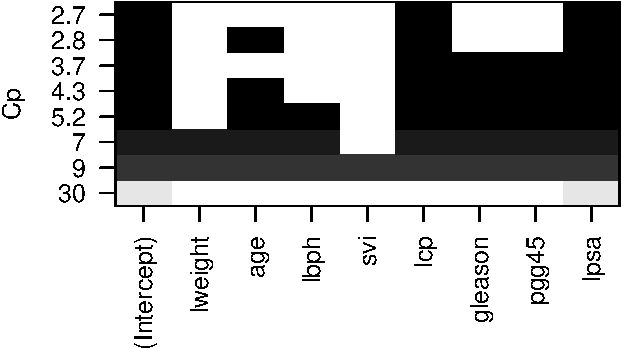
\includegraphics[width=0.5\linewidth]{Rcourse_files/figure-latex/all subset-1}

Things to note:

\begin{itemize}
\tightlist
\item
  The plot shows us which is the variable combination which is the best, i.e., has the smallest Cp.
\item
  Scanning over all variable subsets is impossible when the number of variables is large.
\end{itemize}

Instead of the Cp criterion, we now compute the train and test errors for all the possible predictor subsets\footnote{Example taken from \url{https://lagunita.stanford.edu/c4x/HumanitiesScience/StatLearning/asset/ch6.html}}.
In the resulting plot we can see overfitting in action.

\begin{Shaded}
\begin{Highlighting}[]
\NormalTok{model.n <-}\StringTok{ }\NormalTok{regfit.full }\OperatorTok\StringTok{ }\NormalTok{summary }\OperatorTok\StringTok{ }\NormalTok{length}
\NormalTok{X.train.named <-}\StringTok{ }\KeywordTok{model.matrix}\NormalTok{(lcavol }\OperatorTok{~}\StringTok{ }\NormalTok{., }\DataTypeTok{data =}\NormalTok{ prostate.train ) }
\NormalTok{X.test.named <-}\StringTok{ }\KeywordTok{model.matrix}\NormalTok{(lcavol }\OperatorTok{~}\StringTok{ }\NormalTok{., }\DataTypeTok{data =}\NormalTok{ prostate.test ) }

\NormalTok{val.errors <-}\StringTok{ }\KeywordTok{rep}\NormalTok{(}\OtherTok{NA}\NormalTok{, model.n)}
\NormalTok{train.errors <-}\StringTok{ }\KeywordTok{rep}\NormalTok{(}\OtherTok{NA}\NormalTok{, model.n)}
\ControlFlowTok{for}\NormalTok{ (i }\ControlFlowTok{in} \DecValTok{1}\OperatorTok{:}\NormalTok{model.n) \{}
\NormalTok{    coefi <-}\StringTok{ }\KeywordTok{coef}\NormalTok{(regfit.full, }\DataTypeTok{id =}\NormalTok{ i) }\CommentTok{# exctract coefficients of i'th model}
    
\NormalTok{    pred <-}\StringTok{  }\NormalTok{X.train.named[, }\KeywordTok{names}\NormalTok{(coefi)] }\OperatorTok\StringTok{ }\NormalTok{coefi }\CommentTok{# make in-sample predictions}
\NormalTok{    train.errors[i] <-}\StringTok{ }\KeywordTok{MSE}\NormalTok{(y.train }\OperatorTok{-}\StringTok{ }\NormalTok{pred) }\CommentTok{# train errors}

\NormalTok{    pred <-}\StringTok{  }\NormalTok{X.test.named[, }\KeywordTok{names}\NormalTok{(coefi)] }\OperatorTok\StringTok{ }\NormalTok{coefi }\CommentTok{# make out-of-sample predictions}
\NormalTok{    val.errors[i] <-}\StringTok{ }\KeywordTok{MSE}\NormalTok{(y.test }\OperatorTok{-}\StringTok{ }\NormalTok{pred) }\CommentTok{# test errors}
\NormalTok{\}}
\end{Highlighting}
\end{Shaded}

Plotting results.

\begin{Shaded}
\begin{Highlighting}[]
\KeywordTok{plot}\NormalTok{(train.errors, }\DataTypeTok{ylab =} \StringTok{"MSE"}\NormalTok{, }\DataTypeTok{pch =} \DecValTok{19}\NormalTok{, }\DataTypeTok{type =} \StringTok{"o"}\NormalTok{)}
\KeywordTok{points}\NormalTok{(val.errors, }\DataTypeTok{pch =} \DecValTok{19}\NormalTok{, }\DataTypeTok{type =} \StringTok{"b"}\NormalTok{, }\DataTypeTok{col=}\StringTok{"blue"}\NormalTok{)}
\KeywordTok{legend}\NormalTok{(}\StringTok{"topright"}\NormalTok{, }
       \DataTypeTok{legend =} \KeywordTok{c}\NormalTok{(}\StringTok{"Training"}\NormalTok{, }\StringTok{"Validation"}\NormalTok{), }
       \DataTypeTok{col =} \KeywordTok{c}\NormalTok{(}\StringTok{"black"}\NormalTok{, }\StringTok{"blue"}\NormalTok{), }
       \DataTypeTok{pch =} \DecValTok{19}\NormalTok{)}
\end{Highlighting}
\end{Shaded}

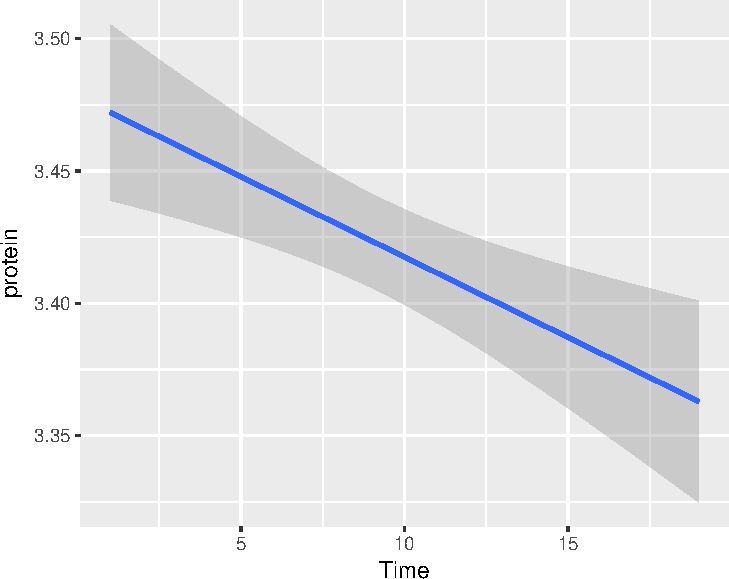
\includegraphics[width=0.5\linewidth]{Rcourse_files/figure-latex/unnamed-chunk-239-1}

Checking all possible models is computationally very hard.
\emph{Forward selection} is a greedy approach that adds one variable at a time.

\begin{Shaded}
\begin{Highlighting}[]
\NormalTok{ols}\FloatTok{.0}\NormalTok{ <-}\StringTok{ }\KeywordTok{lm}\NormalTok{(lcavol}\OperatorTok{~}\DecValTok{1}\NormalTok{ ,}\DataTypeTok{data =}\NormalTok{ prostate.train)}
\NormalTok{model.scope <-}\StringTok{ }\KeywordTok{list}\NormalTok{(}\DataTypeTok{upper=}\NormalTok{ols}\FloatTok{.1}\NormalTok{, }\DataTypeTok{lower=}\NormalTok{ols}\FloatTok{.0}\NormalTok{)}
\KeywordTok{step}\NormalTok{(ols}\FloatTok{.0}\NormalTok{, }\DataTypeTok{scope=}\NormalTok{model.scope, }\DataTypeTok{direction=}\StringTok{'forward'}\NormalTok{, }\DataTypeTok{trace =} \OtherTok{TRUE}\NormalTok{)}
\end{Highlighting}
\end{Shaded}

\begin{verbatim}
## Start:  AIC=30.1
## lcavol ~ 1
## 
##           Df Sum of Sq     RSS     AIC
## + lpsa     1    54.776  47.130 -19.570
## + lcp      1    48.805  53.101 -11.578
## + svi      1    35.829  66.077   3.071
## + pgg45    1    23.789  78.117  14.285
## + gleason  1    18.529  83.377  18.651
## + lweight  1     9.186  92.720  25.768
## + age      1     8.354  93.552  26.366
## <none>                 101.906  30.097
## + lbph     1     0.407 101.499  31.829
## 
## Step:  AIC=-19.57
## lcavol ~ lpsa
## 
##           Df Sum of Sq    RSS     AIC
## + lcp      1   14.8895 32.240 -43.009
## + svi      1    5.0373 42.093 -25.143
## + gleason  1    3.5500 43.580 -22.817
## + pgg45    1    3.0503 44.080 -22.053
## + lbph     1    1.8389 45.291 -20.236
## + age      1    1.5329 45.597 -19.785
## <none>                 47.130 -19.570
## + lweight  1    0.4106 46.719 -18.156
## 
## Step:  AIC=-43.01
## lcavol ~ lpsa + lcp
## 
##           Df Sum of Sq    RSS     AIC
## <none>                 32.240 -43.009
## + age      1   0.92315 31.317 -42.955
## + pgg45    1   0.29594 31.944 -41.627
## + gleason  1   0.21500 32.025 -41.457
## + lbph     1   0.13904 32.101 -41.298
## + lweight  1   0.05504 32.185 -41.123
## + svi      1   0.02069 32.220 -41.052
\end{verbatim}

\begin{verbatim}
## 
## Call:
## lm(formula = lcavol ~ lpsa + lcp, data = prostate.train)
## 
## Coefficients:
## (Intercept)         lpsa          lcp  
##     0.08798      0.53369      0.38879
\end{verbatim}

Things to note:

\begin{itemize}
\tightlist
\item
  By default \texttt{step} add variables according to the \href{https://en.wikipedia.org/wiki/Akaike_information_criterion}{AIC} criterion, which is a theory-driven unbiased risk estimator.
\item
  We need to tell \texttt{step} which is the smallest and largest models to consider using the \texttt{scope} argument.
\item
  \texttt{direction=\textquotesingle{}forward\textquotesingle{}} is used to ``grow'' from a small model. For ``shrinking'' a large model, use \texttt{direction=\textquotesingle{}backward\textquotesingle{}}, or the default \texttt{direction=\textquotesingle{}stepwise\textquotesingle{}}.
\end{itemize}

We now learn a linear predictor on the \texttt{spam} data using, a least squares loss, and train-test risk estimator.

\begin{Shaded}
\begin{Highlighting}[]
\CommentTok{# Train the predictor}
\NormalTok{ols}\FloatTok{.2}\NormalTok{ <-}\StringTok{ }\KeywordTok{lm}\NormalTok{(spam}\OperatorTok{~}\NormalTok{., }\DataTypeTok{data =}\NormalTok{ spam.train.dummy) }

\CommentTok{# make in-sample predictions}
\NormalTok{.predictions.train <-}\StringTok{ }\KeywordTok{predict}\NormalTok{(ols}\FloatTok{.2}\NormalTok{) }\OperatorTok{>}\StringTok{ }\FloatTok{0.5} 
\CommentTok{# inspect the confusion matrix}
\NormalTok{(confusion.train <-}\StringTok{ }\KeywordTok{table}\NormalTok{(}\DataTypeTok{prediction=}\NormalTok{.predictions.train, }\DataTypeTok{truth=}\NormalTok{spam.train.dummy}\OperatorTok{$}\NormalTok{spam)) }
\end{Highlighting}
\end{Shaded}

\begin{verbatim}
##           truth
## prediction    0    1
##      FALSE 1778  227
##      TRUE    66  980
\end{verbatim}

\begin{Shaded}
\begin{Highlighting}[]
\CommentTok{# compute the train (in sample) misclassification}
\KeywordTok{missclassification}\NormalTok{(confusion.train) }
\end{Highlighting}
\end{Shaded}

\begin{verbatim}
## [1] 0.09603409
\end{verbatim}

\begin{Shaded}
\begin{Highlighting}[]
\CommentTok{# make out-of-sample prediction}
\NormalTok{.predictions.test <-}\StringTok{ }\KeywordTok{predict}\NormalTok{(ols}\FloatTok{.2}\NormalTok{, }\DataTypeTok{newdata =}\NormalTok{ spam.test.dummy) }\OperatorTok{>}\StringTok{ }\FloatTok{0.5} 
\CommentTok{# inspect the confusion matrix}
\NormalTok{(confusion.test <-}\StringTok{ }\KeywordTok{table}\NormalTok{(}\DataTypeTok{prediction=}\NormalTok{.predictions.test, }\DataTypeTok{truth=}\NormalTok{spam.test.dummy}\OperatorTok{$}\NormalTok{spam))}
\end{Highlighting}
\end{Shaded}

\begin{verbatim}
##           truth
## prediction   0   1
##      FALSE 884 139
##      TRUE   60 467
\end{verbatim}

\begin{Shaded}
\begin{Highlighting}[]
\CommentTok{# compute the train (in sample) misclassification}
\KeywordTok{missclassification}\NormalTok{(confusion.test)}
\end{Highlighting}
\end{Shaded}

\begin{verbatim}
## [1] 0.1283871
\end{verbatim}

Things to note:

\begin{itemize}
\tightlist
\item
  I can use \texttt{lm} for categorical outcomes. \texttt{lm} will simply dummy-code the outcome.
\item
  A linear predictor trained on 0's and 1's will predict numbers. Think of these numbers as the probability of 1, and my prediction is the most probable class: \texttt{predicts()\textgreater{}0.5}.
\item
  The train error is smaller than the test error. This is overfitting in action.
\end{itemize}

The \texttt{glmnet} package is an excellent package that provides ridge, LASSO, and elastic net regularization, for all GLMs, so for linear models in particular.

\begin{Shaded}
\begin{Highlighting}[]
\KeywordTok{suppressMessages}\NormalTok{(}\KeywordTok{library}\NormalTok{(glmnet))}

\NormalTok{means <-}\StringTok{ }\KeywordTok{apply}\NormalTok{(X.train, }\DecValTok{2}\NormalTok{, mean)}
\NormalTok{sds <-}\StringTok{ }\KeywordTok{apply}\NormalTok{(X.train, }\DecValTok{2}\NormalTok{, sd)}
\NormalTok{X.train.scaled <-}\StringTok{ }\NormalTok{X.train }\OperatorTok\StringTok{ }\KeywordTok{sweep}\NormalTok{(}\DataTypeTok{MARGIN =} \DecValTok{2}\NormalTok{, }\DataTypeTok{STATS =}\NormalTok{ means, }\DataTypeTok{FUN =} \StringTok{`}\DataTypeTok{-}\StringTok{`}\NormalTok{) }\OperatorTok\StringTok{ }
\StringTok{  }\KeywordTok{sweep}\NormalTok{(}\DataTypeTok{MARGIN =} \DecValTok{2}\NormalTok{, }\DataTypeTok{STATS =}\NormalTok{ sds, }\DataTypeTok{FUN =} \StringTok{`}\DataTypeTok{/}\StringTok{`}\NormalTok{)}

\NormalTok{ridge}\FloatTok{.2}\NormalTok{ <-}\StringTok{ }\KeywordTok{glmnet}\NormalTok{(}\DataTypeTok{x=}\NormalTok{X.train.scaled, }\DataTypeTok{y=}\NormalTok{y.train, }\DataTypeTok{family =} \StringTok{'gaussian'}\NormalTok{, }\DataTypeTok{alpha =} \DecValTok{0}\NormalTok{)}

\CommentTok{# Train error:}
\KeywordTok{MSE}\NormalTok{( }\KeywordTok{predict}\NormalTok{(ridge}\FloatTok{.2}\NormalTok{, }\DataTypeTok{newx =}\NormalTok{X.train.scaled)}\OperatorTok{-}\StringTok{ }\NormalTok{y.train)}
\end{Highlighting}
\end{Shaded}

\begin{verbatim}
## [1] 1.006028
\end{verbatim}

\begin{Shaded}
\begin{Highlighting}[]
\CommentTok{# Test error:}
\NormalTok{X.test.scaled <-}\StringTok{ }\NormalTok{X.test }\OperatorTok\StringTok{ }\KeywordTok{sweep}\NormalTok{(}\DataTypeTok{MARGIN =} \DecValTok{2}\NormalTok{, }\DataTypeTok{STATS =}\NormalTok{ means, }\DataTypeTok{FUN =} \StringTok{`}\DataTypeTok{-}\StringTok{`}\NormalTok{) }\OperatorTok\StringTok{ }
\StringTok{  }\KeywordTok{sweep}\NormalTok{(}\DataTypeTok{MARGIN =} \DecValTok{2}\NormalTok{, }\DataTypeTok{STATS =}\NormalTok{ sds, }\DataTypeTok{FUN =} \StringTok{`}\DataTypeTok{/}\StringTok{`}\NormalTok{)}
\KeywordTok{MSE}\NormalTok{(}\KeywordTok{predict}\NormalTok{(ridge}\FloatTok{.2}\NormalTok{, }\DataTypeTok{newx =}\NormalTok{ X.test.scaled)}\OperatorTok{-}\StringTok{ }\NormalTok{y.test)}
\end{Highlighting}
\end{Shaded}

\begin{verbatim}
## [1] 0.7678264
\end{verbatim}

Things to note:

\begin{itemize}
\tightlist
\item
  The \texttt{alpha=0} parameters tells R to do ridge regression. Setting \(alpha=1\) will do LASSO, and any other value, with return an elastic net with appropriate weights.
\item
  The \texttt{family=\textquotesingle{}gaussian\textquotesingle{}} argument tells R to fit a linear model, with least squares loss.
\item
  Features for regularized predictors should be z-scored before learning.
\item
  We use the \texttt{sweep} function to z-score the predictors: we learn the z-scoring from the train set, and apply it to both the train and the test.
\item
  The test error is \textbf{smaller} than the train error. This may happen because risk estimators are random. Their variance may mask the overfitting.
\end{itemize}

We now use the LASSO penalty.

\begin{Shaded}
\begin{Highlighting}[]
\NormalTok{lasso}\FloatTok{.1}\NormalTok{ <-}\StringTok{ }\KeywordTok{glmnet}\NormalTok{(}\DataTypeTok{x=}\NormalTok{X.train.scaled, }\DataTypeTok{y=}\NormalTok{y.train, , }\DataTypeTok{family=}\StringTok{'gaussian'}\NormalTok{, }\DataTypeTok{alpha =} \DecValTok{1}\NormalTok{)}

\CommentTok{# Train error:}
\KeywordTok{MSE}\NormalTok{( }\KeywordTok{predict}\NormalTok{(lasso}\FloatTok{.1}\NormalTok{, }\DataTypeTok{newx =}\NormalTok{X.train.scaled)}\OperatorTok{-}\StringTok{ }\NormalTok{y.train)}
\end{Highlighting}
\end{Shaded}

\begin{verbatim}
## [1] 0.5525279
\end{verbatim}

\begin{Shaded}
\begin{Highlighting}[]
\CommentTok{# Test error:}
\KeywordTok{MSE}\NormalTok{( }\KeywordTok{predict}\NormalTok{(lasso}\FloatTok{.1}\NormalTok{, }\DataTypeTok{newx =}\NormalTok{ X.test.scaled)}\OperatorTok{-}\StringTok{ }\NormalTok{y.test)}
\end{Highlighting}
\end{Shaded}

\begin{verbatim}
## [1] 0.5211263
\end{verbatim}

We now use \texttt{glmnet} for classification.

\begin{Shaded}
\begin{Highlighting}[]
\NormalTok{means.spam <-}\StringTok{ }\KeywordTok{apply}\NormalTok{(X.train.spam, }\DecValTok{2}\NormalTok{, mean)}
\NormalTok{sds.spam <-}\StringTok{ }\KeywordTok{apply}\NormalTok{(X.train.spam, }\DecValTok{2}\NormalTok{, sd)}
\NormalTok{X.train.spam.scaled <-}\StringTok{ }\NormalTok{X.train.spam }\OperatorTok\StringTok{ }\KeywordTok{sweep}\NormalTok{(}\DataTypeTok{MARGIN =} \DecValTok{2}\NormalTok{, }\DataTypeTok{STATS =}\NormalTok{ means.spam, }\DataTypeTok{FUN =} \StringTok{`}\DataTypeTok{-}\StringTok{`}\NormalTok{) }\OperatorTok\StringTok{ }
\StringTok{  }\KeywordTok{sweep}\NormalTok{(}\DataTypeTok{MARGIN =} \DecValTok{2}\NormalTok{, }\DataTypeTok{STATS =}\NormalTok{ sds.spam, }\DataTypeTok{FUN =} \StringTok{`}\DataTypeTok{/}\StringTok{`}\NormalTok{) }\OperatorTok\StringTok{ }\NormalTok{as.matrix}

\NormalTok{logistic}\FloatTok{.2}\NormalTok{ <-}\StringTok{ }\KeywordTok{cv.glmnet}\NormalTok{(}\DataTypeTok{x=}\NormalTok{X.train.spam.scaled, }\DataTypeTok{y=}\NormalTok{y.train.spam, }\DataTypeTok{family =} \StringTok{"binomial"}\NormalTok{, }\DataTypeTok{alpha =} \DecValTok{0}\NormalTok{)}
\end{Highlighting}
\end{Shaded}

Things to note:

\begin{itemize}
\tightlist
\item
  We used \texttt{cv.glmnet} to do an automatic search for the optimal level of regularization (the \texttt{lambda} argument in \texttt{glmnet}) using V-fold CV.
\item
  Just like the \texttt{glm} function, \texttt{\textquotesingle{}family=\textquotesingle{}binomial\textquotesingle{}} is used for logistic regression.
\item
  We z-scored features so that they all have the same scale.
\item
  We set \texttt{alpha=0} for an \(l_2\) penalization of the coefficients of the logistic regression.
\end{itemize}

\begin{Shaded}
\begin{Highlighting}[]
\CommentTok{# Train confusion matrix:}
\NormalTok{.predictions.train <-}\StringTok{ }\KeywordTok{predict}\NormalTok{(logistic}\FloatTok{.2}\NormalTok{, }\DataTypeTok{newx =}\NormalTok{ X.train.spam.scaled, }\DataTypeTok{type =} \StringTok{'class'}\NormalTok{) }
\NormalTok{(confusion.train <-}\StringTok{ }\KeywordTok{table}\NormalTok{(}\DataTypeTok{prediction=}\NormalTok{.predictions.train, }\DataTypeTok{truth=}\NormalTok{spam.train}\OperatorTok{$}\NormalTok{spam))}
\end{Highlighting}
\end{Shaded}

\begin{verbatim}
##           truth
## prediction email spam
##      email  1778  167
##      spam     66 1040
\end{verbatim}

\begin{Shaded}
\begin{Highlighting}[]
\CommentTok{# Train misclassification error}
\KeywordTok{missclassification}\NormalTok{(confusion.train)}
\end{Highlighting}
\end{Shaded}

\begin{verbatim}
## [1] 0.0763684
\end{verbatim}

\begin{Shaded}
\begin{Highlighting}[]
\CommentTok{# Test confusion matrix:}
\NormalTok{X.test.spam.scaled <-}\StringTok{ }\NormalTok{X.test.spam }\OperatorTok\StringTok{ }\KeywordTok{sweep}\NormalTok{(}\DataTypeTok{MARGIN =} \DecValTok{2}\NormalTok{, }\DataTypeTok{STATS =}\NormalTok{ means.spam, }\DataTypeTok{FUN =} \StringTok{`}\DataTypeTok{-}\StringTok{`}\NormalTok{) }\OperatorTok\StringTok{ }
\StringTok{  }\KeywordTok{sweep}\NormalTok{(}\DataTypeTok{MARGIN =} \DecValTok{2}\NormalTok{, }\DataTypeTok{STATS =}\NormalTok{ sds.spam, }\DataTypeTok{FUN =} \StringTok{`}\DataTypeTok{/}\StringTok{`}\NormalTok{) }\OperatorTok\StringTok{ }\NormalTok{as.matrix}

\NormalTok{.predictions.test <-}\StringTok{ }\KeywordTok{predict}\NormalTok{(logistic}\FloatTok{.2}\NormalTok{, }\DataTypeTok{newx =}\NormalTok{ X.test.spam.scaled, }\DataTypeTok{type=}\StringTok{'class'}\NormalTok{) }
\NormalTok{(confusion.test <-}\StringTok{ }\KeywordTok{table}\NormalTok{(}\DataTypeTok{prediction=}\NormalTok{.predictions.test, }\DataTypeTok{truth=}\NormalTok{y.test.spam))}
\end{Highlighting}
\end{Shaded}

\begin{verbatim}
##           truth
## prediction email spam
##      email   885  110
##      spam     59  496
\end{verbatim}

\begin{Shaded}
\begin{Highlighting}[]
\CommentTok{# Test misclassification error:}
\KeywordTok{missclassification}\NormalTok{(confusion.test)}
\end{Highlighting}
\end{Shaded}

\begin{verbatim}
## [1] 0.1090323
\end{verbatim}

\hypertarget{svm}{%
\subsection{SVM}\label{svm}}

A support vector machine (SVM) is a linear hypothesis class with a particular loss function known as a \href{https://en.wikipedia.org/wiki/Hinge_loss}{hinge loss}.
We learn an SVM with the \texttt{svm} function from the \textbf{e1071} package, which is merely a wrapper for the \href{https://www.csie.ntu.edu.tw/~cjlin/libsvm/}{libsvm} C library; the most popular implementation of SVM today.

\begin{Shaded}
\begin{Highlighting}[]
\KeywordTok{library}\NormalTok{(e1071)}
\NormalTok{svm}\FloatTok{.1}\NormalTok{ <-}\StringTok{ }\KeywordTok{svm}\NormalTok{(spam}\OperatorTok{~}\NormalTok{., }\DataTypeTok{data =}\NormalTok{ spam.train, }\DataTypeTok{kernel=}\StringTok{'linear'}\NormalTok{)}

\CommentTok{# Train confusion matrix:}
\NormalTok{.predictions.train <-}\StringTok{ }\KeywordTok{predict}\NormalTok{(svm}\FloatTok{.1}\NormalTok{) }
\NormalTok{(confusion.train <-}\StringTok{ }\KeywordTok{table}\NormalTok{(}\DataTypeTok{prediction=}\NormalTok{.predictions.train, }\DataTypeTok{truth=}\NormalTok{spam.train}\OperatorTok{$}\NormalTok{spam))}
\end{Highlighting}
\end{Shaded}

\begin{verbatim}
##           truth
## prediction email spam
##      email  1774  106
##      spam     70 1101
\end{verbatim}

\begin{Shaded}
\begin{Highlighting}[]
\KeywordTok{missclassification}\NormalTok{(confusion.train)}
\end{Highlighting}
\end{Shaded}

\begin{verbatim}
## [1] 0.057686
\end{verbatim}

\begin{Shaded}
\begin{Highlighting}[]
\CommentTok{# Test confusion matrix:}
\NormalTok{.predictions.test <-}\StringTok{ }\KeywordTok{predict}\NormalTok{(svm}\FloatTok{.1}\NormalTok{, }\DataTypeTok{newdata =}\NormalTok{ spam.test) }
\NormalTok{(confusion.test <-}\StringTok{ }\KeywordTok{table}\NormalTok{(}\DataTypeTok{prediction=}\NormalTok{.predictions.test, }\DataTypeTok{truth=}\NormalTok{spam.test}\OperatorTok{$}\NormalTok{spam))}
\end{Highlighting}
\end{Shaded}

\begin{verbatim}
##           truth
## prediction email spam
##      email   876   75
##      spam     68  531
\end{verbatim}

\begin{Shaded}
\begin{Highlighting}[]
\KeywordTok{missclassification}\NormalTok{(confusion.test)}
\end{Highlighting}
\end{Shaded}

\begin{verbatim}
## [1] 0.09225806
\end{verbatim}

We can also use SVM for regression.

\begin{Shaded}
\begin{Highlighting}[]
\NormalTok{svm}\FloatTok{.2}\NormalTok{ <-}\StringTok{ }\KeywordTok{svm}\NormalTok{(lcavol}\OperatorTok{~}\NormalTok{., }\DataTypeTok{data =}\NormalTok{ prostate.train, }\DataTypeTok{kernel=}\StringTok{'linear'}\NormalTok{)}

\CommentTok{# Train error:}
\KeywordTok{MSE}\NormalTok{( }\KeywordTok{predict}\NormalTok{(svm}\FloatTok{.2}\NormalTok{)}\OperatorTok{-}\StringTok{ }\NormalTok{prostate.train}\OperatorTok{$}\NormalTok{lcavol)}
\end{Highlighting}
\end{Shaded}

\begin{verbatim}
## [1] 0.4488577
\end{verbatim}

\begin{Shaded}
\begin{Highlighting}[]
\CommentTok{# Test error:}
\KeywordTok{MSE}\NormalTok{( }\KeywordTok{predict}\NormalTok{(svm}\FloatTok{.2}\NormalTok{, }\DataTypeTok{newdata =}\NormalTok{ prostate.test)}\OperatorTok{-}\StringTok{ }\NormalTok{prostate.test}\OperatorTok{$}\NormalTok{lcavol)}
\end{Highlighting}
\end{Shaded}

\begin{verbatim}
## [1] 0.5547759
\end{verbatim}

Things to note:

\begin{itemize}
\tightlist
\item
  The use of \texttt{kernel=\textquotesingle{}linear\textquotesingle{}} forces the predictor to be linear. Various hypothesis classes may be used by changing the \texttt{kernel} argument.
\end{itemize}

\hypertarget{neural-nets}{%
\subsection{Neural Nets}\label{neural-nets}}

Neural nets (non deep) can be fitted, for example, with the \texttt{nnet} function in the \textbf{nnet} package.
We start with a nnet regression.

\begin{Shaded}
\begin{Highlighting}[]
\KeywordTok{library}\NormalTok{(nnet)}
\NormalTok{nnet}\FloatTok{.1}\NormalTok{ <-}\StringTok{ }\KeywordTok{nnet}\NormalTok{(lcavol}\OperatorTok{~}\NormalTok{., }\DataTypeTok{size=}\DecValTok{20}\NormalTok{, }\DataTypeTok{data=}\NormalTok{prostate.train, }\DataTypeTok{rang =} \FloatTok{0.1}\NormalTok{, }\DataTypeTok{decay =} \FloatTok{5e-4}\NormalTok{, }\DataTypeTok{maxit =} \DecValTok{1000}\NormalTok{, }\DataTypeTok{trace=}\OtherTok{FALSE}\NormalTok{)}

\CommentTok{# Train error:}
\KeywordTok{MSE}\NormalTok{( }\KeywordTok{predict}\NormalTok{(nnet}\FloatTok{.1}\NormalTok{)}\OperatorTok{-}\StringTok{ }\NormalTok{prostate.train}\OperatorTok{$}\NormalTok{lcavol)}
\end{Highlighting}
\end{Shaded}

\begin{verbatim}
## [1] 1.177099
\end{verbatim}

\begin{Shaded}
\begin{Highlighting}[]
\CommentTok{# Test error:}
\KeywordTok{MSE}\NormalTok{( }\KeywordTok{predict}\NormalTok{(nnet}\FloatTok{.1}\NormalTok{, }\DataTypeTok{newdata =}\NormalTok{ prostate.test)}\OperatorTok{-}\StringTok{ }\NormalTok{prostate.test}\OperatorTok{$}\NormalTok{lcavol)}
\end{Highlighting}
\end{Shaded}

\begin{verbatim}
## [1] 1.21175
\end{verbatim}

And nnet classification.

\begin{Shaded}
\begin{Highlighting}[]
\NormalTok{nnet}\FloatTok{.2}\NormalTok{ <-}\StringTok{ }\KeywordTok{nnet}\NormalTok{(spam}\OperatorTok{~}\NormalTok{., }\DataTypeTok{size=}\DecValTok{5}\NormalTok{, }\DataTypeTok{data=}\NormalTok{spam.train, }\DataTypeTok{rang =} \FloatTok{0.1}\NormalTok{, }\DataTypeTok{decay =} \FloatTok{5e-4}\NormalTok{, }\DataTypeTok{maxit =} \DecValTok{1000}\NormalTok{, }\DataTypeTok{trace=}\OtherTok{FALSE}\NormalTok{)}

\CommentTok{# Train confusion matrix:}
\NormalTok{.predictions.train <-}\StringTok{ }\KeywordTok{predict}\NormalTok{(nnet}\FloatTok{.2}\NormalTok{, }\DataTypeTok{type=}\StringTok{'class'}\NormalTok{) }
\NormalTok{(confusion.train <-}\StringTok{ }\KeywordTok{table}\NormalTok{(}\DataTypeTok{prediction=}\NormalTok{.predictions.train, }\DataTypeTok{truth=}\NormalTok{spam.train}\OperatorTok{$}\NormalTok{spam))}
\end{Highlighting}
\end{Shaded}

\begin{verbatim}
##           truth
## prediction email spam
##      email  1806   59
##      spam     38 1148
\end{verbatim}

\begin{Shaded}
\begin{Highlighting}[]
\KeywordTok{missclassification}\NormalTok{(confusion.train)}
\end{Highlighting}
\end{Shaded}

\begin{verbatim}
## [1] 0.03179285
\end{verbatim}

\begin{Shaded}
\begin{Highlighting}[]
\CommentTok{# Test confusion matrix:}
\NormalTok{.predictions.test <-}\StringTok{ }\KeywordTok{predict}\NormalTok{(nnet}\FloatTok{.2}\NormalTok{, }\DataTypeTok{newdata =}\NormalTok{ spam.test, }\DataTypeTok{type=}\StringTok{'class'}\NormalTok{) }
\NormalTok{(confusion.test <-}\StringTok{ }\KeywordTok{table}\NormalTok{(}\DataTypeTok{prediction=}\NormalTok{.predictions.test, }\DataTypeTok{truth=}\NormalTok{spam.test}\OperatorTok{$}\NormalTok{spam))}
\end{Highlighting}
\end{Shaded}

\begin{verbatim}
##           truth
## prediction email spam
##      email   897   64
##      spam     47  542
\end{verbatim}

\begin{Shaded}
\begin{Highlighting}[]
\KeywordTok{missclassification}\NormalTok{(confusion.test)}
\end{Highlighting}
\end{Shaded}

\begin{verbatim}
## [1] 0.0716129
\end{verbatim}

\hypertarget{deep-neural-nets}{%
\subsubsection{Deep Neural Nets}\label{deep-neural-nets}}

Deep-Neural-Networks are undoubtedly the ``hottest'' topic in machine-learning and artificial intelligence.
This real is too vast to be covered in this text.
We merely refer the reader to the \href{https://cran.r-project.org/package=tensorflow}{tensorflow} package documentation as a starting point.

\hypertarget{trees}{%
\subsection{Classification and Regression Trees (CART)}\label{trees}}

A CART, is not a linear hypothesis class.
It partitions the feature space \(\mathcal{X}\), thus creating a set of if-then rules for prediction or classification.
It is thus particularly useful when you believe that the predicted classes may change abruptly with small changes in \(x\).

\hypertarget{rpart}{%
\subsubsection{The rpart Package}\label{rpart}}

This view clarifies the name of the function \texttt{rpart}, which \emph{recursively partitions} the feature space.

We start with a regression tree.

\begin{Shaded}
\begin{Highlighting}[]
\KeywordTok{library}\NormalTok{(rpart)}
\NormalTok{tree}\FloatTok{.1}\NormalTok{ <-}\StringTok{ }\KeywordTok{rpart}\NormalTok{(lcavol}\OperatorTok{~}\NormalTok{., }\DataTypeTok{data=}\NormalTok{prostate.train)}

\CommentTok{# Train error:}
\KeywordTok{MSE}\NormalTok{( }\KeywordTok{predict}\NormalTok{(tree}\FloatTok{.1}\NormalTok{)}\OperatorTok{-}\StringTok{ }\NormalTok{prostate.train}\OperatorTok{$}\NormalTok{lcavol)}
\end{Highlighting}
\end{Shaded}

\begin{verbatim}
## [1] 0.4909568
\end{verbatim}

\begin{Shaded}
\begin{Highlighting}[]
\CommentTok{# Test error:}
\KeywordTok{MSE}\NormalTok{( }\KeywordTok{predict}\NormalTok{(tree}\FloatTok{.1}\NormalTok{, }\DataTypeTok{newdata =}\NormalTok{ prostate.test)}\OperatorTok{-}\StringTok{ }\NormalTok{prostate.test}\OperatorTok{$}\NormalTok{lcavol)}
\end{Highlighting}
\end{Shaded}

\begin{verbatim}
## [1] 0.5623316
\end{verbatim}

We can use the \textbf{rpart.plot} package to visualize and interpret the predictor.

\begin{Shaded}
\begin{Highlighting}[]
\NormalTok{rpart.plot}\OperatorTok{::}\KeywordTok{rpart.plot}\NormalTok{(tree}\FloatTok{.1}\NormalTok{)}
\end{Highlighting}
\end{Shaded}

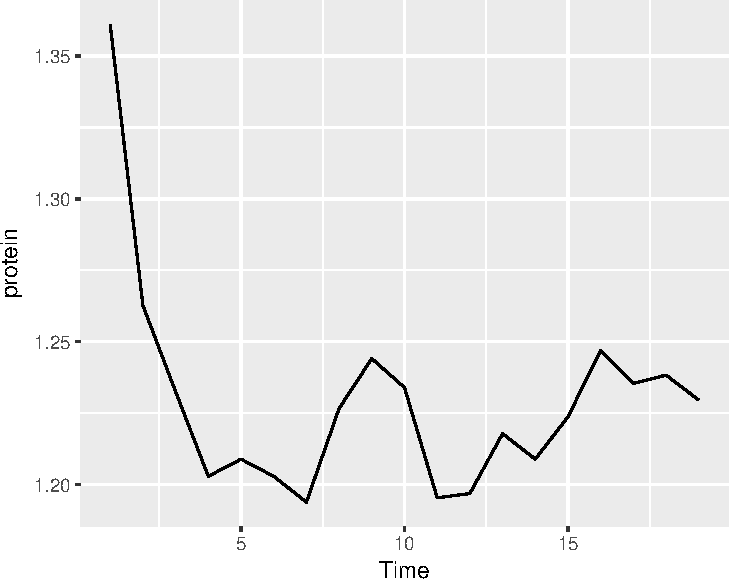
\includegraphics[width=0.5\linewidth]{Rcourse_files/figure-latex/unnamed-chunk-244-1}

Or the newer \href{https://cran.r-project.org/web/packages/ggparty/vignettes/ggparty-graphic-partying.html}{ggparty} package, for trees fitted with the \href{https://cran.r-project.org/package=party}{party} package.

Trees are very prone to overfitting.
To avoid this, we reduce a tree's complexity by \emph{pruning} it.
This is done with the \texttt{rpart::prune} function (not demonstrated herein).

We now fit a classification tree.

\begin{Shaded}
\begin{Highlighting}[]
\NormalTok{tree}\FloatTok{.2}\NormalTok{ <-}\StringTok{ }\KeywordTok{rpart}\NormalTok{(spam}\OperatorTok{~}\NormalTok{., }\DataTypeTok{data=}\NormalTok{spam.train)}

\CommentTok{# Train confusion matrix:}
\NormalTok{.predictions.train <-}\StringTok{ }\KeywordTok{predict}\NormalTok{(tree}\FloatTok{.2}\NormalTok{, }\DataTypeTok{type=}\StringTok{'class'}\NormalTok{) }
\NormalTok{(confusion.train <-}\StringTok{ }\KeywordTok{table}\NormalTok{(}\DataTypeTok{prediction=}\NormalTok{.predictions.train, }\DataTypeTok{truth=}\NormalTok{spam.train}\OperatorTok{$}\NormalTok{spam))}
\end{Highlighting}
\end{Shaded}

\begin{verbatim}
##           truth
## prediction email spam
##      email  1785  217
##      spam     59  990
\end{verbatim}

\begin{Shaded}
\begin{Highlighting}[]
\KeywordTok{missclassification}\NormalTok{(confusion.train)}
\end{Highlighting}
\end{Shaded}

\begin{verbatim}
## [1] 0.09046214
\end{verbatim}

\begin{Shaded}
\begin{Highlighting}[]
\CommentTok{# Test confusion matrix:}
\NormalTok{.predictions.test <-}\StringTok{ }\KeywordTok{predict}\NormalTok{(tree}\FloatTok{.2}\NormalTok{, }\DataTypeTok{newdata =}\NormalTok{ spam.test, }\DataTypeTok{type=}\StringTok{'class'}\NormalTok{) }
\NormalTok{(confusion.test <-}\StringTok{ }\KeywordTok{table}\NormalTok{(}\DataTypeTok{prediction=}\NormalTok{.predictions.test, }\DataTypeTok{truth=}\NormalTok{spam.test}\OperatorTok{$}\NormalTok{spam))}
\end{Highlighting}
\end{Shaded}

\begin{verbatim}
##           truth
## prediction email spam
##      email   906  125
##      spam     38  481
\end{verbatim}

\begin{Shaded}
\begin{Highlighting}[]
\KeywordTok{missclassification}\NormalTok{(confusion.test)}
\end{Highlighting}
\end{Shaded}

\begin{verbatim}
## [1] 0.1051613
\end{verbatim}

\hypertarget{caret}{%
\subsubsection{The caret Package}\label{caret}}

In the \textbf{rpart} package {[}\ref{rpart}{]} we grow a tree with one function, and then prune it with another.\\
The \textbf{caret} implementation of trees does both with a single function.
We demonstrate the package in the context of trees, but it is actually a very convenient wrapper for many learning algorithms; \href{http://topepo.github.io/caret/available-models.html\#}{237(!)}
learning algorithms to be precise.

\begin{Shaded}
\begin{Highlighting}[]
\KeywordTok{library}\NormalTok{(caret)}
\CommentTok{# Control some training parameters}
\NormalTok{train.control <-}\StringTok{ }\KeywordTok{trainControl}\NormalTok{(}\DataTypeTok{method =} \StringTok{"cv"}\NormalTok{,}
                           \DataTypeTok{number =} \DecValTok{10}\NormalTok{)}

\NormalTok{tree}\FloatTok{.3}\NormalTok{ <-}\StringTok{ }\KeywordTok{train}\NormalTok{(lcavol}\OperatorTok{~}\NormalTok{., }\DataTypeTok{data=}\NormalTok{prostate.train, }
                \DataTypeTok{method=}\StringTok{'rpart'}\NormalTok{, }
                \DataTypeTok{trControl=}\NormalTok{train.control)}
\NormalTok{tree}\FloatTok{.3}
\end{Highlighting}
\end{Shaded}

\begin{verbatim}
## CART 
## 
## 67 samples
##  8 predictor
## 
## No pre-processing
## Resampling: Cross-Validated (10 fold) 
## Summary of sample sizes: 61, 60, 59, 60, 60, 61, ... 
## Resampling results across tuning parameters:
## 
##   cp          RMSE       Rsquared   MAE      
##   0.04682924  0.9118374  0.5026786  0.7570798
##   0.14815712  0.9899308  0.4690557  0.7972803
##   0.44497285  1.1912870  0.3264172  1.0008574
## 
## RMSE was used to select the optimal model using the smallest value.
## The final value used for the model was cp = 0.04682924.
\end{verbatim}

\begin{Shaded}
\begin{Highlighting}[]
\CommentTok{# Train error:}
\KeywordTok{MSE}\NormalTok{( }\KeywordTok{predict}\NormalTok{(tree}\FloatTok{.3}\NormalTok{)}\OperatorTok{-}\StringTok{ }\NormalTok{prostate.train}\OperatorTok{$}\NormalTok{lcavol)}
\end{Highlighting}
\end{Shaded}

\begin{verbatim}
## [1] 0.6188435
\end{verbatim}

\begin{Shaded}
\begin{Highlighting}[]
\CommentTok{# Test error:}
\KeywordTok{MSE}\NormalTok{( }\KeywordTok{predict}\NormalTok{(tree}\FloatTok{.3}\NormalTok{, }\DataTypeTok{newdata =}\NormalTok{ prostate.test)}\OperatorTok{-}\StringTok{ }\NormalTok{prostate.test}\OperatorTok{$}\NormalTok{lcavol)}
\end{Highlighting}
\end{Shaded}

\begin{verbatim}
## [1] 0.545632
\end{verbatim}

Things to note:

\begin{itemize}
\tightlist
\item
  A tree was trained because of the \texttt{method=\textquotesingle{}rpart\textquotesingle{}} argument. Many other predictive models are available. See \href{http://topepo.github.io/caret/available-models.html}{here}.
\item
  The pruning of the tree was done automatically by the \texttt{caret::train()} function.
\item
  The method of pruning is controlled by a control object, generated with the \texttt{caret::trainControl()} function. In our case, \texttt{method\ =\ "cv"} for cross-validation, and \texttt{number\ =\ 10} for 10-folds.
\item
  The train error is larger than the test error. This is possible because the tree is not an ERM on the train data. Rather, it is an ERM on the variations of the data generated by the cross-validation process.
\end{itemize}

\hypertarget{parsnip}{%
\subsubsection{The parsnip package}\label{parsnip}}

At this point you may have noted that different R packages have differet interfaces to specify and fit models.
Wouldn't it be nice to have a unified language that allows to specify a model, indpendently of the undelying fitting libraries?
This is percisely the purpose of \href{https://github.com/tidymodels/parsnip}{parsnip}, created by \href{https://twitter.com/topepos}{Max Kuhn}, the author of \textbf{caret}.
With parsnip, you specify a model, save it, and can later dispatch it to fitting with \textbf{lm}, \textbf{glmnet}, \textbf{Spark}, or other fitting libraries.
This is much like \textbf{ggplot2}, where you specify a plot, save it, and dispatch it for printing using \emph{print()}.

TODO: add code examples.

\hypertarget{k-nearest-neighbour-knn}{%
\subsection{K-nearest neighbour (KNN)}\label{k-nearest-neighbour-knn}}

KNN is not an ERM problem.
In the KNN algorithm, a prediction at some \(x\) is made based on the \(y\) is it neighbors.
This means that:

\begin{itemize}
\tightlist
\item
  KNN is an \href{https://en.wikipedia.org/wiki/Instance-based_learning}{Instance Based} learning algorithm where we do not learn the values of some parametric function, but rather, need the original sample to make predictions. This has many implications when dealing with ``BigData''.
\item
  It may only be applied in spaces with known/defined metric. It is thus harder to apply in the presence of missing values, or in ``string-spaces'', ``genome-spaces'', etc. where no canonical metric exists.
\end{itemize}

KNN is so fundamental that we show how to fit such a hypothesis class, even if it not an ERM algorithm.
Is KNN any good?
I have never seen a learning problem where KNN beats other methods. Others claim differently.

\begin{Shaded}
\begin{Highlighting}[]
\KeywordTok{library}\NormalTok{(class)}
\NormalTok{knn}\FloatTok{.1}\NormalTok{ <-}\StringTok{ }\KeywordTok{knn}\NormalTok{(}\DataTypeTok{train =}\NormalTok{ X.train.spam.scaled, }\DataTypeTok{test =}\NormalTok{ X.test.spam.scaled, }\DataTypeTok{cl =}\NormalTok{y.train.spam, }\DataTypeTok{k =} \DecValTok{1}\NormalTok{)}

\CommentTok{# Test confusion matrix:}
\NormalTok{.predictions.test <-}\StringTok{ }\NormalTok{knn}\FloatTok{.1} 
\NormalTok{(confusion.test <-}\StringTok{ }\KeywordTok{table}\NormalTok{(}\DataTypeTok{prediction=}\NormalTok{.predictions.test, }\DataTypeTok{truth=}\NormalTok{spam.test}\OperatorTok{$}\NormalTok{spam))}
\end{Highlighting}
\end{Shaded}

\begin{verbatim}
##           truth
## prediction email spam
##      email   856   86
##      spam     88  520
\end{verbatim}

\begin{Shaded}
\begin{Highlighting}[]
\KeywordTok{missclassification}\NormalTok{(confusion.test)}
\end{Highlighting}
\end{Shaded}

\begin{verbatim}
## [1] 0.1122581
\end{verbatim}

\hypertarget{linear-discriminant-analysis-lda}{%
\subsection{Linear Discriminant Analysis (LDA)}\label{linear-discriminant-analysis-lda}}

LDA is equivalent to least squares classification \ref{least-squares}.
This means that we actually did LDA when we used \texttt{lm} for binary classification (feel free to compare the confusion matrices).
There are, however, some dedicated functions to fit it which we now introduce.

\begin{Shaded}
\begin{Highlighting}[]
\KeywordTok{library}\NormalTok{(MASS)}
\NormalTok{lda}\FloatTok{.1}\NormalTok{ <-}\StringTok{ }\KeywordTok{lda}\NormalTok{(spam}\OperatorTok{~}\NormalTok{., spam.train)}

\CommentTok{# Train confusion matrix:}
\NormalTok{.predictions.train <-}\StringTok{ }\KeywordTok{predict}\NormalTok{(lda}\FloatTok{.1}\NormalTok{)}\OperatorTok{$}\NormalTok{class}
\NormalTok{(confusion.train <-}\StringTok{ }\KeywordTok{table}\NormalTok{(}\DataTypeTok{prediction=}\NormalTok{.predictions.train, }\DataTypeTok{truth=}\NormalTok{spam.train}\OperatorTok{$}\NormalTok{spam))}
\end{Highlighting}
\end{Shaded}

\begin{verbatim}
##           truth
## prediction email spam
##      email  1776  227
##      spam     68  980
\end{verbatim}

\begin{Shaded}
\begin{Highlighting}[]
\KeywordTok{missclassification}\NormalTok{(confusion.train)}
\end{Highlighting}
\end{Shaded}

\begin{verbatim}
## [1] 0.09668961
\end{verbatim}

\begin{Shaded}
\begin{Highlighting}[]
\CommentTok{# Test confusion matrix:}
\NormalTok{.predictions.test <-}\StringTok{ }\KeywordTok{predict}\NormalTok{(lda}\FloatTok{.1}\NormalTok{, }\DataTypeTok{newdata =}\NormalTok{ spam.test)}\OperatorTok{$}\NormalTok{class}
\NormalTok{(confusion.test <-}\StringTok{ }\KeywordTok{table}\NormalTok{(}\DataTypeTok{prediction=}\NormalTok{.predictions.test, }\DataTypeTok{truth=}\NormalTok{spam.test}\OperatorTok{$}\NormalTok{spam))}
\end{Highlighting}
\end{Shaded}

\begin{verbatim}
##           truth
## prediction email spam
##      email   884  138
##      spam     60  468
\end{verbatim}

\begin{Shaded}
\begin{Highlighting}[]
\KeywordTok{missclassification}\NormalTok{(confusion.test)}
\end{Highlighting}
\end{Shaded}

\begin{verbatim}
## [1] 0.1277419
\end{verbatim}

\hypertarget{naive-bayes}{%
\subsection{Naive Bayes}\label{naive-bayes}}

Naive-Bayes can be thought of LDA, i.e.~linear regression, where predictors are assume to be uncorrelated.
Predictions may be very good and certainly very fast, even if this assumption is not true.

\begin{Shaded}
\begin{Highlighting}[]
\KeywordTok{library}\NormalTok{(e1071)}
\NormalTok{nb}\FloatTok{.1}\NormalTok{ <-}\StringTok{ }\KeywordTok{naiveBayes}\NormalTok{(spam}\OperatorTok{~}\NormalTok{., }\DataTypeTok{data =}\NormalTok{ spam.train)}

\CommentTok{# Train confusion matrix:}
\NormalTok{.predictions.train <-}\StringTok{ }\KeywordTok{predict}\NormalTok{(nb}\FloatTok{.1}\NormalTok{, }\DataTypeTok{newdata =}\NormalTok{ spam.train)}
\NormalTok{(confusion.train <-}\StringTok{ }\KeywordTok{table}\NormalTok{(}\DataTypeTok{prediction=}\NormalTok{.predictions.train, }\DataTypeTok{truth=}\NormalTok{spam.train}\OperatorTok{$}\NormalTok{spam))}
\end{Highlighting}
\end{Shaded}

\begin{verbatim}
##           truth
## prediction email spam
##      email  1025   55
##      spam    819 1152
\end{verbatim}

\begin{Shaded}
\begin{Highlighting}[]
\KeywordTok{missclassification}\NormalTok{(confusion.train)}
\end{Highlighting}
\end{Shaded}

\begin{verbatim}
## [1] 0.2864635
\end{verbatim}

\begin{Shaded}
\begin{Highlighting}[]
\CommentTok{# Test confusion matrix:}
\NormalTok{.predictions.test <-}\StringTok{ }\KeywordTok{predict}\NormalTok{(nb}\FloatTok{.1}\NormalTok{, }\DataTypeTok{newdata =}\NormalTok{ spam.test)}
\NormalTok{(confusion.test <-}\StringTok{ }\KeywordTok{table}\NormalTok{(}\DataTypeTok{prediction=}\NormalTok{.predictions.test, }\DataTypeTok{truth=}\NormalTok{spam.test}\OperatorTok{$}\NormalTok{spam))}
\end{Highlighting}
\end{Shaded}

\begin{verbatim}
##           truth
## prediction email spam
##      email   484   42
##      spam    460  564
\end{verbatim}

\begin{Shaded}
\begin{Highlighting}[]
\KeywordTok{missclassification}\NormalTok{(confusion.test)}
\end{Highlighting}
\end{Shaded}

\begin{verbatim}
## [1] 0.323871
\end{verbatim}

\hypertarget{random-forrest}{%
\subsection{Random Forrest}\label{random-forrest}}

A Random Forrest is one of the most popular supervised learning algorithms.
It it an extremely successful algorithm, with very few tuning parameters, and easily parallelizable (thus salable to massive datasets).

\begin{Shaded}
\begin{Highlighting}[]
\CommentTok{# Control some training parameters}
\NormalTok{train.control <-}\StringTok{ }\KeywordTok{trainControl}\NormalTok{(}\DataTypeTok{method =} \StringTok{"cv"}\NormalTok{, }\DataTypeTok{number =} \DecValTok{10}\NormalTok{)}
\NormalTok{rf}\FloatTok{.1}\NormalTok{ <-}\StringTok{ }\NormalTok{caret}\OperatorTok{::}\KeywordTok{train}\NormalTok{(lcavol}\OperatorTok{~}\NormalTok{., }\DataTypeTok{data=}\NormalTok{prostate.train, }
                \DataTypeTok{method=}\StringTok{'rf'}\NormalTok{, }
                \DataTypeTok{trControl=}\NormalTok{train.control)}
\NormalTok{rf}\FloatTok{.1}
\end{Highlighting}
\end{Shaded}

\begin{verbatim}
## Random Forest 
## 
## 67 samples
##  8 predictor
## 
## No pre-processing
## Resampling: Cross-Validated (10 fold) 
## Summary of sample sizes: 62, 59, 60, 60, 59, 61, ... 
## Resampling results across tuning parameters:
## 
##   mtry  RMSE       Rsquared   MAE      
##   2     0.7885535  0.6520820  0.6684168
##   5     0.7782809  0.6687843  0.6550590
##   8     0.7894338  0.6665277  0.6626417
## 
## RMSE was used to select the optimal model using the smallest value.
## The final value used for the model was mtry = 5.
\end{verbatim}

\begin{Shaded}
\begin{Highlighting}[]
\CommentTok{# Train error:}
\KeywordTok{MSE}\NormalTok{( }\KeywordTok{predict}\NormalTok{(rf}\FloatTok{.1}\NormalTok{)}\OperatorTok{-}\StringTok{ }\NormalTok{prostate.train}\OperatorTok{$}\NormalTok{lcavol)}
\end{Highlighting}
\end{Shaded}

\begin{verbatim}
## [1] 0.1340291
\end{verbatim}

\begin{Shaded}
\begin{Highlighting}[]
\CommentTok{# Test error:}
\KeywordTok{MSE}\NormalTok{( }\KeywordTok{predict}\NormalTok{(rf}\FloatTok{.1}\NormalTok{, }\DataTypeTok{newdata =}\NormalTok{ prostate.test)}\OperatorTok{-}\StringTok{ }\NormalTok{prostate.test}\OperatorTok{$}\NormalTok{lcavol)}
\end{Highlighting}
\end{Shaded}

\begin{verbatim}
## [1] 0.5147782
\end{verbatim}

Some of the many many many packages that learn random-forests include: \href{https://cran.r-project.org/package=randomForest}{randomForest}, \href{https://cran.r-project.org/package=ranger}{ranger}.

\hypertarget{boosting}{%
\subsection{Boosting}\label{boosting}}

The fundamental idea behind \textbf{Boosting} is to construct a predictor, as the sum of several ``weak'' predictors.
These weak predictors, are not trained on the same data.
Instead, each predictor is trained on the residuals of the previous.
Think of it this way:
The first predictor targets the strongest signal.
The second targets what the first did not predict.
Etc.
At some point, the residuals cannot be predicted anymore, and the learning will stabilize.
Boosting is typically, but not necessarily, implemented as a sum of trees (@(trees)).

\hypertarget{the-gbm-package}{%
\subsubsection{The gbm Package}\label{the-gbm-package}}

TODO

\hypertarget{the-xgboost-package}{%
\subsubsection{The xgboost Package}\label{the-xgboost-package}}

TODO

\hypertarget{bibliographic-notes-8}{%
\section{Bibliographic Notes}\label{bibliographic-notes-8}}

The ultimate reference on (statistical) machine learning is \citet{friedman2001elements}.
For a softer introduction, see \citet{james2013introduction}.
A statistician will also like \citet{ripley2007pattern}.
For a very algorithmic view, see the seminal \citet{leskovec2014mining} or \citet{conway2012machine}.
For a much more theoretical reference, see \citet{mohri2012foundations}, \citet{vapnik2013nature}, \citet{shalev2014understanding}.
Terminology taken from \citet{sammut2011encyclopedia}.
For an R oriented view see \citet{lantz2013machine}.
For review of other R sources for machine learning see \href{http://modernstatisticalworkflow.blogspot.com/2018/01/some-good-introductory-machine-learning.html}{Jim Savege's post}, or the official \href{https://cran.r-project.org/web/views/MachineLearning.html}{Task View}.
For a review of resampling based unbiased risk estimation (i.e.~cross validation) see the exceptional review of \citet{arlot2010survey}.
For feature engineering: \href{https://bookdown.org/max/FES/}{Feature Engineering and Selection: A Practical Approach for Predictive Models}.
If you want to know about Deep-Nets in R see \href{https://www.datacamp.com/community/tutorials/keras-r-deep-learning}{here}.

\hypertarget{practice-yourself-6}{%
\section{Practice Yourself}\label{practice-yourself-6}}

\begin{enumerate}
\def\labelenumi{\arabic{enumi}.}
\tightlist
\item
  In \ref{practice-glm} we fit a GLM for the \texttt{MASS::epil} data (Poisson family). We assume that the number of seizures (\(y\)) depending on the age of the patient (\texttt{age}) and the treatment (\texttt{trt}).

  \begin{enumerate}
  \def\labelenumii{\arabic{enumii}.}
  \tightlist
  \item
    What was the MSE of the model?
  \item
    Now, try the same with a ridge penalty using \texttt{glmnet} (\texttt{alpha=0}).
  \item
    Do the same with a LASSO penalty (\texttt{alpha=1}).
  \item
    Compare the test MSE of the three models. Which is the best ?
  \end{enumerate}
\item
  Read about the \texttt{Glass} dataset using \texttt{data(Glass,\ package="mlbench")} and \texttt{?Glass}.

  \begin{enumerate}
  \def\labelenumii{\arabic{enumii}.}
  \tightlist
  \item
    Divide the dataset to train set and test set.
  \item
    Apply the various predictors from this chapter, and compare them using the proportion of missclassified.
  \end{enumerate}
\end{enumerate}

See DataCamp's \href{https://www.datacamp.com/courses/supervised-learning-in-r-classification}{Supervised Learning in R: Classification}, and \href{https://www.datacamp.com/courses/supervised-learning-in-r-regression}{Supervised Learning in R: Regression} for more self practice.

\hypertarget{unsupervised}{%
\chapter{Unsupervised Learning}\label{unsupervised}}

This chapter deals with machine learning problems which are unsupervised.
This means the machine has access to a set of inputs, \(x\), but the desired outcome, \(y\) is not available.
Clearly, learning a relation between inputs and outcomes is impossible, but there are still a lot of problems of interest.
In particular, we may want to find a compact representation of the inputs, be it for visualization of further processing.
This is the problem of \emph{dimensionality reduction}.
For the same reasons we may want to group similar inputs. This is the problem of \emph{clustering}.

In the statistical terminology, with some exceptions, this chapter can be thought of as multivariate \textbf{exploratory} statistics.
For multivariate \textbf{inference}, see Chapter \ref{multivariate}.

\hypertarget{dim-reduce}{%
\section{Dimensionality Reduction}\label{dim-reduce}}

\BeginKnitrBlock{example}
\protect\hypertarget{exm:bmi}{}{\label{exm:bmi} }Consider the heights and weights of a sample of individuals.
The data may seemingly reside in \(2\) dimensions but given the height, we have a pretty good guess of a persons weight, and vice versa.
We can thus state that heights and weights are not really two dimensional, but roughly lay on a \(1\) dimensional subspace of \(\mathbb{R}^2\).
\EndKnitrBlock{example}

\BeginKnitrBlock{example}
\protect\hypertarget{exm:iq}{}{\label{exm:iq} }Consider the correctness of the answers to a questionnaire with \(p\) questions.
The data may seemingly reside in a \(p\) dimensional space, but if there is a thing such as ``skill'', then given the correctness of a person's reply to a subset of questions, we have a good idea how he scores on the rest.
If skill is indeed a one dimensional quality, then the questionnaire data should organize around a single line in the \(p\) dimensional cube.
\EndKnitrBlock{example}

\BeginKnitrBlock{example}
\protect\hypertarget{exm:blind-signal}{}{\label{exm:blind-signal} }Consider \(n\) microphones recording an individual.
The digitized recording consists of \(p\) samples.
Are the recordings really a shapeless cloud of \(n\) points in \(\mathbb{R}^p\)?
Since they all record the same sound, one would expect the \(n\) \(p\)-dimensional points to arrange around the original, noisless, sound: a single point in \(\mathbb{R}^p\).
If microphones have different distances to the source, volumes and echoes may differ.
We would thus expect the \(n\) points to arrange about a \textbf{line} in \(\mathbb{R}^p\).
\EndKnitrBlock{example}

\hypertarget{pca}{%
\subsection{Principal Component Analysis}\label{pca}}

\emph{Principal Component Analysis} (PCA) is such a basic technique, it has been rediscovered and renamed independently in many fields.
It can be found under the names of
Discrete Karhunen--Loève Transform; Hotteling Transform; Proper Orthogonal Decomposition; Eckart--Young Theorem; Schmidt--Mirsky Theorem; Empirical Orthogonal Functions; Empirical Eigenfunction Decomposition; Empirical Component Analysis; Quasi-Harmonic Modes; Spectral Decomposition; Empirical Modal Analysis, and possibly more\footnote{\url{http://en.wikipedia.org/wiki/Principal_component_analysis}}.
The many names are quite interesting as they offer an insight into the different problems that led to PCA's (re)discovery.

Return to the BMI problem in Example \ref{exm:bmi}.
Assume you wish to give each individual a ``size score''.
Also assume this score is a \textbf{linear} combination of height and weight.
That is the problem solved by PCA:
It returns the linear combination that has the largest variability, i.e., the combination which best distinguishes between individuals.

The variance maximizing motivation above was the one that guided \citet{hotelling1933analysis}.
But \(30\) years before him, \citet{pearson1901liii} derived the same procedure with a different motivation in mind.
Pearson was also trying to give each individual a score.
He did not care about variance maximization, however.
He simply wanted a small set of coordinates in some (linear) space that approximates the original data well.

Before we proceed, we give an example to fix ideas.
Consider the crime rate data in \texttt{USArrests}, which encodes reported murder events, assaults, rapes, and the urban population of each american state.

\begin{Shaded}
\begin{Highlighting}[]
\KeywordTok{head}\NormalTok{(USArrests)}
\end{Highlighting}
\end{Shaded}

\begin{verbatim}
##            Murder Assault UrbanPop Rape
## Alabama      13.2     236       58 21.2
## Alaska       10.0     263       48 44.5
## Arizona       8.1     294       80 31.0
## Arkansas      8.8     190       50 19.5
## California    9.0     276       91 40.6
## Colorado      7.9     204       78 38.7
\end{verbatim}

Following Hotelling's motivation, we may want to give each state a ``crimilality score''.
We first remove the \texttt{UrbanPop} variable, which does not encode crime levels.
We then z-score each variable with \texttt{base::scale()}, and call PCA for a sequence of \(1,\dots,3\) criminality scores that best separate between states.

\begin{Shaded}
\begin{Highlighting}[]
\NormalTok{USArrests}\FloatTok{.1}\NormalTok{ <-}\StringTok{ }\NormalTok{USArrests[,}\OperatorTok{-}\DecValTok{3}\NormalTok{] }\OperatorTok\StringTok{ }\NormalTok{scale }
\NormalTok{pca}\FloatTok{.1}\NormalTok{ <-}\StringTok{ }\KeywordTok{prcomp}\NormalTok{(USArrests}\FloatTok{.1}\NormalTok{, }\DataTypeTok{scale =} \OtherTok{TRUE}\NormalTok{)}
\NormalTok{pca}\FloatTok{.1}
\end{Highlighting}
\end{Shaded}

\begin{verbatim}
## Standard deviations (1, .., p=3):
## [1] 1.5357670 0.6767949 0.4282154
## 
## Rotation (n x k) = (3 x 3):
##                PC1        PC2        PC3
## Murder  -0.5826006  0.5339532 -0.6127565
## Assault -0.6079818  0.2140236  0.7645600
## Rape    -0.5393836 -0.8179779 -0.1999436
\end{verbatim}

Things to note and terminology:

\begin{itemize}
\item
  The score that best distinguishes between states should be indifferent to the \textbf{average} of each variable.
  We also don't want the score to be sensitive to the measurement scale.
  Formally, we want the scores to be \emph{affine invariant}.
  We thus perform PCA in the z-score scale of each variable, obtained with the \texttt{scale} function.
\item
  PCA is performed with the \texttt{stats::prcomp} function.
  It returns the contribution (weight) of the original variables, to the new crimeness score. After rescaling, these weights are called the \emph{loadings}.
  Borrowing from the \textbf{Factor Analaysis} literature, the loadings may be called \emph{Rotations}, which is their name in the \texttt{stats::prcomp()} output. If you are confused between weights, loadings and rotations, see this \href{https://stats.stackexchange.com/questions/143905/loadings-vs-eigenvectors-in-pca-when-to-use-one-or-another}{Cross Validated} entry.
\item
  The number of possible scores, is the same as the number of original variables in the data.
\item
  The new scores are called the \emph{principal components}, labeled \texttt{PC1},\ldots{},\texttt{PC3} in our output. They are computed by summing the original variables weighted by their loadings.
\item
  The loadings/rotation on PC1 tell us that the best separation between states is along the average crime rate.
  Why is this?
  Because all the \(3\) crime variables have a similar loading on PC1.
\item
  The other PCs are slightly harder to interpret, but it is an interesting exercise.
\end{itemize}

\textbf{If we now represent each state, not with its original \(3\) crimes measurements variables, but only with the first \(2\) PCs (for example), we have reduced the dimensionality of the data.}

\hypertarget{mathematics-of-pca}{%
\subsubsection{Mathematics of PCA}\label{mathematics-of-pca}}

What is the mathematical problem that is actually solved with PCA?
Finding a linear combination (\(v\)) of the original variables (\(x\)), so that the new score/index (\(v'x\)) best separates individuals.
Best separation implies that the variance of \(v'x\) is maximal.
Clearly, \(Var[v'x]\) may explode if any \(v\) is allowed, so we need to pick \(v\) from some ``fair'' set.
It is most convenient, mathematically, to constrain the \(l_2\) norm to some constant: \(\Vert v \Vert^2_2=\sum v_j^2=1\).
The first ``best separating score'', known as the first \emph{principal component} (PC), is thus
\[v_1'x \quad s.t. \quad v_1=argmax_{v}\{Var[v'x], \text{ and } \Vert v \Vert_2=1  \} .\]
The second PC, is the same, only that it is required to be orthogonal to the first PC:
\[v_2'x \quad s.t. \quad v_2=argmax_{v}\{Var[v'x], \text{ and } \Vert v \Vert_2=1, \text{ and } v'v_1=0 \} .\]
The construction of the next PCs follows the same lines: find a linear transformation of the data that best separates observations and is orthogonal to the previous PCs.

\hypertarget{how-hard-is-the-pca-problem}{%
\subsubsection{How Hard is the PCA Problem?}\label{how-hard-is-the-pca-problem}}

Estimating all the PCs in the data is well defined algebraically if \(n>p\), in which case \(p\) PCs are computable.
This is the algebraic part of the problem, which is rather easy, and solved with \href{https://en.wikipedia.org/wiki/Singular-value_decomposition}{SVD}.

If viewing PCA as inference tool, we may ask about its statistical performance.
It turns out that PCA has the same statistical difficulty as estimating a covariance matrix.
As we already saw in the Multivariate Statistics Chapter (\ref{multivariate}), estimating covariances is a hard task, we thus recommend: don't trust your PCs if \(n\) is not much larger than \(p\), and see the bibliographic notes for further details.

\hypertarget{dimensionality-reduction-preliminaries}{%
\subsection{Dimensionality Reduction Preliminaries}\label{dimensionality-reduction-preliminaries}}

Before presenting methods other than PCA, we need some terminology.

\begin{itemize}
\item
  \textbf{Variable}:
  A.k.a. \emph{dimension}, or \emph{feature}, or \emph{column}. A vector of \(p\) measurements in their raw scale.
\item
  \textbf{Feature Mapping}:
  A.k.a. \emph{variable transformation}, or \emph{data augmentation}. A measurement in a new, transformed, scale.
\item
  \textbf{Data}:
  A.k.a. \emph{sample}, \emph{observations}.
  Will typically consist of \(n\), vectors of dimension \(p\).
  We typically denote the data as a \(n\times p\) matrix \(X\).
\item
  \textbf{Data space}:
  A.k.a. \emph{feature space}. The space of all possible values of \(X\). We denote with \(\mathcal{X}\).
\item
  \textbf{Network}:
  A representation of the similarities (or dissimilarities) between the \(n\) units in the data. We denote with \(\mathcal{G}\), and may be encoded in an \(n \times n\) matrix.
\item
  \textbf{Manifold}:
  A generalization of a linear space, which is regular enough so that, \textbf{locally}, it has all the properties of a linear space.
  We will denote an arbitrary manifold by \(\mathcal{M}\), and by \(\mathcal{M}_q\) a \(q\) dimensional\footnote{You are probably used to thinking of the \textbf{dimension} of linear spaces. We will not rigorously define what is the dimension of a manifold, but you may think of it as the number of free coordinates needed to navigate along the manifold.} manifold.
\item
  \textbf{Embedding}:
  Informally speaking: a ``shape preserving'' mapping (see figure below). We denote an embedding of the data \(X\), into a manifold \(\mathcal{M}\) by \(X\mapsto \mathcal{M}\).
\item
  \textbf{Embedding Function}:
  If the embedding is not only an algorithm, but rather, has a functional form representation, we call it an \emph{embedding function} \(f\). Given such a function, we are not restricted to embeddings of the original data, \(X\), but may also embed new data points from \(\mathcal{X}\): \(f:\mathcal{X}\mapsto\mathcal{M}\).
\item
  \textbf{Generative Model}:
  Known to statisticians as the \textbf{sampling distribution}.
  The assumed stochastic process that generated the observed \(X\).
\end{itemize}

\begin{figure}
\centering
\includegraphics{art/sphx_glr_plot_manifold_sphere_001.png}
\caption{Various embedding algorithms. No embedding of the sphere to the plane is perfect. This is obviously not new. Maps makers have known this for centuries!}
\end{figure}

There are many motivations for dimensionality reduction:

\begin{enumerate}
\def\labelenumi{\arabic{enumi}.}
\item
  \textbf{Scoring}:
  Give each observation an interpretable, simple score (Hotelling's motivation).
\item
  \textbf{Latent structure}:
  Recover unobservable information from indirect measurements.
  E.g: Blind signal reconstruction, CT scan, cryo-electron microscopy, etc.
\item
  \textbf{Signal to Noise}:
  Denoise measurements before further processing like clustering, supervised learning, etc.
\item
  \textbf{Compression}:
  Save on RAM ,CPU, and communication when operating on a lower dimensional representation of the data.
\end{enumerate}

\hypertarget{latent-variable-generative-approaches}{%
\subsection{Latent Variable Generative Approaches}\label{latent-variable-generative-approaches}}

All generative approaches to dimensionality reduction will include a set of latent/unobservable variables, which we can try to recover from the observables \(X\).
The unobservable variables will typically have a lower dimension than the observables, thus, dimension is reduced.
We start with the simplest case of linear Factor Analysis.

\hypertarget{factor-analysis}{%
\subsubsection{Factor Analysis (FA)}\label{factor-analysis}}

FA originates from the psychometric literature.
We thus revisit the IQ (actually g-factor\footnote{\url{https://en.wikipedia.org/wiki/G_factor_(psychometrics)}}) Example \ref{exm:iq}:

\BeginKnitrBlock{example}
\protect\hypertarget{exm:unnamed-chunk-250}{}{\label{exm:unnamed-chunk-250} }Assume \(n\) respondents answer \(p\) quantitative questions: \(x_i \in \mathbb{R}^p, i=1,\dots,n\).
Also assume, their responses are some linear function of a single personality attribute, \(s_i\).
We can think of \(s_i\) as the subject's ``intelligence''.
We thus have
\begin{align}
    x_i = s_i A  + \varepsilon_i
\end{align}
And in matrix notation:
\begin{align}
    X = S A+\varepsilon,
    \label{eq:factor}
\end{align}
where \(A\) is the \(q \times p\) matrix of factor loadings, and \(S\) the \(n \times q\) matrix of latent personality traits.
In our particular example where \(q=1\), the problem is to recover the unobservable intelligence scores, \(s_1,\dots,s_n\), from the observed answers \(X\).
\EndKnitrBlock{example}

We may try to estimate \(S A\) by assuming some distribution on \(S\) and \(\varepsilon\) and apply maximum likelihood.
Under standard assumptions on the distribution of \(S\) and \(\varepsilon\), recovering \(S\) from \(\widehat{S A }\) is still impossible as there are infinitely many such solutions.
In the statistical parlance we say the problem is \emph{non identifiable}, and in the applied mathematics parlance we say the problem is \emph{ill posed}.

\BeginKnitrBlock{remark}
\iffalse{} {Remark. } \fi{}The non-uniqueness (non-identifiability) of the FA solution under variable rotation is never mentioned in the PCA context.
Why is this?
This is because PCA and FA solve different problems.
\(\hat S\) in PCA is well defined because PCA does not seek a single \(S\) but rather a \textbf{sequence} of \(S_q\) with dimensions growing from \(q=1\) to \(q=p\).
\EndKnitrBlock{remark}

The FA terminology is slightly different than PCA:

\begin{itemize}
\item
  \textbf{Factors}:
  The unobserved attributes \(S\).
  Akin to the \emph{principal components} in PCA.
\item
  \textbf{Loading}:
  The \(A\) matrix; the contribution of each factor to the observed \(X\).
\item
  \textbf{Rotation}:
  An arbitrary orthogonal re-combination of the factors, \(S\), and loadings, \(A\), which changes the interpretation of the result.
\end{itemize}

The FA literature offers several heuristics to ``fix'' the identifiability problem of FA.
These are known as \emph{rotations}, and go under the names of \emph{Varimax}, \emph{Quartimax}, \emph{Equimax}, \emph{Oblimin}, \emph{Promax}, and possibly others.

Because of their great similarity, FA is often confused with PCA.
For a discussion of the similarities and dissimilarities, see this excellent \href{https://stats.stackexchange.com/questions/123063/is-there-any-good-reason-to-use-pca-instead-of-efa-also-can-pca-be-a-substitut}{StackExchange Q}.

\hypertarget{independent-component-analysis-ica}{%
\subsubsection{Independent Component Analysis (ICA)}\label{independent-component-analysis-ica}}

Like FA, \emph{independent compoent analysis} (ICA) is a family of latent space models, thus, a \emph{meta-method}.
It assumes the observables are some function of the latent variables \(S\).
In many cases this function is assumed to be linear in \(S\) so that ICA is compared, if not confused, with PCA and even more so with FA.

The fundamental idea of ICA is that \(S\) has a joint distribution of \textbf{non-Gaussian}, \textbf{independent} variables.
This independence assumption, solves the the non-uniqueness of \(S\) in FA.
As such, it can be thought of as a type of rotation in FA.
Then again, if the assumed distribution of \(S\) is both non-Gaussian, and well justified, then ICA is well defined, and more than just an arbitrary rotation of FA.

Being a generative model, estimation of \(S\) can then be done using maximum likelihood, or other estimation principles.

ICA is a popular technique in signal processing, where \(A\) is actually the signal, such as sound in Example \ref{exm:blind-signal}.
Recovering \(A\) is thus recovering the original signals mixing in the recorded \(X\).

\hypertarget{purely-algorithmic-approaches}{%
\subsection{Purely Algorithmic Approaches}\label{purely-algorithmic-approaches}}

We now discuss dimensionality reduction approaches that are not stated via their generative model, but rather, directly as an algorithm.
This does not mean that they cannot be cast via their generative model, but rather they were not motivated as such.

\hypertarget{multidimensional-scaling-mds}{%
\subsubsection{Multidimensional Scaling (MDS)}\label{multidimensional-scaling-mds}}

MDS can be thought of as a variation on PCA, that begins with the \(n \times n\) graph of distances between data points \(\mathcal{G}\); in contrast to PCA which operates on the original \(n \times p\) data \(X\).
The term \emph{graph} is typically used in this context, but saying \emph{network} instead of \emph{graph} is more accurate. This is because a graph encodes connections (topology) and networks encode distances (geometry). Put differently, a graph can be encoded in a matrix of zeroes and ones, and a network in a matrix of real numbers.

MDS aims at embedding \(\mathcal{G}\) into the plane, typically for visualization, while preserving the original distances.
Basic results in graph/network theory suggest that the geometry of a graph cannot be preserved when embedding it into lower dimensions \citep{graham1988isometric}.
The different types of MDSs, such as \emph{Classical MDS}, and \emph{Sammon Mappings}, differ in the \emph{stress function} that penalizes for the geometric distortion caused by the embedding.

\hypertarget{loc-mds}{%
\subsubsection{Local Multidimensional Scaling (local-MDS)}\label{loc-mds}}

\BeginKnitrBlock{example}
\protect\hypertarget{exm:non-euclidean}{}{\label{exm:non-euclidean} }Consider data, \(X\), of Cartesian coordinates on the globe.
At short distances, constructing a dissimilarity graph, \(X \mapsto \mathcal{G}\) using Euclidean distances between Cartesian coordinates will capture the true distance between points.
At long distances, however, the Euclidean distances, are a very poor aproximation of the distance to travel between points on the globe.
A more extreme example is coordinates on the brain's cerebral cortex.
Being a highly folded surface, the Euclidean distance between points is far from the true geodesic distances along the cortex's surface\footnote{Then again, it is possible that the true distances are the white matter fibers connecting going within the cortex, in which case, Euclidean distances are more appropriate than geodesic distances. We put that aside for now.}.
\EndKnitrBlock{example}

local-MDS is aimed at solving the case where Euclidean distances, implied by PCA and FA, are a bad measure of distance.
Instead of using the graph of Euclidean distances between any two points, \(\mathcal{G}=X'X\), local-MDS computes \(\mathcal{G}\) starting with the Euclidean distance between pairs of nearest points.
Longer distances are solved as a \href{https://en.wikipedia.org/wiki/Shortest_path_problem}{shortest path problem}.
For instance, using the \href{https://en.wikipedia.org/wiki/Floyd–Warshall_algorithm}{Floyd--Warshall algorithm}, which sums distances between closest points.
This is akin to computing the distance between Jerusalem to Beijing by computing Euclidean distances between Jerusalem-Bagdad, Bagdad-Teheran, Teheran-Ashgabat, Ashgabat-Tashkent,and so on. Because the \href{https://en.wikipedia.org/wiki/Geographical_distance}{geographical-distance} between nearby cities is well approximated with the Euclidean distance, summing local distanes is better than operating directly with the Euclidean distance between Jerusalem and Beijing.

After computing \(\mathcal{G}\), local-MDS ends with the usual MDS for the embedding.
Because local-MDS ends with a regular MDS, it can be seen as a non-linear embedding into a linear manifold \(\mathcal{M}\).

\hypertarget{isomap}{%
\subsubsection{Isometric Feature Mapping (IsoMap)}\label{isomap}}

Like localMDS, only that the embedding, and not only the computation of the distances, is local.

\hypertarget{local-linear-embedding-lle}{%
\subsubsection{Local Linear Embedding (LLE)}\label{local-linear-embedding-lle}}

Very similar to IsoMap \ref{isomap}.

\hypertarget{t-sne}{%
\subsubsection{t-SNE}\label{t-sne}}

t-SNE is a recently popularized visualization method for high dimentional data.
t-SNE starts by computing a proximity graph, \(\mathcal{G}\).
Computation of distances in the graph assumes a Gaussian decay of distances.
Put differently: only the nearest observations have a non-vanishing similarity.
This stage is similar (in spirit) to the growing of \(\mathcal{G}\) in local-MDS (\ref{loc-mds}).

The second stage in t-SNE consists of finding a mapping to 2D (or 3D), which conserves distances in \(\mathcal{G}\).
The uniquness of t-SNE compared to other space embeddings is in the way distances are computed in the target 2D (or 3D) space.

\hypertarget{force-directed-graph-drawing}{%
\subsubsection{Force Directed Graph Drawing}\label{force-directed-graph-drawing}}

This class of algorithms start with a proximty graph \(\mathcal{G}\), and define a set of phisically motivated ``forces'', operating between data-points.
Think of \(\mathcal{G}\) as governing a set of springs between data points.
These springs have some steady-state.
The location of points in the embedding corrsponds to the steady state of this system of springs.

\hypertarget{kernel-pca-kpca}{%
\subsubsection{Kernel PCA (kPCA)}\label{kernel-pca-kpca}}

Returning to the BMI example (\ref{exm:bmi}); what if we want to learn scores that best separate between individuals, but unlike PCA, are non-linear in the original features.
Kernel PCA does just that, only that it restricts the possible scores to simple functions of the original variables.
These functions are known as the \emph{feature mapping}.
The feature mappings resides in a function space called Reproducing Kernel Hilbert Space (RKHS), thus giving kPCA it's name.
By defining a \emph{Kernel} one defines the class of feature mappings implied by the algorithm.
The magic of kPCA, like other kernel methods, is that even if one chooses a kernel maps \(p\) features, to an infinte dimensional space, the solution to the kPCA problem has a closed form solution.
This implies that theoreticians may study the statisticla properties of kPCA, and solutions do not require solving optimization probelm in untractable function spaces.

\hypertarget{sparse-pca-spca}{%
\subsubsection{Sparse PCA (sPCA)}\label{sparse-pca-spca}}

sPCA is a type of PCA where the loadings are sparse.
This means that PCs are linear combinations of a small number of variables.
This makes sPCA easier to interpret.
Note that the \emph{varimax} rotation in factor-analysis (\ref{factor-analysis}) has a similar goal: create factors with the smallest number of contributing variables, so that they are easy to explain.

\hypertarget{sparse-kernel-pca-skpca}{%
\subsubsection{Sparse kernel PCA (skPCA)}\label{sparse-kernel-pca-skpca}}

A marriage between sPCA and kPCA: generate scores that are non linear transformations of a small number of variables, each.

\hypertarget{correspondence-analysis-ca}{%
\subsubsection{Correspondence Analysis (CA)}\label{correspondence-analysis-ca}}

What if \(x\) is not continuous, i.e., \(\mathcal{X}\neq \mathbb{R}^p\)?
We could dummy-code \(x\), and then use plain PCA.
A more principled view, when \(x\) is categorical, is known as \emph{Correspondence Analysis}.

\hypertarget{dimensionality-reduction-in-r}{%
\subsection{Dimensionality Reduction in R}\label{dimensionality-reduction-in-r}}

\hypertarget{pca-in-r}{%
\subsubsection{PCA}\label{pca-in-r}}

We already saw the basics of PCA in \ref{pca}.
The fitting is done with the \texttt{stats::prcomp} function.
The \emph{bi-plot} is a useful way to visualize the output of PCA.

\begin{Shaded}
\begin{Highlighting}[]
\CommentTok{# library(devtools)}
\CommentTok{# install_github("vqv/ggbiplot")}
\NormalTok{ggbiplot}\OperatorTok{::}\KeywordTok{ggbiplot}\NormalTok{(pca}\FloatTok{.1}\NormalTok{) }
\end{Highlighting}
\end{Shaded}

\includegraphics[width=0.5\linewidth]{Rcourse_files/figure-latex/unnamed-chunk-252-1}

Things to note:

\begin{itemize}
\tightlist
\item
  We used the \texttt{ggbiplot::ggbiplot} function (available from github, but not from CRAN), because it has a nicer output than \texttt{stats::biplot}.
\item
  The data is presented in the plane of PC1 and PC2.
\item
  The bi-plot plots the loadings as arrows. The coordinates of the arrows belong to the weight of each of the original variables in each PC.
  For example, the x-value of each arrow is the loadings on the PC1.
  Since the weights of Murder, Assault, and Rape are almost the same, we conclude that PC1 captures the average crime rate in each state.
\end{itemize}

The \emph{scree plot} depicts the quality of the approximation of \(X\) as \(q\) grows, i.e., as we allow increase the dimension of our new score.
This is depicted using the proportion of variability in \(X\) that is removed by each added PC.
It is customary to choose \(q\) as the first PC that has a relative low contribution to the approximation of \(X\).
This is known as the ``knee heuristic''.

\begin{Shaded}
\begin{Highlighting}[]
\NormalTok{ggbiplot}\OperatorTok{::}\KeywordTok{ggscreeplot}\NormalTok{(pca}\FloatTok{.1}\NormalTok{)}
\end{Highlighting}
\end{Shaded}

\includegraphics[width=0.5\linewidth]{Rcourse_files/figure-latex/scree-1}

The scree plot suggests a PC1 alone captures about 0.8 of the variability in crime levels.
The next plot, is the classical class-room introduction to PCA.
It shows that states are indeed arranged along a single line in the ``Assault-Murder'' plane. This line is PC1.

\includegraphics[width=0.5\linewidth]{Rcourse_files/figure-latex/unnamed-chunk-253-1}

More implementations of PCA:

\begin{Shaded}
\begin{Highlighting}[]
\CommentTok{# FAST solutions:}
\NormalTok{gmodels}\OperatorTok{::}\KeywordTok{fast.prcomp}\NormalTok{()}

\CommentTok{# More detail in output:}
\NormalTok{FactoMineR}\OperatorTok{::}\KeywordTok{PCA}\NormalTok{()}

\CommentTok{# For flexibility in algorithms and visualization:}
\NormalTok{ade4}\OperatorTok{::}\KeywordTok{dudi.pca}\NormalTok{()}

\CommentTok{# Another one...}
\NormalTok{amap}\OperatorTok{::}\KeywordTok{acp}\NormalTok{()}
\end{Highlighting}
\end{Shaded}

\hypertarget{fa}{%
\subsubsection{FA}\label{fa}}

\begin{Shaded}
\begin{Highlighting}[]
\NormalTok{fa}\FloatTok{.1}\NormalTok{ <-}\StringTok{ }\NormalTok{psych}\OperatorTok{::}\KeywordTok{principal}\NormalTok{(USArrests}\FloatTok{.1}\NormalTok{, }\DataTypeTok{nfactors =} \DecValTok{2}\NormalTok{, }\DataTypeTok{rotate =} \StringTok{"none"}\NormalTok{)}
\NormalTok{fa}\FloatTok{.1}
\end{Highlighting}
\end{Shaded}

\begin{verbatim}
## Principal Components Analysis
## Call: psych::principal(r = USArrests.1, nfactors = 2, rotate = "none")
## Standardized loadings (pattern matrix) based upon correlation matrix
##          PC1   PC2   h2     u2 com
## Murder  0.89 -0.36 0.93 0.0688 1.3
## Assault 0.93 -0.14 0.89 0.1072 1.0
## Rape    0.83  0.55 0.99 0.0073 1.7
## 
##                        PC1  PC2
## SS loadings           2.36 0.46
## Proportion Var        0.79 0.15
## Cumulative Var        0.79 0.94
## Proportion Explained  0.84 0.16
## Cumulative Proportion 0.84 1.00
## 
## Mean item complexity =  1.4
## Test of the hypothesis that 2 components are sufficient.
## 
## The root mean square of the residuals (RMSR) is  0.05 
##  with the empirical chi square  0.87  with prob <  NA 
## 
## Fit based upon off diagonal values = 0.99
\end{verbatim}

\begin{Shaded}
\begin{Highlighting}[]
\KeywordTok{biplot}\NormalTok{(fa}\FloatTok{.1}\NormalTok{, }\DataTypeTok{labels =}  \KeywordTok{rownames}\NormalTok{(USArrests}\FloatTok{.1}\NormalTok{)) }
\end{Highlighting}
\end{Shaded}

\includegraphics[width=0.5\linewidth]{Rcourse_files/figure-latex/FA-1}

Numeric comparison with PCA:

\begin{Shaded}
\begin{Highlighting}[]
\NormalTok{fa}\FloatTok{.1}\OperatorTok{$}\NormalTok{loadings}
\end{Highlighting}
\end{Shaded}

\begin{verbatim}
## 
## Loadings:
##         PC1    PC2   
## Murder   0.895 -0.361
## Assault  0.934 -0.145
## Rape     0.828  0.554
## 
##                  PC1   PC2
## SS loadings    2.359 0.458
## Proportion Var 0.786 0.153
## Cumulative Var 0.786 0.939
\end{verbatim}

\begin{Shaded}
\begin{Highlighting}[]
\NormalTok{pca}\FloatTok{.1}\OperatorTok{$}\NormalTok{rotation}
\end{Highlighting}
\end{Shaded}

\begin{verbatim}
##                PC1        PC2        PC3
## Murder  -0.5826006  0.5339532 -0.6127565
## Assault -0.6079818  0.2140236  0.7645600
## Rape    -0.5393836 -0.8179779 -0.1999436
\end{verbatim}

Things to note:

\begin{itemize}
\tightlist
\item
  We perform FA with the \texttt{psych::principal} function. The \texttt{Principal\ Component\ Analysis} title is due to the fact that FA without rotations, is equivalent to PCA.
\item
  The first factor (\texttt{fa.1\$loadings}) has different weights than the first PC (\texttt{pca.1\$rotation}) because they have different normalizations. They have the same interpretation however: all weights of the first component are simiar, suggesting it merely captures the average crime rate.
\end{itemize}

Graphical model fans will like the following plot, where the contribution of each variable to each factor is encoded in the width of the arrow.

\begin{Shaded}
\begin{Highlighting}[]
\NormalTok{qgraph}\OperatorTok{::}\KeywordTok{qgraph}\NormalTok{(fa}\FloatTok{.1}\OperatorTok{$}\NormalTok{loadings)}
\end{Highlighting}
\end{Shaded}

\includegraphics[width=0.5\linewidth]{Rcourse_files/figure-latex/unnamed-chunk-255-1}

Let's add a rotation (Varimax), and note that the rotation has indeed changed the loadings of the variables, thus the interpretation of the factors.

\begin{Shaded}
\begin{Highlighting}[]
\NormalTok{fa}\FloatTok{.2}\NormalTok{ <-}\StringTok{ }\NormalTok{psych}\OperatorTok{::}\KeywordTok{principal}\NormalTok{(USArrests}\FloatTok{.1}\NormalTok{, }\DataTypeTok{nfactors =} \DecValTok{2}\NormalTok{, }\DataTypeTok{rotate =} \StringTok{"varimax"}\NormalTok{)}

\NormalTok{fa}\FloatTok{.2}\OperatorTok{$}\NormalTok{loadings}
\end{Highlighting}
\end{Shaded}

\begin{verbatim}
## 
## Loadings:
##         RC1   RC2  
## Murder  0.930 0.257
## Assault 0.829 0.453
## Rape    0.321 0.943
## 
##                  RC1   RC2
## SS loadings    1.656 1.160
## Proportion Var 0.552 0.387
## Cumulative Var 0.552 0.939
\end{verbatim}

Things to note:

\begin{itemize}
\tightlist
\item
  FA with a rotation is no longer equivalent to PCA.
\item
  The rotated factors are now called \emph{rotated componentes}, and reported in \texttt{RC1} and \texttt{RC2}.
\end{itemize}

\hypertarget{ica}{%
\subsubsection{ICA}\label{ica}}

\begin{Shaded}
\begin{Highlighting}[]
\NormalTok{ica}\FloatTok{.1}\NormalTok{ <-}\StringTok{ }\NormalTok{fastICA}\OperatorTok{::}\KeywordTok{fastICA}\NormalTok{(USArrests}\FloatTok{.1}\NormalTok{, }\DataTypeTok{n.com=}\DecValTok{2}\NormalTok{) }\CommentTok{# Also performs projection pursuit}

\KeywordTok{plot}\NormalTok{(ica}\FloatTok{.1}\OperatorTok{$}\NormalTok{S)}
\KeywordTok{abline}\NormalTok{(}\DataTypeTok{h=}\DecValTok{0}\NormalTok{, }\DataTypeTok{v=}\DecValTok{0}\NormalTok{, }\DataTypeTok{lty=}\DecValTok{2}\NormalTok{)}
\KeywordTok{text}\NormalTok{(ica}\FloatTok{.1}\OperatorTok{$}\NormalTok{S, }\DataTypeTok{pos =} \DecValTok{4}\NormalTok{, }\DataTypeTok{labels =} \KeywordTok{rownames}\NormalTok{(USArrests}\FloatTok{.1}\NormalTok{))}

\CommentTok{# Compare with PCA (first two PCs):}
\KeywordTok{arrows}\NormalTok{(}\DataTypeTok{x0 =}\NormalTok{ ica}\FloatTok{.1}\OperatorTok{$}\NormalTok{S[,}\DecValTok{1}\NormalTok{], }\DataTypeTok{y0 =}\NormalTok{ ica}\FloatTok{.1}\OperatorTok{$}\NormalTok{S[,}\DecValTok{2}\NormalTok{], }
       \DataTypeTok{x1 =} \OperatorTok{-}\NormalTok{pca}\FloatTok{.1}\OperatorTok{$}\NormalTok{x[,}\DecValTok{2}\NormalTok{], }\DataTypeTok{y1 =}\NormalTok{ pca}\FloatTok{.1}\OperatorTok{$}\NormalTok{x[,}\DecValTok{1}\NormalTok{], }
       \DataTypeTok{col=}\StringTok{'red'}\NormalTok{, }\DataTypeTok{pch=}\DecValTok{19}\NormalTok{, }\DataTypeTok{cex=}\FloatTok{0.5}\NormalTok{)}
\end{Highlighting}
\end{Shaded}

\includegraphics[width=0.5\linewidth]{Rcourse_files/figure-latex/ICA-1}

Things to note:

\begin{itemize}
\tightlist
\item
  We fit ICA with \texttt{fastICA::fastICA}.
\item
  The ICA components, like any other rotated components, are different than the PCA components.
\item
  The fastICA algorithm has a stochastic component. So the solution will be different at each re-run (making comparison to PCA harder).
\end{itemize}

\hypertarget{mds}{%
\subsubsection{MDS}\label{mds}}

Classical MDS compared to PCA.

\begin{Shaded}
\begin{Highlighting}[]
\CommentTok{# We first need a dissimarity matrix/graph:}
\NormalTok{state.disimilarity <-}\StringTok{ }\KeywordTok{dist}\NormalTok{(USArrests}\FloatTok{.1}\NormalTok{)}

\NormalTok{mds}\FloatTok{.1}\NormalTok{ <-}\StringTok{ }\KeywordTok{cmdscale}\NormalTok{(state.disimilarity)}

\KeywordTok{plot}\NormalTok{(mds}\FloatTok{.1}\NormalTok{, }\DataTypeTok{pch =} \DecValTok{19}\NormalTok{)}
\KeywordTok{abline}\NormalTok{(}\DataTypeTok{h=}\DecValTok{0}\NormalTok{, }\DataTypeTok{v=}\DecValTok{0}\NormalTok{, }\DataTypeTok{lty=}\DecValTok{2}\NormalTok{)}
\NormalTok{USArrests}\FloatTok{.2}\NormalTok{ <-}\StringTok{ }\NormalTok{USArrests[,}\DecValTok{1}\OperatorTok{:}\DecValTok{2}\NormalTok{] }\OperatorTok\StringTok{  }\NormalTok{scale}
\KeywordTok{text}\NormalTok{(mds}\FloatTok{.1}\NormalTok{, }\DataTypeTok{pos =} \DecValTok{4}\NormalTok{, }\DataTypeTok{labels =} \KeywordTok{rownames}\NormalTok{(USArrests}\FloatTok{.2}\NormalTok{), }\DataTypeTok{col =} \StringTok{'tomato'}\NormalTok{)}

\CommentTok{# Compare with PCA (first two PCs):}
\KeywordTok{points}\NormalTok{(pca}\FloatTok{.1}\OperatorTok{$}\NormalTok{x[,}\DecValTok{1}\OperatorTok{:}\DecValTok{2}\NormalTok{], }\DataTypeTok{col=}\StringTok{'red'}\NormalTok{, }\DataTypeTok{pch=}\DecValTok{19}\NormalTok{, }\DataTypeTok{cex=}\FloatTok{0.5}\NormalTok{)}
\end{Highlighting}
\end{Shaded}

\includegraphics[width=0.5\linewidth]{Rcourse_files/figure-latex/MDS-1}

Things to note:

\begin{itemize}
\tightlist
\item
  We first compute a dissimilarity graph with \texttt{stats::dist()}. See \texttt{cluster::daisy} for a wider variety of dissimilarity measures.
\item
  We learn the MDS embedding with \texttt{stats::cmdscale}.
\item
  Embedding with the first two components of PCA is exactly the same as classical MDS with Euclidean distances.
\end{itemize}

Let's try other strain functions for MDS, like Sammon's stress, and compare it with PCA.

\begin{Shaded}
\begin{Highlighting}[]
\NormalTok{mds}\FloatTok{.2}\NormalTok{ <-}\StringTok{ }\NormalTok{MASS}\OperatorTok{::}\KeywordTok{sammon}\NormalTok{(state.disimilarity, }\DataTypeTok{trace =} \OtherTok{FALSE}\NormalTok{)}
\KeywordTok{plot}\NormalTok{(mds}\FloatTok{.2}\OperatorTok{$}\NormalTok{points, }\DataTypeTok{pch =} \DecValTok{19}\NormalTok{)}
\KeywordTok{abline}\NormalTok{(}\DataTypeTok{h=}\DecValTok{0}\NormalTok{, }\DataTypeTok{v=}\DecValTok{0}\NormalTok{, }\DataTypeTok{lty=}\DecValTok{2}\NormalTok{)}
\KeywordTok{text}\NormalTok{(mds}\FloatTok{.2}\OperatorTok{$}\NormalTok{points, }\DataTypeTok{pos =} \DecValTok{4}\NormalTok{, }\DataTypeTok{labels =} \KeywordTok{rownames}\NormalTok{(USArrests}\FloatTok{.2}\NormalTok{))}

\CommentTok{# Compare with PCA (first two PCs):}
\KeywordTok{arrows}\NormalTok{(}
  \DataTypeTok{x0 =}\NormalTok{ mds}\FloatTok{.2}\OperatorTok{$}\NormalTok{points[,}\DecValTok{1}\NormalTok{], }\DataTypeTok{y0 =}\NormalTok{ mds}\FloatTok{.2}\OperatorTok{$}\NormalTok{points[,}\DecValTok{2}\NormalTok{], }
  \DataTypeTok{x1 =}\NormalTok{ pca}\FloatTok{.1}\OperatorTok{$}\NormalTok{x[,}\DecValTok{1}\NormalTok{], }\DataTypeTok{y1 =}\NormalTok{ pca}\FloatTok{.1}\OperatorTok{$}\NormalTok{x[,}\DecValTok{2}\NormalTok{], }
  \DataTypeTok{col=}\StringTok{'red'}\NormalTok{, }\DataTypeTok{pch=}\DecValTok{19}\NormalTok{, }\DataTypeTok{cex=}\FloatTok{0.5}\NormalTok{)}
\end{Highlighting}
\end{Shaded}

\includegraphics[width=0.5\linewidth]{Rcourse_files/figure-latex/SammonMDS-1}

Things to note:

\begin{itemize}
\tightlist
\item
  \texttt{MASS::sammon} does the embedding.
\item
  Sammon stress is different than PCA.
\end{itemize}

\hypertarget{t-sne-1}{%
\subsubsection{t-SNE}\label{t-sne-1}}

For a native R implementation: \href{https://cran.r-project.org/web/packages/tsne/}{tsne package}.
For an R wrapper for C libraries: \href{https://github.com/jkrijthe/Rtsne}{Rtsne package}.

The \href{http://yann.lecun.com/exdb/mnist/}{MNIST} image bank of hand-written images has its own data format. The import process is adapted from \href{https://gist.github.com/daviddalpiaz/ae62ae5ccd0bada4b9acd6dbc9008706}{David Dalpiaz}:

\begin{Shaded}
\begin{Highlighting}[]
\NormalTok{show_digit <-}\StringTok{ }\ControlFlowTok{function}\NormalTok{(arr784, }\DataTypeTok{col =} \KeywordTok{gray}\NormalTok{(}\DecValTok{12}\OperatorTok{:}\DecValTok{1} \OperatorTok{/}\StringTok{ }\DecValTok{12}\NormalTok{), ...) \{}
  \KeywordTok{image}\NormalTok{(}\KeywordTok{matrix}\NormalTok{(}\KeywordTok{as.matrix}\NormalTok{(arr784[}\OperatorTok{-}\DecValTok{785}\NormalTok{]), }\DataTypeTok{nrow =} \DecValTok{28}\NormalTok{)[, }\DecValTok{28}\OperatorTok{:}\DecValTok{1}\NormalTok{], }\DataTypeTok{col =}\NormalTok{ col, ...)}
\NormalTok{\}}

\CommentTok{# load image files}
\NormalTok{load_image_file <-}\StringTok{ }\ControlFlowTok{function}\NormalTok{(filename) \{}
\NormalTok{  ret <-}\StringTok{ }\KeywordTok{list}\NormalTok{()}
\NormalTok{  f <-}\StringTok{ }\KeywordTok{file}\NormalTok{(filename, }\StringTok{'rb'}\NormalTok{)}
  \KeywordTok{readBin}\NormalTok{(f, }\StringTok{'integer'}\NormalTok{, }\DataTypeTok{n =} \DecValTok{1}\NormalTok{, }\DataTypeTok{size =} \DecValTok{4}\NormalTok{, }\DataTypeTok{endian =} \StringTok{'big'}\NormalTok{)}
\NormalTok{  n    <-}\StringTok{ }\KeywordTok{readBin}\NormalTok{(f, }\StringTok{'integer'}\NormalTok{, }\DataTypeTok{n =} \DecValTok{1}\NormalTok{, }\DataTypeTok{size =} \DecValTok{4}\NormalTok{, }\DataTypeTok{endian =} \StringTok{'big'}\NormalTok{)}
\NormalTok{  nrow <-}\StringTok{ }\KeywordTok{readBin}\NormalTok{(f, }\StringTok{'integer'}\NormalTok{, }\DataTypeTok{n =} \DecValTok{1}\NormalTok{, }\DataTypeTok{size =} \DecValTok{4}\NormalTok{, }\DataTypeTok{endian =} \StringTok{'big'}\NormalTok{)}
\NormalTok{  ncol <-}\StringTok{ }\KeywordTok{readBin}\NormalTok{(f, }\StringTok{'integer'}\NormalTok{, }\DataTypeTok{n =} \DecValTok{1}\NormalTok{, }\DataTypeTok{size =} \DecValTok{4}\NormalTok{, }\DataTypeTok{endian =} \StringTok{'big'}\NormalTok{)}
\NormalTok{  x <-}\StringTok{ }\KeywordTok{readBin}\NormalTok{(f, }\StringTok{'integer'}\NormalTok{, }\DataTypeTok{n =}\NormalTok{ n }\OperatorTok{*}\StringTok{ }\NormalTok{nrow }\OperatorTok{*}\StringTok{ }\NormalTok{ncol, }\DataTypeTok{size =} \DecValTok{1}\NormalTok{, }\DataTypeTok{signed =} \OtherTok{FALSE}\NormalTok{)}
  \KeywordTok{close}\NormalTok{(f)}
  \KeywordTok{data.frame}\NormalTok{(}\KeywordTok{matrix}\NormalTok{(x, }\DataTypeTok{ncol =}\NormalTok{ nrow }\OperatorTok{*}\StringTok{ }\NormalTok{ncol, }\DataTypeTok{byrow =} \OtherTok{TRUE}\NormalTok{))}
\NormalTok{\}}

\CommentTok{# load label files}
\NormalTok{load_label_file <-}\StringTok{ }\ControlFlowTok{function}\NormalTok{(filename) \{}
\NormalTok{  f <-}\StringTok{ }\KeywordTok{file}\NormalTok{(filename, }\StringTok{'rb'}\NormalTok{)}
  \KeywordTok{readBin}\NormalTok{(f, }\StringTok{'integer'}\NormalTok{, }\DataTypeTok{n =} \DecValTok{1}\NormalTok{, }\DataTypeTok{size =} \DecValTok{4}\NormalTok{, }\DataTypeTok{endian =} \StringTok{'big'}\NormalTok{)}
\NormalTok{  n <-}\StringTok{ }\KeywordTok{readBin}\NormalTok{(f, }\StringTok{'integer'}\NormalTok{, }\DataTypeTok{n =} \DecValTok{1}\NormalTok{, }\DataTypeTok{size =} \DecValTok{4}\NormalTok{, }\DataTypeTok{endian =} \StringTok{'big'}\NormalTok{)}
\NormalTok{  y <-}\StringTok{ }\KeywordTok{readBin}\NormalTok{(f, }\StringTok{'integer'}\NormalTok{, }\DataTypeTok{n =}\NormalTok{ n, }\DataTypeTok{size =} \DecValTok{1}\NormalTok{, }\DataTypeTok{signed =} \OtherTok{FALSE}\NormalTok{)}
  \KeywordTok{close}\NormalTok{(f)}
\NormalTok{  y}
\NormalTok{\}}

\CommentTok{# load images}
\NormalTok{train <-}\StringTok{ }\KeywordTok{load_image_file}\NormalTok{(}\StringTok{"data/train-images-idx3-ubyte"}\NormalTok{)}
\NormalTok{test  <-}\StringTok{ }\KeywordTok{load_image_file}\NormalTok{(}\StringTok{"data/t10k-images-idx3-ubyte"}\NormalTok{)}

\CommentTok{# load labels}
\NormalTok{train}\OperatorTok{$}\NormalTok{y =}\StringTok{ }\KeywordTok{as.factor}\NormalTok{(}\KeywordTok{load_label_file}\NormalTok{(}\StringTok{"data/train-labels-idx1-ubyte"}\NormalTok{))}
\NormalTok{test}\OperatorTok{$}\NormalTok{y  =}\StringTok{ }\KeywordTok{as.factor}\NormalTok{(}\KeywordTok{load_label_file}\NormalTok{(}\StringTok{"data/t10k-labels-idx1-ubyte"}\NormalTok{))}
\end{Highlighting}
\end{Shaded}

Inspect some digits:

\begin{Shaded}
\begin{Highlighting}[]
\KeywordTok{par}\NormalTok{(}\DataTypeTok{mfrow=}\KeywordTok{c}\NormalTok{(}\DecValTok{3}\NormalTok{,}\DecValTok{3}\NormalTok{))}
\NormalTok{ind <-}\StringTok{ }\KeywordTok{sample}\NormalTok{(}\DecValTok{1}\OperatorTok{:}\KeywordTok{nrow}\NormalTok{(train),}\DecValTok{9}\NormalTok{)}
\ControlFlowTok{for}\NormalTok{(i }\ControlFlowTok{in} \DecValTok{1}\OperatorTok{:}\DecValTok{9}\NormalTok{)\{}
  \KeywordTok{show_digit}\NormalTok{(train[ind[i],], }\DataTypeTok{main=}\KeywordTok{paste}\NormalTok{(}\StringTok{'Label= '}\NormalTok{,train}\OperatorTok{$}\NormalTok{y[ind[i]], }\DataTypeTok{sep=}\StringTok{''}\NormalTok{))  \}}
\end{Highlighting}
\end{Shaded}

\includegraphics[width=0.5\linewidth]{Rcourse_files/figure-latex/unnamed-chunk-257-1}

The analysis is adapted from \href{https://rpubs.com/marwahsi/tnse}{Shruti Marwaha}.

\begin{Shaded}
\begin{Highlighting}[]
\NormalTok{numTrain <-}\StringTok{ }\FloatTok{5e3} \CommentTok{# Subset data for speed}
\NormalTok{rows <-}\StringTok{ }\KeywordTok{sample}\NormalTok{(}\DecValTok{1}\OperatorTok{:}\KeywordTok{nrow}\NormalTok{(train), numTrain)}
\NormalTok{train.sub <-}\StringTok{ }\NormalTok{train[rows, }\OperatorTok{-}\KeywordTok{which}\NormalTok{(}\KeywordTok{names}\NormalTok{(train)}\OperatorTok{==}\StringTok{'y'}\NormalTok{)] }\OperatorTok\StringTok{ }\NormalTok{as.matrix}
\NormalTok{train.sub.labs <-}\StringTok{ }\NormalTok{train[rows, }\KeywordTok{which}\NormalTok{(}\KeywordTok{names}\NormalTok{(train)}\OperatorTok{==}\StringTok{'y'}\NormalTok{)]}

\NormalTok{tsne <-}\StringTok{ }\NormalTok{Rtsne}\OperatorTok{::}\KeywordTok{Rtsne}\NormalTok{(train.sub, }\DataTypeTok{dims =} \DecValTok{2}\NormalTok{, }\DataTypeTok{perplexity=}\DecValTok{30}\NormalTok{, }\DataTypeTok{verbose=}\OtherTok{FALSE}\NormalTok{, }\DataTypeTok{max_iter =} \DecValTok{500}\NormalTok{)}

\NormalTok{colors <-}\StringTok{ }\KeywordTok{rainbow}\NormalTok{(}\KeywordTok{length}\NormalTok{(}\KeywordTok{unique}\NormalTok{(train.sub.labs)))}
\KeywordTok{names}\NormalTok{(colors) <-}\StringTok{ }\KeywordTok{unique}\NormalTok{(train.sub.labs)}
\KeywordTok{par}\NormalTok{(}\DataTypeTok{mgp=}\KeywordTok{c}\NormalTok{(}\FloatTok{2.5}\NormalTok{,}\DecValTok{1}\NormalTok{,}\DecValTok{0}\NormalTok{))}
\KeywordTok{par}\NormalTok{(}\DataTypeTok{mfrow=}\KeywordTok{c}\NormalTok{(}\DecValTok{1}\NormalTok{,}\DecValTok{1}\NormalTok{))}
\KeywordTok{plot}\NormalTok{(tsne}\OperatorTok{$}\NormalTok{Y, }\DataTypeTok{t=}\StringTok{'n'}\NormalTok{, }
     \DataTypeTok{main=}\StringTok{"tSNE"}\NormalTok{, }
     \DataTypeTok{xlab=}\StringTok{"tSNE dimension 1"}\NormalTok{, }
     \DataTypeTok{ylab=}\StringTok{"tSNE dimension 2"}\NormalTok{, }
     \StringTok{"cex.main"}\NormalTok{=}\DecValTok{2}\NormalTok{, }
     \StringTok{"cex.lab"}\NormalTok{=}\FloatTok{1.5}\NormalTok{)}
\KeywordTok{text}\NormalTok{(tsne}\OperatorTok{$}\NormalTok{Y, }\DataTypeTok{labels=}\NormalTok{train.sub.labs, }\DataTypeTok{col=}\NormalTok{colors[train.sub.labs])}
\end{Highlighting}
\end{Shaded}

\includegraphics[width=0.5\linewidth]{Rcourse_files/figure-latex/unnamed-chunk-258-1}

\hypertarget{force-embedding}{%
\subsubsection{Force Embedding}\label{force-embedding}}

I am unaware of an R implementation of force-embedding.
Maybe because of the interactive nature of the algorithm, that is not suited for R.
Force embedding is much more natural to interactive GUIs.
Here is a link for a fun \href{http://bl.ocks.org/eesur/be2abfb3155a38be4de4}{javascript implementation}.

\hypertarget{sparse-pca}{%
\subsubsection{Sparse PCA}\label{sparse-pca}}

\begin{Shaded}
\begin{Highlighting}[]
\CommentTok{# Compute similarity graph}
\NormalTok{state.similarity <-}\StringTok{ }\NormalTok{MASS}\OperatorTok{::}\KeywordTok{cov.rob}\NormalTok{(USArrests}\FloatTok{.1}\NormalTok{)}\OperatorTok{$}\NormalTok{cov}

\NormalTok{spca1 <-}\StringTok{ }\NormalTok{elasticnet}\OperatorTok{::}\KeywordTok{spca}\NormalTok{(state.similarity, }\DataTypeTok{K=}\DecValTok{2}\NormalTok{, }\DataTypeTok{type=}\StringTok{"Gram"}\NormalTok{, }\DataTypeTok{sparse=}\StringTok{"penalty"}\NormalTok{, }\DataTypeTok{trace=}\OtherTok{FALSE}\NormalTok{, }\DataTypeTok{para=}\KeywordTok{c}\NormalTok{(}\FloatTok{0.06}\NormalTok{,}\FloatTok{0.16}\NormalTok{))}
\NormalTok{spca1}\OperatorTok{$}\NormalTok{loadings}
\end{Highlighting}
\end{Shaded}

\begin{verbatim}
##                PC1 PC2
## Murder  -0.1626431   1
## Assault -0.8200474   0
## Rape    -0.5486979   0
\end{verbatim}

Things to note:

\begin{itemize}
\tightlist
\item
  I used the \texttt{elasticnet::spca} function.
\item
  Is the solutions sparse? Yes! PC2 depends on a single variable only: \texttt{Murder}.
\end{itemize}

\hypertarget{kernel-pca}{%
\subsubsection{Kernel PCA}\label{kernel-pca}}

\begin{Shaded}
\begin{Highlighting}[]
\KeywordTok{library}\NormalTok{(kernlab)}
\NormalTok{kpc <-}\StringTok{ }\KeywordTok{kpca}\NormalTok{(}\OperatorTok{~}\NormalTok{.,}\DataTypeTok{data=}\KeywordTok{as.data.frame}\NormalTok{(USArrests}\FloatTok{.1}\NormalTok{), }\DataTypeTok{kernel=}\StringTok{"rbfdot"}\NormalTok{, }\DataTypeTok{kpar=}\KeywordTok{list}\NormalTok{(}\DataTypeTok{sigma=}\FloatTok{0.2}\NormalTok{), }\DataTypeTok{features=}\DecValTok{2}\NormalTok{)}

\KeywordTok{plot}\NormalTok{(}\KeywordTok{rotated}\NormalTok{(kpc),}
     \DataTypeTok{xlab=}\StringTok{"1st Principal Component"}\NormalTok{,}
     \DataTypeTok{ylab=}\StringTok{"2nd Principal Component"}\NormalTok{)}

\KeywordTok{abline}\NormalTok{(}\DataTypeTok{h=}\DecValTok{0}\NormalTok{, }\DataTypeTok{v=}\DecValTok{0}\NormalTok{, }\DataTypeTok{lty=}\DecValTok{2}\NormalTok{)}
\KeywordTok{text}\NormalTok{(}\KeywordTok{rotated}\NormalTok{(kpc), }\DataTypeTok{pos =} \DecValTok{4}\NormalTok{, }\DataTypeTok{labels =} \KeywordTok{rownames}\NormalTok{(USArrests}\FloatTok{.2}\NormalTok{))}
\end{Highlighting}
\end{Shaded}

\includegraphics[width=0.5\linewidth]{Rcourse_files/figure-latex/kPCA-1}

Things to note:

\begin{itemize}
\tightlist
\item
  We used \texttt{kernlab::kpca} for kPCA.
\item
  \texttt{rotated} projects the data on its principal components (the above ``scores'').
\item
  See \texttt{?\textquotesingle{}kpca-class\textquotesingle{}} or \texttt{?rotated} for help on available utility functions.
\item
  \texttt{kernel=} governs the class of feature mappings.
\item
  \texttt{kpar=list(sigma=0.2)} provides parameters specific to each type of kernel. See \texttt{?kpca}.
\item
  \texttt{features=2} is the number of principal components (scores) to learn.
\item
  You may notice the ``Horseshoe'' pattern of the kPCA embedding, a.k.a. ``Croissants'', or the \emph{Guttman Effect}. The horseshoe is known phenomenon in low dimensional visualizations. See \href{https://rpubs.com/deleeuw/133786}{J. De Leeuw's online paper} for more details.
\end{itemize}

\hypertarget{multiple-correspondence-analysis-mca}{%
\subsubsection{Multiple Correspondence Analysis (MCA)}\label{multiple-correspondence-analysis-mca}}

See \citet{izenman2008modern}.

\pagebreak

\hypertarget{cluster}{%
\section{Clustering}\label{cluster}}

\BeginKnitrBlock{example}
\protect\hypertarget{exm:photos}{}{\label{exm:photos} }Consider the tagging of your friends' pictures on Facebook.
If you tagged some pictures, Facebook may try to use a supervised approach to automatically label photos.
If you never tagged pictures, a supervised approach is impossible.
It is still possible, however, to group simiar pictures together.
\EndKnitrBlock{example}

\BeginKnitrBlock{example}
\protect\hypertarget{exm:spam}{}{\label{exm:spam} }Consider the problem of spam detection.
It would be nice if each user could label several thousands emails, to apply a supervised learning approach to spam detection.
This is an unrealistic demand, so a \emph{pre-clustering} stage is useful: the user only needs to label a couple dozens of (hopefully homogenous) clusters, before solving the supervised learning problem.
\EndKnitrBlock{example}

In clustering problems, we seek to group observations that are similar.

There are many motivations for clustering:

\begin{enumerate}
\def\labelenumi{\arabic{enumi}.}
\tightlist
\item
  \textbf{Understanding}:
  The most common use of clustering is probably as a an exploratory step, to identify homogeneous groups in the data\footnote{As such, you may wonder why clustering is part of machine learning at all? Maybe call it \emph{machine-assisted human-learning}?}.
\item
  \textbf{Dimensionality reduction}:
  Clustering may be seen as a method for dimensionality reduction.
  Unlike the approaches in the Dimensionality Reduction Section \ref{dim-reduce}, it does not compress \textbf{variables} but rather \textbf{observations}.
  Each group of homogeneous observations may then be represented as a single \emph{prototypical observation} of the group.
\item
  \textbf{Pre-Labelling}:
  Clustering may be performed as a pre-processing step for supervised learning, when labeling all the samples is impossible due to ``budget'' constraints, like in Example \ref{exm:spam}. This is sometimes known as \emph{pre-clustering}.
\end{enumerate}

Clustering, like dimensionality reduction, may rely on some latent variable generative model, or on purely algorithmic approaches.

\hypertarget{latent-variable-generative-approaches-1}{%
\subsection{Latent Variable Generative Approaches}\label{latent-variable-generative-approaches-1}}

\hypertarget{finite-mixture}{%
\subsubsection{Finite Mixture}\label{finite-mixture}}

\BeginKnitrBlock{example}
\protect\hypertarget{exm:males-females}{}{\label{exm:males-females} }Consider the distribution of heights.
Heights have a nice bell shaped distribution within each gender.
If genders have not been recorded, heights will be distributed like a \emph{mixture} of males and females.
The gender in this example, is a \emph{latent} variable taking \(K=2\) levels: male and female.
\EndKnitrBlock{example}

A \emph{finite mixture} is the marginal distribution of \(K\) distinct classes, when the class variable is \emph{latent}.
This is useful for clustering:
If we know the distribution of the sub-populations being mixed, we may simply cluster each data point to the most likely sub-group.
Learning how is each sub-population disctirubted, when no class labels are available is no easy task, but it is possible.
For instance, by means of maximum likelihood.

\hypertarget{purely-algorithmic-approaches-1}{%
\subsection{Purely Algorithmic Approaches}\label{purely-algorithmic-approaches-1}}

\hypertarget{k-means}{%
\subsubsection{K-Means}\label{k-means}}

The \emph{K-means} algorithm is possibly the most popular clustering algorithm.
The goal behind K-means clustering is finding a representative point for each of K clusters, and assign each data point to one of these clusters.
As each cluster has a representative point, this is also known as a \emph{prototype method}.
The clusters are defined so that they minimize the average Euclidean distance between all points to the center of the cluster.

In K-means, the clusters are first defined, and then similarities computed.
This is thus a \emph{top-down} method.

K-means clustering requires the raw features \(X\) as inputs, and not only a similarity graph, \(\mathcal{G}\).
This is evident when examining the algorithm below.

The k-means algorithm works as follows:

\begin{enumerate}
\def\labelenumi{\arabic{enumi}.}
\tightlist
\item
  Choose the number of clusters \(K\).
\item
  Arbitrarily assign points to clusters.
\item
  While clusters keep changing:

  \begin{enumerate}
  \def\labelenumii{\arabic{enumii}.}
  \tightlist
  \item
    Compute the cluster centers as the average of their points.
  \item
    Assign each point to its closest cluster center (in Euclidean distance).
  \end{enumerate}
\item
  Return cluster assignments and means.
\end{enumerate}

\bigskip

\BeginKnitrBlock{remark}
\iffalse{} {Remark. } \fi{}If trained as a statistician, you may wonder- what population quantity is K-means actually estimating?
The estimand of K-means is known as the \emph{K principal points}.
Principal points are points which are \emph{self consistent}, i.e., they are the mean of their neighbourhood.
\EndKnitrBlock{remark}

\hypertarget{k-means-1}{%
\subsubsection{K-Means++}\label{k-means-1}}

\emph{K-means++} is a fast version of K-means thanks to a smart initialization.

\hypertarget{k-medoids}{%
\subsubsection{K-Medoids}\label{k-medoids}}

If a Euclidean distance is inappropriate for a particular set of variables, or that robustness to corrupt observations is required, or that we wish to constrain the cluster centers to be actual observations, then the \emph{K-Medoids} algorithm is an adaptation of K-means that allows this.
It is also known under the name \emph{partition around medoids} (PAM) clustering, suggesting \_its relation to \emph{graph partitioning}: a very important and well-studied problem in computer sciences.

The k-medoids algorithm works as follows.

\begin{enumerate}
\def\labelenumi{\arabic{enumi}.}
\tightlist
\item
  Given a dissimilarity graph, \(\mathcal{G}\).
\item
  Choose the number of clusters \(K\).
\item
  Arbitrarily assign points to clusters.
\item
  While clusters keep changing:

  \begin{enumerate}
  \def\labelenumii{\arabic{enumii}.}
  \tightlist
  \item
    Within each cluster, set the center as the data point that minimizes the sum of distances to other points in the cluster.
  \item
    Assign each point to its closest cluster center.
  \end{enumerate}
\item
  Return Cluster assignments and centers.
\end{enumerate}

\bigskip

\BeginKnitrBlock{remark}
\iffalse{} {Remark. } \fi{}If trained as a statistician, you may wonder- what population quantity is K-medoids actually estimating?
The estimand of K-medoids is the median of their neighbourhood.
A delicate matter is that quantiles are not easy to define for \textbf{multivariate} variables so that the ``multivaraitre median'', may be a more subtle quantity than you may think.
See \citet{small1990survey}.
\EndKnitrBlock{remark}

\hypertarget{hirarchial-clustering}{%
\subsubsection{Hirarchial Clustering}\label{hirarchial-clustering}}

Hierarchical clustering algorithms take dissimilarity graphs as inputs.
Hierarchical clustering is a class of greedy \emph{graph-partitioning} algorithms.
Being hierarchical by design, they have the attractive property that the evolution of the clustering can be presented with a \emph{dendogram}, i.e., a tree plot. Another advantage of these methods is that they do not require an a-priori choice of the number of cluster (\(K\)).

Two main sub-classes of algorithms are \emph{agglomerative}, and \emph{divisive}.

\emph{Agglomerative clustering} algorithms are \textbf{bottom-up} algorithm which build clusters by joining smaller clusters.
To decide which clusters are joined at each iteration some measure of distance between clusters is required:

\begin{itemize}
\tightlist
\item
  \textbf{Single Linkage}:
  Cluster distance is defined by the distance between the two \textbf{closest} members.
\item
  \textbf{Complete Linkage}:
  Cluster distance is defined by the distance between the two \textbf{farthest} members.
\item
  \textbf{Group Average}:
  Cluster distance is defined by the \textbf{average} distance between members.
\item
  \textbf{Group Median}:
  Like Group Average, only using the median.
\end{itemize}

\emph{Divisive clustering} algorithms are \textbf{top-down} algorithm which build clusters by splitting larger clusters.

\hypertarget{clustering-in-r}{%
\subsection{Clustering in R}\label{clustering-in-r}}

\hypertarget{k-means-2}{%
\subsubsection{K-Means}\label{k-means-2}}

The following code is an adaptation from \href{http://people.stat.sc.edu/Hitchcock/chapter6_R_examples.txt}{David Hitchcock}.

\begin{Shaded}
\begin{Highlighting}[]
\NormalTok{k <-}\StringTok{ }\DecValTok{2}
\NormalTok{kmeans}\FloatTok{.1}\NormalTok{ <-}\StringTok{ }\NormalTok{stats}\OperatorTok{::}\KeywordTok{kmeans}\NormalTok{(USArrests}\FloatTok{.1}\NormalTok{, }\DataTypeTok{centers =}\NormalTok{ k)}
\KeywordTok{head}\NormalTok{(kmeans}\FloatTok{.1}\OperatorTok{$}\NormalTok{cluster) }\CommentTok{# cluster asignments}
\end{Highlighting}
\end{Shaded}

\begin{verbatim}
##    Alabama     Alaska    Arizona   Arkansas California   Colorado 
##          2          2          2          1          2          2
\end{verbatim}

\begin{Shaded}
\begin{Highlighting}[]
\KeywordTok{pairs}\NormalTok{(USArrests}\FloatTok{.1}\NormalTok{, }\DataTypeTok{panel=}\ControlFlowTok{function}\NormalTok{(x,y) }\KeywordTok{text}\NormalTok{(x,y,kmeans}\FloatTok{.1}\OperatorTok{$}\NormalTok{cluster))}
\end{Highlighting}
\end{Shaded}

\includegraphics[width=0.5\linewidth]{Rcourse_files/figure-latex/kmeans-1}

Things to note:

\begin{itemize}
\tightlist
\item
  The \texttt{stats::kmeans} function does the clustering.
\item
  The cluster assignment is given in the \texttt{cluster} element of the \texttt{stats::kmeans} output.
\item
  The visual inspection confirms that similar states have been assigned to the same cluster.
\end{itemize}

\hypertarget{k-medoids-1}{%
\subsubsection{K-Medoids}\label{k-medoids-1}}

Start by growing a distance graph with \texttt{dist} and then partition using \texttt{pam}.

\begin{Shaded}
\begin{Highlighting}[]
\NormalTok{state.disimilarity <-}\StringTok{ }\KeywordTok{dist}\NormalTok{(USArrests}\FloatTok{.1}\NormalTok{)}
\NormalTok{kmed}\FloatTok{.1}\NormalTok{ <-}\StringTok{ }\NormalTok{cluster}\OperatorTok{::}\KeywordTok{pam}\NormalTok{(}\DataTypeTok{x=}\NormalTok{ state.disimilarity, }\DataTypeTok{k=}\DecValTok{2}\NormalTok{)}
\KeywordTok{head}\NormalTok{(kmed}\FloatTok{.1}\OperatorTok{$}\NormalTok{clustering)}
\end{Highlighting}
\end{Shaded}

\begin{verbatim}
##    Alabama     Alaska    Arizona   Arkansas California   Colorado 
##          1          1          1          1          1          1
\end{verbatim}

\begin{Shaded}
\begin{Highlighting}[]
\KeywordTok{plot}\NormalTok{(pca}\FloatTok{.1}\OperatorTok{$}\NormalTok{x[,}\DecValTok{1}\NormalTok{], pca}\FloatTok{.1}\OperatorTok{$}\NormalTok{x[,}\DecValTok{2}\NormalTok{], }\DataTypeTok{xlab=}\StringTok{"PC 1"}\NormalTok{, }\DataTypeTok{ylab=}\StringTok{"PC 2"}\NormalTok{, }\DataTypeTok{type =}\StringTok{'n'}\NormalTok{, }\DataTypeTok{lwd=}\DecValTok{2}\NormalTok{)}
\KeywordTok{text}\NormalTok{(pca}\FloatTok{.1}\OperatorTok{$}\NormalTok{x[,}\DecValTok{1}\NormalTok{], pca}\FloatTok{.1}\OperatorTok{$}\NormalTok{x[,}\DecValTok{2}\NormalTok{], }\DataTypeTok{labels=}\KeywordTok{rownames}\NormalTok{(USArrests}\FloatTok{.1}\NormalTok{), }\DataTypeTok{cex=}\FloatTok{0.7}\NormalTok{, }\DataTypeTok{lwd=}\DecValTok{2}\NormalTok{, }\DataTypeTok{col=}\NormalTok{kmed}\FloatTok{.1}\OperatorTok{$}\NormalTok{cluster)}
\end{Highlighting}
\end{Shaded}

\includegraphics[width=0.5\linewidth]{Rcourse_files/figure-latex/kmedoids-1}

Things to note:

\begin{itemize}
\tightlist
\item
  K-medoids starts with the computation of a dissimilarity graph, done by the \texttt{dist} function.
\item
  The clustering is done by the \texttt{cluster::pam} function.
\item
  Inspecting the output confirms that similar states have been assigned to the same cluster.
\item
  Many other similarity measures can be found in \texttt{proxy::dist()}.
\item
  See \texttt{cluster::clara()} for a big-data implementation of PAM.
\end{itemize}

\hypertarget{hirarchial-clustering-1}{%
\subsubsection{Hirarchial Clustering}\label{hirarchial-clustering-1}}

We start with agglomerative clustering with single-linkage.

\begin{Shaded}
\begin{Highlighting}[]
\NormalTok{hirar}\FloatTok{.1}\NormalTok{ <-}\StringTok{ }\KeywordTok{hclust}\NormalTok{(state.disimilarity, }\DataTypeTok{method=}\StringTok{'single'}\NormalTok{)}
\KeywordTok{plot}\NormalTok{(hirar}\FloatTok{.1}\NormalTok{, }\DataTypeTok{labels=}\KeywordTok{rownames}\NormalTok{(USArrests}\FloatTok{.1}\NormalTok{), }\DataTypeTok{ylab=}\StringTok{"Distance"}\NormalTok{)}
\end{Highlighting}
\end{Shaded}

\includegraphics[width=0.5\linewidth]{Rcourse_files/figure-latex/HirarchialClustering-1}

Things to note:

\begin{itemize}
\tightlist
\item
  The clustering is done with the \texttt{hclust} function.
\item
  We choose the single-linkage distance using the \texttt{method=\textquotesingle{}single\textquotesingle{}} argument.
\item
  We did not need to a-priori specify the number of clusters, \(K\), since all the possible \(K\)'s are included in the output tree.
\item
  The \texttt{plot} function has a particular method for \texttt{hclust} class objects, and plots them as dendograms.
\end{itemize}

We try other types of linkages, to verify that the indeed affect the clustering.
Starting with complete linkage.

\begin{Shaded}
\begin{Highlighting}[]
\NormalTok{hirar}\FloatTok{.2}\NormalTok{ <-}\StringTok{ }\KeywordTok{hclust}\NormalTok{(state.disimilarity, }\DataTypeTok{method=}\StringTok{'complete'}\NormalTok{)}
\KeywordTok{plot}\NormalTok{(hirar}\FloatTok{.2}\NormalTok{, }\DataTypeTok{labels=}\KeywordTok{rownames}\NormalTok{(USArrests}\FloatTok{.1}\NormalTok{), }\DataTypeTok{ylab=}\StringTok{"Distance"}\NormalTok{)}
\end{Highlighting}
\end{Shaded}

\includegraphics[width=0.5\linewidth]{Rcourse_files/figure-latex/complete linkage-1}

Now with average linkage.

\begin{Shaded}
\begin{Highlighting}[]
\NormalTok{hirar}\FloatTok{.3}\NormalTok{ <-}\StringTok{ }\KeywordTok{hclust}\NormalTok{(state.disimilarity, }\DataTypeTok{method=}\StringTok{'average'}\NormalTok{)}
\KeywordTok{plot}\NormalTok{(hirar}\FloatTok{.3}\NormalTok{, }\DataTypeTok{labels=}\KeywordTok{rownames}\NormalTok{(USArrests}\FloatTok{.1}\NormalTok{), }\DataTypeTok{ylab=}\StringTok{"Distance"}\NormalTok{)}
\end{Highlighting}
\end{Shaded}

\includegraphics[width=0.5\linewidth]{Rcourse_files/figure-latex/average linkage-1}

If we know how many clusters we want, we can use \texttt{stats::cuttree} to get the class assignments.

\begin{Shaded}
\begin{Highlighting}[]
\NormalTok{cut.}\FloatTok{2.2}\NormalTok{ <-}\StringTok{ }\KeywordTok{cutree}\NormalTok{(hirar}\FloatTok{.2}\NormalTok{, }\DataTypeTok{k=}\DecValTok{2}\NormalTok{)}
\KeywordTok{head}\NormalTok{(cut.}\FloatTok{2.2}\NormalTok{)}
\end{Highlighting}
\end{Shaded}

\begin{verbatim}
##    Alabama     Alaska    Arizona   Arkansas California   Colorado 
##          1          1          1          2          1          1
\end{verbatim}

How to choose the number of clusters?
Just like the Scree Plot above, we can use a ``knee heuristic''.
Because the length of a tree's branch is proportional to distances, long branches imply inhomogenous groups, while short branches imply homogeneous groups.
Here is a little simulation to demonstrate this:

\begin{Shaded}
\begin{Highlighting}[]
\NormalTok{n.groups <-}\StringTok{ }\DecValTok{3} \CommentTok{# set the number of groups}
\NormalTok{data.p <-}\StringTok{ }\DecValTok{10} \CommentTok{# set the dimension of the data}
\NormalTok{data.n <-}\StringTok{ }\DecValTok{100} \CommentTok{# set the number of samples}

\CommentTok{# data with no separation between groups}
\NormalTok{the.data}\FloatTok{.10}\NormalTok{ <-}\StringTok{ }\NormalTok{mvtnorm}\OperatorTok{::}\KeywordTok{rmvnorm}\NormalTok{(}\DataTypeTok{n =}\NormalTok{ data.n, }\DataTypeTok{mean =} \KeywordTok{rep}\NormalTok{(}\DecValTok{0}\NormalTok{,data.p))  }
\NormalTok{data.disimilarity}\FloatTok{.10}\NormalTok{ <-}\StringTok{ }\KeywordTok{dist}\NormalTok{(the.data}\FloatTok{.10}\NormalTok{)}
\NormalTok{hirar}\FloatTok{.10}\NormalTok{ <-}\StringTok{ }\KeywordTok{hclust}\NormalTok{(data.disimilarity}\FloatTok{.10}\NormalTok{, }\DataTypeTok{method =} \StringTok{"complete"}\NormalTok{)}
\KeywordTok{plot}\NormalTok{(hirar}\FloatTok{.10}\NormalTok{, }\DataTypeTok{ylab=}\StringTok{"Distance"}\NormalTok{, }\DataTypeTok{main=}\StringTok{'All from the same group'}\NormalTok{)}
\end{Highlighting}
\end{Shaded}

\includegraphics[width=0.5\linewidth]{Rcourse_files/figure-latex/unnamed-chunk-262-1}

\begin{Shaded}
\begin{Highlighting}[]
\CommentTok{# data with strong separation between groups}
\NormalTok{the.data}\FloatTok{.11}\NormalTok{ <-the.data}\FloatTok{.10} \OperatorTok{+}\KeywordTok{sample}\NormalTok{(}\KeywordTok{c}\NormalTok{(}\DecValTok{0}\NormalTok{,}\DecValTok{10}\NormalTok{,}\DecValTok{20}\NormalTok{), data.n, }\DataTypeTok{replace=}\OtherTok{TRUE}\NormalTok{) }\CommentTok{# Shift each group }
\NormalTok{data.disimilarity}\FloatTok{.11}\NormalTok{ <-}\StringTok{ }\KeywordTok{dist}\NormalTok{(the.data}\FloatTok{.11}\NormalTok{)}
\NormalTok{hirar}\FloatTok{.11}\NormalTok{ <-}\StringTok{ }\KeywordTok{hclust}\NormalTok{(data.disimilarity}\FloatTok{.11}\NormalTok{, }\DataTypeTok{method =} \StringTok{"complete"}\NormalTok{)}
\KeywordTok{plot}\NormalTok{(hirar}\FloatTok{.11}\NormalTok{, }\DataTypeTok{ylab=}\StringTok{"Distance"}\NormalTok{, }\DataTypeTok{main=}\KeywordTok{paste}\NormalTok{(}\StringTok{'Strong Separation Between'}\NormalTok{,n.groups, }\StringTok{'Groups'}\NormalTok{))}
\end{Highlighting}
\end{Shaded}

\includegraphics[width=0.5\linewidth]{Rcourse_files/figure-latex/unnamed-chunk-262-2}

\hypertarget{bibliographic-notes-9}{%
\section{Bibliographic Notes}\label{bibliographic-notes-9}}

An excellent reference on multivariate analysis (exploratory and inference) is \citet{izenman2008modern}.
For some theory of PCA see my \href{https://github.com/johnros/dim_reduce/blob/master/dim_reduce.pdf}{Dimensionality Reduction Class Notes} and references therein.
For a SUPERB, interactive, visual demonstration of dimensionality reduction, see \href{http://colah.github.io/posts/2014-10-Visualizing-MNIST/}{Christopher Olah's} blog.
For t-SNE see the creator's site: \href{https://lvdmaaten.github.io/tsne/}{Laurens van der Maaten}.
For an excellent book on kernel methods (RKHS) see \citet{shawe2004kernel}.
For more on everything, see \citet{friedman2001elements}.
For a softer introduction (to everything), see \citet{james2013introduction}.

\hypertarget{practice-yourself-7}{%
\section{Practice Yourself}\label{practice-yourself-7}}

\begin{enumerate}
\def\labelenumi{\arabic{enumi}.}
\tightlist
\item
  Generate data from multivariate Gaussian data with \texttt{mvtnorm::rmvnorm()}. Clearly this data has no structure at all: it is a \(p\)-dimensional shapeless cloud of \(n\) points.

  \begin{enumerate}
  \def\labelenumii{\arabic{enumii}.}
  \tightlist
  \item
    Now try various dimensionality reduction algorithms such as PCA, MDS, kPCA, sPCA. How does the sphere map to the plane? How does the mapping depend on \(n\)? And on \(p\)?
  \item
    Map the data to a \(p\)-dimensional unit sphere by dividing each observation with its \(l_2\) norm: \texttt{map2sphere\ \textless{}-\ function(x)\ x/sqrt(sum(x\^{}2))}. Repeat the previous embeddings. Does this structureless data embeds itself with structure?
  \item
    Introduce artificial ``structure'' in the data and repeat the previous exercise. Use the Factor Analysis generative model in Eq.(\eqref{eq:factor}) to generate \(p\) dimensional data along a one-dimensional line. Can you see that observations arrange themselves along a single line in after your plane embedding?
  \end{enumerate}
\item
  Read about the Iris dataset using \texttt{?iris}. ``Forget'' the \texttt{Species} column to make the problem unsupervised.

  \begin{enumerate}
  \def\labelenumii{\arabic{enumii}.}
  \tightlist
  \item
    Make pairs of scatter plots. Can you identify the clusters in the data?
  \item
    Perform K-means with \texttt{centers=3}. To extract the clustering results (cluster of each instance) use \texttt{kmeans\$clusters}. Now recall the \texttt{Species} column to verify your clustering.
  \item
    Perform hierarchical clustering with \texttt{hclust}, \texttt{method=”single”} and \texttt{method=”average”}.Extract the clustering results with \texttt{cutree}. Compare the accuracy of the two linkage methods.
  \item
    Perform PCA on the data with \texttt{prcomp} function.
  \item
    Print the Rotation matrix.
  \item
    Print the PCA's vectors with \texttt{pca\$x}. These vectors are the new values for each instance in the dataset after the rotation.
  \item
    Let's look at the first component (PC1) with \texttt{plot(pca\$x{[},1{]})} (i.e reduce the dimensionality from 4 to 1 features). Can you identify visually the three clusters (species)?\\
  \item
    Determine the color of the points to be the truth species with \texttt{col=iris\$Species}.
  \end{enumerate}
\end{enumerate}

See DataCap's
\href{https://www.datacamp.com/courses/unsupervised-learning-in-r}{Unsupervised Learning in R},
\href{https://www.datacamp.com/courses/cluster-analysis-in-r}{Cluster Analysis in R},
\href{https://www.datacamp.com/courses/dimensionality-reduction-in-r}{Dimensionality Reduction in R}, and
\href{https://www.datacamp.com/courses/advanced-dimensionality-reduction-in-r}{Advanced Dimensionality Reduction in R}
for more self practice.

\hypertarget{plotting}{%
\chapter{Plotting}\label{plotting}}

Whether you are doing EDA, or preparing your results for publication, you need plots.
R has many plotting mechanisms, allowing the user a tremendous amount of flexibility, while abstracting away a lot of the tedious details.
To be concrete, many of the plots in R are simply impossible to produce with Excel, SPSS, or SAS, and would take a tremendous amount of work to produce with Python, Java and lower level programming languages.

In this text, we will focus on two plotting packages.
The basic \textbf{graphics} package, distributed with the base R distribution, and the \textbf{ggplot2} package.

Before going into the details of the plotting packages, we start with some philosophy.
The \textbf{graphics} package originates from the mainframe days.
Computers had no graphical interface, and the output of the plot was immediately sent to a printer.
Once a plot has been produced with the \textbf{graphics} package, just like a printed output, it cannot be queried nor changed, except for further additions.

The philosophy of R is that \textbf{everyting is an object}.
The \textbf{graphics} package does not adhere to this philosophy, and indeed it was soon augmented with the \textbf{grid} package \citep{Rlanguage}, that treats plots as objects.
\textbf{grid} is a low level graphics interface, and users may be more familiar with the \textbf{lattice} package built upon it \citep{lattice}.

\textbf{lattice} is very powerful, but soon enough, it was overtaken in popularity by the \textbf{ggplot2} package \citep{ggplot2}.
\textbf{ggplot2} was the PhD project of \href{http://hadley.nz/}{Hadley Wickham}, a name to remember\ldots{}
Two fundamental ideas underlay \textbf{ggplot2}: (i) everything is an object, and (ii), plots can be described by a simple grammar, i.e., a language to describe the building blocks of the plot.
The grammar in \textbf{ggplot2} are is the one stated by \citet{wilkinson2006grammar}.
The objects and grammar of \textbf{ggplot2} have later evolved to allow more complicated plotting and in particular, interactive plotting.

Interactive plotting is a very important feature for EDA, and reporting.
The major leap in interactive plotting was made possible by the advancement of web technologies, such as JavaScript and \href{https://en.wikipedia.org/wiki/D3.js}{D3.JS}.
Why is this?
Because an interactive plot, or report, can be seen as a web-site.
Building upon the capabilities of JavaScript and your web browser to provide the interactivity, greatly facilitates the development of such plots, as the programmer can rely on the web-browsers capabilities for interactivity.

\hypertarget{the-graphics-system}{%
\section{The graphics System}\label{the-graphics-system}}

The R code from the Basics Chapter \ref{basics} is a demonstration of the \textbf{graphics} package and plotting system.
We make a quick review of the basics.

\hypertarget{using-existing-plotting-functions}{%
\subsection{Using Existing Plotting Functions}\label{using-existing-plotting-functions}}

\hypertarget{scatter-plot}{%
\subsubsection{Scatter Plot}\label{scatter-plot}}

A simple scatter plot.

\begin{Shaded}
\begin{Highlighting}[]
\KeywordTok{attach}\NormalTok{(trees)}
\KeywordTok{plot}\NormalTok{(Girth }\OperatorTok{~}\StringTok{ }\NormalTok{Height)}
\end{Highlighting}
\end{Shaded}

\includegraphics[width=0.5\linewidth]{Rcourse_files/figure-latex/unnamed-chunk-263-1}

Various types of plots.

\begin{Shaded}
\begin{Highlighting}[]
\NormalTok{par.old <-}\StringTok{ }\KeywordTok{par}\NormalTok{(}\DataTypeTok{no.readonly =} \OtherTok{TRUE}\NormalTok{)}
\KeywordTok{par}\NormalTok{(}\DataTypeTok{mfrow=}\KeywordTok{c}\NormalTok{(}\DecValTok{2}\NormalTok{,}\DecValTok{3}\NormalTok{))}
\KeywordTok{plot}\NormalTok{(Girth, }\DataTypeTok{type=}\StringTok{'h'}\NormalTok{, }\DataTypeTok{main=}\StringTok{"type='h'"}\NormalTok{) }
\KeywordTok{plot}\NormalTok{(Girth, }\DataTypeTok{type=}\StringTok{'o'}\NormalTok{, }\DataTypeTok{main=}\StringTok{"type='o'"}\NormalTok{) }
\KeywordTok{plot}\NormalTok{(Girth, }\DataTypeTok{type=}\StringTok{'l'}\NormalTok{, }\DataTypeTok{main=}\StringTok{"type='l'"}\NormalTok{)}
\KeywordTok{plot}\NormalTok{(Girth, }\DataTypeTok{type=}\StringTok{'s'}\NormalTok{, }\DataTypeTok{main=}\StringTok{"type='s'"}\NormalTok{)}
\KeywordTok{plot}\NormalTok{(Girth, }\DataTypeTok{type=}\StringTok{'b'}\NormalTok{, }\DataTypeTok{main=}\StringTok{"type='b'"}\NormalTok{)}
\KeywordTok{plot}\NormalTok{(Girth, }\DataTypeTok{type=}\StringTok{'p'}\NormalTok{, }\DataTypeTok{main=}\StringTok{"type='p'"}\NormalTok{)}
\end{Highlighting}
\end{Shaded}

\includegraphics[width=0.5\linewidth]{Rcourse_files/figure-latex/unnamed-chunk-264-1}

\begin{Shaded}
\begin{Highlighting}[]
\KeywordTok{par}\NormalTok{(par.old)}
\end{Highlighting}
\end{Shaded}

Things to note:

\begin{itemize}
\tightlist
\item
  The \texttt{par} command controls the plotting parameters. \texttt{mfrow=c(2,3)} is used to produce a matrix of plots with 2 rows and 3 columns.
\item
  The \texttt{par.old} object saves the original plotting setting. It is restored after plotting using \texttt{par(par.old)}.
\item
  The \texttt{type} argument controls the type of plot.
\item
  The \texttt{main} argument controls the title.
\item
  See \texttt{?plot} and \texttt{?par} for more options.
\end{itemize}

Control the plotting characters with the \texttt{pch} argument, and size with the \texttt{cex} argument.

\begin{Shaded}
\begin{Highlighting}[]
\KeywordTok{plot}\NormalTok{(Girth, }\DataTypeTok{pch=}\StringTok{'+'}\NormalTok{, }\DataTypeTok{cex=}\DecValTok{3}\NormalTok{)}
\end{Highlighting}
\end{Shaded}

\includegraphics[width=0.5\linewidth]{Rcourse_files/figure-latex/unnamed-chunk-265-1}

Control the line's type with \texttt{lty} argument, and width with \texttt{lwd}.

\begin{Shaded}
\begin{Highlighting}[]
\KeywordTok{par}\NormalTok{(}\DataTypeTok{mfrow=}\KeywordTok{c}\NormalTok{(}\DecValTok{2}\NormalTok{,}\DecValTok{3}\NormalTok{))}
\KeywordTok{plot}\NormalTok{(Girth, }\DataTypeTok{type=}\StringTok{'l'}\NormalTok{, }\DataTypeTok{lty=}\DecValTok{1}\NormalTok{, }\DataTypeTok{lwd=}\DecValTok{2}\NormalTok{)}
\KeywordTok{plot}\NormalTok{(Girth, }\DataTypeTok{type=}\StringTok{'l'}\NormalTok{, }\DataTypeTok{lty=}\DecValTok{2}\NormalTok{, }\DataTypeTok{lwd=}\DecValTok{2}\NormalTok{)}
\KeywordTok{plot}\NormalTok{(Girth, }\DataTypeTok{type=}\StringTok{'l'}\NormalTok{, }\DataTypeTok{lty=}\DecValTok{3}\NormalTok{, }\DataTypeTok{lwd=}\DecValTok{2}\NormalTok{)}
\KeywordTok{plot}\NormalTok{(Girth, }\DataTypeTok{type=}\StringTok{'l'}\NormalTok{, }\DataTypeTok{lty=}\DecValTok{4}\NormalTok{, }\DataTypeTok{lwd=}\DecValTok{2}\NormalTok{)}
\KeywordTok{plot}\NormalTok{(Girth, }\DataTypeTok{type=}\StringTok{'l'}\NormalTok{, }\DataTypeTok{lty=}\DecValTok{5}\NormalTok{, }\DataTypeTok{lwd=}\DecValTok{2}\NormalTok{)}
\KeywordTok{plot}\NormalTok{(Girth, }\DataTypeTok{type=}\StringTok{'l'}\NormalTok{, }\DataTypeTok{lty=}\DecValTok{6}\NormalTok{, }\DataTypeTok{lwd=}\DecValTok{2}\NormalTok{)}
\end{Highlighting}
\end{Shaded}

\includegraphics[width=0.5\linewidth]{Rcourse_files/figure-latex/unnamed-chunk-266-1}

Add line by slope and intercept with \texttt{abline}.

\begin{Shaded}
\begin{Highlighting}[]
\KeywordTok{plot}\NormalTok{(Girth)}
\KeywordTok{abline}\NormalTok{(}\DataTypeTok{v=}\DecValTok{14}\NormalTok{, }\DataTypeTok{col=}\StringTok{'red'}\NormalTok{) }\CommentTok{# vertical line at 14.}
\KeywordTok{abline}\NormalTok{(}\DataTypeTok{h=}\DecValTok{9}\NormalTok{, }\DataTypeTok{lty=}\DecValTok{4}\NormalTok{,}\DataTypeTok{lwd=}\DecValTok{4}\NormalTok{, }\DataTypeTok{col=}\StringTok{'pink'}\NormalTok{) }\CommentTok{# horizontal line at 9.}
\KeywordTok{abline}\NormalTok{(}\DataTypeTok{a =} \DecValTok{0}\NormalTok{, }\DataTypeTok{b=}\DecValTok{1}\NormalTok{) }\CommentTok{# linear line with intercept a=0, and slope b=1.}
\end{Highlighting}
\end{Shaded}

\includegraphics[width=0.5\linewidth]{Rcourse_files/figure-latex/unnamed-chunk-267-1}

\begin{Shaded}
\begin{Highlighting}[]
\KeywordTok{plot}\NormalTok{(Girth)}
\KeywordTok{points}\NormalTok{(}\DataTypeTok{x=}\DecValTok{1}\OperatorTok{:}\DecValTok{30}\NormalTok{, }\DataTypeTok{y=}\KeywordTok{rep}\NormalTok{(}\DecValTok{12}\NormalTok{,}\DecValTok{30}\NormalTok{), }\DataTypeTok{cex=}\FloatTok{0.5}\NormalTok{, }\DataTypeTok{col=}\StringTok{'darkblue'}\NormalTok{)}
\KeywordTok{lines}\NormalTok{(}\DataTypeTok{x=}\KeywordTok{rep}\NormalTok{(}\KeywordTok{c}\NormalTok{(}\DecValTok{5}\NormalTok{,}\DecValTok{10}\NormalTok{), }\DecValTok{7}\NormalTok{), }\DataTypeTok{y=}\DecValTok{7}\OperatorTok{:}\DecValTok{20}\NormalTok{, }\DataTypeTok{lty=}\DecValTok{2}\NormalTok{ )}
\KeywordTok{lines}\NormalTok{(}\DataTypeTok{x=}\KeywordTok{rep}\NormalTok{(}\KeywordTok{c}\NormalTok{(}\DecValTok{5}\NormalTok{,}\DecValTok{10}\NormalTok{), }\DecValTok{7}\NormalTok{)}\OperatorTok{+}\DecValTok{2}\NormalTok{, }\DataTypeTok{y=}\DecValTok{7}\OperatorTok{:}\DecValTok{20}\NormalTok{, }\DataTypeTok{lty=}\DecValTok{2}\NormalTok{ )}
\KeywordTok{lines}\NormalTok{(}\DataTypeTok{x=}\KeywordTok{rep}\NormalTok{(}\KeywordTok{c}\NormalTok{(}\DecValTok{5}\NormalTok{,}\DecValTok{10}\NormalTok{), }\DecValTok{7}\NormalTok{)}\OperatorTok{+}\DecValTok{4}\NormalTok{, }\DataTypeTok{y=}\DecValTok{7}\OperatorTok{:}\DecValTok{20}\NormalTok{, }\DataTypeTok{lty=}\DecValTok{2}\NormalTok{ , }\DataTypeTok{col=}\StringTok{'darkgreen'}\NormalTok{)}
\KeywordTok{lines}\NormalTok{(}\DataTypeTok{x=}\KeywordTok{rep}\NormalTok{(}\KeywordTok{c}\NormalTok{(}\DecValTok{5}\NormalTok{,}\DecValTok{10}\NormalTok{), }\DecValTok{7}\NormalTok{)}\OperatorTok{+}\DecValTok{6}\NormalTok{, }\DataTypeTok{y=}\DecValTok{7}\OperatorTok{:}\DecValTok{20}\NormalTok{, }\DataTypeTok{lty=}\DecValTok{4}\NormalTok{ , }\DataTypeTok{col=}\StringTok{'brown'}\NormalTok{, }\DataTypeTok{lwd=}\DecValTok{4}\NormalTok{)}
\end{Highlighting}
\end{Shaded}

\includegraphics[width=0.5\linewidth]{Rcourse_files/figure-latex/unnamed-chunk-268-1}

Things to note:

\begin{itemize}
\tightlist
\item
  \texttt{points} adds points on an existing plot.
\item
  \texttt{lines} adds lines on an existing plot.
\item
  \texttt{col} controls the color of the element. It takes names or numbers as argument.
\item
  \texttt{cex} controls the scale of the element. Defaults to \texttt{cex=1}.
\end{itemize}

Add other elements.

\begin{Shaded}
\begin{Highlighting}[]
\KeywordTok{plot}\NormalTok{(Girth)}
\KeywordTok{segments}\NormalTok{(}\DataTypeTok{x0=}\KeywordTok{rep}\NormalTok{(}\KeywordTok{c}\NormalTok{(}\DecValTok{5}\NormalTok{,}\DecValTok{10}\NormalTok{), }\DecValTok{7}\NormalTok{), }\DataTypeTok{y0=}\DecValTok{7}\OperatorTok{:}\DecValTok{20}\NormalTok{, }\DataTypeTok{x1=}\KeywordTok{rep}\NormalTok{(}\KeywordTok{c}\NormalTok{(}\DecValTok{5}\NormalTok{,}\DecValTok{10}\NormalTok{), }\DecValTok{7}\NormalTok{)}\OperatorTok{+}\DecValTok{2}\NormalTok{, }\DataTypeTok{y1=}\NormalTok{(}\DecValTok{7}\OperatorTok{:}\DecValTok{20}\NormalTok{)}\OperatorTok{+}\DecValTok{2}\NormalTok{ ) }\CommentTok{# line segments}
\KeywordTok{arrows}\NormalTok{(}\DataTypeTok{x0=}\DecValTok{13}\NormalTok{,}\DataTypeTok{y0=}\DecValTok{16}\NormalTok{,}\DataTypeTok{x1=}\DecValTok{16}\NormalTok{,}\DataTypeTok{y1=}\DecValTok{17}\NormalTok{) }\CommentTok{# arrows}
\KeywordTok{rect}\NormalTok{(}\DataTypeTok{xleft=}\DecValTok{10}\NormalTok{, }\DataTypeTok{ybottom=}\DecValTok{12}\NormalTok{,  }\DataTypeTok{xright=}\DecValTok{12}\NormalTok{, }\DataTypeTok{ytop=}\DecValTok{16}\NormalTok{) }\CommentTok{# rectangle}
\KeywordTok{polygon}\NormalTok{(}\DataTypeTok{x=}\KeywordTok{c}\NormalTok{(}\DecValTok{10}\NormalTok{,}\DecValTok{11}\NormalTok{,}\DecValTok{12}\NormalTok{,}\FloatTok{11.5}\NormalTok{,}\FloatTok{10.5}\NormalTok{), }\DataTypeTok{y=}\KeywordTok{c}\NormalTok{(}\DecValTok{9}\NormalTok{,}\FloatTok{9.5}\NormalTok{,}\DecValTok{10}\NormalTok{,}\FloatTok{10.5}\NormalTok{,}\FloatTok{9.8}\NormalTok{), }\DataTypeTok{col=}\StringTok{'grey'}\NormalTok{) }\CommentTok{# polygon}
\KeywordTok{title}\NormalTok{(}\DataTypeTok{main=}\StringTok{'This plot makes no sense'}\NormalTok{, }\DataTypeTok{sub=}\StringTok{'Or does it?'}\NormalTok{) }
\KeywordTok{mtext}\NormalTok{(}\StringTok{'Printing in the margins'}\NormalTok{, }\DataTypeTok{side=}\DecValTok{2}\NormalTok{) }\CommentTok{# math text}
\KeywordTok{mtext}\NormalTok{(}\KeywordTok{expression}\NormalTok{(alpha}\OperatorTok{==}\KeywordTok{log}\NormalTok{(f[i])), }\DataTypeTok{side=}\DecValTok{4}\NormalTok{)}
\end{Highlighting}
\end{Shaded}

\includegraphics[width=0.5\linewidth]{Rcourse_files/figure-latex/unnamed-chunk-269-1}

Things to note:

\begin{itemize}
\tightlist
\item
  The following functions add the elements they are named after: \texttt{segments}, \texttt{arrows}, \texttt{rect}, \texttt{polygon}, \texttt{title}.
\item
  \texttt{mtext} adds mathematical text, which needs to be wrapped in \texttt{expression()}. For more information for mathematical annotation see \texttt{?plotmath}.
\end{itemize}

Add a legend.

\begin{Shaded}
\begin{Highlighting}[]
\KeywordTok{plot}\NormalTok{(Girth, }\DataTypeTok{pch=}\StringTok{'G'}\NormalTok{,}\DataTypeTok{ylim=}\KeywordTok{c}\NormalTok{(}\DecValTok{8}\NormalTok{,}\DecValTok{77}\NormalTok{), }\DataTypeTok{xlab=}\StringTok{'Tree number'}\NormalTok{, }\DataTypeTok{ylab=}\StringTok{''}\NormalTok{, }\DataTypeTok{type=}\StringTok{'b'}\NormalTok{, }\DataTypeTok{col=}\StringTok{'blue'}\NormalTok{)}
\KeywordTok{points}\NormalTok{(Volume, }\DataTypeTok{pch=}\StringTok{'V'}\NormalTok{, }\DataTypeTok{type=}\StringTok{'b'}\NormalTok{, }\DataTypeTok{col=}\StringTok{'red'}\NormalTok{)}
\KeywordTok{legend}\NormalTok{(}\DataTypeTok{x=}\DecValTok{2}\NormalTok{, }\DataTypeTok{y=}\DecValTok{70}\NormalTok{, }\DataTypeTok{legend=}\KeywordTok{c}\NormalTok{(}\StringTok{'Girth'}\NormalTok{, }\StringTok{'Volume'}\NormalTok{), }\DataTypeTok{pch=}\KeywordTok{c}\NormalTok{(}\StringTok{'G'}\NormalTok{,}\StringTok{'V'}\NormalTok{), }\DataTypeTok{col=}\KeywordTok{c}\NormalTok{(}\StringTok{'blue'}\NormalTok{,}\StringTok{'red'}\NormalTok{), }\DataTypeTok{bg=}\StringTok{'grey'}\NormalTok{)}
\end{Highlighting}
\end{Shaded}

\includegraphics[width=0.5\linewidth]{Rcourse_files/figure-latex/unnamed-chunk-270-1}

Adjusting Axes with \texttt{xlim} and \texttt{ylim}.

\begin{Shaded}
\begin{Highlighting}[]
\KeywordTok{plot}\NormalTok{(Girth, }\DataTypeTok{xlim=}\KeywordTok{c}\NormalTok{(}\DecValTok{0}\NormalTok{,}\DecValTok{15}\NormalTok{), }\DataTypeTok{ylim=}\KeywordTok{c}\NormalTok{(}\DecValTok{8}\NormalTok{,}\DecValTok{12}\NormalTok{))}
\end{Highlighting}
\end{Shaded}

\includegraphics[width=0.5\linewidth]{Rcourse_files/figure-latex/unnamed-chunk-271-1}

Use \texttt{layout} for complicated plot layouts.

\begin{Shaded}
\begin{Highlighting}[]
\NormalTok{A<-}\KeywordTok{matrix}\NormalTok{(}\KeywordTok{c}\NormalTok{(}\DecValTok{1}\NormalTok{,}\DecValTok{1}\NormalTok{,}\DecValTok{2}\NormalTok{,}\DecValTok{3}\NormalTok{,}\DecValTok{4}\NormalTok{,}\DecValTok{4}\NormalTok{,}\DecValTok{5}\NormalTok{,}\DecValTok{6}\NormalTok{), }\DataTypeTok{byrow=}\OtherTok{TRUE}\NormalTok{, }\DataTypeTok{ncol=}\DecValTok{2}\NormalTok{)}
\KeywordTok{layout}\NormalTok{(A,}\DataTypeTok{heights=}\KeywordTok{c}\NormalTok{(}\DecValTok{1}\OperatorTok{/}\DecValTok{14}\NormalTok{,}\DecValTok{6}\OperatorTok{/}\DecValTok{14}\NormalTok{,}\DecValTok{1}\OperatorTok{/}\DecValTok{14}\NormalTok{,}\DecValTok{6}\OperatorTok{/}\DecValTok{14}\NormalTok{))}

\NormalTok{oma.saved <-}\StringTok{ }\KeywordTok{par}\NormalTok{(}\StringTok{"oma"}\NormalTok{)}
\KeywordTok{par}\NormalTok{(}\DataTypeTok{oma =} \KeywordTok{rep.int}\NormalTok{(}\DecValTok{0}\NormalTok{, }\DecValTok{4}\NormalTok{))}
\KeywordTok{par}\NormalTok{(}\DataTypeTok{oma =}\NormalTok{ oma.saved)}
\NormalTok{o.par <-}\StringTok{ }\KeywordTok{par}\NormalTok{(}\DataTypeTok{mar =} \KeywordTok{rep.int}\NormalTok{(}\DecValTok{0}\NormalTok{, }\DecValTok{4}\NormalTok{))}
\ControlFlowTok{for}\NormalTok{ (i }\ControlFlowTok{in} \KeywordTok{seq_len}\NormalTok{(}\DecValTok{6}\NormalTok{)) \{}
    \KeywordTok{plot.new}\NormalTok{()}
    \KeywordTok{box}\NormalTok{()}
    \KeywordTok{text}\NormalTok{(}\FloatTok{0.5}\NormalTok{, }\FloatTok{0.5}\NormalTok{, }\KeywordTok{paste}\NormalTok{(}\StringTok{'Box no.'}\NormalTok{,i), }\DataTypeTok{cex=}\DecValTok{3}\NormalTok{)}
\NormalTok{\}}
\end{Highlighting}
\end{Shaded}

\includegraphics[width=0.5\linewidth]{Rcourse_files/figure-latex/unnamed-chunk-272-1}

Always detach.

\begin{Shaded}
\begin{Highlighting}[]
\KeywordTok{detach}\NormalTok{(trees)}
\end{Highlighting}
\end{Shaded}

\hypertarget{exporting-a-plot}{%
\subsection{Exporting a Plot}\label{exporting-a-plot}}

The pipeline for exporting graphics is similar to the export of data.
Instead of the \texttt{write.table} or \texttt{save} functions, we will use the \texttt{pdf}, \texttt{tiff}, \texttt{png}, functions. Depending on the type of desired output.

Check and set the working directory.

\begin{Shaded}
\begin{Highlighting}[]
\KeywordTok{getwd}\NormalTok{()}
\KeywordTok{setwd}\NormalTok{(}\StringTok{"/tmp/"}\NormalTok{)}
\end{Highlighting}
\end{Shaded}

Export tiff.

\begin{Shaded}
\begin{Highlighting}[]
\KeywordTok{tiff}\NormalTok{(}\DataTypeTok{filename=}\StringTok{'graphicExample.tiff'}\NormalTok{)}
\KeywordTok{plot}\NormalTok{(}\KeywordTok{rnorm}\NormalTok{(}\DecValTok{100}\NormalTok{))}
\KeywordTok{dev.off}\NormalTok{()}
\end{Highlighting}
\end{Shaded}

Things to note:

\begin{itemize}
\tightlist
\item
  The \texttt{tiff} function tells R to open a .tiff file, and write the output of a plot.
\item
  Only a single (the last) plot is saved.
\item
  \texttt{dev.off} to close the tiff device, and return the plotting to the R console (or RStudio).
\end{itemize}

If you want to produce several plots, you can use a counter in the file's name. The counter uses the \href{https://en.wikipedia.org/wiki/Printf_format_string}{printf} format string.

\begin{Shaded}
\begin{Highlighting}[]
\KeywordTok{tiff}\NormalTok{(}\DataTypeTok{filename=}\StringTok{'graphicExample%d.tiff'}\NormalTok{) }\CommentTok{#Creates a sequence of files}
\KeywordTok{plot}\NormalTok{(}\KeywordTok{rnorm}\NormalTok{(}\DecValTok{100}\NormalTok{))}
\KeywordTok{boxplot}\NormalTok{(}\KeywordTok{rnorm}\NormalTok{(}\DecValTok{100}\NormalTok{))}
\KeywordTok{hist}\NormalTok{(}\KeywordTok{rnorm}\NormalTok{(}\DecValTok{100}\NormalTok{))}
\KeywordTok{dev.off}\NormalTok{()}
\end{Highlighting}
\end{Shaded}

To see the list of all open devices use \texttt{dev.list()}.
To close \textbf{all} device, (not only the last one), use \texttt{graphics.off()}.

See \texttt{?pdf} and \texttt{?jpeg} for more info.

\hypertarget{fancy}{%
\subsection{Fancy graphics Examples}\label{fancy}}

\hypertarget{line-graph}{%
\subsubsection{Line Graph}\label{line-graph}}

\begin{Shaded}
\begin{Highlighting}[]
\NormalTok{x =}\StringTok{ }\DecValTok{1995}\OperatorTok{:}\DecValTok{2005}
\NormalTok{y =}\StringTok{ }\KeywordTok{c}\NormalTok{(}\FloatTok{81.1}\NormalTok{, }\FloatTok{83.1}\NormalTok{, }\FloatTok{84.3}\NormalTok{, }\FloatTok{85.2}\NormalTok{, }\FloatTok{85.4}\NormalTok{, }\FloatTok{86.5}\NormalTok{, }\FloatTok{88.3}\NormalTok{, }\FloatTok{88.6}\NormalTok{, }\FloatTok{90.8}\NormalTok{, }\FloatTok{91.1}\NormalTok{, }\FloatTok{91.3}\NormalTok{)}
\KeywordTok{plot.new}\NormalTok{()}
\KeywordTok{plot.window}\NormalTok{(}\DataTypeTok{xlim =} \KeywordTok{range}\NormalTok{(x), }\DataTypeTok{ylim =} \KeywordTok{range}\NormalTok{(y))}
\KeywordTok{abline}\NormalTok{(}\DataTypeTok{h =} \DecValTok{-4}\OperatorTok{:}\DecValTok{4}\NormalTok{, }\DataTypeTok{v =} \DecValTok{-4}\OperatorTok{:}\DecValTok{4}\NormalTok{, }\DataTypeTok{col =} \StringTok{"lightgrey"}\NormalTok{)}
\KeywordTok{lines}\NormalTok{(x, y, }\DataTypeTok{lwd =} \DecValTok{2}\NormalTok{)}
\KeywordTok{title}\NormalTok{(}\DataTypeTok{main =} \StringTok{"A Line Graph Example"}\NormalTok{,}
        \DataTypeTok{xlab =} \StringTok{"Time"}\NormalTok{,}
        \DataTypeTok{ylab =} \StringTok{"Quality of R Graphics"}\NormalTok{)}
\KeywordTok{axis}\NormalTok{(}\DecValTok{1}\NormalTok{)}
\KeywordTok{axis}\NormalTok{(}\DecValTok{2}\NormalTok{)}
\KeywordTok{box}\NormalTok{()}
\end{Highlighting}
\end{Shaded}

\includegraphics[width=0.5\linewidth]{Rcourse_files/figure-latex/unnamed-chunk-277-1}

Things to note:

\begin{itemize}
\tightlist
\item
  \texttt{plot.new} creates a new, empty, plotting device.
\item
  \texttt{plot.window} determines the limits of the plotting region.
\item
  \texttt{axis} adds the axes, and \texttt{box} the framing box.
\item
  The rest of the elements, you already know.
\end{itemize}

\hypertarget{rosette}{%
\subsubsection{Rosette}\label{rosette}}

\begin{Shaded}
\begin{Highlighting}[]
\NormalTok{n =}\StringTok{ }\DecValTok{17}
\NormalTok{theta =}\StringTok{ }\KeywordTok{seq}\NormalTok{(}\DecValTok{0}\NormalTok{, }\DecValTok{2} \OperatorTok{*}\StringTok{ }\NormalTok{pi, }\DataTypeTok{length =}\NormalTok{ n }\OperatorTok{+}\StringTok{ }\DecValTok{1}\NormalTok{)[}\DecValTok{1}\OperatorTok{:}\NormalTok{n]}
\NormalTok{x =}\StringTok{ }\KeywordTok{sin}\NormalTok{(theta)}
\NormalTok{y =}\StringTok{ }\KeywordTok{cos}\NormalTok{(theta)}
\NormalTok{v1 =}\StringTok{ }\KeywordTok{rep}\NormalTok{(}\DecValTok{1}\OperatorTok{:}\NormalTok{n, n)}
\NormalTok{v2 =}\StringTok{ }\KeywordTok{rep}\NormalTok{(}\DecValTok{1}\OperatorTok{:}\NormalTok{n, }\KeywordTok{rep}\NormalTok{(n, n))}
\KeywordTok{plot.new}\NormalTok{()}
\KeywordTok{plot.window}\NormalTok{(}\DataTypeTok{xlim =} \KeywordTok{c}\NormalTok{(}\OperatorTok{-}\DecValTok{1}\NormalTok{, }\DecValTok{1}\NormalTok{), }\DataTypeTok{ylim =} \KeywordTok{c}\NormalTok{(}\OperatorTok{-}\DecValTok{1}\NormalTok{, }\DecValTok{1}\NormalTok{), }\DataTypeTok{asp =} \DecValTok{1}\NormalTok{)}
\KeywordTok{segments}\NormalTok{(x[v1], y[v1], x[v2], y[v2])}
\KeywordTok{box}\NormalTok{()}
\end{Highlighting}
\end{Shaded}

\includegraphics[width=0.5\linewidth]{Rcourse_files/figure-latex/unnamed-chunk-278-1}

\hypertarget{arrows}{%
\subsubsection{Arrows}\label{arrows}}

\begin{Shaded}
\begin{Highlighting}[]
\KeywordTok{plot.new}\NormalTok{()}
\KeywordTok{plot.window}\NormalTok{(}\DataTypeTok{xlim =} \KeywordTok{c}\NormalTok{(}\DecValTok{0}\NormalTok{, }\DecValTok{1}\NormalTok{), }\DataTypeTok{ylim =} \KeywordTok{c}\NormalTok{(}\DecValTok{0}\NormalTok{, }\DecValTok{1}\NormalTok{))}
\KeywordTok{arrows}\NormalTok{(.}\DecValTok{05}\NormalTok{, }\FloatTok{.075}\NormalTok{, }\FloatTok{.45}\NormalTok{, }\FloatTok{.9}\NormalTok{, }\DataTypeTok{code =} \DecValTok{1}\NormalTok{)}
\KeywordTok{arrows}\NormalTok{(.}\DecValTok{55}\NormalTok{, }\FloatTok{.9}\NormalTok{, }\FloatTok{.95}\NormalTok{, }\FloatTok{.075}\NormalTok{, }\DataTypeTok{code =} \DecValTok{2}\NormalTok{)}
\KeywordTok{arrows}\NormalTok{(.}\DecValTok{1}\NormalTok{, }\DecValTok{0}\NormalTok{, }\FloatTok{.9}\NormalTok{, }\DecValTok{0}\NormalTok{, }\DataTypeTok{code =} \DecValTok{3}\NormalTok{)}
\KeywordTok{text}\NormalTok{(.}\DecValTok{5}\NormalTok{, }\DecValTok{1}\NormalTok{, }\StringTok{"A"}\NormalTok{, }\DataTypeTok{cex =} \FloatTok{1.5}\NormalTok{)}
\KeywordTok{text}\NormalTok{(}\DecValTok{0}\NormalTok{, }\DecValTok{0}\NormalTok{, }\StringTok{"B"}\NormalTok{, }\DataTypeTok{cex =} \FloatTok{1.5}\NormalTok{)}
\KeywordTok{text}\NormalTok{(}\DecValTok{1}\NormalTok{, }\DecValTok{0}\NormalTok{, }\StringTok{"C"}\NormalTok{, }\DataTypeTok{cex =} \FloatTok{1.5}\NormalTok{)}
\end{Highlighting}
\end{Shaded}

\includegraphics[width=0.5\linewidth]{Rcourse_files/figure-latex/unnamed-chunk-279-1}

\hypertarget{arrows-as-error-bars}{%
\subsubsection{Arrows as error bars}\label{arrows-as-error-bars}}

\begin{Shaded}
\begin{Highlighting}[]
\NormalTok{x =}\StringTok{ }\DecValTok{1}\OperatorTok{:}\DecValTok{10}
\NormalTok{y =}\StringTok{ }\KeywordTok{runif}\NormalTok{(}\DecValTok{10}\NormalTok{) }\OperatorTok{+}\StringTok{ }\KeywordTok{rep}\NormalTok{(}\KeywordTok{c}\NormalTok{(}\DecValTok{5}\NormalTok{, }\FloatTok{6.5}\NormalTok{), }\KeywordTok{c}\NormalTok{(}\DecValTok{5}\NormalTok{, }\DecValTok{5}\NormalTok{))}
\NormalTok{yl =}\StringTok{ }\NormalTok{y }\OperatorTok{-}\StringTok{ }\FloatTok{0.25} \OperatorTok{-}\StringTok{ }\KeywordTok{runif}\NormalTok{(}\DecValTok{10}\NormalTok{)}\OperatorTok{/}\DecValTok{3}
\NormalTok{yu =}\StringTok{ }\NormalTok{y }\OperatorTok{+}\StringTok{ }\FloatTok{0.25} \OperatorTok{+}\StringTok{ }\KeywordTok{runif}\NormalTok{(}\DecValTok{10}\NormalTok{)}\OperatorTok{/}\DecValTok{3}
\KeywordTok{plot.new}\NormalTok{()}
\KeywordTok{plot.window}\NormalTok{(}\DataTypeTok{xlim =} \KeywordTok{c}\NormalTok{(}\FloatTok{0.5}\NormalTok{, }\FloatTok{10.5}\NormalTok{), }\DataTypeTok{ylim =} \KeywordTok{range}\NormalTok{(yl, yu))}
\KeywordTok{arrows}\NormalTok{(x, yl, x, yu, }\DataTypeTok{code =} \DecValTok{3}\NormalTok{, }\DataTypeTok{angle =} \DecValTok{90}\NormalTok{, }\DataTypeTok{length =} \FloatTok{.125}\NormalTok{)}
\KeywordTok{points}\NormalTok{(x, y, }\DataTypeTok{pch =} \DecValTok{19}\NormalTok{, }\DataTypeTok{cex =} \FloatTok{1.5}\NormalTok{)}
\KeywordTok{axis}\NormalTok{(}\DecValTok{1}\NormalTok{, }\DataTypeTok{at =} \DecValTok{1}\OperatorTok{:}\DecValTok{10}\NormalTok{, }\DataTypeTok{labels =}\NormalTok{ LETTERS[}\DecValTok{1}\OperatorTok{:}\DecValTok{10}\NormalTok{])}
\KeywordTok{axis}\NormalTok{(}\DecValTok{2}\NormalTok{, }\DataTypeTok{las =} \DecValTok{1}\NormalTok{)}
\KeywordTok{box}\NormalTok{()}
\end{Highlighting}
\end{Shaded}

\includegraphics[width=0.5\linewidth]{Rcourse_files/figure-latex/unnamed-chunk-280-1}

\hypertarget{histogram}{%
\subsubsection{Histogram}\label{histogram}}

A histogram is nothing but a bunch of rectangle elements.

\begin{Shaded}
\begin{Highlighting}[]
\KeywordTok{plot.new}\NormalTok{()}
\KeywordTok{plot.window}\NormalTok{(}\DataTypeTok{xlim =} \KeywordTok{c}\NormalTok{(}\DecValTok{0}\NormalTok{, }\DecValTok{5}\NormalTok{), }\DataTypeTok{ylim =} \KeywordTok{c}\NormalTok{(}\DecValTok{0}\NormalTok{, }\DecValTok{10}\NormalTok{))}
\KeywordTok{rect}\NormalTok{(}\DecValTok{0}\OperatorTok{:}\DecValTok{4}\NormalTok{, }\DecValTok{0}\NormalTok{, }\DecValTok{1}\OperatorTok{:}\DecValTok{5}\NormalTok{, }\KeywordTok{c}\NormalTok{(}\DecValTok{7}\NormalTok{, }\DecValTok{8}\NormalTok{, }\DecValTok{4}\NormalTok{, }\DecValTok{3}\NormalTok{), }\DataTypeTok{col =} \StringTok{"lightblue"}\NormalTok{)}
\KeywordTok{axis}\NormalTok{(}\DecValTok{1}\NormalTok{)}
\KeywordTok{axis}\NormalTok{(}\DecValTok{2}\NormalTok{, }\DataTypeTok{las =} \DecValTok{1}\NormalTok{)}
\end{Highlighting}
\end{Shaded}

\includegraphics[width=0.5\linewidth]{Rcourse_files/figure-latex/unnamed-chunk-281-1}

\hypertarget{spiral-squares}{%
\paragraph{Spiral Squares}\label{spiral-squares}}

\begin{Shaded}
\begin{Highlighting}[]
\KeywordTok{plot.new}\NormalTok{()}
\KeywordTok{plot.window}\NormalTok{(}\DataTypeTok{xlim =} \KeywordTok{c}\NormalTok{(}\OperatorTok{-}\DecValTok{1}\NormalTok{, }\DecValTok{1}\NormalTok{), }\DataTypeTok{ylim =} \KeywordTok{c}\NormalTok{(}\OperatorTok{-}\DecValTok{1}\NormalTok{, }\DecValTok{1}\NormalTok{), }\DataTypeTok{asp =} \DecValTok{1}\NormalTok{)}
\NormalTok{x =}\StringTok{ }\KeywordTok{c}\NormalTok{(}\OperatorTok{-}\DecValTok{1}\NormalTok{, }\DecValTok{1}\NormalTok{, }\DecValTok{1}\NormalTok{, }\DecValTok{-1}\NormalTok{)}
\NormalTok{y =}\StringTok{ }\KeywordTok{c}\NormalTok{( }\DecValTok{1}\NormalTok{, }\DecValTok{1}\NormalTok{, }\DecValTok{-1}\NormalTok{, }\DecValTok{-1}\NormalTok{)}
\KeywordTok{polygon}\NormalTok{(x, y, }\DataTypeTok{col =} \StringTok{"cornsilk"}\NormalTok{)}
\NormalTok{vertex1 =}\StringTok{ }\KeywordTok{c}\NormalTok{(}\DecValTok{1}\NormalTok{, }\DecValTok{2}\NormalTok{, }\DecValTok{3}\NormalTok{, }\DecValTok{4}\NormalTok{)}
\NormalTok{vertex2 =}\StringTok{ }\KeywordTok{c}\NormalTok{(}\DecValTok{2}\NormalTok{, }\DecValTok{3}\NormalTok{, }\DecValTok{4}\NormalTok{, }\DecValTok{1}\NormalTok{)}
\ControlFlowTok{for}\NormalTok{(i }\ControlFlowTok{in} \DecValTok{1}\OperatorTok{:}\DecValTok{50}\NormalTok{) \{}
\NormalTok{    x =}\StringTok{ }\FloatTok{0.9} \OperatorTok{*}\StringTok{ }\NormalTok{x[vertex1] }\OperatorTok{+}\StringTok{ }\FloatTok{0.1} \OperatorTok{*}\StringTok{ }\NormalTok{x[vertex2]}
\NormalTok{    y =}\StringTok{ }\FloatTok{0.9} \OperatorTok{*}\StringTok{ }\NormalTok{y[vertex1] }\OperatorTok{+}\StringTok{ }\FloatTok{0.1} \OperatorTok{*}\StringTok{ }\NormalTok{y[vertex2]}
    \KeywordTok{polygon}\NormalTok{(x, y, }\DataTypeTok{col =} \StringTok{"cornsilk"}\NormalTok{)}
\NormalTok{\}}
\end{Highlighting}
\end{Shaded}

\includegraphics[width=0.5\linewidth]{Rcourse_files/figure-latex/unnamed-chunk-282-1}

\hypertarget{circles}{%
\subsubsection{Circles}\label{circles}}

Circles are just dense polygons.

\begin{Shaded}
\begin{Highlighting}[]
\NormalTok{R =}\StringTok{ }\DecValTok{1}
\NormalTok{xc =}\StringTok{ }\DecValTok{0}
\NormalTok{yc =}\StringTok{ }\DecValTok{0}
\NormalTok{n =}\StringTok{ }\DecValTok{72}
\NormalTok{t =}\StringTok{ }\KeywordTok{seq}\NormalTok{(}\DecValTok{0}\NormalTok{, }\DecValTok{2} \OperatorTok{*}\StringTok{ }\NormalTok{pi, }\DataTypeTok{length =}\NormalTok{ n)[}\DecValTok{1}\OperatorTok{:}\NormalTok{(n}\DecValTok{-1}\NormalTok{)]}
\NormalTok{x =}\StringTok{ }\NormalTok{xc }\OperatorTok{+}\StringTok{ }\NormalTok{R }\OperatorTok{*}\StringTok{ }\KeywordTok{cos}\NormalTok{(t)}
\NormalTok{y =}\StringTok{ }\NormalTok{yc }\OperatorTok{+}\StringTok{ }\NormalTok{R }\OperatorTok{*}\StringTok{ }\KeywordTok{sin}\NormalTok{(t)}
\KeywordTok{plot.new}\NormalTok{()}
\KeywordTok{plot.window}\NormalTok{(}\DataTypeTok{xlim =} \KeywordTok{range}\NormalTok{(x), }\DataTypeTok{ylim =} \KeywordTok{range}\NormalTok{(y), }\DataTypeTok{asp =} \DecValTok{1}\NormalTok{)}
\KeywordTok{polygon}\NormalTok{(x, y, }\DataTypeTok{col =} \StringTok{"lightblue"}\NormalTok{, }\DataTypeTok{border =} \StringTok{"navyblue"}\NormalTok{)}
\end{Highlighting}
\end{Shaded}

\includegraphics[width=0.5\linewidth]{Rcourse_files/figure-latex/unnamed-chunk-283-1}

\hypertarget{spiral}{%
\subsubsection{Spiral}\label{spiral}}

\begin{Shaded}
\begin{Highlighting}[]
\NormalTok{k =}\StringTok{ }\DecValTok{5}
\NormalTok{n =}\StringTok{ }\NormalTok{k }\OperatorTok{*}\StringTok{ }\DecValTok{72}
\NormalTok{theta =}\StringTok{ }\KeywordTok{seq}\NormalTok{(}\DecValTok{0}\NormalTok{, k }\OperatorTok{*}\StringTok{ }\DecValTok{2} \OperatorTok{*}\StringTok{ }\NormalTok{pi, }\DataTypeTok{length =}\NormalTok{ n)}
\NormalTok{R =}\StringTok{ }\FloatTok{.98}\OperatorTok{^}\NormalTok{(}\DecValTok{1}\OperatorTok{:}\NormalTok{n }\OperatorTok{-}\StringTok{ }\DecValTok{1}\NormalTok{)}
\NormalTok{x =}\StringTok{ }\NormalTok{R }\OperatorTok{*}\StringTok{ }\KeywordTok{cos}\NormalTok{(theta)}
\NormalTok{y =}\StringTok{ }\NormalTok{R }\OperatorTok{*}\StringTok{ }\KeywordTok{sin}\NormalTok{(theta)}
\KeywordTok{plot.new}\NormalTok{()}
\KeywordTok{plot.window}\NormalTok{(}\DataTypeTok{xlim =} \KeywordTok{range}\NormalTok{(x), }\DataTypeTok{ylim =} \KeywordTok{range}\NormalTok{(y), }\DataTypeTok{asp =} \DecValTok{1}\NormalTok{)}
\KeywordTok{lines}\NormalTok{(x, y)}
\end{Highlighting}
\end{Shaded}

\includegraphics[width=0.5\linewidth]{Rcourse_files/figure-latex/unnamed-chunk-284-1}

\hypertarget{the-ggplot2-system}{%
\section{The ggplot2 System}\label{the-ggplot2-system}}

The philosophy of \textbf{ggplot2} is very different from the \textbf{graphics} device.
Recall, in \textbf{ggplot2}, a plot is a object.
It can be queried, it can be changed, and among other things, it can be plotted.

\textbf{ggplot2} provides a convenience function for many plots: \texttt{qplot}.
We take a non-typical approach by ignoring \texttt{qplot}, and presenting the fundamental building blocks.
Once the building blocks have been understood, mastering \texttt{qplot} will be easy.

The following is taken from \href{http://www.ats.ucla.edu/stat/r/seminars/ggplot2_intro/ggplot2_intro.htm}{UCLA's idre}.

A \textbf{ggplot2} object will have the following elements:

\begin{itemize}
\tightlist
\item
  \textbf{Data} the data frame holding the data to be plotted.
\item
  \textbf{Aes} defines the mapping between variables to their visualization.
\item
  \textbf{Geoms} are the objects/shapes you add as layers to your graph.
\item
  \textbf{Stats} are statistical transformations when you are not plotting the raw data, such as the mean or confidence intervals.
\item
  \textbf{Faceting} splits the data into subsets to create multiple variations of the same graph (paneling).
\end{itemize}

The \texttt{nlme::Milk} dataset has the protein level of various cows, at various times, with various diets.

\begin{Shaded}
\begin{Highlighting}[]
\KeywordTok{library}\NormalTok{(nlme)}
\KeywordTok{data}\NormalTok{(Milk)}
\KeywordTok{head}\NormalTok{(Milk)}
\end{Highlighting}
\end{Shaded}

\begin{verbatim}
## Grouped Data: protein ~ Time | Cow
##   protein Time Cow   Diet
## 1    3.63    1 B01 barley
## 2    3.57    2 B01 barley
## 3    3.47    3 B01 barley
## 4    3.65    4 B01 barley
## 5    3.89    5 B01 barley
## 6    3.73    6 B01 barley
\end{verbatim}

\begin{Shaded}
\begin{Highlighting}[]
\KeywordTok{library}\NormalTok{(ggplot2)}
\KeywordTok{ggplot}\NormalTok{(}\DataTypeTok{data =}\NormalTok{ Milk, }\KeywordTok{aes}\NormalTok{(}\DataTypeTok{x=}\NormalTok{Time, }\DataTypeTok{y=}\NormalTok{protein)) }\OperatorTok{+}
\StringTok{  }\KeywordTok{geom_point}\NormalTok{()}
\end{Highlighting}
\end{Shaded}

\includegraphics[width=0.5\linewidth]{Rcourse_files/figure-latex/unnamed-chunk-286-1}

Things to note:

\begin{itemize}
\tightlist
\item
  The \texttt{ggplot} function is the constructor of the \textbf{ggplot2} object. If the object is not assigned, it is plotted.
\item
  The \texttt{aes} argument tells R that the \texttt{Time} variable in the \texttt{Milk} data is the x axis, and protein is y.
\item
  The \texttt{geom\_point} defines the \textbf{Geom}, i.e., it tells R to plot the points as they are (and not lines, histograms, etc.).
\item
  The \textbf{ggplot2} object is build by compounding its various elements separated by the \texttt{+} operator.
\item
  All the variables that we will need are assumed to be in the \texttt{Milk} data frame. This means that (a) the data needs to be a data frame (not a matrix for instance), and (b) we will not be able to use variables that are not in the \texttt{Milk} data frame.
\end{itemize}

Let's add some color.

\begin{Shaded}
\begin{Highlighting}[]
\KeywordTok{ggplot}\NormalTok{(}\DataTypeTok{data =}\NormalTok{ Milk, }\KeywordTok{aes}\NormalTok{(}\DataTypeTok{x=}\NormalTok{Time, }\DataTypeTok{y=}\NormalTok{protein)) }\OperatorTok{+}
\StringTok{  }\KeywordTok{geom_point}\NormalTok{(}\KeywordTok{aes}\NormalTok{(}\DataTypeTok{color=}\NormalTok{Diet))}
\end{Highlighting}
\end{Shaded}

\includegraphics[width=0.5\linewidth]{Rcourse_files/figure-latex/unnamed-chunk-287-1}

The \texttt{color} argument tells R to use the variable \texttt{Diet} as the coloring.
A legend is added by default.
If we wanted a fixed color, and not a variable dependent color, \texttt{color} would have been put outside the \texttt{aes} function.

\begin{Shaded}
\begin{Highlighting}[]
\KeywordTok{ggplot}\NormalTok{(}\DataTypeTok{data =}\NormalTok{ Milk, }\KeywordTok{aes}\NormalTok{(}\DataTypeTok{x=}\NormalTok{Time, }\DataTypeTok{y=}\NormalTok{protein)) }\OperatorTok{+}
\StringTok{  }\KeywordTok{geom_point}\NormalTok{(}\DataTypeTok{color=}\StringTok{"green"}\NormalTok{)}
\end{Highlighting}
\end{Shaded}

\includegraphics[width=0.5\linewidth]{Rcourse_files/figure-latex/unnamed-chunk-288-1}

Let's save the \textbf{ggplot2} object so we can reuse it.
Notice it is not plotted.

\begin{Shaded}
\begin{Highlighting}[]
\NormalTok{p <-}\StringTok{ }\KeywordTok{ggplot}\NormalTok{(}\DataTypeTok{data =}\NormalTok{ Milk, }\KeywordTok{aes}\NormalTok{(}\DataTypeTok{x=}\NormalTok{Time, }\DataTypeTok{y=}\NormalTok{protein)) }\OperatorTok{+}
\StringTok{  }\KeywordTok{geom_point}\NormalTok{()}
\end{Highlighting}
\end{Shaded}

We can change\^{}\{In the Object-Oriented Programming lingo, this is known as \href{https://en.wikipedia.org/wiki/Immutable_object}{mutating}\} existing plots using the \texttt{+} operator.
Here, we add a smoothing line to the plot \texttt{p}.

\begin{Shaded}
\begin{Highlighting}[]
\NormalTok{p }\OperatorTok{+}\StringTok{ }\KeywordTok{geom_smooth}\NormalTok{(}\DataTypeTok{method =} \StringTok{'gam'}\NormalTok{)}
\end{Highlighting}
\end{Shaded}

\includegraphics[width=0.5\linewidth]{Rcourse_files/figure-latex/unnamed-chunk-290-1}

Things to note:

\begin{itemize}
\tightlist
\item
  The smoothing line is a layer added with the \texttt{geom\_smooth()} function.
\item
  Lacking arguments of its own, the new layer will inherit the \texttt{aes} of the original object, x and y variables in particular.
\end{itemize}

To split the plot along some variable, we use faceting, done with the \texttt{facet\_wrap} function.

\begin{Shaded}
\begin{Highlighting}[]
\NormalTok{p }\OperatorTok{+}\StringTok{ }\KeywordTok{facet_wrap}\NormalTok{(}\OperatorTok{~}\NormalTok{Diet)}
\end{Highlighting}
\end{Shaded}

\includegraphics[width=0.5\linewidth]{Rcourse_files/figure-latex/unnamed-chunk-291-1}

Instead of faceting, we can add a layer of the mean of each \texttt{Diet} subgroup, connected by lines.

\begin{Shaded}
\begin{Highlighting}[]
\NormalTok{p }\OperatorTok{+}\StringTok{ }\KeywordTok{stat_summary}\NormalTok{(}\KeywordTok{aes}\NormalTok{(}\DataTypeTok{color=}\NormalTok{Diet), }\DataTypeTok{fun.y=}\StringTok{"mean"}\NormalTok{, }\DataTypeTok{geom=}\StringTok{"line"}\NormalTok{)}
\end{Highlighting}
\end{Shaded}

\includegraphics[width=0.5\linewidth]{Rcourse_files/figure-latex/unnamed-chunk-292-1}

Things to note:

\begin{itemize}
\tightlist
\item
  \texttt{stat\_summary} adds a statistical summary.
\item
  The summary is applied along \texttt{Diet} subgroups, because of the \texttt{color=Diet} aesthetic, which has already split the data.
\item
  The summary to be applied is the mean, because of \texttt{fun.y="mean"}.
\item
  The group means are connected by lines, because of the \texttt{geom="line"} argument.
\end{itemize}

What layers can be added using the \textbf{geoms} family of functions?

\begin{itemize}
\tightlist
\item
  \texttt{geom\_bar}: bars with bases on the x-axis.
\item
  \texttt{geom\_boxplot}: boxes-and-whiskers.
\item
  \texttt{geom\_errorbar}: T-shaped error bars.
\item
  \texttt{geom\_histogram}: histogram.
\item
  \texttt{geom\_line}: lines.
\item
  \texttt{geom\_point}: points (scatterplot).
\item
  \texttt{geom\_ribbon}: bands spanning y-values across a range of x-values.
\item
  \texttt{geom\_smooth}: smoothed conditional means (e.g.~loess smooth).
\end{itemize}

To demonstrate the layers added with the \texttt{geoms\_*} functions, we start with a histogram.

\begin{Shaded}
\begin{Highlighting}[]
\NormalTok{pro <-}\StringTok{ }\KeywordTok{ggplot}\NormalTok{(Milk, }\KeywordTok{aes}\NormalTok{(}\DataTypeTok{x=}\NormalTok{protein))}
\NormalTok{pro }\OperatorTok{+}\StringTok{ }\KeywordTok{geom_histogram}\NormalTok{(}\DataTypeTok{bins=}\DecValTok{30}\NormalTok{)}
\end{Highlighting}
\end{Shaded}

\includegraphics[width=0.5\linewidth]{Rcourse_files/figure-latex/unnamed-chunk-293-1}

A bar plot.

\begin{Shaded}
\begin{Highlighting}[]
\KeywordTok{ggplot}\NormalTok{(Milk, }\KeywordTok{aes}\NormalTok{(}\DataTypeTok{x=}\NormalTok{Diet)) }\OperatorTok{+}
\StringTok{  }\KeywordTok{geom_bar}\NormalTok{()}
\end{Highlighting}
\end{Shaded}

\includegraphics[width=0.5\linewidth]{Rcourse_files/figure-latex/unnamed-chunk-294-1}

A scatter plot.

\begin{Shaded}
\begin{Highlighting}[]
\NormalTok{tp <-}\StringTok{ }\KeywordTok{ggplot}\NormalTok{(Milk, }\KeywordTok{aes}\NormalTok{(}\DataTypeTok{x=}\NormalTok{Time, }\DataTypeTok{y=}\NormalTok{protein))}
\NormalTok{tp }\OperatorTok{+}\StringTok{ }\KeywordTok{geom_point}\NormalTok{()}
\end{Highlighting}
\end{Shaded}

\includegraphics[width=0.5\linewidth]{Rcourse_files/figure-latex/unnamed-chunk-295-1}

A smooth regression plot, reusing the \texttt{tp} object.

\begin{Shaded}
\begin{Highlighting}[]
\NormalTok{tp }\OperatorTok{+}\StringTok{ }\KeywordTok{geom_smooth}\NormalTok{(}\DataTypeTok{method=}\StringTok{'gam'}\NormalTok{)}
\end{Highlighting}
\end{Shaded}

\includegraphics[width=0.5\linewidth]{Rcourse_files/figure-latex/unnamed-chunk-296-1}

And now, a simple line plot, reusing the \texttt{tp} object, and connecting lines along \texttt{Cow}.

\begin{Shaded}
\begin{Highlighting}[]
\NormalTok{tp }\OperatorTok{+}\StringTok{ }\KeywordTok{geom_line}\NormalTok{(}\KeywordTok{aes}\NormalTok{(}\DataTypeTok{group=}\NormalTok{Cow))}
\end{Highlighting}
\end{Shaded}

\includegraphics[width=0.5\linewidth]{Rcourse_files/figure-latex/unnamed-chunk-297-1}

The line plot is completely incomprehensible.
Better look at boxplots along time (even if omitting the \texttt{Cow} information).

\begin{Shaded}
\begin{Highlighting}[]
\NormalTok{tp }\OperatorTok{+}\StringTok{ }\KeywordTok{geom_boxplot}\NormalTok{(}\KeywordTok{aes}\NormalTok{(}\DataTypeTok{group=}\NormalTok{Time))}
\end{Highlighting}
\end{Shaded}

\includegraphics[width=0.5\linewidth]{Rcourse_files/figure-latex/unnamed-chunk-298-1}

We can do some statistics for each subgroup.
The following will compute the mean and standard errors of \texttt{protein} at each time point.

\begin{Shaded}
\begin{Highlighting}[]
\KeywordTok{ggplot}\NormalTok{(Milk, }\KeywordTok{aes}\NormalTok{(}\DataTypeTok{x=}\NormalTok{Time, }\DataTypeTok{y=}\NormalTok{protein)) }\OperatorTok{+}
\StringTok{  }\KeywordTok{stat_summary}\NormalTok{(}\DataTypeTok{fun.data =} \StringTok{'mean_se'}\NormalTok{)}
\end{Highlighting}
\end{Shaded}

\includegraphics[width=0.5\linewidth]{Rcourse_files/figure-latex/unnamed-chunk-299-1}

Some popular statistical summaries, have gained their own functions:

\begin{itemize}
\tightlist
\item
  \texttt{mean\_cl\_boot}: mean and bootstrapped confidence interval (default 95\%).
\item
  \texttt{mean\_cl\_normal}: mean and Gaussian (t-distribution based) confidence interval (default 95\%).
\item
  \texttt{mean\_dsl}: mean plus or minus standard deviation times some constant (default constant=2).
\item
  \texttt{median\_hilow}: median and outer quantiles (default outer quantiles = 0.025 and 0.975).
\end{itemize}

For less popular statistical summaries, we may specify the statistical function in \texttt{stat\_summary}. The median is a first example.

\begin{Shaded}
\begin{Highlighting}[]
\KeywordTok{ggplot}\NormalTok{(Milk, }\KeywordTok{aes}\NormalTok{(}\DataTypeTok{x=}\NormalTok{Time, }\DataTypeTok{y=}\NormalTok{protein)) }\OperatorTok{+}
\StringTok{  }\KeywordTok{stat_summary}\NormalTok{(}\DataTypeTok{fun.y=}\StringTok{"median"}\NormalTok{, }\DataTypeTok{geom=}\StringTok{"point"}\NormalTok{)}
\end{Highlighting}
\end{Shaded}

\includegraphics[width=0.5\linewidth]{Rcourse_files/figure-latex/unnamed-chunk-300-1}

We can also define our own statistical summaries.

\begin{Shaded}
\begin{Highlighting}[]
\NormalTok{medianlog <-}\StringTok{ }\ControlFlowTok{function}\NormalTok{(y) \{}\KeywordTok{median}\NormalTok{(}\KeywordTok{log}\NormalTok{(y))\}}
\KeywordTok{ggplot}\NormalTok{(Milk, }\KeywordTok{aes}\NormalTok{(}\DataTypeTok{x=}\NormalTok{Time, }\DataTypeTok{y=}\NormalTok{protein)) }\OperatorTok{+}
\StringTok{  }\KeywordTok{stat_summary}\NormalTok{(}\DataTypeTok{fun.y=}\StringTok{"medianlog"}\NormalTok{, }\DataTypeTok{geom=}\StringTok{"line"}\NormalTok{)}
\end{Highlighting}
\end{Shaded}

\includegraphics[width=0.5\linewidth]{Rcourse_files/figure-latex/unnamed-chunk-301-1}

\textbf{Faceting} allows to split the plotting along some variable.
\texttt{face\_wrap} tells R to compute the number of columns and rows of plots automatically.

\begin{Shaded}
\begin{Highlighting}[]
\KeywordTok{ggplot}\NormalTok{(Milk, }\KeywordTok{aes}\NormalTok{(}\DataTypeTok{x=}\NormalTok{protein, }\DataTypeTok{color=}\NormalTok{Diet)) }\OperatorTok{+}
\StringTok{  }\KeywordTok{geom_density}\NormalTok{() }\OperatorTok{+}
\StringTok{  }\KeywordTok{facet_wrap}\NormalTok{(}\OperatorTok{~}\NormalTok{Time)}
\end{Highlighting}
\end{Shaded}

\includegraphics[width=0.5\linewidth]{Rcourse_files/figure-latex/unnamed-chunk-302-1}

\texttt{facet\_grid} forces the plot to appear allow rows or columns, using the \texttt{\textasciitilde{}} syntax.

\begin{Shaded}
\begin{Highlighting}[]
\KeywordTok{ggplot}\NormalTok{(Milk, }\KeywordTok{aes}\NormalTok{(}\DataTypeTok{x=}\NormalTok{Time, }\DataTypeTok{y=}\NormalTok{protein)) }\OperatorTok{+}
\StringTok{  }\KeywordTok{geom_point}\NormalTok{() }\OperatorTok{+}
\StringTok{  }\KeywordTok{facet_grid}\NormalTok{(Diet}\OperatorTok{~}\NormalTok{.) }\CommentTok{# `.~Diet` to split along columns and not rows.}
\end{Highlighting}
\end{Shaded}

\includegraphics[width=0.5\linewidth]{Rcourse_files/figure-latex/unnamed-chunk-303-1}

To control the looks of the plot, \textbf{ggplot2} uses \textbf{themes}.

\begin{Shaded}
\begin{Highlighting}[]
\KeywordTok{ggplot}\NormalTok{(Milk, }\KeywordTok{aes}\NormalTok{(}\DataTypeTok{x=}\NormalTok{Time, }\DataTypeTok{y=}\NormalTok{protein)) }\OperatorTok{+}
\StringTok{  }\KeywordTok{geom_point}\NormalTok{() }\OperatorTok{+}
\StringTok{  }\KeywordTok{theme}\NormalTok{(}\DataTypeTok{panel.background=}\KeywordTok{element_rect}\NormalTok{(}\DataTypeTok{fill=}\StringTok{"lightblue"}\NormalTok{))}
\end{Highlighting}
\end{Shaded}

\includegraphics[width=0.5\linewidth]{Rcourse_files/figure-latex/unnamed-chunk-304-1}

\begin{Shaded}
\begin{Highlighting}[]
\KeywordTok{ggplot}\NormalTok{(Milk, }\KeywordTok{aes}\NormalTok{(}\DataTypeTok{x=}\NormalTok{Time, }\DataTypeTok{y=}\NormalTok{protein)) }\OperatorTok{+}
\StringTok{  }\KeywordTok{geom_point}\NormalTok{() }\OperatorTok{+}
\StringTok{  }\KeywordTok{theme}\NormalTok{(}\DataTypeTok{panel.background=}\KeywordTok{element_blank}\NormalTok{(),}
        \DataTypeTok{axis.title.x=}\KeywordTok{element_blank}\NormalTok{())}
\end{Highlighting}
\end{Shaded}

\includegraphics[width=0.5\linewidth]{Rcourse_files/figure-latex/unnamed-chunk-305-1}

Saving plots can be done using \texttt{ggplot2::ggsave}, or with \texttt{pdf} like the \textbf{graphics} plots:

\begin{Shaded}
\begin{Highlighting}[]
\KeywordTok{pdf}\NormalTok{(}\DataTypeTok{file =} \StringTok{'myplot.pdf'}\NormalTok{)}
\KeywordTok{print}\NormalTok{(tp) }\CommentTok{# You will need an explicit print command!}
\KeywordTok{dev.off}\NormalTok{()}
\end{Highlighting}
\end{Shaded}

\BeginKnitrBlock{remark}
\iffalse{} {Remark. } \fi{}If you are exporting a PDF for publication, you will probably need to embed your fonts in the PDF.
In this case, use \texttt{cairo\_pdf()} instead of \texttt{pdf()}.
\EndKnitrBlock{remark}

Finally, what every user of \textbf{ggplot2} constantly uses, is the (excellent!) online documentation at \url{http://docs.ggplot2.org}.

\hypertarget{extensions-of-the-ggplot2-system}{%
\subsection{Extensions of the ggplot2 System}\label{extensions-of-the-ggplot2-system}}

Because \textbf{ggplot2} plots are R objects, they can be used for computations and altered.
Many authors, have thus extended the basic \textbf{ggplot2} functionality.
A list of \textbf{ggplot2} extensions is curated by Daniel Emaasit at \href{http://www.ggplot2-exts.org/gallery/}{http://www.ggplot2-exts.org}.
The RStudio team has its own list of recommended packages at \href{https://github.com/rstudio/RStartHere}{RStartHere}.

\hypertarget{interactive-graphics}{%
\section{Interactive Graphics}\label{interactive-graphics}}

As already mentioned, the recent and dramatic advancement in interactive visualization was made possible by the advances in web technologies, and the \href{https://d3js.org/}{D3.JS} JavaScript library in particular.
This is because it allows developers to rely on existing libraries designed for web browsing, instead of re-implementing interactive visualizations.
These libraries are more visually pleasing, and computationally efficient, than anything they could have developed themselves.

The \href{http://www.htmlwidgets.org/}{htmlwidgets} package does not provide visualization, but rather, it facilitates the creation of new interactive visualizations.
This is because it handles all the technical details that are required to use R output within JavaScript visualization libraries.

For a list of interactive visualization tools that rely on \textbf{htmlwidgets} see \href{http://gallery.htmlwidgets.org/}{their (amazing) gallery}, and the \href{https://github.com/rstudio/RStartHere}{RStartsHere} page.
In the following sections, we discuss a selected subset.

\hypertarget{plotly}{%
\subsection{Plotly}\label{plotly}}

You can create nice interactive graphs using \texttt{plotly::plot\_ly}:

\begin{Shaded}
\begin{Highlighting}[]
\KeywordTok{library}\NormalTok{(plotly)}
\KeywordTok{set.seed}\NormalTok{(}\DecValTok{100}\NormalTok{)}
\NormalTok{d <-}\StringTok{ }\NormalTok{diamonds[}\KeywordTok{sample}\NormalTok{(}\KeywordTok{nrow}\NormalTok{(diamonds), }\DecValTok{1000}\NormalTok{), ]}
\end{Highlighting}
\end{Shaded}

\begin{Shaded}
\begin{Highlighting}[]
\KeywordTok{plot_ly}\NormalTok{(}\DataTypeTok{data =}\NormalTok{ d, }\DataTypeTok{x =} \OperatorTok{~}\NormalTok{carat, }\DataTypeTok{y =} \OperatorTok{~}\NormalTok{price, }\DataTypeTok{color =} \OperatorTok{~}\NormalTok{carat, }\DataTypeTok{size =} \OperatorTok{~}\NormalTok{carat, }\DataTypeTok{text =} \OperatorTok{~}\KeywordTok{paste}\NormalTok{(}\StringTok{"Clarity: "}\NormalTok{, clarity))}
\end{Highlighting}
\end{Shaded}

More conveniently, any \textbf{ggplot2} graph can be made interactive using \texttt{plotly::ggplotly}:

\begin{Shaded}
\begin{Highlighting}[]
\NormalTok{p <-}\StringTok{ }\KeywordTok{ggplot}\NormalTok{(}\DataTypeTok{data =}\NormalTok{ d, }\KeywordTok{aes}\NormalTok{(}\DataTypeTok{x =}\NormalTok{ carat, }\DataTypeTok{y =}\NormalTok{ price)) }\OperatorTok{+}
\StringTok{  }\KeywordTok{geom_smooth}\NormalTok{(}\KeywordTok{aes}\NormalTok{(}\DataTypeTok{colour =}\NormalTok{ cut, }\DataTypeTok{fill =}\NormalTok{ cut), }\DataTypeTok{method =} \StringTok{'loess'}\NormalTok{) }\OperatorTok{+}\StringTok{ }
\StringTok{  }\KeywordTok{facet_wrap}\NormalTok{(}\OperatorTok{~}\StringTok{ }\NormalTok{cut) }\CommentTok{# make ggplot}
\KeywordTok{ggplotly}\NormalTok{(p) }\CommentTok{# from ggplot to plotly}
\end{Highlighting}
\end{Shaded}

\hypertarget{htmlwidget-121c9fab5d2e067d98f4}{}

How about exporting \textbf{plotly} objects?
Well, a \textbf{plotly} object is nothing more than a little web site: an HTML file.
When showing a \textbf{plotly} figure, RStudio merely servers you as a web browser.
You could, alternatively, export this HTML file to send your colleagues as an email attachment, or embed it in a web site.
To export these, use the \texttt{plotly::export} or the \texttt{htmlwidgets::saveWidget} functions.

For more on \textbf{plotly} see \url{https://plot.ly/r/}.

\hypertarget{other-r-interfaces-to-javascript-plotting}{%
\section{Other R Interfaces to JavaScript Plotting}\label{other-r-interfaces-to-javascript-plotting}}

Plotly is not the only interactive plotting framework in R that relies o JavaScript for interactivity.
Here are some more interactive and beautiful charting libraries.

\begin{itemize}
\item
  \href{https://www.highcharts.com/}{Highcharts}, like Plotly {[}\ref{plotly}{]}, is a popular collection of JavaScript plotting libraries, with great emphasis on aesthetics.
  The package \href{https://cran.r-project.org/package=highcharter}{highcharter} is an R wrapper for dispatching plots to highcharts.
  For a demo of the capabilities of Highcarts, see \href{https://www.highcharts.com/demo}{here}.
\item
  \href{http://hafen.github.io/rbokeh/}{Rbokeh} is a R wrapper for the popular \href{https://bokeh.pydata.org/en/latest/}{Bokeh} JavaScript charting libraries.
\item
  \href{https://rstudio.github.io/r2d3/}{r2d3}: a R wrapper to the \href{https://d3js.org/}{D3} plotting libraries.
\item
  \href{https://hafen.github.io/trelliscopejs/\#trelliscope}{trelliscope}: for beautiful, interactive, plotting of \href{https://www.juiceanalytics.com/writing/better-know-visualization-small-multiples}{small multiples}; think of it as interactive faceting.
\item
  \href{https://vegawidget.github.io/vegawidget/}{VegaWidget}. An interfave to the \href{https://vega.github.io/vega-lite/}{Vega-lite} plotting libraries.
\end{itemize}

\hypertarget{bibliographic-notes-10}{%
\section{Bibliographic Notes}\label{bibliographic-notes-10}}

For the \textbf{graphics} package, see \citet{Rlanguage}.
For \textbf{ggplot2} see \citet{ggplot2}.
For the theory underlying \textbf{ggplot2}, i.e.~the Grammar of Graphics, see \citet{wilkinson2006grammar}.
A \href{https://www.youtube.com/watch?v=9Objw9Tvhb4\&feature=youtu.be}{video} by one of my heroes, \href{http://www.bcaffo.com/}{Brian Caffo}, discussing \textbf{graphics} vs. \textbf{ggplot2}.

\hypertarget{practice-yourself-8}{%
\section{Practice Yourself}\label{practice-yourself-8}}

\begin{enumerate}
\def\labelenumi{\arabic{enumi}.}
\item
  Go to the Fancy Graphics Section \ref{fancy}. Try parsing the commands in your head.
\item
  Recall the \texttt{medianlog} example and replace the \texttt{medianlog} function with a \href{https://en.wikipedia.org/wiki/Harmonic_mean}{harmonic mean}.

\begin{Shaded}
\begin{Highlighting}[]
\NormalTok{medianlog <-}\StringTok{ }\ControlFlowTok{function}\NormalTok{(y) \{}\KeywordTok{median}\NormalTok{(}\KeywordTok{log}\NormalTok{(y))\}}
\KeywordTok{ggplot}\NormalTok{(Milk, }\KeywordTok{aes}\NormalTok{(}\DataTypeTok{x=}\NormalTok{Time, }\DataTypeTok{y=}\NormalTok{protein)) }\OperatorTok{+}
\StringTok{  }\KeywordTok{stat_summary}\NormalTok{(}\DataTypeTok{fun.y=}\StringTok{"medianlog"}\NormalTok{, }\DataTypeTok{geom=}\StringTok{"line"}\NormalTok{)}
\end{Highlighting}
\end{Shaded}

  \includegraphics[width=0.5\linewidth]{Rcourse_files/figure-latex/unnamed-chunk-311-1}
  ```
\item
  Write a function that creates a boxplot from scratch. See how I built a line graph in Section \ref{fancy}.
\item
  Export my plotly example using the RStudio interface and send it to yourself by email.
\end{enumerate}

ggplot2:

\begin{enumerate}
\def\labelenumi{\arabic{enumi}.}
\tightlist
\item
  Read about the ``oats'' dataset using \texttt{?\ MASS::oats}.

  \begin{enumerate}
  \def\labelenumii{\arabic{enumii}.}
  \tightlist
  \item
    Inspect, visually, the dependency of the yield (Y) in the Varieties (V) and the Nitrogen treatment (N).
  \item
    Compute the mean and the standard error of the yield for every value of Varieties and Nitrogen treatment.
  \item
    Change the axis labels to be informative with \texttt{labs} function and give a title to the plot with \texttt{ggtitle} function.
  \end{enumerate}
\item
  Read about the ``mtcars'' data set using \texttt{?\ mtcars}.

  \begin{enumerate}
  \def\labelenumii{\arabic{enumii}.}
  \tightlist
  \item
    Inspect, visually, the dependency of the Fuel consumption (mpg) in the weight (wt)
  \item
    Inspect, visually, the assumption that the Fuel consumption also depends on the number of cylinders.
  \item
    Is there an interaction between the number of cylinders to the weight (i.e.~the slope of the regression line is different between the number of cylinders)? Use \texttt{geom\_smooth}.
  \end{enumerate}
\end{enumerate}

See DataCamp's \href{https://www.datacamp.com/courses/data-visualization-with-ggplot2-1}{Data Visualization with ggplot2} for more self practice.

\hypertarget{report}{%
\chapter{Reports}\label{report}}

If you have ever written a report, you are probably familiar with the process of preparing your figures in some software, say R, and then copy-pasting into your text editor, say MS Word.
While very popular, this process is both tedious, and plain painful if your data has changed and you need to update the report.
Wouldn't it be nice if you could produce figures and numbers from within the text of the report, and everything else would be automated?
It turns out it is possible.
There are actually several systems in R that allow this.
We start with a brief review.

\begin{enumerate}
\def\labelenumi{\arabic{enumi}.}
\item
  \textbf{Sweave}:
  \emph{LaTeX} is a markup language that compiles to \emph{Tex} programs that compile, in turn, to documents (typically PS or PDFs).
  If you never heard of it, it may be because you were born the the MS Windows+MS Word era.
  You should know, however, that \emph{LaTeX} was there much earlier, when computers were mainframes with text-only graphic devices.
  You should also know that \emph{LaTeX} is still very popular (in some communities) due to its very rich markup syntax, and beautiful output.
  \emph{Sweave} \citep{leisch2002sweave} is a compiler for \emph{LaTeX} that allows you do insert R commands in the \emph{LaTeX} source file, and get the result as part of the outputted PDF.
  It's name suggests just that: it allows to weave S\footnote{Recall, S was the original software from which R evolved.} output into the document, thus, Sweave.
\item
  \textbf{knitr}:
  \emph{Markdown} is a text editing syntax that, unlike \emph{LaTeX}, is aimed to be human-readable, but also compilable by a machine.
  If you ever tried to read HTML or \emph{LaTeX} source files, you may understand why human-readability is a desirable property.
  There are many \emph{markdown} compilers. One of the most popular is Pandoc, written by the Berkeley philosopher(!) Jon MacFarlane.
  The availability of Pandoc gave \href{https://yihui.name/}{Yihui Xie}, a name to remember, the idea that it is time for Sweave to evolve.
  Yihui thus wrote \textbf{knitr} \citep{xie2015dynamic}, which allows to write human readable text in \emph{Rmarkdown}, a superset of \emph{markdown}, compile it with R and the compile it with Pandoc.
  Because Pandoc can compile to PDF, but also to HTML, and DOCX, among others, this means that you can write in Rmarkdown, and get output in almost all text formats out there.
\item
  \textbf{bookdown}:
  \textbf{Bookdown} \citep{xie2016bookdown} is an evolution of \textbf{knitr}, also written by Yihui Xie, now working for RStudio.
  The text you are now reading was actually written in \textbf{bookdown}.
  It deals with the particular needs of writing large documents, and cross referencing in particular (which is very challenging if you want the text to be human readable).
\item
  \textbf{Shiny}:
  Shiny is essentially a framework for quick web-development.
  It includes (i) an abstraction layer that specifies the layout of a web-site which is our report, (ii) the command to start a web server to deliver the site.
  For more on Shiny see \citet{shiny}.
\end{enumerate}

\hypertarget{knitr}{%
\section{knitr}\label{knitr}}

\hypertarget{installation}{%
\subsection{Installation}\label{installation}}

To run \textbf{knitr} you will need to install the package.

\begin{Shaded}
\begin{Highlighting}[]
\KeywordTok{install.packages}\NormalTok{(}\StringTok{'knitr'}\NormalTok{)}
\end{Highlighting}
\end{Shaded}

It is also recommended that you use it within RStudio (version\textgreater{}0.96), where you can easily create a new \texttt{.Rmd} file.

\hypertarget{pandoc-markdown}{%
\subsection{Pandoc Markdown}\label{pandoc-markdown}}

Because \textbf{knitr} builds upon \emph{Pandoc markdown}, here is a simple example of markdown text, to be used in a \texttt{.Rmd} file, which can be created using the \emph{File-\textgreater{} New File -\textgreater{} R Markdown} menu of RStudio.

Underscores or asterisks for \texttt{\_italics1\_} and \texttt{*italics2*} return \emph{italics1} and \emph{italics2}.
Double underscores or asterisks for \texttt{\_\_bold1\_\_} and \texttt{**bold2**} return \textbf{bold1} and \textbf{bold2}.
Subscripts are enclosed in tildes, \texttt{like\textasciitilde{}this\textasciitilde{}} (like\textsubscript{this}), and superscripts are enclosed in carets \texttt{like\^{}this\^{}} (like\textsuperscript{this}).

For links use \texttt{{[}text{]}(link)}, like \texttt{{[}my\ site{]}(www.john-ros.com)}.
An image is the same as a link, starting with an exclamation, like this \texttt{!{[}image\ caption{]}(image\ path)}.

An itemized list simply starts with hyphens preceeded by a blank line (don't forget that!):

\begin{verbatim}

- bullet
- bullet
    - second level bullet
    - second level bullet
\end{verbatim}

Compiles into:

\begin{itemize}
\tightlist
\item
  bullet
\item
  bullet

  \begin{itemize}
  \tightlist
  \item
    second level bullet
  \item
    second level bullet
  \end{itemize}
\end{itemize}

An enumerated list starts with an arbitrary number:

\begin{verbatim}
1. number
1. number
    1. second level number
    1. second level number
\end{verbatim}

Compiles into:

\begin{enumerate}
\def\labelenumi{\arabic{enumi}.}
\tightlist
\item
  number
\item
  number

  \begin{enumerate}
  \def\labelenumii{\arabic{enumii}.}
  \tightlist
  \item
    second level number
  \item
    second level number
  \end{enumerate}
\end{enumerate}

For more on markdown see \url{https://bookdown.org/yihui/bookdown/markdown-syntax.html}.

\hypertarget{rmarkdown}{%
\subsection{Rmarkdown}\label{rmarkdown}}

\emph{Rmarkdown}, is an extension of \emph{markdown} due to RStudio, that allows to incorporate R expressions in the text, that will be evaluated at the time of compilation, and the output automatically inserted in the outputted text.
The output can be a \texttt{.PDF}, \texttt{.DOCX}, \texttt{.HTML} or others, thanks to the power of \emph{Pandoc}.

The start of a code chunk is indicated by three backticks and the end of a code chunk is indicated by three backticks.
Here is an example.

\begin{verbatim}
```{r  eval=FALSE}
rnorm(10)
```
\end{verbatim}

This chunk will compile to the following output (after setting \texttt{eval=FALSE} to \texttt{eval=TRUE}):

\begin{Shaded}
\begin{Highlighting}[]
\KeywordTok{rnorm}\NormalTok{(}\DecValTok{10}\NormalTok{)}
\end{Highlighting}
\end{Shaded}

\begin{verbatim}
##  [1] -1.4462875  0.3158558 -0.3427475 -1.9313531  0.2428210 -0.3627679
##  [7]  2.4327289  0.5920912 -0.5762008  0.4066282
\end{verbatim}

Things to note:

\begin{itemize}
\tightlist
\item
  The evaluated expression is added in a chunk of highlighted text, before the R output.
\item
  The output is prefixed with \texttt{\#\#}.
\item
  The \texttt{eval=} argument is not required, since it is set to \texttt{eval=TRUE} by default. It does demonstrate how to set the options of the code chunk.
\end{itemize}

In the same way, we may add a plot:

\begin{verbatim}
```{r  eval=FALSE}
plot(rnorm(10))
```
\end{verbatim}

which compiles into

\begin{Shaded}
\begin{Highlighting}[]
\KeywordTok{plot}\NormalTok{(}\KeywordTok{rnorm}\NormalTok{(}\DecValTok{10}\NormalTok{))}
\end{Highlighting}
\end{Shaded}

\includegraphics[width=0.5\linewidth]{Rcourse_files/figure-latex/unnamed-chunk-316-1}

Some useful code chunk options include:

\begin{itemize}
\tightlist
\item
  \texttt{eval=FALSE}: to return code only, without output.
\item
  \texttt{echo=FALSE}: to return output, without code.
\item
  \texttt{cache=}: to save results so that future compilations are faster.
\item
  \texttt{results=\textquotesingle{}hide\textquotesingle{}}: to plot figures, without text output.
\item
  \texttt{collapse=TRUE}: if you want the whole output after the whole code, and not interleaved.
\item
  \texttt{warning=FALSE}: to supress watning. The same for \texttt{message=FALSE}, and \texttt{error=FALSE}.
\end{itemize}

You can also call r expressions inline.
This is done with a single tick and the \texttt{r} argument.
For instance:

\begin{quote}
\texttt{\textasciigrave{}r\ rnorm(1)\textasciigrave{}} is a random Gaussian
\end{quote}

will output

\begin{quote}
0.3378953 is a random Gaussian.
\end{quote}

\hypertarget{bibtex}{%
\subsection{BibTex}\label{bibtex}}

BibTex is both a file format and a compiler. The bibtex compiler links documents to a reference database stored in the \texttt{.bib} file format.

Bibtex is typically associated with Tex and LaTex typesetting, but it also operates within the markdown pipeline.

Just store your references in a \texttt{.bib} file, add a \texttt{bibliography:\ yourFile.bib} in the YML preamble of your Rmarkdown file, and call your references from the Rmarkdown text using \texttt{@referencekey}.
Rmarkdow will take care of creating the bibliography, and linking to it from the text.

\hypertarget{compiling}{%
\subsection{Compiling}\label{compiling}}

Once you have your \texttt{.Rmd} file written in RMarkdown, \textbf{knitr} will take care of the compilation for you.
You can call the \texttt{knitr::knitr} function directly from some \texttt{.R} file, or more conveniently, use the RStudio (0.96) Knit button above the text editing window.
The location of the output file will be presented in the console.

\hypertarget{bookdown}{%
\section{bookdown}\label{bookdown}}

As previously stated, \textbf{bookdown} is an extension of \textbf{knitr} intended for documents more complicated than simple reports-- such as books.
Just like \textbf{knitr}, the writing is done in \textbf{RMarkdown}.
Being an extension of \textbf{knitr}, \textbf{bookdown} does allow some markdowns that are not supported by other compilers.
In particular, it has a more powerful cross referencing system.

\hypertarget{shiny}{%
\section{Shiny}\label{shiny}}

\textbf{Shiny} \citep{shiny} is different than the previous systems, because it sets up an interactive web-site, and not a static file.
The power of Shiny is that the layout of the web-site, and the settings of the web-server, is made with several simple R commands, with no need for web-programming.
Once you have your app up and running, you can setup your own Shiny server on the web, or publish it via \href{https://www.shinyapps.io/}{Shinyapps.io}.
The freemium versions of the service can deal with a small amount of traffic. If you expect a lot of traffic, you will probably need the paid versions.

\hypertarget{installation-1}{%
\subsection{Installation}\label{installation-1}}

To setup your first Shiny app, you will need the \textbf{shiny} package.
You will probably want RStudio, which facilitates the process.

\begin{Shaded}
\begin{Highlighting}[]
\KeywordTok{install.packages}\NormalTok{(}\StringTok{'shiny'}\NormalTok{)}
\end{Highlighting}
\end{Shaded}

Once installed, you can run an example app to get the feel of it.

\begin{Shaded}
\begin{Highlighting}[]
\KeywordTok{library}\NormalTok{(shiny)}
\KeywordTok{runExample}\NormalTok{(}\StringTok{"01_hello"}\NormalTok{)}
\end{Highlighting}
\end{Shaded}

Remember to press the \textbf{Stop} button in RStudio to stop the web-server, and get back to RStudio.

\hypertarget{the-basics-of-shiny}{%
\subsection{The Basics of Shiny}\label{the-basics-of-shiny}}

Every Shiny app has two main building blocks.

\begin{enumerate}
\def\labelenumi{\arabic{enumi}.}
\tightlist
\item
  A user interface, specified via the \texttt{ui.R} file in the app's directory.
\item
  A server side, specified via the \texttt{server.R} file, in the app's directory.
\end{enumerate}

You can run the app via the \textbf{RunApp} button in the RStudio interface, of by calling the app's directory with the \texttt{shinyApp} or \texttt{runApp} functions-- the former designed for single-app projects, and the latter, for multiple app projects.

\begin{Shaded}
\begin{Highlighting}[]
\NormalTok{shiny}\OperatorTok{::}\KeywordTok{runApp}\NormalTok{(}\StringTok{"my_app"}\NormalTok{) }\CommentTok{# my_app is the app's directory.}
\end{Highlighting}
\end{Shaded}

The site's layout, is specified in the \texttt{ui.R} file using one of the \emph{layout functions}.
For instance, the function \texttt{sidebarLayout}, as the name suggest, will create a sidebar.
More layouts are detailed in the \href{http://shiny.rstudio.com/articles/layout-guide.html}{layout guide}.

The active elements in the UI, that control your report, are known as \emph{widgets}.
Each widget will have a unique \texttt{inputId} so that it's values can be sent from the UI to the server.
More about widgets, in the \href{http://shiny.rstudio.com/gallery/widget-gallery.html}{widget gallery}.

The \texttt{inputId} on the UI are mapped to \texttt{input} arguments on the server side.
The value of the \texttt{mytext} \texttt{inputId} can be queried by the server using \texttt{input\$mytext}.
These are called \emph{reactive values}.
The way the server ``listens'' to the UI, is governed by a set of functions that must wrap the \texttt{input} object.
These are the \texttt{observe}, \texttt{reactive}, and \texttt{reactive*} class of functions.

With \texttt{observe} the server will get triggered when any of the reactive values change.
With \texttt{observeEvent} the server will only be triggered by specified reactive values.
Using \texttt{observe} is easier, and \texttt{observeEvent} is more prudent programming.

A \texttt{reactive} function is a function that gets triggered when a reactive element changes.
It is defined on the server side, and reside within an \texttt{observe} function.

We now analyze the \texttt{1\_Hello} app using these ideas.
Here is the \texttt{ui.R} file.

\begin{Shaded}
\begin{Highlighting}[]
\KeywordTok{library}\NormalTok{(shiny)}

\KeywordTok{shinyUI}\NormalTok{(}\KeywordTok{fluidPage}\NormalTok{(}

  \KeywordTok{titlePanel}\NormalTok{(}\StringTok{"Hello Shiny!"}\NormalTok{),}

  \KeywordTok{sidebarLayout}\NormalTok{(}
    \KeywordTok{sidebarPanel}\NormalTok{(}
      \KeywordTok{sliderInput}\NormalTok{(}\DataTypeTok{inputId =} \StringTok{"bins"}\NormalTok{,}
                  \DataTypeTok{label =} \StringTok{"Number of bins:"}\NormalTok{, }
                  \DataTypeTok{min =} \DecValTok{1}\NormalTok{,}
                  \DataTypeTok{max =} \DecValTok{50}\NormalTok{,}
                  \DataTypeTok{value =} \DecValTok{30}\NormalTok{)}
\NormalTok{    ),}

    \KeywordTok{mainPanel}\NormalTok{(}
      \KeywordTok{plotOutput}\NormalTok{(}\DataTypeTok{outputId =} \StringTok{"distPlot"}\NormalTok{)}
\NormalTok{    )}
\NormalTok{  )}
\NormalTok{))}
\end{Highlighting}
\end{Shaded}

Here is the \texttt{server.R} file:

\begin{Shaded}
\begin{Highlighting}[]
\KeywordTok{library}\NormalTok{(shiny)}

\KeywordTok{shinyServer}\NormalTok{(}\ControlFlowTok{function}\NormalTok{(input, output) \{}

\NormalTok{  output}\OperatorTok{$}\NormalTok{distPlot <-}\StringTok{ }\KeywordTok{renderPlot}\NormalTok{(\{}
\NormalTok{    x    <-}\StringTok{ }\NormalTok{faithful[, }\DecValTok{2}\NormalTok{]  }\CommentTok{# Old Faithful Geyser data}
\NormalTok{    bins <-}\StringTok{ }\KeywordTok{seq}\NormalTok{(}\KeywordTok{min}\NormalTok{(x), }\KeywordTok{max}\NormalTok{(x), }\DataTypeTok{length.out =}\NormalTok{ input}\OperatorTok{$}\NormalTok{bins }\OperatorTok{+}\StringTok{ }\DecValTok{1}\NormalTok{)}

    \KeywordTok{hist}\NormalTok{(x, }\DataTypeTok{breaks =}\NormalTok{ bins, }\DataTypeTok{col =} \StringTok{'darkgray'}\NormalTok{, }\DataTypeTok{border =} \StringTok{'white'}\NormalTok{)}
\NormalTok{  \})}
\NormalTok{\})}
\end{Highlighting}
\end{Shaded}

Things to note:

\begin{itemize}
\tightlist
\item
  \texttt{ShinyUI} is a (deprecated) wrapper for the UI.
\item
  \texttt{fluidPage} ensures that the proportions of the elements adapt to the window side, thus, are fluid.
\item
  The building blocks of the layout are a title, and the body. The title is governed by \texttt{titlePanel}, and the body is governed by \texttt{sidebarLayout}. The \texttt{sidebarLayout} includes the \texttt{sidebarPanel} to control the sidebar, and the \texttt{mainPanel} for the main panel.
\item
  \texttt{sliderInput} calls a widget with a slider. Its \texttt{inputId} is \texttt{bins}, which is later used by the server within the \texttt{renderPlot} reactive function.
\item
  \texttt{plotOutput} specifies that the content of the \texttt{mainPanel} is a plot (\texttt{textOutput} for text). This expectation is satisfied on the server side with the \texttt{renderPlot} function (\texttt{renderText}).
\item
  \texttt{shinyServer} is a (deprecated) wrapper function for the server.
\item
  The server runs a function with an \texttt{input} and an \texttt{output}. The elements of \texttt{input} are the \texttt{inputId}s from the UI. The elements of the \texttt{output} will be called by the UI using their \texttt{outputId}.
\end{itemize}

This is the output.

Here is another example, taken from the RStudio \href{https://github.com/rstudio/shiny-examples/tree/master/006-tabsets}{Shiny examples}.

\texttt{ui.R}:

\begin{Shaded}
\begin{Highlighting}[]
\KeywordTok{library}\NormalTok{(shiny)}

\KeywordTok{fluidPage}\NormalTok{(}
    
  \KeywordTok{titlePanel}\NormalTok{(}\StringTok{"Tabsets"}\NormalTok{),}
  
  \KeywordTok{sidebarLayout}\NormalTok{(}
    \KeywordTok{sidebarPanel}\NormalTok{(}
      \KeywordTok{radioButtons}\NormalTok{(}\DataTypeTok{inputId =} \StringTok{"dist"}\NormalTok{, }
                   \DataTypeTok{label =} \StringTok{"Distribution type:"}\NormalTok{,}
                   \KeywordTok{c}\NormalTok{(}\StringTok{"Normal"}\NormalTok{ =}\StringTok{ "norm"}\NormalTok{,}
                     \StringTok{"Uniform"}\NormalTok{ =}\StringTok{ "unif"}\NormalTok{,}
                     \StringTok{"Log-normal"}\NormalTok{ =}\StringTok{ "lnorm"}\NormalTok{,}
                     \StringTok{"Exponential"}\NormalTok{ =}\StringTok{ "exp"}\NormalTok{)),}
      \KeywordTok{br}\NormalTok{(), }\CommentTok{# add a break in the HTML page.}
      
      \KeywordTok{sliderInput}\NormalTok{(}\DataTypeTok{inputId =} \StringTok{"n"}\NormalTok{, }
                  \DataTypeTok{label =} \StringTok{"Number of observations:"}\NormalTok{, }
                   \DataTypeTok{value =} \DecValTok{500}\NormalTok{,}
                   \DataTypeTok{min =} \DecValTok{1}\NormalTok{, }
                   \DataTypeTok{max =} \DecValTok{1000}\NormalTok{)}
\NormalTok{    ),}
    
    \KeywordTok{mainPanel}\NormalTok{(}
      \KeywordTok{tabsetPanel}\NormalTok{(}\DataTypeTok{type =} \StringTok{"tabs"}\NormalTok{, }
        \KeywordTok{tabPanel}\NormalTok{(}\DataTypeTok{title =} \StringTok{"Plot"}\NormalTok{, }\KeywordTok{plotOutput}\NormalTok{(}\DataTypeTok{outputId =} \StringTok{"plot"}\NormalTok{)), }
        \KeywordTok{tabPanel}\NormalTok{(}\DataTypeTok{title =} \StringTok{"Summary"}\NormalTok{, }\KeywordTok{verbatimTextOutput}\NormalTok{(}\DataTypeTok{outputId =} \StringTok{"summary"}\NormalTok{)), }
        \KeywordTok{tabPanel}\NormalTok{(}\DataTypeTok{title =} \StringTok{"Table"}\NormalTok{, }\KeywordTok{tableOutput}\NormalTok{(}\DataTypeTok{outputId =} \StringTok{"table"}\NormalTok{))}
\NormalTok{      )}
\NormalTok{    )}
\NormalTok{  )}
\NormalTok{)}
\end{Highlighting}
\end{Shaded}

\texttt{server.R}:

\begin{Shaded}
\begin{Highlighting}[]
\KeywordTok{library}\NormalTok{(shiny)}

\CommentTok{# Define server logic for random distribution application}
\ControlFlowTok{function}\NormalTok{(input, output) \{}
  
\NormalTok{  data <-}\StringTok{ }\KeywordTok{reactive}\NormalTok{(\{}
\NormalTok{    dist <-}\StringTok{ }\ControlFlowTok{switch}\NormalTok{(input}\OperatorTok{$}\NormalTok{dist,}
                   \DataTypeTok{norm =}\NormalTok{ rnorm,}
                   \DataTypeTok{unif =}\NormalTok{ runif,}
                   \DataTypeTok{lnorm =}\NormalTok{ rlnorm,}
                   \DataTypeTok{exp =}\NormalTok{ rexp,}
\NormalTok{                   rnorm)}
    
    \KeywordTok{dist}\NormalTok{(input}\OperatorTok{$}\NormalTok{n)}
\NormalTok{  \})}
  
\NormalTok{  output}\OperatorTok{$}\NormalTok{plot <-}\StringTok{ }\KeywordTok{renderPlot}\NormalTok{(\{}
\NormalTok{    dist <-}\StringTok{ }\NormalTok{input}\OperatorTok{$}\NormalTok{dist}
\NormalTok{    n <-}\StringTok{ }\NormalTok{input}\OperatorTok{$}\NormalTok{n}
    
    \KeywordTok{hist}\NormalTok{(}\KeywordTok{data}\NormalTok{(), }\DataTypeTok{main=}\KeywordTok{paste}\NormalTok{(}\StringTok{'r'}\NormalTok{, dist, }\StringTok{'('}\NormalTok{, n, }\StringTok{')'}\NormalTok{, }\DataTypeTok{sep=}\StringTok{''}\NormalTok{))}
\NormalTok{  \})}
  
\NormalTok{  output}\OperatorTok{$}\NormalTok{summary <-}\StringTok{ }\KeywordTok{renderPrint}\NormalTok{(\{}
    \KeywordTok{summary}\NormalTok{(}\KeywordTok{data}\NormalTok{())}
\NormalTok{  \})}
  
\NormalTok{  output}\OperatorTok{$}\NormalTok{table <-}\StringTok{ }\KeywordTok{renderTable}\NormalTok{(\{}
    \KeywordTok{data.frame}\NormalTok{(}\DataTypeTok{x=}\KeywordTok{data}\NormalTok{())}
\NormalTok{  \})}
  
\NormalTok{\}}
\end{Highlighting}
\end{Shaded}

Things to note:

\begin{itemize}
\tightlist
\item
  We reused the \texttt{sidebarLayout}.
\item
  As the name suggests, \texttt{radioButtons} is a widget that produces radio buttons, above the \texttt{sliderInput} widget. Note the different \texttt{inputId}s.
\item
  Different widgets are separated in \texttt{sidebarPanel} by commas.
\item
  \texttt{br()} produces extra vertical spacing (break).
\item
  \texttt{tabsetPanel} produces tabs in the main output panel. \texttt{tabPanel} governs the content of each panel. Notice the use of various output functions (\texttt{plotOutput},\texttt{verbatimTextOutput}, \texttt{tableOutput}) with corresponding \texttt{outputId}s.
\item
  In \texttt{server.R} we see the usual \texttt{function(input,output)}.
\item
  The \texttt{reactive} function tells the server the trigger the function whenever \texttt{input} changes.
\item
  The \texttt{output} object is constructed outside the \texttt{reactive} function. See how the elements of \texttt{output} correspond to the \texttt{outputId}s in the UI.
\end{itemize}

This is the output:

\hypertarget{beyond-the-basics}{%
\subsection{Beyond the Basics}\label{beyond-the-basics}}

Now that we have seen the basics, we may consider extensions to the basic report.

\hypertarget{widgets}{%
\subsubsection{Widgets}\label{widgets}}

\begin{itemize}
\tightlist
\item
  \texttt{actionButton} Action Button.
\item
  \texttt{checkboxGroupInput} A group of check boxes.
\item
  \texttt{checkboxInput} A single check box.
\item
  \texttt{dateInput} A calendar to aid date selection.
\item
  \texttt{dateRangeInput} A pair of calendars for selecting a date range.
\item
  \texttt{fileInput} A file upload control wizard.
\item
  \texttt{helpText} Help text that can be added to an input form.
\item
  \texttt{numericInput} A field to enter numbers.
\item
  \texttt{radioButtons} A set of radio buttons.
\item
  \texttt{selectInput} A box with choices to select from.
\item
  \texttt{sliderInput} A slider bar.
\item
  \texttt{submitButton} A submit button.
\item
  \texttt{textInput} A field to enter text.
\end{itemize}

See examples \href{https://shiny.rstudio.com/gallery/widget-gallery.html}{here}.

\hypertarget{output-elements}{%
\subsubsection{Output Elements}\label{output-elements}}

The \texttt{ui.R} output types.

\begin{itemize}
\tightlist
\item
  \texttt{htmlOutput} raw HTML.
\item
  \texttt{imageOutput} image.
\item
  \texttt{plotOutput} plot.
\item
  \texttt{tableOutput} table.
\item
  \texttt{textOutput} text.
\item
  \texttt{uiOutput} raw HTML.
\item
  \texttt{verbatimTextOutput} text.
\end{itemize}

The corresponding \texttt{server.R} renderers.

\begin{itemize}
\tightlist
\item
  \texttt{renderImage} images (saved as a link to a source file).
\item
  \texttt{renderPlot} plots.
\item
  \texttt{renderPrint} any printed output.
\item
  \texttt{renderTable} data frame, matrix, other table like structures.
\item
  \texttt{renderText} character strings.
\item
  \texttt{renderUI} a Shiny tag object or HTML.
\end{itemize}

Your Shiny app can use any R object.
The things to remember:

\begin{itemize}
\tightlist
\item
  The working directory of the app is the location of \texttt{server.R}.
\item
  The code before \texttt{shinyServer} is run only once.
\item
  The code inside `\texttt{shinyServer} is run whenever a reactive is triggered, and may thus slow things.
\end{itemize}

To keep learning, see the RStudio's \href{http://shiny.rstudio.com/tutorial/}{tutorial}, and the Biblipgraphic notes herein.

\hypertarget{shinydashboard}{%
\subsection{shinydashboard}\label{shinydashboard}}

A template for Shiny to give it s modern look.

\hypertarget{flexdashboard}{%
\section{flexdashboard}\label{flexdashboard}}

If you want to quickly write an interactive dashboard, which is simple enough to be a static HTML file and does not need an HTML server, then Shiny may be an overkill.
With \textbf{flexdashboard} you can write your dashboard a single .Rmd file, which will generate an interactive dashboard as a static HTML file.

See {[}\url{http://rmarkdown.rstudio.com/flexdashboard/}{]} for more info.

\hypertarget{bibliographic-notes-11}{%
\section{Bibliographic Notes}\label{bibliographic-notes-11}}

For RMarkdown see \href{http://rmarkdown.rstudio.com/}{here}.
For everything on \textbf{knitr} see \href{https://yihui.name/knitr/}{Yihui's blog}, or the book \citet{xie2015dynamic}.
For a \textbf{bookdown} manual, see \citet{xie2016bookdown}.
For a Shiny manual, see \citet{shiny}, the \href{http://shiny.rstudio.com/tutorial/}{RStudio tutorial}, or \href{http://zevross.com/blog/2016/04/19/r-powered-web-applications-with-shiny-a-tutorial-and-cheat-sheet-with-40-example-apps/}{Zev Ross's} excellent guide.
Video tutorials are available \href{https://www.rstudio.com/resources/webinars/shiny-developer-conference/}{here}.

\hypertarget{practice-yourself-9}{%
\section{Practice Yourself}\label{practice-yourself-9}}

\begin{enumerate}
\def\labelenumi{\arabic{enumi}.}
\item
  Generate a report using \textbf{knitr} with your name as title, and a scatter plot of two random variables in the body. Save it as PDF, DOCX, and HTML.
\item
  Recall that this book is written in \textbf{bookdown}, which is a superset of \textbf{knitr}. Go to the source .Rmd file of the first chapter, and parse it in your head:
  (\url{https://raw.githubusercontent.com/johnros/Rcourse/master/02-r-basics.Rmd})
\end{enumerate}

\hypertarget{sparse}{%
\chapter{Sparse Representations}\label{sparse}}

Analyzing ``bigdata'' in R is a challenge because the workspace is memory resident, i.e., all your objects are stored in RAM.
As a rule of thumb, fitting models requires about 5 times the size of the data.
This means that if you have 1 GB of data, you might need about 5 GB to fit a linear models.
We will discuss how to compute \emph{out of RAM} in the Memory Efficiency Chapter \ref{memory}.
In this chapter, we discuss efficient representations of your data, so that it takes less memory.
The fundamental idea, is that if your data is \emph{sparse}, i.e., there are many zero entries in your data, then a naive \texttt{data.frame} or \texttt{matrix} will consume memory for all these zeroes.
If, however, you have many recurring zeroes, it is more efficient to save only the non-zero entries.

When we say \emph{data}, we actually mean the \texttt{model.matrix}.
The \texttt{model.matrix} is a matrix that R grows, converting all your factors to numeric variables that can be computed with.
\emph{Dummy coding} of your factors, for instance, is something that is done in your \texttt{model.matrix}.
If you have a factor with many levels, you can imagine that after dummy coding it, many zeroes will be present.

The \textbf{Matrix} package replaces the \texttt{matrix} class, with several sparse representations of matrix objects.

When using sparse representation, and the \textbf{Matrix} package, you will need an implementation of your favorite model fitting algorithm (e.g. \texttt{lm}) that is adapted to these sparse representations; otherwise, R will cast the sparse matrix into a regular (non-sparse) matrix, and you will have saved nothing in RAM.

\BeginKnitrBlock{remark}
\iffalse{} {Remark. } \fi{}If you are familiar with MATLAB you should know that one of the great capabilities of MATLAB, is the excellent treatment of sparse matrices with the \texttt{sparse} function.
\EndKnitrBlock{remark}

Before we go into details, here is a simple example.
We will create a factor of letters with the \texttt{letters} function.
Clearly, this factor can take only \(26\) values.
This means that \(25/26\) of the \texttt{model.matrix} will be zeroes after dummy coding.
We will compare the memory footprint of the naive \texttt{model.matrix} with the sparse representation of the same matrix.

\begin{Shaded}
\begin{Highlighting}[]
\KeywordTok{library}\NormalTok{(magrittr)}
\NormalTok{reps <-}\StringTok{ }\FloatTok{1e6} \CommentTok{# number of samples}
\NormalTok{y<-}\KeywordTok{rnorm}\NormalTok{(reps)}
\NormalTok{x<-}\StringTok{ }\NormalTok{letters }\OperatorTok\StringTok{ }
\StringTok{  }\KeywordTok{sample}\NormalTok{(reps, }\DataTypeTok{replace=}\OtherTok{TRUE}\NormalTok{) }\OperatorTok\StringTok{ }
\StringTok{  }\NormalTok{factor}
\end{Highlighting}
\end{Shaded}

The object \texttt{x} is a factor of letters:

\begin{Shaded}
\begin{Highlighting}[]
\KeywordTok{head}\NormalTok{(x)}
\end{Highlighting}
\end{Shaded}

\begin{verbatim}
## [1] l s q b h p
## Levels: a b c d e f g h i j k l m n o p q r s t u v w x y z
\end{verbatim}

We dummy code \texttt{x} with the \texttt{model.matrix} function.

\begin{Shaded}
\begin{Highlighting}[]
\NormalTok{X}\FloatTok{.1}\NormalTok{ <-}\StringTok{ }\KeywordTok{model.matrix}\NormalTok{(}\OperatorTok{~}\NormalTok{x}\DecValTok{-1}\NormalTok{)}
\KeywordTok{head}\NormalTok{(X}\FloatTok{.1}\NormalTok{)}
\end{Highlighting}
\end{Shaded}

\begin{verbatim}
##   xa xb xc xd xe xf xg xh xi xj xk xl xm xn xo xp xq xr xs xt xu xv xw xx
## 1  0  0  0  0  0  0  0  0  0  0  0  1  0  0  0  0  0  0  0  0  0  0  0  0
## 2  0  0  0  0  0  0  0  0  0  0  0  0  0  0  0  0  0  0  1  0  0  0  0  0
## 3  0  0  0  0  0  0  0  0  0  0  0  0  0  0  0  0  1  0  0  0  0  0  0  0
## 4  0  1  0  0  0  0  0  0  0  0  0  0  0  0  0  0  0  0  0  0  0  0  0  0
## 5  0  0  0  0  0  0  0  1  0  0  0  0  0  0  0  0  0  0  0  0  0  0  0  0
## 6  0  0  0  0  0  0  0  0  0  0  0  0  0  0  0  1  0  0  0  0  0  0  0  0
##   xy xz
## 1  0  0
## 2  0  0
## 3  0  0
## 4  0  0
## 5  0  0
## 6  0  0
\end{verbatim}

We call \textbf{MatrixModels} for an implementation of \texttt{model.matrix} that supports sparse representations.

\begin{Shaded}
\begin{Highlighting}[]
\KeywordTok{suppressPackageStartupMessages}\NormalTok{(}\KeywordTok{library}\NormalTok{(MatrixModels))}
\NormalTok{X}\FloatTok{.2}\NormalTok{<-}\StringTok{ }\KeywordTok{as}\NormalTok{(x,}\StringTok{"sparseMatrix"}\NormalTok{) }\OperatorTok\StringTok{ }\NormalTok{t }\CommentTok{# Makes sparse dummy model.matrix}
\KeywordTok{head}\NormalTok{(X}\FloatTok{.2}\NormalTok{)}
\end{Highlighting}
\end{Shaded}

\begin{verbatim}
## 6 x 26 sparse Matrix of class "dgCMatrix"
\end{verbatim}

\begin{verbatim}
##    [[ suppressing 26 column names 'a', 'b', 'c' ... ]]
\end{verbatim}

\begin{verbatim}
##                                                         
## [1,] . . . . . . . . . . . 1 . . . . . . . . . . . . . .
## [2,] . . . . . . . . . . . . . . . . . . 1 . . . . . . .
## [3,] . . . . . . . . . . . . . . . . 1 . . . . . . . . .
## [4,] . 1 . . . . . . . . . . . . . . . . . . . . . . . .
## [5,] . . . . . . . 1 . . . . . . . . . . . . . . . . . .
## [6,] . . . . . . . . . . . . . . . 1 . . . . . . . . . .
\end{verbatim}

Notice that the matrices have the same dimensions:

\begin{Shaded}
\begin{Highlighting}[]
\KeywordTok{dim}\NormalTok{(X}\FloatTok{.1}\NormalTok{)}
\end{Highlighting}
\end{Shaded}

\begin{verbatim}
## [1] 1000000      26
\end{verbatim}

\begin{Shaded}
\begin{Highlighting}[]
\KeywordTok{dim}\NormalTok{(X}\FloatTok{.2}\NormalTok{)}
\end{Highlighting}
\end{Shaded}

\begin{verbatim}
## [1] 1000000      26
\end{verbatim}

The memory footprint of the matrices, given by the \texttt{pryr::object\_size} function, are very very different.

\begin{Shaded}
\begin{Highlighting}[]
\NormalTok{pryr}\OperatorTok{::}\KeywordTok{object_size}\NormalTok{(X}\FloatTok{.1}\NormalTok{)}
\end{Highlighting}
\end{Shaded}

\begin{verbatim}
## Registered S3 method overwritten by 'pryr':
##   method      from
##   print.bytes Rcpp
\end{verbatim}

\begin{verbatim}
## 272 MB
\end{verbatim}

\begin{Shaded}
\begin{Highlighting}[]
\NormalTok{pryr}\OperatorTok{::}\KeywordTok{object_size}\NormalTok{(X}\FloatTok{.2}\NormalTok{)}
\end{Highlighting}
\end{Shaded}

\begin{verbatim}
## 12 MB
\end{verbatim}

Things to note:

\begin{itemize}
\tightlist
\item
  The sparse representation takes a whole lot less memory than the non sparse.
\item
  The \texttt{as(,"sparseMatrix")} function grows the dummy variable representation of the factor \texttt{x}.
\item
  The \textbf{pryr} package provides many facilities for inspecting the memory footprint of your objects and code.
\end{itemize}

With a sparse representation, we not only saved on RAM, but also on the computing time of fitting a model.
Here is the timing of a non sparse representation:

\begin{Shaded}
\begin{Highlighting}[]
\KeywordTok{system.time}\NormalTok{(lm}\FloatTok{.1}\NormalTok{ <-}\StringTok{ }\KeywordTok{lm}\NormalTok{(y }\OperatorTok{~}\StringTok{ }\NormalTok{X}\FloatTok{.1}\NormalTok{)) }
\end{Highlighting}
\end{Shaded}

\begin{verbatim}
##    user  system elapsed 
##   2.326   0.458   2.783
\end{verbatim}

Well actually, \texttt{lm} is a wrapper for the \texttt{lm.fit} function.
If we override all the overhead of \texttt{lm}, and call \texttt{lm.fit} directly, we gain some time:

\begin{Shaded}
\begin{Highlighting}[]
\KeywordTok{system.time}\NormalTok{(lm}\FloatTok{.1}\NormalTok{ <-}\StringTok{ }\KeywordTok{lm.fit}\NormalTok{(}\DataTypeTok{y=}\NormalTok{y, }\DataTypeTok{x=}\NormalTok{X}\FloatTok{.1}\NormalTok{))}
\end{Highlighting}
\end{Shaded}

\begin{verbatim}
##    user  system elapsed 
##   0.948   0.076   1.025
\end{verbatim}

We now do the same with the sparse representation:

\begin{Shaded}
\begin{Highlighting}[]
\KeywordTok{system.time}\NormalTok{(lm}\FloatTok{.2}\NormalTok{ <-}\StringTok{ }\NormalTok{MatrixModels}\OperatorTok{:::}\KeywordTok{lm.fit.sparse}\NormalTok{(X}\FloatTok{.2}\NormalTok{,y))}
\end{Highlighting}
\end{Shaded}

\begin{verbatim}
##    user  system elapsed 
##   0.177   0.004   0.181
\end{verbatim}

It is only left to verify that the returned coefficients are the same:

\begin{Shaded}
\begin{Highlighting}[]
\KeywordTok{all.equal}\NormalTok{(lm}\FloatTok{.2}\NormalTok{, }\KeywordTok{unname}\NormalTok{(lm}\FloatTok{.1}\OperatorTok{$}\NormalTok{coefficients), }\DataTypeTok{tolerance =} \FloatTok{1e-12}\NormalTok{)}
\end{Highlighting}
\end{Shaded}

\begin{verbatim}
## [1] TRUE
\end{verbatim}

You can also visualize the non zero entries, i.e., the sparsity structure.

\begin{Shaded}
\begin{Highlighting}[]
\KeywordTok{image}\NormalTok{(X}\FloatTok{.2}\NormalTok{[}\DecValTok{1}\OperatorTok{:}\DecValTok{26}\NormalTok{,}\DecValTok{1}\OperatorTok{:}\DecValTok{26}\NormalTok{])}
\end{Highlighting}
\end{Shaded}

\includegraphics[width=0.5\linewidth]{Rcourse_files/figure-latex/unnamed-chunk-332-1}

\hypertarget{sparse-matrix-representations}{%
\section{Sparse Matrix Representations}\label{sparse-matrix-representations}}

We first distinguish between the two main goals of the efficient representation:
(i) efficient writing, i.e., modification;
(ii) efficient reading, i.e., access.
For our purposes, we will typically want efficient reading, since the \texttt{model.matrix} will not change while a model is being fitted.

Representations designed for writing include the \emph{dictionary of keys}, \emph{list of lists}, and a \emph{coordinate list}.
Representations designed for efficient reading include the \emph{compressed sparse row} and \emph{compressed sparse column}.

\hypertarget{coo}{%
\subsection{Coordinate List Representation}\label{coo}}

A \emph{coordinate list representation}, also known as \emph{COO}, or \emph{triplet represantation} is simply a list of the non zero entries.
Each element in the list is a triplet of the row, column, and value, of each non-zero entry in the matrix.
For instance the matrix
\[ \begin{bmatrix}
0 & a_2 & 0 \\
0 & 0 & b_3 
\end{bmatrix}  \]
will be
\[ \begin{bmatrix}
1 & 2 & a_2 \\
2 & 3 & b_3 
\end{bmatrix}.  \]

\hypertarget{compressed-row-oriented-representation}{%
\subsection{Compressed Row Oriented Representation}\label{compressed-row-oriented-representation}}

\emph{Compressed row oriented representation}, also known as \emph{compressed sparse row}, or \emph{CSR}.
\emph{CSR} is similar to \emph{COO} with a compressed row vector.
Instead of holding the row of each non-zero entry, the row vector holds the locations in the colum vector where a row is increased.
See the next illustration.

\begin{figure}
\centering
\includegraphics{art/crc.png}
\caption{The CSR data structure. From \citet{shah2004sparse}. Remember that MATLAB is written in C, where the indexing starts at \(0\), and not \(1\).}
\end{figure}

\hypertarget{compressed-column-oriented-representation}{%
\subsection{Compressed Column Oriented Representation}\label{compressed-column-oriented-representation}}

A \emph{compressed column oriented representation}, also known as \emph{compressed sparse column}, or \emph{CSC}.
In \emph{CSC} the column vector is compressed. Unlike \emph{CSR} where the row vector is compressed.
The nature of statistical applications is such, that CSC representation is typically the most economical, justifying its popularity.

\hypertarget{sparse-algorithms}{%
\subsection{Sparse Algorithms}\label{sparse-algorithms}}

We will go into the details of some algorithms in the Numerical Linear Algebra Chapter \ref{algebra}.
For our current purposes two things need to be emphasized:

\begin{enumerate}
\def\labelenumi{\arabic{enumi}.}
\item
  Working with sparse representations requires using a function that is aware of the representation you are using.
\item
  A mathematician may write \(Ax=b \Rightarrow x=A^{-1}b\). This is a \href{https://en.wikipedia.org/wiki/Predicate_(mathematical_logic)}{predicate} of \(x\),i.e., a property that \(x\) satisfies, which helps with its analysis. A computer, however, would \textbf{never} compute \(A^{-1}\) in order to find \(x\), but rather use one of many endlessly many numerical algorithms. A computer will typically ``search'' various \(x\)'s until it finds the one that fulfils the predicate.
\end{enumerate}

\hypertarget{sparse-matrices-and-sparse-models-in-r}{%
\section{Sparse Matrices and Sparse Models in R}\label{sparse-matrices-and-sparse-models-in-r}}

\hypertarget{the-matrix-package}{%
\subsection{The Matrix Package}\label{the-matrix-package}}

The \textbf{Matrix} package provides facilities to deal with real (stored as double precision), logical and so-called ``pattern'' (binary) dense and sparse matrices.
There are provisions to provide integer and complex (stored as double precision complex) matrices.

The sparse matrix classes include:

\begin{itemize}
\tightlist
\item
  \texttt{TsparseMatrix}: a virtual class of the various sparse matrices in triplet representation.
\item
  \texttt{CsparseMatrix}: a virtual class of the various sparse matrices in CSC representation.
\item
  \texttt{RsparseMatrix}: a virtual class of the various sparse matrices in CSR representation.
\end{itemize}

For matrices of real numbers, stored in \emph{double precision}, the \textbf{Matrix} package provides the following (non virtual) classes:

\begin{itemize}
\tightlist
\item
  \texttt{dgTMatrix}: a \textbf{general} sparse matrix of \textbf{doubles}, in \textbf{triplet} representation.
\item
  \texttt{dgCMatrix}: a \textbf{general} sparse matrix of \textbf{doubles}, in \textbf{CSC} representation.
\item
  \texttt{dsCMatrix}: a \textbf{symmetric} sparse matrix of \textbf{doubles}, in \textbf{CSC} representation.
\item
  \texttt{dtCMatrix}: a \textbf{triangular} sparse matrix of \textbf{doubles}, in \textbf{CSC} representation.
\end{itemize}

Why bother with distinguishing between the different shapes of the matrix?
Because the more structure is assumed on a matrix, the more our (statistical) algorithms can be optimized.
For our purposes \texttt{dgCMatrix} will be the most useful.

\hypertarget{the-glmnet-package}{%
\subsection{The glmnet Package}\label{the-glmnet-package}}

As previously stated, an efficient storage of the \texttt{model.matrix} is half of the story.
We now need implementations of our favorite statistical algorithms that make use of this representation.
At the time of writing, a very useful package that does that is the \textbf{glmnet} package, which allows to fit linear models, generalized linear models, with ridge, lasso, and elastic net regularization.
The \textbf{glmnet} package allows all of this, using the sparse matrices of the \textbf{Matrix} package.

The following example is taken from \href{http://www.johnmyleswhite.com/notebook/2011/10/31/using-sparse-matrices-in-r/}{John Myles White's blog}, and compares the runtime of fitting an OLS model, using \texttt{glmnet} with both sparse and dense matrix representations.

\begin{Shaded}
\begin{Highlighting}[]
\KeywordTok{suppressPackageStartupMessages}\NormalTok{(}\KeywordTok{library}\NormalTok{(}\StringTok{'glmnet'}\NormalTok{))}

\KeywordTok{set.seed}\NormalTok{(}\DecValTok{1}\NormalTok{)}
\NormalTok{performance <-}\StringTok{ }\KeywordTok{data.frame}\NormalTok{()}
 
\ControlFlowTok{for}\NormalTok{ (sim }\ControlFlowTok{in} \DecValTok{1}\OperatorTok{:}\DecValTok{10}\NormalTok{)\{}
\NormalTok{  n <-}\StringTok{ }\DecValTok{10000}
\NormalTok{  p <-}\StringTok{ }\DecValTok{500}
 
\NormalTok{  nzc <-}\StringTok{ }\KeywordTok{trunc}\NormalTok{(p }\OperatorTok{/}\StringTok{ }\DecValTok{10}\NormalTok{)}
 
\NormalTok{  x <-}\StringTok{ }\KeywordTok{matrix}\NormalTok{(}\KeywordTok{rnorm}\NormalTok{(n }\OperatorTok{*}\StringTok{ }\NormalTok{p), n, p) }\CommentTok{#make a dense matrix}
\NormalTok{  iz <-}\StringTok{ }\KeywordTok{sample}\NormalTok{(}\DecValTok{1}\OperatorTok{:}\NormalTok{(n }\OperatorTok{*}\StringTok{ }\NormalTok{p),}
               \DataTypeTok{size =}\NormalTok{ n }\OperatorTok{*}\StringTok{ }\NormalTok{p }\OperatorTok{*}\StringTok{ }\FloatTok{0.85}\NormalTok{,}
               \DataTypeTok{replace =} \OtherTok{FALSE}\NormalTok{)}
\NormalTok{  x[iz] <-}\StringTok{ }\DecValTok{0} \CommentTok{# sparsify by injecting zeroes}
\NormalTok{  sx <-}\StringTok{ }\KeywordTok{Matrix}\NormalTok{(x, }\DataTypeTok{sparse =} \OtherTok{TRUE}\NormalTok{) }\CommentTok{# save as a sparse object}
 
\NormalTok{  beta <-}\StringTok{ }\KeywordTok{rnorm}\NormalTok{(nzc)}
\NormalTok{  fx <-}\StringTok{ }\NormalTok{x[, }\KeywordTok{seq}\NormalTok{(nzc)] }\OperatorTok\StringTok{ }\NormalTok{beta}
 
\NormalTok{  eps <-}\StringTok{ }\KeywordTok{rnorm}\NormalTok{(n)}
\NormalTok{  y <-}\StringTok{ }\NormalTok{fx }\OperatorTok{+}\StringTok{ }\NormalTok{eps }\CommentTok{# make data}
 
  \CommentTok{# Now to the actual model fitting:}
\NormalTok{  sparse.times <-}\StringTok{ }\KeywordTok{system.time}\NormalTok{(fit1 <-}\StringTok{ }\KeywordTok{glmnet}\NormalTok{(sx, y)) }\CommentTok{# sparse glmnet}
\NormalTok{  full.times <-}\StringTok{ }\KeywordTok{system.time}\NormalTok{(fit2 <-}\StringTok{ }\KeywordTok{glmnet}\NormalTok{(x, y)) }\CommentTok{# dense glmnet}
  
\NormalTok{  sparse.size <-}\StringTok{ }\KeywordTok{as.numeric}\NormalTok{(}\KeywordTok{object.size}\NormalTok{(sx))}
\NormalTok{  full.size <-}\StringTok{ }\KeywordTok{as.numeric}\NormalTok{(}\KeywordTok{object.size}\NormalTok{(x))}
 
\NormalTok{  performance <-}\StringTok{ }\KeywordTok{rbind}\NormalTok{(performance, }\KeywordTok{data.frame}\NormalTok{(}\DataTypeTok{Format =} \StringTok{'Sparse'}\NormalTok{,}
                                                \DataTypeTok{UserTime =}\NormalTok{ sparse.times[}\DecValTok{1}\NormalTok{],}
                                               \DataTypeTok{SystemTime =}\NormalTok{ sparse.times[}\DecValTok{2}\NormalTok{],}
                                               \DataTypeTok{ElapsedTime =}\NormalTok{ sparse.times[}\DecValTok{3}\NormalTok{],}
                                               \DataTypeTok{Size =}\NormalTok{ sparse.size))}
\NormalTok{  performance <-}\StringTok{ }\KeywordTok{rbind}\NormalTok{(performance, }\KeywordTok{data.frame}\NormalTok{(}\DataTypeTok{Format =} \StringTok{'Full'}\NormalTok{,}
                                               \DataTypeTok{UserTime =}\NormalTok{ full.times[}\DecValTok{1}\NormalTok{],}
                                               \DataTypeTok{SystemTime =}\NormalTok{ full.times[}\DecValTok{2}\NormalTok{],}
                                               \DataTypeTok{ElapsedTime =}\NormalTok{ full.times[}\DecValTok{3}\NormalTok{],}
                                               \DataTypeTok{Size =}\NormalTok{ full.size))}
\NormalTok{\}}
\end{Highlighting}
\end{Shaded}

Things to note:

\begin{itemize}
\tightlist
\item
  The simulation calls \texttt{glmnet} twice. Once with the non-sparse object \texttt{x}, and once with its sparse version \texttt{sx}.
\item
  The degree of sparsity of \texttt{sx} is \(85\%\). We know this because we ``injected'' zeroes in \(0.85\) of the locations of \texttt{x}.
\item
  Because \texttt{y} is continuous \texttt{glmnet} will fit a simple OLS model. We will see later how to use it to fit GLMs and use lasso, ridge, and elastic-net regularization.
\end{itemize}

We now inspect the computing time, and the memory footprint, only to discover that sparse representations make a BIG difference.

\begin{Shaded}
\begin{Highlighting}[]
\KeywordTok{suppressPackageStartupMessages}\NormalTok{(}\KeywordTok{library}\NormalTok{(}\StringTok{'ggplot2'}\NormalTok{))}
\KeywordTok{ggplot}\NormalTok{(performance, }\KeywordTok{aes}\NormalTok{(}\DataTypeTok{x =}\NormalTok{ Format, }\DataTypeTok{y =}\NormalTok{ ElapsedTime, }\DataTypeTok{fill =}\NormalTok{ Format)) }\OperatorTok{+}
\StringTok{  }\KeywordTok{stat_summary}\NormalTok{(}\DataTypeTok{fun.data =} \StringTok{'mean_cl_boot'}\NormalTok{, }\DataTypeTok{geom =} \StringTok{'bar'}\NormalTok{) }\OperatorTok{+}
\StringTok{  }\KeywordTok{stat_summary}\NormalTok{(}\DataTypeTok{fun.data =} \StringTok{'mean_cl_boot'}\NormalTok{, }\DataTypeTok{geom =} \StringTok{'errorbar'}\NormalTok{) }\OperatorTok{+}
\StringTok{  }\KeywordTok{ylab}\NormalTok{(}\StringTok{'Elapsed Time in Seconds'}\NormalTok{) }
\end{Highlighting}
\end{Shaded}

\includegraphics[width=0.5\linewidth]{Rcourse_files/figure-latex/unnamed-chunk-333-1}

\begin{Shaded}
\begin{Highlighting}[]
\KeywordTok{ggplot}\NormalTok{(performance, }\KeywordTok{aes}\NormalTok{(}\DataTypeTok{x =}\NormalTok{ Format, }\DataTypeTok{y =}\NormalTok{ Size }\OperatorTok{/}\StringTok{ }\DecValTok{1000000}\NormalTok{, }\DataTypeTok{fill =}\NormalTok{ Format)) }\OperatorTok{+}
\StringTok{  }\KeywordTok{stat_summary}\NormalTok{(}\DataTypeTok{fun.data =} \StringTok{'mean_cl_boot'}\NormalTok{, }\DataTypeTok{geom =} \StringTok{'bar'}\NormalTok{) }\OperatorTok{+}
\StringTok{  }\KeywordTok{stat_summary}\NormalTok{(}\DataTypeTok{fun.data =} \StringTok{'mean_cl_boot'}\NormalTok{, }\DataTypeTok{geom =} \StringTok{'errorbar'}\NormalTok{) }\OperatorTok{+}
\StringTok{  }\KeywordTok{ylab}\NormalTok{(}\StringTok{'Matrix Size in MB'}\NormalTok{) }
\end{Highlighting}
\end{Shaded}

\includegraphics[width=0.5\linewidth]{Rcourse_files/figure-latex/unnamed-chunk-334-1}

How do we perform other types of regression with the \textbf{glmnet}?
We just need to use the \texttt{family} and \texttt{alpha} arguments of \texttt{glmnet::glmnet}.
The \texttt{family} argument governs the type of GLM to fit: logistic, Poisson, probit, or other types of GLM.
The \texttt{alpha} argument controls the type of regularization. Set to \texttt{alpha=0} for ridge, \texttt{alpha=1} for lasso, and any value in between for elastic-net regularization.

\hypertarget{the-matrixmodels-package}{%
\subsection{The MatrixModels Package}\label{the-matrixmodels-package}}

The \href{https://cran.r-project.org/package=MatrixModels}{MatrixModels} package is designed to fit various models (linear, non-linear, generalized) using sparse matries.
The function \texttt{MatrixModels::glm4} can easily replace \texttt{stats::glm} for all your needs.
Unlike \textbf{glmnet}, the \textbf{MatrixModels} package will not offer you model regularization.

\hypertarget{the-sparsem-package}{%
\subsection{The SparseM Package}\label{the-sparsem-package}}

Basic linear algebra with sparse matrices.

\hypertarget{beyond-sparsity}{%
\section{Beyond Sparsity}\label{beyond-sparsity}}

When you think of it, sparse matrix representations is nothing but a combo of lossless compression, with accompanying matrix algorithms.
Can this combo be leveraged when matrices are not sparse?
At the time of writing, I am unaware of R objects that explot this idea, but it is generally possible.

\hypertarget{apache-arrow}{%
\section{Apache Arrow}\label{apache-arrow}}

It is quite possible that your data contain redundancies, other than the number 0.
In this case, you can still find efficient representations, but you will need something more general than CRC and the likes.
Apache Arrow is a a set of C++ functions, for efficient representation of objects in memory.
It can detect redundancies, and exploit them for efficient representation, but it can do much much more:

\begin{itemize}
\tightlist
\item
  It is the technology underlying many \href{https://arrow.apache.org/powered_by/}{software suits}, and is supporteb by R and Python.
\item
  The memory representation is designed for easy read/writes into disk or network. This means that saving your file, or sending it over the network, will require very little CPU. For optimal performance save it into \href{https://en.wikipedia.org/wiki/Apache_Parquet}{Apache Parquet} using \texttt{arrow::write\_parquet}, or \href{http://arrow.apache.org/blog/2019/08/08/r-package-on-cran/}{Feather} file formats, using the \texttt{arrow::write\_feather()} function. Read functions are also provided.
\end{itemize}

Arrow is a very exciting technology, and will certainly become dominant in the near future.

\hypertarget{bibliographic-notes-12}{%
\section{Bibliographic Notes}\label{bibliographic-notes-12}}

The best place to start reading on sparse representations and algorithms is the \href{https://cran.r-project.org/web/packages/Matrix/vignettes/Intro2Matrix.pdf}{vignettes} of the \textbf{Matrix} package.
\citet{gilbert1992sparse} is also a great read for some general background.
See \href{http://netlib.org/linalg/html_templates/node90.html}{here} for a blog-level review of sparse matrix formats.
For the theory on solving sparse linear systems see \citet{davis2006direct}.
For general numerical linear algebra see \citet{gentle2012numerical}.

\hypertarget{practice-yourself-10}{%
\section{Practice Yourself}\label{practice-yourself-10}}

\begin{enumerate}
\def\labelenumi{\arabic{enumi}.}
\item
  What is the CSC representation of the following matrix:
  \[\begin{bmatrix}
  0 & 1 & 0 \\
  0 & 0 & 6 \\
  1 & 0 & 1 
  \end{bmatrix}\]
\item
  Write a function that takes two matrices in CSC and returns their matrix product.
\end{enumerate}

\hypertarget{memory}{%
\chapter{Memory Efficiency}\label{memory}}

As put by \citet{kane2013scalable}, it was quite puzzling when very few of the competitors, for the Million dollars prize in the \href{https://en.wikipedia.org/wiki/Netflix_Prize}{Netflix challenge}, were statisticians.
This is perhaps because the statistical community historically uses SAS, SPSS, and R.
The first two tools are very well equipped to deal with big data, but are very unfriendly when trying to implement a new method.
R, on the other hand, is very friendly for innovation, but was not equipped to deal with the large data sets of the Netflix challenge.
A lot has changed in R since 2006. This is the topic of this chapter.

As we have seen in the Sparsity Chapter \ref{sparse}, an efficient representation of your data in RAM will reduce computing time, and will allow you to fit models that would otherwise require tremendous amounts of RAM.
Not all problems are sparse however.
It is also possible that your data does not fit in RAM, even if sparse.
There are several scenarios to consider:

\begin{enumerate}
\def\labelenumi{\arabic{enumi}.}
\tightlist
\item
  Your data fits in RAM, but is too big to compute with.
\item
  Your data does not fit in RAM, but fits in your local storage (HD, SSD, etc.)
\item
  Your data does not fit in your local storage.
\end{enumerate}

If your data fits in RAM, but is too large to compute with, a solution is to replace the algorithm you are using.
Instead of computing with the whole data, your algorithm will compute with parts of the data, also called \emph{chunks}, or \emph{batches}.
These algorithms are known as \emph{external memory algorithms} (EMA), or \emph{batch processing}.

If your data does not fit in RAM, but fits in your local storage, you have two options.
The first is to save your data in a \emph{database management system} (DBMS).
This will allow you to use the algorithms provided by your DBMS, or let R use an EMA while ``chunking'' from your DBMS.
Alternatively, and preferably, you may avoid using a DBMS, and work with the data directly form your local storage by saving your data in some efficient manner.

Finally, if your data does not fit on you local storage, you will need some external storage solution such as a distributed DBMS, or distributed file system.

\BeginKnitrBlock{remark}
\iffalse{} {Remark. } \fi{}If you use Linux, you may be better of than Windows users.
Linux will allow you to compute with larger datasets using its \emph{swap file} that extends RAM using your HD or SSD.
On the other hand, relying on the swap file is a BAD practice since it is much slower than RAM, and you can typically do much better using the tricks of this chapter.
Also, while I LOVE Linux, I would never dare to recommend switching to Linux just to deal with memory contraints.
\EndKnitrBlock{remark}

\hypertarget{efficient-computing-from-ram}{%
\section{Efficient Computing from RAM}\label{efficient-computing-from-ram}}

If our data can fit in RAM, but is still too large to compute with it (recall that fitting a model requires roughly 5-10 times more memory than saving it), there are several facilities to be used.
The first, is the sparse representation discussed in Chapter \ref{sparse}, which is relevant when you have factors, which will typically map to sparse model matrices.
Another way is to use \emph{external memory algorithms} (EMA).

The \texttt{biglm::biglm} function provides an EMA for linear regression.
The following if taken from the function's example.

\begin{Shaded}
\begin{Highlighting}[]
\KeywordTok{data}\NormalTok{(trees)}
\NormalTok{ff<-}\KeywordTok{log}\NormalTok{(Volume)}\OperatorTok{~}\KeywordTok{log}\NormalTok{(Girth)}\OperatorTok{+}\KeywordTok{log}\NormalTok{(Height)}

\NormalTok{chunk1<-trees[}\DecValTok{1}\OperatorTok{:}\DecValTok{10}\NormalTok{,]}
\NormalTok{chunk2<-trees[}\DecValTok{11}\OperatorTok{:}\DecValTok{20}\NormalTok{,]}
\NormalTok{chunk3<-trees[}\DecValTok{21}\OperatorTok{:}\DecValTok{31}\NormalTok{,]}

\KeywordTok{library}\NormalTok{(biglm)}
\NormalTok{a <-}\StringTok{ }\KeywordTok{biglm}\NormalTok{(ff,chunk1)}
\NormalTok{a <-}\StringTok{ }\KeywordTok{update}\NormalTok{(a,chunk2)}
\NormalTok{a <-}\StringTok{ }\KeywordTok{update}\NormalTok{(a,chunk3)}

\KeywordTok{coef}\NormalTok{(a)}
\end{Highlighting}
\end{Shaded}

\begin{verbatim}
## (Intercept)  log(Girth) log(Height) 
##   -6.631617    1.982650    1.117123
\end{verbatim}

Things to note:

\begin{itemize}
\tightlist
\item
  The data has been chunked along rows.
\item
  The initial fit is done with the \texttt{biglm} function.
\item
  The model is updated with further chunks using the \texttt{update} function.
\end{itemize}

We now compare it to the in-memory version of \texttt{lm} to verify the results are the same.

\begin{Shaded}
\begin{Highlighting}[]
\NormalTok{b <-}\StringTok{ }\KeywordTok{lm}\NormalTok{(ff, }\DataTypeTok{data=}\NormalTok{trees)}
\KeywordTok{rbind}\NormalTok{(}\KeywordTok{coef}\NormalTok{(a),}\KeywordTok{coef}\NormalTok{(b))}
\end{Highlighting}
\end{Shaded}

\begin{verbatim}
##      (Intercept) log(Girth) log(Height)
## [1,]   -6.631617    1.98265    1.117123
## [2,]   -6.631617    1.98265    1.117123
\end{verbatim}

Other packages that follow these lines, particularly with classification using SVMs, are \textbf{LiblineaR}, and \textbf{RSofia}.

\hypertarget{summary-statistics-from-ram}{%
\subsection{Summary Statistics from RAM}\label{summary-statistics-from-ram}}

If you are not going to do any model fitting, and all you want is efficient filtering, selection and summary statistics, then a lot of my warnings above are irrelevant.
For these purposes, the facilities provided by \textbf{base}, \textbf{stats}, and \textbf{dplyr} are probably enough.
If the data is large, however, these facilities may be too slow.
If your data fits into RAM, but speed bothers you, take a look at the \textbf{data.table} package.
The syntax is less friendly than \textbf{dplyr}, but \textbf{data.table} is BLAZING FAST compared to competitors.
Here is a little benchmark\footnote{The code was contributed by Liad Shekel.}.

First, we setup the data.

\begin{Shaded}
\begin{Highlighting}[]
\KeywordTok{library}\NormalTok{(data.table)}

\NormalTok{n <-}\StringTok{ }\FloatTok{1e6} \CommentTok{# number of rows}
\NormalTok{k <-}\StringTok{ }\KeywordTok{c}\NormalTok{(}\DecValTok{200}\NormalTok{,}\DecValTok{500}\NormalTok{) }\CommentTok{# number of distinct values for each 'group_by' variable}
\NormalTok{p <-}\StringTok{ }\DecValTok{3} \CommentTok{# number of variables to summarize}

\NormalTok{L1 <-}\StringTok{ }\KeywordTok{sapply}\NormalTok{(k, }\ControlFlowTok{function}\NormalTok{(x) }\KeywordTok{as.character}\NormalTok{(}\KeywordTok{sample}\NormalTok{(}\DecValTok{1}\OperatorTok{:}\NormalTok{x, n, }\DataTypeTok{replace =} \OtherTok{TRUE}\NormalTok{) ))}
\NormalTok{L2 <-}\StringTok{ }\KeywordTok{sapply}\NormalTok{(}\DecValTok{1}\OperatorTok{:}\NormalTok{p, }\ControlFlowTok{function}\NormalTok{(x) }\KeywordTok{rnorm}\NormalTok{(n) )}

\NormalTok{tbl <-}\StringTok{ }\KeywordTok{data.table}\NormalTok{(L1,L2) }\OperatorTok\StringTok{ }
\StringTok{  }\KeywordTok{setnames}\NormalTok{(}\KeywordTok{c}\NormalTok{(}\KeywordTok{paste}\NormalTok{(}\StringTok{"v"}\NormalTok{,}\DecValTok{1}\OperatorTok{:}\KeywordTok{length}\NormalTok{(k),}\DataTypeTok{sep=}\StringTok{""}\NormalTok{), }\KeywordTok{paste}\NormalTok{(}\StringTok{"x"}\NormalTok{,}\DecValTok{1}\OperatorTok{:}\NormalTok{p,}\DataTypeTok{sep=}\StringTok{""}\NormalTok{) ))}

\NormalTok{tbl_dt <-}\StringTok{ }\NormalTok{tbl}
\NormalTok{tbl_df <-}\StringTok{ }\NormalTok{tbl }\OperatorTok\StringTok{ }\NormalTok{as.data.frame}
\end{Highlighting}
\end{Shaded}

We compare the aggregation speeds.
Here is the timing for \textbf{dplyr}.

\begin{Shaded}
\begin{Highlighting}[]
\KeywordTok{library}\NormalTok{(dplyr)}
\KeywordTok{system.time}\NormalTok{( tbl_df }\OperatorTok\StringTok{ }
\StringTok{               }\KeywordTok{group_by}\NormalTok{(v1,v2) }\OperatorTok\StringTok{ }
\StringTok{               }\KeywordTok{summarize}\NormalTok{(}
                 \DataTypeTok{x1 =} \KeywordTok{sum}\NormalTok{(}\KeywordTok{abs}\NormalTok{(x1)), }
                 \DataTypeTok{x2 =} \KeywordTok{sum}\NormalTok{(}\KeywordTok{abs}\NormalTok{(x2)), }
                 \DataTypeTok{x3 =} \KeywordTok{sum}\NormalTok{(}\KeywordTok{abs}\NormalTok{(x3)) }
\NormalTok{                 )}
\NormalTok{             )}
\end{Highlighting}
\end{Shaded}

\begin{verbatim}
##    user  system elapsed 
##   1.457   0.032   1.489
\end{verbatim}

And now the timing for \textbf{data.table}.

\begin{Shaded}
\begin{Highlighting}[]
\KeywordTok{system.time}\NormalTok{( }
\NormalTok{  tbl_dt[ ,  .( }\DataTypeTok{x1 =} \KeywordTok{sum}\NormalTok{(}\KeywordTok{abs}\NormalTok{(x1)), }\DataTypeTok{x2 =} \KeywordTok{sum}\NormalTok{(}\KeywordTok{abs}\NormalTok{(x2)), }\DataTypeTok{x3 =} \KeywordTok{sum}\NormalTok{(}\KeywordTok{abs}\NormalTok{(x3)) ), .(v1,v2)]}
\NormalTok{  )}
\end{Highlighting}
\end{Shaded}

\begin{verbatim}
##    user  system elapsed 
##   0.716   0.049   0.752
\end{verbatim}

The winner is obvious.
Let's compare filtering (i.e.~row subsets, i.e.~SQL's SELECT).

\begin{Shaded}
\begin{Highlighting}[]
\KeywordTok{system.time}\NormalTok{( }
\NormalTok{  tbl_df }\OperatorTok\StringTok{ }\KeywordTok{filter}\NormalTok{(v1 }\OperatorTok{==}\StringTok{ "1"}\NormalTok{) }
\NormalTok{  )}
\end{Highlighting}
\end{Shaded}

\begin{verbatim}
##    user  system elapsed 
##   0.335   0.062   0.420
\end{verbatim}

\begin{Shaded}
\begin{Highlighting}[]
\KeywordTok{system.time}\NormalTok{( }
\NormalTok{  tbl_dt[v1 }\OperatorTok{==}\StringTok{ "1"}\NormalTok{] }
\NormalTok{  )}
\end{Highlighting}
\end{Shaded}

\begin{verbatim}
##    user  system elapsed 
##   0.054   0.038   0.075
\end{verbatim}

\hypertarget{computing-from-a-database}{%
\section{Computing from a Database}\label{computing-from-a-database}}

The early solutions to oversized data relied on storing your data in some DBMS such as \emph{MySQL}, \emph{PostgresSQL}, \emph{SQLite}, \emph{H2}, \emph{Oracle}, etc.
Several R packages provide interfaces to these DBMSs, such as \textbf{sqldf}, \textbf{RDBI}, \textbf{RSQite}.
Some will even include the DBMS as part of the package itself.

Storing your data in a DBMS has the advantage that you can typically rely on DBMS providers to include very efficient algorithms for the queries they support.
On the downside, SQL queries may include a lot of summary statistics, but will rarely include model fitting\footnote{This is slowly changing. Indeed, Microsoft's SQL Server 2016 is already providing \href{https://blogs.technet.microsoft.com/dataplatforminsider/2016/03/29/in-database-advanced-analytics-with-r-in-sql-server-2016/}{in-database-analytics}, and other will surely follow.}.
This means that even for simple things like linear models, you will have to revert to R's facilities-- typically some sort of EMA with chunking from the DBMS.
For this reason, and others, we prefer to compute from efficient file structures, as described in Section \ref{file-structure}.

If, however, you have a powerful DBMS around, or you only need summary statistics, or you are an SQL master, keep reading.

The package \textbf{RSQLite} includes an SQLite server, which we now setup for demonstration.
The package \textbf{dplyr}, discussed in the Hadleyverse Chapter \ref{hadley}, will take care of translating the \textbf{dplyr} syntax, to the SQL syntax of the DBMS.
The following example is taken from the \textbf{dplyr} \href{https://cran.r-project.org/web/packages/dplyr/vignettes/databases.html}{Databases vignette}.

\begin{Shaded}
\begin{Highlighting}[]
\KeywordTok{library}\NormalTok{(RSQLite)}
\KeywordTok{library}\NormalTok{(dplyr)}

\KeywordTok{file.remove}\NormalTok{(}\StringTok{'my_db.sqlite3'}\NormalTok{)}
\NormalTok{my_db <-}\StringTok{ }\KeywordTok{src_sqlite}\NormalTok{(}\DataTypeTok{path =} \StringTok{"my_db.sqlite3"}\NormalTok{, }\DataTypeTok{create =} \OtherTok{TRUE}\NormalTok{)}

\KeywordTok{library}\NormalTok{(nycflights13)}
\NormalTok{flights_sqlite <-}\StringTok{ }\KeywordTok{copy_to}\NormalTok{(}
  \DataTypeTok{dest=}\NormalTok{ my_db, }
  \DataTypeTok{df=}\NormalTok{ flights, }
  \DataTypeTok{temporary =} \OtherTok{FALSE}\NormalTok{, }
  \DataTypeTok{indexes =} \KeywordTok{list}\NormalTok{(}\KeywordTok{c}\NormalTok{(}\StringTok{"year"}\NormalTok{, }\StringTok{"month"}\NormalTok{, }\StringTok{"day"}\NormalTok{), }\StringTok{"carrier"}\NormalTok{, }\StringTok{"tailnum"}\NormalTok{))}
\end{Highlighting}
\end{Shaded}

Things to note:

\begin{itemize}
\tightlist
\item
  \texttt{src\_sqlite} to start an empty table, managed by SQLite, at the desired path.
\item
  \texttt{copy\_to} copies data from R to the database.
\item
  Typically, setting up a DBMS like this makes no sense, since it requires loading the data into RAM, which is precisely what we want to avoid.
\end{itemize}

We can now start querying the DBMS.

\begin{Shaded}
\begin{Highlighting}[]
\KeywordTok{select}\NormalTok{(flights_sqlite, year}\OperatorTok{:}\NormalTok{day, dep_delay, arr_delay)}
\end{Highlighting}
\end{Shaded}

\begin{Shaded}
\begin{Highlighting}[]
\KeywordTok{filter}\NormalTok{(flights_sqlite, dep_delay }\OperatorTok{>}\StringTok{ }\DecValTok{240}\NormalTok{)}
\end{Highlighting}
\end{Shaded}

\hypertarget{file-structure}{%
\section{Computing From Efficient File Structrures}\label{file-structure}}

It is possible to save your data on your storage device, without the DBMS layer to manage it.
This has several advantages:

\begin{itemize}
\tightlist
\item
  You don't need to manage a DBMS.
\item
  You don't have the computational overhead of the DBMS.
\item
  You may optimize the file structure for statistical modelling, and not for join and summary operations, as in relational DBMSs.
\end{itemize}

There are several facilities that allow you to save and compute directly from your storage:

\begin{enumerate}
\def\labelenumi{\arabic{enumi}.}
\item
  \textbf{Memory Mapping}:
  Where RAM addresses are mapped to a file on your storage.
  This extends the RAM to the capacity of your storage (HD, SSD,\ldots{}).
  Performance slightly deteriorates, but the access is typically very fast.
  This approach is implemented in the \textbf{bigmemory} package.
\item
  \textbf{Efficient Binaries}:
  Where the data is stored as a file on the storage device.
  The file is binary, with a well designed structure, so that chunking is easy.
  This approach is implemented in the \textbf{ff} package, and the commercial \textbf{RevoScaleR} package.
\end{enumerate}

Your algorithms need to be aware of the facility you are using.
For this reason each facility ( \textbf{bigmemory}, \textbf{ff}, \textbf{RevoScaleR},\ldots{}) has an eco-system of packages that implement various statistical methods using that facility.
As a general rule, you can see which package builds on a package using the \emph{Reverse Depends} entry in the package description.
For the \textbf{bigmemory} package, for instance, \href{https://cran.r-project.org/web/packages/bigmemory/index.html}{we can see} that the packages \textbf{bigalgebra}, \textbf{biganalytics}, \textbf{bigFastlm}, \textbf{biglasso}, \textbf{bigpca}, \textbf{bigtabulate}, \textbf{GHap}, and \textbf{oem}, build upon it.
We can expect this list to expand.

Here is a benchmark result, from \citet{wang2015statistical}.
It can be seen that \textbf{ff} and \textbf{bigmemory} have similar performance, while \textbf{RevoScaleR} (RRE in the figure) outperforms them.
This has to do both with the efficiency of the binary representation, but also because \textbf{RevoScaleR} is inherently parallel.
More on this in the Parallelization Chapter \ref{parallel}.
\includegraphics{art/benchmark.png}

\hypertarget{bigmemory}{%
\subsection{bigmemory}\label{bigmemory}}

We now demonstrate the workflow of the \textbf{bigmemory} package.
We will see that \textbf{bigmemory}, with it's \texttt{big.matrix} object is a very powerful mechanism.
If you deal with big numeric matrices, you will find it very useful.
If you deal with big data frames, or any other non-numeric matrix, \textbf{bigmemory} may not be the appropriate tool, and you should try \textbf{ff}, or the commercial \textbf{RevoScaleR}.

\begin{Shaded}
\begin{Highlighting}[]
\CommentTok{# download.file("http://www.cms.gov/Research-Statistics-Data-and-Systems/Statistics-Trends-and-Reports/BSAPUFS/Downloads/2010_Carrier_PUF.zip", "2010_Carrier_PUF.zip")}
\CommentTok{# unzip(zipfile="2010_Carrier_PUF.zip")}

\KeywordTok{library}\NormalTok{(bigmemory)}
\NormalTok{x <-}\StringTok{ }\KeywordTok{read.big.matrix}\NormalTok{(}\StringTok{"data/2010_BSA_Carrier_PUF.csv"}\NormalTok{, }\DataTypeTok{header =} \OtherTok{TRUE}\NormalTok{, }
                     \DataTypeTok{backingfile =} \StringTok{"airline.bin"}\NormalTok{, }
                     \DataTypeTok{descriptorfile =} \StringTok{"airline.desc"}\NormalTok{, }
                     \DataTypeTok{type =} \StringTok{"integer"}\NormalTok{)}
\KeywordTok{dim}\NormalTok{(x)}
\end{Highlighting}
\end{Shaded}

\begin{verbatim}
## [1] 2801660      11
\end{verbatim}

\begin{Shaded}
\begin{Highlighting}[]
\NormalTok{pryr}\OperatorTok{::}\KeywordTok{object_size}\NormalTok{(x)}
\end{Highlighting}
\end{Shaded}

\begin{verbatim}
## 696 B
\end{verbatim}

\begin{Shaded}
\begin{Highlighting}[]
\KeywordTok{class}\NormalTok{(x)}
\end{Highlighting}
\end{Shaded}

\begin{verbatim}
## [1] "big.matrix"
## attr(,"package")
## [1] "bigmemory"
\end{verbatim}

Things to note:

\begin{itemize}
\tightlist
\item
  The basic building block of the \textbf{bigmemory} ecosystem, is the \texttt{big.matrix} class, we constructed with \texttt{read.big.matrix}.
\item
  \texttt{read.big.matrix} handles the import to R, and the saving to a memory mapped file. The implementation is such that at no point does R hold the data in RAM.
\item
  The memory mapped file will be there after the session is over. It can thus be called by other R sessions using \texttt{attach.big.matrix("airline.desc")}. This will be useful when parallelizing.
\item
  \texttt{pryr::object\_size} return the size of the object. Since \texttt{x} holds only the memory mappings, it is much smaller than the 100MB of data that it holds.
\end{itemize}

We can now start computing with the data.
Many statistical procedures for the \texttt{big.matrix} object are provided by the \textbf{biganalytics} package.
In particular, the \texttt{biglm.big.matrix} and \texttt{bigglm.big.matrix} functions, provide an interface from \texttt{big.matrix} objects, to the EMA linear models in \texttt{biglm::biglm} and \texttt{biglm::bigglm}.

\begin{Shaded}
\begin{Highlighting}[]
\KeywordTok{library}\NormalTok{(biganalytics)}
\NormalTok{biglm}\FloatTok{.2}\NormalTok{ <-}\StringTok{ }\KeywordTok{bigglm.big.matrix}\NormalTok{(BENE_SEX_IDENT_CD}\OperatorTok{~}\NormalTok{CAR_LINE_HCPCS_CD, }\DataTypeTok{data=}\NormalTok{x)}
\KeywordTok{coef}\NormalTok{(biglm}\FloatTok{.2}\NormalTok{)}
\end{Highlighting}
\end{Shaded}

\begin{verbatim}
##       (Intercept) CAR_LINE_HCPCS_CD 
##      1.537848e+00      1.210282e-07
\end{verbatim}

Other notable packages that operate with \texttt{big.matrix} objects include:

\begin{itemize}
\tightlist
\item
  \textbf{bigtabulate}: Extend the bigmemory package with `table', `tapply', and `split' support for `big.matrix' objects.
\item
  \textbf{bigalgebra}: For matrix operation.
\item
  \textbf{bigpca}: principle components analysis (PCA), or singular value decomposition (SVD).
\item
  \textbf{bigFastlm}: for (fast) linear models.
\item
  \textbf{biglasso}: extends lasso and elastic nets.
\item
  \textbf{GHap}: Haplotype calling from phased SNP data.
\end{itemize}

\hypertarget{bigstep}{%
\subsection{bigstep}\label{bigstep}}

The \href{https://cran.r-project.org/web/packages/bigstep/vignettes/bigstep.html}{bigstep} package uses the \textbf{bigmemory} framework to perform stepwise model selction, when the data cannot fit into RAM.

TODO

\hypertarget{ff}{%
\section{ff}\label{ff}}

The \textbf{ff} packages replaces R's in-RAM storage mechanism with on-disk (efficient) storage.
Unlike \textbf{bigmemory}, \textbf{ff} supports all of R vector types such as factors, and not only numeric.
Unlike \texttt{big.matrix}, which deals with (numeric) matrices, the \texttt{ffdf} class can deal with data frames.

Here is an example.
First open a connection to the file, without actually importing it using the \texttt{LaF::laf\_open\_csv} function.

\begin{Shaded}
\begin{Highlighting}[]
\NormalTok{.dat <-}\StringTok{ }\NormalTok{LaF}\OperatorTok{::}\KeywordTok{laf_open_csv}\NormalTok{(}\DataTypeTok{filename =} \StringTok{"data/2010_BSA_Carrier_PUF.csv"}\NormalTok{,}
                    \DataTypeTok{column_types =} \KeywordTok{c}\NormalTok{(}\StringTok{"integer"}\NormalTok{, }\StringTok{"integer"}\NormalTok{, }\StringTok{"categorical"}\NormalTok{, }\StringTok{"categorical"}\NormalTok{, }\StringTok{"categorical"}\NormalTok{, }\StringTok{"integer"}\NormalTok{, }\StringTok{"integer"}\NormalTok{, }\StringTok{"categorical"}\NormalTok{, }\StringTok{"integer"}\NormalTok{, }\StringTok{"integer"}\NormalTok{, }\StringTok{"integer"}\NormalTok{), }
                    \DataTypeTok{column_names =} \KeywordTok{c}\NormalTok{(}\StringTok{"sex"}\NormalTok{, }\StringTok{"age"}\NormalTok{, }\StringTok{"diagnose"}\NormalTok{, }\StringTok{"healthcare.procedure"}\NormalTok{, }\StringTok{"typeofservice"}\NormalTok{, }\StringTok{"service.count"}\NormalTok{, }\StringTok{"provider.type"}\NormalTok{, }\StringTok{"servicesprocessed"}\NormalTok{, }\StringTok{"place.served"}\NormalTok{, }\StringTok{"payment"}\NormalTok{, }\StringTok{"carrierline.count"}\NormalTok{), }
                    \DataTypeTok{skip =} \DecValTok{1}\NormalTok{)}
\end{Highlighting}
\end{Shaded}

Now write the data to local storage as an ff data frame, using \texttt{laf\_to\_ffdf}.

\begin{Shaded}
\begin{Highlighting}[]
\NormalTok{data.ffdf <-}\StringTok{ }\NormalTok{ffbase}\OperatorTok{::}\KeywordTok{laf_to_ffdf}\NormalTok{(}\DataTypeTok{laf =}\NormalTok{ .dat)}
\end{Highlighting}
\end{Shaded}

\begin{verbatim}
## Registered S3 methods overwritten by 'ffbase':
##   method   from
##   [.ff     ff  
##   [.ffdf   ff  
##   [<-.ff   ff  
##   [<-.ffdf ff
\end{verbatim}

\begin{Shaded}
\begin{Highlighting}[]
\KeywordTok{head}\NormalTok{(data.ffdf)}
\end{Highlighting}
\end{Shaded}

\begin{verbatim}
## ffdf (all open) dim=c(2801660,6), dimorder=c(1,2) row.names=NULL
## ffdf virtual mapping
##                              PhysicalName VirtualVmode PhysicalVmode  AsIs
## sex                                   sex      integer       integer FALSE
## age                                   age      integer       integer FALSE
## diagnose                         diagnose      integer       integer FALSE
## healthcare.procedure healthcare.procedure      integer       integer FALSE
## typeofservice               typeofservice      integer       integer FALSE
## service.count               service.count      integer       integer FALSE
##                      VirtualIsMatrix PhysicalIsMatrix PhysicalElementNo
## sex                            FALSE            FALSE                 1
## age                            FALSE            FALSE                 2
## diagnose                       FALSE            FALSE                 3
## healthcare.procedure           FALSE            FALSE                 4
## typeofservice                  FALSE            FALSE                 5
## service.count                  FALSE            FALSE                 6
##                      PhysicalFirstCol PhysicalLastCol PhysicalIsOpen
## sex                                 1               1           TRUE
## age                                 1               1           TRUE
## diagnose                            1               1           TRUE
## healthcare.procedure                1               1           TRUE
## typeofservice                       1               1           TRUE
## service.count                       1               1           TRUE
## ffdf data
##           sex   age diagnose healthcare.procedure typeofservice
## 1       1     1        NA                   99213         M1B  
## 2       1     1        NA                   A0425         O1A  
## 3       1     1        NA                   A0425         O1A  
## 4       1     1        NA                   A0425         O1A  
## 5       1     1        NA                   A0425         O1A  
## 6       1     1        NA                   A0425         O1A  
## 7       1     1        NA                   A0425         O1A  
## 8       1     1        NA                   A0425         O1A  
## :           :     :        :                    :             :
## 2801653 2     6        V82                  85025         T1D  
## 2801654 2     6        V82                  87186         T1H  
## 2801655 2     6        V82                  99213         M1B  
## 2801656 2     6        V82                  99213         M1B  
## 2801657 2     6        V82                  A0429         O1A  
## 2801658 2     6        V82                  G0328         T1H  
## 2801659 2     6        V86                  80053         T1B  
## 2801660 2     6        V88                  76856         I3B  
##         service.count
## 1               1    
## 2               1    
## 3               1    
## 4               2    
## 5               2    
## 6               3    
## 7               3    
## 8               4    
## :                   :
## 2801653         1    
## 2801654         1    
## 2801655         1    
## 2801656         1    
## 2801657         1    
## 2801658         1    
## 2801659         1    
## 2801660         1
\end{verbatim}

We can verify that the \texttt{ffdf} data frame has a small RAM footprint.

\begin{Shaded}
\begin{Highlighting}[]
\NormalTok{pryr}\OperatorTok{::}\KeywordTok{object_size}\NormalTok{(data.ffdf)}
\end{Highlighting}
\end{Shaded}

\begin{verbatim}
## Registered S3 method overwritten by 'pryr':
##   method      from
##   print.bytes Rcpp
\end{verbatim}

\begin{verbatim}
## 392 kB
\end{verbatim}

The \textbf{ffbase} package provides several statistical tools to compute with \texttt{ff} class objects.
Here is simple table.

\begin{Shaded}
\begin{Highlighting}[]
\NormalTok{ffbase}\OperatorTok{::}\KeywordTok{table.ff}\NormalTok{(data.ffdf}\OperatorTok{$}\NormalTok{age) }
\end{Highlighting}
\end{Shaded}

\begin{verbatim}
## 
##      1      2      3      4      5      6 
## 517717 495315 492851 457643 419429 418705
\end{verbatim}

The EMA implementation of \texttt{biglm::biglm} and \texttt{biglm::bigglm} have their \textbf{ff} versions.

\begin{Shaded}
\begin{Highlighting}[]
\KeywordTok{library}\NormalTok{(biglm)}
\NormalTok{mymodel.ffdf <-}\StringTok{ }\KeywordTok{biglm}\NormalTok{(payment }\OperatorTok{~}\StringTok{ }\KeywordTok{factor}\NormalTok{(sex) }\OperatorTok{+}\StringTok{ }\KeywordTok{factor}\NormalTok{(age) }\OperatorTok{+}\StringTok{ }\NormalTok{place.served, }
                              \DataTypeTok{data =}\NormalTok{ data.ffdf)}
\KeywordTok{summary}\NormalTok{(mymodel.ffdf)}
\end{Highlighting}
\end{Shaded}

\begin{verbatim}
## Large data regression model: biglm(payment ~ factor(sex) + factor(age) + place.served, data = data.ffdf)
## Sample size =  2801660 
##                 Coef    (95%     CI)     SE      p
## (Intercept)  97.3313 96.6412 98.0214 0.3450 0.0000
## factor(sex)2 -4.2272 -4.7169 -3.7375 0.2449 0.0000
## factor(age)2  3.8067  2.9966  4.6168 0.4050 0.0000
## factor(age)3  4.5958  3.7847  5.4070 0.4056 0.0000
## factor(age)4  3.8517  3.0248  4.6787 0.4135 0.0000
## factor(age)5  1.0498  0.2030  1.8965 0.4234 0.0132
## factor(age)6 -4.8313 -5.6788 -3.9837 0.4238 0.0000
## place.served -0.6132 -0.6253 -0.6012 0.0060 0.0000
\end{verbatim}

Things to note:

\begin{itemize}
\tightlist
\item
  \texttt{biglm::biglm} notices the input of of class \texttt{ffdf} and calls the appropriate implementation.
\item
  The model formula, \texttt{payment\ \textasciitilde{}\ factor(sex)\ +\ factor(age)\ +\ place.served}, includes factors which cause no difficulty.
\item
  You cannot inspect the factor coding (dummy? effect?) using \texttt{model.matrix}.
  This is because EMAs never really construct the whole matrix, let alone, save it in memory.
\end{itemize}

\hypertarget{disk.frame}{%
\section{disk.frame}\label{disk.frame}}

TODO: \url{https://github.com/xiaodaigh/disk.frame}

\hypertarget{matter}{%
\section{matter}\label{matter}}

Memory-efficient reading, writing, and manipulation of structured binary data on disk as vectors, matrices, arrays, lists, and data frames.

TODO

\hypertarget{iotools}{%
\section{iotools}\label{iotools}}

A low level facility for connecting to on-disk binary storage.
Unlike \textbf{ff}, and \textbf{bigmemory}, it behaves like native R objects, with their copy-on-write policy.
Unlike \textbf{reader}, it allows chunking.
Unlike \texttt{read.csv}, it allows fast I/O.
\textbf{iotools} is thus a potentially very powerfull facility.
See \citet{arnold2015iotools} for details.

TODO

\hypertarget{hdf5}{%
\section{HDF5}\label{hdf5}}

Like \textbf{ff}, HDF5 is an on-disk efficient file format.
The package \textbf{h5} is interface to the ``HDF5'' library supporting fast storage and retrieval of R-objects like vectors, matrices and arrays.

TODO

\hypertarget{delayedarray}{%
\section{DelayedArray}\label{delayedarray}}

An abstraction layer for operations on array objects, which supports various backend storage of arrays such as:

\begin{itemize}
\tightlist
\item
  In RAM: \href{}{base}, \href{}{Matrix}, \href{https://bioconductor.org/packages/release/bioc/html/DelayedArray.html}{DelayedArray}.
\item
  In Disk: \href{https://bioconductor.org/packages/release/bioc/html/HDF5Array.html}{HDF5Array}, \href{https://github.com/PeteHaitch/matterArray}{matterArray}.
\end{itemize}

\href{https://bioconductor.org/packages/release/bioc/html/DelayedArray.html}{Link}
Several application packages already build upon the \textbf{DelayedArray} pacakge:

\begin{itemize}
\tightlist
\item
  \href{https://github.com/PeteHaitch/DelayedMatrixStats}{DelayedMatrixStats}: Functions that Apply to Rows and Columns of \textbf{DelayedArray} Objects.
\item
  \href{}{beachmat} C++ API for (most) \textbf{DelayedMatrix} backends.
\end{itemize}

\hypertarget{computing-from-a-distributed-file-system}{%
\section{Computing from a Distributed File System}\label{computing-from-a-distributed-file-system}}

If your data is SOOO big that it cannot fit on your local storage, you will need a distributed file system or DBMS.
We do not cover this topic here, and refer the reader to the \textbf{RHipe}, \textbf{RHadoop}, and \textbf{RSpark} packages and references therein.

\hypertarget{bibliographic-notes-13}{%
\section{Bibliographic Notes}\label{bibliographic-notes-13}}

An absolute SUPERB review on computing with big data is \citet{wang2015statistical}, and references therein (\citet{kane2013scalable} in particular).
Michael Kane also reports \href{http://technodocbox.com/C_and_CPP/112025624-Massive-data-shared-and-distributed-memory-and-concurrent-programming-bigmemory-and-foreach.html}{his benchmarks} of in-memory, vs.~DBMS operations.
Here is also an excellent talk by \href{http://www.columbia.edu/~sjm2186/EPIC_R/EPIC_R_BigData.pdf}{Charles DiMaggio}.
For an up-to-date list of the packages that deal with memory constraints, see the \textbf{Large memory and out-of-memory data} section in the \href{https://cran.r-project.org/web/views/HighPerformanceComputing.html}{High Performance Computing} task view.
For a list of resources to interface to DMBS, see the \href{https://cran.r-project.org/web/views/Databases.html}{Databases with R} task view.
For more on data analysis from disk, and not from RAM, see \href{https://www.peterhickey.org/slides/2017/2017-08-01_Peter_Hickey_JSM.pdf}{Peter\_Hickey's JSM talk}.

\hypertarget{practice-yourself-11}{%
\section{Practice Yourself}\label{practice-yourself-11}}

\hypertarget{parallel}{%
\chapter{Parallel Computing}\label{parallel}}

You would think that because you have an expensive multicore computer your computations will speed up.
Well, no; unless you actively make sure of that.
By default, no matter how many cores you have, the operating system will allocate each R session to a single core.

To parallelise computations, we need to distinguish between two types of parallelism:

\begin{enumerate}
\def\labelenumi{\arabic{enumi}.}
\tightlist
\item
  \textbf{Explicit parallelism}: where the user handles the parallelisation.
\item
  \textbf{Implicit parallelism}: where the parallelisation is abstracted away from the user.
\end{enumerate}

Clearly, implicit parallelism is more desirable.
It is, however, very hard to design software that can parallelise any algorithm, while adapting to your hardware, operating system, and other the software running on your device.
A lot of parallelisation still has to be explicit, but stay tuned for technologies like \href{https://rise.cs.berkeley.edu/projects/ray/}{Ray}, \href{https://spark.apache.org}{Apache Spark}, \href{https://flink.apache.org}{Apache Flink}, \href{https://chapel-lang.org}{Chapel}, \href{https://pytorch.org}{PyTorch}, and others, which are making great advances in handling parallelism for you.
Before we can understand what those do, we start with explicit parallelism.

\hypertarget{when-and-how-to-parallelise}{%
\section{When and How to Parallelise?}\label{when-and-how-to-parallelise}}

Your computations are too slow.
Should you store your data differently?
Should you buy more RAM?
Should you parallelise locally?
Should you go cloud?

Unlike what some vendors will make you think, there is no one-size-fits-all solution to speed problems.
Solving a RAM bottleneck may consume more CPU.
Solving a CPU bottleneck may consume more RAM.
Parallelisation means using multiple CPUs simultaneously.
It will thus aid with CPU bottlenecks, but may consume more RAM.
Parallelising is thus ill advised when dealing with a RAM bottleneck.
Memory bottlenecks are released with sparsity (Chapter \ref{sparse}), or efficient memory usage (Chapter \ref{memory}).

When deciding if, and how, to parallelise, it is crucial that you diagnose your bottleneck.
The good news is- that diagnostics is not too hard.
Here are a few pointers:

\begin{enumerate}
\def\labelenumi{\arabic{enumi}.}
\item
  Always have a system monitor open. Windows users have their \href{https://en.wikipedia.org/wiki/Task_Manager_(Windows)}{Task Manager}; Linux users have \href{https://en.wikipedia.org/wiki/Top_(software)}{top}, or preferably, \href{https://en.wikipedia.org/wiki/Htop}{htop}; Mac users have the \href{https://www.howtogeek.com/227240/how-to-monitor-your-macs-health-with-activity-monitor/}{Activity Monitor}. The system monitor will inform you how many CPUs are being used, and how much RAM is being used.
\item
  If you escape your computation, and R takes a long time to respond, you are probably dealing with a RAM bottleneck.
\item
  Profile your code to detect how much RAM and CPU are consumed by each line of code. See Hadley's \href{http://adv-r.had.co.nz/Profiling.html}{guide}.
\end{enumerate}

In the best possible scenario, the number of operations you can perform scales with the number of processors: \[time * processors = operations\].
This is called \emph{perfect scaling}.
It is rarely observed in practice, since parallelizing incurs some computational overhead: setting up environments, copying memory, \ldots{}
For this reason, the typical speedup is sub-linear.
Computer scientists call this \href{https://en.wikipedia.org/wiki/Amdahl\%27s_law}{Amdahl's law}.

\hypertarget{terminology}{%
\section{Terminology}\label{terminology}}

Here are some terms we will be needing.

\hypertarget{hardware}{%
\subsection{Hardware:}\label{hardware}}

\begin{itemize}
\tightlist
\item
  \textbf{Cluster:} A collection of interconnected computers.
\item
  \textbf{Node/Machine:} A single physical machine in the cluster. Components of a single node do not communicate via the cluster's network, but rather, via the node's circuitry.
\item
  \textbf{Processor/Socket/CPU:}
\item
  \textbf{RAM:} Random Access Memory. One of many types of memory in a computer. Possibly the most relevant type of memory when computing with data.
\item
  \textbf{GPU:} Graphical Processing Unit. A computing unit, separate from the CPU. Originally dedicated to graphics and gaming, thus its name. Currently, GPUs are extremely popular for fitting and servicing Deep Neural Networks.
\item
  \textbf{TPU:} Tensor Processing Unit. A computing unit, dedicated to servicing and fitting Deep Neural Networks.
\end{itemize}

\hypertarget{software}{%
\subsection{Software:}\label{software}}

\begin{itemize}
\tightlist
\item
  \textbf{Process:} A sequence of instructions in memory, with accompanying data. Various processes typically see different locations of memory. Interpreted languages like R, and Python operate on processes.
\item
  \textbf{Thread:} A sub-sequence of instructions, within a process. Various threads in a process may see the same memory. Compiled languages like C, C++, may operate on threads.
\end{itemize}

\hypertarget{types-of-parallelism}{%
\subsection{Types of Parallelism}\label{types-of-parallelism}}

\begin{itemize}
\tightlist
\item
  \textbf{Data Parallel:} When performing differest tasks on the same data.
\item
  \textbf{Task Parallel:} When performing the same task, on different data.
\end{itemize}

Flynn's Taxonomy:

\hypertarget{explicit-parallelism}{%
\section{Explicit Parallelism}\label{explicit-parallelism}}

R provides many frameworks for explicit parallelism.
Any such framework will include the means for starting R (salve/worker) sessions, and the means for communicating between these sessions.
Except for developpers, a typical user will probably be using some high-level R package which will abstract away these stages.
A communication protocol because different R sessions will be communication one with the other. An abstraction layer because providing the user will all the features and generality of the communication layer is needlessly cumbersome.

Starting new R processes, a.k.a. slaves:

\begin{itemize}
\item
  R sessions/process may always be started using system calls. This creates \emph{child processes}, or \emph{spawn processes} that cannot access the data and instructions of the calling process.
\item
  \textbf{Fork}: a mechanism, unique to Unix and Linux, that clones a process with accompanying instructions and data. All processes see the same memory in read-only state. Copies are made when data is changed by a process.
\end{itemize}

Inter-process communication standards:

\begin{itemize}
\item
  \textbf{Socket}: data sent via a network interface. Put differently- information is sent between R processes as if these were different machines in a network. Information may be structured by the particular application, and does not abide to some
\item
  \textbf{Parallel Virtual Machine} (PVM): a communication protocol and software, developed the University of Tennessee, Oak Ridge National Laboratory and Emory University, and first released in 1989. Runs on Windows and Unix, thus allowing to compute on clusters running these two operating systems. Noways, it is mostly replaced by MPI. The same group responsible for PVM will later deliver \emph{Programming with Big Data in R} (\href{https://pbdr.org}{pbdR}): a whole ecosystem of packages for running R on large computing clusters.
\item
  \textbf{Message Passing Interface} (MPI): A communication protocol that has become the de-facto standard for communication in large distributed clusters. Particularly, for heterogeneous computing clusters with varying operating systems and hardware. The protocol has various software implementations such as \href{https://en.wikipedia.org/wiki/Open_MPI}{OpenMPI} and \href{https://en.wikipedia.org/wiki/MPICH}{MPICH}, \href{http://mpi.deino.net/}{Deino}, \href{https://en.wikipedia.org/wiki/LAM/MPI}{LAM/MPI}. Interestingly, large computing clusters use MPI, while modern BigData analysis platforms such as Spark, and Ray do not. Why is this? See Jonathan Dursi's excellent but controversial \href{https://www.dursi.ca/post/hpc-is-dying-and-mpi-is-killing-it.html}{blog post}.
\item
  \textbf{NetWorkSpaces} (NWS): A master-slave communication protocol where the master is not an R-session, but rather, an \emph{NWS server}.
\end{itemize}

For more on inter-process communication, see \href{https://en.wikipedia.org/wiki/Inter-process_communication}{Wiki}.

\hypertarget{parallel-1}{%
\subsection{parallel}\label{parallel-1}}

The \textbf{parallel} package, maintained by the R-core team, was introduced in 2011 to unify two popular parallisation packages: \textbf{snow} and \textbf{multicore}.
The \textbf{multicore} package was designed to parallelise using the \emph{fork} mechanism, on Linux machines.
The \textbf{snow} package was designed to parallise using the \emph{spawn} echanism, on all operating systems.
Servers/R-sessions started with \textbf{snow} will not see the parent's data, which will have to be copied to sapwned sessions.
At least there is less data redundancy.
Spawning, unlike forking, can be done on remote machines, which communicate using MPI.

\hypertarget{foreach}{%
\subsection{Foreach}\label{foreach}}

For reasons detailed in \citet{kane2013scalable}, we recommend the \textbf{foreach} parallelisation package \citep{foreach}.
It allows us to:

\begin{enumerate}
\def\labelenumi{\arabic{enumi}.}
\item
  Decouple between our parallel algorithm and the parallelisation mechanism: we write parallelisable code once, and can later switch between paralliseation mechanisms.
  Currently supported mechanisms include:

  \begin{itemize}
  \tightlist
  \item
    \emph{fork}: Called with the \emph{doMC} backend.
  \item
    \emph{MPI}, \emph{VPM}, \emph{NWS}: Called with the \emph{doSNOW} or \emph{doMPI} backends.
  \item
    \emph{futures}: Called with the \emph{doFuture} backend.
  \item
    \emph{redis}: Called with the \emph{doRedis} backend. Similar to NWS, only that data made available to different processes using \href{https://en.wikipedia.org/wiki/Redis}{Redis}.
  \item
    Future mechanism may also be supported.
  \end{itemize}
\item
  Combine with the \texttt{big.matrix} object from Chapter \ref{memory} for \emph{shared memory parallelisation}: all the machines may see the same data, so that we don't need to export objects from machine to machine.
\end{enumerate}

What do we mean by ``switch the underlying parallelisation mechanism''?
It means there are several packages that will handle communication between machines.
Some are very general and will work on any cluster.
Some are more specific and will work only on a single multicore machine (not a cluster) with a particular operating system.
These mechanisms include \textbf{multicore}, \textbf{snow}, \textbf{parallel}, and \textbf{Rmpi}.
The compatibility between these mechanisms and \textbf{foreach} is provided by another set of packages:
\textbf{doMC} , \textbf{doMPI}, \textbf{doRedis}, \textbf{doParallel}, and \textbf{doSNOW}.

\BeginKnitrBlock{remark}
\iffalse{} {Remark. } \fi{}I personally prefer the \textbf{multicore} mechanism, with the \textbf{doMC} adapter for \textbf{foreach}.
I will not use this combo, however, because \textbf{multicore} will not work on Windows machines.
I will thus use the more general \textbf{snow} and \textbf{doParallel} combo.
If you do happen to run on Linux, or Unix, you will want to replace all \textbf{doParallel} functionality with \textbf{doMC}.
\EndKnitrBlock{remark}

Let's start with a simple example, taken from \href{http://debian.mc.vanderbilt.edu/R/CRAN/web/packages/doParallel/vignettes/gettingstartedParallel.pdf}{``Getting Started with doParallel and foreach''}.

\begin{Shaded}
\begin{Highlighting}[]
\KeywordTok{library}\NormalTok{(doParallel)}
\NormalTok{cl <-}\StringTok{ }\KeywordTok{makeCluster}\NormalTok{(}\DecValTok{2}\NormalTok{)}
\KeywordTok{registerDoParallel}\NormalTok{(cl)}
\NormalTok{result <-}\StringTok{ }\KeywordTok{foreach}\NormalTok{(}\DataTypeTok{i=}\DecValTok{1}\OperatorTok{:}\DecValTok{3}\NormalTok{) }\OperatorTok\StringTok{ }\KeywordTok{sqrt}\NormalTok{(i)}
\KeywordTok{class}\NormalTok{(result)}
\end{Highlighting}
\end{Shaded}

\begin{verbatim}
## [1] "list"
\end{verbatim}

\begin{Shaded}
\begin{Highlighting}[]
\NormalTok{result}
\end{Highlighting}
\end{Shaded}

\begin{verbatim}
## [[1]]
## [1] 1
## 
## [[2]]
## [1] 1.414214
## 
## [[3]]
## [1] 1.732051
\end{verbatim}

Things to note:

\begin{itemize}
\tightlist
\item
  \texttt{makeCluster} creates an object with the information our cluster.
  On a single machine it is very simple. On a cluster of machines, you will need to specify the i.p. addresses or other identifiers of the machines.
\item
  \texttt{registerDoParallel} is used to inform the \textbf{foreach} package of the presence of our cluster.
\item
  The \texttt{foreach} function handles the looping. In particular note the \texttt{\%dopar} operator that ensures that looping is in parallel. \texttt{\%dopar\%} can be replaced by \texttt{\%do\%} if you want serial looping (like the \texttt{for} loop), for instance, for debugging.
\item
  The output of the various machines is collected by \texttt{foreach} to a list object.
\item
  In this simple example, no data is shared between machines so we are not putting the shared memory capabilities to the test.
\item
  We can check how many workers were involved using the \texttt{getDoParWorkers()} function.
\item
  We can check the parallelisation mechanism used with the \texttt{getDoParName()} function.
\end{itemize}

Here is a more involved example.
We now try to make \href{https://en.wikipedia.org/wiki/Bootstrapping_(statistics)}{Bootstrap} inference on the coefficients of a logistic regression.
Bootstrapping means that in each iteration, we resample the data, and refit the model.

\begin{Shaded}
\begin{Highlighting}[]
\NormalTok{x <-}\StringTok{ }\NormalTok{iris[}\KeywordTok{which}\NormalTok{(iris[,}\DecValTok{5}\NormalTok{] }\OperatorTok{!=}\StringTok{ "setosa"}\NormalTok{), }\KeywordTok{c}\NormalTok{(}\DecValTok{1}\NormalTok{,}\DecValTok{5}\NormalTok{)]}
\NormalTok{trials <-}\StringTok{ }\FloatTok{1e4}
\NormalTok{ptime <-}\StringTok{ }\KeywordTok{system.time}\NormalTok{(\{}
\NormalTok{ r <-}\StringTok{ }\KeywordTok{foreach}\NormalTok{(}\KeywordTok{icount}\NormalTok{(trials), }\DataTypeTok{.combine=}\NormalTok{cbind) }\OperatorTok\StringTok{ }\NormalTok{\{}
\NormalTok{ ind <-}\StringTok{ }\KeywordTok{sample}\NormalTok{(}\DecValTok{100}\NormalTok{, }\DecValTok{100}\NormalTok{, }\DataTypeTok{replace=}\OtherTok{TRUE}\NormalTok{)}
\NormalTok{ result1 <-}\StringTok{ }\KeywordTok{glm}\NormalTok{(x[ind,}\DecValTok{2}\NormalTok{]}\OperatorTok{~}\NormalTok{x[ind,}\DecValTok{1}\NormalTok{], }\DataTypeTok{family=}\KeywordTok{binomial}\NormalTok{(logit))}
 \KeywordTok{coefficients}\NormalTok{(result1)}
\NormalTok{ \}}
\NormalTok{ \})[}\DecValTok{3}\NormalTok{]}
\NormalTok{ptime}
\end{Highlighting}
\end{Shaded}

\begin{verbatim}
## elapsed 
##  10.443
\end{verbatim}

Things to note:

\begin{itemize}
\tightlist
\item
  As usual, we use the \texttt{foreach} function with the \texttt{\%dopar\%} operator to loop in parallel.
\item
  The \texttt{icounts} function generates a counter.
\item
  The \texttt{.combine=cbind} argument tells the \texttt{foreach} function how to combine the output of different machines, so that the returned object is not the default list.
\end{itemize}

How long would that have taken in a simple (serial) loop?
We only need to replace \texttt{\%dopar\%} with \texttt{\%do\%} to test.

\begin{Shaded}
\begin{Highlighting}[]
\NormalTok{stime <-}\StringTok{ }\KeywordTok{system.time}\NormalTok{(\{}
\NormalTok{ r <-}\StringTok{ }\KeywordTok{foreach}\NormalTok{(}\KeywordTok{icount}\NormalTok{(trials), }\DataTypeTok{.combine=}\NormalTok{cbind) }\OperatorTok\StringTok{ }\NormalTok{\{}
\NormalTok{ ind <-}\StringTok{ }\KeywordTok{sample}\NormalTok{(}\DecValTok{100}\NormalTok{, }\DecValTok{100}\NormalTok{, }\DataTypeTok{replace=}\OtherTok{TRUE}\NormalTok{)}
\NormalTok{ result1 <-}\StringTok{ }\KeywordTok{glm}\NormalTok{(x[ind,}\DecValTok{2}\NormalTok{]}\OperatorTok{~}\NormalTok{x[ind,}\DecValTok{1}\NormalTok{], }\DataTypeTok{family=}\KeywordTok{binomial}\NormalTok{(logit))}
 \KeywordTok{coefficients}\NormalTok{(result1)}
\NormalTok{ \}}
\NormalTok{ \})[}\DecValTok{3}\NormalTok{]}
\NormalTok{stime}
\end{Highlighting}
\end{Shaded}

\begin{verbatim}
## elapsed 
##    16.9
\end{verbatim}

Yes. Parallelising is clearly faster.

Let's see how we can combine the power of \textbf{bigmemory} and \textbf{foreach} by creating a file mapped \texttt{big.matrix} object, which is shared by all machines.
The following example is taken from \citet{kane2013scalable}, and uses the \texttt{big.matrix} object we created in Chapter \ref{memory}.

\begin{Shaded}
\begin{Highlighting}[]
\KeywordTok{library}\NormalTok{(bigmemory)}
\NormalTok{x <-}\StringTok{ }\KeywordTok{attach.big.matrix}\NormalTok{(}\StringTok{"airline.desc"}\NormalTok{)}

\KeywordTok{library}\NormalTok{(foreach)}
\KeywordTok{library}\NormalTok{(doSNOW)}
\NormalTok{cl <-}\StringTok{ }\KeywordTok{makeSOCKcluster}\NormalTok{(}\KeywordTok{rep}\NormalTok{(}\StringTok{"localhost"}\NormalTok{, }\DecValTok{4}\NormalTok{)) }\CommentTok{# make a cluster of 4 machines}
\KeywordTok{registerDoSNOW}\NormalTok{(cl) }\CommentTok{# register machines for foreach()}
\end{Highlighting}
\end{Shaded}

Get a ``description'' of the \texttt{big.matrix} object that will be used to call it from each machine.

\begin{Shaded}
\begin{Highlighting}[]
\NormalTok{xdesc <-}\StringTok{ }\KeywordTok{describe}\NormalTok{(x) }
\end{Highlighting}
\end{Shaded}

Split the data along values of \texttt{BENE\_AGE\_CAT\_CD}.

\begin{Shaded}
\begin{Highlighting}[]
\NormalTok{G <-}\StringTok{ }\KeywordTok{split}\NormalTok{(}\DecValTok{1}\OperatorTok{:}\KeywordTok{nrow}\NormalTok{(x), x[, }\StringTok{"BENE_AGE_CAT_CD"}\NormalTok{]) }
\end{Highlighting}
\end{Shaded}

Define a function that computes quantiles of \texttt{CAR\_LINE\_ICD9\_DGNS\_CD}.

\begin{Shaded}
\begin{Highlighting}[]
\NormalTok{GetDepQuantiles <-}\StringTok{ }\ControlFlowTok{function}\NormalTok{(rows, data) \{}
 \KeywordTok{quantile}\NormalTok{(data[rows, }\StringTok{"CAR_LINE_ICD9_DGNS_CD"}\NormalTok{], }\DataTypeTok{probs =} \KeywordTok{c}\NormalTok{(}\FloatTok{0.5}\NormalTok{, }\FloatTok{0.9}\NormalTok{, }\FloatTok{0.99}\NormalTok{),}
 \DataTypeTok{na.rm =} \OtherTok{TRUE}\NormalTok{)}
\NormalTok{\}}
\end{Highlighting}
\end{Shaded}

We are all set up to loop, in parallel, and compute quantiles of \texttt{CAR\_LINE\_ICD9\_DGNS\_CD} for each value of \texttt{BENE\_AGE\_CAT\_CD}.

\begin{Shaded}
\begin{Highlighting}[]
\NormalTok{qs <-}\StringTok{ }\KeywordTok{foreach}\NormalTok{(}\DataTypeTok{g =}\NormalTok{ G, }\DataTypeTok{.combine =}\NormalTok{ rbind) }\OperatorTok\StringTok{ }\NormalTok{\{}
 \KeywordTok{require}\NormalTok{(}\StringTok{"bigmemory"}\NormalTok{)}
\NormalTok{ x <-}\StringTok{ }\KeywordTok{attach.big.matrix}\NormalTok{(xdesc)}
 \KeywordTok{GetDepQuantiles}\NormalTok{(}\DataTypeTok{rows =}\NormalTok{ g, }\DataTypeTok{data =}\NormalTok{ x)}
\NormalTok{\}}
\NormalTok{qs}
\end{Highlighting}
\end{Shaded}

\begin{verbatim}
##          50% 90% 99%
## result.1 558 793 996
## result.2 518 789 996
## result.3 514 789 996
## result.4 511 789 996
## result.5 511 790 996
## result.6 518 796 995
\end{verbatim}

\hypertarget{rdsm}{%
\subsection{Rdsm}\label{rdsm}}

\hypertarget{pbdr}{%
\subsection{pbdR}\label{pbdr}}

Not on a single machine.
\url{https://pbdr.org}

The pbdMPI package provides S4 classes to directly interface MPI in order to support the Single Program/Multiple Data (SPMD) parallel programming style which is particularly useful for batch parallel execution. The pbdSLAP builds on this and uses scalable linear algebra packages (namely BLACS, PBLAS, and ScaLAPACK) in double precision based on ScaLAPACK version 2.0.2. The pbdBASE builds on these and provides the core classes and methods for distributed data types upon which the pbdDMAT builds to provide distributed dense matrices for ``Programming with Big Data''. The pbdNCDF4 package permits multiple processes to write to the same file (without manual synchronization) and supports terabyte-sized files. The pbdDEMO package provides examples for these packages, and a detailed vignette. The pbdPROF package profiles MPI communication SPMD code via MPI profiling libraries, such as fpmpi, mpiP, or TAU.

\hypertarget{implicit-parallelism}{%
\section{Implicit Parallelism}\label{implicit-parallelism}}

\hypertarget{parallel-linear-algebra}{%
\subsection{Parallel Linear Algebra}\label{parallel-linear-algebra}}

\begin{itemize}
\tightlist
\item
  You can enjoy parallel linear algebra by replacing the linear algebra libraries with BLAS and LAPACK as described \href{https://www.r-bloggers.com/faster-r-through-better-blas/}{here}.
\item
  You should read the ``Parallel computing: Implicit parallelism'' section in the excellent \href{https://cran.r-project.org/web/views/HighPerformanceComputing.html}{High Performance Computing} task view, for the latest developments in implicit parallelism.
\end{itemize}

\begin{Shaded}
\begin{Highlighting}[]
\NormalTok{n <-}\StringTok{ }\DecValTok{4}\OperatorTok{*}\DecValTok{1024}
\NormalTok{A <-}\StringTok{ }\KeywordTok{matrix}\NormalTok{( }\KeywordTok{rnorm}\NormalTok{(n}\OperatorTok{*}\NormalTok{n), }\DataTypeTok{ncol=}\NormalTok{n, }\DataTypeTok{nrow=}\NormalTok{n )}
\NormalTok{B <-}\StringTok{ }\KeywordTok{matrix}\NormalTok{( }\KeywordTok{rnorm}\NormalTok{(n}\OperatorTok{*}\NormalTok{n), }\DataTypeTok{ncol=}\NormalTok{n, }\DataTypeTok{nrow=}\NormalTok{n )}
\NormalTok{C <-}\StringTok{ }\NormalTok{A }\OperatorTok\StringTok{ }\NormalTok{B}
\end{Highlighting}
\end{Shaded}

\begin{figure}
\centering
\includegraphics{art/Screenshot from 2019-09-28 20-25-48}
\caption{top at 657\% CPU!}
\end{figure}

In my system I have installed \href{https://en.wikipedia.org/wiki/OpenBLAS}{OpenBLAS}:

\begin{Shaded}
\begin{Highlighting}[]
\KeywordTok{extSoftVersion}\NormalTok{()[}\StringTok{"BLAS"}\NormalTok{]}
\end{Highlighting}
\end{Shaded}

\begin{verbatim}
##                               BLAS 
## "/usr/lib/libopenblasp-r0.2.19.so"
\end{verbatim}

\hypertarget{caution-implicit-with-explicit-parallelism}{%
\subsection{Caution: Implicit with Explicit Parallelism}\label{caution-implicit-with-explicit-parallelism}}

A common problem when parallelising is that the machines you invoked with \textbf{explicit} parallelism, invoke other machines using \textbf{implicit} parallelism.
You then lose control of the number of machine being invoked, and the operating system spends most of its time managing resources, instead of doing your computations.

Modern linear algebra libraries may try to implicitly parallelise vector and matrix operations.
To avoid this type of implicit parallelism within an explicit parallelisation, use the \href{}{RhpcBLASctl package}, and in particular \emph{evaRhpcBLASctl::blas\_set\_num\_threads()}.
In other cases, you should consult an expert.

\hypertarget{parallel-data-munging-with-data.table}{%
\subsection{Parallel Data Munging with data.table}\label{parallel-data-munging-with-data.table}}

\hypertarget{parallel-learning-from-a-centralized-file-system}{%
\subsection{Parallel Learning from a Centralized File System}\label{parallel-learning-from-a-centralized-file-system}}

\hypertarget{parallel-learning-from-a-distributed-file-system}{%
\subsection{Parallel Learning from a Distributed File System}\label{parallel-learning-from-a-distributed-file-system}}

\hypertarget{spark}{%
\subsubsection{Spark}\label{spark}}

\hypertarget{bibliographic-notes-14}{%
\section{Bibliographic Notes}\label{bibliographic-notes-14}}

For a brief and excellent explanation on parallel computing in R see \citet{schmidberger2009state}.
For a full review see \citet{chapple2016mastering}.
For a blog-level introduction see \href{http://www.parallelr.com/r-with-parallel-computing/}{ParallelR}.
For an up-to-date list of packages supporting parallel programming see the High Performance Computing \href{https://cran.r-project.org/web/views/HighPerformanceComputing.html}{R task view}.
To understand how computers work in general, see \citet{bryant2015computer}.

\hypertarget{practice-yourself-12}{%
\section{Practice Yourself}\label{practice-yourself-12}}

Try DataCamp's \href{https://www.datacamp.com/courses/parallel-programming-in-r}{Parallel Programming in R}.

\hypertarget{algebra}{%
\chapter{Numerical Linear Algebra}\label{algebra}}

In your algebra courses you would write \(Ax=b\) and solve \(x=A^{-1}b\).
This is useful to understand the algebraic properties of \(x\), but a computer would never recover \(x\) that way.
Even the computation of the sample variance, \(S^2(x)=(n-1)^{-1}\sum (x_i-\bar x )^2\) is not solved that way in a computer, because of numerical and speed considerations.

In this chapter, we discuss several ways a computer solves systems of linear equations, with their application to statistics, namely, to OLS problems.

\hypertarget{lu-factorization}{%
\section{LU Factorization}\label{lu-factorization}}

\BeginKnitrBlock{definition}[LU Factorization]
\protect\hypertarget{def:lu}{}{\label{def:lu} \iffalse (LU Factorization) \fi{} }For some matrix \(A\), the LU factorization is defined as
\begin{align}
 A = L U 
\end{align}
where \(L\) is unit lower triangular and \(U\) is upper triangular.
\EndKnitrBlock{definition}

The LU factorization is essentially the matrix notation for the \href{https://en.wikipedia.org/wiki/Gaussian_elimination}{Gaussian elimination} you did in your introductory algebra courses.

For a square \(n \times n\) matrix, the LU factorization requires \(n^3/3\) operations, and stores \(n^2+n\) elements in memory.

\hypertarget{cholesky-factorization}{%
\section{Cholesky Factorization}\label{cholesky-factorization}}

\BeginKnitrBlock{definition}[Non Negative Matrix]
\protect\hypertarget{def:nonnegative}{}{\label{def:nonnegative} \iffalse (Non Negative Matrix) \fi{} }A matrix \(A\) is said to be \emph{non-negative} if \(x'Ax \geq 0\) for all \(x\).
\EndKnitrBlock{definition}

Seeing the matrix \(A\) as a function, non-negative matrices can be thought of as functions that generalize the \emph{squaring} operation.

\BeginKnitrBlock{definition}[Cholesky Factorization]
\protect\hypertarget{def:cholesky}{}{\label{def:cholesky} \iffalse (Cholesky Factorization) \fi{} }For some non-negative matrix \(A\), the Cholesky factorization is defined as
\begin{align}
 A = T' T 
\end{align}
where \(T\) is upper triangular with positive diagonal elements.
\EndKnitrBlock{definition}

For obvious reasons, the Cholesky factorization is known as the \emph{square root} of a matrix.

Because Cholesky is less general than LU, it is also more efficient.
It can be computed in \(n^3/6\) operations, and requires storing \(n(n+1)/2\) elements.

\hypertarget{qr-factorization}{%
\section{QR Factorization}\label{qr-factorization}}

\BeginKnitrBlock{definition}[QR Factorization]
\protect\hypertarget{def:qr}{}{\label{def:qr} \iffalse (QR Factorization) \fi{} }For some matrix \(A\), the QR factorization is defined as
\begin{align}
 A = Q R 
\end{align}
where \(Q\) is orthogonal and \(R\) is upper triangular.
\EndKnitrBlock{definition}

The QR factorization is very useful to solve the OLS problem as we will see in \ref{solving-ols}.
The QR factorization takes \(2n^3/3\) operations to compute.
Three major methods for computing the QR factorization exist. These rely on \emph{Householder transformations}, \emph{Givens transformations}, and a (modified) \emph{Gram-Schmidt procedure} \citep{gentle2012numerical}.

\hypertarget{singular-value-factorization}{%
\section{Singular Value Factorization}\label{singular-value-factorization}}

\BeginKnitrBlock{definition}[SVD]
\protect\hypertarget{def:svd}{}{\label{def:svd} \iffalse (SVD) \fi{} }For an arbitrary \(n\times m\) matrix \(A\), the \emph{singular valued decomposition} (SVD), is defined as \begin{align}
 A = U \Sigma V' 
\end{align}
where \(U\) is an orthonormal \(n \times n\) matrix, \(V\) is an \(m \times m\) orthonormal matrix, and \(\Sigma\) is diagonal.
\EndKnitrBlock{definition}

The SVD factorization is very useful for algebraic analysis, but less so for computations.
This is because it is (typically) solved via the QR factorization.

\hypertarget{iterative-methods}{%
\section{Iterative Methods}\label{iterative-methods}}

The various matrix factorizations above may be used to solve a system of linear equations, and in particular, the OLS problem.
There is, however, a very different approach to solving systems of linear equations.
This approach relies on the fact that solutions of linear systems of equations, can be cast as optimization problems: simply find \(x\) by minimizing \(\Vert Ax-b \Vert\).

Some methods for solving (convex) optimization problems are reviewed in the Convex Optimization Chapter \ref{convex}.
For our purposes we will just mention that historically (this means in the \texttt{lm} function, and in the LAPACK numerical libraries) the factorization approach was preferred, and now optimization approaches are preferred.
This is because the optimization approach is more numerically stable, and easier to parallelize.

\hypertarget{solving-ols}{%
\section{Solving the OLS Problem}\label{solving-ols}}

Recalling the OLS problem in Eq.\eqref{eq:ols-matrix}: we wish to find \(\beta\) such that\\
\begin{align}
  \hat \beta:= argmin_\beta \{ \Vert y-X\beta \Vert^2_2 \}.
\end{align}

The solution, \(\hat \beta\) that solves this problem has to satisfy
\begin{align}
  X'X \beta = X'y.
  \label{eq:normal-equations}
\end{align}
Eq.\eqref{eq:normal-equations} are known as the \emph{normal equations}.
The normal equations are the link between the OLS problem, and the matrix factorization discussed above.

Using the QR decomposition in the normal equations we have that
\begin{align*}
  \hat \beta = R_{(1:p,1:p)}^{-1} y,
\end{align*}
where \((R_{n\times p})=(R_{(1:p,1:p)},0_{(p+1:n,1:p)})\) is the

\hypertarget{numerical-libraries-for-linear-algebra}{%
\section{Numerical Libraries for Linear Algebra}\label{numerical-libraries-for-linear-algebra}}

TODO.
In the meanwhile:
\href{https://en.wikipedia.org/wiki/Comparison_of_linear_algebra_libraries}{comparison of numerical libraries};
\href{http://dirk.eddelbuettel.com/blog/2018/04/15/\#018_mkl_for_debian_ubuntu}{installing MKL in Ubnutu};
\href{https://www.r-bloggers.com/why-is-r-slow-some-explanations-and-mklopenblas-setup-to-try-to-fix-this/}{how to speed-up linear algebra in R};
\href{https://www.r-bloggers.com/for-faster-r-use-openblas-instead-better-than-atlas-trivial-to-switch-to-on-ubuntu/}{and another};
\href{https://gist.github.com/pachamaltese/e4b819ccf537d465a8d49e6d60252d89}{install Open-Blas};

\hypertarget{openblas}{%
\subsection{OpenBlas}\label{openblas}}

\hypertarget{mkl}{%
\subsection{MKL}\label{mkl}}

\hypertarget{bibliographic-notes-15}{%
\section{Bibliographic Notes}\label{bibliographic-notes-15}}

For an excellent introduction to numerical algorithms in statistics, see \citet{weihs2013foundations}.
For an emphasis on numerical linear algebra, see \citet{gentle2012numerical}, and \citet{golub2012matrix}.

\hypertarget{practice-yourself-13}{%
\section{Practice Yourself}\label{practice-yourself-13}}

\hypertarget{convex}{%
\chapter{Convex Optimization}\label{convex}}

TODO

\hypertarget{theoretical-backround}{%
\section{Theoretical Backround}\label{theoretical-backround}}

\hypertarget{optimizing-with-r}{%
\section{Optimizing with R}\label{optimizing-with-r}}

\hypertarget{the-optim-function}{%
\subsection{The optim Function}\label{the-optim-function}}

\hypertarget{the-nloptr-package}{%
\subsection{The nloptr Package}\label{the-nloptr-package}}

\hypertarget{minqa-package}{%
\subsection{minqa Package}\label{minqa-package}}

\hypertarget{bibliographic-notes-16}{%
\section{Bibliographic Notes}\label{bibliographic-notes-16}}

\href{https://cran.r-project.org/web/views/Optimization.html}{Task views}

\hypertarget{practice-yourself-14}{%
\section{Practice Yourself}\label{practice-yourself-14}}

\hypertarget{rcpp}{%
\chapter{RCpp}\label{rcpp}}

\hypertarget{bibliographic-notes-17}{%
\section{Bibliographic Notes}\label{bibliographic-notes-17}}

\hypertarget{practice-yourself-15}{%
\section{Practice Yourself}\label{practice-yourself-15}}

\hypertarget{debugging}{%
\chapter{Debugging Tools}\label{debugging}}

TODO.
In the meanwhile, get started with \citet{wickham2011testthat}, and get pro with \citet{cotton2017testing}.

\hypertarget{bibliographic-notes-18}{%
\section{Bibliographic Notes}\label{bibliographic-notes-18}}

\hypertarget{practice-yourself-16}{%
\section{Practice Yourself}\label{practice-yourself-16}}

\hypertarget{hadley}{%
\chapter{The Hadleyverse}\label{hadley}}

The \emph{Hadleyverse}, short for ``Hadley Wickham's universe'', is a set of packages that make it easier to handle data.
If you are developing packages, you should be careful since using these packages may create many dependencies and compatibility issues.
If you are analyzing data, and the portability of your functions to other users, machines, and operating systems is not of a concern, you will LOVE these packages.
The term Hadleyverse refers to \textbf{all} of Hadley's packages, but here, we mention only a useful subset, which can be collectively installed via the \textbf{tidyverse} package:

\begin{itemize}
\tightlist
\item
  \textbf{ggplot2} for data visualization. See the Plotting Chapter \ref{plotting}.
\item
  \textbf{dplyr} for data manipulation.
\item
  \textbf{tidyr} for data tidying.
\item
  \textbf{readr} for data import.
\item
  \textbf{stringr} for character strings.
\item
  \textbf{anytime} for time data.
\end{itemize}

\hypertarget{readr}{%
\section{readr}\label{readr}}

The \textbf{readr} package \citep{readr} replaces base functions for importing and exporting data such as \texttt{read.table}.
It is faster, with a cleaner syntax.

We will not go into the details and refer the reader to the official documentation \href{http://readr.tidyverse.org/articles/readr.html}{here} and the \href{http://r4ds.had.co.nz/data-import.html}{R for data sciecne} book.

\hypertarget{dplyr}{%
\section{dplyr}\label{dplyr}}

When you think of data frame operations, think \textbf{dplyr} \citep{dplyr}.
Notable utilities in the package include:

\begin{itemize}
\tightlist
\item
  \texttt{select()} Select columns from a data frame.
\item
  \texttt{filter()} Filter rows according to some condition(s).
\item
  \texttt{arrange()} Sort / Re-order rows in a data frame.
\item
  \texttt{mutate()} Create new columns or transform existing ones.
\item
  \texttt{group\_by()} Group a data frame by some factor(s) usually in conjunction to summary.
\item
  \texttt{summarize()} Summarize some values from the data frame or across groups.
\item
  \texttt{inner\_join(x,y,by="col")}return all rows from `x' where there are matching values in `x', and all columns from `x' and `y'. If there are multiple matches between `x' and `y', all combination of the matches are returned.
\item
  \texttt{left\_join(x,y,by="col")} return all rows from `x', and all columns from `x' and `y'. Rows in `x' with no match in `y' will have `NA' values in the new columns. If there are multiple matches between `x' and `y', all combinations of the matches are returned.
\item
  \texttt{right\_join(x,y,by="col")} return all rows from `y', and all columns from `x' and y. Rows in `y' with no match in `x' will have `NA' values in the new columns. If there are multiple matches between `x' and `y', all combinations of the matches are returned.
\item
  \texttt{anti\_join(x,y,by="col")} return all rows from `x' where there are not matching values in `y', keeping just columns from `x'.
\end{itemize}

The following example involve \texttt{data.frame} objects, but \textbf{dplyr} can handle other classes.
In particular \texttt{data.table}s from the \textbf{data.table} package \citep{datatable}, which is designed for very large data sets.

\textbf{dplyr} can work with data stored in a database.
In which case, it will convert your command to the appropriate SQL syntax, and issue it to the database.
This has the advantage that (a) you do not need to know the specific SQL implementation of your database, and (b), you can enjoy the optimized algorithms provided by the database supplier.
For more on this, see the \href{https://cran.r-project.org/web/packages/dplyr/vignettes/databases.html}{databses vignette}.

The following examples are taken from \href{https://github.com/justmarkham/dplyr-tutorial/blob/master/dplyr-tutorial.Rmd}{Kevin Markham}.
The \texttt{nycflights13::flights} has delay data for US flights.

\begin{Shaded}
\begin{Highlighting}[]
\KeywordTok{library}\NormalTok{(nycflights13)}
\NormalTok{flights}
\end{Highlighting}
\end{Shaded}

\begin{verbatim}
## # A tibble: 336,776 x 19
##     year month   day dep_time sched_dep_time dep_delay arr_time
##    <int> <int> <int>    <int>          <int>     <dbl>    <int>
##  1  2013     1     1      517            515         2      830
##  2  2013     1     1      533            529         4      850
##  3  2013     1     1      542            540         2      923
##  4  2013     1     1      544            545        -1     1004
##  5  2013     1     1      554            600        -6      812
##  6  2013     1     1      554            558        -4      740
##  7  2013     1     1      555            600        -5      913
##  8  2013     1     1      557            600        -3      709
##  9  2013     1     1      557            600        -3      838
## 10  2013     1     1      558            600        -2      753
## # ... with 336,766 more rows, and 12 more variables: sched_arr_time <int>,
## #   arr_delay <dbl>, carrier <chr>, flight <int>, tailnum <chr>,
## #   origin <chr>, dest <chr>, air_time <dbl>, distance <dbl>, hour <dbl>,
## #   minute <dbl>, time_hour <dttm>
\end{verbatim}

The data is of class \texttt{tbl\_df} which is an extension of the \texttt{data.frame} class, designed for large data sets.
Notice that the printing of \texttt{flights} is short, even without calling the \texttt{head} function. This is a feature of the \texttt{tbl\_df} class ( \texttt{print(data.frame)} would try to load all the data, thus take a long time).

\begin{Shaded}
\begin{Highlighting}[]
\KeywordTok{class}\NormalTok{(flights) }\CommentTok{# a tbl_df is an extension of the data.frame class}
\end{Highlighting}
\end{Shaded}

\begin{verbatim}
## [1] "tbl_df"     "tbl"        "data.frame"
\end{verbatim}

Let's filter the observations from the first day of the first month.
Notice how much better (i.e.~readable) is the \textbf{dplyr} syntax, with piping, compared to the basic syntax.

\begin{Shaded}
\begin{Highlighting}[]
\NormalTok{flights[flights}\OperatorTok{$}\NormalTok{month }\OperatorTok{==}\StringTok{ }\DecValTok{1} \OperatorTok{&}\StringTok{ }\NormalTok{flights}\OperatorTok{$}\NormalTok{day }\OperatorTok{==}\StringTok{ }\DecValTok{1}\NormalTok{, ] }\CommentTok{# old style}

\KeywordTok{library}\NormalTok{(dplyr) }
\KeywordTok{filter}\NormalTok{(flights, month }\OperatorTok{==}\StringTok{ }\DecValTok{1}\NormalTok{, day }\OperatorTok{==}\StringTok{ }\DecValTok{1}\NormalTok{) }\CommentTok{#dplyr style}
\NormalTok{flights }\OperatorTok\StringTok{ }\KeywordTok{filter}\NormalTok{(month }\OperatorTok{==}\StringTok{ }\DecValTok{1}\NormalTok{, day }\OperatorTok{==}\StringTok{ }\DecValTok{1}\NormalTok{) }\CommentTok{# dplyr with piping.}
\end{Highlighting}
\end{Shaded}

More filtering.

\begin{Shaded}
\begin{Highlighting}[]
\KeywordTok{filter}\NormalTok{(flights, month }\OperatorTok{==}\StringTok{ }\DecValTok{1} \OperatorTok{|}\StringTok{ }\NormalTok{month }\OperatorTok{==}\StringTok{ }\DecValTok{2}\NormalTok{) }\CommentTok{# First OR second month.}
\KeywordTok{slice}\NormalTok{(flights, }\DecValTok{1}\OperatorTok{:}\DecValTok{10}\NormalTok{) }\CommentTok{# selects first ten rows.}

\KeywordTok{arrange}\NormalTok{(flights, year, month, day) }\CommentTok{# sort}
\KeywordTok{arrange}\NormalTok{(flights, }\KeywordTok{desc}\NormalTok{(arr_delay)) }\CommentTok{# sort descending}

\KeywordTok{select}\NormalTok{(flights, year, month, day) }\CommentTok{# select columns year, month, and day}
\KeywordTok{select}\NormalTok{(flights, year}\OperatorTok{:}\NormalTok{day) }\CommentTok{# select column range}
\KeywordTok{select}\NormalTok{(flights, }\OperatorTok{-}\NormalTok{(year}\OperatorTok{:}\NormalTok{day)) }\CommentTok{# drop columns}
\KeywordTok{rename}\NormalTok{(flights, }\KeywordTok{c}\NormalTok{(}\DataTypeTok{tail_num =} \StringTok{"tailnum"}\NormalTok{)) }\CommentTok{# rename column}

\CommentTok{# add a new computed colume}
\KeywordTok{mutate}\NormalTok{(flights,}
  \DataTypeTok{gain =}\NormalTok{ arr_delay }\OperatorTok{-}\StringTok{ }\NormalTok{dep_delay,}
  \DataTypeTok{speed =}\NormalTok{ distance }\OperatorTok{/}\StringTok{ }\NormalTok{air_time }\OperatorTok{*}\StringTok{ }\DecValTok{60}\NormalTok{) }

\CommentTok{# you can refer to columns you just created! (gain)}
\KeywordTok{mutate}\NormalTok{(flights,}
  \DataTypeTok{gain =}\NormalTok{ arr_delay }\OperatorTok{-}\StringTok{ }\NormalTok{dep_delay,}
  \DataTypeTok{gain_per_hour =}\NormalTok{ gain }\OperatorTok{/}\StringTok{ }\NormalTok{(air_time }\OperatorTok{/}\StringTok{ }\DecValTok{60}\NormalTok{)}
\NormalTok{)}

\CommentTok{# keep only new variables, not all data frame.}
\KeywordTok{transmute}\NormalTok{(flights,}
  \DataTypeTok{gain =}\NormalTok{ arr_delay }\OperatorTok{-}\StringTok{ }\NormalTok{dep_delay,}
  \DataTypeTok{gain_per_hour =}\NormalTok{ gain }\OperatorTok{/}\StringTok{ }\NormalTok{(air_time }\OperatorTok{/}\StringTok{ }\DecValTok{60}\NormalTok{)}
\NormalTok{)}

\CommentTok{# simple statistics}
\KeywordTok{summarise}\NormalTok{(flights,}
  \DataTypeTok{delay =} \KeywordTok{mean}\NormalTok{(dep_delay, }\DataTypeTok{na.rm =} \OtherTok{TRUE}\NormalTok{)}
\NormalTok{  )}
\CommentTok{# random subsample }
\KeywordTok{sample_n}\NormalTok{(flights, }\DecValTok{10}\NormalTok{) }
\KeywordTok{sample_frac}\NormalTok{(flights, }\FloatTok{0.01}\NormalTok{) }
\end{Highlighting}
\end{Shaded}

We now perform operations on subgroups.
we group observations along the plane's tail number (\texttt{tailnum}), and compute the count, average distance traveled, and average delay.
We group with \texttt{group\_by}, and compute subgroup statistics with \texttt{summarise}.

\begin{Shaded}
\begin{Highlighting}[]
\NormalTok{by_tailnum <-}\StringTok{ }\KeywordTok{group_by}\NormalTok{(flights, tailnum)}

\NormalTok{delay <-}\StringTok{ }\KeywordTok{summarise}\NormalTok{(by_tailnum,}
  \DataTypeTok{count =} \KeywordTok{length}\NormalTok{(),}
  \DataTypeTok{avg.dist =} \KeywordTok{mean}\NormalTok{(distance, }\DataTypeTok{na.rm =} \OtherTok{TRUE}\NormalTok{),}
  \DataTypeTok{avg.delay =} \KeywordTok{mean}\NormalTok{(arr_delay, }\DataTypeTok{na.rm =} \OtherTok{TRUE}\NormalTok{))}

\NormalTok{delay}
\end{Highlighting}
\end{Shaded}

We can group along several variables, with a hierarchy.
We then collapse the hierarchy one by one.

\begin{Shaded}
\begin{Highlighting}[]
\NormalTok{daily <-}\StringTok{ }\KeywordTok{group_by}\NormalTok{(flights, year, month, day)}
\NormalTok{per_day   <-}\StringTok{ }\KeywordTok{summarise}\NormalTok{(daily, }\DataTypeTok{flights =} \KeywordTok{n}\NormalTok{())}
\NormalTok{per_month <-}\StringTok{ }\KeywordTok{summarise}\NormalTok{(per_day, }\DataTypeTok{flights =} \KeywordTok{sum}\NormalTok{(flights))}
\NormalTok{per_year  <-}\StringTok{ }\KeywordTok{summarise}\NormalTok{(per_month, }\DataTypeTok{flights =} \KeywordTok{sum}\NormalTok{(flights))}
\end{Highlighting}
\end{Shaded}

Things to note:

\begin{itemize}
\tightlist
\item
  Every call to \texttt{summarise} collapses one level in the hierarchy of grouping. The output of \texttt{group\_by} recalls the hierarchy of aggregation, and collapses along this hierarchy.
\end{itemize}

We can use \textbf{dplyr} for two table operations, i.e., \emph{joins}.
For this, we join the flight data, with the airplane data in \texttt{airplanes}.

\begin{Shaded}
\begin{Highlighting}[]
\KeywordTok{library}\NormalTok{(dplyr) }
\NormalTok{airlines  }
\end{Highlighting}
\end{Shaded}

\begin{verbatim}
## # A tibble: 16 x 2
##    carrier name                       
##    <chr>   <chr>                      
##  1 9E      Endeavor Air Inc.          
##  2 AA      American Airlines Inc.     
##  3 AS      Alaska Airlines Inc.       
##  4 B6      JetBlue Airways            
##  5 DL      Delta Air Lines Inc.       
##  6 EV      ExpressJet Airlines Inc.   
##  7 F9      Frontier Airlines Inc.     
##  8 FL      AirTran Airways Corporation
##  9 HA      Hawaiian Airlines Inc.     
## 10 MQ      Envoy Air                  
## 11 OO      SkyWest Airlines Inc.      
## 12 UA      United Air Lines Inc.      
## 13 US      US Airways Inc.            
## 14 VX      Virgin America             
## 15 WN      Southwest Airlines Co.     
## 16 YV      Mesa Airlines Inc.
\end{verbatim}

\begin{Shaded}
\begin{Highlighting}[]
\CommentTok{# select the subset of interesting flight data. }
\NormalTok{flights2 <-}\StringTok{ }\NormalTok{flights }\OperatorTok\StringTok{ }\KeywordTok{select}\NormalTok{(year}\OperatorTok{:}\NormalTok{day, hour, origin, dest, tailnum, carrier) }

\CommentTok{# join on left table with automatic matching.}
\NormalTok{flights2 }\OperatorTok\StringTok{ }\KeywordTok{left_join}\NormalTok{(airlines) }
\end{Highlighting}
\end{Shaded}

\begin{verbatim}
## Joining, by = "carrier"
\end{verbatim}

\begin{verbatim}
## # A tibble: 336,776 x 9
##     year month   day  hour origin dest  tailnum carrier name               
##    <int> <int> <int> <dbl> <chr>  <chr> <chr>   <chr>   <chr>              
##  1  2013     1     1     5 EWR    IAH   N14228  UA      United Air Lines I~
##  2  2013     1     1     5 LGA    IAH   N24211  UA      United Air Lines I~
##  3  2013     1     1     5 JFK    MIA   N619AA  AA      American Airlines ~
##  4  2013     1     1     5 JFK    BQN   N804JB  B6      JetBlue Airways    
##  5  2013     1     1     6 LGA    ATL   N668DN  DL      Delta Air Lines In~
##  6  2013     1     1     5 EWR    ORD   N39463  UA      United Air Lines I~
##  7  2013     1     1     6 EWR    FLL   N516JB  B6      JetBlue Airways    
##  8  2013     1     1     6 LGA    IAD   N829AS  EV      ExpressJet Airline~
##  9  2013     1     1     6 JFK    MCO   N593JB  B6      JetBlue Airways    
## 10  2013     1     1     6 LGA    ORD   N3ALAA  AA      American Airlines ~
## # ... with 336,766 more rows
\end{verbatim}

\begin{Shaded}
\begin{Highlighting}[]
\NormalTok{flights2 }\OperatorTok\StringTok{ }\KeywordTok{left_join}\NormalTok{(weather) }
\end{Highlighting}
\end{Shaded}

\begin{verbatim}
## Joining, by = c("year", "month", "day", "hour", "origin")
\end{verbatim}

\begin{verbatim}
## # A tibble: 336,776 x 18
##     year month   day  hour origin dest  tailnum carrier  temp  dewp humid
##    <dbl> <dbl> <int> <dbl> <chr>  <chr> <chr>   <chr>   <dbl> <dbl> <dbl>
##  1  2013     1     1     5 EWR    IAH   N14228  UA       39.0  28.0  64.4
##  2  2013     1     1     5 LGA    IAH   N24211  UA       39.9  25.0  54.8
##  3  2013     1     1     5 JFK    MIA   N619AA  AA       39.0  27.0  61.6
##  4  2013     1     1     5 JFK    BQN   N804JB  B6       39.0  27.0  61.6
##  5  2013     1     1     6 LGA    ATL   N668DN  DL       39.9  25.0  54.8
##  6  2013     1     1     5 EWR    ORD   N39463  UA       39.0  28.0  64.4
##  7  2013     1     1     6 EWR    FLL   N516JB  B6       37.9  28.0  67.2
##  8  2013     1     1     6 LGA    IAD   N829AS  EV       39.9  25.0  54.8
##  9  2013     1     1     6 JFK    MCO   N593JB  B6       37.9  27.0  64.3
## 10  2013     1     1     6 LGA    ORD   N3ALAA  AA       39.9  25.0  54.8
## # ... with 336,766 more rows, and 7 more variables: wind_dir <dbl>,
## #   wind_speed <dbl>, wind_gust <dbl>, precip <dbl>, pressure <dbl>,
## #   visib <dbl>, time_hour <dttm>
\end{verbatim}

\begin{Shaded}
\begin{Highlighting}[]
\CommentTok{# join with named matching}
\NormalTok{flights2 }\OperatorTok\StringTok{ }\KeywordTok{left_join}\NormalTok{(planes, }\DataTypeTok{by =} \StringTok{"tailnum"}\NormalTok{) }
\end{Highlighting}
\end{Shaded}

\begin{verbatim}
## # A tibble: 336,776 x 16
##    year.x month   day  hour origin dest  tailnum carrier year.y type 
##     <int> <int> <int> <dbl> <chr>  <chr> <chr>   <chr>    <int> <chr>
##  1   2013     1     1     5 EWR    IAH   N14228  UA        1999 Fixe~
##  2   2013     1     1     5 LGA    IAH   N24211  UA        1998 Fixe~
##  3   2013     1     1     5 JFK    MIA   N619AA  AA        1990 Fixe~
##  4   2013     1     1     5 JFK    BQN   N804JB  B6        2012 Fixe~
##  5   2013     1     1     6 LGA    ATL   N668DN  DL        1991 Fixe~
##  6   2013     1     1     5 EWR    ORD   N39463  UA        2012 Fixe~
##  7   2013     1     1     6 EWR    FLL   N516JB  B6        2000 Fixe~
##  8   2013     1     1     6 LGA    IAD   N829AS  EV        1998 Fixe~
##  9   2013     1     1     6 JFK    MCO   N593JB  B6        2004 Fixe~
## 10   2013     1     1     6 LGA    ORD   N3ALAA  AA          NA <NA> 
## # ... with 336,766 more rows, and 6 more variables: manufacturer <chr>,
## #   model <chr>, engines <int>, seats <int>, speed <int>, engine <chr>
\end{verbatim}

\begin{Shaded}
\begin{Highlighting}[]
\CommentTok{# join with explicit column matching}
\NormalTok{flights2 }\OperatorTok\StringTok{ }\KeywordTok{left_join}\NormalTok{(airports, }\DataTypeTok{by=} \KeywordTok{c}\NormalTok{(}\StringTok{"dest"}\NormalTok{ =}\StringTok{ "faa"}\NormalTok{)) }
\end{Highlighting}
\end{Shaded}

\begin{verbatim}
## # A tibble: 336,776 x 15
##     year month   day  hour origin dest  tailnum carrier name    lat   lon
##    <int> <int> <int> <dbl> <chr>  <chr> <chr>   <chr>   <chr> <dbl> <dbl>
##  1  2013     1     1     5 EWR    IAH   N14228  UA      Geor~  30.0 -95.3
##  2  2013     1     1     5 LGA    IAH   N24211  UA      Geor~  30.0 -95.3
##  3  2013     1     1     5 JFK    MIA   N619AA  AA      Miam~  25.8 -80.3
##  4  2013     1     1     5 JFK    BQN   N804JB  B6      <NA>   NA    NA  
##  5  2013     1     1     6 LGA    ATL   N668DN  DL      Hart~  33.6 -84.4
##  6  2013     1     1     5 EWR    ORD   N39463  UA      Chic~  42.0 -87.9
##  7  2013     1     1     6 EWR    FLL   N516JB  B6      Fort~  26.1 -80.2
##  8  2013     1     1     6 LGA    IAD   N829AS  EV      Wash~  38.9 -77.5
##  9  2013     1     1     6 JFK    MCO   N593JB  B6      Orla~  28.4 -81.3
## 10  2013     1     1     6 LGA    ORD   N3ALAA  AA      Chic~  42.0 -87.9
## # ... with 336,766 more rows, and 4 more variables: alt <int>, tz <dbl>,
## #   dst <chr>, tzone <chr>
\end{verbatim}

Types of join with SQL equivalent.

\begin{Shaded}
\begin{Highlighting}[]
\CommentTok{# Create simple data}
\NormalTok{(df1 <-}\StringTok{ }\KeywordTok{data_frame}\NormalTok{(}\DataTypeTok{x =} \KeywordTok{c}\NormalTok{(}\DecValTok{1}\NormalTok{, }\DecValTok{2}\NormalTok{), }\DataTypeTok{y =} \DecValTok{2}\OperatorTok{:}\DecValTok{1}\NormalTok{))}
\end{Highlighting}
\end{Shaded}

\begin{verbatim}
## Warning: `data_frame()` is deprecated, use `tibble()`.
## This warning is displayed once per session.
\end{verbatim}

\begin{verbatim}
## # A tibble: 2 x 2
##       x     y
##   <dbl> <int>
## 1     1     2
## 2     2     1
\end{verbatim}

\begin{Shaded}
\begin{Highlighting}[]
\NormalTok{(df2 <-}\StringTok{ }\KeywordTok{data_frame}\NormalTok{(}\DataTypeTok{x =} \KeywordTok{c}\NormalTok{(}\DecValTok{1}\NormalTok{, }\DecValTok{3}\NormalTok{), }\DataTypeTok{a =} \DecValTok{10}\NormalTok{, }\DataTypeTok{b =} \StringTok{"a"}\NormalTok{))}
\end{Highlighting}
\end{Shaded}

\begin{verbatim}
## # A tibble: 2 x 3
##       x     a b    
##   <dbl> <dbl> <chr>
## 1     1    10 a    
## 2     3    10 a
\end{verbatim}

\begin{Shaded}
\begin{Highlighting}[]
\CommentTok{# Return only matched rows}
\NormalTok{df1 }\OperatorTok\StringTok{ }\KeywordTok{inner_join}\NormalTok{(df2) }\CommentTok{# SELECT * FROM x JOIN y ON x.a = y.a}
\end{Highlighting}
\end{Shaded}

\begin{verbatim}
## Joining, by = "x"
\end{verbatim}

\begin{verbatim}
## # A tibble: 1 x 4
##       x     y     a b    
##   <dbl> <int> <dbl> <chr>
## 1     1     2    10 a
\end{verbatim}

\begin{Shaded}
\begin{Highlighting}[]
\CommentTok{# Return all rows in df1.}
\NormalTok{df1 }\OperatorTok\StringTok{ }\KeywordTok{left_join}\NormalTok{(df2) }\CommentTok{# SELECT * FROM x LEFT JOIN y ON x.a = y.a}
\end{Highlighting}
\end{Shaded}

\begin{verbatim}
## Joining, by = "x"
\end{verbatim}

\begin{verbatim}
## # A tibble: 2 x 4
##       x     y     a b    
##   <dbl> <int> <dbl> <chr>
## 1     1     2    10 a    
## 2     2     1    NA <NA>
\end{verbatim}

\begin{Shaded}
\begin{Highlighting}[]
\CommentTok{# Return all rows in df2.}
\NormalTok{df1 }\OperatorTok\StringTok{ }\KeywordTok{right_join}\NormalTok{(df2) }\CommentTok{# SELECT * FROM x RIGHT JOIN y ON x.a = y.a}
\end{Highlighting}
\end{Shaded}

\begin{verbatim}
## Joining, by = "x"
\end{verbatim}

\begin{verbatim}
## # A tibble: 2 x 4
##       x     y     a b    
##   <dbl> <int> <dbl> <chr>
## 1     1     2    10 a    
## 2     3    NA    10 a
\end{verbatim}

\begin{Shaded}
\begin{Highlighting}[]
\CommentTok{# Return all rows. }
\NormalTok{df1 }\OperatorTok\StringTok{ }\KeywordTok{full_join}\NormalTok{(df2) }\CommentTok{# SELECT * FROM x FULL JOIN y ON x.a = y.a}
\end{Highlighting}
\end{Shaded}

\begin{verbatim}
## Joining, by = "x"
\end{verbatim}

\begin{verbatim}
## # A tibble: 3 x 4
##       x     y     a b    
##   <dbl> <int> <dbl> <chr>
## 1     1     2    10 a    
## 2     2     1    NA <NA> 
## 3     3    NA    10 a
\end{verbatim}

\begin{Shaded}
\begin{Highlighting}[]
\CommentTok{# Like left_join, but returning only columns in df1}
\NormalTok{df1 }\OperatorTok\StringTok{ }\KeywordTok{semi_join}\NormalTok{(df2, }\DataTypeTok{by =} \StringTok{"x"}\NormalTok{)  }\CommentTok{# SELECT * FROM x WHERE EXISTS (SELECT 1 FROM y WHERE x.a = y.a)}
\end{Highlighting}
\end{Shaded}

\begin{verbatim}
## # A tibble: 1 x 2
##       x     y
##   <dbl> <int>
## 1     1     2
\end{verbatim}

\hypertarget{tidyr}{%
\section{tidyr}\label{tidyr}}

\hypertarget{reshape2}{%
\section{reshape2}\label{reshape2}}

\hypertarget{stringr}{%
\section{stringr}\label{stringr}}

\hypertarget{anytime}{%
\section{anytime}\label{anytime}}

\hypertarget{biblipgraphic-notes}{%
\section{Biblipgraphic Notes}\label{biblipgraphic-notes}}

\hypertarget{practice-yourself-17}{%
\section{Practice Yourself}\label{practice-yourself-17}}

\hypertarget{causality}{%
\chapter{Causal Inferense}\label{causality}}

Recall this fun advertisement

\includegraphics[width=0.5\linewidth]{art/wor}

How come everyone in the past did not know what every kid knows these days: that cigarettes are bad for you.
The reason is the difficulty in causal inference.
Scientists knew about the correlations between smoking and disease, but no one could prove one caused the other. These could have been nothing more than correlations, with some external cause.

Cigarettes were declared dangerous without any direct causal evidence.
It was in the USA's \href{https://profiles.nlm.nih.gov/ps/retrieve/Narrative/NN/p-nid/60}{surgeon general report of 1964} that it was decided that despite of the impossibility of showing a direct causal relation, the circumstantial evidence is just too strong, and declared cigarettes as dangerous.

\hypertarget{causal-inference-from-designed-experiments}{%
\section{Causal Inference From Designed Experiments}\label{causal-inference-from-designed-experiments}}

\hypertarget{design-of-experiments}{%
\subsection{Design of Experiments}\label{design-of-experiments}}

\url{https://cran.r-project.org/web/views/ExperimentalDesign.html}

TODO

\hypertarget{randomized-inference}{%
\subsection{Randomized Inference}\label{randomized-inference}}

\url{https://dimewiki.worldbank.org/wiki/Randomization_Inference}

TODO

\hypertarget{causal-inference-from-observational-data}{%
\section{Causal Inference from Observational Data}\label{causal-inference-from-observational-data}}

\hypertarget{principal-stratification}{%
\subsection{Principal Stratification}\label{principal-stratification}}

\citet{frumento2012evaluating}

\url{https://en.wikipedia.org/wiki/Principal_stratification}

TODO

\hypertarget{instrumental-variables}{%
\subsection{Instrumental Variables}\label{instrumental-variables}}

TODO

\hypertarget{propensity-scores}{%
\subsection{Propensity Scores}\label{propensity-scores}}

TODO

\hypertarget{direct-lieklihood}{%
\subsection{Direct Lieklihood}\label{direct-lieklihood}}

TODO

\hypertarget{regression-discontinuity}{%
\subsection{Regression Discontinuity}\label{regression-discontinuity}}

\hypertarget{bibliographic-notes-19}{%
\section{Bibliographic Notes}\label{bibliographic-notes-19}}

On the tail behind ``smoking causes cancer'' see \href{https://profiles.nlm.nih.gov/ps/retrieve/Narrative/NN/p-nid/60}{NIH's Reports of the Surgeon General}.

\hypertarget{practice-yourself-18}{%
\section{Practice Yourself}\label{practice-yourself-18}}

\bibliography{bib.bib}

\end{document}
